%\documentclass[12pt, twocolumn]{article}
%\documentclass[12pt, openany]{book}
\documentclass[12pt, oneside]{book}
%\usepackage{fullpage}           % makes all margins 1 inch?
\topmargin=-1.0cm
\textheight=23cm
\evensidemargin=-1.0cm
\oddsidemargin=-1.0cm
\textwidth=19cm
\setcounter{secnumdepth}{-1}  % suppress numbering of sections
\usepackage{amsmath}
\usepackage{amssymb}          % for mathbb
\usepackage{hyperref}
\usepackage{array}            % For Cayley tables
\usepackage{stmaryrd}         % for \llbracket, \rrbracket

\usepackage{comment}          
% to comment out larger sections via \begin{comment} ... \end{comment} 
% see:
% https://tex.stackexchange.com/questions/17816/commenting-out-large-sections
% https://tex.stackexchange.com/questions/11177/how-to-write-hidden-notes-in-a-latex-file/73418


\usepackage{color}               % colored text
\usepackage{listings}            % source code formatting 
%\lstset{language=python}
\definecolor{mygreen}{rgb}{0,0.6,0}
\definecolor{mygray}{rgb}{0.5,0.5,0.5}
\definecolor{mymauve}{rgb}{0.58,0,0.82}
\lstset{ %
  backgroundcolor=\color{white},   
  %basicstyle=\footnotesize\ttfamily,  % the size of the fonts that are used for the code
  basicstyle=\ttfamily,               % the size of the fonts that are used for the code
  captionpos=none,                    % no captions (and no empty space either)
  commentstyle=\color{mygreen},       % comment style
  frame=single,	                      % adds a frame around the code
  keywordstyle=\color{blue},          % keyword style
  language=Python,
  stringstyle=\color{mymauve},        % string literal style
  columns=flexible,                   %
  keepspaces=true,                    % keeps spaces in text
  tabsize=4,
}


\usepackage{tikz}
%\usetikzlibrary{calc} % maybe later
\usetikzlibrary{positioning}


%\DeclareMathOperator{\d}{d}                  % exterior derivative
\DeclareMathOperator{\grad}{\mathbf{grad}}
\DeclareMathOperator{\curl}{\mathbf{curl}}
\DeclareMathOperator{\dive}{div}
\DeclareMathOperator{\atan2}{atan2}
\DeclareMathOperator{\rank}{rank}
\DeclareMathOperator{\im}{im}                 % image of a function/map
\DeclareMathOperator{\vectorize}{vec}
\DeclareMathOperator{\geo}{geo}               % geometric multiplicity
\DeclareMathOperator{\alg}{alg}               % algebraic multiplicity 
\DeclareMathOperator{\sign}{sign}    
%\DeclareMathOperator{\Eig}{Eig} 

\DeclareMathOperator{\e}{\mathrm{e}}          % for Euler's number - ToDo: use \e consistently!
%\newcommand{\e}{\operatorname{e}}            % ...alternative definition (possibly)

\usepackage{mathtools}                        % for "\DeclarePairedDelimiter" macro
\DeclarePairedDelimiter{\floor}{\lfloor}{\rfloor}

%\let\cleardoublepage\clearpage

\begin{document}
	
% formatting:
\parindent=0in
\parskip=0pt
\pagenumbering{roman}
		
% main text
\pagenumbering{arabic} \setcounter{page}{1}

\author{Robin Schmidt}

\title{Mathematical Recipes for Scientists, Engineers and Programmers}
\maketitle

\chapter{Preface}
Mathematics is a broad subject and I would be way out of my depth to try to give a definition what it actually is. I like to think of it as the study of structures, patterns and equivalences and as a way to systematize, formalize and eventually automate thought processes. One big theme is to figure out, under which circumstances one thing is equal to another. Often, there are multiple ways to compute the same thing and a big sub-theme of finding equivalences is to find computational shortcuts that allow to do a computation more efficiently than was previously possible. The body of mathematical knowledge today is an impressive tower of known facts about abstract constructs of the human mind. The first of these abstract constructs that one usually encounters in elementary school is the idea of a natural number and one learns how to add, subtract, multiply and divide them. Building on that, one later encounters negative numbers, rational numbers, real numbers and complex numbers. I like to think of numbers as the ground floor of the tower. Numbers usually set the stage for doing mathematics on first encounter, but the foundations of mathematics can go down to even lower levels: If numbers are the ground floor, then it may be appropriate to think of set theory and mathematical logic as two basement floors. Having numbers in place, one can go up a stage and look at functions that map numbers to other numbers. One then may realize that addition, multiplication, etc. are actually functions, too: they take two inputs and map them to a single output. Such generalization with hindsight is also a common theme in math. A stage higher, you can look at mappings that map functions to other functions. And it goes ever higher up. Well, actually, it also kind of branches out while going up, so maybe a tree of knowledge might be better analogy than a tower - but then the roots (levels below ground) do not branch out as much as the upper levels. But there certainly is some sort of trunk that everybody needs to know. This trunk contains numbers themselves (from the natural to the complex ones), equations (and solution techniques for them when they contain unknowns), elementary functions (polynomial, rational, exponential, trigonometric and their inverses), linear algebra (vectors, matrices, linear systems of equations) and single variable calculus (derivatives, integrals, differential equations). With these basics in place, math branches out into various directions. Some of these are: multivariable calculus: the study of functions of several variables, abstract algebra: generalizes ideas such as addition, multiplication, etc. to other sorts of objects and identifies the common structure, number theory: studies natural numbers and especially prime numbers in depth, functional analysis: studies functions of functions, topology: studies qualitative properties of shapes, etc. 

\subsection{Goals and Audience}
This document is an attempt to give a condensed high level overview about what's going on in a particular subject and to give a comprehensive catalog of formulas, recipes and algorithms to actually get the work done. There is little regard to derivation or justification and no regard whatsoever to proof or mathematical rigor. It's meant to be a collection of recipes for the practitioner who needs to use math in applications. In focus are the questions: What is it? What can I do with it? How can I do it? The focus is deliberately not: Why does it work the way it does? That would fill volumes (and has done so) and thereby just distract from getting the work done. The scope is broad but shallow. I don't want to drown the reader in details of derivations. If you are looking for a detailed, in depth understanding, you will need to consult actual math textbooks. This book here should serve more as a launchpad and give you the right keywords to search for.  Despite being shallow with regard to derivations (and therefore understanding), I strive to be comprehensive with regard to listing potentially important facts, formulas and algorithms. It's more like a cheat-sheet rather than a textbook. I try to minimize using forward references, i.e. references to material that is only covered in later chapters. But in some cases, these are inavoidable. The body of math knowledge just isn't a linear bottom-to-top sequence. It's more like a tree but actually even more complicated than that. Past the bottom layers, it's more like a vast interconnected network where everything hangs together, so putting it in a strict linear order from bottom to top is difficult. I will try nonetheless. Whenever a section is marked with a star symbol $\star$, it means that this section may contain references to ideas that are introduced only later in the book and can be skipped on a first reading without losing the general flow. The material is organized into 4 parts devoted to continuous mathematics, discrete mathematics, structural mathematics and applications of mathematics. 



%The material is organized as follows: Part 1 deals with basics, linear algebra, calculus and geometry - roughly speaking, the world of continuous mathematics. Part 2 is devoted to discrete mathematics... Part 3 is devoted to applications.... tbc...

% My motivations to write this are: I tend to forget things easily when I don't use them on a regular basis - and this applies in particular to math knowledge. So the book serves as a personal notebook about things that I have once learned, so I can look them up later. A memory extension, so to speak. It also helps me to organize the pile of facts for myself. I found during writing that having to think about how to organize the chapters really helps me to structure the knowledge in my own head. By laying out book's structure, I have to think about how the all the different math things (of which there are a lot) fit together. Also, trying to explain things really helps to understand them better.


\subsection{About the Author}
I'm professionally a programmer of audio and music software and the most fun part of the activities in this field is for me the fact that I can put mathematics and algorithms to use for creative and artistic purposes. The intersection of math and art is generally a very fascinating topic for me. My special focus is of course sound, i.e. digital signal processing in one dimension, but I also find the math involved in visual art interesting which involves topics like computer graphics and image processing. I graduated in 2007 from the Technical University Berlin with a master\footnote{The actual official term is "Magister Artium" which was how this degree was called before the German university system switched to master and bachelor.} degree in communication science with focus on audio signal processing as major subject with technical acoustics and computer science as minor subjects. Over time, it became a habit of mine to learn math from books and YouTube videos and I tend to get dragged into various rabbit holes. There is so much to learn and it so easy to forget all these things again when one doesn't use them on a regular basis. This book here shall also serve as a sort of written down digest of everything that I have learned over this time, so I have a place to look it up when I forget it - which invariably \emph{will} happen. This self description should also be taken as a disclaimer: I'm not a professional mathematician - just a layman with some interest in math. The book may contain mistakes. I always only explain things at my current level of understanding and I may have gotten some things wrong. This is not an authoritative textbook.

% If you find mistakes you can ...insert link to github research repo here - correction can be proposed in the issues tracker

%I dug deeper and deeper into the rabbit hole


\subsection{Notation and Terminology}
Just like any other domain of science, art or profession, mathematics uses its own, domain specific language. This special language includes a vocabulary of words as well as a lot of special characters and symbols. Unfortunately, in some cases, there is no universal consensus in the mathematics community about what the basic definitions and meaning of certain symbols should be. Some authors may use one definition of a certain term while other authors use another. Every author sticks to their definitions - often without mentioning the existence of other definitions. This can make it really confusing to bring together knowledge from various sources. In such cases, I will try to facilitate the comprehension of these sources by clearly stating alternative definitions, where they exist. For the book, I will pick those definitions and notations that I personally prefer or which are most common but I will try to point it out and raise a figurative warning flag when other alternative definitions exist.

% ToDo: make an overview over the notation used, make an "About the author section"
\tableofcontents
\chapter{Introduction} 
[TODO: this is not yet well structured - fix this!]

\section{Foundations} 

This book is about applied math, so we will not go deeply into the foundations of math. However, a brief and very superficial look into this topic is a good idea to set the stage for the material that follows. It also establishes the basics of the language which we will need to talk about mathematical concepts.

\subsection{Logic}
Math is the pursuit of finding truths, so it makes sense to have a framework, within which we can say that something is true or false. In mathematics, that framework is mathematical logic, more specifically propositional logic (sometimes called zeroth order logic) and predicate logic (a.k.a. first order logic). 

\paragraph{Propositional logic} A \emph{proposition} is a statement that can be either true or false. You also have ways of combining given propositions $A,B$ to make new, more complex propositions. For example, you can combine two propositions with a logical "and" (usually denoted as $\wedge$). The resulting new proposition $A \wedge B$ ("A and B") is true, if and only if both of the input propositions $A,B$ are true, otherwise it's false. You also have a logical "or" (denoted as $\vee$), which in this context is taken to be an inclusive or: the combined proposition $A \vee B$ ("A or B") is true, if any one of the input propositions or both are true. You also have a logical "not" (denoted as $\neg$) which takes a single proposition as input and the result $\neg A$ ("not A") is true, if the the input $A$ is false and vice versa. These operators that take in one or two propositions to produce a new proposition are called logical \emph{connectives}. In this context, the basic propositions like $A,B$ are sometimes called \emph{atomic}. Logic also provides the tools that are required to figure out whether a given proposition is true, given that some other propositions are true. That process of drawing conclusions from given (true) propositions is called deduction. In this process of deduction, yet another logical connective, called the \emph{implication} and denoted by $\then$, plays a central role. A proposition like $A \then B$ means: "$A$ implies $B$" which you may also interpret and read as "$B$ follows from $A$" or as "if $A$, then $B$". The combined proposition $A \then B$ evaluates to "true" if, whenever $A$ is true, then $B$ is also true. It makes no statement about situations when $A$ is false, i.e. when $A$ is false, it doesn't matter, if $B$ is true or false - $A \then B$ still evaluates to true. The only way that $A \then B$ can evaluate to false is when $A$ is true and $B$ is false. Logical equivalence of two propositions $A,B$ is also sometimes important and denoted as $A \mequiv B$ and it can be decomposed into two implications that are "and"ed together: $(A \then B) \wedge (B \then A)$, i.e. into a mutual implication. The parentheses are actually optional due to suitably defined operator precedence rules: $\then$ precedes $\wedge$. You can read the statement $A \mequiv B$ as "$B$ if and only if $A$", "$A$ if and only if $B$" or "$A$ is logically equivalent to $B$". To build up mathematics, propositional logic is not quite expressive enough, so...TODO: I think, the last part is wrong - there's a difference between logical and material equivalence - figure out!
% https://en.wikipedia.org/wiki/Propositional_calculus
%https://en.wikipedia.org/wiki/Logical_connective
% explain redundancy of the set of connectors - pick the topic up at where we see that the equivalence can be expressed as "and"ing two implications
% explain logical implications and the equivalent ways to express them: (A -> B)  <->  (~B -> ~A)  <->  (~A or B)  <->  (~(~B and A))  ...this is used later in the section about category theory
% read it as: "A implies B", "B follows from A", "A is logically equivalent to B"

% explain logical equivalences (A <-> B)  <-> (A -> B and B -> A)
% read it as "B iff A", "A iff B" where "iff" is short for "if and only if"

%introduce truth tables


\paragraph{Predicate Logic} builds up on propositional logic and a bit of set theory to let you talk about objects and relations between them. There, you have so called quantifiers like the symbol for "there exists an object such that..." (denoted as $\exists$) or a symbol for "for all objects it is true that..." (denoted as $\forall$). There are yet other levels and kinds of logic, but these two are enough for the moment. ...TBC...
%introduce the $\exists ! x$ quantor meaning "there is exactly one x, such that"

\subsection{Proofs} % find better title
%\subsection{Finding Truths} % find better title

\subsubsection{Axioms}
One has to start somewhere. That starting point is typically a set of \emph{axioms} together with the rules of logic. An axiom is a proposition that is just assumed to be true without further justification. Axioms should state things that are "obviously true". An example are the Peano axioms, some of which are: zero is a natural number, each natural number has a successor, any number is equal to itself, etc. If you really want to build up the whole tower of mathematics axiomatically, you have to \emph{choose} a set of axioms and from there, using only the rules of logic, i.e. deduction, find new propositions that are also true.
% Mention Peano Axioms, Zermelo-Frenkel(-Choice) ZFC, etc.

\subsubsection{Theorems and Proofs}
If you want to prove a proposition, the tools that you have in hand are all the propositions that are already known to be true together with the rules of logic. A proposition is known to be true if it is either an axiom or it has been previously proven by the same technique. A \emph{proof} for a proposition is a sequence of true propositions in which each one follows from known or previous ones by applying the rules of logic and the last of which is the one you actually wanted to prove in the first place. If a proposition of some degree of importance has been proven to be true, it becomes a \emph{theorem}. The idea of a theorem is a fundamentally important concept in math - math is all about finding theorems. You may have observed a pattern by looking at a bunch of examples and you may \emph{conjecture} that the pattern is generally true. What you then have to do is to find a proof for your conjecture. If you have succeeded in this highly creative endeavor, i.e. your proof is determined to be correct by the mathematical community, then your conjecture is elevated to the venerable status of a theorem. And if the theorem is important enough and you were the first to prove it, you will typically achieve immortality by having your name attached to the theorem for the rest of eternity. Thousands of years later, still everybody knows the name of Pythagoras today - although, it wasn't actually him who proved "Pythagoras' Theorem" - sometimes the world is a little unfair, too :'-(. Along the way of finding a proof, you may generate a whole bunch of proven propositions, some of which are only instrumental to your final goal, some of which are spinoffs, etc. There are some other terms for such "lesser theorems" such as "lemma", "corollary", etc. A theorem is usually a result with a certain level of importance, generality and usefulness. You wouldn't call something like $3+5=8$ a theorem, for example - although it manifestly is a true proposition (and can actually be proven).

\subsubsection{Definitions}
OK - this is kind of meta. We now have to \emph{define} what \emph{a definition} is. A definition is actually just an agreement about certain conventions to be used in the following material, in particular about what a given term or symbol is supposed to mean. Definitions often stand at the beginning of the introduction of a new subject. Definitions cannot be right or wrong. They can just be more or less useful. For a definition to be useful, it should clearly encapsulate a concept that is important in the development of all the things further down the line. The so defined term or symbol shall be used a lot in the material to be developed and will be referred to often. It makes sense to pick definitions in such a way that theorems can be stated succinctly. What the most useful definitions for a particular (new) mathematical subject are is often not clear from the get go but instead crystallizes out over time as experience with the new subject grows and when a bit of hindsight is available. As users of math, we may take definitions for granted because smart mathematicians have already figured (and fought) them out for us (and for themselves, of course). But we should keep in mind that they are fundamentally just conventions to make it possible (and ideally convenient and easy) to talk about a given subject. They are not fundamental truths. They just establish the language that we will use. That's why sometimes different authors use different definitions. Sometimes there is just no universal consensus (yet or ever) about which definitions are the most useful ones. Which ones are more or less useful may also differ from field to field. So, care has to be taken when reading mathematical material from different sources - the definitions in use may not always agree.

% Maybe everything up to here should go into an "Introduction"
% Maybe: preface - toc - introduction ...Part 1...is better

\part{Continuous Mathematics}
%\chapter{Basics}
\chapter{Basics}
Mathematics is a broad subject and I would be way out of my depth to try to give a definition what it actually is. I like to think of it as the study of structures, patterns and equivalences and as a way to systematize, formalize and eventually automate thought processes. One big theme is to figure out, under which circumstances one thing is equal to another. Often, there are multiple ways to compute the same thing and a big sub-theme of finding equivalences is to find computational shortcuts that allow to do a computation more efficiently than was previously possible. The body of mathematical knowledge today is an impressive tower of known facts about abstract constructs of the human mind. The first of these abstract constructs that one usually encounters in elementary school is the idea of a natural number and one learns how to add, subtract, multiply and divide them. Building on that, one later encounters negative numbers, rational numbers, real numbers and complex numbers. I like to think of numbers as the ground floor of the tower. Numbers usually set the stage for doing mathematics on first encounter, but the foundations of mathematics can go down to even lower levels: If numbers are the ground floor, then it may be appropriate to think of set theory and mathematical logic as two basement floors. Having numbers in place, one can go up a stage and look at functions that map numbers to other numbers. One then may realize that addition, multiplication, etc. are actually functions, too: they take two inputs and map them to a single output. Such generalization with hindsight is also a common theme in math. A stage higher, you can look at mappings that map functions to other functions. And it goes ever higher up. Well, actually, it also kind of branches out while going up, so maybe a tree of knowledge might be better analogy than a tower - but then the roots (levels below ground) do not branch out as much as the upper levels. But there certainly is some sort of trunk that everybody needs to know. This trunk contains numbers themselves (from the natural to the complex ones), equations (and solution techniques for them when they contain unknowns), elementary functions (polynomial, rational, exponential, trigonometric and their inverses), linear algebra (vectors, matrices, linear systems of equations) and single variable calculus (derivatives, integrals, differential equations). With these basics in place, math branches out into various directions. Some of these are: multivariable calculus: the study of functions of several variables, abstract algebra: generalizes ideas such as addition, multiplication, etc. to other sorts of objects and identifies the common structure, number theory: studies natural numbers and especially prime numbers in depth, functional analysis: studies functions of functions, topology: studies qualitative properties of shapes, etc. 

\paragraph{Goals and Audience}
This document is an attempt to give a condensed high level overview about what's going on in a particular subject and to give a comprehensive catalog of formulas, recipies and algorithms to actually get the work done. There is little regard to derivation or justification and no regard whatsoever to proof or mathematical rigor. It's meant to be a collection of recipies for the practitioner who needs to use math in applications. In focus are the questions: What is it? What can I do with it? How can I do it? The focus is deliberately not: Why does it work the way it does? That would fill volumes (and has done so) and thereby just distract from getting the work done. The scope is broad but shallow. I don't want to drown the reader in details of derivations. If you are looking for a detailed, in depth understanding, you will need to consult actual math textbooks. This book here should serve more as a launchpad and give you the right keywords to serach for.  Despite being shallow with regard to derivations (and therefore understanding), I strive to be comprehensive with regard to listing potentially important formulas and recipes. It's more like a cheat-sheet. I try to minimize using forward references, i.e. references to material that is only covered in later chapters. But in some cases, these are inavoidable. The body of math knowledge is actually even more complicated than a tree. Past the bottom layers, it's more like a vast interconnected network where everything hangs together, so putting it in a strict linear order from bottom to top is difficult. I'll try nonetheless. The material is organized as follows: Part 1 deals with basics, linear algebra, calculus and geometry - roughly speaking, the world of continuous mathematics. Part 2 is devoted to discrete mathematics... Part 3 is devoted to applications.... tbc...



% Latex output is a bit ugly - only one line on a full page!



\subsection{Set Theory}
Set theory is often said to be the foundation of all mathematics - even much more fundamental than the natural numbers. 
%In fact, it is possible to "construct" the natural numbers from sets. We will not go down this road though, since this is not really relevant in applied math. 
The idea of a set was initially introduced by Georg Cantor in an intuitive way. His way of establishing set theory later turned out to have some flaws which is why it was later rebuilt more formally. The result of this rebuild is called "axiomatic set theory" and is very abstract and formal. Fortunately, Cantor's view, which is today sometimes called "naive set theory", is good enough for us - at least for the time being. 

\subsubsection{Sets}
In Cantor's definition "A set is a gathering together into a whole of definite, distinct objects of our perception or of our thought which are called elements of the set.". So, in essence, a set is just a bunch of things. A very general concept indeed. Sets are usually denoted in curly braces. For example, the set of the 3 letters $a,b,c$ would be denoted as $\{a,b,c\}$. Two sets are considered equal, if and only if they contain the same elements. It does not matter in which order the elements are written down or if an element appears multiple times. So that means, for example, the sets $\{c,a,b\}$ or $\{a,c,a,a,b,c\}$ are in fact equal to the set $\{a,b,c\}$. By the way, the phrase "if and only if" appears sufficiently often in math texts that some authors use the abbreviation "iff" for that - yes, that's an "if" with a double-f. I may sometimes use that, too. Sets can be given names. For example, we may call our set above $S$ and we may write this as $S = \{a,b,c\}$. Element membership is denoted by an $\in$ symbol, so to express the fact that $b$ is an element of the set $S$, we would write $b \in S$. If we want to express that a certain object, say $d$, is not an element of a set $S$, we write this as $d \notin S$.

%\medskip 
\paragraph{Sets of Sets}
Sets can have other sets as elements and that nesting capability can be used recursively to build arbitrarily complex structures purely from sets. These structures also include the number systems that are used in math. For example, the number zero can be represented by the empty set: $0 = \{\}$, which is also denoted by $\emptyset$, the number one by the set that contains the empty set (i.e. zero): $1 = \{ 0 \} =  \{ \emptyset \}$, the number two by the set that contains zero and one: $2 = \{ 0, 1 \} = \{ \emptyset, \{ \emptyset \} \}$ and so on. Of course, that's super tedious and nobody actually thinks about numbers this way - but in principle, it can be done. Note that in this context $\emptyset$ and $\{ \emptyset \}$ are different things. The first is the empty set and the second is the set that contains the empty set. The nesting matters. One is an empty box, the other one is a box that contains something: namely, an empty box. If you really go down to the very lowest levels of math, then sets are actually the \emph{only} things that can occur as elements of (other) sets because sets are really the only thing that exists in this world. There is nothing else but sets and all the rich and complex mathematical structures that exist can, in principle, be built recursively from these sets. 
%[VERIFY!]

%\medskip 
\paragraph{Set Builder Notation}
In math, the sets we are dealing with are often sets of numbers and they may have many or even infinitely many elements. To denote very large or infinite sets compactly there are notations based on predicate logic. For example to denote the set of all numbers larger than 100 but less than 1000, we may write $\{x : x > 100 \wedge x < 1000\}$. but now we are getting ahead of ourselves. To understand that notation, we actually first have to understand what $>$ and $<$ means. I'm pretty sure, you already do know what they mean, namely, \emph{less than} and \emph{greater than} but in the context of set theory, these symbols first need to be defined, too. To do so, we need to first define what an order relation is. We'll look at these soon. Generally, this kind of notation to define a set is called set builder notation and specifies a set by listing some properties that elements of the set must satisfy. In this notation, we use a placeholder or variable, here $x$, which stands in for some generic element of the set, then use a colon (or, alternatively a vertical bar) and then list the properties that this element should satisfy. So, a set defined by set builder notation generally look like: $\{x : P(x)\}$ or  $\{x \; | \; P(x)\}$ where $P(x)$ is some property or predicate that can be expressed using the machinery of predicate logic. [TODO: maybe use $\varphi$ instead of $P$]

% Maybe use 

% Soo - which of the two notations should we use in this book? The vertical bar looks more aesthetic but I have used the colon already in a few places and its also easier to typeset because we don't nee the spaces \; ..hmmmm

%https://en.wikipedia.org/wiki/Set-builder_notation

\subsubsection{Tuples}
Sometimes, we may want to model situations in which the order of entries actually does matter. Sets are per definition not suitable for this (at least not directly), so we need something else. That other thing is the tuple. A tuple is typically denoted by listing the entries in parentheses. The 3-tuple $(a,b,c)$ is not equal to $(c,a,b)$. Tuples with two elements are also called ordered pairs, 3-tuples triples, 4-tuples quadruples and 5-tuples quintuples. For brevity, in the following, I will just say "pair" when I mean "ordered pair", i.e. pairs are implicitly always assumed to be ordered. When we talk about a tuple, the entries are no longer called "elements" but instead \emph{coordinates} or \emph{components}. If you really want to be puristic and build \emph{everything} from sets, you need to use sets to model tuples, too. You could just pack the tuple members into another set with another object that serves as index, so $(a,b,c)$ would become $\{\{a,1\},\{b,2\},\{c,3\}\}$ and $(c,a,b)$ would become  $\{\{c,1\},\{a,2\},\{c,3\}\}$. These sets of sets would indeed be uniquely indentified purely by their elements regardless of order because the correct order could be reconstructed due to the second element in the inner sets which serve as tags. While this definition, proposed by Hausdorff, is intuitive, it has a problem: We would need to require that our set of indices is disjoint from all the sets that make up the tuple's coordinates. Otherwise, we could not distiguish between $(1,2)$ and $(2,1)$, for example. There are other ways to model tuples purely via sets that avoid this problem but are less intuitive. The currently accepted definition is due to Kuratowski and defines the ordered pair $(a,b) = \{ \{a\}, \{a,b\} \}$. From ordered pairs, bigger tuples can be defined recursively. For example, a triple can be defined as $(a,b,c) = ((a,b),c)$. I won't expand this any further because it gets messy really quick. Nobody really thinks about tuples this way anyway. For set-theorists who work at the very foundations of mathematics, the point of this is to convince themselves once and for all that it is possible to express tuples via sets and from then on, use the higher level tuple notation - just like scientists and engineers do. 

% = (\{\{a\}, \{a,b\} \}, \; c)= \{ \{\{a\}, \{a,b\} \}, \; \{ \{\{a\}, \{a,b\},c \} \}\}$.

% https://en.wikipedia.org/wiki/Ordered_pair#Defining_the_ordered_pair_using_set_theory

%https://en.wikipedia.org/wiki/Tuple

% What about sequences? are they yet another way to specify a collection of objects with order? I think, the difference is that sequences are, by default, infinitely long and if we want a finite sequence, we just extend it with zeros. A tuple has always a fixed number of elements.

\subsubsection{Multisets}
In a set, neither the order of the elements nor their multiplicity matters where by "multiplicity" we mean the number of times, an element occurs. For example: $\{ 1,2,2 \} = \{ 2,1,2 \} = \{ 1,2 \}$ when we assume the collections to be sets. In a tuple, both of these things matter: $(1,2,2) \neq (2,1,2) \neq (1,2)$. There is an intermediate situation where we may want to distinguish collections based on multiplicity but not based on the exact position of occurrence of an item. A structure suited for that purpose is the so called multiset. Like in a set, it is immaterial at which position we list an item - but it does matter whether an item occurs once or twice or whatever other number of times. For multisets, we would have: $\{ 1,2,2 \} = \{ 2,1,2 \} \neq \{ 1,2 \}$. Multisets are mostly denoted just like sets with curly braces and it must be inferred from the context that multisets are meant. I have also seen a notation using square-brackets to distinguish multisets from sets but that notation doesn't seem to be standard and not even widespread.

% maybe move this section before the tuples and edit the text accordingly - should not reference tuples - and the tuples-text may reference multisets

% https://en.wikipedia.org/wiki/Multiset
% https://brilliant.org/wiki/multiset/#_=_
% https://www.statisticshowto.com/multiset/
% https://mathworld.wolfram.com/Multiset.html

% What operations do we have on multisets? There is the multiset sum explained in ACRS, pg 29. we just add the multiplicities where it is understood that objects which aren't in a multiset have a multplicity of zero. This is kinda like the set union for multisets. What about intersection? Maybe taking the minimum of the respective multiplicities of the elements could make sense?

% Applicaitons: Prime factorization, roots of polynomials, multiple traversals of a curve in algebraic geometry, e.g. the polynomial euqation  (x^2 + y^2 - 1)^n = 0  contains the unit circle n times (although there is no notion of "traversal" - I think, this idea comes in only when parameterizing the curve)


%---------------------------------------------------------------------------------------------------
\subsubsection{Relations}
A relation can formally be defined to be a set of tuples. Of particular importance are binary relations, i.e. sets of 2-tuples, aka pairs. As an example, consider the two sets $A = \{1,2,5\}, B = \{0,2,4\}$. We can define a relation $R$ between the sets $A$ and $B$ as a set of pairs where the first entry comes from $A$ and the second from $B$, for example: $R = \{(1,2),(1,4),(2,4)\}$. Such a relation can be visualized pictorially by drawing the two sets side by side and drawing an arrow between each pair of elements that is in the relation. This is shown for our relation $R$ in figure \ref{Fig:RelationLessThan_123_024}.

\begin{figure}[h]
\label{Fig:RelationLessThan_123_024}
\centering
	
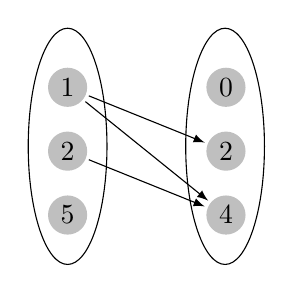
\begin{tikzpicture}
[mydot/.style={circle, fill=lightgray, inner sep=5pt}, >=latex, shorten >= 1pt, shorten <= 1pt]

% Left set:
\node[mydot,                    label={center:1}] (a1) {}; % 1
\node[mydot, below=0.3cm of a1, label={center:2}] (a2) {}; % 2
\node[mydot, below=0.3cm of a2, label={center:5}] (a3) {}; % 5
	
% Right set:	
\node[mydot, right=1.5cm of a1, label={center:0}] (b1) {}; % 0
\node[mydot, below=0.3cm of b1, label={center:2}] (b2) {}; % 2
\node[mydot, below=0.3cm of b2, label={center:4}] (b3) {}; % 4

% Arrows for the relations:
\path[->] (a1) edge (b2);                                  % 1 -> 2
\path[->] (a1) edge (b3);                                  % 1 -> 4
\path[->] (a2) edge (b3);                                  % 2 -> 4

% Ellipses around the sets:
\draw (0.0,-0.75) ellipse (0.5cm and 1.5cm);
\draw (2.0,-0.75) ellipse (0.5cm and 1.5cm);

\end{tikzpicture}
\end{figure}
% https://tikz.dev/tikz-transformations
% see:
% https://tex.stackexchange.com/questions/157450/producing-a-diagram-showing-relations-between-sets
% https://latex.org/forum/viewtopic.php?t=21987
% It's actually the "<"  relation - maybe mention it in the section about orders...but that doesn't really fit well because in orders domain and codomain are the same
There are a couple of important features that such a relation may or may not have. In a \emph{left-total} relation, every element in the left set has an outgoing arrow emanating from it. In a \emph{right-total} relation, every element in the right set has an incoming arrow. In a \emph{right-unique} relation, every element in the left set has at most one outgoing arrow. The naming convention reflects the idea that when you pick one element from the left set, the related  element of the right set, if any, is uniquely determined. We always know, where we have to go. Likewise, in a \emph{left-unique} relation, every element of the right set has at most one incoming arrow. For every element from the right set, the related element from the left set, if any, is uniquely determined. We always know, where we came from. As we can see, our example relation $R$ actually has none of these features.

\medskip
Notationally, we may write $(a,b) \in R$ when we want to express the fact that $a$ is related to $b$ by the relation $R$. Some authors write this in the shorthand infix notation $a R b$ but that looks kinda ugly. For most relations, we'll use special symbols such as $<, \leq, =, \ldots$ such that the infix notation will look nice. 

\medskip
Our example relation above was an example for a general case where we have a relation between elements of a set $A$ and elements of a set $B$. We say that $R$ is a \emph{relation between} the sets $A$ and $B$. An important special case of that is when $B$ is actually the same set as $A$. We the say that we have a \emph{relation on} the set $A$. For a relation on a set $A$, there are a couple of more important named features that the relation may or may not have. In the following table, we use the generic infix symbol $\sim$ for our relation and $\nsim$ to indicate that the elements are not in the relation. 

\medskip
\begin{tabular}{c l}
  $a \sim a$                                       & Reflexive     \\
  $a \nsim a$                                      & Irreflexive   \\
  $a \sim b \Rightarrow b \sim a$                  & Symmetric     \\
  $a \sim b \Rightarrow b \nsim a$                 & Asymmetric    \\
  $a \sim b \wedge b \sim a \Rightarrow a = b $    & Antisymmetric \\
  $a \sim b \wedge b \sim c \Rightarrow a \sim c$  & Transitive    
\end{tabular}
\medskip
...TBC...VERIFY
% asymmetry implies irreflexivity

% https://de.wikipedia.org/wiki/Asymmetrische_Relation
% https://de.wikipedia.org/wiki/Antisymmetrische_Relation
% https://de.wikipedia.org/wiki/Transitive_Relation
% https://de.wikipedia.org/wiki/Reflexive_Relation

% explain left/right totality, left/right uniqueness - see Bill Shillito's course on youtube
% use as example A = {1,2,3,4}, B = {0,2,4} and the < relation. R = {(1,2),(1,4),(2,4),(3,4)}
% not left-total due to (4,X) missing
% not right-total due to (X,0) missing
% not left-unique due to (1,4),(2,4),(3,4)
% not right-unique due to (1,2),(1,4)
% explain inverse relations
% reflexive/irreflexive, symmetric/asymmetric/antisymmetric
%   https://www.youtube.com/watch?v=GvNGf9Gki7o 
% transitive
%   https://www.youtube.com/watch?v=O19RpfoxQpA
%   make table like at the end of this video - but verify the definitions - the asymmetry definition
%%  looks fishy. Maybe antimsymmtery is also "wrongly" defined there?
% draw diagrams

% https://byjus.com/maths/relations-and-its-types/
% https://www.toppr.com/guides/maths/relations-and-functions/types-of-relations/

% https://www.youtube.com/watch?v=Tk5_B7w5fiY&list=PLZzHxk_TPOStgPtqRZ6KzmkUQBQ8TSWVX&index=9

% Was sind angeordnete Körper? (Ordnungstheorie)
% https://www.youtube.com/watch?v=RyhUIoif_B8


\paragraph{Functions} are a special kind of relations, namely those relations which are left-total and right-unique. You can think of functions as a definition of a map from a set $A$ to another set $B$. Each element of $A$ gets mapped to some unique element of $B$. You can throw any $a \in A$ at a function $f$ and it will unambiguously tell you, which $b \in B$ your given $a$ is mapped to. If a function is additionally left-unique, we can actually traverse the arrow back to figure out unambiguously, where we came from. We can undo the application of the functional mapping for those $b \in B$ which have an incoming arrow. Such left-unique functions are also called \emph{injective}. If, on the other hand, the function is right-total, i.e. every element of $B$ has an incoming arrow, we call the function \emph{surjective}. A function that is both injective and surjective is called \emph{bijective}. Such bijective functions can be inverted, i.e. undone, for any $b \in B$ and are therefore also called \emph{invertible}.

% explain domain, range, image, pre-image (of elements and whole sets)
% give the condctiosn for functions in math notation

\paragraph{Equivalences} are another special kind of relations. In equivalence relations, the left and right set are actually the same set and a couple of additional properties must be satisfied. The relation must be \emph{reflexive} meaning that every element $a$ must be in relation with itself. They must also be \emph{symmetric} meaning that if the tuple $(a,b)$ is in the relation, then the tuple $(b,a)$ must also be in it. Finally, they must be \emph{transitive} meaning that if the tuples $(a,b)$ and $(b,c)$ are in the relation, then the tuple $(a,c)$ must also be in it. Reflexivity just means that every object is equivalent to itself. The symmetry condition captures the idea that if $a$ is equivalent to $b$ then $b$ is also equivalent to $a$. Transitivity captures the idea that if $a$ is equivalent to $b$ and $b$ is equivalent to $c$, then $a$ is also equivalent to $c$. The prototype of an equivalence relation is the usual equality denoted by $=$ but the concept of an equivalence is more general. It is meant to capture the idea that two objects are interchangeable within a given context. They do not necessarily have to be the exact same object but certainly can be - this is ensured by the reflexivity. For some equivalence relations, we may actually use the $=$ symbol even though another relation may be meant. Sometimes alternatives like $\sim, \equiv, \simeq, \cong,$ etc. are used. The notation for various equivalence relations may vary form field to field and from author to author. 

% ToDo: Move the explanations of transitive, reflexive, etc. under the tabular

% https://www.youtube.com/watch?v=Ogm711KWwaw
% at around 14:00 The identity is the smallest equivalence relation and AxA (the "all-relation"? "universal relation" is the largest)
% https://www.ask-math.com/universal-relation.html

% https://en.wikipedia.org/wiki/Equivalence_relation
% https://mathworld.wolfram.com/EquivalenceRelation.html

\paragraph{Orders} are yet another special kind of relations. They are also a type of relation defined on one set, i.e. the left and right sets are the same. If a set $A$ is equipped with such an \emph{order} relation, the set is said to be \emph{ordered}. An order relation is typically denoted by the symbol $<$ which we read as "less than", i.e. $a < b$ reads as: "$a$ is less than $b$".

...TBC...
% -trichotomy
% -transitivity
% -it can be inverted into >
% -we have also "less than or equal to", "greater than or equal to"
% -partial and total orders 
% -well ordering - well ordered sets have a least element
% -compatibility with operations: if $a < b$ then $a + c < b + c$ for any $c \in A$

% https://en.wikipedia.org/wiki/Order_theory
% https://en.wikipedia.org/wiki/Total_order
% https://en.wikipedia.org/wiki/Partially_ordered_set#Partial_order
% https://en.wikipedia.org/wiki/Ordered_field
% https://de.wikipedia.org/wiki/Ordnungsrelation

% https://math.libretexts.org/Bookshelves/Applied_Mathematics/Seven_Sketches_in_Compositionality%3A_An_Invitation_to_Applied_Category_Theory_(Fong_and_Spivak)/01%3A_Generative_Effects_-_Orders_and_Adjunctions/1.01%3A_What_is_Order

\medskip
As we see, relations are quite flexible and can be used to model several important concepts in mathematics by imposing some additional requirements on the broad and general concept of a relation.
% ToDo: mention some other kind special kinds/classes of relation

%---------------------------------------------------------------------------------------------------
\subsubsection{Set Operations and Relationships}

\paragraph{Set Algebra} Just like we could combine logical propositions via the connectives $\wedge, \vee, \neg, \ldots$ to yield new propositions, there are operations that we can perform on sets to yield new sets. The \emph{intersection} of two sets $A, B$ is denoted as $A \cap B$ and defined to be the set with the elements that are present in $A$ and in $B$, i.e. the set of elements that $A$ and $B$ have in common. If the intersection between $A$ and $B$ is empty, i.e. the two sets have nothing in common, formally denoted as $A \cap B = \emptyset$, we say that $A$ and $B$ are \emph{disjoint}. The visual resemblence of $\cap$ and $\wedge$ is, of course, no coincidence. The \emph{union} of two sets $A,B$ is the set of all elements that are in $A$ or in $B$ where the "or" is again to be understood as an inclusive or. Imagine throwing all contents of sets $A$ and $B$ together into a bucket. You may get doublings for the common elements (i.e. the intersection) but that doesn't matter anyway because set membership does not care about potential multiplicities - but if you want, you can imagine to remove the doublings after throwing the sets together. The notation for the union of $A$ and $B$ is: $A \cup B$. The symbol looks a bit like a cup and resembles the "or" symbol $\vee$ from logic - again no coincidence. There is also a notion of a set \emph{difference} $A \setminus B$ which is the set $A$ minus those elements of $A$ which are also in $B$. You may read this as "$A$ without $B$". [VERIFY!] If we assume that we have some sort of universal set, i.e. the set of all things that we could possibly consider in the current context, we may also define the \emph{complement} of a set $A$, denoted as $\overline{A}$, which is the set of "everything" except the elements of $A$. Here, "everything" refers to our universal set which may depend on the context. If we call this universal set $U$, we could define $\overline{A} = U \setminus A$. Finally, the so called \emph{cartesian product} or \emph{set product} or just \emph{product} of two sets $A$ and $B$, denoted as $A \times B$, is the set of all possible pairs $(a,b)$ where $a$ is an element of $A$ and $b$ is an element of $B$. Here is a summary of these basic set operations:
\begin{eqnarray}
 \overline{A}  =& \{x: \; x \notin A \}                    \qquad &\text{complement} \\	
 A \cap B      =& \{x: \; x \in A \wedge x \in    B \}     \qquad &\text{intersection} \\
 A \cup B      =& \{x: \; x \in A \vee   x \in    B \}     \qquad &\text{union} \\
 A \setminus B =& \{x: \; x \in A \wedge x \notin B \}     \qquad &\text{difference} \\
 A \times B    =& \{(x,y): \; x \in A \wedge y \in    B \} \qquad &\text{product}
\end{eqnarray}
We may iterate the product operation in the following way: Form the product $A \times B$ and then take the result of that and form the product with a third set $C$ to get: $(A \times B) \times C$. What we formally get would be a set of pairs where the first element is itself a pair of elements from $A$ and $B$ and the second element is an element from $C$. Elements of $(A \times B) \times C$ would look like $((a,b),c)$ where $a \in A, b \in B, c \in C$. On the other hand, elements of $A \times (B \times C)$ would be of the form $(a, (b,c))$. Formally, this is a different set, so our set product is formally not associative. However, the set $(A \times B) \times C$ is isomorphic (i.e. of the "same form") to $A \times (B \times C)$ and in many practical applications, what we actually want to form is not a set of nested pairs but rather a set of triples $(a,b,c)$ with no further inner structuring. We will adopt the convention that when we write a set product with multiple factors without any parentheses like: $A \times B \times C$, we mean the set of triples $(a,b,c)$ where $a \in A, b \in B, c \in C$. And this, of course, generalizes to quadruples, quintuples, etc. We will also use the notation $A^n$ to mean a set of $n$-tuples in which each element is from $A$.

\medskip
In addition to these basic and most common set operations, there are a couple of more, less common ones. Some of them are:
\begin{eqnarray}
 A \triangle B =& (A \setminus B) \cup (B \setminus A)      \qquad &\text{symmetric difference} \\
 A \sqcup B    =& A \times \{ 0 \}  \cup  A \times \{ 1 \}  \qquad &\text{disjoint union} \\
 A ^ B         =& \{ f: \; B \rightarrow A  \}              \qquad &\text{functions from $B$ to $A$} 
\end{eqnarray}
The symmetric difference is what remains, if we first form the union of $A$ and $B$ and then subtract the intersection of $A$ and $B$ from that. That is, we also have: $A \triangle B = (A \cup B) \setminus (A \cap B)$. Other possible notations for the symmetric difference are $A \ominus B$ and $A \oplus B$. The disjoint union is an operation in which we throw together the contents of two sets $A,B$ while keeping the elements that came from set $A$ distinguishable from those that came from $B$ by not using the elements of $A$ and $B$ as is but rather using tuples of the form $(a,0)$ and $(b,1)$ where $a \in A, b \in B$. The appended second components serve as tags to indicate from which set the element originally came. The purpose of the disjoint union is that many desirable set theoretic constructions involving a set union work out as desired only for disjoint sets. That's why we first make the sets $A,B$ artificially disjoint via this tuple formation and then take the union of the so created sets of tuples. The set of all possible functions from a set $B$ to a set $A$ is denoted by the exponential notation $A^B$. The notation $\{ f: \; B \rightarrow A \}$ is informal and intended to mean that $f$ is a function with domain $B$ and codomain $A$ [TODO: figure out, if there's a formal notation for this]. The exponential notation is used for a good reason: for finite sets $A$ and $B$, the number of possible different functions from $B$ to $A$ is indeed given by $|A|^{|B|}$.

[TODO: $A^B$, $2^A = \{0,1\}^A = \mathcal{P}(A) $, quotient set i.e. set of equivalence classes]


\medskip
There are a lot of algebraic equations involving these operators.... [TODO: give a rather comprehensive list of useful set-algebraic equations]



% ToDo: mention that the complement is sometimes also written as A^C ...with some different font for the C, mention that the complement must always be taken with respect to some universal set which may depend on the context

% The set difference is also called "relative complement"
% https://en.wikipedia.org/wiki/Complement_(set_theory)#Relative_complement

% https://en.wikipedia.org/wiki/Disjoint_union
% https://en.wikipedia.org/wiki/Symmetric_difference

% https://math.stackexchange.com/questions/1631396/what-is-the-difference-between-disjoint-union-and-union

% Weitz uses a union symbol with a dot above to denote a union of disjoint sets. see:
% https://www.youtube.com/watch?v=RcDjuXLK-Jg&list=PLb0zKSynM2PDUcEEkjv48Y_4N9CBFyzsz&index=7
% at 9:00.  ...don't confuse this with the "disjoint union" operation which artificially makes sets disjoint before froming the union. Maybe explain both notations in the section of set theory 







\paragraph{Subsets} The set algebra can be seen as providing some operations that we can perform on sets. Sometimes, we also want to express certain relationships between sets. Of particular interest is, when one set $B$ contains all the elements that another set $A$ contains (and possibly more). In such a case, we call $A$ a \emph{subset} of $B$ and we call $B$ a \emph{superset} of $A$. The set $B$ may or may not contain other elements, i.e. elements that are not in $A$. If the superset $B$ does indeed contain additional elements, then we call $A$ a \emph{strict subset} of $B$ and we call $B$ a \emph{strict superset} of $A$. These relations are expressed with the notation $\subseteq, \subset, \supset, \supseteq$ as follows:
\begin{eqnarray}
A \subseteq B \;\;  \Leftrightarrow \;\;   x \in A \Rightarrow x \in B&           \qquad & \text{$A$ is subset of $B$} \\
A \supseteq B \;\;  \Leftrightarrow \;\;   x \in B \Rightarrow x \in A&           \qquad & \text{$A$ is superset of $B$} \\
A \subset   B \;\;  \Leftrightarrow \;\;   x \in A \Rightarrow x \in B,& A \neq B \qquad & \text{$A$ is strict subset of $B$} \\
A \supset   B \;\;  \Leftrightarrow \;\;   x \in B \Rightarrow x \in A,& A \neq B \qquad & \text{$A$ is strict superset of $B$}
\end{eqnarray}
% Alignment is ugly! Maybe use a tabular environment
With the subset relation defined, we can also define yet another operation on sets: taking the set of all subsets of a given set $A$. This operation is called taking the \emph{power set} and the power set of a set $A$ is denoted by $\mathcal{P}(A)$ or by $2^A$ where the latter notation is motivated by the observation that, if the set $A$ has $n$ elements, then the power set will have $2^n$ elements. This also explains the name "power set". Formally, the power set can be written as:
\begin{equation}
  \mathcal{P}(A) = 2^A = \{x : \; x \subseteq A \}
\end{equation}
Here, the elements $x$ of the power set $2^A$ are themselves sets - namely, subsets of $A$. The empty set does also count as a subset of any nonempty set. If a set has $n$ elements, then the number of subsets with $k$ elements is given by the binomial coefficient "$n$-choose-$k$". [VERIFY, REF needed]. The fact that the power set of a finite set $A$ with $n$ elements has $2^n$ elements can also be understood as follows: For each subset, we may define a function $f$ from $A$ to the set $\{0,1\}$ which maps an element $a$ of $A$ to $1$, if the element $a$ is to be included into the subset and to $0$ if the element $a$ is not to be included. For such a function $f$, there are $2^n$ different possibilities because for each element $a \in A$ (of which there are $n$), we can choose either $0$ or $1$ as the mapped value. Including an element into a subset or not is a binary decision. We can establish a bijection between the subsets of $A$ and the set of possible functions $f: A \rightarrow \{0,1\}$, so these sets must have the same number of elements - namely, both have $2^n$ elements.

\paragraph{Cardinality} While we are speaking of the number of elements of a set, i.e. the "size" of a set, it should be noted that this size has been given a special name: \emph{cardinality}. We do not simply call it "size" because there are different notions of set size in mathematics and cardinality is just one of them (another one would be the so called \emph{measure}, for example). In the case of finite sets, the cardinality is just the number of elements, i.e. a natural number (to be defined in the next chapter). For infinite sets, however, set sizes are given by the so called \emph{cardinal numbers} the investigation of which is a whole branch of math on its own. The natural numbers are the finite cardinal numbers - but there are infinite cardinal numbers, too. And yes, that means there are different sizes of infinity in math. In a sense that can be made rigorous, there are more real numbers than natural numbers, for example. The cardinal number of the set of real numbers is bigger than that of the set of natural numbers. The notion of cardinality for infinite sets is defined in terms of existence of bijections: If for two infinite sets, you can find a bijective function between those sets, then these sets have, by definition, the same cardinality. This has a couple of counterintuitive consequences, one of which is that a strict subset of an infinite set can have the same cardinality as the whole set. The part is \emph{not} smaller than the whole. For example, the set of natural numbers and the set of even numbers have the same cardinality. The required bijection and its inverse are simply the functions $y = f(x) = 2 x$ and $x = f^{-1}(y) = y / 2$. But this stuff is beyond the scope of this book. [TODO: give equations for cardinalities]

\paragraph{Relations vs Operations}
We defined a function to be a special kind of relation (left-total, right-unique) and we also intuitively characterized a function as a sort of operation with an input and an output. The operational viewpoint is the way, we usually think of functions: we put some object in and get some object out. It is important to realize that such an "operational" point of view is not necessary. From a set-theoretic point of view, the "relational" point of view is all there is: a function is just a special kind of relation and a relation is just a special kind of set consisting of ordered pairs and ordered pairs can also be thought of a special kinds of sets. The definition really says nothing at all about a function being an input/output "operation". This is merely our interpretation. Or maybe it's more appropriate to say, that an input/output device is something that we want to \emph{model} with the concept of a function. At the core, it all just boils down to specific sorts of sets, because in set theory, sets are really the only thing that we have to work with anyway.

\medskip

A similar consideration can be applied to equivalences. By definition, they are also just a special kind of relation. When we use equivalences, for example to simplify equations, we sometimes interpret an equivalence as a possible replacement rule that can be applied to (parts of) a formula, i.e. a sort of operation. That's not what an equivalence is, at its core, though. It's a common misconception to think of the equals sign $=$ as a prescription to do something like an assignment or replacement when in reality, it just expresses the fact that two things are equal. An equation like $E = m c^2$ can indeed be used to compute $E$ when $m$ and $c$ are known but $E$ is yet unknown and that's indeed how we often use equations: to compute an unknown value from known ones. But the equation in and of itself, at its core and by its nature, is not an algorithmic prescription for a computation. It's just a relation.

%there's not really an intrinsic input/output interpretation
%-explain the relational and operational aspects of 
% -functions (is-related vs input-output) 
% -equivalences (is-equivalent-comparisons vs assigments in programming and simplifications in math)
% -subset relations (is-a-subset vs form/extract-a-subset)
% -explain bi- and multivariate functions (using a set-product as input), 
% -functions of a scalar that yield vector outputs (parametric curves) using a set-product as output
% -explain multifunctions such as the n-th root of a complex number
% -explain the notation f: A -> B
% -explain how the interpretations of two-input/one-output functions: A x B -> C and one-input/two-output function A -> B x C can be though of as ternary relations, i.e. subsets of A x B x C where formally A -> B x C is *interpreted* as A x (B x C) and A x B -> C as (A x B) x C but the interpretation can be "flattened out" and we can do partial application, currying, etc.



% what about relational algebra? useful for databases, I think

% https://texample.net/tikz/examples/set-operations-illustrated-with-venn-diagrams/
%Cardinality

% Union set: A bing cup/union symbol U X means the union of all elements of X. We assume here that each element of X is itself a set - which in set theory is true because there are no other things than sets anyway

% https://www.youtube.com/watch?v=szfsGJ_PGQ0
% The Axiom of Choice

% https://www.youtube.com/watch?v=szfsGJ_PGQ0
% 26:00 - well ordering theorem - explain connection to statement that complex numbers can't be ordered - this seems to be a contradiction - but "being ordered" for complex numbers requires more - the order must be compatible with the arithemtic operations - this is a difference of meaning which is confusing and should be pointed out.



\subsection{Category Theory}
Category theory is an area of math that attempts to structure and organize mathematics itself. This section here is meant to only give a very superficial birds eye overview. Category theory has been called the "mathematics of mathematics" and - less charitably - as "abstract nonsense". Its relation to set theory has been compared to that of higher level programming languages to machine code. Category theory describes a given field of mathematics in terms of a so called \emph{category}. Such a category consists of a class of \emph{objects} and relationships between those objects, called \emph{morphisms}. You can picture the objects as nodes (as in a multigraph, see [REF needed to Graph Theory section]) and the morphisms as directed edges, depicted as arrows. Morphisms are also sometimes called arrows. The category must also have a notion of composing morphisms. When there's an arrow from node $A$ to node $B$ and another arrow from node $B$ to node $C$ then this induces an arrow from node $A$ to node $C$. This sort of \emph{composition} of morphisms into other morphisms can be pictured as traversing a path in the multigraph. The composition of morphisms must be associative. As final ingredient for a category, we need for each node a special kind of morphism, called an \emph{identity}. An identity is a morphism/arrow that goes from a node $A$ to itself and is meant to convey an abstraction of the idea of an identity function - a sort of neutral element in the realm of morphisms.
%ToDo: composition (-> paths), identites (-> loopy edges)

% https://en.wikipedia.org/wiki/Multigraph

\paragraph{The category "Set"} is perhaps the most immediate and prototypical example of a category. In Set, the objects are sets and the morphisms are functions. Composition of morphisms is the usual compositon of functions and the identites are of course the respective identity functions for each set. Don't make the mistake of thinking about set elements as objects. The sets themselves are the objects and their internal structure is considered opaque. From a categorical point of view, we can't look into the sets. We can't talk about individual elements at all in categorical terms - the reason being that, in general, the objects can be of a completely different nature and don't need to have a concept of "elements". One object in Set would be $\mathbb{N}$, another one would be $\mathbb{R}$, another one would be $\{0,1\}$, etc. The category Set has a node for every possible set and for every possible ordered pair $(A,B)$ of nodes (i.e. sets), it has bunch of directed edges (arrows) where each such arrow stands for a possible function from set $A$ to set $B$. For example, there would be an arrow called "$\sqrt{\; \;}$" from $\mathbb{N}$ to $\mathbb{R}$. There would also be a "$\sqrt{\; \;}$" from $\mathbb{R}$ to $\mathbb{R}$ and one from $\mathbb{N}$ to $\mathbb{N}$. As morphisms, they would all be considered different entities even though they are supposed to stand for the same mathematical operation of taking the square root. Each morphism carries along with it its source (or domain) and target (or codomain). Functions can have certain properties and the most important ones are injectivity, surjectivity and bijectivity. Within the framework of set theory, these properties are defined in a way that references set elements. For example, a function from $A$ to $B$ is defined to be bijective, iff every element $a \in A$ maps to a unique element $b \in B$ and vice versa.

% Other examples:
% category of proofs: objects: propositions, arrows: deductions

\paragraph{Iso-, Mono- and Epimorphisms}
Abstracting the idea of bijective functions to a more general setting in which the objects are not necessarily sets and the morphisms are not necessarily functions leads to the categorical idea of an \emph{isomorphism} which is a particular kind of morphism with certain additional properties. The key here is that in the definition of what properties such an isomorphism must satisfy, we are not allowed to talk about "elements". The only things that we are allowed to talk about are categorical terms like objects, morphisms, compositions and identities. We must capture the idea of bijectivity in terms of these and only these ideas. It goes like this: A morphism $f: A \rightarrow B$ is an isomorphism, if there exists a morphism $g: B \rightarrow A$ such that $g \circ f = id_A$ and  $f \circ g = id_B$. In this context, $g$ is the inverse morphism of $f$ and itself an isomorphism as well. In terms of elements when we are in Set: we take an element $a \in A$, apply $f$ to map it to an element $b \in B$, then apply $g$ to map $b$ back to an element $a' \in A$, then $a' = a$, i.e. we're back to where we started so the whole roundtrip from set $A$ to set $B$ and back to $A$ reduces to an identity operation in $A$. Stated without mentioning elements and therefore generalizable: Applying $f$ first, then $g$ yields a composed morphism that equals the identity in $A$ and applying $g$ first, then $f$ yields the identity in $B$. Note how at no point are we talking about the internal structure of the objects like we did when referencing set elements in the definition of bijective functions. The categorical definition of an isomorphism is not even focusing on the objects at all but it's all about the morphisms. The objects are just the backdrop and our main attention goes to the morphisms. We are indeed looking at things from a higher level than in set theoretical descriptions where we looked \emph{inside} the details of the objects. This is typical of category theoretical definitions and theorems. Likewise, a monomorphism $f: A \rightarrow B$ is characterized by the property that for all morphisms $g,h: C \rightarrow A$, we have that $f \circ g = f \circ h$ implies $g = h$. Monomorphisms generalize the idea of an injective (i.e. left-unique) function. An epimorphism $f: A \rightarrow B$ is defined by the property that for all morphisms $g,h: B \rightarrow C$, we have that $g \circ f = h \circ f$ implies $g = h$. Epimorphisms generalize the idea of a surjective (i.e. right-total) function. [VERIFY] If you don't immediately see why these definitions indeed capture and generalize the ideas of injectivity and surjectivity (I certainly didn't), try reversing the implications. For injectivity/monomorphisms, rewrite $(f \circ g = f \circ h) \Rightarrow (g = h)$ as the equivalent statement $(g \neq h) \Rightarrow (f \circ g \neq f \circ h)$ and draw some picture where $g \neq h$. Then do something similar for surjectivity/epimorphisms. Then pat yourself on the back for having grasped a rather abstract and obscure categorical definition. [TODO: maybe add a figure that shows this].
%pg 482 in Ehrig et al

% https://www.youtube.com/watch?v=H0Ek86IH-3Y
% Initial objects have arrow to all objects, terminal object arrows from all objects

% endomorphism, automorphism, homomorphism - the set of morphisms is also sometimes called "Hom" - why?

%ToDo: 
%-explain the categorical analogs of injective and surjective functions (mono- and epimorphisms)
% -explain why the definitions of mono- and epimorphisms work, i.e. capture the desired idea
% -reverse the implications: g != h  ->  g°f != h°f etc. and draw pictures where g != h and show how that implies the RHS
%-give other examples of categories: FinSet, Grp, Vect, deductive systems, Graph
%-explain subcategories in this context - many other examples actually are subcategories of Set
%-examplin categorical products and coproducts
%-explain functors, natural transformations

% https://en.wikipedia.org/wiki/Category_theory
% https://plato.stanford.edu/entries/category-theory/#Exam

% https://www.youtube.com/watch?v=SmXB2K_5lcA  Category Theory for Programmers: Chapter 1 - Category

% https://www.youtube.com/watch?v=1TvNeFLGMrE  Abstrakter Unsinn? Was ist Kategorientheorie?

% https://math.jhu.edu/~eriehl/context.pdf

% https://texample.net/tikz/examples/tag/diagrams/
% https://texample.net/tikz/examples/labeled-chain/

% The Mathematician's Weapon | An Introduction to Category Theory, Abstraction and Algebra
%https://www.youtube.com/watch?v=FQYOpD7tv30
% "Category theory is the abstraction of composition"
% has some nice examples of categories
% https://www.youtube.com/watch?v=5Ykrfqrxc8o&list=PLoCKNPo3VR0I2wqT2wemCNIlpjdy_Ry_q&index=2
% https://www.youtube.com/watch?v=DrldYpmwN5s

% Maybe draw a diagram for Set with some example objects (sets) and arrows (functions)
% Q\{0} x Q  ->  Q:  (a,b) -> a/b
% R  ->  {0,1}:  a -> 1, if a rational, 0 otherwise 

\medskip 
Of course, there's much more to say about category theory but this very brief overview shall suffice for a book that attempts to focus on applied math. 
\section{Numbers and Arithmetic} 

Mathematics deals with various kinds of numbers, the most important of which are the natural, integer, rational, real and complex numbers. The sets of these numbers are denoted by  $\mathbb{N,Z,Q,R,C}$ respectively. In the given order, the sets further to the left are actually subsets of all the sets further to the right, so we have $\mathbb{N \subset Z \subset Q \subset R \subset C}$. The set $\mathbb{C}$ does not have to be the end of this progression (there are even larger sets such as quaternions, octonions, etc.), but in a very meaningful and satisfying sense, it can be justified to stop at $\mathbb{C}$.

\subsubsection{Natural Numbers}
Natural numbers are the counting numbers $0,1,2,3,4,5,\ldots$. The set of natural numbers is denoted as $\mathbb{N}$. They are indeed "natural" in the sense that we have an intuitive understanding what a number like $3$ means. It is an act of abstraction though, to recognize that a set of 3 apples and a set of 3 orang-utans have something in common, namely that they both have the "size" of 3. Whether or not zero is considered a natural number is a matter of convention. The historical fact that the "invention" (or discovery? TODO: elaborate in a footnote) of the number zero was a rather late development in western mathematics (it was recognized much earlier in indian mathematics) may suggest that the idea of zero is not so natural after all. However, I adopt the convention here that zero is a natural number because especially in the context of computers and programming, it is more often than not more convenient to have zero available in the set. There is no right or wrong here. This is a typical case of a definition for which there is no universal consensus in the math community. If zero is in the set $\mathbb{N}$ per definition but we nevertheless need to make a statement about all natural numbers except zero, the notation $\mathbb{N}^+$ is often used. Conversely, if some author defines zero to not be in the set $\mathbb{N}$ but wants to make a statement about all natural numbers including zero, the notation $\mathbb{N}_0$ is often used.

\paragraph{Arithmetic Operations}
There are some elementary operations that take two natural numbers as input and produce another natural number as output. Operations that take two operands are called binary operations, those that take only one operand are called unary operations. The basic binary operations between numbers are usually introduced in elementary school as addition, subtraction, multiplication and division denoted by the symbols $+,-,\cdot,/$ respectively, where the operator symbol is surrrounded by the two operands (computer scientists call this "infix notation"). The dot for the multiplication is sometimes omitted. Let's recall the laws that additon and multiplication obey. For any natural numbers $a,b,c$, we have:

\medskip
\begin{tabular}{c l}
  $a + b = b + a$                             & Commutativity of addition \\
  $a \cdot b = b \cdot a$                     & Commutativity of multiplication \\
  $(a + b) + c = a + (b + c)$                 & Associativity of addition \\
  $(a \cdot b) \cdot c = a \cdot (b \cdot c)$ & Associativity of multiplication \\
  $a \cdot (b + c) = a \cdot b + a \cdot c$   & Distributivity of multiplication over addition
\end{tabular}
\medskip

We could write down some laws for subtraction and division, too. However, it turns out to be more economic to think of subtraction and division not as elementary operations in their own right but rather to consider them in terms of addition and multiplication of so called inverse elements. We will later define the meaning of $-a$ and $1/a$ and with those definitions in place, the laws above will be sufficient and we don't need extra laws for subtraction and division. But we first need to talk about...
% what about precedence and parentheses?

\paragraph{Divisibility}
A natural number $p$ is said to be divisible by some other natural number $d$, if there exists a natural number $q$, such that $p = q \cdot d$ and $q = p/d$. In this case, we call $p$ the product, $q$ the quotient and $d$ the divisor and we express the fact that $p$ is divisible by $d$ by the notation $d | p$ which we read as "d divides p". For example, $15$ is divisible by $3$, because there exists a natural number, namely $5$, such that $15 = 5 \cdot 3$.
% ToDo: introduce division with remainder: p = q*d + r, introduce symbols for division /, talk about the gcd and lcm
Every number is divisible by itself and by one.

\paragraph{Prime Numbers}
Some numbers have the special property that they are \emph{only} divisible by themselves and by one but have no other divisors. These numbers are called prime numbers and can in a certain sense be seen as the atomic building blocks from which all natural numbers except 0 and 1 are made up. This is meant in the following sense: for any natural number greater than 1, there always exists one and only one way to construct it as a product of prime numbers. We say that the factorization of a number into its prime factors is uniqely determined. However, that uniquness holds only up to ordering of the factors - the order cannot possibly matter because multiplication is commutative. Consider the number 60: We can write it as a product as follows $60 = 2 \cdot 2 \cdot 3 \cdot 5$. It has four prime factors where the factor 2 appears twice. 2,3 and 5 are indeed prime numbers - they cannot be further divided into smaller factors. Prime numbers such as 5 have only one single factor in their prime factorization and that factor is the number itself. The word "prime" can be used as noun or adjective: we can say that 5 is prime and also 5 is \emph{a} prime. In this context, the number 1 is not considered a prime by definition. This is again a matter of definition just as the question whether or not 0 should be considered to be a natural number. In this case, however, there is a consensus in the math community that 1 should be defined to not be a prime (that consensus, however, is actually not that old). Numbers that are not prime are called composite numbers because they are made up by more than one (prime) factor. The fact that any natural number greater than one can be constructed as a product of prime numbers and that this factorization is uniquely determined (up to order of the factors) is actually an important theorem: the fundamental theorem of arithmetic. It was known already to Euclid and appears in his "Elements".
% factorization, fundamental theorem of arithmetic

\paragraph{Powers}
Multiplication can be viewed as iterated addition: In $15 = 3 \cdot 5$, the right hand side can be interpreted as $5 + 5 + 5$, i.e. we add together $3$ copies of the number $5$. In analogy, we can define a new operation as iterated multiplication. This will be useful. For example, in the prime factorization of 60, the number 2 appeared twice and in general for any number, a prime factor of that number may appear multiple times. We want a convenient notation to express something like $2 \cdot 2 \cdot 2$. The notation for this is $2^3$: we write the factor as usual and the "number of times" in superscript. The factor is called the "base" and the "number of times" is called the exponent or, depending on context, also the "power". This operation is called "exponentiation" or "raising to a power". With this new notation, we can write the prime factorization of 60 as $60 = 2^2 \cdot 3 \cdot 5$.  We read something like $2^5$ as: "two to the power of five" or "two to the fifth power" or shorter "two to the five" or "two to the fifth". If the exponent is 2 or 3, as in $5^2$ or $5^3$, we may also say "five squared" or "five cubed" respectively. That comes from the geometric fact that $5^2$ is the area of a square with side length $5$ and $5^3$ is the volume of cube with side length 5.

\medskip
Consider $2^3 = 2 \cdot 2 \cdot 2 = 8$. We have already said that in this context, 2 is called the base and 3 is called the exponent. What if we consider the act of raising some arbitrary number $b$ (like 2 in this example) to the power of 3 as a unary operation (i.e. an operation with only one input where we assume the exponent to be fixed) that we apply to $b$ and imagine we are given only the result of the operation (8, in this case). Can we undo the operation, i.e. figure out, that the base must have been 2? That ought to be possible because no other natural number than 2 will produce 8 when raised to the power of 3. The idea of undoing an exponentiation leads to the idea of extracting the "n-th root". Here $n = 3$, so we want to extract the 3rd root from 8. We write this as $2 =\sqrt[3]{8}$ and say "two is the third root of eight" or  "two is the cube root of eight".

\medskip
Consider $2^3 = 8$ again but now let's assume that the base 2 is fixed and we consider the unary operation of raising 2 to any arbitrary power $p$. As before, we are given the result of the operation - 8 - and we want to figure out that the power $p$ that 2 was raised to, to produce that number 8. Again, this should be possible because no other exponent than 3 will produce 8 when 2 is raised to the power of it. ...

% mention tetration (briefly), list the laws for powers, maybe introduce roots and logarithms



% euclidean algo, gcd, lcm, coprime
% factorial, binomial coeffs

\paragraph{Number Systems}
todo: decimal, binary, octal, hexadecimal, sexagesimal, etc. - base p


\paragraph{Solving Equations}
In the definition of divisibility, we said something like "if there exists a natural number such that...". Such a definition is rather implicit and doesn't really give us any clue how we would go about figuring out whether or not such a number exists. Moreover, if such a number does indeed exist, we may want to know, what that number is. We need an algorithm to find that unknown number! But let's first consider a simpler but similar question: Does a number, let's call it $x$, exist such that $3 + x = 5$ and if so, what is it? The question is simple enough that we can solve it by the "method of looking closely" (as my high school math teacher used to say). We immediately "see" that the answer is: "yes, it's two!". But what did we actually do in our minds to figure this out? Maybe we imagined a number line and counted the number of steps that we would have to go to the right from 3 to reach 5? Or maybe we just brute forced the solution by trial and error? Can we do something more systematic and more efficient that we can cast into an algorithm that can then also be applied to more complicated problems for which just "looking closely" doesn't really cut it? 

\medskip
The general theme here is that we want to solve an equation for an unknown variable, which is typically called $x$, just as we did above. The goal is to isolate $x$ on one side of the equation such that it stands there alone. On the other side of the equation we want to see only known quantities, such that we can actually compute that side of the equation directly. Because both sides of the equation are equal (because it's an equation), this computation will give us our formerly unknown number $x$. The strategy to reach this goal is to apply certain allowed manipulations to the equation. So, what kinds of manipulations are "allowed" and why?  We can certainly transform both sides of the equation individually according to the algebraic laws (associativity, commutativity, etc.). But to reach our goal of isolating the unknown $x$ on one side, we will also need some operations in which the two sides interact. These operations should not change the fact that the left hand side (LHS) is equal to the right hand side (RHS). This requirement will be satisfied, iff we do the \emph{same thing} to both sides. If we subtract $3$ from both sides of the equation $3 + x = 5$, we will get $3 + x - 3 = 5 - 3$ which simplifies to $x = 2$ and we are done. This was a very simple example. In general, we may have to combine many manipulation steps, one after another and in just the right order to reach our goal. This process can become arbitrarily complicated  and it may require some experience and intuition to figure out, which transformations will bring us closer to our goal in a given situation. It can also turn out to be impossible for a given equation. Two of the most basic transformations are: (1) add or subtract a constant from both sides, (2) multiply or divide both sides by any constant except zero. There are many more operations that may be ok in a given situation, but some of them come with pitfalls and require special care. For example, you may multiply or divide both sides by the unknown $x$, too - as long as $x$ is not zero, but since $x$ is unknown, you may not know whether or not that's the case. You may also take the square of both sides, but then you need to be aware that this may create extra solutions wich solve only the squared equation but not the original one, so you may need to sieve out these extra solutions later, etc. We won't go deeper into this here because we need to address a more basic problem first: Even for these most basic transformations given above, we may already run into problems. We could solve $3 + x = 5$, but what about $5 + x = 3$? Let's try to isolate $x$ by subtracting $5$ from both sides: $5 + x - 5 = 3 - 5$ which simplifies to $x = 3 - 5$. But what is $3-5$? There is no such natural number!

%In general, adding or subtracting any given constant number from both sides is an allowed operation.
% multiply both sides by the same number (but not with zero)
% divide both sides by the saem number (we must assume that both sides are divisible by that number)
% taking reciprocals of both sides 
% sqauring both sides...with some care
% But: what if applying a transformation results in a
%\medskip
% "subtractability"

\subsubsection{Integer Numbers}
Within the natural numbers, the equation $3 + x = 5$ has no solution. We could be satisfied with this answer and just say: ok, that particular equation has no solution. In general, this may be reasonable - not every equation that we can write down in mathematics needs to have a solution. But maybe we can do better in this case. If we want to have any chance to solve an equation that doesn't admit a solution within the natural numbers, then our sought solution must be something else. What could that something else be? Well, we need to be able to work with it just like we work with numbers - we want to be able to add, subtract, multiply etc. and we want to be able to mix these new (so far, hypothetical) objects in our operations with the natural numbers that we already have. Thus, we will apparently need some not-so-natural numbers or number-like objects. The first set of "unnatural" numbers that we will define are the negative numbers. Together with the set of natural numbers, they form the set of integer numbers, denoted as $\mathbb{Z}$ (from the german word "Zahl" which means "number"). In reality, you can not take away 5 apples from 3 apples but many bank accounts allow you to go into debt. If you have 30 coins deposited and withdraw 50 coins, your account will go into debt by 20 coins which you will have to pay back later - you've taken a loan. Mathematically, such loan or debt can be modeled by negative numbers, i.e. numbers that are less than zero. That means, in order to arrive at zero (i.e. nothing), you need to add something (i.e. put something in). That's indeed a rather unnatural behavior.  A negative number is written with a minus sign in front of it: a debt of 20 is written as $-20$ and we say: "minus twenty" or "negative twenty". Every natural number except zero has a negative counterpart. In this context, the old natural numbers from 1 upwards are also called positive numbers. Zero is neither positive nor negative - it's just neutrally zero. 

\medskip
In the context of abstract algebra, the number zero is indeed called the "neutral element" with respect to addition because adding zero to any number gives as result just that very same number. Zero is neutral in the sense that it doesn't change anything. In general, a neutral element (with respect to some binary operation) has the property that if it occurs as one of the operands, the result of the operation will just be the other operand. In this context, a negative number like $-5$ is then called the "inverse element" with respect to the number $5$ and vice versa. Two elements are said to be inverses of one another with respect to some binary operation, if putting them as arguments into the operation, the result will be the neutral element of that operation. So, the fact that $5 + (-5) = 0$ shows that 5 and -5 are inverses of each other with respect to addition because 0 is indeed the neutral element of addition. For both, 5 and -5, we call 5 the "absolute value" of the number and we capture the idea that 5 is positive and -5 is negative by its "sign" which can be either positive (plus) or negative (minus). Instead of 5, we may also write $+5$, but the plus sign is usually omitted.

\medskip
We have \emph{defined} the negative numbers in terms of how we want them to behave with respect to addition. But how should they behave with respect to multiplication? We should we want here? It would be convenient if our old laws for multiplication (associativity, commutativity, distributivity) would continue to hold for our new numbers. If we can make this work, we wouldn't need to unlearn anything and could work with our new numbers in exactly in the same way that we are already used to from our old numbers and we could also mix old and new numbers in expressions without running into any problems. And indeed, it is possible to make this work in one and only one way. We have to define multiplication for the integers in such a way, that the absolute value of the result is equal to the product of the absolute values of the operands and the sign of the result is negative, iff one of the operands is negative and the other is positive. In particular, the product of two negative numbers has to be positive.


\subsubsection{Rational Numbers}
Motivated by the unsolvability of a particular equation within the realm of natural numbers, we have successfully extended the set of numbers that we have to work with. Now, we are able to solve a far greater set of equations! But there are still some other equations that we cannot yet solve. Consider the equation $3 \cdot x = 5$. Trying to isolate $x$ on the LHS calls for dividing both sides by 3. That will give $x = 5/3$, but just like the expression $3-5$ of which we couldn't make any sense in terms of natural numbers, the expression $5/3$ does not represent any integer number. By trying to solve a particular equation, we have discovered yet another kind of number...tbc...

% rules for arithmetic, countability (Cantor's 1st diagonal argument), decimal expansion (fixed and floating point), explain the notion of a field - the rational numbers are the first example of a field


%\paragraph{Arithmetic Operations}
%... In higher mathematics, specifically in abstract algebra, it turns out that a more convenient way to think about arithmetic operations is to only consider addition and multiplication as basic and cast subtraction and division in terms of these two basic operations and so called inverse elements. The inverse element of a rational number $q$ with respect to addition is just its negative version, i.e. $-q$. The inverse element of $q$ with respect to multiplication is the reciprocal of $q$, written as $1/q$ or $q^{-1}$. The set of rational numbers is the first set in which both of these inverses exist for any given $q$, except for $q=0$ which has no multiplicative inverse. 

\subsubsection{Intervals}
So far, we've built up our number system as $\mathbb{N \subset Z \subset Q}$. In order to approach our next set of numbers, we'll need a little preliminary, so we'll take a small break from extending our set of numbers and have a little interlude.  ....
% open and closed



\subsubsection{Real Numbers}
OK, nice - so the set of rational numbers is a field. We can add, subtract, multiply and divide to our hearts content without ever encountering any object that does not belong to the set (with the sole exception of division by zero). Is that finally good enough or could we still want more? The pattern of coming up with unsolvable equations continues: Consider the equation $x^2 = 2$. We can take the square root of both sides to get the solution $x = \sqrt{2}$. If the square root of two is a rational number, then we can indeed solve that equation within the rational numbers - but is it? The answer turns out to be a resounding nope! I could now present a proof for this fact (and a mathematically minded reader would rightfully demand one) but I think that would distract too much from the main line, so I just ask you to take my word for it.

...tbc...

% completeness, Cauchy sequences

% intervals, uncountability (Cantor's 2nd diagonal argument), algebraic numbers (as subset...but wait - they can be complex, too)

\subsubsection{Complex Numbers}
The set of real numbers forms an ordered, Dedekind-complete field. Does "complete" mean, we are now done with building our number system? Unfortunately not yet. There is still one kind of equation left that we can write down with our basic arithmetic operators but which we still cannot yet solve. But this one will really be the last one, so we see the light at the end of the tunnel! The equation, I'm talking about, is $x^2 = -1$. Solving for $x$ formally yields $x = \sqrt{-1}$, but we know that any real number muliplied by itself will produce a nonnegative result, so this weird square root of minus one cannot be a real number. We will now do a similar step as we did when postulating the existence of negative numbers. Those can thought of as resulting from taking a natural number and multiplying it by some, then hypothetical and unnatural new object - namely, by the number $-1$, which we could call the "negative unit" and which up to then, wasn't a thing.

..tbc...

% what about equations that do not only involve algebraic operations? what if an equation involves transcendental functions? will there still be always a complex solution? or could it make sense to define yet more numbers to solve more equations....like, say tanh(x) = 2...will this have complex solutions? maybe that's the reason why analytic functions are always unbounded over the complex plane, such that they can be inverted for any input?

% https://en.wikipedia.org/wiki/Real_number


% remind of the "unnaturalness" of negative numbers - make the point that imaginary numbers are no more unnatural than negative numbers


\paragraph{Solving Equations, revisited}
....


\paragraph{Are we done?}
I promised that $x^2 = -1$ will be the last equation that we can write down using only the numbers we have and our basic arithmetic operations and that the complex numbers will enable us to solve all such algebraic equations. But you may ask what about $0 \cdot x = 1$? Solving for $x$ formally gives $x = 1/0$ and we know that we can't (yet?) divide by zero. Is it conceivable that we again broaden our notion of what a number is and invent another kind of "imaginary unit" for the strange object $1/0$? Perhaps a sort of "infinite unit"? In certain contexts, the set of complex numbers is indeed augmented by an additional element, called the "point at infinity", denoted as $\infty$, and the resulting set is called the extended complex plane. Having $\infty$ available, we can indeed write down things like $1/0 = \infty$ and also $1 / \infty = 0$. But there is a caveat: We also have $2/0 = \infty, -3/0 = \infty, (4 + 5 \i) / 0 = \infty $ etc. Any finite number divided by zero would have to give infinity as well. But why? Can't we make $2 \cdot \infty$ be something different than $\infty$? I don't really know but I think the current state of the art is that from  $1/0 = \infty$ we can't conclude that $1 = 0 \cdot \infty$, so this notion of infinity doesn't really help us to solve equations uniquely so the usefulness of that idea is a bit limited. In most situations, the equation $0 \cdot x = 1$ is usually indeed just accepted to be unsolvable. Maybe someday someone will come up with a concept of a number that makes that equation solvable, too. I tried myself - and failed, so far....

\medskip
The complex numbers are by many people seen as very mysterious, inscrutable and unintuitive objects. By analogy, I tried to make the point that they are actually no more mysterious or more imaginary than the negative numbers, but I'm not sure, whether I buy that argument myself. So, if you still feel uncomfortable about them and consider them mysterious - don't worry: you are not alone. Welcome to the club! Perhaps for this reason, in my high school math education, they were never mentioned - the reals were, where they stopped. I find that sad because it feels a bit like stopping one step before the finishing line. Maybe that has changed and/or is different in other countries, which I certainly hope because from a mathematical point of view, the complex numbers - and not the reals - mark the logical and satisfying endpoint of a progression of discovering ever more numbers.

% also talk about the extended complex plane, i.e. with the additional point at infinity

\subsubsection{Other Numbers}
What? There are still other numbers? Didn't I just say, the complex numbers mark the endpoint? It is indeed true that we do not need to invent other numbers if the goal is to be able to solve algebraic equations (at least, if we exclude the nasty division-by-zero case). But there may be other goals and other applications in which other notions of a "number" may be useful. That raises the question, what a number actually is. We initially used (natural) numbers to count things. Then, negative numbers were included to model the state of having "less than zero" of a quantity, i.e. a debt. The rational numbers were introduced to model splitting a quantity into equally sized chunks. Later we broadened our scope to use real numbers for a continuously measurable quantity such as a length in geometry. 
%-make small paragraphs about: ordinal, cardinal, hyperreal, dual, p-adic, surreal, clifford numbers (aka multivectors), quaternions, octonions, sedenions, algebraic numbers, modular integers, Galois fields - what about matrices as representations? ...what about wheel theory?

\begin{comment}

-introduce sum and product notation

-say something about countably and uncountably infinite sets (defined via power sets) - real numbers are uncountable but it's yet unknown if their cardinality is aleph1 or aleph2, i think
-numbers in the computer: 2-complement integers, IEEE754 float (half/single/double/quad), big int, big float, overflow, precision, precision loss in subtraction of similar values

\end{comment}



\section{Elementary Algebra}
Now that we have numbers, we want to do something with them. One thing we can do is to perform elementary operations such as addition and multiplication on given numbers to generate new numbers. For example $3 \cdot 5 + 7 = 22$. Hey - cool - we have produced a $22$ from $3,5$ and $7$! Not yet impressed? Then consider this: assume that the number $5$ is unknown and we only know the relation $3 \cdot x + 7 = 22$. Can we recover the unknown $x$ from that equation? It turns out that the answer is yes, we can: by subtracting $7$ from both sides of the equation and then dividing both sides by $3$, we recover $x = 5$. Elementary algebra is the science of solving such equations for unknown variables where it is understood that the unknowns are supposed to be numbers. The setting is usually as follows: we have given one or more equations that contain one or more unknown variables, typically denoted by letters from the end of the alphabet such as $x,y,z$. The question is if there are any solutions of the given equations, i.e. any assignments for the variables that make the equations hold true - simultaneously, if there's more than one equation. If there are solutions, we may ask how many there are. Just one solution, i.e. a unique solution? Or some other number of solutions? Or maybe even infinitely many? And, of course, we may also want to know, what the solution is or what they are. How can we produce them in a systematic way? Elementary algebra is about answering questions like these. Surpassing the "elementary" qualifier, the higher levels of algebra investigate mathematical systems which are then called algebraic structures and it turns out that our familiar natural, integer, rational, real and complex numbers are just specific examples of such systems which are studied there in an abstract way. In this realm of \emph{abstract algebra}, our familiar number systems serve as prototypes which are subsequently generalized. But this stuff is for later chapters. 

% Field theory gives a systematic answer to the question of solving polynomial equations

%We need to learn to walk before we can run.

%It is this realm abstract algebra that will

%An equation may or may not have a solution within the number system that we are working in. 

%Sometimes, different sequences of operations will produces the same result. When different computations produce the same result

% Consider 3 * 5 + 7 = 22. Can we reverse the process? Let's assume, the 5 is not given and we only
% know the relation 3 * x + 7 = 22
%
%   4 * 5 + 2 = 22
% 
% We could also have 4*x + 2 = 3*x + 7 given  -> sub 3*x and 2 on both sides -> x=5

%That something is computation ...tbc...

% Complex conjugation is an automorphism on C that fixes R. That means it can be pulled out or 
% shoved in in all the operation: conj(z * w) = conj(z) * conj(w), etc. - it works also for +,-,/

%===================================================================================================
\subsection{Equations}

%===================================================================================================
\subsection{Arithmetic}
Arithmetic is about performing the elementary operations of addition, subtraction, multiplication and division and on a higher level also exponentiation and extraction of roots. I would argue that when taking roots is included, taking logarithms should be included as well for consistency (both operations are ways of inverting the exponentiation), but that's usually not listed among the arithmetic operations. Be that as it may, we will look at logarithms in this section, too. We will also learn sum and product notation, the factorial and binomial coefficients...tbc...

% Maybe mention also, how the operatioons succesion, addition, multiplication, and exponentiation
% build up on each other and how this could continue with tetration etc.
% https://www.youtube.com/watch?v=u1x_FJZX6Vw
%
% Explaing infinte sums, products and continued fractions
%
% In a section about mathematical constants, explain how formulas for the they can be generated in
% a systematic way using continued fractions and the conservative matrix field. this should be a
% an optional section with asterisk

% https://en.wikipedia.org/wiki/Arithmetic

%---------------------------------------------------------------------------------------------------
\subsubsection{Factorials and Binomial Coefficients}


% What Lies Above Pascal's Triangle?
% https://www.youtube.com/watch?v=q2daqMR3l24


%---------------------------------------------------------------------------------------------------
\subsubsection{Notation for Sums and Products}
% Maybe include continued fractions, too

% Endliche Summen und Produkte / gaußsche und geometrische Summenformel
% https://www.youtube.com/watch?v=O_MI8V8MEkU
% Ein paar einfache Regeln für Summen - Indexverschiebung, Aufsplitten, ...

%---------------------------------------------------------------------------------------------------
\subsubsection{Some Important Formulas}

\paragraph{The Binomial Theorem}

\paragraph{Sums of Powers}
Consider the task of summing all natural numbers up to some given upper limit $m$. That means, we want to compute the sum $S = \sum_{n=1}^{m} n$. Doing it the naive way would require us to perform $n-1$ additions. That's a lot of work when $m$ is large. It turns out that there is a simple formula for that: $S = (m (m+1)) / 2$. [VERIFY]
%  Gauss's Sum and Faulhaber's Formula

% https://de.wikipedia.org/wiki/Gau%C3%9Fsche_Summenformel
% https://didaktik.mathematik.hu-berlin.de/user/Euler.pdf  


% Binomial theorem, Faulhaber's formula (small special cases)


% (x+1)(x-1) = x^2 - 1
% (x+y)(x-y) = x^2 - y^2
% generally:
% (x+y)(x-y) = x^2 - xy + yx - y^2 = x^2 - y^2 + [y,x] = x^2 - y^2 - [x,y] where [.,.] is
% the commutator

%===================================================================================================
\subsection{Linear Equations}


%---------------------------------------------------------------------------------------------------
\subsubsection{Simultaneous Linear Equations}






%===================================================================================================
\subsection{Polynomial Equations}

%---------------------------------------------------------------------------------------------------
\subsubsection{The Quadratic Equation}

%---------------------------------------------------------------------------------------------------
\subsubsection{The Cubic Equation}
% special cases - "depressed cubic"

%---------------------------------------------------------------------------------------------------
\subsubsection{The Quartic Equation}

% Shows a managable formula for th 4th degree equation at 0:20:
% https://www.youtube.com/watch?v=OkaEPi_hYdk

%---------------------------------------------------------------------------------------------------
\subsubsection{Equations of Higher Degree}






\begin{comment}

ToDo:

-introduce positional number systems, in particular decimal and maybe binary as alternative
-give algorithms for long addition, subtraction, multiplication, division
-maybe also for numbers in scientific notation, i.e. floating point numbers
-introduce sum and product notation
 -maybe with a spoiler to infinite sums, use $\sum_{k=1}^{\infty} (1/10)^k = 0.1111... = 1/9$ as example
-introduce sums, products, factorials and binomial coefficients
-but maybe that stuff should go into the "Elementary Algebra" section because it involves 
 variables

References:

https://en.wikipedia.org/wiki/Arithmetic
https://www.britannica.com/science/arithmetic
https://en.wikipedia.org/wiki/Positional_notation
https://en.wikipedia.org/wiki/Mixed_radix


\end{comment}


%\subsection{Elementary Algebra}
%Elementary algebra is about solving an equation for an unknown variable, typically denoted as $x$. This is done by isolating $x$ on one side of the equation and moving all known quantities to the other side. On this other side, no unknown quantity should occur anymore such that it can be directly evaluated. ...tbc...
% example 2 x + 3 = 9 -> 2 x = 6 -> x = 3
% Really ...is it? Or is elementary algebra more generally "computation with letters"?
% ...yep...wikipedia says so


\begin{comment}

ToDo:
-make a (sub)section "Algebraic Reasoning" analogous to the "Geometric Reasoning" section in the Geometry chapter, so we can refer from there to here for analogies

References:

https://en.wikipedia.org/wiki/Elementary_algebra
https://en.wikipedia.org/wiki/Equation

Factoring a sum (or difference) of two cubic terms into a linear and quadratic factor: 
  a^3 + b^3 = (a + b) (a^2 - a b + b^2)
  a^3 - b^3 = (a - b) (a^2 + a b + b^2)
Can be put near the binomial formulas

I think, there's some formula to factor x^n - 1  into  (x-1) * ... ...or something similar. 
Not sure. could also be x^n + 1 = ...  Figure out! I think:

  (x^n - 1) = (x - 1) (1 + x + x^2 + x^3 + ... + x^{n-1})

It can be found by considering the equation x^n - 1 = 0 with root r = 1 and then factoring out
the linear factor (x-r) i.e. (x-1) by polynomial division. I think it can be generalized to

  (x^n - a) =  (x - r) (r^n + r^{n-1} x^1 + ... + r^2 x^{n-3} + r^1 x^{n-2} + r^0 x^{n-1})
  
where r = \sqrt[n]{a}...but this needs to be verified! I'm not sure. Example for the special case 
with a = 1, n = 4:

 (x - 1) (x^3 + x^2 + x + 1) = x^4 + x^3 + x^2 + x - x^3 - x^2 - x - 1
                             = x^4 - 1



Maybe this whole section should be called Elementary Algebra.
This video says (at 5:25):
https://www.youtube.com/watch?v=FQYOpD7tv30
(elementary) algebra is the study of abstraction applied to numbers. 

One could perhaps also say: algebra is computing with letters ("Rechnen mit Buchstaben"), 
deriving general formulas with placeholders into which we can plug in actual values (numbers).
It's also about algorithms to compute an unknown quantity from known quantities (think 
polynomial division, Gaussian elimination, partial fraction expansion). In this context, a 
formula can be seen as a very simple algorithm. A formula usually translates to a single 
assignment operation in a computer program. ..well, some formulas are a bit more complicated.
The quadratic formula spits out two values due to the +- sqrt..., so it would translate to
two assignments (or more when we use intermediate vars). But something like Pythagoras' 
theorem just translates to the assignment: c = sqrt(a*a + b*b) when we assume that c is the
unknown. A formula like lhs = rhs can often be directly translated into an assignment 
operation which, in the context of algorithms, can be seen as a simple mini "algorithm" made
from just a single assignment. If a is unknown, we would translate Pythagoras to 
a = sqrt(c*c - b*b), so one formula may potentially translate to multiple different of such
mini-algorithms. More complicated algorithms may contain branches and loops. In math notation
branches can be expressed in the form of piecewise defined right hand sides and loops in the
form of sequences. These sequences may actually be infinite in which case we step into
calculus territory. An example would be the Babylonian algorithm to compute a square-root. 
It's defined via an infinite sequence. In this specific case, the sequence is defined
recursively. In general sequences may also be defined in other ways as well (for example,
explicitly...i.e...by a formula for the elements).


What other types of "Computation" could we have? Maybe I should explain the basic algorithms 
for hand-calculations with pen and paper?


About squaring equations:

https://math.libretexts.org/Courses/Monroe_Community_College/MTH_165_College_Algebra_MTH_175_Precalculus/01%3A_Equations_and_Inequalities/1.04%3A_Radical_Equations

https://math.stackexchange.com/questions/568780/why-cant-you-square-both-sides-of-an-equation

It introdces extraneous solutions. Explain that

\end{comment}



\section{Functions}
Functions are like machines that take some input and produce some output. In the case of mathematical functions, these inputs and outputs are usually numbers. There are more general notions, taking other types of inputs and producing other types of output, for example sets, vectors, matrices, etc. but here, we will mainly look at functions that take one number as input and produce another number as output and those two numbers will typically assumed to be real numbers. The output of a function is supposed to depend only on the input and will be uniquely defined in the sense that if you apply the same input to a function multiple times, you will always get the same output. The role of the function is to "map" the input value to its corresponding output value. That's why functions are also sometimes called maps.

% That notion of a function is different from the notion of a function in imperative programming where the output of functions can depend on all sorts of internal and external state.

% Functions may also be called "maps":
% https://en.wikipedia.org/wiki/Map_(mathematics)

%===================================================================================================
\subsection{Domain and Range}
The two sets (of numbers) from which inputs can be taken and outputs will be produced are called the \emph{domain} and \emph{range} of the function respectively. Functions are usually denoted by lowercase letters such as $f,g,h$ etc. If a function takes real numbers as inputs and also produces real numbers as output, we write this as: $f: \mathbb{R} \rightarrow \mathbb{R}$. The argument of the function is usually denoted by $x$ and and is written in parentheses and the output is often denoted by $y$. When we write something like $y = f(x)$, we mean that the function $f$ produces the number $y$ as output when we give it the number $x$ as input. An example could be $y = f(x) = x^2$. The function would just square the input and return that as result. 

%\medskip
\subsubsection{Codomain and Image}
There is a little ambiguity with respect to the notion of range. It may mean either one these two things: sometimes it may mean the set of numbers from which outputs can \emph{potentially} be drawn and sometimes the (possibly smaller) set of numbers, that can \emph{actually} be the result. For example, if the domain of $f(x) = x^2$, is taken to be the set real numbers $\mathbb{R}$, we could think of $f$ as a mapping between real numbers and real numbers, i.e. $f: \mathbb{R} \rightarrow \mathbb{R}$. However, not all possible real numbers are reached because the result of $x^2$ will never be a negative number. We could also consider $f$ as a function from the real numbers to the \emph{nonnegative} real numbers, i.e. $f: \mathbb{R} \rightarrow \mathbb{R}^+_0$. To distinguish these two notions, sometimes the term "codomain" is used for the set that outputs could potentially be drawn from and "image" is used for the set from which numbers are actually produced by the function for a given input domain. You may also find authors talk about the image of a set under a function $f$ where that set is a subset of the domain of $f$. By this, they mean the set of output values that a function produces for the given set of input values. For example, the image of the interval $[3,5)$ under $f(x) = x^2$ is the interval $[9,25)$. The converse of this is called the \emph{pre-image} which is the set of input values that gives rise to a given set of output values. The pre-image of $[9,25)$ under $f(x) = x^2$ is $[3,5) \cup (-5,-3]$, for example. You may sometimes see expressions where a set $A$ is given as an argument to a function $f$, denoted as $f(A)$ or $f[A]$. What is meant by that is the image of the set $A$ under $f$ which is again a set. For the pre-image of a set $B$, you may see notations like $f^{-1}(B)$ or  $f^{-1}[B]$. The bracket notation is actually preferable because it makes clear that a set is taken as input rather than a single (numeric) argument. However, most authors tend to use the more sloppy parentheses notation for both - single arguments and sets of arguments. This may lead to confusion in certain cases. These cases may seem contrived to the beginner but they actually may occur in practice in more advanced math contexts, so we will adopt the bracket notation here.


% https://www.youtube.com/watch?v=3czgfHULZCs
% 1:56:48: injective = into, surjective = onto ...but that sounds questionable

% https://en.wikipedia.org/wiki/Domain_of_a_function
% https://en.wikipedia.org/wiki/Range_of_a_function

% If a set is given as input to a function to produce the image set A, it is better to use bracket rather than parentheses notation, i.e f[A] rather than f(A) (Weitz explains in one of his videos why - it's in the 2023 course, the videoo about function, I think.). Here:
% https://www.youtube.com/watch?v=1DK_5koM-1o&list=PLb0zKSynM2PCLnXVwfjVcefXa6iZA-an4&index=20
% the relevant part starts at around 7:30, 14:58
% Maybe elaborate this a bit

% The codomain "contains" the set of outputs
% https://www.youtube.com/watch?v=szfsGJ_PGQ0

%===================================================================================================
\subsection{Taxonomy}
There are certain features that a function may or may not have which turn out to be important for classification. A function is said to be \emph{monotonically increasing}, if from $a \geq b$ follows $f(a) \geq f(b)$. It means that the function either goes upward or stays constant but never goes downward. If the stronger condition  $a > b \Rightarrow f(a) > f(b)$ holds true, then $f$ is \emph{strictly monotonically increasing}. Such a function really goes upward everywhere. Not even plateaus are allowed. A \emph{(strictly) monotonically decreasing} function is defined analogously with $\leq, <$ rather than $\geq, >$. If a function is either (strictly) monotonically increasing or decreasing, it is called \emph{(strictly) monotonic}. A function $f$ is said to be \emph{bounded from above} when there is some finite number $U$ such that $f(x) \leq U$ for all $x$. The number $U$ is called an \emph{upper bound} for $f$. Likewise, a function $f$ is called bounded from below, when there's some number $L$ such that $f(x) \geq L$ for all $x$. In this case, $L$ is called a \emph{lower bound} for $f$. A function that is bounded from below and above is called \emph{bounded}. A function for which we have $f(x) = f(-x)$ has \emph{even symmetry} and a function with $f(x) = -f(-x)$ has \emph{odd symmetry}. Every function $f$ can be decomposed into an even part $f_e$ and odd part $f_o$ like so: 
\begin{equation}
\label{Eq:EvenOddFuncDecomp}
f_e(x) = \frac{f(x) + f(-x)}{2}, \;\;
f_o(x) = \frac{f(x) - f(-x)}{2}, \qquad
f(x) = f_e(x) + f_o(x)
\end{equation}
\emph{Injectivity}, \emph{surjectivity} and \emph{bijectivity} are also important features which have already been discussed in the section about set theory. To reiterate, injectivity means that different inputs get mapped to different outputs: $x_1 \neq x_2 \Rightarrow f(x_1) \neq f(x_2)$. This is sometimes also called a \emph{one-to-one} mapping. Surjectivity means that all possible numbers from the codomain are reached: $\forall y \exists x: f(x) = y$. A surjective function is sometimes also called \emph{onto} - it maps the domain onto the full codomain. Bijectivity means injectivity and surjectivity, i.e. the function is one-to-one and onto. Bijective functions are \emph{invertible}. If you know the output $y$, you can uniquely figure out\footnote{In principle, you can. It may not be easy, though.}, which $x$ gave rise to that $y$ under $f$. Functions can also be \emph{periodic}. That means that there exists some number $p$, called the period, such that $f(x) = f(x + k p)$ for all inputs $x$ and all integers $k$. Such a function repeats itself over and over. Functions may have \emph{asymptotes} which are straight lines which the function approaches as the argument goes to plus or minus infinity. Asymptotes can also be vertical lines. In this case, the line is approached as the argument approaches a finite value and at that value itself, the function is usually undefined. When a function $f(x)$ has a vertical asymptote at some input value $x_0$, we call $x_0$ a \emph{pole} of the function. A function is said to be \emph{compactly supported}, if it is nonzero only in some finite interval and zero outside that interval. A function is called \emph{convex} if you can pick any two points $(a,f(a)),(b,f(b))$ on its graph, connect them with a straight line and the function will be below that line everywhere. The function behaves like a chain hanging down, i.e. it is curved downward like a bowl. The opposite of convex is \emph{concave}. Such functions are everywhere above the straight line. They look like an arch. A \emph{continuous} function is one that can be drawn without lifting the pencil or drawing vertical lines. Functions can also be classified according to their degree of \emph{smoothness} and/or according to whether or not they have a finite area under their graph. To define exactly what that means, we will need a few tools from calculus (differentiability, integrability), so we will defer further discussion about these features to later chapters.

% surjective: codomain coincides with image?
% "surjective" could better be called "exhaustive". "injective" could be called "unambiguous" or
% "monogamous"

% Is it true that whenever f is injective then its inverse is survjective and vice versa? But no.
% I think, f being injective does not guarantee the existence of the inverse of f. Maybe f is
% injective whenever the inverse of a suitable restriction of f (or f^-1) is surjective? Figure out!

%===================================================================================================
\subsection{Defining a Function}

\paragraph{Explicit Rules}
One way to define a function is to prescribe a simple \emph{calculation rule} such as $f(x) = x^2 + 3 x - 5$ that applies equally to all possible inputs $x$. Up to until a few hundred years, this was the only way that was acceptable for mathematicians to define a function. Today, we have become a lot more liberal in that regard and allow functions to be defined in more esoteric ways. Some of these ways will involve concepts that are discussed only later in the book. If you don't understand these definitions, you can skip them on a first reading. In a first pass, you need to understand only this and the next way.

\paragraph{Piecewise Definitions}
A slightly more complicated way to define a function would be to have different calculation rules for different subsets of the domain. If these subsets are succesive intervals of the real number line, this way of defining a function is called a \emph{piecewise definition}. They are written down like this:
\begin{equation}
f(x) = 
\begin{cases} 
 0 \quad& x < 0 \\
 -x     & 0   \leq x < 1 \\
 x^2    & x \geq 1
\end{cases}
\end{equation}
This means, the function will output $0$ for $x < 0$ and $-x$ when $x$ is between zero and one (including zero, excluding one) and $x^2$ when $x \geq 1$. The example function is discontinuous at $x=1$. It jumps from $-1$ to $+1$ there. At zero, it has a corner - that is: a discontinuity in its slope. Discontinuities for function values and/or derivatives at the boundaries of the pieces are a common feature in such piecewise defined functions\footnote{Although it is possible to construct piecewise functions that join smoothly at the boundaries. The so called bump-function is an example for that.}.

% Maybe try to put a small plot next to the definition. There's enough space
% Maybe mention that some authors write "for" or "if" in front of the conditions and/or use commas
% so separate them (in addition to line breaks)

\paragraph{Conditional Definitions}
The piecewise definition is a specific kind of a conditional definition where the conditions are of the form "if $x$ is in interval ... then ...". A function can also be defined by more general conditions such as:
\begin{equation}
f(x) = 
\begin{cases} 
 1 \quad& x \in    \mathbb{Q} \\
 0      & x \notin \mathbb{Q}
\end{cases}
\end{equation}
The function given above is called the Dirichlet function or indicator function of the rational numbers. It outputs one for rational inputs and zero for irrational inputs.

\paragraph{Definition by Data}
A function can also be defined by recorded data points of some measurement. To turn these discrete data points into a continuous function, one would also have to prescribe some sort of \emph{interpolation} rule such as "connect the dots by straight lines". The data together with the interpolation rule constitute a bona fide function: we can give it an input $x$ and it will give back an output $y$. 

\paragraph{Algorithmic}
Functions can be defined by the limit of some infinite recursive process or algorithm. An example of that is Bolzano's function. Such functions will often show self-similar, "fractal" behavior: you can zoom in as much as you like and it will always look similar. 
...TBC...ToDo: explain construction rule
% https://de.wikipedia.org/wiki/Bolzanofunktion
% https://demonstrations.wolfram.com/BolzanosFunction/
% Maybe "Algorithmic" is a too general term here. Maybe use "Recursive" or "Geometric". It's basically a recursively applied geometric construction rule. Maybe "Recursively Geometric". Or "as limit"

\paragraph{Infinite Sums}
The infinite process is sometimes defined to be an infinite sum. The individual terms are defined in terms of already known, simpler functions. An example of such a definition is the Weierstrass function defined as:
\begin{equation}
f(x) = \sum_{n=0}^\infty a^n \cos(b^n \pi x), 
\qquad 0 < a < 1, \; b \in \mathbb{N}, odd, b \geq 7
\end{equation}
It has two tweakable parameters $a,b$. It is defined as an infinite sum of exponentially weighted sinusoidal functions. This function has also a self-similar nature and a couple of strange properties that were unheard of in mathematics up to the 19th century such as being continuous everywhere but differentiable nowhere.
% https://en.wikipedia.org/wiki/Weierstrass_function

\paragraph{Power Series}
Often we will encounter infinite sums of weighted powers of $x$. A function definition based on such a sum is called a \emph{power series} definition. Most of our common functions such as $\e^x, \sin(x), \cos(x), \ldots$ can be expressed as such a power series even though they may have originally have been constructed by other ways. Exponential and sinusoidal functions are usually first defined by means of limiting processes or geometric constructions respectively. However, they do also have power series based definitions. For the mentioned example functions, their power series are given by:
\begin{equation}
\e^x    = \sum_{k=0}^\infty   \frac{x^k}{k!}, \quad
\sin(x) = \sum_{n=0}^{\infty} \frac{(-1)^n x^{2n+1}}{(2n+1)!}, \quad
\cos(x) = \sum_{n=0}^{\infty} \frac{(-1)^n x^{2n}  }{(2n)!}
\end{equation}
Don't worry if you don't understand these formulas at this point. They can be justified using the theory of Taylor expansions which is a topic we will pick up later in the calculus chapter. Power series are often used to expand the domain of a function - for example, from the real to the complex numbers. This works out so nicely because all that we need to evaluate a power series is to know, how to add or multiply two objects together and how to scale an object by a factor. When we have objects on which we have these 3 operations defined, we can evaluate, for example, the exponential function of that object via the above power series. The "object" can be a real or complex number - or it can be something else such as a matrix or an operator. We'll see later what these things are. Of course, such a power series does not need to originate from already known functions. It can be made up in any way you like - you just need to prescribe some rule to compute the weights. How you came up with that rule doesn't matter. What matters is the question, whether or not the series actually converges. More on that in the section about series in the calculus chapter.

\paragraph{Analytic Continuation}
Speaking of convergence, consider the following infinite sum:
\begin{equation}
	f(x) = \sum_{n=1}^\infty \frac{1}{n^x}
\end{equation}
This sum converges only for $x > 1$. If we allow complex arguments, the condition is $\Re(x) > 1$. So in the complex plane, this sum above defines a function for those complex numbers whose real part is greater than one. For other values, the function is as of yet undefined. However, as we will see later, complex analysis provides a tool known as \emph{analytic continuation} by means of which we can uniquely expand the domain of the function to the whole complex plane except for the single point $x=1$. The so defined function is known as the Riemann Zeta function and an important object in number theory due to its unexpected connection to prime numbers. The point that I want to make here is that the process of analytic continuation gives us yet another way to define a function. We may start with an expression that may be valid only for a small subset of the real numbers. Our expression defines a function on that subset - but elsewhere it just doesn't make sense. Analytic continuation comes to the rescue to extend the domain of the function. Often, this extension works for the whole complex plane with possible isolated undefined points.

\paragraph{Continued Fractions}
Another infinite process that is sometimes useful to define a function is called a \emph{continued fraction expansion}...TBC...

\paragraph{Inverse Functions}
A function can be defined by its inverse function. In general, you can take any given function $y = g(x)$ and then define another function $f$ by asking: "for a given $y$, what $x$ would I have to plug into my function $g$ to get that $y$?". For example, the logarithm can be defined to be the inverse of the exponential function. For a slightly more interesting example, consider the function $g(x) = x e^x$. Its inverse cannot be expressed in terms of common functions. Yet, it does have an inverse (with some caveats). The inverse function of $x e^x$ is called the "product logarithm" or "Lambert-W" function and has applications in the solution of equations where an unknown $x$ appears as base and as exponent or inside and outside of a logarithm.
% https://en.wikipedia.org/wiki/Lambert_W_function
% https://en.wikipedia.org/wiki/Lambert_W_function#Applications
% y = x e^x  <->  log(y) = log(x) + x
% https://www.desmos.com/calculator/s3gxvjbovr

% $f(y) = g^{-1}(y)$
%ToDo: arcsin, ...
%$ actually, the Lambert-W function is a case of an inverse function - in this case, the inverse of x e^x. maybe for implicit functions use y e^y = x + sin(x)

% W solves the ODE: y' = y / (x*(1+y)), see:
% https://www.youtube.com/watch?v=cMZ_blqKKZU

\paragraph{Implicit Equations}
Defining a function via its inverse is a special case of an implicit function definition. In a more general setting, we could have a bivariate function of the form $g(x,y) = 0$. In the case of the product logarithm function, we would have $x = y e^y$, so $g(x,y) = 0 = y e^y - x$.  This is an equation that can be solved for $x$ on one side of the equation. That's why we can define a function in terms of the inverse of the other side. But that doesn't always have to be the case. Consider modifying the equation $x = y e^y$ to $x + x^5 = y e^y$ or, equivalently $g(x,y) = 0 = y e^y - x - x^5$. Now, we can't  solve for a single $x$ on one side. And, as before, we can't solve for $y$ either. Still, we can ask: "for a given $y$, what value of $x$ can I plug into $g(x,y)$ such that it evaluates to zero?" or "for a given $x$, what $y$ ...". There doesn't have to be a solution and if there is one, it doesn't need to be unique. But if there is a unique solution, then that equation defines a function. If there are multiple solutions, we may pick one of them to be our function of interest. You can play with the function defined by $ y e^y = x + b \sin(a x)$ a bit here on Desmos: \href{https://www.desmos.com/calculator/jfxwuhot8k}{jfxwuhot8k}. Tweak the parameters $a,b$. When any of them is zero, then the function is the regular product-log function. When both are nonzero, we get a wiggly version of it. ...TBC...


% \href{https://www.desmos.com/calculator/t3t92nihws}{t3t92nihws}

% https://en.wikipedia.org/wiki/Implicit_function

% y e^y = x + x^5
% https://www.desmos.com/calculator/ekao9wnrun
% https://www.desmos.com/calculator/t3t92nihws

% y e^y = x + b sin(a x)
% https://www.desmos.com/calculator/izay7xuihf
% https://www.desmos.com/calculator/jfxwuhot8k

% y + sin(y)   = x e^x      a wiggly version of Lambert-W
% y + sin(a y) = x e^x      wiggles get stronger for a > 1, it becomes multi-valued
% https://www.desmos.com/calculator/mowoqggdpj

% x tanh(x) = y atan(y)     has two graphs
% https://www.desmos.com/calculator/9cfsbbm0d9


%Now we want to cosider functions defined by so called \emph{implicit equations}. These are equations of the form $g(x,y) = 0$ for some given function bivariate $g$. They define a set of points in the $xy$-plane. Now, we can define a function $y(x)$ by requiring that it should satisfy our implicit equation, i.e. $g(x,y(x)) = 0$ is satisfied for all $x$ in some domain. That's an implicit definition for $y(x)$. For example, we could require the following equation to hold:
%\begin{equation}
% y e^y = x \;  \Leftrightarrow \; x - y e^y = 0 
%\end{equation}
%In this case $g(x,y) = x - y e^y$. I did not make up this example. The so defined function $y(x)$ is called the "Lambert-W" function or "product-logarithm" function. 

% Move that into the Interlude:


\paragraph{Interlude - Evaluation}
Of course, an implicit definition tells us nothing at all about how we would go about evaluating $y$ for a given $x$. Nonetheless, it is a valid definition of a function. Function definitions do not necessarily need to prescribe an explicit evaluation algorithm. Mathematical definitions in general are not always constructive. They are supposed to tell us \emph{what} it is, not \emph{how} we may compute it. If they do tell us how to compute it, that's a bonus. There are algorithms to solve such implicit equations numerically, though. But that's a topic for a later chapter. You may also wonder how we are supposed to evaluate functions that are defined by some infinite process. The answer is: on a computer, we cannot really represent real numbers exactly anyway. Our usual floating point numbers are always approximations. They attempt to approximate the real numbers - but can do so only up to a finite precision. So, from a practical point of view, it is good enough to be able to evaluate functions up to some given precision. For the infinite processes, that usually means that we can obtain a sufficiently precise approximation of the function by only doing a finite number of steps until we deem the result to be close enough. The best we can expect is to be precise within one ulp ("unit in the last place"). Usually, we'll accept even much higher errors.

% Maybe the difference between a function definition and a prescription of an algorithm to evaluate 
% it can be likened to declarative vs imperative programming? When one says fac(0) = 1, 
% fac(n) = n * fac(n-1) for n > 0, one just declares a mathematical rule without saying how to 
% evaluate they factorial function. The definition may strongly suggest a recursive implementation 
% but it doesn't really prescribe one.



\paragraph{Functional Equations}
Now let's consider the factorial function $n! = 1 \cdot 2 \cdot 3 \cdot \ldots \cdot n$. As it stands, it's defined only for natural numbers. There is a way to define it for all real and even complex numbers. The key lies in the observation of the factorial's functional equation\footnote{A functional equation is an equation that relates values of a function at different evaluation points. Here, it relates the values of the factorial function at the evaluation points $n$ and $n-1$.} which is given by $n! = n \cdot (n-1)!$. In our expanded definition, we want that equation to be satisfied for all real inputs. So we search for a continuous function $f(x)$ for which the functional equation $f(x) = x \cdot f(x-1)$ holds true. It can be shown\footnote{At this point, don't worry about \emph{how} this can be shown and worry even less about how one would come up with these formulas in the first place.} that the following integral based definitions:
\begin{equation}
\Pi(x)    = \int_0^\infty t^x e^{-t} \, dt, \quad
\Gamma(x) = \Pi(x-1) = \int_0^\infty t^{x-1} e^{-t} \, dt,
\end{equation}
do indeed lead to functions that satisfy the desired functional equation. The first definition agrees with the factorials at the naturals, i.e. $\Pi(x) = x!$ for $x \in \mathbb{N}$. That means, it interpolates (i.e. makes continuous) the formerly discrete factorial function. The second definition is called the \emph{gamma function} and it agrees with the shifted factorial function. There is some discussion on \href{https://math.stackexchange.com/questions/1362523/why-is-the-gamma-function-off-by-1-from-the-factorial}{stackexchange} about why the gamma function might have been defined with that strange shift. Supposedly, it will make some higher level math more convenient and I am in no position to verify or falsify that claim. At first, it certainly seems more unnatural and inconvenient than the $\Pi$ function. Nevertheless, it's the gamma function that is used in math all over the place. So, when translating between the discrete factorial and the continuous gamma function, be wary of "off by one" errors. But be that as it may - my point here is that a function definition can be based on a functional equation. 
[VERIFY all of this!]

% Differentiating The FACTORIAL?! | Laid Back Math, Episode 20
% https://www.youtube.com/watch?v=gQKc308e-R4
% has good derivation for why gamma satisfies the functional equation of the factorial

\paragraph{Parameter Integrals}
In this case of the factorial function, the solution of the functional equation led to a definition in terms of a \emph{parameter integral} which is an integral in which the integrand depends on a parameter - here $x$.
I think, the general way to define a function $f$ in terms of a parameter integral is to have some function $g(x,t)$ and then use:
\begin{equation}
 f(x)  = \int_{a(x)}^{b(x)} g(t,x) \, dt
\end{equation}
For $\Pi(x)$ we have $g(x,t) = t^x e^{-x}, a(x) = 0, b(x) = \infty$.
[VERIFY all of this!]
...TBC...
% https://en.wikipedia.org/wiki/Gamma_function
% https://math.stackexchange.com/questions/1362523/why-is-the-gamma-function-off-by-1-from-the-factorial
% https://mathoverflow.net/questions/20960/why-is-the-gamma-function-shifted-from-the-factorial-by-1
% https://de.wikipedia.org/wiki/Parameterintegral
% Arens pg 409 ff, Bärwolff pg 166 (1 example),

\paragraph{Antiderivatives}
Speaking of integrals - we sometimes have a known function $f$ and want to define another function $F$ as an antiderivative of $f$. An important example is the area under a Gaussian bell curve from minus infinity up to some value $x$:
\begin{equation}
 F(x)  = \int_{-\infty}^{x} e^{-t^2}  \, dt
\end{equation}
I think, this can also be seen as another special case of a "parameter integral" definition with $g(x,t)=e^{-t^2}, a(x)= -\infty, b(x)=x$? ...figure out! Explain the erf-function

\paragraph{Differential Equations}
Finding an antiderivative is a problem of the form: for a given $g(x)$, find a function $f(x)$ such that $f'(x) = g(x)$. That equation is actually a special case of a more general class of equations called differential equations. These are equations in which the unknown function $f$ and derivatives of it may appear. A function $f$ that satisfies the differential equation is called a solution of the differential equation. Of course, saying something like: "let $f$ be the solution to the following differential equation..." is also a way of defining a function. There are some caveats, though: differential equations typically have many solutions so we need some additional constraints (typically boundary conditions or initial conditions) to pick out one of those solutions uniquely ...TBC...give examples for how exp and sin can be defined by an ODE, mention Bessel functions
%Having seen how function can be defined via integrals, the next step is consider functions that are defined by differential equations...TBC...

% differential equations - start with simple examples like exp, sin, cos, the give more complex examples like Bessel

\paragraph{Integral Equations}
An integral equation is an equation where an unknown function $f$ appears under an integral sign. Like with differential equations, solving the integral equation amounts to finding $f$. For example, imagine that we have two known functions $g, h$ and we want to find $f$ such that:
\begin{equation}
 \int_a^b f(u) h(x-u) \, du = g(x)
\end{equation}
for some constants $a,b$ (which are often minus and plus infinity). This example is not a contrived one - it has a practical interpretation. We could interpret $g$ as a recorded signal, $h$ as the impulse response or "kernel" of a filter and we want to reconstruct $f$ as it was before it went through the filter. The desired function $f$ appears under a convolution integral. This sort of equation is a particular kind of integral equation and does indeed define a function $f$.

%...TBC...
%ToDo: bring an example involving deconvolution - we are given a signal $g(x)$ which is supposed to be our desired $f(x)$ convolved with some known kernel $h(x)$. Then $f(x)$ appears under the convolution integral. Finding it involves deconvolution...can perhaps be done in the Foruier domain - but that's not the problem of the definition




%\paragraph{Implicit Differential Equations}
% well - so far we have said nothing in the paragraph about diffeqs that restricts us to explicit ones so we may consider the implicit ones to be already subsumed

%What about an implicit differential equation

% Yet another way to define a function:
% https://www.youtube.com/watch?v=U_5JDWR0HiM  Why care about infinite dimensions?
% it uses an (contraction) operator and defines the function as a fixed point of that operator. This coudl aczually be easily implemented numerically, I think.

\paragraph{Fixed Point of an Operator}
This is a fun one and rather exotic and requires some higher level math concepts, so feel free to skip it on a first read. An operator is a higher order function - an object that takes a function as input and returns another function as output. Such operators can have fixed points. These are functions for which the operator returns the input function unchanged - just like the function $f(x) = x^2$ has the fixed point $1$, i.e. returns one when plug in one. With such an operator in hand, we can define the function to be a fixed point of our given operator. [Q: What about eigenfunctions of an operator? Is that a generalization and a fixed point is an eigenfunction with eigenvalue $1$?]

% x^2 has the other fixed point x=0. x=0 is stable and x=1 is unstable, I think.

\paragraph{A Non Function}
Consider the following nonsensical looking attempt of defining a function:
\begin{equation}
f(x) = 
\begin{cases} 
0       \quad& x \neq 0 \\
\infty       & x = 0
\end{cases} \qquad \text{with} \qquad
\int_{-\infty}^{\infty} f(x) \, dx = 1
\end{equation}
We are trying to define a "function" that is zero everywhere except at zero. There, it should have an infinitely tall and infinitely thin spike. The (infinite) height of the spike should be adjusted in such a way that the total area under the function is unity. This "function" is called the Dirac delta function - and it isn't really a function at all because the definition does not really make sense formally because we cannot just treat infinity as if it were a real number. Doing so would lead to contradictions when you try to start computing with it. But when this strange function-like object appears under an integral, it suddenly starts to make a lot of sense and is very useful. We'll meet this bizarre Dirac spike again later in the chapter about functional analysis where it will be more rigorously defined as a \emph{distribution} which is a certain kind of \emph{functional}. Especially in physics and signal processing, we often work with this thing informally as if it were a function.


%ToDo: integral equation
% maybe make these subsubsection of an "Elementary functions"  section

\paragraph{Whoa!} That was a tour de force! I have presented quite a lot of ways how a mathematical function can be defined. Some of them required some rather high level math which doesn't really belong into such an early chapter. I did this to point out that the idea of "defining a function" can, when intepreted liberally as we do in the modern world, include much more diverse and creative ways rather than just a simple and explicit calculation rule. However - most functions that we encounter in everyday life are not of such a complicated nature. There's a set of functions that tends to pop up everywhere and constitutes a sort of basic mathematical vocabulary that everybody needs to be familiar with. I'm talking about the so called...

%===================================================================================================
\subsection{Elementary Functions}
In general, a function can be any mapping. But there is a certain set of functions that permeates mathematics so thoroughly that it has been given a special name: the elementary functions. These are all functions that can be constructed by a finite formula involving only the 4 basic arithmetic operations, roots, exponentials, logarithms, trigonometric functions and the inverses of all these functions.

% https://www.youtube.com/watch?v=l6w868U8C-M
% https://en.wikipedia.org/wiki/Elementary_function

%---------------------------------------------------------------------------------------------------
\subsubsection{Absolute Value aka Norm}
A simple but very important function is the \emph{absolute value} or \emph{norm} of some number $x$ which we commonly write as $|x|$ and read as "absolute value of $x$" or in some contexts also "norm of $x$". The former term applies to real numbers $x$ and the latter term applies in cases where $x$ is a more complicated object than a real number. Yes - that means the absolute value (or norm) function will later be generalized to more complicated objects (complex numbers, vectors, matrices, etc.) and by doing so, it will retain some of its important properties and that's perhaps the chief reason why it is such an important function despite being so humble. For a real number $x$, it can be defined as:
\begin{equation}
 |x| = \sqrt{x \cdot \overline{x}} = 
\begin{cases} 
  x \quad & \text{iff } x \geq 0 \\
 -x \quad & \text{iff } x   <  0 \\
\end{cases} 
\end{equation}
The piecewise definition on the right hand side is how we usually think of $|x|$ when $x$ is a real number. The definition with the square-root in the middle can at this point be taken as a provision for later generalizations and you don't need to worry about this right now, if it doesn't make any sense yet (spoiler: the overline will be used for complex conjugation and the product will generalize to a so called scalar product). Our absolute value function satisfies the following conditions for all $x,y \in \mathbb{R}$:

\medskip
\begin{tabular}{l l}
\label{Tab:Norm}
Non-negative:         & $|x| \geq 0$  \\
Positive definite:    & $|x| = 0 \Leftrightarrow x = 0$  \\
Multiplicative:       & $|x \cdot y| = |x| \cdot |y| $  \\
Triangle inequality:  & $|x + y| \leq |x| + |y| $
\end{tabular}
\medskip
%https://en.wikipedia.org/wiki/Norm_(mathematics)
% Die rationalen Zahlen liegen dicht (wie feiner Staub) in der Menge der reellen Zahlen
% https://www.youtube.com/watch?v=lWTf_Isveso
% I think, the non-negative property is already included in "positive definite". Maybe state it as:
% Positive definite:    & $|x| \geq 0,  |x| = 0 \Leftrightarrow x = 0$  \\

The idea of a norm function is that it should somehow measure the "size" of the object that it is being applied to. The first two conditions say that a norm can never be negative and it is zero if and only if the input is itself already zero. These conditions do indeed sound like some minimum requirements that we expect such a "norm" function to have if it should be interpretable as a size. Multiplicativity and triangle inequality are less obvious. The latter basically means that a direct path is always shorter than a roundabout path. We'll say more about this when we will meet vectors. These four are the properties that all functions shall have if they want to deserve to qualify for calling them a "norm" even when $x$ and $y$ can later be more complicated objects than real numbers. Some more properties immediately follow from these: $|x/y| = |x|/|y|$, $|x-y| \leq |x| + |y|$, $\bigl| (|x|-|y|) \bigr| \leq |x \pm y|$ [VERIFY!]. In programming languages, the absolute value function is often called "abs". % and we may use that term as convenient abbreviation. 

\paragraph{The Signum Function}
A related function is the so called signum or sign function. It is the counterpart to the absolute value function in the sense that in contains precisely the information that was thrown away when applying the absolute value function - namely, the sign of the number. For real $x$, it is defined as:
\begin{equation}
\sign(x) = 
\begin{cases} 
 -1 \quad & \text{iff } x < 0 \\
  0 \quad & \text{iff } x = 0 \\ 
  1 \quad & \text{iff } x > 0 \\
\end{cases} 
\end{equation}
To reconstruct our original $x$, we can combine sign and norm: $x = \sign(x) \cdot |x|$. If we want to generalize that reconstruction property to more complex objects, we could define it via this relation: $\sign(x) = x / |x|$ (for $x \neq 0$). This is non-standard notation though and the term "sign" doesn't make sense if $x$ is not a real number. In the case where $x$ is a complex number or a vector, it would make more sense to call the quantity $x / |x|$ a "direction" which generalizes the idea of a "sign" (which can encode precisely two directions like "left" and "right" (and "none" as edge case for zero)).

\paragraph{Note}
I said formerly that an "elementary" function can only use the arithmetic operators, roots, the exponential and trig functions and the inverses of all of these. I didn't say anything about piecewise definitions, so one might reasonably question whether the absolute value and sign should qualify as "elementary". But the definition of the norm as $|x| = \sqrt{x^2}$ saves the day (in the reals, we have $\overline{x} = x$). Likewise, the (re)definition $\sign(x) = x / |x|$ saves the day for the sign function. We may need to make an exception for $x = 0$ though and maybe I'm being a bit sloppy here and maybe strictly speaking, the sign should not be listed in this category. But at least, it's certainly piecewise elementary.

% Zusammenhang zwischen normierten, metrischen und topologischen Räumen
% https://www.youtube.com/watch?v=3j8GIJd5-3A&list=PLHi0WgifODX19zsJhvCrizYEXiHY5qc9n


%---------------------------------------------------------------------------------------------------
%\subsubsection{Distance}



%---------------------------------------------------------------------------------------------------
\subsubsection{Complex Conjugation} ...TBC...

% -can be dragged out of sums and products
% -sqrt(z * conj(z)) = |z|
% -can it also be re-expressed to qualify as elementary?




% ToDo: 
% - Maybe make a section about (integer) powers like f(x) = x^n as preparation for the section on
%   polynomials. Or maybe make a 1st paragraph "Powers" inside the subsubsection below
% - List the important rules like: 
%   (x*y)^n = x^n * y^n    (A kind of distributive law)
%   x^(n+m) = x^n * x^m    (Another kind of distributive law involving 3 operations)
%   (x^n)^m = x^(n*m) = (x^m)^n  (the last eq hold bcs * is commutative, I think.)


%---------------------------------------------------------------------------------------------------
\subsubsection{Polynomials}
A \emph{polynomial} can be written in various forms. Some important canonical forms are: (1) a weighted sum of integer powers of $x$, (2) a (scaled) product of so called linear factors, (3) a nested expression. So, a polynomial is a function that can be written in one of these forms\footnote{With some caveat: The given product form is guaranteed to exist only if we are assuming to work over the complex numbers (or some other algebraically closed field), which, for the time being, we indeed will assume. If we have only real numbers, there may be quadratic factors as well - and if we have only rational numbers or work over finite fields, we may have to include even higher degree factors.}:
\begin{equation}
 f(x) = \sum_{k=0}^n a_k x^k 
      = a_n \prod_{k=1}^{n} (x - r_k)
      = a_0 + x(a_1 + x(a_2 + \ldots + x(a_{n-1} + x a_n)))
\end{equation}
where the weights $a_k$ in the sum form are called the \emph{coefficients} of the polynomial and the highest power $n$ for which there is a nonzero coefficient is called the \emph{degree} of the polynomial and the coefficient $a_n$ in front of it is called the \emph{leading coefficient}. The $r_k$ in the product form are called the \emph{roots} of the polynomial. These are the values of $x$ where the output of the function $y = f(x)$ is zero. This is immediately obvious from the fact that a product is zero as soon as any of its factors is zero, which will clearly be the case if $x = r_k$ for one of the $r_k$. The roots $r_k$ may be real or complex and are not necessarily distinct. The number of times by which a root appears in the product is called the \emph{multiplicity} of the root. An important theorem, the \emph{fundamental theorem of algebra}, states that every polynomial of degree $n$ has exactly $n$ such roots in the complex plane (counted with multiplicity, i.e. a double root counts twice, etc.). You will sometimes find a weaker form of this statement called fundamental theorem of algebra, namely the statement that each polynomial of nonzero degree has a root. But the stronger statement immediately follows from the possibility of splitting off a linear factor and then recursively applying the same theorem to the other factor. It's usually preferable for a theorem to make the most precise and strongest possible statement from the weakest possible assumptions unless, perhaps, doing so would get in the way of comprehensibility. But that's not the case here so that's why I prefer the stronger version of the theorem that I stated first. By the way, the scaling factor $a_n$ in front of the product form is indeed the same $a_n$ as the $a_k, k=n$ coefficient in the sum form, i.e. the leading coefficient. Also, the $a_k$ in the nested form are the same coefficients as in the sum form. A polynomial of degree 1, i.e. a function of the form $f(x) = a_0 + a_1  x$, is a very simple special case which is of practical importance and is sometimes - somewhat inconsistently - called a linear function. This terminology is inconsistent because such a function satisfies the usual requirements for linearity - homogeneity and additivity - only when the additive constant is zero, i.e. when $a_0 = 0$. Nevertheless, you'll find that terminology used often, especially in high-school level math texts. That's because in these contexts, what they usually mean by "linear" is: "defines a line" rather than these more abstract homogeneity and additivity properties. In more advanced university-level texts, they may also be called \emph{affine} functions. In this context, "affine" usually means: "linear plus some offset". 

% ToDo: explain that when the coeffs are real, then complex roots come in conjugate pairs and can be combined into quadratic factors with real coeffs

% ToDo: mention other represenations - for example in terms of other basis polynomials such as
% Chebychev polynomials. But explaining that properly requires a bit of linear algebra, so it should
% be a starred section. Polynomials can be represented linear combinations of basis functions. These
% basis functions can be the monomials (with coeff 1) but they can also be any other set of linearly
% independent polynomials. One usually uses a set of polynomials that are orthogonal with respect
% to a suitably defined scalar product. This scalar product is usually a definite integral of the
% product of the polynomials, possibly weighted by some weighting function. The explanation of that 
% it needs some calculus as well.

% ToDo: Maybe give the other roots based form of a polynomial that is common in digital filter
% theory (see Julius Smith's book on filters):
%
% p(x) = k \prod_{k=1}^{n} (1 - x / r_k)
%
% I think, the constant k is given by the product over the r_k times the leading coeff a_n. I think
% there's also a (-1)^degree factor and this representation is only valid when all the r_k are
% nonzero. Maybe when swapping the terms by writing (x / r_k - 1) instead of (1 - x / r_k) we can
% get rid of this ugly (-1)^degree fudge factor. Figure all of that out and maybe explain all these
% things in a paragraph about transforming a polynomial representation into another. This paragraph
% should explain how to multiply out the product form to get the sum form, how the other direction 
% is more difficult and involves root finding, how it works to split off a linear factor from a
% given polynomial by polynomial division.

\paragraph{$\star$ Some Applications - Preview}
The practical importance of such affine functions is that we will often use them to approximate more complicated functions - a process known as \emph{linearization}\footnote{But shouldn't it then be called "affinization"? Math terminology is unfortunately not always totally consistent. I digress...}. This linearized function will have the same function value as the original function at some point of interest and will, moreover, also have the same slope (i.e. the same first derivative). A polynomial of degree 2, i.e. a function of the form $f(x) = a_0 + a_1 x + a_2 x^2$, is also called a quadratic polynomial. Such polynomials are often used to approximate an arbitrary function around a minimum or maximum in the context of \emph{optimization} problems. A linear approximation is not suitable in this case because the $a_1$ coefficient will be zero anyway so we need to go one degree higher if we don't just want a constant "approximation" (which doesn't really deserve this name - therefore the quotes). A quadratic approximation can also be used as a more accurate approximation than a linear one around arbitrary points and sometimes this is useful, too. And, of course, one can also use higher order polynomial approximations, as well. For some functions, when we approximate them with polynomials and crank up the degree, the approximations will actually converge to the original function. This happens, for example, in a \emph{Taylor expansion} or in \emph{Lagrange interpolation} (VERIFY!). We'll look into the details of these applications later. Polynomials are generally used to do all sorts of approximations because polynomials are often much easier to deal with than other types of functions - especially when it comes to problems involving some calculus because polynomials are easy to integrate and differentiate in closed form. For example, if all you want is a numerical value for some definite integral over a function that is hard (or impossible) to integrate in closed form, you can take a (piecewise) polynomial approximation and integrate that instead and thereby obtain an approximation of your desired integral. This is done in \emph{numerical integration}. Generally, polynomials are used extensively in \emph{numerical analysis} which includes, besides numerical integration also \emph{numerical differentiation} and the numerical solution of (ordinary and partial) \emph{differential equations}. These things are all super important for applications in the natural sciences and in engineering. In data analysis and visualization, polynomials are also important for tasks like \emph{interpolation}, \emph{curve fitting}, etc.

% I formerly said that the convergence may happen "in a \emph{Taylor expansion} or in \emph{Lagrange interpolation}" ...but does it really happen in Lagrange interpolation? I don't actually think so. Figure out what happens in practice when we take a section of exp(x) in some intervale (say 0..1) and sample the function ever more densely and then find the Lagrange interpolant of the sampled values. Will it wiggle between the sample values or will it converge

%if your original function is hard to integrate in closed form, 

% "product form" = "linear factorization"

% quadratic approximations, biquads

\paragraph{Powers and Monomials}
The individual terms of the polynomial in its sum form, i.e. the $a_k x^k$ are called \emph{monomials}. If the coefficient $a_k$ is one, we are just dealing with a integer power of $x$ where the exponent is a natural number. There are some important rules for such natural powers of $x$:
\begin{equation}
\label{Eq:PowerRulesNatural}
x^n x^m = x^{n+m}, \qquad
\frac{x^n}{x^m} = x^{n-m}, \qquad
(x^n)^m =  x^{n m} =  (x^m)^n
\end{equation}
where the second rule, for the time being, makes only sense when $n-m$ is natural, i.e. $n \geq m$. We will see later that this restriction can be dropped, though. But for that, we need to \emph{define} what $x^a$ is supposed to mean when $a$ is not necessarily natural.
% ToDo: list power rules x^{n+m} = x^n x^m,  x^{n m} = (x^n)^m
% exlpain the term "monic"

\begin{figure}[h]
\centering
\caption{Monomials of degrees $0$ to $5$}
\label{Fig:Monomials}
\begin{tikzpicture}
[domain=-1.1:1.1, range=-1.2:1.2, xscale=6, yscale=3, samples=50, thick, >=stealth']

% Coordinate axes:
\draw[->] (-1.5,0) -- (1.5,0) node[below] {$x$};
\draw[->] (0,-1.5) -- (0,1.5) node[left]  {$f(x)$};

% Graphs:
\draw[color=red]  plot (\x,{pow(\x,0)}) node[right] {$x^0$};
\draw[color=blue] plot (\x,{pow(\x,1)}) node[right] {$x^1$};
\draw[color=red]  plot (\x,{pow(\x,2)}) node[right] {$x^2$};
\draw[color=blue] plot (\x,{pow(\x,3)}) node[right] {$x^3$};
\draw[color=red]  plot (\x,{pow(\x,4)}) node[right] {$x^4$};
\draw[color=blue] plot (\x,{pow(\x,5)}) node[right] {$x^5$};

% Tick marks on x-axis:
\draw [shift={(-1,0)}] (0pt,+1pt) -- (0pt,-1pt) node [below] {$-1$};  
\draw [shift={( 1,0)}] (0pt,+1pt) -- (0pt,-1pt) node [below] {$1$};

% Tick marks on y-axis:
\draw [shift={(0,1)}]  (+.5pt, 0pt) -- (-.5pt, 0pt) node [left] {$1$};
\draw [shift={(0,-1)}] (+.5pt, 0pt) -- (-.5pt, 0pt) node [left] {$-1$};
    
\end{tikzpicture}
\end{figure}

%https://tex.stackexchange.com/questions/326592/how-can-i-define-the-range-x-y-axis-of-my-diagram



\paragraph{Evaluation}
The evaluation of a polynomial is best done in nested form. Evaluating polynomials this way is known as \emph{Horner's method} or Horner's scheme. This is the computationally most efficient way and also one of the most stable ways numerically\footnote{Numerical stability refers to the way in which small errors in the inputs affect the errors in the output - will errors tend to get amplified or not, etc.}, so it's usually the preferred way of evaluating polynomials in practice.

%We assume that a polynomial of degree $n$ is represented in the computer as a list or array of $n+1$ coefficients $a_0, \ldots, a_n$.
%\begin{lstlisting}
%def polyEval(p, x):
%	"""Evaluates the polynomial p at the given x using Horner's algorithm"""
%	k = len(p)-1           # last valid index
%	if(k < 0):
%		return 0
%	y = p[k]
%	while(k > 0):
%		k -= 1
%		y = y*x + p[k]
%	return y
%\end{lstlisting}
%This way of evaluating a polynomial is also known as Horner's rule.
%...hmm...not sure, if code should appear in the normal text. maybe put it into an appendix? 


% -what happens if we conjugate the argument? Can we re-express this as conjugation of the coeffs?
% -Maybe also consider negating the argument as preliminary step. That amounts to negating the
%  coeffs of the doo powers.


\paragraph{Addition and Subtraction}
Polynomials, given as arrays of coefficients, can be added and subtracted element wise. If the input arrays are of different length, i.e. the polynomials are of a different degree, the lower degree coefficient array has to be padded with zeros to match the length of the larger one.
%...python code is buggy

\paragraph{Multiplication}
When we multiply two polynomials $f(x), g(x)$ with degrees $m,n$ together, we will get a new polynomial of degree $m+n$. The coefficients of this new polynomial can be found by an algorithm called \emph{convolution}. Let's see how this would look like:
\begin{eqnarray}
&  (a_0 + a_1 x + a_2 x^2 + a_3 x^3 + \ldots)
   (b_0 + b_1 x + b_2 x^2 + b_3 x^3 + \ldots)  \\
=&  c_0 + c_1 x + c_2 x^2 + c_3 x^3 + c_4 x^4 + c_5 x^5 + c_6 x^6 + \ldots \\
=&  a_0 b_0 \\
&+ (a_0 b_1 + a_1 b_0) x \\
&+ (a_0 b_2 + a_1 b_1 + a_2 b_0) x^2 \\
&+ (a_0 b_3 + a_1 b_2 + a_2 b_1 + a_3 b_0) x^3  \\
&+ (a_0 b_4 + a_1 b_3 + a_2 b_2 + a_3 b_1 + a_4 b_0) x^4 \\
&+ (a_0 b_5 + a_1 b_4 + a_2 b_3 + a_3 b_2 + a_4 b_1 + a_5 b_0) x^5 \\
&+ (a_0 b_6 + a_1 b_5 + a_2 b_4 + a_3 b_3 + a_4 b_2 + a_5 b_1 + a_6 b_0) x^6 + \ldots
\end{eqnarray}
[TODO: suppress numbering for the individual lines] \newline
The coefficient $c_n$ in the resulting polynomial is the sum of all products of input coefficients $a_i, b_j$ such that $i+j = n$. Let's introduce another index $k$ to replace $i$ and then use $n-k$ to replace $j$. This ensures that $k + (n-k) = n$. We now have:
\begin{equation}
  c_n = \sum_{k=0}^n a_k b_{n-k}
\end{equation}
That formula to compute the new list of $c$-coefficients from the $a$- and $b$-coefficients is called convolution. Multiplication of two polynomials is achieved by convolving their coefficient lists (yes, the noun is \emph{convolution} and the verb is \emph{convolve} - not convolute). Convolution is an important mathematical operation that crops up in different variations everywhere. Polynomial multiplication is just one of the many places. Signal processing is full of it. Its continuous variant plays a role in the solution of certain differential equations which are all over the place in physics. You may have learned in high school how to do polynomial multiplication with pencil and paper and you have probably hated it just as much as your seatmate and everybody else including me. Don't worry - we don't do such pointless things here. Instead, we teach a computer to do that boring calculation for us.

...TBC... TODo: give Python code for convolution - or give a reference to my C++ implementation
% \bigl(\sum_{n=0}^N  a_n x^n\bigr) \bigl( \sum_{k=0}^M b_k x^k \bigr) = $\sum_{n=0}^{N+M} c_n x^n, wher c_n = ...
% give a similar formula also for nesting and deconvolution

\paragraph{Division}
Let's now see, if we can reverse the process. Let's assume that we know the coefficient arrays $c_n$ and $b_n$ and want to figure out all the $a_n$. We need to make sure that the coefficients for like powers of $x$ match. For example, at the top of the triangle, we have the product $a_0 b_0$. That's how we computed the coeff for the constant term in the product polynomial $c_0$. So we have $c_0 = a_0 b_0$. That actually already tells us $a_0 = c_0 / b_0$. Now look at the line immediately below the tip of the triangle. The sum in brackets must equal $c_1$. But $c_1 = a_0 b_1 + a_1 b_0$ means $a_1 = (c_1 -a_0 b_1)/b_0$. We have found our next coefficient! Everything on the right is already known, The $b$- and $c$-coeffs are assumed to be known anyway and $a_0$ has just been computed in the previous step. One line more to establish the pattern: we must have $c_2 = a_0 b_2 + a_1 b_1 + a_2 b_0$ so we have $a_2 = (c_2 - a_0 b_2 - a_1 b_1)/b_0$. In general:
\begin{equation}
a_n = \frac{1}{b_0} (  c_n - \sum_{k=0}^{n-1} a_k b_{n-k} ) 
\end{equation}
[...but there's a caveat: what, if $b_0 = 0$? Maybe we should find $m$ as the index of the first nonzero $b$-coeff and use $b_m$ as divisor? I think, the upper limit of the sum can then be reduced to $n-m-1$. -> figure out! What about polynomial division with remainder? Maybe apply the deconv-algo to sequences $c_n, b_n$ where $c_n$ actually did \emph{not} arise from a product involving $b_n$? Point out the caveats and provide working code that takes care of them!]


%Oh my dog! Polynomial division! That pesky algorithm that we all once had to learn in school and then have forgotten for good! Worry not - you won't have to relearn it here and now. Executing algorithms with pencil and paper is not something we humans like to do and I personally find it as pointless as the next guy. Instead, I'll give you computer code for it, so we'll never ever have to do it again by hand. ....

% what if c = 1, b = 1 + x^2 - what a would we get by deconv? maybe some sort of polynomial approximation of 1 / (1 + x^2)? We get a0 = 1, a2 = -1, a4 = +1. I guess all odd coeffs are zero and the +-1 pattern for the even coeffs continues? Figure out! But it does indeed look like taking more such terms improves the approximation, see:
% https://www.desmos.com/calculator/7rekjnfmtw
% move this comment to the cpp code where we implement or test this deconv algo - make an experiment! Compare coeffs to Taylor coeffs and the Approximation to the Taylor approximation!

\paragraph{Composition}
We can also compose two polynomials in the sense that we take an input $x$, then first apply one polynomial $y = p(x)$ and to the result $y$, we then apply another polynomial $z = q(y) = q(p(x))$. The so defined function will be yet another polynomial. When $p$ has degree $m$ and $q$ has degree $n$, then the nested polynomial defined by $q(p(x))$ will have degree $m n$.

TODO: give algorithm for computing the coeffs of the nested polynomial in terms of coeffs of the two input polynomials

% degree is m n

%..tbc..
% product form, fundamental theorem of algebra, linear functions as special case
% factor out a linear factor, polynomial addition, multiplication, division - maybe with (pseudo) code or better: sage code, maybe provide als sage code for basic integer arithmetic - maybe in the section numbers in 

%\paragraph{$\star$ Companion Matrix}
% https://en.wikipedia.org/wiki/Companion_matrix
% https://en.wikipedia.org/wiki/Minimal_polynomial_(linear_algebra)


% Sturmsche Kette: Die exakte Anzahl der Nullstellen jedes Polynoms
% https://www.youtube.com/watch?v=gG7B1KQSg_I
% -Am Ende: Cauchy's Nullstelleninterval: Sei: M = 1 + max(a_0,a_1,..,a_{n-1}) / a_n. Dann liegen
%  die Nullstellen in [-M,M]

%---------------------------------------------------------------------------------------------------
\subsubsection{Rational Functions}
A rational function is a ratio or quotient of two polynomials, i.e. function of the form:
\begin{equation}
 f(x) = \frac{\sum_{k=0}^n a_k x^k}{\sum_{k=0}^m b_k x^k}
\end{equation}
Functions of that form...TBC...

% poles, zeros, cancellation

\paragraph{Partial Fraction Expansion}

% Maybe Polynomials and rational functions should get a section in their own right. Maybe after Linear Algebra...or maybe before it. Maybe is should be called "Polynomial Algebra" and be framed as another generalization of "Linear Algebra" where "Multilinear Algebra" is the other generalization. Polynomials do not necessarily need to be interpreted as functions - we can also interpret them as formal expressions. This interpretation can be generalized to non-convergent power series. The section should also consider multivariate polynomials. OK - it is now a section the Abstract Algebra chapter



%---------------------------------------------------------------------------------------------------
\subsubsection{Arbitrary Powers of $x$}
Polynomials are constructed as linear combinations (i.e. weighted sums) of nonnegative integer powers of the independent variable $x$. Surpassing the world of polynomials, we could also allow negative integer powers and identify the resulting functions as special cases of the rational functions. That is, it makes sense to define the function $f(x) = x^{-n}$ where $n > 0$ as the simple rational function $f(x) = \frac{1}{x^n}$. It can be verified that with such a definition, our rules given in (\ref{Eq:PowerRulesNatural}) continue to hold. This definition is an example of applying the \emph{principle of permanence} which says that, whenever we extend an existing definition to a larger domain, we should strive for doing it in such a way that our old rules continue to hold in this larger domain. Here, we extended the domain for allowed exponents from the natural to the integer numbers. Now we will generalize even more and look at what happens when we allow the exponent to be a rational, real or even complex number. That means, we are now interested in functions of the general form $f(x) = x^a$ where, $a$ is not restricted to a integer anymore. Let's start by investigating what $f(x) = x^{\frac{1}{n}}$ for positive natural $n$ could mean. The principle of permanence forces our hand to define this as $x^{\frac{1}{n}} = \sqrt[n]{x}$.

...TBC...

% https://en.wikipedia.org/wiki/Principle_of_permanence

% Use a^x = e^{x \ln (a)}, x^a = e^{a \ln (x)}

% Secret Kinks of Elementary Functions:
% https://www.youtube.com/watch?v=92wXQYcYLMg  
%
% What is the graph of x^a when a is not an integer? An unusual look at familiar functions #some2
% https://www.youtube.com/watch?v=_lb1AxwXLaM  






%---------------------------------------------------------------------------------------------------
\subsubsection{Algebraic Functions}
The set of algebraic functions contains all the functions that can be constructed from using the elementary operations and extracting roots....
% partial fraction expansion








%---------------------------------------------------------------------------------------------------
\subsubsection{Exponential Functions}
A general exponential function is a function of the form $y = f(x) = b^x$ for some constant $b$ which is called the basis (or base) in this context. Choosing Euler's number $\e = \lim_{n \rightarrow \infty} (1 + 1/n)^n = 2.71828\ldots$ as basis, we obtain \emph{the} exponential function $y = f(x) = \e^x = \exp(x)$. It can be defined via a power series, a limit or as inverse of a parameter integral [VERIFY the last]:
\begin{equation}
\e^x 
= \exp(x)
= \sum_{n=0}^{\infty} \frac{x^n}{n!}
= \lim_{n \rightarrow \infty} \left( 1 + \frac{x}{n} \right)^n, \quad
x = \int_1^y \frac{1}{t} \, dt
\end{equation}
% maybe replace the y in the parameter integral by e^x. I think, that is, what it means
% give continuous fraction expansion
It satisfies the following differential equation\footnote{Don't worry if you don't know what a differential equation is - we'll learn about them later and you can ignore it for now} and functional equation:
\begin{equation}
\frac{d}{dx} \e^x = \e^x, \quad
\e^{x+y} = \e^x \cdot \e^y
\end{equation}
This functional equation is pretty interesting indeed. It means that the exponential function translates between our two most important arithmetic operations addition and multiplication \footnote{subtraction and division are less important because they can be seen as mere inverses of the more fundamental operations of addition and multiplication}. The differential equation is quite noteworthy as well. It means that the exponential function is its own derivative. We can also insert complex arguments into the series definition. The resulting series will converge for any complex number $z$ whatsoever and the properties mentioned above continue to hold.

\medskip
In the complex domain, the exponential function also subsumes the - undeniably also very important - trigonometric functions sine and cosine that are so intimately related to the circle. All of these features are quite remarkable and secure the exponential function a top spot in the hall of fame of all functions in mathematics. It is even widely regarded as the most important function in all of mathematics and the chief reason for this is its functional equation, i.e. its ability to translate between addition and multiplication.



% Other properties:
% -it produces positive real output for real inputs
% -it never produces zero as output ...except for z = -inf - but this doesn't count because 
%  -inf is not a number?
% -for real x > 0, exp(x) > 1
% -exp(x) is strictly monotonically increasing on the real number line

[TODO: give formulas for change of basis, $(\e^x)^y = \e^{x y} = (\e^y)^x$, iff $xy = yx$, i.e. multiplications is commutative - which is true for complex numbers but may not be true in other number systems, explain how the exponential function can be generalized to other number systems using the power series, But: $(a^b)^c \neq a^{(b^c)}$ - exponentiation is not associative]

%As we will learn later, a   ...?...what did I want to write here?

% As we will learn later in functional analysis, it says that the exponential function is an eigenfunction of the derivative operator. 

% Verify:
% In terms of group theory, the exponential function $\e^x$ an isomorphism between the groups $(\mathbb{R}^+, +)$ and $(\mathbb{R}^+, \cdot)$. ..I think, all epxonential functions are such an isomorphism but the basis e is the only one with the special property that...what? It is its own derivative (without a scale factor)

% https://de.wikipedia.org/wiki/Exponentialfunktion
% https://en.wikipedia.org/wiki/Exponential_function

% https://en.wikipedia.org/wiki/E_(mathematical_constant)

% Make a paragraph about 0^0. List arguments for defining it as 0, as 1 or as undefined, see:
% https://www.youtube.com/watch?v=UW2VbHDnW5w
% https://www.youtube.com/watch?v=jNhjB4UfR9A
% https://www.youtube.com/watch?v=O8aKKKdQmxY


% Die wichtigste Funktion der gesamten Mathematik
% https://www.youtube.com/watch?v=zWBQXzjj5fY

% Permanenzprinzip:
% Rechenregeln sollen weiterhin gelten bei asuweitung des Definitionsbereichs

% https://www.youtube.com/watch?v=lXYxZBSkKLU
% Euler's number
% e   = lim n -> oo (1 + 1/n)^n
% 1/e = lim n -> oo (1 - 1/n)^n
% e   = sum_n  1/n!
% Maybe note that all definitions of e involve calculus operations. We could also evaluate the
% exp function at 1. This function itself is also defined via calc: there's this integral definition
% and the definition via the derivative
% https://www.spektrum.de/kolumne/wie-wurde-die-eulersche-zahl-entdeckt/2221156

% Die schönste Formel der Mathematik, die Kreiszahl Pi und die trigonometrischen Funktionen
% https://www.youtube.com/watch?v=-PYEguPdwdk
% 7:37  conj(e^z) = e^conj(z)


% Maybe motivate the power series expansion through Taylor series - but that requires calculus - maybe do it in the section about Taylor series. Motivate it from trying to approximate a function and a certain number of its derivatives at a point

% f(x) = x^x apparently has a minimum at (x,y) = (e^(-1/e), 1/e)
% https://www.desmos.com/calculator/p6ltdxmdej
% Compare e^x, gamma(x), x^x
% x^x and e^x intersect at (e, e^e)
% where does x^x intersect x! ?


%---------------------------------------------------------------------------------------------------
\subsubsection{Hyperbolic Functions}
When we decompose the exponential function into its odd and even parts, we obtain the so called \emph{hyperbolic sine} and \emph{hyperbolic cosine} functions $\sinh(x), \cosh(x)$:
\begin{equation}
\sinh(x) =	\frac{\e^x - \e^{-x}}{2}, \quad	
\cosh(x) =	\frac{\e^x + \e^{-x}}{2}, \quad
\end{equation}
By applying these odd/even decomposition formulas to the power series of $\e^x$ and simplify using the symmetries of $x^n$, we obtain the power series of $\sinh$ and $\cosh$: 
\begin{equation}
\sinh(x) = \sum_{n=0}^{\infty} \frac{x^{2n+1}}{(2n+1)!}, \qquad
\cosh(x) = \sum_{n=0}^{\infty} \frac{x^{2n}  }{(2n)!}
\end{equation}
These power series can also be constructed from the power series of the exponential function by just extracting the terms with odd exponents for $\sinh$ and the terms with even exponents for $\cosh$. This way of extracting the even and odd parts of a power series works for any function [VERIFY!]. The two functions satisfy the following system of coupled differential equations:
\begin{equation}
\frac{d}{dx} \sinh(x) = \cosh(x), \quad
\frac{d}{dx} \cosh(x) = \sinh(x)
\end{equation} 
If you repeatedly differentiate, you'll always cycle through the same two functions. So we have a 2-cycle here. As an interesting parallel, recall that the exponential function is its own derivative which can be viewed as a 1-cycle. There is also a pair of formulas for hyperbolic functions that parallels the functional equation of the exponential function:
\begin{equation}
\sinh(x+y) = \sinh(x) \cosh(y) + \cosh(x) \sinh(y), \quad
\cosh(x+y) = \cosh(x) \cosh(y) - \sinh(x) \sinh(y)
\end{equation}
It also translates between addition and multiplication but it's more complicated than the exponential function because it's a system of 2 equations and each of them mixes both functions. When we form the quotient of $\sinh$ and $\cosh$, we obtain the hyperbolic tangent function, denoted by $f(x) = \tanh(x)$:
\begin{equation}
\tanh(x) =	\frac{\sinh(x)}{\cosh(x)} 
         = \frac{\e^x - \e^{-x}}{\e^x + \e^{-x}}
\end{equation}





% Everything still makes sense when the argument is a complex number. 

%and when we form their quotient, we obtain the hyperbolic tangent $\tanh(x)$:



% https://en.wikipedia.org/wiki/Hyperbolic_functions

% ToDo: maybe remove the tanh function from the eq above - introduce it later. maybe together with other functions like tan, sec, sech, cosec, etc..



% https://www.desmos.com/calculator/qhqvzrljkd
% 2 sinh(x) / e^x = 1 - e^(-2x)


%---------------------------------------------------------------------------------------------------
\subsubsection{Trigonometric Functions}
The trigonometric functions $\sin(x), \cos(x)$ originally arise from certain geometric considerations about triangles (more on that later in the geometry chapter) but, surprisingly, they can also be introduced in an entirely different way. I mentioned that the exponential function can be evaluated in the whole complex plane via its power series definition. If we evaluate it along the real number line, we get strictly monotonically increasing real values as outputs. Let's now evaluate the same power series along the imaginary line. That means, we pick a real number $x$ and look at the function $\e^{\i x}$. When we do that and separate the real and imaginary parts, we will arrive at:
\begin{equation}
\e^{\i x} =      \sum_{n=0}^{\infty} \frac{(-1)^n x^{2n}  }{(2n)!} 
            + \i \sum_{n=0}^{\infty} \frac{(-1)^n x^{2n+1}}{(2n+1)!}
\end{equation}
It turns out that the real part of $\e^{\i x}$ is actually the cosine function and the imaginary part is sine function. That means, sine and cosine can also be defined in terms of power series:
\begin{equation}
\sin(x) = \sum_{n=0}^{\infty} \frac{(-1)^n x^{2n+1}}{(2n+1)!}, \qquad
\cos(x) = \sum_{n=0}^{\infty} \frac{(-1)^n x^{2n}  }{(2n)!}
\end{equation}
These series expansions look very similar to those of $\sinh$ and $\cosh$ but they have this additional sign alternation factor $(-1)^n$ going on. The sine and cosine functions for real input arguments are depicted in figure \ref{Fig:SineAndCosine}.
\begin{figure}[h]
\centering
\caption{Sine and cosine function}
\label{Fig:SineAndCosine}
\begin{tikzpicture}
[domain=-2:8.5, samples=50, thick, >=stealth']

% Coordinate axes:
\draw[->] (-2.0,0) -- (10.0,0) node[below] {$x$};
\draw[->] (0,-1.4) -- (0,1.4) node[left]  {};

% Graphs of sin(x) and cos(x):
\draw[color=blue] plot (\x,{sin(\x r)}) node[right] {$\sin x$};
\draw[color=red]  plot (\x,{cos(\x r)}) node[right] {$\cos x$};
% \x r means to convert '\x' from degrees to radians
  
% Tick marks on x-axis:
\draw [shift={(-1.57,0)}] (0pt,+3pt) -- (0pt,-3pt) node [below] {$-\frac{\pi}{2}$};  
\draw [shift={( 1.57,0)}] (0pt,+3pt) -- (0pt,-3pt) node [below] {$\frac{\pi}{2}$};
\draw [shift={( 3.14,0)}] (0pt,+3pt) -- (0pt,-3pt) node [below] {$\pi$};
\draw [shift={( 4.71,0)}] (0pt,+3pt) -- (0pt,-3pt) node [below] {$\frac{3\pi}{2}$};
\draw [shift={( 6.28,0)}] (0pt,+3pt) -- (0pt,-3pt) node [below] {$2\pi$};
  
% Tick marks on y-axis:
\draw [shift={(0,1)}]  (+3pt, 0pt) -- (-3pt, 0pt) node [left] {$1$};
\draw [shift={(0,-1)}] (+3pt, 0pt) -- (-3pt, 0pt) node [left] {$-1$};
    
\end{tikzpicture}
\end{figure}
There are also differential and functional equations for sine and cosine that are reminiscent of the corresponding equations for the exponential function. Sine and cosine satisfy the following system of coupled differential equations:
\begin{equation}
\frac{d}{dx} \sin(x) = \cos(x), \quad
\frac{d}{dx} \cos(x) = -\sin(x)
\end{equation}
That means, if you start with the sine function and repeatedly differentiate, you'll cycle through the 4 functions $\sin, \cos, -\sin, -\cos$. Sine and cosine also obey the following system of coupled functional equations which are also known under the name of \emph{addition theorems}:
\begin{equation}
\sin(x+y) = \sin(x) \cos(y) + \cos(x) \sin(y), \qquad
\cos(x+y) = \cos(x) \cos(y) - \sin(x) \sin(y)
\end{equation}
Although the relations are more complicated for sine and cosine than they are for the exponential function, we see that sine and cosine also somehow seem to translate between addition and multiplication and the derivatives are also repetitive. This is not a coincidence. In fact, the pair of sine and cosine are related to the exponential function in the complex domain via the formula:
\begin{equation}
\e^{\i z} = \cos(z) + \i \sin(z)
\end{equation}
for any complex number $z$. From this relation together with the rules for exponential functions, we can derive a lot of formulas....TBC...






% https://tikz.dev/tikz-plots

%Yes - we can also plug complex numbers into $\sin, \cos$ and $\exp$. How to evaluate them for complex arguments is completely defined via the series expansions because all of these three series expansions do indeed converge in the entire complex plane.  ...TBC...

% Maybe introduce sin/cos similar to how sinh/cosh were introduced. But here, we have to do:
% sin(z) = e^{i z} - e^{- i z} / (2i)  = Im e^z
% cos(z) = e^{i z} + e^{- i z} / (2)   = Re e^z
% i.e. instead of extracting even and odd part, we extract real and imaginary part
% Oh - but we have to consider e^{i y} for real y, i.e. evaluate exp at the imaginary axis.





% Explain symmetries (oddness, evenness) of sine and cosine and periodicity
% Explain how the terms in these series formulas represent the odd and even terms of the exponetial series with alternating signs


% https://en.wikipedia.org/wiki/Sine_and_cosine
% https://en.wikipedia.org/wiki/List_of_trigonometric_identities

% Explain how the series for cos and sin arise from the series of the exponential function by splitting it inot real and imaginary part




% https://www.youtube.com/watch?v=-PYEguPdwdk
% 27:40
% -The addition theorems:
%    cos(x+y) = ...
%    sin(x+y) = ...
%  can be thought of as being analoguous to the functional equation for the exponential function.
%  But it is more complicated - namely a system of two coupled functional equations.
% -Give also the system of differential equations:  sin' = cos, cos' = -sin'


%---------------------------------------------------------------------------------------------------
\subsubsection{Relations between Exponential, Hyperbolic and Trigonometric Functions}

...TBC...

% https://en.wikipedia.org/wiki/Gudermannian_function


% https://www.youtube.com/watch?v=oEI9URhNNHU  This One Topic Unlocks Almost All of Math
% -about trigonometric identities


%---------------------------------------------------------------------------------------------------
\subsubsection{Inverse Functions}

\paragraph{Logarithms}
We have seen that the exponential function $f(x) = \e^x$ is injective, i.e. maps different inputs to different outputs. It is not surjective on $\mathbb{R}$ though, because the negative values are never reached by $f$. However, if we restrict its codomain to $\mathbb{R}^+$, i.e. to only those values that are actually reached, then we can define an inverse function $g: \mathbb{R}^+ \rightarrow \mathbb{R}$ of the exponential function $f(x) = \e^x$. We call this function the \emph{natural logarithm} ...TBC...

% See:
% https://www.youtube.com/watch?v=Xv8jkBHknLM
% at: 2:41, 4:52, 5:25, 7:30, 9:15, 15:40, 17:40, 20:55, 23:00

% ToDo:
% -functional equation
% -derivative (maybe - it's a preview to calc)
% -rules (product, quotient, power, base-change, etc.)
% -integral definition: ln(t) = int_1^t 1/x dx
% -notational ambiguities (log vs ln, lg, ld, lb)


% https://www.youtube.com/watch?v=_LGevgfq4UY
% -sin' = cos works only when we give the argument in radians
% -Conversion of complex numbers from cartesian to polar coordinates: 
%  r = sqrt(x^2 + y^2), cos(t) = x/r -> t = sign(y) * acos(x/r), sin(t) = y/r -> t = asin(y/r)
%  t = atan2(y,x)  -> brauch kein r
% -arkus-funktion, weil sie eine bogenlänge zurückliefert (arkus heißt Bogen)
% -(asin(x))' = 1 / sqrt(1 - x^2)
% -(tanx(x))' = 1 / cos^2(x) = 1 + tan^2(x)
% -(atanx(x))' = 1 / (1 + x^2) 

% -Explain the atan2 function and that whenever one sees an expression like atan(y/x) in a textbook
%  it's usually appropriate to interpret this as atan2(y,x). Using atan(y/x) literally in code may
%  give wrong results in certain cases.

% arcsinh(x) = log(x + sqrt(x^2 + 1))
% https://www.youtube.com/watch?v=pauNFT0YDDs

% All the LOGARITHMS needed for calculus actually explained
% https://www.youtube.com/watch?v=5YoR3b_Wq2w

% Every Hyperoperation Explained
% https://www.youtube.com/watch?v=O-bMxw21EJc
% -At 4 min, has some cancellation laws for power, logarithms and roots. Some are not so well known:
%  $\sqrt[\log_a b]{b} = a = \log_{\sqrt[a]{b}} b$. The other ones are more standard:
%  $\sqrt[b]{a^b} = a = \sqrt[b]{a} ^b$ and \log_b(b^a) = a = b^{\log_b a}
% -Mentions Shell-Thron region - region in the complex plane where iterated tetration converges

%---------------------------------------------------------------------------------------------------
\subsubsection{Partial Functions}
In our set-theoretic description, functions were also required to be \emph{left-total} relations. When we drop the left-totality requirement, we arrive at the notion of a \emph{partial function}. For such a partial function from a set $X$ to a set $Y$ we do not require the function value to be defined for any $x \in X$. There may be some $x \in X$ for which $f(x)$ is undefined. In such a case, we may write $f(x) = \, \perp$ and we may indicate missing function values by using a "partial arrow" like so: $f: X \rightharpoonup Y$. The $\perp$ symbol is special symbol that indicates an undefined value. It it sometimes called the \emph{bottom}\footnote{In a different context, namely in geometry and linear algebra, the same symbol $\perp$ is used to indicate that two things are perpendicular. There, we may call it "perp". It's also sometimes used in propositional logic to encode the boolean value "false". But here in this context, we use it for "bottom"} element. Consider the function $f(x) = 1/x$. Because division by zero is impossible, we could interpret $f$ as partial function $f: \mathbb{R} \rightharpoonup \mathbb{R}$ and set $f(0) = \, \perp$. Another possibility would be to exclude $0$ from the domain by writing $f: \mathbb{R} \setminus \{ 0 \} \rightarrow \mathbb{R}$. A third possibility would be to define $f(0)$ as any arbitrary value, i.e. define the function conditionally using different definitions in different cases. For example, we could arbitrarily define $f(0) = 0$ and $f(x) = 1/x$ for nonzero $x$. Yet another way to deal with the situation is to consider the function as mapping the real numbers to the so called projectively extended real number line\footnote{In the projectively extended real line we don't distinguish between $+\infty$ and $-\infty$. There, both infinities merge into a single one. This will be explored further in the chapter about algebraic geometry which makes extensive use of such "projective" spaces.}, i.e. $f: \mathbb{R} \rightarrow \mathbb{R} \cup \{ \infty \}$. But this is a topic for a different chapter. The takeaway here is that there are different ways for dealing with problematic input values and one of them is to define the function as a partial function.


%Sometimes though, we may be a bit sloppy with that and nevertheless write $f: \mathbb{R} \rightarrow \mathbb{R}$.

% https://en.wikipedia.org/wiki/Projectively_extended_real_line

%Often, we may be a bit sloppy with that

% https://en.wikipedia.org/wiki/Partial_function
% https://en.wikipedia.org/wiki/Wheel_theory
% https://en.wikipedia.org/wiki/Greatest_element_and_least_element
% https://en.wikipedia.org/wiki/Projectively_extended_real_line
% https://en.wikipedia.org/wiki/Extended_real_number_line


%---------------------------------------------------------------------------------------------------
\subsubsection{Multifunctions}
In the set-theoretic framework, functions are required to be \emph{right-unique} relations. We sometimes need to work with function-like objects that violate this condition. \emph{Multifunctions} are multi valued functions in the sense that for a given input $x$ they produce not a unique output value $y$ but multiple values. For example, consider the equation $x^2 = 4$. It has the two solutions $+2$ and $-2$. \emph{The} square root of $4$ on $\mathbb{R}$ is usually \emph{defined} to be $+2$ - but that's a matter of definition. It would also be viable to define the square root to be multi-valued, i.e. set-valued. Then, instead of giving the solution $2$, it would give the solution $\{2,-2\}$. The output would not be a single number but a whole set of numbers. Allowing the output to be set-valued is one way to view multifunctions. Another approach to view a multifunction is to go back to the set-theoretical definition of a function as a left-total and right-unique relation and just drop the "right-unique" requirement. [VERIFY!]

% https://en.wikipedia.org/wiki/Multivalued_function
% https://en.wikipedia.org/wiki/Set-valued_function
% https://math.stackexchange.com/questions/3726882/square-root-as-a-multi-valued-function


\paragraph{Complex Roots}
In the real numbers $\mathbb{R}$, when taking the $n$th root for a given real number $x$ and a given positive natural number $n$, we denote the result or root as $y = \sqrt[n]{x}$. It all works out fine when $n$ is odd. In this case, $y = \sqrt[n]{x}$ defines a bona-fide function because the equation $y^n = x$ will always have a unique real-valued solution $y$. For even $n$, however, we run into two problems: for negative $x$, there is no real solution whatsoever and for positive $x$, there are two real solutions. We usually "solve" the problem by saying: okay, for even $n$, the function $\sqrt[n]{x}$ is undefined whenever $x < 0$. That is: we turn $\sqrt[n]{x}$ into a partial function that is defined only for nonnegative inputs $x$. Where the function is defined, i.e. for $x \geq 0$, we pick the nonnegative solution from the two possible solutions by definition. This is an ugly hack. We may get away with it on $\mathbb{R}$ but when we enter the complex plane $\mathbb{C}$, this hack is not good enough anymore. In the complex realm, we will take the other solutions seriously, i.e. we will embrace the idea of multifunctions. In $\mathbb{R}$, we would say that $\sqrt{9} = 3, \sqrt[4]{16} = 2$, etc.. In $\mathbb{C}$, we would say that $\sqrt{9} = \{3, -3\}, \sqrt[4]{16} = \{2,2\i,-2,-2\i\}$, etc.. In general, the $n$th root of any nonzero complex number $z$ will produce a set of $n$ solutions. To write down the set of solutions, i.e. the set of function values $w = \sqrt[n]{z}$, let's express our input number $z$ in polar form as $z = r \e^{i \varphi}$ where $r = |z|, \varphi = \arg(z) = \angle(z)$. Then we can define the solution set $w$ as:
\begin{equation}
 \label{Eq:ComplexRoots}
 w = \{ w_k : k \in \{0,\ldots,n-1\} \}
 \qquad \text{where} \qquad
 w_k = \sqrt[n]{r} \, \exp \left( \frac{\i (\varphi + 2 \pi k) }{n} \right)
\end{equation}
Let's unpack this. The variable $w$ stands for a whole set of solutions, namely the set $w = \{w_0, w_1, \ldots, w_{n-1}\}$. Each of these $w_k$ is a uniquely defined complex number which can be computed by the formula to right of equation (\ref{Eq:ComplexRoots}). The first factor in the formula $\sqrt[n]{r}$ is just an $n$th root of a nonnegative real number, so we have no problems computing it. The result will be again a nonnegative real number. The second factor $\exp \left( \frac{\i (\varphi + 2 \pi k) }{n} \right)$ is a complex exponential function of a purely imaginary argument. That will give us a complex number on the unit circle. Multiplying by such a number yields a pure rotation around the origin - so the second factor gives us a rotation factor. 

\medskip
We can interpret the two factors geometrically as follows: The first factor gives us the radius of the $k$th solution. This radius does not actually depend on the index $k$, so it will be the same for all $k$. The second factor determines the angle of our $k$th solution. This angle does indeed depend on $k$. The solutions lie all on a circle of radius $\sqrt[n]{r}$ and they are evenly distributed around this circle. The angle of our first solution for $k=0$ is given by $\frac{\varphi}{n}$. The angle difference between two successive solutions is always the same and given by $\frac{2 \pi}{n}$. 

\medskip
I said earlier that we will get $n$ roots when the input $z$ is nonzero. So, what happens at zero? Well, the formulas pose no problems whatsoever but all the computed solutions will coincide because the first factor, the radius, will be zero. In terms of polynomial roots, we can interpret this as a single solution/root at zero with a multiplicity of $n$.

%For $z=0$, we'll get only one solution, namely zero. 

 ...TBC...explain branches, main branch, branch cuts, roots of unity, what happens at $z=0$

% https://en.wikipedia.org/wiki/Nth_root#Complex_roots
% https://de.wikipedia.org/wiki/Wurzel_(Mathematik)#Wurzeln_aus_komplexen_Zahlen

% I Calculated the n-th Root of the Imaginary Unit and Look What I Found
% https://www.youtube.com/watch?v=d0KCNuPQm_M

\paragraph{Complex Logarithms}
For logarithms on $\mathbb{C}$, things get even crazier. Due to the periodicity of the complex exponential function, the complex logarithm of any nonzero complex number $z$ is an infinite set. The natural logarithm $w$ of any number $z$ must satisfy $\e^w = z$. Let's write $z$ again as $z = r \e^{\i \varphi}$. Then, the logarithm $w = \log(z)$ can be computed as follows:
\begin{equation}
 \label{Eq:ComplexLogarithm}
 w = \{ w_k : k \in \mathbb{Z}  \}
 \qquad \text{where} \qquad
 w_k = \log(r) + \i (\varphi + 2 \pi k)
\end{equation}
Let's again unpack what the formulas say. This time, the solution set $w$ has infinitely many elements. We get a different solution of each $k \in \mathbb{Z}$. In the case of the $n$-th root, we could also put in any $k \in \mathbb{Z}$, but we would still get a finite set of solutions because the solutions would be repetitive. This is now not the case anymore. Here, we'll get indeed infinitely many different solutions. The solution with integer index $k$ can be computed via the formula to the right. The first term $\log(r)$ is just the natural logarithm of a positive real number, so no problems here. This will yield the real part of our $k$th solution and that real part actually doesn't even depend on the index $k$, so it will be the same for all $k$. The second term $\i (\varphi + 2 \pi k)$ gives us the imaginary part of our $k$th solution. This part does indeed depend on $k$. 

\medskip
Geometrically, the solutions all line up on a vertical line with real part, i.e. $x$-coordinate, given by $\log(r)$. The imaginary part, i.e. $y$-coordinate, of the solution for $k=0$ is at $\varphi$ and the solutions for all other values of $k$ are spaced apart by multiples of $2 \pi$ in the vertical direction.  

\medskip
Again, we need to pay attention to what happens at $z=0$. In this case, we would have $r = |z| = 0$, so we would need to compute $\log(0)$ for the first term. The logarithm of zero is undefined and that is indeed a situation beyond repair\footnote{Maybe one could try something with $-\infty$ for $\Re(w_k)$ but I have no idea if that could work out in a meaningful way. Probably not. ToDo: figure out!}. There is no complex number $w$ that satisfies $\e^w = 0$ because the exponential function always produces nonzero values. So, in light of what we learned about partial functions, the complex logarithm could be defined as a partial multifunction or we just define it as a regular multifunction $f: \mathbb{C} \setminus \{ 0 \} \rightarrow \mathbb{C}$ which is the typical way to do it.

...TBC...explain main branch, principal value, difference between $\log(z)$ and $\Log(z)$, the Riemann surface

% i.e. the fact that $e^z = e^{z + 2 \pi k \i}$ for any integer $k$, 
% $\log(z)$

% I think, the logarithm is actually a partial multifunction - it's multivalued but undefined for 0


% https://en.wikipedia.org/wiki/Complex_logarithm
% https://en.wikipedia.org/wiki/Argument_(complex_analysis)#Principal_value

%the square-root function on the real numbers. 
% what about fractional roots like the (7/5)th root? ...or in general, how about z^w for any complex exponent w? how about irrational roots

%If you go back to the diagram showing the rela  Fig. ..., 

% -Maybe we can view multifunctions also simply as relations where we relax the condition of being
%  right-unique


% https://www.youtube.com/watch?v=SYxyemNSSm8  The Complex Logarithm
% https://www.youtube.com/watch?v=Ki3UeYbeEpY  The fascinating case of the complex logarithm
% https://www.youtube.com/watch?v=_vxtFGI75OE  Log of -1 | Extending the Logarithmic Function

% w = e^z -> z = log(w)
% log(w) = log(|w|) + i * arg(w)    -> multi-valued (periodic) because arg is (period is 2*pi*i)
% Log(w) = log(|w|) + i * Arg(w)    -> principal value with pi < arg <= pi




\paragraph{Inverse Trigonometric Functions} 
We do not really need to enter the complex plane to appreciate the usefulness of the idea of a multifunction. The concept makes sense already in a purely real context. Consider the question of inverting the sine function, i.e. asking: "what value $x$ do I have to plug into $\sin(x)$ to get a value of, say, one half". Due to its periodic nature, the sine function goes through the $y$-value one half infinitely many times ...TBC...

% https://en.wikipedia.org/wiki/Inverse_trigonometric_functions





%===================================================================================================
\subsection{Special Functions}

\subsubsection{The Logarithmic Integrals $\li(x)$ and $\Li(x)$}
The \emph{logarithmic integral} functions $\li(x)$ and $\Li(x)$ are defined via an integral as:
\begin{equation}
\label{Eq:LogarithmicIntegral}
 \li(x) = \int_{0}^{x} \frac{1}{\log(t)} \; dt, \qquad
 \Li(x) = \int_{2}^{x} \frac{1}{\log(t)} \; dt
        = \li(x) - \li(2)
\end{equation}
The second variant is called the \emph{offset logarithmic integral} or the \emph{Eulerian logarithmic integral} and is more convenient in number theory, for example. ...TBC...

% https://en.wikipedia.org/wiki/Logarithmic_integral_function
% https://mathworld.wolfram.com/LogarithmicIntegral.html

\subsubsection{The Gamma Function $\Gamma(x)$}
The Gamma function, denoted as $\Gamma(z)$, can be seen as a generalization of the (shifted) factorial function $(n-1)!$ to the whole complex plane. For $\Re(z)>0$ it is usually defined via a parameter integral like so:
\begin{equation}
\Gamma(z) =	\int_{0}^{\infty} t^{z-1} \e^{-t} \, dt 
          = 2 \int_{0}^{\infty} t^{2z-1} \e^{-t^2} \, dt 
          = \int_{0}^{1} (\log(1/t))^{z-1}  \, dt 	
\end{equation}
Some important properties are:
\begin{equation}
\Gamma(n) = (n-1)!, \quad	
\Gamma(z+1) = z \Gamma(z), \quad
\Gamma(\overline{z}) = \overline{\Gamma(z)}, \quad
\Gamma(z) \Gamma(1-z) = \frac{\pi}{\sin(\pi z)}
\end{equation}
The first equation is a statement that $\Gamma$ interpolates the shifted factorial. The second says that the functional equation known from the factorial continues to hold for general complex inputs $z$. The third...TBC...


% Two nice approximations for n!
% https://www.youtube.com/watch?v=PN3qGwyl-dY
%   (1)  sqrt(2 \pi n) (n/e)^n  <  n!  <  e sqrt(n) (n/e)^n
%   (2)  ((n+1)/3)^n  <  n!  <   ((n+1)/2)^n
% Maybe these approximations could be useful in some contexts. The first formula in (1) is 
% Stirling's approximation. It may be useful to know that it is an approximation from below. Maybe
% we can construct a practically useful better approximations by somehow averaging an approximation
% from above with one from below? We could experiment with different kinds of (weighted) averages. 
% Or maybe we could somehow construct an intermediate approximation. For example, we could use
% ((n+1)/2.5)^n  which is in between  ((n+1)/3)^n  and  ((n+1)/2)^n

% Stirling-Formel (Mathe-Song)
% https://www.youtube.com/watch?v=laJJfH6urrA

%where I have also listed some of its important properties, namely

% https://mathworld.wolfram.com/GammaFunction.html
% https://en.wikipedia.org/wiki/Gamma_function

% Gamma Function - Explained
% https://www.youtube.com/watch?v=UZuszwqW_Qo
% - Kind of derives the integral based definition.

%https://www.youtube.com/watch?v=R7djflEwPwQ
% gamma, bessel, elliptic integrals

% Include the Lambert W function

% The Lambert W Function Introduction
% https://www.youtube.com/watch?v=cMZ_blqKKZU

% Cool Math: The Lambert W Function and Infinite Tetration
% https://www.youtube.com/watch?v=TNeJyVzDU20


% https://en.wikipedia.org/wiki/Wright_omega_function
% https://www.uwo.ca/apmaths/faculty/jeffrey/pdfs/wrightomega.pdf
% -it seems to be W(e^x) where W is the Lambert W function

% How to Expand x+1 Raised to an Irrational Power
% https://www.youtube.com/watch?v=yakZbWmnnLw
% -explains how binomial coeffs can be extended to let n be a real number
%  -> binomial series (has geometric series as special case for a -> -1, and x -> -x)

% Riemann Zeta Function, L-Functions


%===================================================================================================
\subsection{Function Families}

% Explain that a function family is a set of related functions that can usually be expressed in terms of one or more adjustable parameters (like a,b,c,d,...) or (a1,a2,...). Mathematically, these parameters can just be viewed as additional input arguments (x,y,z,...) or (x1,x2,...). There is no real formal difference between parameters and arguments. However: parameters play a different role than the actual input arguments. They are usually assumed to be fixed (but possibly adjustable) constants rather than variables. Maybe we should have a little section on multivariable functions before. Maybe link some desmos or geogebra plot - a function f(x,y) with two inputs and some adjustable parameters (via sliders).

%\subsubsection{Scaling and Shifting}
% Explain how to scale and shift functions in the x- and y direction and how these operations turn any given function into a 4-parametric family


%\subsubsection{Sinusoidal Functions}
% parameters: amplitude (y-scaling), phase (x-shifting), frequency (x-scaling)


%\subsubsection{Exponential Functions}
% Explain what different exponents do, introduce a scaling factor, maybe a shift



%\subsubsection{Damped Sinusoids}


%\subsubsection{Linear Fractional Transforms}
% (a x +b) / (c x + d)
% -this family forms a group under composition


% Gaussians with different mean and variance
% Powers
% Polynomials (these are an infinite family - but for any given degree n, we have a family of n+1 parameters)

%\subsubsection{Curve Fitting}
% Explain how curve fitting can be seen as starting with a parametrized function family and trying to find the parameters such that the resulting function is a best fit to some given data. The data analyst must decide, which function family is appropriate - maybe from theoretical domain knowledge, maybe from looking at the data. Then, an algorithm must find the optimal parameters. Maybe it needs an initial guess or maybe it can produce such an initial guess by itself. Then, it's generally an iterative process - unless the dependency of the matching criterion (aka error function) on the parameters is linear. In this case, it can be solved with linear algebra. The dependency on the input arguments does not need to be linear. It can be anything. Sometimes it's possible to turn a nonlinear dependency on the parameters into a linear one. If that's possible, the algorithm could operate on the transformed probelm with liner algebra techniques and then transform the solution back to the original problem.



%===================================================================================================
%\subsection{Functional Equations}
% These are equations that establish a relation between function values at different evaluation points (typically 2 or 3 of them). They can be used to "connect the dots", i.e. to smoothly interpolate functions that are initially defined only at discrete points.

% Examples:
%
% Factorial: n! = n * (n-1)!  or  f(n) = n * f(n-1)
% - Is a relation between 2 evaluations points (namely n and n-1)
% - The product function (or its shifted version, the Gamma function) is a continuous interpolation
%   of the factorial that also satisfies this functional equation at all points.
% - This may be a general method for finding continuous generalizations of discrete functions: Ask 
%   which functional equation does the discrete function satisfy and then try to find a continuous
%   function that still satisfies it. Maybe a similar idea could be applied by using differential 
%   (rather than functional) equations? Can we also relate this to a limiting process of polynomial
%   interpolation? Like: Make a power series ansatz and then find the (infinite degree) "polynomial"
%   that passes through all the (countably many) discrete datapoints? How does all of this relate
%   to analytic continuation (if at all)? Maybe we can derive an expression for the coeffs of a 
%   power series from Newton's interpolation formula? The nice thing about Newton interpolation is
%   that it allows to "add datapoints" one at a time. That might needed when deriving such a 
%   formula. Could this give us a general recipe to obtain power series coeffs from functions 
%   defined only at the integers? But I think, the lower order coeffs would not be stable. If we go
%   from a degree n to a degree n+1 approximations all coeffs a_k with k <= n would change - so we
%   would need two indices: one for the approximation order (which we intend to go to infinity) and
%   one form the coefficient index (equal to the power of x that it scales)
%
% Fibonacci sequence: f(n) = f(n-2) + f(n-1)
% - Is a relation between 3 evaluation points (namely n, n-1, n-2)
% - Can we make a continuous version that satisfies this functional equation? Maybe the closed form
%   expression with the golden ratio?
%
% Exponential: a^(x+y) = a^x * a^y  or  f(x+y) = f(x) * f(y)
% - Relates 3 evaluation points (x, y, x+y)
%
% Sine and cosine:
% - Addition theorems and multiple angle formulas establish relations between two functions at 
%   different evaluation points. I think, that means we are dealing with a system of 2 functional
%   equations. Together, they determine two functions - namely sine and cosine.
%
% Riemann Zeta:

\begin{comment}

-polynomials, rational functions, power series, trig-functions, exp/log, floor/ceil/round, atan2
-maybe explain functions also as unary operators? abs, negation


How to define functions:

done:
-explicitly, e.g. y = x^2
-piecewise (may also be explicit but that's actually an independent question)
-by data (togther with an interpolation rule)
-Dirichlet function: "infinitely piecewise"? "pointwise"? "condition-based"? How about:
 f(x) = numerator, if x rational otherwise 0
-by an algorithm (see fractal functions (Bolzano function) Weitz video "Monster der Analysis")
 -> limit of an infinite recursive process
-power series - this is the usual way to expand definitions of function to e.g. complex 
 numbers, matrices, etc.
-other types of series , example: Weierstrass function - also in "Monster der Analysis"
-series in some domain, analytic continuation where the series diverges, example:
 Riemann Zeta function.
-functional equations, examples: 
 f(x + y) = f(x) * f(y)  ->  f(x) = exp(x)
 f(a x) = b f(x)  ->  f(x) = x^(b/a) or x^(a/b)
 f(x+1) = x * f(x) -> Gamma-function, leads to a definition via an integral
-(parameter) integrals...?
-implicit functions ...maybe something like 
 y + exp(y) = x + sin(x), y - exp(y) = x + sin(x), y - exp(y) = x - sin(x), y + exp(y) = sqrt(x^x)
 is this an example?: https://en.wikipedia.org/wiki/Lambert_W_function
 if not, then maybe it should be considered as yet another way to define a function
 y e^y = x -> g(x,y) = x - y e^y

todo:
-definite or indefinite integral of some given function, examples:
 erf (int of Gauss), jacobi-elliptic (int of 1/sqrt(...))
-as the solution of a given problem (let f(x) be the solution of ..blabla)
-differential equations, examples: Bessel
-integral equation, example: assume that a kernel h(x) is given (for example Gauss-func) and
 some function g(x) is given. We seek f(x) such that g = convolve(f,h). Useful in signal reconstruction (compensate for undesired filtering)
-delay differential? what about something like f(x+1/2) - f(x-1/2) = f'(x) or equivalently
 f(x+1) - f(x) = f'(x + 1/2). Idea: we want a function whose derivative equals the central
 difference approximation of it. "differentio-functional"?
-maybe it makes sense to have a section about equations - what type of equations we see in math...but for some types (e.g. differntial or integral equations), we need some calculus
-what about the Dirac delta function? It's not really a function, though

-Maybe start the section of elementary functions with a list of the simplemost functions in 
 that order: f(x) = 0, f(x) = a, f(x) = x, f(x) = x + a,  f(x) = a x, f(x) = a x + b
 ...maybe f(x) = 1/x or f(x) = a/x can also be on this list of kindergarten-functions
 
For trig functions:
-explain reference angles:
 https://courses.lumenlearning.com/csn-precalculus/chapter/reference-angles/
 they result from the symmetries of sin/cos. 
 sin is odd around 0 + k \pi, and even around \pi / 2  + k \pi and for cos, it's the other
 way around
 
Maybe move the stuff about polynomials and rational functions into a section of its own. 
It's too much for a subsubsection under Functions. Maybe make a section
Elementary Functions:
-Polynomials
 -Add, Multiply, Divide (with remainder), Compose
-Rational Functions
 -Partial Fraction Expansion
Includ these formulas:
https://en.wikipedia.org/wiki/Quartic_function#General_formula_for_roots 
https://en.wikipedia.org/wiki/Quartic_equation#Alternative_methods


https://en.wikipedia.org/wiki/List_of_mathematical_functions
https://en.wikipedia.org/wiki/Dawson_function


https://www.youtube.com/watch?v=Jz8VCv1MIYE
has at 5:29 an example for a function that is everywhere smooth but nowhere analytic

https://math.dartmouth.edu/opencalc2/index.php?ChapterNum=0&SectionNum=0&SortStyle=0
https://math.dartmouth.edu/opencalc2/cole/lecture1.pdf   ...numbers count up: lecture2,....
-Lecture notes

Die wildesten Funktionen aller Zeiten
https://www.youtube.com/watch?v=dPCg039QBwQ


\end{comment}

%Numbers (N,Z,Q,R,C), Polynomials, Rational Functions, Transcendental Functions

%\chapter{Linear Algebra}
\chapter{Linear Algebra}
Linear algebra is the study of vector spaces and linear operations that can be applied to elements of these spaces. It provides tools for solving linear systems of equations and for doing geometric calculations. A vector space has two ingredients: a set of elements which are called vectors and a set of scalars which are elements of another set but can "interact" with the vectors. With these vectors and scalars, you can do two things: you can add together two vectors to get another vector and you can multiply a vector by scalar to get another vector. Scalars derive their name from the fact that they "scale" vectors, i.e. change their "size". You can imagine the scalars to be just regular old real numbers. These operations of vector addition and multiplication by a scalar must follow the usual associative, commutative and distributive laws. An operation is said to be linear, if two properties hold: First: applying the operation and then scaling the output by a factor should give the same result as scaling the input by the same factor and then applying the operation. This feature is called homogeneity. Second: adding two inputs and then applying the operation to the sum must give the same result as applying the operation to both inputs separately and then summing the results. This feature is called additivity. In formulas, saying that a function $f = f(x)$ is linear means:

\medskip
\begin{tabular}{l l l}
Homogeneity:   & $f(a x) = a f(x)$ & \text{where $a$ is a constant}        \\
Additivity:    & $f(x + y) = f(x) + f(y)$  \\
\end{tabular}
\medskip

So, linearity means homogeneity and additivity taken together. It is actually possible to condense these two requirements into a single equation:

\medskip
\begin{tabular}{l l l}
Linearity:    & $f(a x + b y) = a f(x) + b f(y)$  & \text{where $a,b$ are constants}  \\
\end{tabular}
\medskip

An expression like $a x + b y$ with coefficients $a,b$ and variables $x,y$ is called a \emph{weighted sum} or \emph{linear combination} of $x,y$. With that definition, we can say that a function $f$ is linear, if it preserves linear combinations, i.e. it doesn't matter if we do the linear combination at the input or output side. It is usually more convenient to split this single requirement into the two above because they are easier to understand. If the space is $n$-dimensional where $n$ is a natural number, vectors can be represented by an array of $n$ numbers and linear operations can be represented by $n$-by-$n$ matrices (i.e. 2D arrays) of numbers. These numbers will depend on the choice of a basis which determines our coordinate axes, but the vector or operation (which is \emph{represented} by the array or matrix respectively) does not depend on that choice. Vectors in 2D or 3D can be visualized as arrows and linear operations can be visualized as moving the tips of the arrows around in the space (in particular, constrained ways). In a more general setting, operations can also be defined to take a vector from one vector space as input and produce an output that lives in a different vector space. In this case, the representing matrix will be $m$-by-$n$ ($m$ rows, $n$ columns) where $m$ is the dimensionality of the output space and $n$ the dimensionality of the input space and you have to make a choice for the basis for both of these spaces. Vector spaces can also be infinite dimensional. For example, you may consider the "space" of all functions defined on some interval. In such a case, the operations are usually called "operators". These operators take a function as input and produce another function as output. Examples of such operators are: take the derivative or antiderivative, multiply by a number, multiply by some other (fixed) function, take the square, etc. (the last one being actually a nonlinear operator). But this "infinite linear algebra" is part of a more advanced subject, called functional analysis, which we will come back to later when we have more mathematical tools in or toolbag. Linear algebra is an important subject because many real world problems can be posed in the language of linear algebra and therefore solved by its machinery. An example of that would be a ("least-squares") optimization problem. We'll see later what that is. Also, many higher level math subjects make heavy use of concepts from linear algebra. For example, in multivariable calculus, we will encounter vectors and matrices of derivatives. In the field of linear differential equations, which are important in modeling a lot of physical (and also chemical, biological, ecological, social, etc.) phenomena, we will encounter concepts from linear algebra as well. And even when the models become nonlinear, it will still help because we can often gain insights by "linearizing" (i.e. using a linear approximation of) our models around a certain point of interest (or operating point). Linear algebra also features prominently in statistical data analysis. So, linear algebra is a foundational topic that everybody who wants to learn some higher level math needs to be familiar with.

% ToDo: mention also the use of linear algebra in statistics

%First things first, so let's now take a look at finite dimensional vector spaces.

% Maybe write some more - the amount of text just bleeds into a second page - that's ugly
% maybe explain why linear algebra is important - what problems does it solve?
% Explain what linearity implies: if we have two solutions of a problem, we can generate more
% by forming linear combinations...or something.

\begin{comment}

https://en.wikipedia.org/wiki/Linearity


The unreasonable effectiveness of linear algebra.
https://www.youtube.com/watch?v=Rqv3cXt8ZNU

\end{comment} 
\section{Vectors and Matrices}

\paragraph{Vectors}
Consider a point in the 2D plane or in 3D space. To represent such a point mathematically, we would need a pair or a triple of numbers respectively. An $n$-dimensional vector can generally be thought of as an $n$-tuple of numbers. For intuition building, it's best to think of real numbers although in general, other kinds of numbers may also be allowed in the more general case. Such a vector can not only represent a position in space but also a translation. Imagine the $xy$-plane. The vector $(x,y) = (3,2)$ could encode the action of first going $3$ units into the $x$-direction (usually to the right) and then going $2$ units into the $y$-direction (usually upward). Of course, we could as well go first the $2$ units into the $y$-direction and then $3$ units into the $x$-direction. The location we would end up would be the same in both cases - namely the point with coordinates $(3,2)$ if we assume that we started at the origin $(0,0)$. So, we have two interpretations of the tuple $(3,2)$: (1) The point with coordinates $(3,2)$. We could visualize this by drawing a fat dot at this position. (2) The action of displacing something by three units to the right and two units up. We could visualize this as an arrow pointing from the origin to $(3,2)$. If we apply the "action" interpretation to the origin $(0,0)$, we'll end up at $(3,2)$. That is, if we "apply" the arrow to the origin, we'll arrive at our fat dot. Some authors make a careful distinction between the first and second interpretation and use the term "point" or "position vector" for the first and the term "arrow" or "vector" or "displacement vector" for the second. We'll just use the term vector for everything because we don't care about the interpretation - this is math, after all. Vectors are usually denoted as columns. For example, a vector $\mathbf{v}$ with given $x$ and $y$ values is written as:
\begin{equation}
\mathbf{v} 
= \begin{pmatrix} x \\ y \end{pmatrix} 
=   x \cdot \begin{pmatrix} 1 \\ 0 \end{pmatrix} 
  + y \cdot \begin{pmatrix} 0 \\ 1 \end{pmatrix} 
\qquad \text{or}  \qquad
\mathbf{v} = (x,y) = x \cdot (1, 0) + y \cdot (0, 1)
\end{equation}
where the right hand sides can be seen as an interpretation of what the tuple $(x,y)$ actually encodes. We imagine $x$ to be a scaling factor (aka coefficient) of a unit vector $(1,0)$ into the $x$-direction and $y$ to be a coefficient for a unit vector $(0,1)$ into the $y$-direction. The left and right versions are just different notations. The right notation using tuples is more convenient when embedding an equation in a text or when vertical space shall be saved. In non-embedded equations, most books will usually use the left notation where vectors are written as columns with the components stacked vertically. 

% Some authors distinguish carefully between points in the plane and the arrows that start at zero and have their tip at the respective point

%You may also (rarely) see the notation $\mathbf{v} = (x \;\, y)^T$, i.e. like tuple notation but without the comma and a superscript $T$. This $T$ stands for \emph{transposition} which, in this case, means to turn the row into a column.

% Explain notation: when the components are separated by a comma, we see the vectors as tuples. Without commas, we could write them as $(1 0)^T$ where the superscript $T$ in $(\ldots)^T$ stands for \emph{transposition} which, in this case, means to turn the row into a column.

...TBC...

% Explain the unit basis vectors and the zero vector

% Explain how the sum is "formal" in an algebraic sense but real in a geometric sense. Or ...well...it is actually also real in an algebraic sense - we can collapse it into a single vector, namely the vector (x,y). Writing it as such a sum can actually be interpreted as decomposition into a purely horizontal and a purely vertical component. These components, when added together in a sense that is soon to be defined, give back the original vector. 

%A vector may not only represent a point itself, but also a translation ...tbc...
% position vector vs translation/displacement vector
% Ortsvektor vs Richtungsvektor
% https://byjus.com/physics/position-and-displacement-vectors/


% Geometrische Interpretation linearer Abbildungen
% https://www.youtube.com/watch?v=EQ5Xct2YyLk

\paragraph{Matrices}
Vectors can be used to represent locations and displacements aka translations. Translations are a specific kind of geometric transformation. A matrix represents a different kind of transformation, namely a \emph{linear transformation}, that we can apply to a vector. In geometric terms, linear transformations are scalings, rotations and shears. In this point of view, the columns of the matrices tell us, where the standard basis vectors will get mapped to (we'll see later what these are).

...TBC...


% A matrix is a 2D array of numbers, i.e. a table with rows and columns. Each cell contains a number pretty much like in a spreadsheet.
% the columns of the matrix say where the basis vectors go

% We need to define what the identity matrix is. Maybe the zero matrix, too

% Translations are not among the linear transformations that we can represent by matrices.


\paragraph{Well, actually...}
Strictly speaking, an $n$-tuple of numbers is not what a vector really \emph{is} by its nature. By its nature, a vector is a geometric entity such as a point in space or an arrow with a direction and length. The $n$-tuple of numbers is a specific \emph{representation} of that geometric entity that depends on the coordinate system that we have chosen. But you may take that statement as a foreshadowing to a more advanced viewpoint. For the purposes of this section, it's totally okay to picture a vector as a tuple of numbers. Likewise, matrices are also only a specific representation of a linear transformation. In a different coordinate system, the same transformation would be represented by a different 2D array of numbers. We will say more about this in the context of so called \emph{change of basis} transformations.

\medskip
Moreover, when we look at things more carefully, we may need to distinguish between \emph{points} and \emph{vectors}, after all - which I just said, we don't. A point represents just a location and it does not really make any sense to add a location to another location. What is Berlin plus Paris supposed to mean? It makes no sense - even when expressed as geolocations! (By the way: I'm conveniently assuming a flat map here. Taking the spherical earth into account is a further complication which is of no relevance to my point). A vector, on the other hand, represents an arrow which we interpret as a translation. It does indeed make sense to add translations: we just perform one after the other. We may first go 30 km east and 20 km north and thereafter go 40 km east and 50 km north - that makes perfect sense. So we can add translations to one another. We can actually even add translations to points - that makes sense as well. The result would be another point. What could also make sense is to take the difference of two points and interpret that as a displacement vector that tells us, how we would need to move to get from the first point to the other. However - in practice (like in vector graphics APIs), points are usually identified with their \emph{position vectors} (aka location vector or radius vector), i.e. vectors that point from the origin to the given point. Represented as such, we actually can add points in our graphics code - we just should ask ourselves, if it makes any sense to do so in our particular case and what the result represents. A graphics API could in principle provide different data types for points and vectors and allow only those operations that make sense - but they usually don't and express everything uniformly by vectors and expect the user to know, what they are doing. Don't let my ramblings distract you too much!
% ...TBC...
% the difference between two locations, on the other hand, does make sense. It would be a displacement vector

% https://en.wikipedia.org/wiki/Position_(geometry)

%===================================================================================================
\subsection{Vector Operations}

\paragraph{Scalar Multiplication}
Scalar multiplication refers to the act of multiplying a vector $\mathbf{v}$ by a scalar, i.e. a number, let's say $a$. This is just done by multiplying every component of the vector by that number. Geometrically, this scales the length of the vector by a factor of $a$. That's where the name "scalar" comes from. You may interpret it as "scaler". A thing that "scales". If $a > 1$, the vector just gets longer. If $a < 1$ but still $a > 0$, the vector gets shorter but retains its direction. If $a < 0$, the vector reverses direction in addition to being lengthened or shortened (in the special case of $a=-1$, it gets only reflected). If $a = 0$, the vector actually gets collapsed into the zero vector $\mathbf{0}$.

\paragraph{Vector Addition}
Algebraically, there is not much to say about vector addition - we just add the tuples component-wise and that's it. We can interpret such a vector addition geometrically at placing the arrows that represent the vectors tip to tail. ...TBC... [ToDo: insert figure with the parallelogram picturing $\mathbf{a + b}$ and $\mathbf{b + a}$].

% What about when dimensionalities don't match? Maybe we can zero-pad the shorter vector in certain
% cases. Geometrically, this would mean to iamgine the low-dimensional vector spcae as being 
% embedded into a higher dimensional space by setting the extra coordinates in the higher
% dimensional space to zero. For example, a 2D vector (x,y) could be augmented to a 3D vector
% (x,y,z) by just setting $z=0$. Check how graphics libraries like OpenGL handle that.
% 

\paragraph{Vector Subtraction}
Algebraically, vector subtraction is also simple - just do it component-wise. Geometrically, when we subtract a vector $\mathbf{b}$ from another vector $\mathbf{a}$ such that $\mathbf{c = b-a}$, then the arrow that represents the difference vector $\mathbf{c}$ could be visualized as pointing from the tip of $\mathbf{b}$ to the tip of $\mathbf{a}$. But then it wouldn't have its tail at the origin anymore. But that's no problem - we can just imagine to slide it back such that its tail again coincides with the origin. Displacement vectors don't really have a location. They only have a length and direction. We can place them whereever we want in the $xy$-plane. That is: we can freely slide them around at will without changing the translation that they represent. ...TBC...explain that better, draw a figure
% What about subtraction? Algebraically, it's just addition of the negative but geometrically, it
% has a meaningful interpretation, so maybe it should get is won section

% maybe generalize to "Linear Combinations"

% explain that vectors can be moved around freely in the plane

\paragraph{Linear Combinations}
A linear combination of a bunch of vectors is just a weighted sum of those vectors. That means each vector gets multiplied by a weight via our scalar multiplication and then these scaled vectors are added up via our vector addition. Vector subtraction is also just a special case of a linear combination of two vectors where one vector gets a weight of $+1$ and the other a weight of $-1$. 



\paragraph{Inner Product}
The \emph{inner product}, also known as the \emph{scalar product} or \emph{dot product} between two vectors $\mathbf{v}$ and $\mathbf{w}$ does not give another vector. Instead, the result is just a number, i.e. a scalar. It is computed by taking all the component-wise products and summing them all up. That is the algebraic definition and the calculation recipe. The inner product can also be defined geometrically as follows: it is the product of the lengths of the two vectors times the cosine of the angle between them. In 3D with $\mathbf{v} = (v_x, v_y, v_z)$ and $\mathbf{w} = (w_x, w_y, w_z)$ we have:
\begin{equation}
 \mathbf{v} \cdot \mathbf{w} 
 = v_x w_x + v_y w_y + v_z w_z 
 = |\mathbf{v}| |\mathbf{w}| \cos( \angle(\mathbf{v}, \mathbf{w}) )
\end{equation}
where on the right we have used two notations that we have yet to explain: By $|\mathbf{v}|$ we denote the length or so called \emph{norm} of the vector $\mathbf{v}$. We can compute it simply by taking the square root of the dot product of the vector $\mathbf{v}$ with itself. By $\angle(\mathbf{v}, \mathbf{w})$ we mean the angle between the two vectors $\mathbf{v}$ and $\mathbf{w}$. To compute this angle, we can just take the arc-cosine of the dot product of the two normalized vectors $\mathbf{\hat{v}} = \mathbf{v} / |\mathbf{v}|$ and  $\mathbf{\hat{w}} = \mathbf{w} / |\mathbf{w}|$. So we have:
\begin{equation}
|\mathbf{v}| = \sqrt{ \mathbf{v} \cdot \mathbf{v}}, 
\qquad 
\angle(\mathbf{v}, \mathbf{w}) = 
 \arccos \left( \frac{\mathbf{v} \cdot \mathbf{w}} {|\mathbf{v}|  |\mathbf{w}|} \right)
\end{equation}
If this definition appears circular, remember that we can always use the purely algebraic definition to compute the dot product which does not yet reference the norm or angle. We see that geometrically, the dot product gives us two things: lengths and angles. Using a hat above a vector is a common notation for \emph{normalized} vectors, i.e. vectors with a norm of one. Dividing a vector by its own norm does indeed yield a vector with unit norm. It has the same direction as the original vector, of course - because scaling all components by the same amount doesn't change the direction of a vector.

 ...TBC...
% explain geometric interpretations
% -coefficient of projection
% -correlation in the sense of: how similar is the direction of the vectors (when both are
%  normalized)
% Mention different (more general) definitions: 
% -with complex conjugation,
% -with a (positive definite) matrix sadwiched in between
% -explain generalization to comlex vectors. I think the left factor is conjugated. Or is it the
%  right one? Does it matter? Maybe not with complex numbers but maybe with further generalizations
%  to vectors of quaternions or other kinds of non-commutative numbers.
% -Maybe the discussion of the geometric meaning could be deferred to the section about analytic
%  geometry. but we can actually mention it here already - it doesn't hurt to be a bit repetitive
% -the inner product is commutative (at least for real-valued vectors) and distributive over vector
%  addition and subtraction. It does *not* satisfy the rule that if the product is zero then at least
%  one of the factors has to be zero.
% -mention the different notations (dot, v^T w, <v,w>, (v,w))

%\paragraph{Vector Products}
% cross-product, triple-product (but this gives a scalar), wedge-product

% Lengths, angles, projection, correlation | Linear algebra episode 2
% https://www.youtube.com/watch?v=mCi_0ML0lG8


\paragraph{Orthogonal Projection} ...TBC...
% -explain how the dot-product being zero means that the vectors are orthogonal and how we can
%  measure to how much amount two vectors point into the same direction by way of the dot product
%   ...interpreted as correlation or angle

\paragraph{Vector Decomposition} ...TBC...
% We have already seen how a vector $(x,y)$ can be decomposed into a purely horizontal and a purely vertical component. That decomposition can be generalized.
% we project the vector onto one other vector to obtain it's component
% We often choose the vectors into which we decompose a given vector to be orthogonal but that doesn't need to be the case. ...but I think, the general decomposition cannot be obtained by simple projections. I think, we really need to solve a linear system of equations for this.

% https://ccrma.stanford.edu/~jos/st/Projection_onto_Non_Orthogonal_Vectors.html

% https://math.stackexchange.com/questions/1882096/how-to-decompose-a-vector-into-non-orthogonal-components


\paragraph{Outer Product} ...TBC...

\paragraph{Cross Product} ...TBC...
% -Give algebraic and geometric definitions (geometric: sine of the angle, perpedicular to 
%  the plane spanned etc.)
% -Explain the right-hand-rule. Mention that there are actually two right-hand-rules. One relates to
%  the cross-product and involves middle-finger, index-finger and thumb and the other relates to
%  defining an axis of rotation and involves the thumb and the curling of all the fingers in a 
%  "thumbs-up" hand configuration. See PASP pages 482/483 footnotes 18 and 20

% How do we generalize the cross product to other dimensions?
% https://www.youtube.com/watch?v=MaWJsZEPg-c

\paragraph{Wedge Product} ...TBC...
% does not really belong here because it results in a bivector

\paragraph{Triple Product} ...TBC...






% Norm, Normalization

% Outer product (is actually a special case tensor product or Kronecker product)

% Inversion
% Divide by its length twice. Normalize and then divide by the former length. Reciprocate the length
% but retain direction. Geometrically, it's inversion in a (hyper)sphere

% In linear algebra, we mostly deal with linear combinations, the scalar product and orthogonal projections. In analytic geometry of 3D space, the cross product is also common and the triple product will occasionally be seen. The rest is less common but included for completeness sake and will be picked up in later sections. The wedge product is important in exterior and geometric algebra. The outer product will be revisited in tensor algebra (in a different guise).

%===================================================================================================

\subsection{Matrix Operations}

%---------------------------------------------------------------------------------------------------
\subsubsection{Addition and Subtraction}
Matrices are added and subtracted element-wise. For that to work, the two matrices must have the same shapes. TODO: Define the zero matrix and its notation

%---------------------------------------------------------------------------------------------------
\subsubsection{Multiplication} In order to multiply two matrices, we must demand that the number of columns of the left factor must be equal to the number of rows in the right factor. When we multiply an $m \times p$ matrix $\mathbf{A}$ with a $p \times n$ matrix $\mathbf{B}$ and call the product $\mathbf{C}$ such that $\mathbf{A} \mathbf{B} = \mathbf{C}$, then the element $c_{ij}$ of the product can be computed from the elements $a_{ij}, b_{ij}$ of $\mathbf{A}, \mathbf{B}$ as follows:
\begin{equation}
 \mathbf{C} = \mathbf{A} \mathbf{B} 
 \quad \text{where} \quad
 c_{ij} = \sum_{k=1}^p a_{ik} b_{kj}
\end{equation}
The matrix $\mathbf{C}$ will have a shape of $m \times n$. Note that the element $c_{ij}$ can be interpreted as a scalar product of the $i$-th row of $\mathbf{A}$ with the $j$-th column of  $\mathbf{B}$. The matrix that has zeros everywhere except on the main diagonal where it has all ones is called the identity matrix and is usually denoted as $\mathbf{I}$. One could perhaps argue that $\mathbf{1}$ could also be a good notation, but I have never seen that - on the other hand, the difference is subtle anyway. This matrix is the neutral element of matrix multiplication. That means that  $\mathbf{I} \mathbf{A} = \mathbf{A} = \mathbf{A} \mathbf{I}$ for any (square) matrix $\mathbf{A}$ whatsoever. In this notation, it is usually understood that the size of $\mathbf{I}$ is matched to the size of $\mathbf{A}$. Matrix multiplication is associative: $(\mathbf{A} \mathbf{B}) \mathbf{C} = \mathbf{A} (\mathbf{B} \mathbf{C})$ and distributive over matrix addition and subtraction: $\mathbf{A} (\mathbf{B} \pm \mathbf{C}) = \mathbf{A} \mathbf{B} \pm \mathbf{A} \mathbf{C}$ but it is not generally commutative: $\mathbf{AB} \neq \mathbf{BA}$. 

% -maybe add also the Kronecker product and list formulas for its connection with the regular
%  product
% -maybe explain block matrices
% -But maybe put these things into a section Lesser Known Stuff
%  ...although, it could actually also fit into the "decomposition" section
% -The columns of a matrix may be interpreted as the images of the standard basis vectors. But maybe
%  this should go to a section matrix-vector operations. It may contain products like A x, x^T A,
%  x^T A x (sandwich product)
% -The matrix product can be seen as being made up from scalar products of the rows of the left 
%  factor with the columns of the right factor
% -ToDo: explain, how associativity can be leveraged to optimize computations of products of
%  multiple matrix factors. For example, computing (A*B)*C would be less efficient than computing
%  A*(B*C) when A,B are full blown MxM matrices and C is just a M-vector, i.e. a Mx1 matrix.


%---------------------------------------------------------------------------------------------------
\subsubsection{Transposition}
The operation of turning the rows of a matrix into the columns of a new matrix and therefore also the columns into rows is called \emph{transposition} of a matrix. This is denoted by a superscript $T$ as in $\mathbf{A}^T$. When a matrix is complex, then most of the time we want to combine transposition with complex conjugation of the elements because that's how many formulas for real matrices involving the transpose generalize to the complex case. It's rare to see transposition or complex conjugation all by itself applied to a complex matrix (it happens occasionally, though). The combined operation of transposition and conjugation is sometimes called \emph{Hermitian transpose} and denoted by a superscript $H$ as $\mathbf{A}^H$. But there are other notations for that too, for example using a dagger: $\mathbf{A}^\dagger$ or an asterisk $\mathbf{A}^*$ [VERIFY!]. But watch out - often the asterisk denotes only complex conjugation alone and the dagger is also often used for the (pseudo-)inverse.

% https://en.wikipedia.org/wiki/Adjugate_matrix
% https://www.varsitytutors.com/hotmath/hotmath_help/topics/adjoint-of-a-matrix
% https://en.wikipedia.org/wiki/Minor_(linear_algebra)#Inverse_of_a_matrix
% cofactor matrix

% In A^T A, we compute dot-products of the columns of the matrix - each columns dot-multiplied
% with it self. In A A^T, the same happens with the rows. See:
% https://www.youtube.com/watch?v=hsJ1-6ybvGM
% at around 25 min

% (AB)^T = B^T A^T, (ABC)^T = C^T B^T A^T, etc. This holds also formatrices that are not square.

% The Matrix Transpose: Visual Intuition
% https://www.youtube.com/watch?v=wjYpzkQoyD8

%---------------------------------------------------------------------------------------------------
\subsubsection{Inversion}
If we have given a matrix $\mathbf{A}$ and we can find another matrix $\mathbf{B}$ such that  $\mathbf{B} \mathbf{A} = \mathbf{I}$, then we call $\mathbf{B}$ a left inverse of $\mathbf{A}$. A matrix $\mathbf{C}$ with the property $\mathbf{A} \mathbf{C} = \mathbf{I}$ would be called a right inverse. It turns out that if $\mathbf{A}$ is a square matrix, then there is no difference between these two notions, i.e. left inverses are always also right inverses and vice versa so we call a matrix that has both of these properties just an inverse matrix of $\mathbf{A}$. It turns furthermore out that if such an inverse exists, then it is unique, so we call such a matrix \emph{the inverse} of $\mathbf{A}$ and denote it by $\mathbf{A}^{-1}$. Finding such an inverse for a given matrix $\mathbf{A}$ can be done by an algorithm called Gauss-Jordan elimination which we will be explained later.

\paragraph{Pseudo-Inverses}
If the matrix $\mathbf{A}$ is not a square matrix and instead is an $m \times n$ matrix with $m \neq n$, then there is a generalized notion of of an inverse of $\mathbf{A}$, called the \emph{pseudo-inverse} or, more specifically, the \emph{Moore-Penrose pseudo-inverse}. ...TBC...

%[TODO: explain pseudo-inverse]
% Could be done via Gauss-Jordan Elimination Algorithm decribed in the section about solvin linear 
% systems

% https://en.wikipedia.org/wiki/Moore%E2%80%93Penrose_pseudoinverse

% https://people.csail.mit.edu/bkph/articles/Pseudo_Inverse.pdf
% https://www.johndcook.com/blog/2018/05/06/least-squares/

% https://en.wikipedia.org/wiki/Generalized_inverse
% The property of the inverse that we want to retain in our generalization is: A A^G A = A where A^G
% denotes the generalized inverse of A. I think, requiring A A^G = I is not good enough because I is
% always square?

% https://en.wikipedia.org/wiki/Constrained_generalized_inverse
% https://en.wikipedia.org/wiki/Drazin_inverse


%---------------------------------------------------------------------------------------------------
\subsubsection{Commutator}
Matrix multiplication is, in general, not commutative, i.e. $\mathbf{A} \mathbf{B} \neq \mathbf{B} \mathbf{A}$ in general. We also say, the matrices  $\mathbf{A}$ and $\mathbf{B}$ do not \emph{commute} in general. The difference of the two possible products $\mathbf{C} = \mathbf{A} \mathbf{B} - \mathbf{B} \mathbf{A}$ is called the commutator of $\mathbf{A}$ and $\mathbf{B}$. It can be thought of as measuring, how non-commutative the matrices are with respect to one another. If two matrices commute, their commutator is the zero matrix. [TODO: What about $\mathbf{A} \mathbf{B} \mathbf{A}^{-1} \mathbf{B}^{-1}$. That's how the commutator is defined in group theory (where we only have one operation, so we can't really multiply and subtract). There, it's the identity matrix if  $\mathbf{A}$ and $\mathbf{B}$ commute, I think. Figure out and explain the relation between these two conflicting definitions!]

% https://en.wikipedia.org/wiki/Commutator
% https://gqcg-res.github.io/knowdes/formulas-for-commutators-and-anticommutators.html

%---------------------------------------------------------------------------------------------------
\subsubsection{Square Root}

% https://en.wikipedia.org/wiki/Square_root_of_a_matrix
% https://en.wikipedia.org/wiki/Cholesky_decomposition
% https://en.wikipedia.org/wiki/Definite_matrix#Decomposition

% A Number to the Power of a Matrix - Numberphile
% https://www.youtube.com/watch?v=CHozRTwHInE

%---------------------------------------------------------------------------------------------------
\subsubsection{Sandwich Product, Change of Basis, Similarity Transformation}
Another important operation between two matrices $\mathbf{A}$ and $\mathbf{B}$ is defined as follows: $\mathbf{C} = \mathbf{B}^{-1} \mathbf{A} \mathbf{B}$. This operation is called a \emph{similarity transformation} also known as \emph{change of basis} transformation. Because the matrix $\mathbf{A}$ is sandwiched between the matrices $\mathbf{B}^{-1}$ and $\mathbf{B}$, this operation is sometimes also called a \emph{sandwich product}. It has an interesting interpretation. Consider what the matrix $\mathbf{C}$ does when we apply it to yet another matrix $\mathbf{X}$. Let $\mathbf{Y} = \mathbf{C X} = \mathbf{B}^{-1} \mathbf{A B X}$. Reading the iterated matrix product from right to left, we can interpret $\mathbf{B}^{-1} \mathbf{A} \mathbf{B}$ as doing the same transformation as $\mathbf{C}$ in three steps: Firstly, $\mathbf{X}$ gets transformed by $\mathbf{B}$ into a new coordinate system. Secondly, the result of that gets transformed by $\mathbf{A}$. Thirdly, the result of that gets transformed back into original coordinate system by $\mathbf{B}^{-1}$. We interpret this as follows: the matrix $\mathbf{A}$ and $\mathbf{C}$ represent the \emph{same} transformation but expressed in \emph{different} coordinate systems. The matrices $\mathbf{A}$ and $\mathbf{C}$ are said to be \emph{similar}. They share a lot of properties. The terms have not yet been introduced but for completeness, I'll list those shared properties here anyway\footnote{Did I already mention that putting math topics in a strict linear order without any forward references is difficult? (rhetorical question)}, so don't worry if you do not yet understand them: characteristic polynomial (and therefore the derived properties determinant, trace, eigenvalues and their algebraic and geometric multiplicities), minimal polynomial, rank, index of nilpotence, Jordan normal form, Frobenius normal form, and elementary divisors. Because the coordinate system is determined by the basis vectors, the designation as "change of basis" transformation should now also make sense. 
..TBC...

% https://en.wikipedia.org/wiki/Matrix_similarity
% https://en.wikipedia.org/wiki/Matrix_similarity#Properties
% https://en.wikipedia.org/wiki/Elementary_divisors

% is called \emph{conjugation} of  $\mathbf{A}$ by $\mathbf{B}$. It is defined as: 

% https://math.stackexchange.com/questions/134796/conjugation-of-matrices-and-conjugation-of-complex-numbers


% https://www.youtube.com/watch?v=gAPlRlmhXyI
% A change of perspective | Linear algebra episode 7
% Interpretation of the sandwich product: C = B^-1 A B:
% -Consider what C does to a vector x: y = C x =  B^-1 A B x
% -firstly, x gets transfromed by B into a new basis (or new coordinate system)
% -secondly, the transformation A is applied in this new basis
% -thirdly, the result is transformed back to the original coordinate system by B^-1
% -> this pattern is useful when the desired transformation is easy to express in some specific 
%    coordinate system
% -For example, to project vectors onto an arbitrary line, one could first rotate the line to make it
%  coincide with the x-axis, then set y to zero (project onto the x-axis), then rotate back. A similar
%  procedure works for reflecting in an arbitrary line. Figuring out the partial matrices is easy. The result
%  is a bit more complicated
% This is an example of a more general pattern for problem solving: 
% transform the problem, solve in transformed domain, transform back
% another example is lowpass filtering: discrete fourier transform  (DFT)-> zero out high bins -> IDFT
% ..that's actually also a projection in the DFT domain

%---------------------------------------------------------------------------------------------------
\subsubsection{Matrix-Vector Products}
We have seen operations involving two vectors as well as operations involving two matrices. From a geometric perspective, linear algebra really comes to life when considering the interplay between vectors and matrices. Vectors encode positions and therefore also geometric shapes which are defined by the positions of their vertices. Matrices encode geometric transformations such as reflections, rotations, scalings, etc. We can interpret such a transformation as an \emph{action} that is applied to a shape, i.e. to a set of vectors. A matrix can \emph{act on} a vector or - in passive language - can \emph{be applied to} the vector. This action is effected by forming the \emph{matrix-vector product}. We actually already have everything we need. We do not need to define any brand new product for this. Instead, we observe that column vectors can be interpreted as special matrices - namely as matrices that just have a single column, i.e. as $n \times 1$ matrices where $n$ is the dimensionality of the vector. We can multiply such an $n$-vector $\mathbf{v}$, seen as $n \times 1$ matrix, from the left with an $n \times n$ matrix  $\mathbf{A}$ using the rules of matrix multiplication to get another $n \times 1$ matrix, i.e. another $n$-vector $\mathbf{w} = \mathbf{A v}$. Forming such a product between a matrix as left factor and a column vector as right factor will be our canonical way of expressing geometric transformations. Some books may use right multiplication by a matrix to express such transformations.

% In this case, the vectors must be row vectors. To go from one convention to the other, all the involved objects (i.e. all vectors and matrices) need to be transposed.

%\medskip
\paragraph{Left vs Right Multiplication}
An entirely equivalent formalism for geometric transformations can be formulated using row vectors, i.e. $1 \times n$ matrices and products where the matrix factor appears as the right factor. To switch from one formalism to the other requires to transpose all matrices and write all products in reverse order [VERIFY!]. The advantage of that would be that we can read such products from left to right and that reading direction corresponds to the order in which the transformations are applied. However, we will stick to column vectors and multiplying by matrices from the left because that's more common in mathematics. 

% https://math.stackexchange.com/questions/2738278/what-exactly-is-a-left-multiplication-transformation
% https://medium.com/geekculture/right-and-left-matrix-multiplication-d21947f195d8
% https://math.stackexchange.com/questions/3252146/linear-transformations-and-left-multiplication-matrix

% https://en.wikipedia.org/wiki/Eigenvalues_and_eigenvectors#Left_and_right_eigenvectors

%\medskip
\paragraph{Dimensionality Conversions}
The rules of matrix multiplication would also allow to use an $m \times n$ matrix - that is, the dimensionality $m$ of the output vector could in general be different from the dimensionality $n$ of the input vector. If $m < n$, we would get a dimensionality reduction. That means, some sort of projection must be involved in the transformation and information will be discarded by forming the product. This is quite common in graphics when we eventually need to project a 3D scene onto a 2D screen. The $m > n$ case would mean that our $n$-vector lives in a (sub)space of lower dimensionality that is embedded in some higher dimensional space. In such a case, the matrix-vector product may lift the vector out of its subspace.

%\medskip
\paragraph{Sandwich Products}
Another kind of \emph{sandwich product} can be formed when sandwiching a matrix between two vectors. It takes as inputs an $m \times 1$ vector $\mathbf{w}$, an $m \times n$ matrix $\mathbf{A}$ and an $n \times 1$ vector $\mathbf{v}$ and produces the product $\mathbf{w}^T \mathbf{A v}$. The transposition of $\mathbf{w}$ into $\mathbf{w}^T$ turns it into an $1 \times m$ row vector which is required to make the matrix shapes (vectors are special matrices!) compatible for multiplication. Due to associativity of matrix multiplication, it doesn't matter if you evaluate it as $\mathbf{w}^T (\mathbf{A v})$ or as $(\mathbf{w}^T \mathbf{A}) \mathbf{v}$. The result will be the same in both cases and it will be a scalar, i.e. just a number. Sandwich products are important in the definition of quadratic forms which in turn are important in defining some basic geometric shapes (ellipsoids, hyperboloids, paraboloids) and also in optimization and approximation applications. These sandwich products also appear a lot in quantum mechanics and they may serve as a formalism for generalizing the scalar product especially in the context of differential geometry.  There, the regular scalar product, which we normally use to compute the squared length of a vector, is replaced by such a sandwich product involving the so called metric tensor - which is basically just the matrix that you sandwich into the regular scalar product. [VERIFY if we also use the sandwich product to compute angles between vectors in DG or if we use it just for the length]








\paragraph{$\star$ Functions of a Matrix}
Now we want to define what is means to apply a function such as the exponential or trigonometric functions to a matrix. What is $f(\mathbf{X}) = \sin(\mathbf{X})$ supposed to mean when $\mathbf{X}$ is a matrix? But before looking at the sine function, let's start with something simpler: the square root function. It makes sense to say that $\sqrt{\mathbf{X}}$ is a matrix which results in $\mathbf{X}$ when being squared. That is: we want to find a matrix $\mathbf{Y}$ such that $\mathbf{Y}^2 = \mathbf{X}$ where it is understood that $\mathbf{Y}^2 = \mathbf{Y Y}$, i.e. squaring a matrix means to just form the matrix product with itself. For this to make sense, we must require that $\mathbf{Y}$ is a square matrix because otherwise we cannot form the product. When faced with this equation $\mathbf{Y}^2 = \mathbf{X}$, the first question that arises is whether or not such a matrix even exists. Assuming that it does, we would like to have some sort of algorithm to compute it. [TODO: figure out if nD Netwon iteration works for this]. Matrix functions like $\exp(\mathbf{X})$ or $\sin(\mathbf{X})$ are typically defined via the Taylor expansion of the respective function. We just take the scalar coefficients from the regular Taylor series expansion for real numbers and replace the variable $x$ with the matrix  $\mathbf{X}$. All we need to know evaluate such a Taylor series is how to multiply a matrix by a scalar and how to multiply two (square) matrices - and these are things we indeed do know by now. Of course, we must also ensure that series converges. It turns out that for $\exp, \sin, \cos, \sinh, \cosh$ and many more of our favorite functions, the series does indeed converge, so we have a working definition. Especially the matrix exponential is a very important function because it lets us write down solutions to certain systems of differential equations explicitly.

%multiplied

% log: find a matrix B such that e^B = A
% explain hwo diagonalization can help so evaluate functions

% How can the sqrt be computed? Will Newton iteration work

% Matrix exponential:
% -det(e^A) = e^(Tr(A))
% -if A,B commute then e^(A+B) = e^A e^B. If they don't commute, then use Baker-Campbell-Hausdorff
%  formula https://en.wikipedia.org/wiki/Baker%E2%80%93Campbell%E2%80%93Hausdorff_formula
% -if A ist Hermitian then e^(iA) is unitary 
% https://www.youtube.com/watch?v=sFC5jMUzKnA
% ...maybe that stuff should go into a "Matrix Calculus" chapter. Calculus is about continuous 
% functions. in matrix calculus, these functions have matrices as inputs and outputs, I guess.

% sqrt

\paragraph{$\star$ Functions of a Vector}
We have seen that it is possible to define functions of a matrix via the Taylor series. Can we do something like that with vectors, too? Well, the Taylor series approach requires that we need a way to multiply the variable (repeatedly) by itself to form powers. For that, we need a multiplication to be defined. For vectors, we have seen various products. Can one of them be meaningfully iterated? The scalar product takes two vectors as input - but it produces a scalar as output, so that doesn't seem to work out. The cross product could look like a promising candidate. It takes two vectors as input and produces another vector as output. Unfortunately, it works only in 3D - but even there, it doesn't really help much because the cross product of a vector with itself will just produce the zero vector. I'm not aware of any meaningful way to define a \emph{vector valued} function of a vector similarly as we did for matrices. However, we will later in geometric algebra encounter the so called \emph{multivectors} of which the vectors form a subset. For these multivectors, it is indeed possible to define functions that return another multivector - just like we did for matrices. In this context, we will use the so called geometric product to multiply two these multivectors together. So, yeah, functions of (generalizations of) vectors can indeed be defined meaningfully but it needs a couple of more advanced preliminaries, so we won't pursue that any further at this stage.

\medskip
TODO: explain kernel an image of a matrix

%generalizations of the scalar product (especially in differential geometry) and also in 

% explain the ^T notation

%...TBC...TODO: mention sandwich product $\mathbf{w}^T \mathbf{A v}$.

% Left-product, right -product, sandwich product

% Samelson inverse
% https://math.stackexchange.com/questions/1117187/can-we-find-the-inverse-for-a-vector
% - It's defined as: inv(v) = conj(v) / |v|^2  and it satisfies v * inv(v) = 1 where
%   the produc is the scalar product (I think). Maybe it's the special case of the 
%   Moore-Penrose pseudo inverse applied to a Nx1 matrix? Figure out!
%
% - See also:
%   https://books.google.de/books?hl=en&id=HdQ5DwAAQBAJ&pg=PA31&redir_esc=y#v=onepage&q&f=false
% https://books.google.de/books?hl=en&id=cs43DwAAQBAJ&pg=PA106&redir_esc=y#v=onepage&q&f=false
% https://www.ams.org/journals/mcom/1962-16-079/S0025-5718-1962-0145647-X/

%===================================================================================================
\subsection{Vector Features}

\paragraph{Norms}
The \emph{norm} of a vector captures the idea of its length. We can abstractly view it as a function that takes a vector as input and returns a scalar. The most common norm is the Euclidean norm but there are others as well. On page \pageref{Tab:Norm}, we already abstractly defined some properties that we require from a norm. ...TBC...
% are a measure of length, $L_p$-norm, explain the general requirements to a norm
% norm equivalence
% refer back to norms of numbers defined in \ref{Tab:Norm}

\paragraph{Distance}
A \emph{distance function} is a function into which we can plug in two vectors and it spits out a scalar. That scalar should indicate, how far apart the two vectors are. A distance can be \emph{induced} by a norm: As distance between two vectors, we may take the norm of their difference. Different norms will lead to different notions of distance. ...TBC...
% state abstarct requirements for a distance. ...see topology chapter

% distances emphasize the interpretation of vectors as points/locations

% the scalar product emphasizes the interpretation as arrows or directed lengths


\paragraph{Orthogonality and Angles}
We have observed in $\mathbb{R}^2$ and $\mathbb{R}^3$ that the dot product of two vectors is zero, iff these two vectors are perpendicular (aka orthogonal) to one another. In higher dimensional spaces, we \emph{define} two vectors to be \emph{orthogonal}, if their dot product is zero. ...TBC...

%More generally, we define the angle between two vectors as the arc-cosine of their normalized dot product ...VERIFY!..TBC...
% Angles between a are defined in terms of the cosine of the scalar product
% 

% parallel: if one is a scalar multiple of the other


\paragraph{Span of a Set of Vectors}
As the \emph{span} of a set of vectors $\{\mathbf{v}_1, \mathbf{v}_2 \ldots, \mathbf{v}_n \}$, we define the set of all vectors that can be formed by arbitrary linear combinations of those vectors, i.e. the set of all vectors that can be written as:
\begin{equation}
 a_1 \mathbf{v}_1 + a_2 \mathbf{v}_1  + \ldots + a_n \mathbf{v}_n 
\end{equation}
for some set of scalar coefficients $a_1, \ldots, a_n$. The span of a set of vectors is itself a vector space: We can add two vectors from that space to get another vector which is again in the same space. And we can also scale the vectors from that space without leaving the space. We also say that our vectors span the space - where "span" is being used as a verb. The span (noun) of a set of vectors is the space that is spanned (verb) by these vectors. I know that this sounds silly and self referential. Often, the span of a set of vectors is a subspace of some larger embedding space. For example, in 3D space, a set of two vectors could span a 2D subspace, i.e. a 2D plane that is embedded in 3D space.


\paragraph{Linear Independence}
A set of vectors $\{\mathbf{v}_1, \mathbf{v}_2 \ldots, \mathbf{v}_n \}$ is said to be linearly independent, if none of its elements can be expressed as a linear combination of other elements. A necessary and sufficient mathematical condition for linear independence is that the equation:
\begin{equation}
 a_1 \mathbf{v}_1 + a_2 \mathbf{v}_1  + \ldots + a_n \mathbf{v}_n = \mathbf{0}
\end{equation}
can be satisfied only if all the $a_i$ are equal to zero, i.e. only the trivial solution for the $a_i$ exists [VERIFY]. Linear independence is an important condition for a set of vectors to have. In a sense, it means that all vectors are needed and none of them is redundant. 

\paragraph{Dimension}
The sense in which none of the vectors is redundant in a linearly independent set of vectors is the following: If we would remove any of the vectors, we would lose a degree of freedom to move around. The space spanned by the remaining set of vectors would get reduced in dimension (by one). The \emph{dimension} of a space is the smallest number of vectors that is needed to span that space, i.e. to make any point in the space "reachable" via a linear combination of these basis vectors. Why do we make a big fuss of this? Clearly, the dimension of $\mathbb{R}^n$ is just $n$ right? So why all the fuss about linearly independent vectors? The reason is that in linear algebra, we also often deal with \emph{subspaces} of a given, higher dimensional embedding space. This embedding space could be $\mathbb{R}^n$ but we could consider a subspace of dimension $m < n$ that is spanned by a set of just $m$ vectors rather than $n$.

% The dimension is the number of degrees of freedom or number of independent directions that we can move in

\paragraph{Basis}
A \emph{set} $\{\mathbf{b}_1, \ldots, \mathbf{b}_n \}$ of linearly independent vectors that spans a given space is called a \emph{basis} for that space. A \emph{tuple} $(\mathbf{b}_1, \ldots, \mathbf{b}_n)$ of such vectors is called an \emph{ordered basis}. The vectors $\mathbf{b}_i$ in such a basis (ordered or not) are called the \emph{basis vectors}. For example, the so called \emph{standard basis} (aka canonical basis or natural basis) for $\mathbb{R}^3$ is given by the 3 vectors $\mathbf{e}_1 = (1,0,0), \mathbf{e}_2 = (0,1,0), \mathbf{e}_3 = (0,0,1)$. It is a common convention to denote the $n$ vectors of the standard basis of $\mathbb{R}^n$ as $\mathbf{e}_i, i = 1,\ldots,n$. Specifically in $\mathbb{R}^3$, one may also encounter the notation $\mathbf{e}_x, \mathbf{e}_y, \mathbf{e}_z$ or $\hat{\mathbf{x}}, \hat{\mathbf{y}}, \hat{\mathbf{z}}$ or  $\mathbf{i}, \mathbf{j}, \mathbf{k}$. We'll stick to the general notation $\mathbf{e}_i$ here.

% https://en.wikipedia.org/wiki/Basis_(linear_algebra)

\paragraph{Gram-Schmidt Orthogonalization}
When we have given an arbitrary ordered basis $B = (\mathbf{b}_1, \ldots, \mathbf{b}_n)$, the basis vectors $\mathbf{b}_i$ will be in general neither normalized to unit length nor orthogonal to one another. The process of \emph{Gram-Schmidt orthogonalization} may be used to derive another basis $C$ from $B$ that has these two (often desirable) features while spanning the same space as $B$. It's an algorithm that works as follows: ...TBC...

% TODO: explain how we could order a given basis:
% Idea: 
% -Compute for each vector in the basis the center of gravity / center of mass 
% -To do this, use the absoulte values of the entries
% -Order the basis vectors according to ascending center of gravity.
% -The idea is that the ordered basis kind of "roughly resembles" the standard basis. If the algo
%  gets the standard basis in shuffled order as input, it will return it in the correct order.
% -What about a basis like (1,1), (1,-1)? the center of mass is the same for both (at "index" 0.5)
%  Maybe in such a case, we should also consider angles: choose the vector that aligns best with
%  the standard basis vector of that index. If more of them align best, choose the one with
%  positive angle
%
% Try to find a way to canonicalize a basis B = b_1,..,_b_n. That process could involve (in that
% order)
% -Ordering of the vectors according to center of weight
% -Tweaking the initial vector b_1 to align most closely with e_1 = (1,0,0,...) without leaving
%  the span of b_1,...,b_n. That means: if e_1 is actually in the span of B, then the updated b_1
%  will indeed become e_1 itself
% -Gram-Schmidt orthogonalization of the remaining vectors b_k, k = 2,...,n
%  -Maybe in each step, try to align the vector b_k as closely as possible with e_k
% 
% -Maybe find a basis that minimizes the distance to a given basis. Maybe if we write the basis as
%  matrix (basis vectors go into the columns), we could definethe distance as Frobenius norm of the
%  difference between our basis and the given basis.
% -Maybe the given basis should be a suitable subset of the standard basis. Which subset is suitable
%  could be figured out using the "center of gravity" approach. For each b_i, find it's center of
%  gravity (it can be interpreted as a non-integer index in 1...n), round and pick e_n. But some 
%  care must be taken if two cneter of gravities round to the same index like 2.6 and 3.4.



%===================================================================================================
\subsection{Matrix Features}





%---------------------------------------------------------------------------------------------------
\subsubsection{Characteristic Numbers}

\paragraph{Rank}
The \emph{column rank} of a matrix $\mathbf{A}$ is the number of linearly independent columns. Sometimes, it is useful to view the columns $\mathbf{a}_1, \mathbf{a}_2, \ldots, \mathbf{a}_n$ of a matrix $\mathbf{A}$ as vectors. In this view, the rank of $\mathbf{A}$ is the dimension of the span of these column vectors. The \emph{row rank} is defined analogously as the number of linearly independent rows. A fundamental (and non obvious) result of linear algebra is that the column rank and the row rank are always equal. It is therefore justified to scrap the row/column qualifiers and just talk about the \emph{rank} of a matrix. We will denote the rank $r$ of a matrix $\mathbf{A}$ as $r = \rank(\mathbf{A})$. For an $(m \times n)$-matrix with rank $r$, the \emph{rank deficiency} is defined as $d = \min(m,n) - r$ [VERIFY!]. [TODO: explain row-space, column-space, nullity, rank of linear map, rank-nullity-theorem]

% The rank of a linear map or operator is defined as the dimension of its image
% https://en.wikipedia.org/wiki/Rank_(linear_algebra)

\paragraph{Trace}
The \emph{trace} of a square matrix $\mathbf{A}$ is the sum of its diagonal elements and denoted by $\tr(\mathbf{A})$. It also happens to be equal to the sum of the eigenvalues $\lambda_i$ (to be defined soon) of $\mathbf{A}$. So we have:
\begin{equation}
 \tr(\mathbf{A}) = \sum_{i=1}^{n} a_{ii} = \sum_{i = 1}^{n} \lambda_i
\end{equation}
For non-square matrices, the trace is not defined. It holds that $\tr(\mathbf{A B}) = \tr(\mathbf{B A})$. This implies that similar matrices (also to be defined later) have the same trace. The trace is linear such that: $\tr(\mathbf{A + B}) = \tr(\mathbf{A}) + \tr(\mathbf{B})$ and $\tr(c \mathbf{A}) = c \tr(\mathbf{A})$. ...TBC...

%https://en.wikipedia.org/wiki/Trace_(linear_algebra)

\paragraph{Determinant}
Geometrically, the \emph{determinant} of a $(n \times n)$-matrix $\mathbf{A}$ is the amount by which the $n$D hypervolume of any chunk of the vector space $\mathbb{R}^n$ gets expanded or shrunken by multiplying by the matrix. You can imagine this as what happens to the (hyper)volume of the unit hypercube in $\mathbb{R}^n$ when applying the matrix to all of its vertices - but it applies to any other chunk of the space just the same. Note that the determinant also has a sign - so it's a kind of signed volume change factor. The determinant happens to be equal to the product of the eigenvalues:
\begin{equation}
 \det(\mathbf{A}) = \prod_{i = 1}^{n} \lambda_i
\end{equation}
If we have a triangular matrix, then the determinant can be easily be computed as the product of the diagonal entries. If the determinant of a matrix is zero, it means geometrically that a hypervolume of $\mathbb{R}^n$ will be completely collapsed by the matrix into a lower dimensional object. For example, in $\mathbb{R}^3$, a 3D volume could be collapsed into some flat planar 2D object, or just into a 1D line or even into a 0D point. The common feature of all of these 3 cases is that the result has a volume of zero. A matrix with a determinant of zero is called \emph{singular}, one with nonzero determinant is called \emph{regular}. Only regular matrices are invertible. This is geometrically plausible because you cannot undo the total collapse of a dimension - once a dimension has been squashed away, the information about that dimension is irrecoverably lost. 

\medskip
There are various ways to compute the determinant - the most practical perhaps being to transform the matrix into triangular form while keeping track of what the transformations do to the determinant (swapping rows changes the sign, multiplying a row by a factor changes the determinant by the same factor). At the end of that transformation process, we would compute the product of diagonal elements and take into account the modifications that accumulated during the transformation. ...VERIFY...TBC...Give specific formulas for $2x2$ and $3x3$ matrices, the Laplace expansion formula (which is impractical due to its computational complexity)

% I think, for the determinuant holds det(k*A) = k^n * det(A). This follows from the geometric interpretation.
% we also have det(A B) = det(A) * det(B)  and det(A^T) = det(A) (verify!)

% https://en.wikipedia.org/wiki/Determinant
% https://en.wikipedia.org/wiki/Dieudonn%C3%A9_determinant  generalization

% Why is the determinant like that?
% https://www.youtube.com/watch?v=Sv7VseMsOQc

% I think, the determinant is the product of the eigenvalues and the trace is the sum of all the 
% eigenvalues. So, both of these values "summarize" the eigenvalues in different ways.

\paragraph{Norms}
Just like for vectors, there exist also various norms for matrices ...TBC...

TODO: Frobenius norm, spectral norm, ..., norm compatibility (with vectors)
% explain norm compatibility with vector norms

% https://en.wikipedia.org/wiki/Matrix_norm



%---------------------------------------------------------------------------------------------------
\subsubsection{Special Matrices} % Formerly "Special Properties"
Some matrices with special features are important enough to have been given special names.

% Maybe rename to speical matrices
% Maybe move that below the characteristioc numbers and eigenspaces subsections because some 
% properties may be defined in terms of these numbers (e.g.: contractive: all eigvals < 1 in 
% abs-val)
% By a property of a matrix, I mean a feature thata matrix may or may not have - a boolean feature, so to speak.



\paragraph{Square Matrices}
A matrix is called a square matrix, if it has the same number of rows as it has columns. In general, matrices are rectangular arrays of numbers. In square matrices that rectangle is actually a square. It's an important special case and many of the following definitions make sense only for square matrices.

\paragraph{Regular and Singular Matrices}
A regular matrix is a square matrix whose determinant is nonzero. The notion applies only to square matrices because only for those, the determinant is defined. A singular matrix is one whose determinant is zero. Regular matrices are invertible, singular ones are not. Both implications go both ways, i.e. the features "regular" and "invertible" imply each other just as "singular" and "non-invertible" do. %One could perhaps say that non-square matrices are always singular [VERIFY]

% https://en.wikipedia.org/wiki/Invertible_matrix

\paragraph{Symmetric Matrices}
A square matrix is defined to be symmetric if it is equal to its own transpose: $\mathbf{A} = \mathbf{A}^T$. That means that the rows are equal to the columns. Another way to state this is that for the matrix elements we must have $a_{ij} = a_{ji}$ for all pairs $i,j$. Obviously, symmetry is a feature that only square matrices can possibly have because otherwise we couldn't even pair up every $a_{ij}$ with a corresponding $a_{ji}$.
% Give fomrula for invers of transpose and/or for (AB)^T = B^T A^T iirc
% Symmetry means that $a_{ij} = a_{ji}$ for all $i,j$

\paragraph{Antisymmetric Matrices}
A square matrix is defined to be antisymmetric if $a_{ij} = -a_{ji}$ for all pairs $i,j$. For the diagonal elements, they only way that $a_{ii} = -a_{ii}$ can happen is when $a_{ii} = 0$. So, antisymmetric matrices necessarily have all zeros on their diagonal.

% also called skew-symmetric

\paragraph{Hermitian Matrices}
A square matrix is defined to be Hermitian if it is equal to its own Hermitian transpose: $\mathbf{A} = \mathbf{A}^H$ which is the transpose combined with complex conjugation of the elements. It is usually the right generalization of symmetric matrices when moving from the real to the complex case.

% maybe put these "boolean" features into a subsection
\paragraph{Orthogonal Matrices} A square matrix is called \emph{orthogonal} when its columns, seen as a set of vectors, form an \emph{orthonormal} set. That means, the scalar product of each column with itself must be one and the scalar product of any column with any other column must be zero. Non-obviously, this is equivalent to requiring that the rows must be orthonormal to one another. I have no idea where the inconsistency between usage of ortho\emph{gon}al and ortho\emph{norm}al between matrices and sets of vectors comes from but it seems like we are unfortunately stuck with it. Or maybe I'll be rebellious and call them orthonormal instead - at least, when there isn't any potential for confusion. Being orthonormal is equivalent to say that the inverse of the matrix is just the transpose: $\mathbf{A}^{-1} = \mathbf{A}^T$ iff $\mathbf{A}$ is orthonormal. That is a pretty convenient feature because transposing a matrix is very easy whereas inverting a matrix is quite hard (i.e. computationally expensive) in general.

% https://math.stackexchange.com/questions/316208/difference-between-orthogonal-and-orthonormal-matrices

% https://www.quora.com/Why-don-t-we-call-orthogonal-matrix-just-orthonormal-matrix-if-its-columns-rows-are-orthonormal

%where this additional condition leads to the stronger
% a (square) matrix is orthogonal when all its rows are mutually orthogonal. This implies

% https://en.wikipedia.org/wiki/Orthogonal_matrix

\paragraph{Unitary Matrices}
A unitary matrix is one whose Hermitian transpose is equal to its inverse: $\mathbf{A}^{-1} = \mathbf{A}^H$ means that $\mathbf{A}$ is unitary. Just like being Hermitian is the generalization of being symmetric to the complex case, being unitary is the generalization of being orthogonal to the complex case.



% https://en.wikipedia.org/wiki/Hermitian_matrix
%https://mathworld.wolfram.com/HermitianMatrix.html

\paragraph{Definite Matrices}
A matrix $\mathbf{A}$ is said to be \emph{positive definite} if for every nonzero vector $\mathbf{x}$, the sandwich product of the vector with that matrix is positive: $\forall \mathbf{x \neq 0}: \; \mathbf{x}^T \mathbf{A x} > 0$. It's called \emph{positive semidefinite} if $\mathbf{x}^T \mathbf{A x} \geq 0$, \emph{negative definite} if $\mathbf{x}^T \mathbf{A x} < 0$ and \emph{negative semidefinite} if $\mathbf{x}^T \mathbf{A x} \leq 0$. I believe that I have heard the term "definite" without any qualifiers being used for matrices that satisfy $\mathbf{x}^T \mathbf{A x} \neq 0$ for all nonzero vectors $\mathbf{x}$ [VERIFY!]. TODO: explain indefinite and what definiteness implies for the eigenvalues

% It was here - at 15:35:
% https://www.youtube.com/watch?v=qwsvXa7nIGg
% in the context of norms.

% https://www.quora.com/What-is-the-definition-of-definite-in-mathematics

% Definite without qualifier:

% boolean fetaures: nilpotent, idempotent, unitary, normal,  self-adjoint,
% contractive (all eigenvalues < 1 in absolute value, vectors get shorter), self-inverse
% (aka involution), is there something like "unipotent" such that some power of the matrix is the
% identity matrix? regular/singular
%
% discrete features: rank, index of nilpotency, signature
% scalar: determinant, condition number
% list of scalars: eigenvalues, singular values
% list of vectors: (left/right) (generalized) eigenvectors, singular vectors
% boolean features of pairs of matrices: similarity (is A similar to B), simultaneously
%   diagonalizable,
% matrix: set of similar matrices,



% https://en.wikipedia.org/wiki/Frobenius_matrix
% https://en.wikipedia.org/wiki/Normal_matrix
% Toeplitz, Circulant, Jordan, Vandermonde

% https://en.wikipedia.org/wiki/Cauchy_matrix
% 




% https://en.wikipedia.org/wiki/Stochastic_matrix
% https://en.wikipedia.org/wiki/Sinkhorn%27s_theorem

%---------------------------------------------------------------------------------------------------
\subsubsection{Eigenspaces}
When forming a product between an $n \times n$ matrix $\mathbf{A}$ and an $n$-vector $\mathbf{v}$, we will get a new $n$-vector, which will, in general, point into a different direction than  $\mathbf{v}$. There may, however, be certain special vectors which do not change direction as a result of such a multiplication by a matrix but rather just (possibly) change their length. Such special vectors are called the \emph{eigenvectors} of the matrix $\mathbf{A}$ and the length-change factor is called the corresponding \emph{eigenvalue}. The equation that expresses this circumstance is given by:
\begin{equation}
 \mathbf{A v} = \lambda \mathbf{v}  
 \quad \Leftrightarrow \quad
 \det ( \mathbf{A} - \lambda \mathbf{I} ) = 0
\end{equation}
which is called the characteristic equation. [the right one, I think]
[VERIFY if implication is two-sided]. TODO: explain what this has to do with the determinant, explain etymology of "eigen"
% The lhs is a matrix-vecztor product whereas the right hand side is just a scalar multplication with the sclaing factor $\lambda$.


% #SoME4 Why do we even care about Eigen-stuff? A refresher and a cool application in control theory
% https://www.youtube.com/watch?v=zNzTXm-E8Wk

\paragraph{Eigenvalues and Characteristic Polynomial}
If we expand the left hand side of the characteristic equation $\det ( \mathbf{A} - \lambda \mathbf{I} ) = 0$ according to the rules for how determinants are computed, it will turn out that we will get a polynomial in $\lambda$ of degree $n$. This polynomial is called the \emph{characteristic polynomial} of the matrix  $\mathbf{A}$. The right hand side says that this polynomial should be equal to zero for $\lambda$ to be an eigenvalue. Another way to say that is that an eigenvalue $\lambda$ is a root of the characteristic polynomial. We know that roots of polynomials may have a multiplicity, i.e. in the product form of the polynomial, the linear factor that corresponds to the root may occur multiple times. The multiplicity of the eigenvalue as the root of the characteristic polynomial is called the \emph{algebraic multiplicity} of the eigenvalue and denoted by $\alg(\lambda)$. Note that even for matrices of real numbers, the eigenvalues may be complex. If the matrix is real, then complex eigenvalues will always come in pairs of conjugates [VERIFY!].

...TBC...

% The eigenvalues are important because they characterize the features of the matrix in a way that is independent from the chosen coordinate system, i.e. they are basis independent. More precisely, they characterize not the matrix itself but rather the underlying linear transformation that our matrix represents. These characterizations do not depend on that particular (arbitrary) representation - in another coordinate system, the matrix will look totally different but these features will still be the same. The eigenvectors, on the other hand, will be different in another coordinate system (aka basis). I like to think of them as relating the basis independent features (given by the eigenvalues) to our particular chosen basis, i.e. they determine, how exactly the basis independent features manifest themselves in our particular chosen basis.

% Algebraic multiplicity, geometric multiplicity
% left and right eigenvectors

% https://en.wikipedia.org/wiki/Eigenvalues_and_eigenvectors

%\paragraph{Eigenvalues}

\paragraph{Eigenvectors and Eigenspace}
If we have an eigenvalue $\lambda$, we may also want to know the corresponding eigenvector(s). Multiple eigenvectors that correspond to a single eigenvalue may only exist when the algebraic multiplicity is greater than one. The number of eigenvectors that correspond to a given eigenvalue is called the \emph{geometric multiplicity} of the eigenvalue and denoted by $\geo(\lambda)$ and that geometric multiplicity is always at least one and at most equal to the algebraic multiplicity: $1 \leq \geo(\lambda) \leq \alg(\lambda)$. If $\geo(\lambda) < \alg(\lambda)$, the eigenvalue is called a \emph{defective eigenvalue}. A matrix that has defective eigenvalues is called a \emph{defective matrix} [VERIFY!]. Just like eigenvalues, eigenvectors too can be complex even for real matrices. In the case of real matrices, they will also come in complex conjugate pairs. 

\medskip
To find an eigenvector for an eigenvalue $\lambda$, we need to solve the linear system of equations represented by $\mathbf{A v} = \lambda \mathbf{v}$.  This can be rewritten as $(\mathbf{A} - \lambda \mathbf{I}) \mathbf{v} = \mathbf{0}$ which is in the standard form $\mathbf{A x} = \mathbf{b}$ that we need for solving such equations. In this form, $\mathbf{x}$ is the unknown vector that we are trying to find, $\mathbf{A}$ is a known matrix and $\mathbf{b}$ is a known right hand side vector. We will learn later how to solve such equations. At this point, it should only be pointed out that the solution to such an equation is not necessarily a unique vector and indeed, in our case here it can't be unique because eigenvectors can always be scaled at will. That latter statement means that if $\mathbf{v}$ is an eigenvector, then any scaled version of $\mathbf{v}$ will also be an eigenvector. It is therefore common practice to normalize eigenvectors to unit length.

\medskip
An eigenspace of an $n \times n$ matrix $\mathbf{A}$ associated with a given eigenvalue $\lambda$ is defined to be the space spanned by all the eigenvectors that correspond to $\lambda$ [VERIFY!]. Formally, it is the following set of vectors: $E(\lambda) = \{\mathbf{v} \in \mathbb{C}^n : (\mathbf{A} - \lambda \mathbf{I}) \mathbf{v} = \mathbf{0}\}$. 

%In words, that is the set of all vectors that satisfy the equation $(\mathbf{A} - \lambda \mathbf{I}) \mathbf{v} = \mathbf{0}$.

% The eigenvectors may also be complex even for real matrices

%\paragraph{Eigenspaces}
%

% Say something about the space in which the vectors live. If A is a real matrix, the eigenvectors may actually be complex.
% ...but i think, the system is alway singular - we will at least get a 1D continuum of solutions because eigenvectors can be scaled at will.

%If $\alg(\lambda) > 1$, it may happen that this system has no unique solution but rather a whole space of solutions

...TBC...

% Can it happen that the geometric multiplcity is zero? If so - what does it mean?

% If the algebraic multiplicity of $\lambda$ is $1$, then there can be only one such eigen

% Multiple eigenvectors can only exist when the algebraic multiplicity is gretaer than 1

\paragraph{Generalized Eigenvectors} We established that an eigenvector $\mathbf{v}$ with eigenvalue $\lambda$ is a vector with the property $\mathbf{A v} = \lambda \mathbf{v}$ which can be rewritten as $(\mathbf{A} - \lambda \mathbf{I}) \mathbf{v} = \mathbf{0}$. A \emph{generalized eigenvector} with \emph{rank} $r$ is a vector $\mathbf{v}$ that satisfies $(\mathbf{A} - \lambda \mathbf{I})^r \mathbf{v} = \mathbf{0}$. The rank $r \geq 1$ is a natural number and it is understood to be the smallest possible number for which that equation is satisfied, i.e. we also require  $(\mathbf{A} - \lambda \mathbf{I})^{r-1} \mathbf{v} \neq \mathbf{0}$. For $r = 1$, the generalized equation reduces to the defining equation of ordinary eigenvectors. Generalized eigenvectors become important when the geometric multiplicity of an eigenvalue $\lambda$ is less than its algebraic multiplicity, i.e. when we are dealing with defective eigenvalues.   ...TBC...

% what about the edge case $k = 0$. then the matrix becomes then identity matrix and the equation has only the trivial solution. So, could we say that the zero vector is a generalized eigenvector of rank zero? Is that useful? I mean, it's trivial but maybe it completes a general pattern in a satisfying way? I think we have a chain of subspaces of decreasing dimension when dealing wit generalized eigenvectors and the zero vector can indeed be seen a 0-dimensional subspace?

% https://en.wikipedia.org/wiki/Generalized_eigenvector
% https://en.wikipedia.org/wiki/Modal_matrix
% https://en.wikipedia.org/wiki/Modal_matrix#Generalized_modal_matrix


\paragraph{Simpler Special Cases} In the important special case where all eigenvalues are distinct, much of the considerations above simplify considerably. When all eigenvalues $\lambda_i$ are distinct, it means that all the algebraic multiplicities are one and therefore also all the geometric multiplicities are one because of the general rule $1 \leq \geo(\lambda) \leq \alg(\lambda)$. That, in turn, implies that there is a one-to-one correspondence between eigenvalues and eigenvectors. Each eigenvalue has exactly one corresponding eigenvector. Don't make the all too tempting mistake of assuming that this is always so in the general case. It is only so in this special friendly case which is fortunately quite common [VERIFY!]. This distinctness of eigenvalues has the further implication that the matrix is diagonalizable. We'll see later what that means. Suffice to say here that this feature is usually a good thing. For diagonalizability, it is actually already enough if the algebraic and geometric multiplicities of all eigenvalues match: $\forall i: \geo(\lambda_i) = \alg(\lambda_i)$. 

%Don't make the mistake of thinking that there is a one-to-one correspondence between eigenvectors and eigenvalues in general. 

%It is, in general, not the case that each eigenvalue has one and only one corresponding eigenvector. ...TBC...

\paragraph{Invariant Subspaces}
We have learned that an eigenvector of a matrix $\mathbf{A}$ is a vector $\mathbf{v}$ that doesn't change direction under the transformation that is achieved when $\mathbf{A}$ is acting on  $\mathbf{v}$ via the product $\mathbf{w} = \mathbf{A} \mathbf{v}$. We can pick any subset of the set of all (generalized?) eigenvectors and use this subset as a basis for an invariant subspace, i.e. a subspace that is mapped to itself under the matrix A. That the matrix cannot "lift" a vector out of this subspace is clear when we express the vector as linear combination of the selected eigenvectors. Then, each component of the vector in that basis will just be scaled by applying the matrix. No components into other directions will be created. [VERIFY ALL]

% https://en.wikipedia.org/wiki/Invariant_subspace
% https://www.statlect.com/matrix-algebra/invariant-subspace
% https://www.spektrum.de/lexikon/mathematik/invarianter-unterraum/7094

% matrices satsify their own characteristic equation



\paragraph{Cayley Hamilton Theorem}
We know how to multiply matrices and we also know how to scale them. Therefore we can create polynomials with scalar coefficients and (square) matrix valued inputs (and outputs). The characteristic polynomial of a matrix $\mathbf{A}$ is a polynomial with scalar coefficients. What happens, if we interpret it as polynomial that takes a matrix argument and then plug in the matrix $\mathbf{A}$? That might seem like a random thing to do so we might not expect anything in particular. No so! The Cayley Hamilton theorem tells us than when we do this, the result will always be zero matrix. That means: every matrix sastifies its own characteristic equation, i.e. the equation that sets its characteristic polynomial to zero.

% https://en.wikipedia.org/wiki/Cayley%E2%80%93Hamilton_theorem


% Intuition Behind The Cayley Hamilton Theorem
% https://www.youtube.com/watch?v=xAPOW7pjvzk

\paragraph{Minimal Polynomial}
The minimal polynomial of a matrix $\mathbf{A}$ is defined to be the monic polynomial $p(\mathbf{A})$ of smallest degree such that  $p(\mathbf{A}) = \mathbf{0}$. ...TBC...

% https://en.wikipedia.org/wiki/Minimal_polynomial_(linear_algebra)


% Linear algebra without the determinant
% https://www.youtube.com/watch?v=Yy81HJxoAG4
% -Presents interesting algorithm to compute eigenvalues and eigenvectors without using the
%  determinant.
% -It's also explained in the book "Linear Algebra Done Right" by Sheldon Axler which is open
%  access available here: https://link.springer.com/book/10.1007/978-3-031-41026-0

%---------------------------------------------------------------------------------------------------
%\subsubsection{Properties of Pairs of Matrices}
\subsubsection{Relations between Matrices}
We have seen "boolean properties" (programmer speak) of single matrices, i.e. features that a given matrix may or may not have such as symmetry, definiteness, etc. There are also some of these boolean properties that pairs of matrices may or may not have. Another way to say that is two matrices may or may not be in a certain relation with one another. Some important of such relations will be defined now.

% Could also be called "Relations between Matrices"
% -reciprocity/inversion
% -commutativity
% -bi-orthogonality (?)
% -what about asymmetric relations - maybe something like <, i.e. an order..maybe based on a norm?

\paragraph{Similarity}
A matrix $\mathbf{A}$ is said to be \emph{similar} to another matrix $\mathbf{B}$, if there exists an invertible matrix $\mathbf{S}$ such that $\mathbf{B} = \mathbf{S^{-1} A S}$. We denote this by $\mathbf{A} \sim \mathbf{B}$ which we read as "A is similar to B" [VERIFY!]. Matrix similarity is an equivalence relation, so we have, among other things, a symmetry of the relation: $\mathbf{A} \sim \mathbf{B} \Leftrightarrow \mathbf{B} \sim \mathbf{A}$. We can actually solve for $\mathbf{A}$ by pre-multiplying both sides by $\mathbf{S}$ and post-multiplying both sides by $\mathbf{S}^{-1}$ to obtain $\mathbf{A} = \mathbf{S B S^{-1}}$. The transformation that maps $\mathbf{A}$ to $\mathbf{B}$ is called a \emph{similarity transformation} or a \emph{conjugation}. Conjugation is a term from group theory which we will encounter in a later chapter. The matrix $\mathbf{S}$ that achieves this transformation is called \emph{change of basis matrix} or \emph{transition matrix}. The designation as "change of basis" can be understood as follows: A matrix represents a linear transformation of vectors. Similar matrices encode the same transformation but expressed in different coordinate systems. [VERIFY]

\medskip
We can see how $\mathbf{A}$ and $\mathbf{B}$ encode the same transformation by considering, how the product: $\mathbf{A} = \mathbf{S B S^{-1}}$ acts on a vector $\mathbf{v}$. It computes $\mathbf{S B S^{-1} v}$ which we can understand as 3 successive transformations by reading the 3 matrices from right to left. As first step, we apply $\mathbf{S}^{-1}$ which transforms the vector $\mathbf{v}$ into the new coordinate system. Then we apply the matrix $\mathbf{B}$ which expresses our actual geometric transformation in this new coordinate system. Then we transform the result back into our old coordinate system by applying $\mathbf{S}$. The overall effect of these 3 transformations should be the same as applying $\mathbf{A}$ which represents our geometric transformation directly in the original coordinate system. So, the matrix $\mathbf{S}$ is actually the matrix that transforms from the coordinate system in which $\mathbf{B}$ represents our transformation into the coordinate system where $\mathbf{A}$ represents our transformation [VERIFY!].

%https://en.wikipedia.org/wiki/Change_of_basis



\medskip
A similarity transformation does not change the basis independent properties of a matrix. In particular, it doesn't change the characteristic polynomial and therefore the eigenvalues, which are the  roots of said polynomial, are invariant under the transformation. Furthermore, it also doesn't change the determinant and trace because they are the product and sum of the eigenvalues respectively. The multiplicities (geometric and algebraic) of the eigenvalues are also invariant. The eigenvectors are mapped via the change of basis transformation $\mathbf{S}$: If $\mathbf{a}$ is an eigenvector of  $\mathbf{A}$, then $\mathbf{b} = \mathbf{S a}$ is the corresponding eigenvector of $\mathbf{B}$ [VERIFY! It might be $\mathbf{S}^{-1}$]. Note that the implication (similar $\Rightarrow$ same eigenvalues) is only one way. It doesn't hold in the other direction - two matrices with equal eigenvalues may nevertheless be dissimilar. Other features that are invariant under a similarity transform are: rank, index of nilpotence, Jordan normal form (up to permutation of the blocks), Frobenius normal form, minimal polynomial and elementary divisors. Don't worry, if you don't know what some of these terms mean. I don't know all of them either and just wanted to list them all for completeness (the list is taken from Wikipedia). [Q: What other transformations do not change the characteristic polynomial? Are there any? Or are similarity transformations the only kind of transformation with that property?]

% https://en.wikipedia.org/wiki/Matrix_similarity
% https://math.stackexchange.com/questions/255172/eigenvectors-of-similar-matrices

% Explain how \mathbf{S^{-1} A S} works in 3 steps when being applied to a vector. We first
% transform into the new basis via S, then apply A, then transform back into the old basis via
% S^-1. Verify it all with numeric examples


% explain hwo the product S^-1 A S can be interpreted in terms of hwo it acts on a vector: chaneg basis via S, apply the transformation via A, change back to the old basis via S^-1

\medskip
Now, this is a rather implicit definition "there exists a matrix $\mathbf{S}$ such that..." and in practice, we may want to know (1) How can we decide, whether or not such a matrix exists? (2) If it does exist, is it unique? (3) If it is unique, what is it? If it isn't unique, what matrices are possible? Generally, if two matrices are similar, they represent the same geometric transformation but expressed in different coordinate systems. The matrix $\mathbf{S}$ is the matrix that transforms from one coordinate system to the other [TODO: be more specific: which way?] and is called the \emph{change of basis} matrix. So, in a typical practical situation, this matrix $\mathbf{S}$ will probably be given to us so we don't really need to compute it from $\mathbf{A,B}$. But if we really encounter a situation where we need to, this is how it can be done:

[...TBC...ToDo: give algorithm to compute $\mathbf{S}$, given $\mathbf{A,B}$. Maybe use high-level pseudo code and refer to an actual (to be written) implementation in the C++ codebase ]

% IIRC, I began to derive an algorithm to compute S and it went rather promising or was even finished. I think
% it may be somehwere in the notes or maybe in the codebase some code for it already exisst? I think, it 
% involved finding a linear system for the entries of S. Maybe try
% A = S B S^-1  ->  A S = S B . Try working it out for the 2x2 case. I think, I may have already done this
% in some textfile.

% How to find P: write the relation as PA = PB  ->  (PA - PB) = 0  ->  P(A-B) = 0
% nah! only true if PA = AP, in general we have
% PB = AP
% https://math.stackexchange.com/questions/14075/how-do-i-tell-if-matrices-are-similar
% says the solution may not be unique - the system to solve may be singular. But the zero matrix is always a solution. A solution algo that computes a minimum norm solution would probably pick the zero matrix? ...yeah - it can't be unique because we see immediately that P could be multiplied by any scalar factor. Maybe pick a solution that has unit norm...I guess this would mean unit-Frobenius norm? 


% https://en.wikipedia.org/wiki/Matrix_similarity
% https://mathworld.wolfram.com/SimilarMatrices.html

% https://en.wikipedia.org/wiki/Matrix_congruence
% a stronger notion of similarity where S^{-1} = S^T

% https://en.wikipedia.org/wiki/Matrix_equivalence
% a weaker(!) notion than similarity. the equation is the same but applies also to non-square
% matrices

%\paragraph{Commuting Matrices}

% Similar Matrices, Change of Basis Matrices, and Diagonalisable Matrices (Linear Algebra)
% https://www.youtube.com/watch?v=bicwfCavVgU

% Change of basis | Chapter 13, Essence of linear algebra
% https://www.youtube.com/watch?v=P2LTAUO1TdA&list=PLZHQObOWTQDPD3MizzM2xVFitgF8hE_ab&index=13

\paragraph{Simultaneously Diagonalizable Matrices}
Two matrices $\mathbf{A}$ and $\mathbf{B}$ are said to be simultaneously diagonalizable if there exists a single matrix $\mathbf{P}$ such that $\mathbf{P}^{-1} \mathbf{A} \mathbf{P}$ and  $\mathbf{P}^{-1} \mathbf{B} \mathbf{P}$ are both diagonal matrices. For that to happen, the matrices $\mathbf{A}$ and $\mathbf{B}$ must have the same eigenvectors because in a diagonalization, these eigenvectors appear as the columns of the diagonalizing $\mathbf{P}$ matrix [VERIFY]. Two matrices commute if and only if they are simultaneously diagonalizable. A set $A$ of matrices is simultaneously diagonalizable if all pairs of matrices in the the set are simultaneously diagonalizable.  


\medskip
Note how the features of being \emph{similar} and being \emph{simultaneously diagonalizable} are complementary: If two matrices are similar, then they have the same eigen\emph{values} (this implication goes only one way, by the way). If two matrices are simultaneously diagonalizable, then they have the same eigen\emph{vectors} (Q: Is this implication also only one way?). One might be tempted to conclude that, if two matrices have both features, i.e. are simliar \emph{and} simultaneously diagonalizable, then they must have the same eigenvalues \emph{and} the same eigenvectors and hence they must in fact be the same matrix. But I think, that conclusion would be false because even if two matrices have the same eigenvalues and eigenvectors, the matrices may still be different because the way in which the eigenvalues and eigenvectors are associated may be different. [Figure this out! I think, the diagonalizing matrices must be related by a permutation of columns?]

% But maybe if two matrices have the same eigenvalues and eigenvectors, their diagonalizing matrices are related in a simple way? Or the matrices themselves have some simple relation? I think, the diagonalizing matrices must be related by a permutation of columns - because the order of the columns is what establishes the pairing between eigenvectors and -values.

% I think, a diagonalizing matrix S of a matrix A is *not* unique anyway unless we specify that the values on the diagonal matrix must be in a certain order (say ascending). Different diagonalizing matrices (related by column permutaions, I think) would give rise to different ordering of the eigenvalues along the diagonal.

%No  - I think, the conclusion is false. Even if tow matrices have the eigenvalues and the same eigenvectors, they may still be different matrices because the way in which the eigenvalues and eigenvectors are paired may be different!

%\medskip

% Two matrices with the same eigenvalues can be dissimilar nonetheless:
% https://www.youtube.com/watch?v=MOn7cLZQH-0

% so, that means: similar matrices have equal eigenvalues and simulatneously diagonalizabel matrices have the same eigenvectors?

% https://en.wikipedia.org/wiki/Diagonalizable_matrix#Simultaneous_diagonalization
% https://en.wikipedia.org/wiki/Triangular_matrix#Simultaneous_triangularisability

% https://en.wikipedia.org/wiki/Matrix_mechanics#Matrix_basics
% Seems like matrices are simultaneously diagonalizable, if they have the same eigenvectors. ...yeah - that makes sense in the lght of the equation above

\paragraph{Bi-orthogonality}
Two matrices $\mathbf{A}$ and $\mathbf{B}$ are said to be bi-orthogonal iff $\mathbf{A}^H \mathbf{B} =  \mathbf{B}^H \mathbf{A} = \mathbf{I}$. ToDo: explain what this has to do with dual bases

% https://en.wikipedia.org/wiki/Biorthogonal_system
% https://en.wikipedia.org/wiki/Dual_basis



\paragraph{Misc Special Matrices}
% Toeplitz, circulant, unitary (maybe file under orthogonal - it's the complex version), tringular, ...

% https://en.wikipedia.org/wiki/Involution_(mathematics)

% https://en.wikipedia.org/wiki/Normal_matrix
% https://en.wikipedia.org/wiki/Triangular_matrix#Unitriangular_matrix

% https://en.wikipedia.org/wiki/Matrix_congruence

% Maybe sort the features according to arity:
% unary: A is symmetric, unitary,... 
% binary A and B are similar, congruent, ...

% https://en.wikipedia.org/wiki/Canonical_form#Linear_algebra


% https://en.wikipedia.org/wiki/Diagonalizable_matrix#Diagonalization

% https://en.wikipedia.org/wiki/Eigenvalues_and_eigenvectors
% https://en.wikipedia.org/wiki/Eigendecomposition_of_a_matrix




%===================================================================================================
\subsection{Lesser Known Definitions}
%There are some lesser known operations on matrices which we will introduce here.

%---------------------------------------------------------------------------------------------------
\subsubsection{Block Matrices}
Matrices whose entries are themselves also matrices (and not numbers as usual) are called block matrices. For example, such a block matrix could look like:
\begin{equation}
\begin{pmatrix}
\mathbf{A} & \mathbf{B} & \mathbf{C} \\
\mathbf{D} & \mathbf{E} & \mathbf{F} 
\end{pmatrix}
\end{equation}
The constituent matrices may or may not be of equal shape, but the shapes must be related in such a way that the tiling fits together [VERIFY]. For example, we could have $\mathbf{A} = 2 \times 4$,  $\mathbf{B} = 2 \times 2$, $\mathbf{C} = 2 \times 3$, $\mathbf{D} = 3 \times 4$, $\mathbf{E} = 3 \times 2$, $\mathbf{F} = 3 \times 3$. However, when we want to add or multiply two block matrices, not only must the outer matrix shapes be compatible but also the shapes of all the inner element-matrices. That may then actually constrain the shapes of the inner matrices some more. The constraints on the shapes really depend on what types of operations we want to perform with such block matrices. ...TBC...

% https://en.wikipedia.org/wiki/Block_matrix

%---------------------------------------------------------------------------------------------------
\subsubsection{Vectorization of a Matrix}
The vectorization of a matrix $\mathbf{A}$ is denoted by $\vectorize(\mathbf{A})$ and is an operator that turns an $m \times n$ matrix into an $mn$-dimensional column vector by vertically stacking the columns of the matrix on top of each other. A row-wise vectorization can be obtained by $\vectorize(\mathbf{A}^T)$ so we don't define a special operator for that. 

% explain "reshape" functions for matrices in software and what role the memory layout plays (row major vs column major)

%If we identify $k$-dimensional vectors with $k \times 1$ matrices, we may actually consider this as a special case of a reshaper operation

...TBC...

% https://en.wikipedia.org/wiki/Vectorization_(mathematics)


% IIRC there was some youtube video about conics that had an interesting equation involving the vec
% operator

% https://en.wikipedia.org/wiki/Matrix_calculus
% https://www.statlect.com/matrix-algebra/vec-operator

% Is there also an inverse - a matricization of a vector?
% I think, this is a special case of (tensor) reshaping
% https://en.wikipedia.org/wiki/Tensor_reshaping#Mode-m_Flattening_/_Mode-m_Matrixization

%---------------------------------------------------------------------------------------------------
%\subsubsection{Other Products}
%The matrix product as defined above is by far the most important "product-like" operation between matrices. But there are some other, too.

% ToDo: list common features such as associativity and distributivity, if applicable
% maybe move this below the "features" section because it references features such as rank, det
% eigenvalues. etc.

%---------------------------------------------------------------------------------------------------
\subsubsection{Hadamard Product} The Hadamard product (also known as Schur product) of two $m \times n$ matrices is just the element-wise product. It is associative, commutative and distributive over addition. It is denoted by $\mathbf{A} \odot \mathbf{B}$ and satisfies

\medskip
\begin{tabular}{l l l l}
Determinant: & $\det(\mathbf{A} \odot \mathbf{B})$ 
             & $\geq \;\; \det(\mathbf{A})  \det(\mathbf{A})$   
             & when $\mathbf{A,B}$ are positive semidefinite \\
Rank:        & $\rank(\mathbf{A} \odot \mathbf{B}) $
             & $\leq \;\; \rank(\mathbf{A}) \rank(\mathbf{A})$     \\
\end{tabular}
\medskip

This product may also be called the \emph{naive matrix product}. Its applications are not so much in the realm of linear algebra but more in areas like numerical processing of 2D array data such as in image processing where we often want to do element-wise array operations. 

% ToDo: give more applications
% -in numerical processing, we often need element-wise array operations

% https://en.wikipedia.org/wiki/Hadamard_product_(matrices)

% also known as Schur product - see:
% https://en.wikipedia.org/wiki/Hadamard_product_(matrices)
% https://bitbucket.org/blaze-lib/blaze/wiki/Matrix-Matrix%20Multiplication#!componentwise-multiplication-schur-product

%---------------------------------------------------------------------------------------------------
\subsubsection{Kronecker Product} The Kronecker product between an $m \times n$ matrix $\mathbf{A}$ and a $p \times q$ matrix $\mathbf{B}$ is an $mp \times nq$ matrix $\mathbf{C}$ in which each element is a product of one element from $\mathbf{A}$ and one element from $\mathbf{B}$. ...TBC..

% can be seen as inserting a scaled copy of the rightfactor as submatrix into the result where the scaling factor is taken from the left factor. show this by two 2x2 matrices

% https://en.wikipedia.org/wiki/Kronecker_product
% https://de.wikipedia.org/wiki/Kronecker-Produkt

% I think, for square matrices A (m x m), B (n x n) we have:
% -(A \otimes B)^{-1} = A^{-1} \otimes B^{-1}
% -If A has eigenvalues \lambda_i, i=1,..,m and B has eigenvalues \mu_j, j = 1,..,n then C has
%  eigenvalues \lambda_i \mu_j

%\paragraph{Khatri-Rao Product} This is variation of the Kronecker product. ...
%\paragraph{Tracey-Singh Product} This is another variation of the Kronecker product. ...


% https://en.wikipedia.org/wiki/Kronecker_product#Related_matrix_operations
% https://en.wikipedia.org/wiki/Hadamard_product_(matrices)#The_mixed-product_property
% https://en.wikipedia.org/wiki/Khatri%E2%80%93Rao_product#Face-splitting_product
% https://en.wikipedia.org/wiki/Hadamard_product_(matrices)#The_penetrating_face_product
% https://en.wikipedia.org/wiki/Frobenius_inner_product
% https://en.wikipedia.org/wiki/Pointwise_product
% what about convolution?
% https://en.wikipedia.org/wiki/Hilbert%E2%80%93Schmidt_operator

% -mention approximation of matrix as weighted sum over Kronecker products of vectors
% -maybe this is also known as tensor decomposition? figure out!
%  https://en.wikipedia.org/wiki/Tensor_rank_decomposition
% -Try to approximate mxn matrix A as a weighted sum over Kronecker products of vectors in a 
%  least squares sense. ..has to do with separable filter kernels in image processing. Maybe make % %  the ansatz 
%    A ~ sum_{k=1}^n u_k \otimes v_k  or  
%    A ~ sum_{i=1}^m sum_{j=1}^n w_{ij} u_i \otimes v_j
%  where u_i v_j are vectors and w_{ij} are scalar weights

% Maybe try to approximate a 4x4 matrix C as Kronecker product of 2 2x2 matrices A,B
%
%      c11 c12 c13 c14
% C =  c21 c22 c23 c24   A = a11 a12   B = b11 b12
%      c31 c32 c33 c34       a21 a22       b21 b22
%      c41 c42 c43 c44
%
% kr(A,B) = a11*b11 a11*b12  a12*b11 a12*b12
%           a11*b21 a11*b22  a12*b21 a12*b22
%
%           a21*b11 a21*b12  a22*b11 a22*b12
%           a21*b21 a21*b22  a22*b21 a22*b22
%
% We want (c11-a11*b11)^2 + (c12-a11*b12)^2 + ... = min. This can perhaps be done using gradient
%% descent.

% https://www.youtube.com/watch?v=i0cp3iQXSk8
% defines a "tilt product" between two (unit) vectors: tilt(u, v) = v  u^T - u v^T. So it's
% kind of like the commutator of the outer product of two vectors. Yields a matrix which can
% be used to encode rotations via the matrix exponential. For orthogonal u,v, there's the
% closed form formula for a rotation by an angle theta: 
%   exp(tilt(u,v)) = I + sin(theta)*tilt(u,v) + (1-cos(theta))*(tilt(u,v))^2
% The tilt product gives a matrix which projects vectors onto the uv-plane *and* rotates them
% in this plane by the angle between u and v. He calls the formula "Generalized Euler's"
% formula. It's also similar to Rodrigues rotation formula
% It has also some formulas for tze matrix epxonential


%===================================================================================================
\subsection{Important Facts and Formulas}

\paragraph{Spectral Theorem}
% -spectral theorem: https://www.youtube.com/watch?v=4zD8Kd3HgJA
%  https://en.wikipedia.org/wiki/Spectral_theorem

\paragraph{Transposition Formulas}
Transposing a product of matrices is equal to the product in reverse order of the transposed individual matrices:
\begin{equation}
(\mathbf{A_1 A_2 \ldots  A_n})^T = \mathbf{A_n}^T \ldots \mathbf{A_2}^T \mathbf{A_1}^T
\end{equation}
So, for example, $(\mathbf{A} \mathbf{B})^T =  \mathbf{B}^T \mathbf{A}^T$ and  $(\mathbf{A} \mathbf{B} \mathbf{C})^T = \mathbf{C}^T \mathbf{B}^T  \mathbf{A}^T$. This holds for any matrices, square or not. This rule works also for the Hermitian transpose.

% ToDo: make the indices non-bold. Unfortunately, this requires a lot of of ugly LaTeX boilerplate

\paragraph{Inversion Formulas}
\begin{equation}
(\mathbf{A_1 A_2 \ldots  A_n})^{-1} = \mathbf{A_n}^{-1} \ldots \mathbf{A_2}^{-1} \mathbf{A_1}^{-1}
\end{equation}

% A, B need to be square and invertible

% https://en.wikipedia.org/wiki/Woodbury_matrix_identity
% https://tlienart.github.io/posts/2018/12/13-matrix-inversion-lemmas/index.html
% https://www.statlect.com/matrix-algebra/matrix-inversion-lemmas
% http://www0.cs.ucl.ac.uk/staff/g.ridgway/mil/mil.pdf

% https://stattrek.com/matrix-algebra/matrix-theorems

% (A^T)^-1  = (A^-1)^T so we may write it as A^-T

\paragraph{Rank Nullity Theorem}

% -rank-nullity theorem
% https://en.wikipedia.org/wiki/Rank%E2%80%93nullity_theorem

\paragraph{Cayley Hamilton Theorem}

% https://en.wikipedia.org/wiki/Cayley%E2%80%93Hamilton_theorem

% -matrix inversion lemma

% Matrix exponential - formula with commutators

% det(e^A) = e^{Tr(A)}

%===================================================================================================
%\subsection{Computing with Spaces}


%On a beginner level, one usually assumes to deal regular matrices and as soon as one encounters a singular matrix, one throws the towel

%and just says things like "there are no solutions"

% Computing with spaces - operations like perp (orthogonal complement)

\begin{comment}
Explain what happens to the eigenvalues when we do certain things to a matrix (shifts, etc.)
I have a list of that in some text file. Shifting eigenvalues and manipulating them in other ways
can be important to improve convergence of numerical algrithms

Other possibly relevant matrix types to mention:
https://en.wikipedia.org/wiki/Companion_matrix
https://en.wikipedia.org/wiki/Smith_normal_form



Make a section for "Functions of Matrices" - or soemthing like that. Explain the matrix exponential
and hwo to compute it in practice. See:

Der Putzer-Algorithmus, den kaum jemand kennt, zur Bestimmung der Matrixexponentialfunktion
https://www.youtube.com/watch?v=zUcwmGWh2UA
-Maybe that should go into a matrix calculus chapter
-d/dt e^{t A} = A e^{t A}

....also explain computation via diagonalization

https://en.wikipedia.org/wiki/Matrix_differential_equation


A small but cool vector theorem: v-w is perpendicular to v+w if v and w have the same length.
https://www.youtube.com/watch?v=lCwjM_B_G48
- More generally: (v - w) * (v + w) = |v|^2 - |w|^2






\end{comment} 
\section{Linear Systems of Equations}
One important area of application of matrices and vectors is the solution of a \emph{system of linear equations} aka \emph{linear system of equations} (which we shall abbreviate as LSE). Such linear systems are foundational to a lot of tasks in applied mathematics such as numerical simulations of physics, statistical analysis of data, optimization of processes and many more. 

%===================================================================================================
\subsection{Writing Down the System}
There are several ways to write down an LSE. In its original form, we have  $m$ equations in $n$ unknowns and in each equation (with index $i = 1,\ldots, m$), each unknown $x_j$ (where $j=1,\ldots,n$) gets multiplied by a coefficient $a_{ij}$ and that whole weighted sum gets equated to a given right hand side value $b_j$. It looks like this:
\begin{eqnarray}
a_{11} x_1 + a_{12} x_2 + \ldots + a_{1n} x_n &=& b_1    \\
a_{21} x_1 + a_{22} x_2 + \ldots + a_{2n} x_n &=& b_2    \\
                                       \vdots &\vdots& \vdots \\
a_{m1} x_1 + a_{m2} x_2 + \ldots + a_{mn} x_n &=& b_m 
\end{eqnarray}
The whole system can also be written down more compactly with sum notation like this:
\begin{equation}
\sum_{j=1}^n a_{ij} x_j = b_i \qquad \qquad i=1, \ldots, m
\end{equation}
The most common form is the matrix form:
\begin{equation}
\mathbf{A x} = \mathbf{b} \quad \text{where} \quad
\mathbf{A} = 
\begin{pmatrix}
a_{11} & a_{12} & \ldots & a_{1n} \\
a_{21} & a_{22} & \ldots & a_{2n} \\ 
\vdots & \vdots & \ddots & \vdots \\
a_{m1} & a_{m2} & \ldots & a_{mn} 
\end{pmatrix}, \quad
\mathbf{x} = 
\begin{pmatrix}
x_{1} \\
x_{2} \\ 
\vdots\\
x_{n} 
\end{pmatrix}, \quad
\mathbf{b} = 
\begin{pmatrix}
b_{1} \\
b_{2} \\ 
\vdots\\
b_{n} 
\end{pmatrix}
\end{equation}
This is very convenient. The whole system is encapsulated in the short expression $\mathbf{A x} = \mathbf{b}$. It is also instructive to interpret the system as way to construct a right hand side vector $\mathbf{b}$ as a weighted sum of the columns of the matrix $\mathbf{A}$ where the $x_j$ are the weighting coefficients. We could write this down as:
\begin{equation}
x_1 \cdot \begin{pmatrix} a_{11} \\ a_{21} \\ \vdots \\ a_{m1} \end{pmatrix} + 
x_2 \cdot \begin{pmatrix} a_{12} \\ a_{22} \\ \vdots \\ a_{m2} \end{pmatrix} + 
\cdots +
x_n \cdot \begin{pmatrix} a_{1n} \\ a_{2n} \\ \vdots \\ a_{mn} \end{pmatrix} 
= 
\begin{pmatrix} b_1 \\ b_2 \\ \vdots \\ b_m \end{pmatrix}
\end{equation}
Yet another form to state an LSE is in the form the \emph{augmented coefficient matrix}. In this form, we write $(\mathbf{A|b})$ and by that we mean a matrix that is built from taking $\mathbf{A}$ and adding the vector $\mathbf{b}$ to it as an additional $(n+1)$-th column:
\begin{equation}
(\mathbf{A|b}) = ...
\begin{pmatrix}
a_{11} & a_{12} & \ldots & a_{1n} & \vline & b_1    \\
a_{21} & a_{22} & \ldots & a_{2n} & \vline & b_2    \\ 
\vdots & \vdots & \ddots & \vdots & \vline & \vdots \\
a_{m1} & a_{m2} & \ldots & a_{mn} & \vline & b_m  
\end{pmatrix},
\end{equation}

% https://en.wikipedia.org/wiki/System_of_linear_equations#General_form
% https://en.wikipedia.org/wiki/Augmented_matrix
% https://de.wikipedia.org/wiki/Erweiterte_Matrix

%Due to the fact that this expression is stated in terms of vectors and matrices, the whole machinery of matrix decomposition becomes available 

%===================================================================================================
\subsection{Solvability the System}
Our main goal is to solve this system, i.e. to find one or more vectors $\mathbf{x}$ that we can plug into the equation $\mathbf{A x} = \mathbf{b}$ such that this equation actually holds true. the coefficient matrix $\mathbf{A}$ and the right hand side vector $\mathbf{b}$ are given. In general, there three possibilities: (1) No solution exists. (2) A unique solution exists. (3) A continuum of solutions exists. There are no other possibilities - a system with precisely two solutions, for example, cannot happen. If we are in case (3) where we have a continuum of solutions, that continuum can be one-dimensional, two-dimensional, etc. The mathematical theory that we want to develop will tell us, how we can recognize which of the 3 cases we are in and how to actually find the set of solutions.

%---------------------------------------------------------------------------------------------------
\subsubsection{The Critically Determined Case}
A first hint for which of the three situations we are dealing with is how the number of equations $m$ relates to the number of unknowns $n$. If the number of equations $m$ is equal to the number of unknowns $n$, such that $m=n$, we called this situation the \emph{critically determined case} because the number $m$ of constraints matches exactly the number $n$ of the degrees of freedom $x_1, \ldots, x_n$. In such a situation we may expect a unique solution. The idea is that each constraint reduces the number of degrees of freedom by one. After all, in such a case, the matrix $\mathbf{A}$ is an $n \times n$ matrix and we should be able to get our $\mathbf{x}$ via $\mathbf{x} = \mathbf{A}^{-1} \mathbf{b}$ and $\mathbf{A}^{-1} \mathbf{b}$ is unique vector, that this formula explicitly computes, right? This is indeed a good line of reasoning but there are some pitfalls in that. Foremostly, for this to work, the matrix $\mathbf{A}$ needs to be invertible. We already know that a matrix is invertible, iff its determinant is nonzero. So that's a criterion we could apply: iff $m = n$ and $\det(\mathbf{A}) \neq 0$, we will get a unique solution vector $\mathbf{x}$ which we could (theoretically) compute via $\mathbf{x} = \mathbf{A}^{-1} \mathbf{b}$. I say "theoretically" because that's a rather inefficient way to do it and in practice, we'll want to use a better algorithm - but at least it's one possible way. A square matrix with nonzero determinant is also called a \emph{regular} matrix.

\medskip
Now we want to look into the much more messy situation when $\det(\mathbf{A}) \neq 0$. 
In such a situation, the LSE can have either no solution at all or a continuum of solutions. Which of these two subcases we will find ourselves in will depend on the right hand side vector $\mathbf{b}$

% Take as 1st example a 2x2 matrix where the 2nd row is 1.5 times the first:
%   2  6
%   3  9
% Take some x like 3,1 to get
%   [2  6] * [3] = [12]
%   [3  9]   [1]   [18]
% But treat (3,1) as unknown (x1,x2). Show that for the rhs 12,18, we get a continuum of solutions
% and for some other vector that is not a multiple of the b, we get no solutins...is that true?


% Take as second example a 3x3 matrix where th 3rd row is obatined a 3*1st - 2*2nd, For example:
%   3  2  5
%   8  3  7 
%  -7  0  1


% some of the matrix rows may be redundant - if that is the case, it

...TBC...

%---------------------------------------------------------------------------------------------------
\subsubsection{The Underdetermined Case}
When we have less equations than unknowns, i.e. less constraints than degrees of freedom such that $m < n$, the we call this the \emph{underdetermined case}. We may expect a continuum of solutions, i.e. being able to choose $n-m$ parameters freely. Again, this line of reasoning is reasonable but there are again some pitfalls.


\paragraph{Minimum Norm Solution}

% give formulas for minimum norm solution

% give examples for when even an underdetermined system has no solution, like
%  1 x + 3 y + 2 z = 1
%  2 x + 6 y + 4 z = 2
%  3 x + 9 y + 6 z = 4   (if it would be 3, it would work)
% maybe take an example, where the linear dependency of the matrix rows is less obvious

% https://en.wikipedia.org/wiki/Underdetermined_system

% https://quickmathintuitions.org/intuition-for-overdetermined-and-underdetermined-systems-of-equations/

%---------------------------------------------------------------------------------------------------
\subsubsection{The Overdetermined Case}
When we have more equations than unknowns, i.e. more constraints than degrees of freedom, such that $m > n$, we call this the \emph{overdetermined case}. In such a case, we cannot generally expect an exact solution to exist. Again, there may be pitfalls for certain lucky "coincidences" of matrices and right hand sides but in general, we don't expect an exact solution.

\paragraph{Least Squares Approximation}
If an exact solution is not possible, the next best thing that we could look out for is an approximate solution. ...TBC...
\begin{equation}
|\mathbf{b} - \mathbf{A x}|^2 = (\mathbf{b} - \mathbf{A x})^T (\mathbf{b} - \mathbf{A x}) = \min
\quad \Rightarrow \quad
\boxed{ \mathbf{x} = (\mathbf{A}^T \mathbf{A})^{-1} \mathbf{A}^T \mathbb{b} }
\end{equation}

% mention the pseudo-inverse, least squares solutions

% https://people.csail.mit.edu/bkph/articles/Pseudo_Inverse.pdf

% https://en.wikipedia.org/wiki/Overdetermined_system

%---------------------------------------------------------------------------------------------------
\subsubsection{The Homogeneous Solution}


%---------------------------------------------------------------------------------------------------
\subsubsection{The Particular Solution}


%---------------------------------------------------------------------------------------------------
\subsubsection{The General Solution}



% solvability, rank (may also be filed under matrix features - maybe introduce the concept here and mnetion it there again)

% solution structure: particular solution plus general solution of homogeneous system
% explain, why that structure arises
% A solutions of the homogenous system gives zero by definition, so adding any multiple it to a
% particular aolution does not destroy the solution property...or something
% This solution structure is really only relevant for (consistent) singular systems that have a 
% whole space of solutions. If the solution is unique, I think we get the special case where the
%% space spanned by the solution of the homogeneus system is 0-dimensional...or soemthing?

% b must be in the column space of A
% 3 posiibilities

% https://de.wikipedia.org/wiki/Satz_von_Kronecker-Capelli

%===================================================================================================
\subsection{An Algorithm for the Solution}

\begin{comment}

-"Algebra" is generally about solving equations. Questions liek: 
 -How many solutions are there?
 -How can we find them? Is there a systematic algorithm to produce the solutions?
 -Is there some structure to the set of solutions.
  -In case of linear algebra: the structure of the solution set of a linear system of equations is:
   x_g = x_p + x_h where: x_g is the general solution, y_p is a particular solution and y_h is the
   homogeneous solution. The latter is a subspace of the space we are seeking solutions in that is 
   given by the solution of the corresponding
   

\end{comment} 
\section{Matrix Decomposition}



% https://en.wikipedia.org/wiki/Matrix_decomposition

%===================================================================================================
\subsection{LU Decomposition}
The LU-decomposition decomposes the matrix into a product $\mathbf{A = L U}$ where $\mathbf{L}$ is a lower triangular matrix and $\mathbf{U}$ is an upper triangular matrix. The LU-decomposition is algorithmically basically Gaussian elimination with some modifications. If you have an LU decomposition of a matrix $\mathbf{A}$ available, then it is straightforward to solve an equation $\mathbf{Ax = b}$. In practice, one often computes a decomposition of the form 

..TBC...explain details of algorithms for the decomposition and the solution of linear systems.
% Lower Triangular, Upper Triangular

% https://en.wikipedia.org/wiki/LU_decomposition

%===================================================================================================
\subsection{QR Decomposition}
% Orthonormal, Upper Triangular
% I think, the R stands for right-triangular?

%https://en.wikipedia.org/wiki/QR_decomposition

%===================================================================================================
\subsection{Eigendecomposition aka Diagonalization}
The most convenient decomposition of a matrix in terms of ease of solving equations involving the matrix and in terms of geometric interpretability of what the matrix actually does is the so called diagonalization of the matrix. ...TBC...

% it's also called Eigendecomposition or Spectral Decomposition


%---------------------------------------------------------------------------------------------------
\subsubsection{Jordan Normal Form}
A diagonalization of a matrix is unfortunately not always possible [TODO: state conditions]. A Jordan normal form is one of the two second best things that we can do ...TBC...






% interpretation of the Jordan cells as representing a pair of complex conjugate eigenvalues?
% is the failure to be diagonalizable due to complex eigenvalues? Nah - I think, it's due to
% multiplicity

% Here:
% https://en.wikipedia.org/wiki/Matrix_similarity
% it says that over the complex numbers, every matrix is similar to a Jordan Normal Form

% https://en.wikipedia.org/wiki/Jordan_normal_form
% https://en.wikipedia.org/wiki/Generalized_eigenvector

% Jorand-Arnold Canonical Form (Mathe mit 2x2 Matrizen pg 44)

%---------------------------------------------------------------------------------------------------
\subsubsection{SVD - Singular Value Decomposition}
% Orthonormal, Diagonal, Orthonormal

The other second best thing we can do when a matrix is not diagonalizable 








%===================================================================================================
\subsection{Non-Multiplicative Decompositions}
The matrix decompositions that we have seen so far decompose a given matrix $A$ into a product of other matrices with certain desirable features where "product" is understood as matrix multiplication. There are some more exotic decompositions which are not based on the matrix product but on other matrix operations. We'll consider them here.

%---------------------------------------------------------------------------------------------------
\subsubsection{Symmetric-Antisymmetric Decomposition}
Any square matrix $\mathbf{M}$ can be decomposed into a sum of a symmetric matrix $\mathbf{S}$ and an antisymmetric $\mathbf{A}$ matrix as follows:
\begin{equation}
\mathbf{M} = \mathbf{S + A} \qquad \text{where}  \qquad
\mathbf{S} = (\mathbf{M} + \mathbf{M}^T) / 2,  \quad
\mathbf{A} = (\mathbf{M} - \mathbf{M}^T) / 2
\end{equation}
Note how this is analogous to decompose a function $f(x)$ into its symmetric part $f_s(x)$ and antisymmetric part $f_a(x)$ like $f(x) = f_s(x) + f_a(x)$ where $f_s(x) = (f(x) + f(-x)) / 2$ and $f_a(x) = (f(x) - f(-x)) / 2$. We used to call them "even" and "odd" parts of the function back in the section about functions but it is the same idea. [TODO: explain what this decomp can be used for.]

% https://math.stackexchange.com/questions/2559915/decompose-matrix-a-into-its-symmetric-and-skew-symmetric-parts

%---------------------------------------------------------------------------------------------------
\subsubsection{Matrix Splitting}
Of course, we can always split a matrix $\mathbf{A}$ additively into a sum $\mathbf{A} = \mathbf{P + R}$ where $\mathbf{P}$ could literally be \emph{any} matrix whatsoever. We would just have to choose $\mathbf{R} = \mathbf{A - P}$. We can interpret $\mathbf{P}$ as "prescribed" or - if it arises from taking a part out of $\mathbf{A}$ - as "partial". Then we can interpret $\mathbf{R}$ as the residual. For example, we could choose $\mathbf{P}$ to be the upper triangular part of $\mathbf{A}$, i.e. matrix where we just zero out all elements of $\mathbf{A}$ below the main diagonal. Then the residual $\mathbf{R}$ would be lower triangular with zeros on the diagonal. In the context of iterative numerical algorithms, it is sometimes desirable to split a matrix in such a way. Sometimes, we may also split a matrix into more than two summands. Examples for the application of such splitting methods are Jacobi- and Gauss-Seidel iterations.

% P: prescirbed, partial

% Lower/Upper triangular - used as interation matrix in numerical algorithms like Gauss-Seidel.
% This can actually be generalized to any sort of $zero-out-component$ and $residual-component$
% I think they can be called splitting decompositions? see Numerik

% https://en.wikipedia.org/wiki/Matrix_splitting

%---------------------------------------------------------------------------------------------------
\subsubsection{Jordan-Chevalley (SN) Decomposition}
The Jordan-Chevalley (SN) decomposition decomposes a matrix as $\mathbf{A} =  \mathbf{S + N}$ where $\mathbf{S}$ is diagonalizable, $\mathbf{N}$ is nilpotent and $\mathbf{S}$ and $\mathbf{N}$ commute:
$\mathbf{SN} = \mathbf{NS}$. ...TBC...

% ToDo: explain application
% see: Mathe mit 2x2 Matrizen, pg 53
% https://en.wikipedia.org/wiki/Jordan%E2%80%93Chevalley_decomposition



\begin{comment}
	
Dear linear algebra students, This is what matrices (and matrix manipulation) really look like	
https://www.youtube.com/watch?v=4csuTO7UTMo	

Interpretation of matrices:

-in the context of solving linear systems of equations
 -each row gives a left-hand-side of one equation the system
 -each row defines a hyperplane, the solution of the system is the point where all
  hyperplanes intersect
 -each column represents a vector and we are looking for the coeffs to scale the 
  cols by to obtain agiven target vector on the RHS

-In the context of linear transformations:
 -the j-th column tells us where the j-th unit basis vector is mapped to
 
Maybe have sections for
-Product Decompositions

	
\end{comment}
%\include{LinAlg_Trafos}   % matrices as lin. trafos -> kernel, nullspace, etc.
\section{Hypercomplex Numbers}
We have seen the real numbers and the complex numbers as an extension of the reals motivated by the desire to be able to solve polynomial equations. We arrived at a two dimensional number system. One might ask the question whether or not there are other number systems out there. But what do we mean by the term "number system"? What features must an object have, such that we could reasonably call it a "number"? The answer lies mostly in the kinds of operations that we expect to be able to do with these objects. In general, when we call something a number system, we expect that to be some set of objects which we can treat (more or less) like the rational, real or complex numbers that we are used to. In particular: we expect from such a set that addition, subtraction, multiplication and division operations are defined between pairs of such set elements and we expect these operations to behave (more or less) in the same way that we know from our more familiar number systems. That is: we may expect things like associativity, commutativity and distributivity from these operations. ...TBC...

% Explain what we expect from a number system

% Note that we can do these things with matrices, 

\subsection{Complex Numbers}
Let's revisit the set of complex numbers and look at them through the lens of linear algebra and Euclidean geometry. Addition of complex numbers is like vector addition in $\mathbb{R}^2$ and the multiplication of complex numbers is a combination of scaling and rotation. Such an operation in the Euclidean plane can be encoded in a $2 \times 2$ matrix $\mathbf{Z}$ of the form:
\begin{equation}
 \mathbf{Z} 
 = r \cdot
 \begin{pmatrix}
 \cos(\phi) & -\sin(\phi) \\
 \sin(\phi) &  \cos(\phi)
 \end{pmatrix}
 =
 \begin{pmatrix}
  a & -b \\
 b  &  a
 \end{pmatrix} 
\end{equation}
I have chosen the letter $\mathbf{Z}$ for a reason: we conventionally use $z$ to denote complex numbers and indeed can we use the matrix $\mathbf{Z}$ above to represent the complex number $z = a + \i b = r(\cos(\phi) + \i \sin(\phi)) = r \e^{\i \phi}$. But how does that \emph{matrix} representation fit together with the idea to represent complex numbers as \emph{vectors} in $\mathbb{R}^2$? Well, a matrix is actually nothing more then a bunch of column vectors, one next to another. We can interpret the first column of $\mathbf{Z}$ as the $\mathbb{R}^2$ vector that corresponds to $z$. Seen in this way, we see that the vector addition is apparently completely embedded in the matrix addition as well. The (redundant) second column is just there to enable multiplication - something which we can't do with vectors. So, in summary, we can use matrix addition and matrix multiplication of a very specific set of matrices to faithfully reproduce the behavior of complex addition and multiplication. It can be verified that, unlike general matrix multiplication, the multiplication of the so restricted set of matrices is commutative. Of course, the inverse of $\mathbf{Z}$ maps to the reciprocal of $z$.

...TBC...

% Explain how we usually think of matrices as operating on vectors when encoding geometric transformations...but we also have matrix multiplication...I think, the first column of the matrix Z represents the complex number as a vector. Matrix multiplication is just matrix vector multiplciation applied to multiple vectors at once, namely the columns of the right matrix factor. ...so, the vector addition is actually embedded in the matrix addition as well.


% https://en.wikipedia.org/wiki/Rotation_matrix
% https://en.wikipedia.org/wiki/Rotation_matrix#Relationship_with_complex_plane

%From the geometric behavior of the  

%We know that complex

%Complex numbers

% explain how complex numbers can be represented by a particular set of 2x2 matrices

\subsection{Hyperbolic Numbers}
To create the complex numbers, we defined the imaginary unit $\i$ as some quantity that squares to minus one. Complex numbers are then formed as a formal sum between a real number and an imaginary part which just the imaginary unit times some other real number. For the hyperbolic numbers, we do something very similar: we define a \emph{hyperbolic number} as a formal sum $a + b j$ of a real number $a$ and a hyperbolic part $b j$ made from multiple of the \emph{hyperbolic unit} $j$ which is defined to satisfy $j^2 = 1$ but is neither $+1$ nor $-1$. It is again some other thing that we envision to live on an independent axis that is orthogonal to our usual real number line. The hyperbolic numbers are also called the \emph{split-complex} numbers. ..TBC...

% mention the use in special relativity, 
% explain why they are called split-complex. I think, it has to do with splitting fields from abstract algebra

% give matrix representation - i think, cos and sin are just replaced by cosh and sinh

% Liszt important formulas

\subsection{Dual Numbers}
The complex and hyperbolic numbers are both two dimensional number systems. The dual numbers are the third in this trio. They arise from defining a quantity $\epsilon$ with the property $\epsilon^2 = 0$ but $\epsilon \neq 0$. ...TBC...

% https://en.wikipedia.org/wiki/Dual_number

% used in automatic differentiation...epsilon could perhaps be called the "infinitesimal unit" - it behaves like the dx in calculus - it vanishes when being squared

\subsection{Quaternions}
So far, we have seen only 2D number systems. The space we live in happens to have 3 dimensions. That made the Irish mathematician William Rowan Hamilton in the mid 1800s contemplate, if there could be something similar to the complex numbers but for 3 dimensions. After a long fruitless search, he eventually discovered the 4-dimensional quaternions. Today we know from abstract algebra - a field which did not yet exist at that time - that finding a 3D number system with the desired properties is actually impossible [VERIFY]. But 4D works. ...TBC...


% https://en.wikipedia.org/wiki/Quaternion

\subsection{Octonions}

\subsection{Sedenions}







\begin{comment}

-Frame the algebras of hypercomplex numbers as (representably by) particular subsets of
 the set of matrices. That's why we put it into the linear algebra chapter.
 
https://mathworld.wolfram.com/HypercomplexNumber.html
https://en.wikipedia.org/wiki/Hypercomplex_number

-Idea to create an n-dimenasional algebra:
 -define a bijective mapping between n-vectors and a certain subset of n-by-n-matrices
 -use matrix addition and multiplication
 -perhaps the map from matrices to vectors could be: extract 1st column and the map from
  vectors to matrices could be like in 3D (a,b,c) = a*I + b*shift(i,-1) + c*shift(I,-2)
  where shift(A,k) is a circular shift by k of the columns - negative k shift left. That
  mapping would at least ensure that the unit vectors map back and forth correctly which is
  a necessary (but not sufficient) condition for it to work out. 
 -more generally, one could map between n-vectors and m-by-m matrices with m^2 >= n
 -to show that no nD algebra with desried properties is possible, one needs to show that
  no such mapping can exist between n-vectors and m-by-m matrices for any m (it's trivial
  for m^2 < n but as soon as the matrices have enough degrees of freedom, it's nontrivial)

\end{comment}  % Quaternions, dual numbers, hyperbolic numbers, ...
% or maybe PolyNumbers. it's about multidiemsnional numbers, hypercomplex numbers





%\chapter{Calculus}
\chapter{Calculus}
Calculus is the study of continuous functions and provides the tools for computing slopes of tangents, areas under curves and identifying important features of a function such as extrema and inflection points. The new tools are mainly derivatives and integrals which, together with our old algebraic tools of solving equations, will enable us to solve such problems. Functions can also be unknowns which in the context of calculus can be determined by differential- or integral equations. This is especially important in the physical sciences. Calculus also provides tools to approximate a given function by simpler functions that are well understood, most notably by Taylor- and Fourier series. This is important in numerical computations. Series themselves are also an important object of study in calculus. A series is an infinite sum of all the elements of an infinite sequence of numbers. Besides their role in the usual ("infinitesimal") calculus, sequences and series can also be studied by a discrete version of calculus which closely parallels the regular calculus. The discrete counterparts of derivatives, integrals and differential equations are differences, sums and difference equations. The discrete calculus may involve a step size $h$ (when absent, it's usually assumed to be unity) and the continuous calculus may be seen as the limiting case, when the stepsize approaches zero. To figure out what happens in this limiting process, calculus also studies the idea of a limit itself. This idea is actually the foundation of the usual calculus on which the ideas of derivatives and integrals are based. Derivatives and integrals are founded on the general idea of making an approximation that contains some parameter. We can tweak that parameter and by making it smaller, we can get a more accurate approximation. Then, we take our approximation to the limit where our "accuracy" parameter becomes zero and that will yield the exact result.


%Making that parameter, we can choose, how accurate the approximation should be. 

% general theme: make an approximation that contains a precision parameter and then take that approximation to the limit

\begin{comment}

https://en.wikipedia.org/wiki/Calculus
https://en.wikipedia.org/wiki/Mathematical_analysis
https://en.wikipedia.org/wiki/List_of_calculus_topics

adage: "Algebra is about euqations, analysis is about inequalities"

https://www.youtube.com/watch?v=G-29AZf-NkU  Die Monster der Analysis



Every Type of Math in 7 Minutes - Part 1: Calculus and Analysis
https://www.youtube.com/watch?v=OHac-N9KhYw


Make a section about "Real Analysis". There, give all the weird functions that are used as
(counter)examples.

https://www.youtube.com/watch?v=G-29AZf-NkU  Die Monster der Analysis
https://www.youtube.com/watch?v=uaIBoBaSzJs  a classic real analysis example
https://www.youtube.com/watch?v=Z_DZZJbTNCw  the ruler (function) is nowhere differentiable
https://www.youtube.com/watch?v=Jz8VCv1MIYE  Ableitungen à la carte (Borels Lemma)  5:23
 -> f(x) = \sum_{k=0}^{\infty} \e^{-\sqrt{2^k}} \cos( 2^k x)
 is smooth everywhere but analytic nowhere

Important theorems in real analysis:
https://en.wikipedia.org/wiki/Intermediate_value_theorem
https://en.wikipedia.org/wiki/Mean_value_theorem
https://en.wikipedia.org/wiki/Extreme_value_theorem
https://en.wikipedia.org/wiki/Bolzano%E2%80%93Weierstrass_theorem
https://en.wikipedia.org/wiki/Completeness_of_the_real_numbers
https://en.wikipedia.org/wiki/List_of_real_analysis_topics#Fundamental_theorems





\end{comment} 
\section{Continuous Functions}

\subsection{Limits}
Consider the function $f(x) = \sin (x) / x$. As it stands, it is not defined at $x = 0$ because we would have a division by zero there. In fact, we have an indeterminate form of the form "zero divided by zero". We could just define the function to assume an arbitrary value at $x = 0$, say $f(0) = 0$. But it turns out that there is a more natural way to fill the gap. Imagine plugging ever smaller numbers into $f(x)$, like $0.1, 0.01, 0.001, $ etc. and observe what $f(x)$ does. It turns out that $f(x)$ will approach one. That may suggest to define $f(0) = 1$. But not so fast: What if we would approach zero from the left, using $-0.1, -0.01, -0.001,$ etc. as inputs instead? Good news: It turns out that $f(x)$ also approaches one in this case, so we are indeed justified to define $f(0)=1$ to fill the gap in a natural and meaningful way. The idea that a function approaches a certain value $f(x_0)$ when its input values approach a given value $x_0$ leads to the idea of a limit. We need to distinguish the limits approaching from the left and approaching from the right. Only when both of these are equal, we say that \emph{the} limit exists and we define it to be just that value. If the function $f$ has multiple inputs, we must actually consider all possible paths on which we could approach the point where $f$ is undefined. For the time being, we'll focus on the simpler 1D case where we can approach a point on the number line only from two directions.
TODO: introduce mathematical notation for limits and the epsilon-delta definition

% To define a limit mathematically, we consider a function $f(x)$

% https://en.wikipedia.org/wiki/Limit_(mathematics)
% https://en.wikipedia.org/wiki/Limit_of_a_function#(%CE%B5,_%CE%B4)-definition_of_limit


% https://www.youtube.com/watch?v=n2syaXR8y_k
% log-of-limit is limit-of-log - does that generalize to other functions?
% this is actually a good example:
% $\lim_{n \Rightarrow \infty} (\frac{\sqrt[n]{a} + \sqrt[n]{b}}{2})^n = \sqrt{a b} $

% Explain why lim_{x -> inf} f(x) / g(x) = 1  means the same as  lim_{x -> inf} (f(x)-g(x))/f(x) = 0
% ...these are the two ways of static asymptotic equivalence of f(x) and g(x) - I think

\subsection{Continuity}
If the limit of a function $f$ exists at a given $x_0$ and agrees with the actual function value $f(x_0)$, we say that the function $f$ is continuous at $x_0$. With that definition in place, we can now be more specific about what we have meant with "filling the gap in a natural way". We have filled it in such a way as to make the resulting function continuous at $x_0 = 0$. At all other values of $x_0$, it already has been continuous all along. If a function is continuous at \emph{all} values $x_0$, no matter what we choose as $x_0$, we say that the function is continuous without the qualification "at $x_0$". Intuitively, continuity means that the graph of the function has no sudden jumps (aka. discontinuities) and we can draw it without lifting the pencil or drawing vertical lines. TODO: give examples and counterexamples - include the Dirichlet function as example for a function that is nowhere continuous, include a piecewise definition, one with a pole like 1/x

% Laws for limits:
% linearity: lim (f(x) + g(x)) = lim(f(x)) + lim (g(x)), lim(a*f(x)) = a * lim (f(x))
% l'Hospital's rule



% Maybe include this:
% https://en.wikipedia.org/wiki/Limit_inferior_and_limit_superior#limit_superior
% but it applies to sequences, so maybe include it there.

% See also:
% https://en.wikipedia.org/wiki/Uniform_continuity
% https://en.wikipedia.org/wiki/Lipschitz_continuity
% https://en.wikipedia.org/wiki/Absolute_continuity


\begin{comment}

Can A Function Be Continuous At Only One Point?
https://www.youtube.com/watch?v=TdhUNhGbfD8

f(x) = 0 if x is irrational and x if x is rational. It's continuous only at x=0

f(x) = 0 if (x-1)*(x-2)*... if x is irrational and x if x is rational. continuous only at 1,2,...


The 7 Indeterminate Forms that Changed Math Forever
https://www.youtube.com/watch?v=X29K1EIT_Hw


https://www.youtube.com/watch?v=q_Cc4ebGCOE  Grenzwerte von Funktionen
- Discusses what it means for a function to have a limit of y0 at a given point x0. It means that 
  for *any* possible sequence of numbers that we cant construct that converges to x0, it must be the 
  case that the corresponding sequence of function values converges and converges to *the same* 
  value y0. He gives the counterexample f(x) = sin(1/x) which has no limit at x0 = 0. He constructs
  sequences with limit x0 = 0 for which the corresponding sequence of function values coverges to 0,
  to +1, to -1 and even one that oscillates between -1 and +1. But to introduce limits like this, we
  may need to put the section about sequences before this section. Look if that's doable in the 
  sense that the section does not refer to any material that will then come after it. If so, it may
  be a viable option to change the order in that way. ..yeah - it actually does make sense - except 
  for the convolution integral that appears there. But we may just put a star on it - it's just a 
  side note and not relevant for the rest of the section.


\end{comment} 
\section{Differentiation}

\subsection{The Derivative}
Consider an arbitrary function $f(x)$ and imagine that we want to compute the slope of the graph at a given $x_0$. We could approximate it by considering the point $(x_0, f(x_0))$ and another point on the graph a small distance $h$ further to the right $(x_0+h, f(x_0+h))$ and compute the "rise over run" quotient $(f(x_0+h) - f(x_0)) / h$ which would give us the slope of a secant. For smaller and smaller $h$, the approximation would get better and better because the secant would approach the tangent. Now we consider the limit as $h$ approaches zero. If that limit exists, it actually \emph{is} our desired slope of the tangent. We denote that tangent slope at $x_0$ as $f'(x_0)$. This leads us to the following definition:
\begin{equation}
\label{Eq:Derivative}
  f'(x_0) = \lim_{h \rightarrow 0} \frac{f(x_0 + h) - f(x_0)}{h}
\end{equation}
We note that we could compute this limit at any value of $x_0$ where that limit exists, so if the limit exists everywhere, we can actually replace $x_0$ by $x$ because $x_0$ just an arbitrary variable name anyway which we may choose any way we want, as long as the name doesn't collide with any other names in the equation. Then, this definition actually defines a whole new function $f'(x)$. This new function $f'$ ("f prime") is called the derivative of $f$.

\paragraph{Example} Let $f(x) = x^2$. Plugging it into the definition above, using $x$ in place of $x_0$ as explained, we get:
\begin{equation}
  f'(x) = \lim_{h \rightarrow 0} \frac{(x + h)^2 - x^2}{h}
        = \lim_{h \rightarrow 0} \frac{x^2 + 2 h x + h^2 - x^2}{h} 
        = \lim_{h \rightarrow 0} \frac{2 h x + h^2}{h} 
        = \lim_{h \rightarrow 0} 2 x + h
        = 2 x
\end{equation}
so the derivative of $f(x) = x^2$ is $f'(x) = 2 x$.

\paragraph{Notations} Writing $f'$ with the prime for the derivative of $f$ is only one of several different notations. It is called the Lagrange notation. Especially in physics and when the independent variable is time $t$, you will also often see a notation with a dot above the function name, here $f$, such that the derivative of $f(t)$ with respect to $t$ would be written as: $\dot{f}(t)$. This is called Newton notation. In Newton notation, we also typically use letters like $x$ or $y$ to denote the function, i.e. use $x$ instead of $f$. When you see something like $\dot{x}(t)$, it means that $x$ is a function of time $t$ and $\dot{x}(t)$ is its derivative with respect to time. So, in this notation, $x$ would be a dependent variable and it depends on $t$ which is the independent variable in this case. Yet another notation is due to Leibniz and that notation writes a $\frac{d}{dx}$ in front of the $f$ such that $f'(x) = \frac{d}{dx} f(x) = \frac{d f(x)}{dx}$. The Leibniz notation can be convenient when manipulating equations because in certain algebraic transformations, the $dx$ can indeed be treated like a denominator in a fraction\footnote{Care needs to be taken, though. It isn't \emph{really} a fraction. But let's leave the rigor to the mathematicians}. The $\frac{d}{dx}$ in front of the $f$ can actually also be seen as an \emph{operator} that "acts on" the function $f$. There is another such operator notation that uses just a $D$ instead, i.e. $f' = D f$. I have suppressed the argument here, i.e. wrote just $f$ instead of $f(x)$. This is also common practice. In another operator notation, the argument of the operator $D$, which is the function $f$, is put into brackets: $f' = D[f]$. You may also encounter notations like this:
\begin{equation}
	\frac{d}{d x} f(x) \bigg\rvert_{x=a}
\end{equation}
This means: take the derivative of $f$ with respect to $x$, then evaluate the resulting expression at $x = a$.

%ToDo: Introduce the "evaluated at" notation with the vertical bar on the right. [Done?]
% also introduce the notation with the brackets


\subsection{Higher Order Derivatives}
With the derivative, we have an operation to produce a new "derived" function $f'$ from a given function $f$. There's nothing that stops us to apply the same operation to the derived function as well. And then iterate that process as often as we like. That's the way, higher order derivatives are created. The second derivative of a function $f(x)$ is denoted as $f''(x)$ in Lagrange notation, the third as $f'''(x)$. From the fourth one onwards, the "dash" or "prime" notation becomes impractical so one often sees the notation $f^{(n)}(x)$ to denote the $n$-th order derivative of the function $f$. In this notation, the $0$-th order derivative means the function $f$ itself. This makes sense because taking the derivative zero times should be a "do-nothing" operation. To translate this into Leibniz notation, one would write $f^{(n)}(x) = \frac{d^n}{d x^n} f(x) = \frac{d^n f(x)}{d x^n}$. In operator notation with suppressed argument $x$, one would write $f^{(n)} = D^n f$ or $D^n[f]$. Higher order derivatives in Newton notation use multiple dots above the function as in $\dot{x}(t), \ddot{x}(t), \dddot{x}(t), \ddddot{x}(t)$. I have seen up to 4 dots but there, the usefulness of this notation ends (and for more than 2, it's already questionable). Time derivatives of order higher than 4 typically do not occur in physics which is the place where Newton's notation is used. Mostly, we deal only with first and second derivatives anyway - and for these, Newton notation works fine. [ToDo: figure out if there's a general way to write an $n$-th time derivative in Newton notation - maybe something $\overset{n}{x}(t)$?]

%...TBC...

% ToDo:
% -derive a formula for the definition of f'' based on using the definition of f'
% -interpret the formula in terms of a numeric 2nd derivative when h is small.

% give all different notations $f'', f''', f^{(k)}, \frac{d^k}{d x^k}, D^k, \ddot{f}, \dddot{f}$




%todo: list derivatives of elementary functions

\subsection{Elementary Derivatives}
We'll now give a list of some of the most important derivatives of elementary functions. This list (or a more comprehensive version of it that can be found elsewhere), together with the differentiation rules above, will allow us to mechanically evaluate derivatives of all functions that can be constructed from these elementary functions by algebraic operations or composition (i.e. nesting). ...TBC...

% State also some tricks to evaluate certain functions togther with their derivatives without much 
% extra cost








%\subsection{Differentiability}

% Give examples of weird functions:
% continuous everywhere, differentiable nowhere: Weierstrass function, Bolzano function
% nowhere continuous: Dirichlet function D(x)
% continuous only at x=0: x * D(x)
% continuous only at r1,r2,..,rn: (x-r1)*(x-r2)* ... * (x-rn) * D(x)
% continuous only at the integers: sin(2 \pi x) * D(x)
% not differentiable at x = 0: 
%  |x|   because of corner 
%  cbrt(x)   (cube-root of x)  because of infinite slope - limit goes to infinity 
%
% [I think, that's wrong] An f(x) that is not continuous but nevertheless differntiable at x = 0:
% f(x) = x-1 for x < 0, 0 for x = 0, x+1 for x > 0. It has a jump at x = 0 but the slopes match
% the actual value at x = 0 doesn't matter for differentiability. Wait - no - that's wrong! The
% limit of the difference quotient approaches +inf from both sides. Maybe we can make sense of
% the derivative by looking at how fast it approaches inf when we come from left and right. I
% think, the speed will be the same, if the value at the jump discontinuity is exactly in the
% middle of the values immediately before and after the jump? But maybe we can make a definition 
% that indeed assigns a slope of 1 to x=0? Maybe 
% f'(x) = lim_{eps -> 0} lim_{h -> 0} (f(x+eps+h) - f(x+eps)) / h
% the idea is that we do not take the derivative directly at x, but at x+eps for an infinitesimal 
% eps, i.e. a small offset which then also approaches zero. Make an analoguous definition for the
% backward derivative - if both match then the value is the derivative. If they don't match, maybe
% take the average. The basic idea is to take the definition of the regular derivative but apply
% it to a point right next to x (offset by eps) and then, in a second limiting process, let that
% offset also go down to zero.
%
% In calculus, we are mostly insterested in functions that are continuous and differentiable.
% That's why these two features are sometimes lumped into the concept of "continuously
% differentiable". But these concepts are independent, as we have seen. There are functions that
% are discontinuous but differentiable (verify!)






\subsection{Differentiation Rules}
Instead of evaluating derivatives from first principles every time, we see one, we have a lookup list of derivatives of all important elementary functions that has been assembled once and for all by the technique above or otherwise and we have a couple of rules how to compute derivatives of more complicated functions that are created in various ways from the more basic functions (btw: Did I already say that a big theme in math is finding computational shortcuts? This is a nice example). The most elementary differentiation rules for any two functions $f$ and $g$ and any constant $a$ are the following:

\medskip
\begin{tabular}{c c c l}
  $(a f)'$        &$=$& $ a f'$              & Homogeneity \\
  $(f + g)'$      &$=$& $f' + g'$            & Sum rule (aka Additivity) \\
  $(f \cdot g)'$  &$=$& $f' g + g' f$        & Product rule \\
  $(f / g)'$      &$=$& $(f' g - g' f)/g^2$  & Quotient rule \\
  $(f( g))'$      &$=$& $g' \cdot f'(g)$     & Chain rule \\
\end{tabular}
\medskip
% are there more rules? what about logarithmic differentiation and derivative of inverse?
% In other chapters where I use such tabulars, I usually write the name of the rule into the left column and the formula into the right one. Maybe it would be nice to make that consistent. But maybe having the formula in the left column is better suited for rules that have no name. Leaving the right column blank is less weird than leaving the left column blank

% % https://en.wikipedia.org/wiki/Differentiation_rules

% Maybe write down the reciprocal rule, see:
% https://www.youtube.com/watch?v=qOr-MPiXRaA  at 28:38
% ..it's actually a special case of the quotient rule but may make sense to have as separate rule
% 5 maybe write down the rule for inverse functions. It's alsoin the video. Maybe mention that one needs to take care to not confuse inverse functions with reciprocal functions - I once fell into this trap.

% What about inverse function rule? (f^-1)'(x) = 1/f'(f^-1(x))
% https://en.wikipedia.org/wiki/Inverse_function_rule

The two first properties, homogeneity and additivity, taken together constitute the important property of linearity. We may state the linearity property also in a single formula: $(a f + b g)' = a f' + b g'$ where $b$ is another constant. It can easily be verified that this single formula is equivalent to the first two rules in the list above. One lesser known formula is [VERIFY!]:
\begin{equation}
\label{Eq:DerivativeViaH}
 \frac{d}{d x} f(x) 
 = \lim_{h \rightarrow 0} \frac{f(x + h) - f(x)}{h}
 = \frac{d}{d h} f(x + h) \bigg\rvert_{h=0}
\end{equation}
whose usefulness lies mostly in its generalizations to the directional derivative and Gateaux derivative which we will encounter later. There, we will see a similar definition via a limit and the RHS will tell us, how to actually evaluate the limit - but that's a topic for later. 



\subsubsection{The Product Rule}
In the list above, we already mentioned the product rule which is also known as the Leibniz rule. It says:
\begin{equation}
 (f g)'  = f' g + g' f
\end{equation}

\paragraph{Products Of More Than 2 Functions}

There is a generalization for the product rule for products with more than two factors. The rule says to take the derivative of one function at a time and leave the other factors as is and then add up the results. For example, for a product of 3 functions, it says that:
\begin{equation}
(fgh)' =  f' g h + f g' h + f g h'
\end{equation}
For a general product of an arbitrary number $n$ of functions $f_1, f_2, \ldots, f_n$:
\begin{equation}
\frac{d}{dx} \prod_k f_k(x)  
= \Bigl(  \prod_k f_k(x)   \Bigr) '
= \sum_k \Bigl( f_k'(x) \prod_{i \neq k} f_i(x)  \Bigr) 
\end{equation}
where the indices $k,i$ range from $1$ to $n$.

% Do You ACTUALLY Know The Product Rule?
% https://www.youtube.com/watch?v=0dz5HTHWneo
% -Nice generalization of the product rule for a product of multiple functions. The rule says to 
%  take the derivative of one function at a time and leave the others as is and add the results.
%  For 3 functions (f g h)' = f' g h + f g' h + f g h'. In general for n functions, we have a sum of
%  n terms where each term is a product of (n-1) function values and one derivative value. In 
%  practice, we could evaluate it via first forming a product P of all n terms and then form a sum 
%  of terms of the form P * f_i' / f_i where i is the index of the function. This should be more
%  efficient than evaluating the n-1 different products from scratch. We need to take care of
%  possible division by zero, though. In the context evaluating the derivative for Newton iteration,
%  this may not be a problem because when one of f_i is zero, then so is the product which means 
%  that we have already found the root - the problematic case occurs only at the root itself.

\paragraph{Higher Order Derivatives of Products}
Another generalization of the product rule applies to higher order derivatives of products of two functions. It says:
\begin{equation}
 (f g)^{(n)} = \sum_{k=0}^n \binom{n}{k}   f^{(n-k)} g^{(k)}
\end{equation}
Note the structural similarity with the binomial theorem. The $n$-th power would be replaced by the $n$-th derivative and instead of a sum of two variables, we have a product of two functions inside the parentheses. ToDo: Figure out the general case for derivatives of arbitrary order and an arbitrary number of factors. Maybe it would look structurally similar to the multinomial theorem?

% https://en.wikipedia.org/wiki/General_Leibniz_rule


\subsubsection{The Quotient Rule} ...TBC...

% Quotient rule for higher derivatives:
% https://math.stackexchange.com/questions/5357/whats-the-generalisation-of-the-quotient-rule-for-higher-derivatives
% https://www.physicsforums.com/threads/quotient-rule-for-higher-order-derivatives.289320/
% https://en.wikipedia.org/wiki/Quotient_rule#Higher_order_derivatives
% 
% https://en.wikipedia.org/wiki/Reciprocal_rule
% Maybe treat the reciprocal rule as special case of the quotient rule or treat the quotien rule
% as a consequence of the reciprocal rule together with the product rule.



\subsubsection{The Chain Rule}
We have also already seen the chain rule in our table above. There, it was given in terse form with suppressed argument. With unsuppressed argument, it would look like:
\begin{equation}
 (f( g(x)))' = g'(x) \cdot f'(g(x))
\end{equation}
which may make it a bit clearer what is going on.

\paragraph{Compositions of More Than 2 Functions}
There is also a generalization of the chain rule for compositions of more than two functions. For a composition of 3 functions, it states that:
\begin{equation}
f(g(h(x)))' =  f'(g(h(x))) \cdot g'(h(x)) \cdot h'(x)
\end{equation}
I'll refrain from giving a general formula because I would have to introduce an uncommon notation for it. Instead, I'll appeal to your ability to see the pattern. It's basically just a product of all the derivatives and each derivative is taken at the appropriate argument of the respective function. For example, the derivative of $g$ is taken at $h(x)$ because $h(x)$ is the argument of $g$ etc. ...TBC... ToDo: explain relation to backpropagation algorithm.

% https://en.wikipedia.org/wiki/Chain_rule#Composites_of_more_than_two_functions

% https://www.youtube.com/watch?v=-cedS03L17I
% -Logarithmic differentiation: if f > 0, then (log(f(x)))' = f'(x)/f(x)
% -Defining L[f] = f'/f, we get L[f g] = (f'g + g'f) / (fg) = L[f] + L[g]

%TODO: maybe mention backpropagation: to evaluate a derivative of an expression that is a compositions of 3 functions, we first make a forward propagation (inside-out) pass: 
% h(x) -> g(h) -> f(g)
% and then a backward propagation pass to evaluate the derivatives:
% f'(g) -> g'(h) -> h'(x)
% and the multiply them all together to obtain f'(x)
% I think, it doesn't really matter in which direction we evaluate the derivatives - we could also do that in a forward pass - but maybe in the multivariate case, we really need to do it backwards? Try it in the bivariate case

% f(g(h(x))) = f'(g(h(x))) * g'(h(x)) * h'(x)

% Where did I get this formula from? I think, I derived it myself? Maybe via a Taylor expansion of f? Or via specializing to 1D the directional derivative which itself is more easily to "see" intuitively? Or maybe we can define a bivariate function f(x,h) = f(x+h) and derive it from there using partial derivatives? Or maybe evaluate the limit directly from the bivariate function?

% This formula looks actually similar:
% https://en.wikipedia.org/wiki/Differential_of_a_function#General_formulation

\paragraph{Higher Order Derivatives of Composite Functions}
There is also a formula for higher order derivatives of a composition of two functions. It's called \emph{Faa di Bruno's formula} and it is very messy. You may look it up on Wikipedia if you need it. ToDo: Give the formula here. Perhaps it would make more sense to express it in the form of an algorithm in pseudocode or in python? Maybe figure out an even more general formula for higher order derivatives of composites of multiple functions - but that would then probably be unmanagably messy? 

% https://en.wikipedia.org/wiki/Fa%C3%A0_di_Bruno%27s_formula



\subsubsection{The Inverse Function Rule} ...TBC...


\subsubsection{Logarithmic Differentiation} ...TBC...

% Give example to differentiate f(x) = x^x





\subsection{Generalizations, Alternatives and Analogies}
The derivative, as presented here, is an idea that applies to real functions $f: \mathbb{R} \rightarrow \mathbb{R}$. There are certain related notions that apply to other contexts and generalizations of the idea and alternative but equivalent definitions of the same idea.

\subsubsection{Alternative Definitions}

\paragraph{Backward Difference}
In (\ref{Eq:Derivative}), we have defined the derivative as:
\begin{equation}
 f'(x) = \lim_{h \rightarrow 0} \frac{f(x + h) - f(x)}{h}
\end{equation}
but I have changed the notation here to use $x$ instead of $x_0$ which, as said, doesn't matter because $x$ or $x_0$ are only dummy variables in this context. We could have also used the definition using a "backward difference":
\begin{equation}
 f'(x) = \lim_{h \rightarrow 0} \frac{f(x) - f(x-h)}{h}
\end{equation}
But that doesn't actually make any difference because we didn't say anything about how $h$ should approach zero. It could approach it from above or from below and the limit is implicitly required to exist in both cases and has to have the same value - recall that that's how a (two-sided) limit was defined. But if some variable $h$ approaches $0$ from below, then $-h$ approaches zero from above. If we replace every occurrence of $h$ by $-h$ in either of the two definitions and do a couple of simple algebraic transformations, we'll arrive at the respective other definition, so we see that both definitions do indeed say the same thing.
% (f(x+h)-f(x))/h = (f(x-h)-f(x))/(-h) = (f(x)-f(x-h))/h

% ToDo: 
% -give nonstandard? names: forward derivative, backward derivative. 
% -Explain notation with superscript + or - for these one-sided derivatives
% -Explain again that *the* derivative only exists when both one-sided derivatives are
%  equal (and the function is continuous at that point). 
% -Explain cases where this is not the case and what the second best thing is ("continuously
%  extendable" or something?).

\paragraph{Central Difference} 
We could also use a central difference definition:
\begin{equation}
 f'(x) = \lim_{h \rightarrow 0} \frac{f(x+h) - f(x-h)}{2 h}
\end{equation}
...TBC...
% I think, a definition via a central difference could work also for corners. It would
% naturally produce the average of forward and backward difference at a corner. This is nice
% because this is indeed the most intuitive way to define a derivative at a corner. It would
% satisfy the reflection law of optics and it is the value that the Fourier series converges
% to at the step discontinuity of the derivative


\paragraph{Quantum Derivatives}
Common to the definitions of the derivative above is that they involved an initially finite, nonzero step size parameter $h$ and letting that step size $h$ approach zero. If one removes the limiting process, one arrives at the finite difference calculus which is also called $h$-calculus. An alternative definition that you won't usually find in general math textbooks is this:
\begin{equation}
 f'(x) = \lim_{q \rightarrow 1} \frac{f(q x) - f(x)}{ q x - x }
\end{equation}
Instead of letting an additive constant $h$ got to zero, we let a multiplicative constant $q$ go to $1$. Without the limit, we would get what is also known as $q$-calculus. If we apply this definition to the function $f(x) = x^2$, we get:
\begin{equation}
f'(x) = \lim_{q \rightarrow 1} \frac{(q x)^2 - x^2}{ q x - x }
      = \lim_{q \rightarrow 1} \frac{q^2 x^2 - x^2}{ q x - x }
      = \lim_{q \rightarrow 1} \frac{x^2 (q^2 - 1)}{ x (q - 1)}
      = x \lim_{q \rightarrow 1} \frac{(q^2 - 1)}{(q - 1)}         
\end{equation}
where in the last step, we noted that $x$ does not depend on $q$ so it could be dragged out of the limit. We now see that the derivative is proportional to $x$ and what is left is to figure out the constant of proportionality from the limit, that involves only $q$ but not $x$ anymore. We factor the numerator as $q^2 - 1 = (q-1)(q+1)$ to get:
\begin{equation}
f'(x) = x \lim_{q \rightarrow 1} \frac{(q-1)(q+1)}{(q - 1)}     
      = x \lim_{q \rightarrow 1} q+1
      = 2 x
\end{equation}
which gives us the same result. This alternative definition is also related to the so called quantum derivative which is basically the same definition just without taking the limit. Sometimes, this alternative definition is much easier to evaluate than the standard definition. That's why I wanted to mention it. This is especially true when $f(x) = x^n$. With the standard definition, you'd have to expand a term of the form $(x+h)^n$ using the binomial theorem whereas with the alternative definition, things cancel nicely. However, usually, we do not evaluate derivatives using the definition via a limit (standard or alternative) anyway. Instead, we use our table of elementary derivatives together with our differentiation rules.
%Fortunately, we don't have to go through this tedious procedure via the limit every time we need to compute a derivative.

% https://en.wikipedia.org/wiki/Q-derivative
% The definitions above are based on the $h$-calculus. There's also a $q$-calculus

% https://link.springer.com/chapter/10.1007/978-1-4613-0071-7_22
% https://en.wikipedia.org/wiki/Quantum_calculus#History


\subsubsection{Generalizations}

\paragraph{Partial Derivatives}

\paragraph{Complex Derivatives}

\paragraph{Derivative of a Function with Respect to Another}
Suppose we have a function $f$ of $x$, say $f(x) = x^6$, and we want to take the derivative of it - but not with respect to $x$ as usual, but instead with respect to some other function $g$ of $x$, say $g(x) = x^2$. What does it even mean to take such a derivative? We could intuitively imagine that we have some way to access $g(x)$ to wiggle it a little bit. We don't have direct access to $x$ for wiggling - only to $g(x)$ - but, of course, wiggling $g(x)$ will indirectly also wiggle $x$ itself. And therefore, our wiggle applied to $g(x)$ will also lead to a wiggle in $f(x)$. What we are asking for here is, how much does $f$ wiggle in response to our applied wiggle to $g$. Before deriving a general formula, let's first look at the example: $f(x) = x^6, g(x) = x^2$. We want to take the derivative of $x^6$ with respect to $x^2$. In this example, we can use a substitution $u = x^2$ in which case we get $f(u) = u^3$. Taking the derivative of $f$ with respect to $u$ (which is $x^2$), we get $3 u^2$ and backsubstituting, we get $3 x^4$ as our result. But that was an easy special case because $6$ is divisible by $2$ such that we could do nice simplifications. In general, the most straightforward approach is perhaps formal usage of the chain rule in Leibniz notation. For general given $f,g$ we want to compute $\frac{df}{dg}$. The chain rule tells us that $\frac{df}{dx} = \frac{df}{dg} \frac{dg}{dx}$. Now $\frac{df}{dx}$ and $\frac{dg}{dx}$ are just our ordinary derivatives of $f$ and $g$ with respect to $x$, so we already know how to compute them. Solving for our desired $\frac{df}{dg}$, we get:
\begin{equation}
\frac{df}{dg} = \frac{ \frac{df}{dx} }{ \frac{dg}{dx} }
              = \frac{ f'(x) }{ g'(x) }
\end{equation}

...TBC...


% That was all very formal. It shows the power of the Leibniz notation

% Imagine a mechanism with 3 gears. The angle of the central gear is x, the angle of the left gear is g(x) and the angle of the right gear is f(x). We can't wiggle x directly - but we can wiggle g.

% https://www.youtube.com/watch?v=M8iMROLjf-I
% This example f(x) = x^6, g(x) = x^2 is particularly nice because we can tackle it in two ways: first by doing a substitution u = x^2 and then recognizing that this just turns f into u^3. Then differentiate wrt u and backsubstitute. The other, general, way involves the cahin rule. In general, the result is: df/dg = f'(x) / g'(x). For g(x) = x, this simplifies to just f'(x)/1 = f'(x) as it should.

% We could perhaps also take an approach via the inverse function theorem rather than the chain rule. We can take the derivative of f(g^{-1}(x)) wrt to x...I think? ...Try it!

% https://math.stackexchange.com/questions/291376/differentiate-with-respect-to-a-function
% https://math.stackexchange.com/questions/954073/derivative-of-a-function-with-respect-to-another-function
% https://math.stackexchange.com/questions/2437638/derivative-of-a-function-with-respect-to-another-function


% See also:
% Differentiating with respect to... What? | Fractal Derivative
% https://www.youtube.com/watch?v=Nf4fQNNrWAk
% ...not sure, if it's the same idea, though.
% Maybe give an alternative approach based on the limit as h -> 0 of
% (f(x+h) - f(x)) / (g(x+h) - g(x)). First write the usual derivative (f(x+h) - f(x)) / h as
% (f(x+h) - f(x)) / (x+h - x) to make it obvious how this generalizes the normal derivative
% I think, it's about this:
%   https://en.wikipedia.org/wiki/Fractal_derivative
% not to be confused with this:
%   https://en.wikipedia.org/wiki/Fractional_calculus#Fractional_derivatives
% which has a similar name but is a different concept (I think)

% I think, the Leibniz notation is abiguous because df


% Gateaux derivative, Frechet derivative
% https://en.wikipedia.org/wiki/Derivative#Generalizations
% https://en.wikipedia.org/wiki/Generalizations_of_the_derivative

% https://en.wikipedia.org/wiki/Covariant_derivative

% Quantum derivative
% Arithmetic derivative (an analogy)
% Lie Derivative


% Every Type of Derivative Explained in 8 Minutes
% https://www.youtube.com/watch?v=HeCUgK6VdXM
% -Fast paced tour through the zoo of derivatives: classical, 1-sided, higher order, implicit, 
%  complex, partial, directional, covariant, Lie, exterior, material, weak, Frechet, Gateaux, 
%  variational, fractional, Radon-Nikodym, stochastic. 

\subsubsection{Analogies}
There are certain derivative-like operations that can be applied to other things than real functions. They are "derivative-like" in the sense that they obey certain rules that derivatives also obey. Mostly we are interested in operation that have a product rule similar to the one of differentiation [VERIFY].

% Maybe the whole subsubsection starred

\paragraph{Arithmetic Derivatives} The arithmetic derivative is an operation that can be applied to a natural number. For any given natural number $n$, its arithmetic derivative is denoted by $D(n)$ and defined as follows: For prime numbers $p$, we have $D(p) = 1$. For composite numbers that can be factored as $m n$, we have $D(m n) = D(m) \cdot n + m \cdot D(n)$. This second definition, i.e. the one for composite numbers, \emph{is} the product rule. That means that the so defined arithmetic derivative satisfies the product rule by definition. To compute the arithmetic derivative of a given number, the second definition can be applied recursively until we hit the base case of a prime number. [VERIFY!] ToDo: explain why it's well defined - maybe take the example $D(12)$ and show that $D(2 \cdot 6) = D(3 \cdot 4)$ by going through the recursive steps.

% ToDo: mention extensions to the integer and rational numbers. Mention use cases for it.

% https://en.wikipedia.org/wiki/Arithmetic_derivative#Extensions_beyond_natural_numbers
% https://en.wikipedia.org/wiki/Arithmetic_derivative

% https://en.wikipedia.org/wiki/Arithmetic_function
% ...maybe belongs into number theory

\paragraph{Algebraic Derivations}
In the field of abstract algebra, specifically in \emph{differential algebra}, there is the notion of a so called \emph{derivation}. In this context, we start with a vector space and we assume that there is product $a b$ defined between any two vectors $a$ and $b$ which are elements of this vector space. Such a vector space that is equipped with a product (in addition to the usual vector space operations), is called an algebra. ...TBC...

% I think, in this context, an "algebra" is a vector space in which there is a product defined 
% between any two vectors a,b. Then, it must hold that:
%
% D(a b) = a D(b) + D(a) b
%
% for the operation D to qualify as a "derivation". Note that the order of the factors in the 
% formula is important because the product is not required to be commutative in general. Maybe give
% as example the vector space of infinite real valued sequences and interpret the elements as 
% polynomial coefficients (or power series coeffs). The "product" would be convolution and the
% "derivation" would be our regular rule for computing derivatives of polynomials (or power series)

% https://en.wikipedia.org/wiki/Derivation_(differential_algebra)
% https://en.wikipedia.org/wiki/P-derivation


\begin{comment}
	
This video has an interesting alternative definition of the derivative:

https://www.youtube.com/watch?v=XfWgfZ5V2qI  New Definition of the Derivative

f'(x) = \lim_{t \rightarrow 1} \frac{f(tx) - f(x)}{t x  - x}

which is often algebraically simpler to evaluate - especially for powers of x. No binomial theorem is needed. 

It has also this useful formula:
(t^n - 1) = (t-1) (1 + t + t^2 + t^3 + ... + t^{n-1})	
which might be integrated somewhere in the elementary algebra section

Differentiting a function f of x with respect to another function g of x:
https://www.youtube.com/watch?v=1Ci2z5YE6Rg
example: differentiate x^x with respect to x^2. Apply the chain rule to a function
f(g(x))  ->  df/dx = df/dg * dg/dx  ->  df/dg = (df/dx) / (dg/dx)
But what does that even mean? I think, we can interpret df/dg it as follows: We have two given functions f,g of x and ask: how much does f (infinitesimally) change, if we change g (infinitesimally)? An example could be: x is a signal amplitude, f is the signal power, i.e. f(x) ~ x^2 and g are decibels g(x) = 20*log10(x). The question would be: how much does the signal *power* change when we change the signal *level* in dB.

Maybe see also:
https://en.wikipedia.org/wiki/Riemann%E2%80%93Stieltjes_integral

https://en.wikipedia.org/wiki/Quantum_calculus



https://www.youtube.com/watch?v=-nkPCUoYwJo  Is it a fraction? What are dx and dy?

	
\end{comment}


\section{Integration} 

\subsection{The Riemann Integral} 
Imagine we have a function $y = f(x)$ and want to compute the area that is enclosed between some interval of the $x$-axis, say $[a,b]$, and the graph of the function over this interval. We could approach this problem by approximating the area by a bunch of rectangles as follows: we split the interval $[a,b]$ into some number $n$ of equally sized subintervals, for each subinterval compute the area of a rectangle where one side is given by the width of the subinterval and the other by the height of the function somewhere inside the subinterval, then add up all those areas of the rectangles. When the number of intervals $n$ grows, the width of the intervals shrinks, the rectangles become thinner and the approximation becomes better. In the limit, as $n$ approaches infinity, the approximation becomes exact. We could define the integral as follows:
\begin{equation}
 \int_a^b f(x) \, dx = \lim_{n \rightarrow \infty}  \sum_{i=1}^n f(x_i) \, \Delta x_i
\end{equation}
Here, $\Delta x_i$ is the width of the $i$th subinterval and $x_i$ is a value somewhere in side the $i$th subinterval. This is not quite Riemman's exact definition, but it's close enough to capture the idea. Riemann does not require the intervals to be equally sized - he only demands that the largest of them should shrink to a width of zero as $n$ approaches infinity. He also additionally demands that it should not matter, where exactly inside the $i$th interval we pick $x_i$ to be. It could be at the left or right boundary, in the middle or wherever. The Riemann integral is only defined, if it doesn't matter, i.e. if the above limit will always give the same result.

...TBC...
% explain signed areas and cancellation of positive and negative parts

% maybe mention the Lesbesgue integral, too - maybe other generalizations (Riemman-Stieljes, etc.)

% Riemann does not require the intevals to be equally sized nor does he demand to take as height the function value in the middle. He just requires that the maximum size of all the intervals shrinks to zero and that the function value is from somewhere inside the interval. There's actually also this thing with upper and lower Riemann sums....look it up!

\subsection{Indefinite Integrals}
%-pick a lower boudnray, leave the upper boundary as variable
%-that defines a new function

\subsection{The Fundamental Theorem of Calculus}


\subsection{Integration Techniques} 

\subsubsection{Integration by Parts} 
Write the function $f(x)$ to be integrated as a product $u(x)v(x)$ such that the remaining integral over $u' v$ in the formula is easier to evaluate than the original one. This usually means to choose a $u$ that simplifies under differentiation and/or to choose a $v'$ that simplifies under integration. The formula for a definite integral is:
\begin{equation}
  \int_a^b u(x) v'(x) \, dx = \Big[u(x) v(x)\Big]_a^b - \int_a^b u'(x) v(x) \, dx
\end{equation}
With $u = u(x), du = u'(x) dx, v = v(x), dv = v'(x) dx$, an indefinite integral can be written using the differentials $du, dv$ as:
\begin{equation}
  \int u \, dv \ =\ uv - \int v \, du
\end{equation}
The formulas can be derived from the product rule of differentiation.

\paragraph{Example} Let's find the indefinite integral of $f(x) = 2 x \ln x \, dx$ using $u' = 2 x, v = \ln x$ such that $u = x^2, v' = 1/x$ and $v' u = x^2/x = x$. Note that the roles of $u,v$ are reversed here. They are just dummy names and you'll find formulas using both conventions, so a bit of flexibility is good:
\begin{align}
  \int 2 x \ln x \, dx = x^2 \ln x - \int x \, dx = x^2 \ln x - \frac{x^2}{2} + C
\end{align}
...yeah, the $+ C$ has been neglected (i.e. taken to be zero) in the formulas above. It's more convenient to just add the integration constant at the very end of the calculation.


%\newline % we want some vertical space - newline doe not really cut it
See also:
\href{https://en.wikipedia.org/wiki/Integration_by_parts}{wikipedia.org/wiki/Integration\_by\_parts}

% Applications: finding adjoint operators (move integral from one function to the other)
% https://www.youtube.com/watch?v=aG5tFA8GJ78 Linear Operators and their Adjoints (Nathan Kutz)


% ToDo: Substitution, Logarithmic integration, integration of inverse?

\subsubsection{The Risch Algorithm}
Finding an antiderivative for a given function is hard. Unlike for differentiation, for integration there is no simple mechanical set of rules that we can just blindly apply and be sure that it will always lead us to the result. Except: there actually is one - but with a caveat: it is not really suitable for execution by hand using pencil and paper. It's too complicated and messy for that. However, computers can deal with it easily, provided they have the appropriate software installed. This set of rules is embodied in the Risch algorithm and some variation of this algorithm is usually integrated into every computer algebra system. Not all such systems implement the full algorithm
...TBC...

\medskip
In my humble personal opinion, I think nowadays with the widespread availability of computers and the Risch algorithm, it is pointless to try memorizing all these integration techniques and tricks. The problem has been solved for good - no need to torture students with that anymore. Maybe it's just as pointless as being able to calculate square roots with pencil and paper. Yes it is absolutely possible and back in the day, it was the way to go - but for dog's sake, we now have computers for that kind of stuff. I don't consider the hand calculation of square roots to be an essential mathematical skill and I tend to think about manual integration techniques similarly. 
%However, I do consider the ability to implement a square-root algorithm

%and tricks to find antiderivatives by hand

\begin{comment}

Differentiation is a purely mechanic process: given the list of elemenary derivatives and the differentiation rules, we can easily compute an expression for the derivative of any function. In may be tedious and the resulting expressions may become unwieldy, but in principle we know exactly what to do. This makes differentiation a perfect task for a computer and every computer algebra system will readily do this. Integration is much more difficult. Given an arbitrary function, it may not be immediately clear which rule should be applied in order to find an antiderivative. For many functions, an antiderivative that can be expressed as a closed form formula involving only elementary functions may not even exist. However, there is an algorithm that can compute any elementary antiderivative, if it exists or prove the nonexistence if it doesn't. That algorithm is the Risch algorithm and it is so complicated that, at the time of this writing, most computer algebra systems do not implement it in its full glory but rather in some simplified and less general form.

https://mathoverflow.net/questions/374089/does-there-exist-a-complete-implementation-of-the-risch-algorithm
https://mathematica.stackexchange.com/questions/140088/does-mathematica-implement-risch-algorithm-if-it-does-in-which-cases

-as example for computing a Riemman integral from the definiton, use f(x) = x^2 and integrate it from zero to some variable upper limit b
-define a sum S_N = \sum_{k=1}^N (k dx)^2 dx with dx defined as (b-a)/N with a=0, so it's just dx=b/N
-this leads to S_N = dx^3 \sum_k k^3
-using \sum_k k^3 = (2N^3+3N^2+N)/6 via Faulhaber's formula we can get rid of the sum
-this leads to an expression containing powers of N in the numerator and N^3 in the denominator
-when N -> inf only the leading term remains and we get \lim_{N -> inf} S_N = b^3/3
-this should just serve as a demonstartion that in princpile, it's possible to evaluate integrals from the definitions, using rules of limits and closed form sum formulas as an analogy how it is in princpile possible to evaluate derivatives using limits
-state that nobody actually evaluates integrals like that, just like with derivatives

Substitution:
https://en.wikipedia.org/wiki/Integration_by_substitution
https://de.wikipedia.org/wiki/Integration_durch_Substitution
https://de.wikipedia.org/wiki/Weierstra%C3%9F-Substitution
https://www.mathsisfun.com/calculus/integration-by-substitution.html
The Cycon Book has also a "2nd kind" of substitution, applicabel when the integrand is not of the form g'(x)*f(g(x))


\end{comment} 
\section{Infinite Sums (aka Series)}

\subsection{Infinite Sums}
When we have a given sequence $(a_k)$, we can use it to define a new sequence, namely the sequence of its partial sums. Let's call that sequence $(s_n)$. Its $n$th element is given by the sum over all elements up to $n$ of our input sequence $(a_n)$:
\begin{equation}
 s_n = \sum_{k=0}^n a_k
\end{equation}
It's not often framed like this but if you want, you may see the production of the sequence of partial sums as a sequence transformation in the sense above - albeit not a regular one. Just like with any sequence, we can ask whether this sequence of partial sums converges or diverges when we let $n$ approach infinity. What we have then created is an \emph{infinite sum}. Such infinite sums have a special name: they are called \emph{series}. A necessary condition for a series $(s_n)$ to converge is that the sequence $(a_n)$ of its terms converges to zero. But that is not a sufficient condition. The terms must also converge to zero "fast enough". For example, if the terms follow a power rule like $a_n = 1 / n^c$ for some constant $c > 0$, then the $a_n$ will converge to zero. But they will only converge to zero "fast enough" if $c > 1$. If the sequence of partial sums $s_n$ converges, then we can define its value as:
\begin{equation}
\label{Eq:InfiniteSum}
S = \lim_{n \rightarrow \infty} s_n 
  = \lim_{n \rightarrow \infty} \sum_{k=0}^n a_k
  = \sum_{k=0}^{\infty} a_k
\end{equation}
This limit, if it exists and is finite, is called the \emph{sum} of the series. The rightmost expression in the equation is just a definition of notation. That is: we define a sum that has $\infty$ as its upper summation limit via replacing $\infty$ by $n$ and then take the limit as $n$ approaches infinity. That naturally extends our sigma notation for summation to the case of infinite upper limits. By the way, an analogous step can be taken to extend the notation further to allow $-\infty$ as lower summation limit. [Q: Is there a way to extend the notation to allow real numbers for the summation limits? And no, I don't mean integrals.]

% Is there a way to extend the notation to allow real numbers for the limits? I mean, we have integrals - but can we do it with sums, too?

% https://en.wikipedia.org/wiki/Series_(mathematics)
% For a_n = 1/n^c, it will be fast enough if |c| > 1.

% ToDo: frame the production of a series from a sequence in terms of a transformation - it is one - albeit not a regular one, in general.

\subsubsection{Some Important Sums}
ToDo: give formulas for finite and infinite geometric series, infinite alternating harmonic series, inverse-squares ("Basel-problem"), explain divergence of harmonic series

% r^0 + r^1 + r^2 + ... + r^n = (1 - r^(n+1)) / (1 - r)
% ...this goes to 1 / (1-r)  as n -> inf

% ToDo: explain some special important series such as geometric, harmonic, alternating harmnonic, inverse-squares, etc. - give formulas for the finite and infinite sums
% https://sites.science.oregonstate.edu/math/home/programs/undergrad/CalculusQuestStudyGuides/SandS/SeriesTests/series_list.html
% geometric series, p-series, telecsoping series, binomial series (generalization of geometric 
% series and of binomial theorem),

% JOS Filters book has a formula for the matrix geometric series (page 347, footnote). For a
% square matrix R:  S = \sum_{n=0}^{\infty} R^n = (I - R)^{-1}  where I is the identity matrix
% that has the same shape as R


Series that converge but do not converge absolutely, have a rather peculiar property which is encapsulated in...

% explain term "conditionally convergent", and "uniformly convergent" (means that the series converges to a function f in the sense that we can put a "tube" of fixed width (i.e. fixed y-width) around f and for some value of n, the series trucated at some m >= n will be completely inside the tube

% Give rules for convergent series formed by our operations above - sum, product, Cauchy product. I think, in the case of the Cauchy product, we knoe that the it converges, if the two factors converge. But what else can be said? Porbably not much about the number it converges to. But maybe if we convolve two divergent series, we may end up with a convergent one? Maybe we can make them "interfere" destructively or something? What about the harmonic series 1/n and the alternating series (-1)^n. They are both individually divergent but their pointwise product is convergent, I think - it's the alternating harmonic series. What about the Cauchy product?


% An Infinite Sum from the Berkeley Math Tournament
% https://www.youtube.com/watch?v=fuUBMFYDZNg
% -Derives sum_{n=0}^{\infty}  n^3 / n! = 5 e
% -There's a comment (by @HL-iw1du) that says something like  
%  sum_{n=0}^{\infty}  n^k / n! = B(k) e   where B(k) is the k-th Bell number, see
%  https://oeis.org/A000110
%  https://www.youtube.com/watch?v=fuUBMFYDZNg&lc=Ugz1gQWImgQnUtVJuV14AaABAg
% -There's another comment (by @DanGRV) that explains how to further generalize the idea to
%  sum_{n=0}^{\infty}  p(n) / n!  where p(n) is a polynomial
%  https://www.youtube.com/watch?v=fuUBMFYDZNg&lc=UgyS38H5Wb2P1gJM6nF4AaABAg


\subsubsection{Riemann's Reordering Theorem} There is a pretty interesting theorem that applies to conditionally convergent series, i.e. series that do converge but fail to converge absolutely. Such series can be made to converge to any value or even to diverge just by reordering the terms. This theorem is called \emph{Riemann reordering theorem}, \emph{Riemann rearrangement theorem} or \emph{Riemann series theorem}. That result is kinda weird because in finite sums, we can reorder the terms in any way we like without changing the final sum. That is a consequence of the associativity of addition. Infinite sums may break the associativity of addition in certain cases. [VERIFY!] ...TBC....Give example - maybe use the alternating harmonic series and show how to make it approach any value

% Can you change a sum by rearranging its numbers? --- The Riemann Series Theorem
% https://www.youtube.com/watch?v=U0w0f0PDdPA  by Morphocular

% ...TBC...series that converge but fail to converge absolutely can be made to converge to any value just by reordering the terms

% https://en.wikipedia.org/wiki/Riemann_series_theorem
% Riemann rearrangement theorem, Riemann series theorem,

% https://www.youtube.com/watch?v=3aCM5KoV9zY  Rearrange and Transform Zero into Infinity

\subsubsection{Summation Methods} Certain divergent series can be transformed into other series that are convergent. Of course, if we would allow any transformation, that would be trivially true and an uninteresting statement - we could just transform our divergent series into a series of all zeros, for example. We want to allow only those kinds of transformations that, when being applied to a convergent series, do not change their value. So, the name of the game is to transform the series in a certain way and then trying to figure out the value of the transformed series. This is what summation methods are about. A summation method that has our desired the property of not changing the value of any convergent series is called regular (VERIFY!). If we have found such a regular transformation and then apply it to a divergent series, it may happen that the transformed series becomes convergent. If that works out, we will have a way to assign numerical values to divergent series. If it furthermore turns out that different regular transformations will always lead to the same values, then we may be on to something - maybe some mathematically well defined way to actually evaluate divergent series ...TBC..

% To be honest, I have seen the term "regular" only be used in the context of series but I boldly generalized its application to transformations of sequences, too

% Series to Series Transformations and Analytic Continuation by Matrix Methods
% https://www.jstor.org/stable/2372347
% T-matrix:      sequence to sequence
% gamma-matrix:  series to sequence
% alpha-matrix:  series to series

%Of course, to make any sense, our transformation process

%by processes that have the property that, when being applied to a convergent series, the resulting series will converge to the same value.

% 

% https://encyclopediaofmath.org/wiki/Regular_summation_methods
% https://en.wikipedia.org/wiki/Divergent_series#Properties_of_summation_methods

...ToDo: Cesaro summation, Hölder summation, Abel Summation ...
% -Can manke certain divergent series convergent
% -Can improve convergence properties of already convergent series - for example, get rid
%  of Gibbs ripple. Maybe it can also increase rate of convergence
% https://www.youtube.com/watch?v=LDuD_ClkkG8

% https://en.wikipedia.org/wiki/Ces%C3%A0ro_summation
% https://en.wikipedia.org/wiki/Divergent_series#Abel_summation
% https://en.wikipedia.org/wiki/Divergent_series#Lindel%C3%B6f_summation
% https://en.wikipedia.org/wiki/Euler_summation
% https://en.wikipedia.org/wiki/Borel_summation
% https://en.wikipedia.org/wiki/Mittag-Leffler_summation
% https://en.wikipedia.org/wiki/Lambert_summation
% https://en.wikipedia.org/wiki/Euler%E2%80%93Boole_summation
% https://en.wikipedia.org/wiki/Van_Wijngaarden_transformation

% https://en.wikipedia.org/wiki/Antilimit

% One minus one plus one minus one - Numberphile
% https://www.youtube.com/watch?v=PCu_BNNI5x4

% on the product of all natural numbers...
% https://www.youtube.com/watch?v=VTX1QddnCFE
% -about "Regularization"

\subsection{Power Series}
A power series is a series that involves a variable $x$. We imagine that we have a given sequence $(a_n)$ and we will intepret this as a sequence of coefficients of a series of powers of $x$, i.e. a sort of infinite polynomial. We will consider the series:
\begin{equation}
\label{Eq:PowerSeries}
 f(x) = \sum_{n=0}^\infty a_n (x-c)^n
\end{equation}
where $c$ is some fixed constant. It's often zero but for generality, I've already included it. On the left hand side, I already suggestively have written $f(x)$ to indicate that this "infinite polynomial" may be used to define a function - at least for those values of $x$, for which the infinite sum converges to a finite value. Note that (finite) polynomials are included as the special case in which all the coefficients $a_n$ are equal to zero for $n > k$ for some $k$ ($k$ is actually the degree of the polynomial, in this case). If the series converges for any $x$ at all, it will do so inside a disc centered at $c$ (this is not supposed to be obvious) when we assume that $c$ and $x$ can be complex numbers. The radius of this disc is called the radius of convergence. On the boundary of this disc, the series may or may not converge and the convergence property may depend on the actual point on the boundary - so this needs to be investigated more closely, if this information is needed. The series will actually always converge for $x = c$ (we'll see later why) but what we are usually really interested in is whether or not it also converges inside come neighborhood of the expansion point $c$, i.e. whether or not the radius of convergence is nonzero. For some particularly well behaved functions, the so called \emph{entire functions}, it may even be infinite. In general, we could also allow complex coefficients $a_n$. For the time being, we'll focus our attention to real $x,c,a_n$ all being real numbers, though. A formula for the radius of convergence is given by the Cauchy-Hadamard theorem. ..TBC...


% https://en.wikipedia.org/wiki/Radius_of_convergence

% https://en.wikipedia.org/wiki/Cauchy%E2%80%93Hadamard_theorem
% -gives formula for the radius of convergence

% Maybe include this into the section about limits:
% https://en.wikipedia.org/wiki/Limit_inferior_and_limit_superior#limit_superior
% but it applies to sequences, so maybe include it here.

% https://en.wikipedia.org/wiki/Entire_function




\paragraph{Convolution Revisited}
When we defined the convolution operation between sequences, it may have seemed somewhat arbitrary and unmotivated. In light of power series, we may give it some interpretation that also justifies why it is also called the Cauchy "product". Recall that to multiply two (finite) polynomials, we have to convolve their lists of coefficients. The Cauchy product is basically the infinite version of that. It's a generalization in the sense that it includes the finite case as special case when we assume that the sequences just become identically zero after some $n$. The product sequence is the sequence of coefficients of an infinite product polynomial, so to speak...TBC...that can perhaps be explained better

\medskip
...TBC..ToDo: explain how to compute radius of convergence - distance to nearest singularity

%explain 



\subsubsection{Taylor Series Expansion}
\label{Sec:TaylorSeries}
One truly remarkable result of calculus is that a lot of functions can be expressed as such a power series. For many important functions (including our favorites $\exp, \sin, \cos$), we will even find an infinite radius of convergence. Taylor's theorem tells us how to find the coefficients and the formula is actually pretty simple. First, we pick an expansion point, i.e. the center of our expansion. That's the $c$ in the formula given above but here, we'll call it $x_0$. The $k$th coefficient is given the $k$th derivative of $f$ evaluated at our expansion point $x_0$ divided by $k!$. So the formula for the \emph{Taylor series} is:
\begin{equation}
\label{Eq:TaylorSeries}
f(x) = \sum_{k=0}^\infty \frac{f^{(k)}(x_0)}{k!} (x-x_0)^k
%     = \sum_{k=0}^n \frac{f^{(k)}(x_0)}{k!} (x-x_0)^k + \mathcal{O}(x-x_0)^n
\end{equation}
In the context of the more general power series formula given by (\ref{Eq:PowerSeries}), we recognize the Taylor series as the case where $c = x_0$ and $a_n =  \frac{f^{(k)}(x_0)}{k!}$ can be interpreted as a coefficient calculation formula for the $a_n$ of a general power series. For this formula to work, we require a few things. First, $f$ must be smooth at $x_0$ such that we actually can take all the derivatives. Second, we require $x$ to be within the radius of convergence of the series, i.e. close enough to $x_0$. There are some rather special functions that are indeed smooth but have a radius of convergence of zero. But we'll forget about that complication right now. For most functions, it works just fine. By inspecting this formula, we can see the reason why (\ref{Eq:PowerSeries}) always converges for $x=c$ or $x=x_0$ in the new notation here: the factor $(x-x_0)^k$ will be zero for any $k > 0$. For $x = x_0$ and $k = 0$, the factor $(x-x_0)^k$ actually evaluates to $0^0$. For the formula to still work at $x=x_0$, we are forced to define $0^0 = 1$ which is a quite common definition in algebra, calculus and combinatorics. If the expansion point $x_0$ is chosen to be $x_0 = 0$, the Taylor series is also called \emph{Maclaurin series}. That is: a Maclaurin series is a special case of a Taylor series with $x_0 = 0$. 

%In the context of the more general power series formula given by (\ref{Eq:PowerSeries}), we recognize the Taylor series as the case where $c = x_0$ and $a_n =  \frac{f^{(k)}(x_0)}{k!}$ can be interpreted as a coefficient calculation formula for the $a_n$ of a general power series.

% toDo: explain how the formula arises from approximating a function with polynomials at a point by matching more and more derivatives. Explain how the power series for e^x arises from that. We can 
% intepret  \frac{f^{(k)}(x_0)}{k!}  as a computation formula for a coefficient a_k for a more general
% power seris


% which means that for $x=x_0$, 

%only the first term in the whole series is actually nonzero such that in this case, the series converges trivially.
% maybe give a formula that splits it into a finite sum and a remainder

% (at least, if we define $0^0 = 1$, which is common but not universal, so beware! VERIFY!)

% https://en.wikipedia.org/wiki/Zero_to_the_power_of_zero

\medskip
The practical usefulness of this Taylor expansion lies in the fact that when we just take a finite sum instead of an infinite one, we obtain an approximation to our function. The more terms we use, the better our approximation becomes (provided that the argument $x$ is within the radius of convergence - of course). The approximation also tends to be more accurate, the closer our input value $x$ is to the expansion center $x_0$. Due to the approximation feature, Taylor expansions are used a lot in numerical computations to approximate all kinds of functions. They are also used a lot in physics to simplify complicated problems by making approximations. There, often just first or second order approximations are used, i.e. approximations up to the linear or quadratic term. Let's see what happens, when we only use a single term, i.e. only the $k=0$ term. The formula tells us to evaluate the $0$th derivative of $f$, which is $f$ itself, at $x_0$, divide by $0!$, i.e. by one and multiply that by $(x-x_0)^0 = 1$. So what we get is just $f(x_0)$. The $0$th order Taylor polynomial around $x_0$ approximates $f$ as the constant function with value $f(x_0)$. Not a very impressive approximation but at least it has the correct function value at $x_0$ and that's the best we could possibly hope for, when we try to approximate a function $f$ by a constant function around some $x_0$. If we take one term more, we obtain a linear approximation of $f$ around $x_0$. It will have a matching function value and a matching first derivative. The approximant will be a tangent to our actual function at $(x_0, f(x_0))$. The next approximation will additionally match the second derivative and create a parabolic approximation. And so on. The more terms we use, the more derivatives our approximant will match to the target function. An $n$th order Taylor approximation matches our function $f$ at the point $x_0$ up to the $n$th derivative.

% Taylor approximations are good to approximate functions around a point. They get increaingly bad, the further we move away from the point. In some situations, we may rather want to approximate the function withing an interval and perhaps minimize the maximum deviation of the approximant from the target function withing that interval. For that purpose, a Taylor expansion is not optimal. Instead, other polynomial approximations can be used (minimax, Chebychev, least-squares, Hermite etc.). They different in the way in which the polynomial coefficients are computed. ...maybe move this to Approximation Theory in the Applications part


\paragraph{Example} Let's consider the function $f(x) = 1 / (1 + x^2)$ and let's pick $x_0 = 0$ as expansion point. ToDo: draw plot of the function and a couple of approximants - show how convergence breaks down at +-1 because of the poles at +-i

\medskip
...TBC... explain approximation properties and error term, explain radius of convergence, maybe also show Taylor expansions of exp, sin, cos, $1 / (1 - x^2)$, explain how the factorial factors arise from matching the derivatives of a Taylor-polynomial, explain how the power series expansions of exp, sin etc. that were just handed down in previous chapters can now be justified

% https://en.wikipedia.org/wiki/Taylor%27s_theorem

% https://www.youtube.com/watch?v=0HaBNdmUWXY
% How We Compute sin, cos, and e^x Shouldn't Work At All | Smooth vs. Analytic Functions
% -explains hwo the remainder/error in Taylor's theorem determines the convergence of the series, 
%  i.e. the circumstances under which the error goes to zero as the order of the series 
%  approximation grows


% This Function Breaks Taylor Series!
% https://www.youtube.com/watch?v=01h743ZBcjo
% Give examples of functions that have all derivatives defined but are not analytic
% consider e^(-1/x) on the positive real number line

\paragraph{Lagrange Inversion Theorem}
Given a functional dependency $x = f(y)$ such that $y = f^{-1}(x)$, there is also a formula to produce a Taylor series expansion of the inverse of $f$. ...TBC...

%

% Taylor series of inverse functions:
% https://en.wikipedia.org/wiki/Lagrange_inversion_theorem
% https://randorithms.com/2021/08/31/Taylor-Series-Inverse.html
% 

% The Impossible Equation at the Heart of Astronomy [Kepler’s Equation]
% https://www.youtube.com/watch?v=hBkmyJ3TE0g
% -discusses the history of trying to solve Kepler's equation including numerical methods and
%  series approaches - the latter includes Lagrange's inversion theorem

% See also:
% https://en.wikipedia.org/wiki/Lagrange_reversion_theorem

\subsubsection{Formal Power Series}
A formal power series is an expression of the form (\ref{Eq:PowerSeries}) without any considerations for the convergence of the sum. The series are just treated as formal expressions that can be formally manipulated using algebraic operations (like sum, product, etc.) without any intention to ever evaluate the expression. It's the (infinite) sequence of coefficients itself that is of interest, not the number that would result when evaluating the sum. Such a number may or may not exist and in the context of formal power series, we don't care about that question. ...TBC...explain use cases

%https://en.wikipedia.org/wiki/Formal_power_series
% "the method of generating functions uses formal power series to represent numerical sequences and multisets"

\subsubsection{Laurent Series Expansion}
The Taylor series is a power series expansion of a function $f(x)$ around a point $x_0$. The coefficients can be computed by the Taylor series formula. For this to work, a necessary (but not sufficient) condition is that the function must be smooth at the point. Otherwise, we wouldn't even be able to evaluate all the derivatives that occur in the formula for the coefficients. A Laurent expansion is a generalization that can sometimes be used to expand a function around a pole, i.e. around a point where not even the function value is well defined (let alone derivatives). The formula is [VERIFY!]:
\begin{equation}
\label{Eq:LaurentSeries}
f(x) = \sum_{n=-\infty}^\infty a_n  (x-x_0)^n
\end{equation}
It looks similar to the power series expansion in (\ref{Eq:PowerSeries}) but it allows also for negative exponents - the index $n$ now starts at $-\infty$ rather than $0$. Negative exponents are able to model the behavior of \emph{poles}. This is apparent when we consider the function $(x-x_0)^{-1}$. It clearly features a pole at $x = x_0$ because we would have a division by zero there. More specifically, it's a pole of first order. Generally, a term of the form $r (x-x_0)^{-n}$ with $n > 0$ would produce a pole of $n$th order at $x = x_0$ and the scaling factor $r$ in front of it is called the \emph{residue} of the pole. Such Laurent expansions are important in complex analysis. We'll revisit them there later. ...TBC...ToDo: give formula for the coeffs $a_n$, Q: Does the expansion point have to be a pole or can it also be a jump or corner discontinuity (I don't think so)? Explain convergence properties - converges in an annulus

% Can we expand the abs or sign function into a Laurent series? ...I don't think so...hmm...if we differentiate abs, we get sign, if we diff again, we get a Dirac spike at zero...yeah...no..I don't think, we can model that with a Laurent series. If we can, we could integrate the result twice

% Maybe explain difference between poles of even and odd order - odd order poles go to plus and minus inf at x_0 whereas even order poles go only to plus or to minsu inf. But that holds for the real number line - what about the complex plane?


% https://en.wikipedia.org/wiki/Laurent_series
% -"one often pieces together the Laurent series by combining known Taylor expansions." ...HOW?
% https://mathworld.wolfram.com/LaurentSeries.html


\subsubsection{Pusieux Series}
A Pusieux series is another generalization of the idea of power series that allows for rational exponents. There are some restrictions, though: the denominators of the exponents must be bounded and the negative exponents cannot go all the way down to minus infinity - so it's not a proper generalization of the Laurent series. ...TBC...

%https://en.wikipedia.org/wiki/Puiseux_series
% it's not a proper generalization of a Laurent series because it introduces the restriction that the negative exponents cannot go down to minus infinity

% by reducing exponents to a common denominator n, a Puiseux series becomes a Laurent series in an nth root of the indeterminate.

\subsubsection{Hahn Series}
A Hahn series generalizes the idea of power series even further by allowing the exponents to be arbitrary values from... ...TBC...

% ...from an ordered subset of the value group ...but what does that mean?

%https://en.wikipedia.org/wiki/Puiseux_series 
%https://en.wikipedia.org/wiki/Hahn_series

% p-series:  sum_{k=1}^{\infty} 1 / k^p
% ..it's actually the Riemann zeta function just with p isntead of s?

\subsection{Trigonometric Series}
We now want to look at a completely different kind of series. It will again involve a variable $x$ but this time, we will not use powers of $x$ but instead trigonometric functions, specifically sines and cosines. We will look at series of the form:
\begin{equation}
\label{Eq:FourierSeries}
 f(x) = \frac{a_0}{2} + \sum_{k=1}^\infty \left(  a_k \cos(k x) + b_k \sin(k x) \right)
\end{equation}
As with power series, the $f(x)$ on the left hand side indicates that we intend to use such a series to define a function of $x$. By construction, our so defined function will be periodic with a period of $2\pi$. This can easily be seen as follows. The $a_0/2$ term will just give us a constant offset and that's periodic with any period. The $k=1$ term gives a sine and cosine of $x$ which are the prototypical functions with period $2\pi$. For higher $k$, the argument of the sin/cos pair will be multiplied by $k$ so the (co)sines will oscillate $k$ times faster and will have a period of $2\pi/k$. But of course, something that is periodic with period $2\pi/k$ is also periodic with period $2\pi$. So, all the higher terms will also be $2\pi$-periodic. They will just undergo $k$ cycles when our slowest sinusoid (for $k=1$) undergoes one cycle.

\medskip
There are different conventions for dealing with the $a_0$ coefficient which represents the constant part of the function, in electrical engineering also known as the DC (directed current) term. ...TBC..

% https://en.wikipedia.org/wiki/Fourier_series
% Leupold, Vol2, pg 50 ff
% maybe use \tau instead of 2 \pi 
% maybe assume a period of 2 pi - having to carry aorund the p and the omega makes things unnecessarily complicated. Yes, it's more general but the application to functions with arbitrary period can better be done on a higher level by stretching the functions appropriately. we don't want to deal with that inside the nitty gritty of Fourier analysis and it's more consistent with most books
% maybe use the convention that pulls the a0/2 out of the sum and starts the sum at 1. this relieves us from special casing the analysis equation for a_0 and also simplifies the explanation of the periodicity

%...TBC...

%explain different conventions - some use $2 \pi x$ as argument, some pull out $a_0/2$, etc.

\subsubsection{Fourier Expansion}
Recall that the Taylor expansion expressed arbitrary functions as (potentially) infinite weighted sums of powers of the variable $x$. The coefficients were computed using derivatives of the function at one single point. Fourier expansions, on the other hand, express arbitrary periodic functions as (potentially) infinite sums of sines and cosines of $x$. The coefficients are calculated by a definite integral over one period. The formulas are:
\begin{equation}
\label{Eq:FourierCoeffs}	
 a_k = \frac{1}{\pi} \int_{-\pi}^{\pi} f(x) \cos(k x) \, dx, \quad
 b_k = \frac{1}{\pi} \int_{-\pi}^{\pi} f(x) \sin(k x) \, dx 
\end{equation}
We can intepret (\ref{Eq:FourierSeries}) as a synthesis formula and (\ref{Eq:FourierCoeffs}) as an analysis formula in the sense that the former is used to synthesize (i.e. generate, create) a periodic function $f(x)$ whereas the latter takes a periodic function $f(x)$ as input, analyzes it, and spits out the synthesis coefficients. In signal processing terms,  the analysis formula actually computes a cross-correlation between the input function $f(x)$ and the respective sine or cosine function. The integration can also be performed over some other interval of length $2\pi$ like $[a,a+2\pi]$ for some $a$. [VERIFY! Wouldn't that change the phase of the coeffs? If not, say so and explain why not. I think, it's because our time axis anchor point $t=0$ is not really affected by that shift] 

\medskip
The requirements on $f$ are quite different from those for Taylor series. First of all and most obviously, we require $f$ to be periodic. Here, we restricted our attention to $2 \pi$-periodic functions, but the theory can easily be applied to functions with other periods by stretching the function appropriately along the $x$-axis.  For a Taylor series, we required $f$ to be smooth because we had to take (infinitely many) derivatives to compute the coeffs. For a Fourier series, $f$ does not even need to be continuous. We only require that the integrals in the analysis equation must exist and be finite. This is a much less strict requirement [WAIT: I think, it's actually an independent requirement - but maybe "less strict" in some "practical" sense]. If the function has jump discontinuities, it will converge to the average of the values on the left and right at the jump. If we use only finitely many terms, there will be some overshoot and wiggle around the jump. This is called Gibbs's phenomenon. Taking more terms will make these wiggles narrower in width but not smaller in height. Their height will settle to something like $9\%$ of the jump height when taking ever more but still finitely many terms. The exact amount of overshoot defines the so called Wilbraham–Gibbs constant. The overshoots will disappear completely only due to their vanishing width in the limit of infinitely many terms.

% https://en.wikipedia.org/wiki/Gibbs_phenomenon
% https://mathworld.wolfram.com/Wilbraham-GibbsConstant.html


\subsubsection{Magnitude and Phase}
It is well known that a weighted sum of a sine and a cosine of the same frequency can also be expressed as just a sine or just a cosine. For this, we need to give the argument an appropriate phase shift $\varphi_k$ and scale the result by an appropriate amplitude factor $A_k$. The phase shift and the scale factor depend on the relative and total amounts of the sine and cosine components in the following way.:
\begin{equation}
 A_0 = \frac{a_0}{2},           \;\;
 A_k = \sqrt{a_k^2 + b_k^2},    \;\;
 \varphi_k = \atan2(b_k, a_k),  \qquad
 a_k = A_k \sin(\varphi_k),     \;\;
 b_k = A_k \cos(\varphi_k)   
\end{equation}
where the $A_k = \ldots$ formula applies only to $k \neq 0$. I have also given the conversion formula for the other direction. With these new coeffs, we can express the series as:
\begin{equation}
f(x) = A_0 + \sum_{k=1}^\infty A_k \sin(k x +\varphi_k) 
     = A_0 + \sum_{k=1}^\infty A_k \cos(k x +\varphi_k - \frac{\pi}{2})
\end{equation}
[VERIFY!] 
% Seems like we can't get rid of $A_0$ when we start the sum at $k=0$. phi_0 = 0 because atan2(0,x) is 0° for any x and sin(0) = 0 and cos(-pi/2) = 0. So the DC would be missing in the resythesis. But wouldn't it be nicer if the formula would cover the edge case also? can that be made to work? We would just need to ensure that phi_0 = pi/2, such that sin(phi_0) = cos(0) = 1, I think. 
% https://en.wikipedia.org/wiki/Sine_and_cosine#Identities
\newline



\medskip
...TBC... interpretation as amplitude and phase, symmetries (odd - no cosines, even - no sines)
%Leup2, pg 65

\subsubsection{Complex Formulation}
The theory of Fourier series if often being presented in its complex form. Doing so hides some of its complexity in the complex numbers. Depending on your fluency with complex numbers, this may feel like a simplification or like a mystification. The equations are shorter, yes. But they are complex - pun intended. Instead of using real valued sine and cosine functions for analysis and synthesis, one uses a single complex exponential function. This is equivalent due to Euler's formula. By doing so, one reduces the apparent complexity of having to deal with two sets of coefficients, namely the $a_n$ and $b_n$, to a single set of $c_n$ coefficients - but these coeffs are then complex valued. Going to the complex domain actually also generalizes the applicability to functions $f: \mathbb{R} \rightarrow \mathbb{C}$ as well, so we get a little bit more than just a simpli/mystification. In the complex formulation, the synthesis and analysis equations look like:
\begin{equation}
\label{Eq:FourierSeriesComplex}
 f(x) = \sum_{k=-\infty}^\infty c_k  e^{\i k x}, \qquad
 c_k = \frac{1}{2\pi} \int_{-\pi}^{\pi} f(x) e^{-\i k x}  \, dx
\end{equation}
We have now written down the synthesis and analysis equations together into one line and it's still shorter than the real valued formulation of the analysis equation alone. Notice also how there's no special case for $c_0$ like there was for $a_0$. It may seem a little bit strange that the summation in the synthesis equation now starts at minus infinity. Shouldn't the real and imaginary parts of the non-negatively indexed coeffs $c_0, c_1, \ldots$ already contain the same amount of information as the pairs $(a_0,b_0),(a_1,b_1), \ldots$ from the real formulation? Why do we need the additional coeffs with negative indices? Indeed, when the input function  $f$ is purely real valued, the negatively indexed coeffs will be redundant, but remember that we now allow, in general, complex valued functions $f(x)$ functions, too (the input $x$ is still real, though). For the special case of real valued functions $f$, the $c_k$ will be conjugate symmetric, i.e. $c_{-k} = \overline{c_k}$. [VERIFY]. A $c_k$ with a negative index $k$ formally represents the coefficient for a negative frequency. That just means the complex phasor rotates clockwise rather than counterclockwise in the corresponding $c_k  e^{\i k x}$ term in the synthesis equation. This flips the sign of the sine part, the cosine part stays the same [VERIFY]

...TBC...

\subsubsection{Theorems}
...TBC...
% f even -> only cosines
% f odd  -> only sines
% f real -> c_k conjugate symmetric, A_k even, phi_k odd, a_k even, b_k odd
% energy -> Pasreval's theorem
% multiplciation -> convolution
% only positive freqs -> f has real and imag part 90° out of phase at each frequency

% https://en.wikipedia.org/wiki/Fourier_series#Table_of_basic_properties
% taking derivatives and intergrals multiplies fourier coeffs k or 1/k

\subsubsection{Aperiodic Functions}
So far, we assumed $f$ to be periodic. If you apply the analysis equation as is to an aperiodic input function or signal $f$ and then try to resynthesize your signal via the synthesis equation, the resynthesized signal will periodically repeat the chunk of the function that you have analyzed, i.e. here the portion of the function between $-\pi$ and $\pi$. You will have pretended to the analysis equation that this chunk was a period from a periodic signal when in fact it wasn't, so to speak. The analysis equation still interprets it as such, though. The theory can actually be generalized to deal properly with (some) aperiodic functions, too. This leads to the idea of the Fourier transform which will be treated in more detail in the section about integral transforms. At this point, I'll just say that the sum in the synthesis equation will be replaced by an integral, our discrete Fourier coefficients $a_k, b_k$ will be replaced by a continuous function of frequency and in the analysis equations, we will have to perform an integration from minus to plus infinity instead of over one period. Within this wider framework, the periodic functions will be found as a special case, if we also allow the spectra (i.e. the continuous functions of frequency) to be composed from (shifted and scaled) Dirac delta "functions" [VERIFY!]. Defining those rigorously requires some more advanced mathematical machinery that we will treat later but informally, they can be thought of as infinitely narrow spikes with infinite height and a finite nonzero area. If that doesn't seem to make any sense, then yeah - that's why this is only an informal view.



\subsubsection{Fourier Polynomials}
If we truncate a Fourier series at a given index, say $n$, then we obtain what is called the \emph{Fourier polynomial} of degree $n$. ...ToDo: explain Gibbs ripples and how they can be avoided by Cesaro summation, spectral windowing, etc.


\subsubsection{Connection to Power Series}
Taylor and Fourier series seem to be totally disconnected things. However, when we widen our perspective to the complex domain, a beautiful connection between these two emerges...

\medskip
ToDo: bring stuff from Weitz video "Taylor trifft Fourier"
% https://www.youtube.com/watch?v=cXxsSdbfEEg
%\hyperlink{https://www.youtube.com/watch?v=cXxsSdbfEEg}{youtube.com/watch?v=cXxsSdbfEEg}


% https://www.youtube.com/watch?v=zXd743X6I0w  Fourier-Analysis in 100 Minuten


% Another beautiful example for how math is full of unexpected connections. It's like a huge interconnected network of bits of knowledge that we can look at and stand in awe.


%\subsection{Dirichlet Series}


\begin{comment}
ToDo:
-Mention other types of series
 -Dirichlet series: sum_n a_n / n^s, relation to Euler products. See "Elliptic Tales" 
  pg 168, 174. Is there an Euler product for each Dirichlet series, i.e. a way to convert
  back and forth between infinite sums and infinite products? Yes, seems so:
  https://en.wikipedia.org/wiki/Euler_product
  https://de.wikipedia.org/wiki/Euler-Produkt
  https://en.wikipedia.org/wiki/Dirichlet_series
  https://en.wikipedia.org/wiki/General_Dirichlet_series
  https://de.wikipedia.org/wiki/Dirichletreihe
  https://en.wikipedia.org/wiki/Dirichlet_L-function
  https://en.wikipedia.org/wiki/Dirichlet_convolution
  https://fractional-calculus.com/dirichlet_series_taylor_series.pdf
  ...but wait: Does an Euler product actually have coefficients? It has this P(p,s) function.
 -Bürmann series: 
  Bürmann vs Fourier: Einführung zum Thema Bürmann-Reihen:
  https://www.youtube.com/watch?v=WjCRdPBgSZg
  Besser als TAYLOR-REIHEN: BÜRMANN-REIHEN EXPLODIEREN NICHT!:
  https://www.youtube.com/watch?v=VcXl1oqQJOA
 -Sine and cosine series. This video at around 22:00
  https://www.youtube.com/watch?v=lt_QHey_yIQ
  has an interesting segment about these. They use either sines or cosines but not both but they allow for multiples of half-cycles (not only full cycles as in Fourier series). Any function can be decomposed in both of these ways, but, depending on the nature of the function (in particular, its values at the boundaries), one or the other may converge more quickly.
 -Laurent series. They are actually Taylor series for points with finite y-value but they can also
  model the infinitey y-value at the pole ...what about using a Taylor series for 1/f(x) at a 
  pole? Maybe try it with log(x) - find a Taylor series for 1 / log(x) - it is super steep 
  at x = 0: https://www.desmos.com/calculator/qblvhbkkgu  
  interesting: 1/log_2(x) https://www.desmos.com/calculator/1ceyqmelry
  goes through (-0.05,-1) - what's so special about 0.05? ...It's the base of the log divided by
  10...why 10? That seems arbitrary. I mean, it's the base of the number system but what has the number system to do with anything here?
-General method to obtain a series from a sequence that leads to thinks like Taylor series:
   a_n  ->  \sum_{n=0}^{\infty}  a_n  f(x, n)
  The Taylor series of exp(x) arises from choosing f(x,n) = x^n / n! for example. What other 
  interesting choices could ther be for f(x,n)? n^(-x) gives a Dirichlet series, I think
  


Maybe make a subsection about asymptotic series:
https://en.wikipedia.org/wiki/Asymptotic_analysis
https://en.wikipedia.org/wiki/Asymptotic_expansion
https://en.wikipedia.org/wiki/Borel_summation
https://en.wikipedia.org/wiki/Singular_perturbation
but maybe is should go into a section "Asymptotic Analysis" in its own right after the 
Series section. Or maybe in some section Mathematical Modeling in an Applications part.
Maybe in a section about "Approximation Theory" together with subsctiosn about "Curve Fitting",
"Polynomial Approximation" (Chebychev, Lest Squares, MiniMax), etc.
-How about a Taylor-Series around "infinity"? Maybe derive expressions for a Taylor series
 around a general x_0 and then let x_0 approach infinity for each term separately?
-Stirling formula for factorial

https://www.youtube.com/watch?v=G-29AZf-NkU
-12:16 The limit of a sequence of continuous functions is not necessaricly continuous. Example:
 f_n(x) = x^n on [0,1]  ->  converges to 0 for x < 1 and to 1 for x = 1 and diverges for x > 1
 we need a stronger condition "gleichmäßige Konvergenz" ..dunno what that is in english

Make a section about divergent series and how we may deal with them:
-Generalized summation methods (e.g. Cesaro summation)
-Riemann reordering theorem
-Analytic Continuation
See:
https://www.youtube.com/watch?v=FmLIGN8ZGdw  The Return of -1/12 - Numberphile
https://www.youtube.com/watch?v=YuIIjLr6vUA  Numberphile v. Math: the truth about 1+2+3+...=-1/12
https://www.youtube.com/watch?v=jcKRGpMiVTw  Ramanujan: Making sense of 1+2+3+... = -1/12 and Co.
https://www.youtube.com/watch?v=U0w0f0PDdPA  Can you change a sum by rearranging its numbers? --- The Riemann Series Theorem

Trevor Bazett on how to use Cesaro summation to counteract the gibbs Phenomenon in Foruier 
series:
https://www.youtube.com/watch?v=AkPZcS8eqmA  Could 1-1+1-1+1-1+1-1+... actually converge?

https://en.wikipedia.org/wiki/Divergent_series

Has also Cesaro summationa and Abel Summation
https://www.youtube.com/watch?v=LDuD_ClkkG8
 

Vergrabene Schätze: Laurent-Kriterium (Reihenkonvergenz)
https://www.youtube.com/watch?v=X2Ad8kI4Onk
 

Can you change a sum by rearranging its numbers? --- The Riemann Series Theorem
https://www.youtube.com/watch?v=U0w0f0PDdPA
-At the end (at 20:32) it discusses the reason why in the space of sequences, the subspace of 
 absolutely summable sequences is of importance
-My idea for two sequences that diverge but whose dot-product converges:
 a_n = 1/n, b_n = (-1)^n. a_n is the harmonic series which diverges to infinity. b_n just alternates
 between +1 and -1. The dot product between a and b is the alternating harmonic series which 
 converges (conditionally). 
-Can we create two sequences whose sum converges but whose dot product doesn't? 



 
\end{comment}
        % seqs, inf. sums, convergence, Taylor expansions, ...
\section{Ordinary Differential Equations} 
Ordinary differential equations (abbreviated as ODEs) are equations in which the unknown quantity is not just a single variable like $x$, i.e. a number, but rather a full function $f:\mathbb{R} \rightarrow \mathbb{R}$. The equation may contain the function itself as well as derivatives of it. The presence of derivatives is what makes it a "differential" equation. The goal is to find a function $f = f(x)$ that obeys a certain given relationship between itself and its own derivatives. For example, the function $f(x) = \e^x$ obeys the relation $f = f'$ and the function $f(x) = \sin (x)$ obeys the relation $f = -f''$. These two are perhaps the simplemost nontrivial examples of ODEs and are practically very relevant. In ODEs, what we are \emph{given} is the relation like $f = -f''$ and what is to be found, i.e. what is \emph{unknown}, is $f$ itself. Consider the slightly more complicated example $f + a_1 f' + a_2 f'' = 0$ for some given constant coefficients $a_1, a_2$. We see that for $a_1 = 0, a_2 = 1$, this ODE reduces to the ODE for the sine: $f = -f''$ and for $a_1 = -1, a_2 = 0$, we get the ODE for the exponential function $f = f'$. Solving the differential equation means to find a function $f = f(x)$, which, when it is being plugged into the ODE and all the derivatives are evaluated, yields a true statement. It can straightforwardly (albeit tediously) be verified by evaluating the derivatives that $f = c_1 \e^{-\sigma x} + c_2 \e^{\sigma x}$ is indeed a solution to $f + a_1 f' + a_2 f'' = 0$ when we choose $\sigma = (a_1 + \sqrt{a_1^2 - 4 a_2})/(2 a_2)$. We will actually go through this example in more detail later. For now, I'll just say that \emph{verifying} that some given function is a solution to an ODE is an easy task but \emph{finding} such a solution in the first place is hard. This is a bit like with finding vs verifying antiderivatives but even more so - meaning that finding the solution is even harder in general. Some people even refer to the process of finding a solution to a differential equation as "integrating the differential equation" and integration is indeed often needed as a subtask in the process of solving an ODE. I'm not so fond of that terminology (it sounds unnecessarily obtuse) and will just call it "solving the ODE" rather than "integrating the ODE".

...TBC...

% give the solution to the damped oscillator equation and encourage the reader to verify that it is a solution indeed. Give sage and mathematic code to find the solution

% Wolfram alpha gives the solution only in complex form:
% DSolve[f[x] + a_1 f'[x] + a_2 f''[x] == 0, f[x], x]

% maybe use concrete coeffs: 9 y + 2 y' + 5 y'' = 0, y(0)=0, y'(0)=1
% https://www.wolframalpha.com/input?i=9+y+%2B+2+y%27+%2B+5+y%27%27+%3D+0%2C+y%280%29%3D0%2C+y%27%280%29%3D1
% this gives a nice damped oscillation

% https://en.wikipedia.org/wiki/Harmonic_oscillator#Damped_harmonic_oscillator
% https://en.wikipedia.org/wiki/Ordinary_differential_equation

%===================================================================================================
\subsection{Canonical Forms}


\paragraph{Explicit Form}
In the explicit form to write down an $n$-th order ODE, the highest derivative, i.e. the $n$-th derivative, of the unknown function $f$ appears alone on the left hand side and it is expressed as some function $F(\ldots)$ on the right hand side which takes as arguments the independent variable $x$ and well as $f$ and all of its derivatives of orders less than $n$:
\begin{equation}
f^{(n)}(x) = F(x, f'(x), f''(x), \ldots, f^{(n-1)}(x))
\end{equation}
If the function $F$ does not explicitly depend on the independent variable $x$, the system is called \emph{autonomous}. If the independent variable is time, which is often the case, then we may also write $t$ instead of $x$. In this case, being "autonomous" can be interpreted as "not depending on absolute time". The system just has the same set of potential behaviors at all times. It doesn't have a clock which could potentially alter its behavior. In the context of signal processing, such a system is also called \emph{time-invariant}.

%That means: it just does its thing without reference to any sort of 


\paragraph{Implicit Form}

%---------------------------------------------------------------------------------------------------
\subsubsection{First Order Systems}


%---------------------------------------------------------------------------------------------------
\subsubsection{Newton Notation}



%===================================================================================================
\subsection{Modeling Behavior}

%---------------------------------------------------------------------------------------------------
\subsubsection{Growth}

\paragraph{Exponential Growth}
% standard example: bacteria or money

\paragraph{Exponential Decay}
When the growth-rate is zero, nothing ever happens. Mathematically, there's nothing stopping us from also considering a negative "growth" rate. In such a case...TBC...
% standard example: radioactive decay


\paragraph{Logistic Growth}

% standard example: a species in an environment with limited capacity


% https://www.khanacademy.org/science/ap-biology/ecology-ap/population-ecology-ap/a/exponential-logistic-growth

% https://en.wikipedia.org/wiki/Logistic_function

% ToDo: bring SIR model example as attack-decay

%---------------------------------------------------------------------------------------------------
\subsubsection{Oscillation}
Oscillatory behavior is something that we observe a lot in nature and a lot of our technology builds on systems that oscillate. If we want to build mathematical models of such processes, we will need a mathematical framework that can mimic this sort of behavior. It turns out that ODEs are very suitable for this.

\paragraph{A Single Second Order ODE}
The quintessential mathematical description of an oscillation is the sine function $f(x) = a \sin(\omega x + \varphi)$. We have already included some parameters for flexibility: $a$ for the overall amplitude, $\omega$ to control the frequency and $\varphi$ for the initial phase at $x=0$. We have already seen that such sinusoidal functions happen to arise as solutions of simple ODEs like $f = -f''$. This equation is called a linear second order differential equation. It is linear because it does not contain any products between $f$ and its derivatives. It is second order because the highest derivative of $f$ that appears in the equation is the second derivative. ...TBC...

\paragraph{A System of Two First Order ODEs}
There is a canonical way, i.e. a recipe, by way of which it is possible to re-express an ODE of any order $n$ as a system of $n$ first order differential equations. This form is a quite convenient canonical form for solving an ODE numerically. It happens to the form that most (if not all) generic numerical ODE solvers expect their input. So, if we want to use numerical solvers, we need to be familiar with that form and we need to know how to produce it, when the ODE is given to us in a different form.
...TBC...

% Maybe treat the conversion between single high-order ODE and system of 1st order ODEs in a different section - the conversion is not limited to linear ODEs.

\paragraph{A Single First Order Complex ODE}
We have seen a second order ODE can produce oscillatory behavior and that a system of two first order ODEs can reproduce that behavior as well. It seems like we need either a second derivative or two equations but there is actually a third way to produce oscillatory behavior with ODEs that requires only single first order ODE. The key is to allow the coefficient to be imaginary. If we have an ODE in a complex variable, that variable actually has two parts - the real and imaginary part - and they in which these parts interact resembles the way our two variables from our system of two ODEs interact, as we will see....TBC...

% ToDo: show how splitting the complex ODE into really and imaginary parts recovers the system of 2 first order ODES

%the complex multiplication actually packages up interactions

\paragraph{Nonlinear Oscillations}
[TODO: Predator-Prey (Volterra-Lotka) model, Duffing oscillator]


%---------------------------------------------------------------------------------------------------
\subsubsection{Chaos}

\paragraph{Weather Forecast} [TODO: Lorenz system]

% https://de.wikipedia.org/wiki/Lorenz-Attraktor
% https://en.wikipedia.org/wiki/Lorenz_system

% Maybe Mandelbrot set...but no: that arises from a discrete chaotic system

%===================================================================================================
\subsection{Solution Methods}

\subsubsection{Analytical Methods}

\paragraph{Separation of Variables}

\paragraph{Making an Ansatz}

% https://www.wolframalpha.com/input?i=derivative+of+e%5E%28a+x%29+sin%28w+x%29
% https://www.wolframalpha.com/input?i=second+derivative+of+e%5E%28a+x%29+sin%28w+x%29

% Maybe make a subsection "Determining the Parameters" with subsubsections "Initial Value Probelms" and "Boundary Value Probelms"

\subsubsection{Numerical Methods}

\paragraph{Euler's Method}

\paragraph{Runge-Kutta Methods}

\paragraph{Implicit Methods}


%===================================================================================================
\subsection{Theory of Linear ODEs}
For the important subset of linear ODEs, we actually do have a full blown analytic solution theory. Much of this theory will closely parallel and build upon the solution theory of linear systems of equations that we know from linear algebra. ...TBC...





% https://en.wikipedia.org/wiki/Linear_differential_equation

\subsubsection{Linear ODEs with Constant Coefficients}
We have seen how a second order linear ODE with constant coefficients could model decaying (or damped) oscillations and the range of possible behaviors also included pure oscillations and pure decay processes as special edge cases as well. What sort of behavior we will see depends on the coefficients. Exponential growth (with or without oscillation) is actually a third kind of behavior that can be produced. We will now look into what happens when we allow higher order ODEs or, equivalently, systems of more than two first order ODEs. What we will discover may be on the one hand disappointing: We will not see any fundamentally new sorts of behavior. These higher order systems will exhibit behaviors that can be expressed as superpositions (i.e. weighted sums) of the behavior that we already saw. But that may be - on the other hand - also satisfying: we already have the mathematical machinery to fully understand that kind of behavior. For linear ODEs with constant coefficients, there is a full blown analytic theory about their solutions. That theory actually extends even a bit further to non-constant coefficients, i.e. "coefficients" that can be functions of the independent variable. But let's treat the simpler case of constant coefficients first. ...TBC...

...TBC...

% The resulting sortd of behavior is actually not something fundamentally new - we'll just see superpositions of oscillations


%\subsubsection{Linear ODEs with Polynomial Coefficients}


% https://en.wikipedia.org/wiki/Sturm%E2%80%93Liouville_theory
% https://de.wikipedia.org/wiki/Sturm-Liouville-Problem

\begin{comment}
-solving an ODE can be seen as a certain generalization of solving an integral - explain how
-give ODE of damped oscillator: f + a_1 f' + a_2 f'' = 0. For $a_1 = 0, a_2 = 1$ we get the ODE for exp, for $a_1 = -1, a_2 = 0$ we get the ODE for sin.

\end{comment} 
%\include{Calc_Applications}  % Graph sketching, optimization, find interesting points, approximation
%\include{Calc_DifferentialEquations}
%\subsection{Integral Transforms} % Fourier- and Laplace trafo - may go into Functional Analysis
%\subsection{Integral Equations}
%ToDo: finite differences, summation calculus, difference equations, z-trafo
% see https://www.youtube.com/watch?v=4AuV93LOPcE

%\chapter{Geometry}
% maybe this fits best directly after Linear Algebra as application thereof, so maybe place Calculus before Linear Algebra but maybe if we also compute areas of shapes via integrals, calculus needs to be introduced before geometry as well...maybe be a bit more general and include some (basic) calculusly stuff like areas and volumes, optimization of shapes (cylindrical can with smallest surface area kind of stuff)..no multivariable calculus, though - that's for later. but maybe introduce bivectors and trivectors already - they are simple and intuitive and will be needed for exterior algebra


%\chapter{Multilinear Algebra}
\chapter{Multilinear Algebra}
Multilinear algebra is the study of operations that take multiple inputs and are linear in each of those inputs. For example, consider the sandwich product of two vectors with a matrix sandwiched between them: $\mathbf{z = x^T A y}$. The matrix $\mathbf{A}$ can be thought of defining an operation that takes two vectors as inputs and produces a scalar as output. The so defined operation is indeed linear in both inputs in the sense that it makes no difference whether you sum or scale one of the inputs or the output. In this case, the sandwich product is also called \emph{bilinear} where the "bi" indicates that it has two (vector-valued) arguments. Oftentimes, our multilinear functions of interest will take multiple vectors as inputs and produce a scalar as output. That's also one of the ways, we may think of tensors: as scalar-valued functions of multiple vector-valued arguments. Although, in the case of tensors, the arguments may not only be vectors but also so called covectors, which we will define later. The determinant of a square matrix can actually also be thought of as a multilinear function, if we interpret the columns (or rows) of the matrix as being the individual (vector-valued) arguments. One important feature of the determinant, when viewed as such a multilinear function, is that it changes its sign whenever we swap two of its arguments. A function with that behavior is called \emph{alternating}. So, in the context of multilinar algebra, the determinant of a matrix (seen here as a tuple of vectors), may be called an "alternating multilinear function".


\begin{comment}
-explain how the determinant is an alternating multilinear function in the columns
 (or rows) of a square matrix. That means, the columns of the matrix are taken as
 the individual inputs.
-explain, how covectors can be used to "measure" the length of a vector in an 
 arbitrary coordinate system and how this relates to the old scalar product.
-explain recripcoal frames, biorthogonal bases
\end{comment}
\section{Exterior Algebra}
Exterior algebra, also known as Grassmann algebra, is an extension of vector algebra. In classic vector algebra, we have (among other things) the following products defined: (1) the dot product of two vectors, which produces a scalar, (2) the product of a scalar and a vector, which produces another vector, (3) the cross product between two vectors which produces another vector. The cross product is actually a bit problematic. What it produces is not actually a proper vector anymore. Sure, it's a column of 3 numbers, but it shows some weird behaviors compared to regular vectors [TODO: transformation proerties und reflection]. It doesn't generalize to spaces of other dimensionality and it is not even associative (it's anticommutative, though). For this reason, the 3-number quantities that arise from cross products are sometimes called pseudovectors or axial vectors instead of vectors. Exterior algebra sheds some light on this odd behavior of the cross product and cleans it up by defining a new product, called the wedge product, which can for many purposes be used as a replacement for the cross product but encapsulates a much more powerful idea, is better behaved and generalizes to higher dimensions. This new kind of product can also take two vectors as input but in contrast to the cross product, its output in this case is not a vector but a new kind of object, called a bivector. In 3D, such bivectors have 3 components just like ordinary vectors, but conceptually, they represent a different idea. Building up on that, we may then also define trivectors and in general $k$-vectors, where the natural number $k$ is called the grade of the object and ranges from $0$ to $n$ where $n$ is the dimensionality of our underlying vector space. The set of all these $k$-vectors of different grades along with all the operations among them forms the exterior algebra. It includes our plain old regular vectors as 1-vectors, scalars as 0-vectors and then some more interesting stuff...

\subsection{The Wedge Product}
The cross product $\mathbf{c = a \times b}$ of two vectors in 3D space is usually depicted as a normal vector to the parallelogram that is formed by the two input vectors $\mathbf{a,b}$. The area of the parallelogram determines the length of this vector and the direction is perpendicular to plane in which the parallelogram lives. If you change the order of the inputs $\mathbf{a,b}$, the output  $\mathbf{c}$ will change its sign, i.e. stick out of the parallelogram into the opposite direction. The wedge product $\mathbf{w = a \wedge b}$ can be thought of as literally and directly representing the parallelogram itself - not a normal vector to it. That's a conceptual shift of perspective with far reaching consequences. 

\subsubsection{Bivectors}
You may think of a vector as representing a 1-dimensional subspace of $\mathbb{R}^3$, i.e. a line with a particular direction, with some indication of size attached to it via the vector's length and some idication of orientation via its sign. By analogy, the parallelogram arising from wedging two vectors together (yes - picture it in your head exactly this way!), can be thought of as representing a 2-dimensional subspace of $\mathbb{R}^3$, i.e. a plane in which you can move in 2 independent directions. This subspace includes all points that can be reached by a linear combination of the two vectors $\mathbf{a,b}$ that make up the wedge. As with a vector, we have a size associated with this subspace via the area of the parallelogram as well as an orientation, defined by following $\mathbf{a}$ and going around the parallelogram. This oriented area element is what we call a bivector. We can think of it as a parallelogram formed by two vectors, however, it is important to note that any information about the shape of the parallelogram is lost. The bivector only represents the subspace spanned by the two directions $\mathbf{a,b}$, an area and an orientation - it has no shape associated with it. Yes, it arose from a particular shape, but the information about that shape is lost in forming the wedge product. A bivector is just an amorphous oriented plane segment and we are free to picture it in our head in any shape we like as long as orientation and area is preserved. Parallelogrms are a natural choice, circular discs may sometimes be appropriate, too.

\subsubsection{Trivectors}
The wedge product can do more: not only can we wedge together two vectors to form a bivector but we can also wedge together a bivector with another vector. We can write this as $\mathbf{t = (a \wedge b) \wedge c}$. First we form the wedge product of $\mathbf{a}$ and  $\mathbf{b}$ yielding a bivector and then we take the wedge product of the result with a third vector $\mathbf{c}$. This results in a so called trivector which can be pictured as the parallelepiped that is formed by extruding the parallelogram $\mathbf{a \wedge b}$ along the direction of $\mathbf{c}$. Again, the actual shapes are unimportant - if we imagine $\mathbf{a \wedge b}$ as a disc, we'd get a skewed cylinder instead of an parallelepiped. No shape information is encoded in the trivector and we are free to picture it in our heads with any shape we like as long as it has the right volume.

\subsubsection{k-vectors}
Now we can see a pattern emerging: vectors represent oriented line segments, bivectors represent oriented plane segments and trivectors represent oriented volume segments of space. In general, a $k$-vector represents an oriented segment of a $k$-dimensional subspace of our underlying $n$-dimensional vector space. In this new view, plain old vectors are also called 1-vectors, bivectors are 2-vectors and trivectors are 3-vectors. If we work in 3D space, we can't go any higher than 3: there is no 4D subspace of 3D space (note on terminology: the 3D space itself is also considered a subspace of 3D space - it's like with subsets in the $\subseteq$ sense). But we can actually go one lower: the set of 0-vectors, i.e. the 0-dimensional subspace of 3D space, are our good old friends, the scalars. In 3D, we have seen that scalars can be represented by a single number, vectors by 3 numbers, bivectors also by 3 numbers and trivectors again by a single number. Does 1,3,3,1 ring a bell? It's the 3rd line of Pascal's triangle! ...and that is no coincidence! It is indeed generally true that in an nD vector space, the space of $k$-vectors is n-choose-k dimensional.
%talk about a basis for the vector, bivector and trivector spaces

\subsubsection{Algebraic Properties}
Let $\mathbf{a}$ be a $k$-vector and $\mathbf{b}$ be a $p$-vector. The wedge product $\mathbf{a \wedge b}$ between the two will be a $(k+p)$-vector. Like the cross product, the wedge product is anticommutative: $\mathbf{a \wedge b} = -\mathbf{b \wedge a}$ and distributive over addition: $\mathbf{a \wedge (b + c) = a \wedge b + a \wedge c }$. Unlike the cross product, the wedge product is also associative: $\mathbf{(a \wedge b) \wedge c = a \wedge (b \wedge c)}$. The anticommutativity implies that a wedge product of a $k$-vector with itself is always zero: $\mathbf{a \wedge a} = 0$. From this fact, it can also be derived that a wedge product must be zero as soon as $n+p > n$ which is a restatement of the fact nD space has no k-dimensional subspace for $k>n$. If you try to form a wedge product of a trivector with another vector in 3D, you don't magically get some sort of 4D object that lives in 3D space. Instead, you get something that would formally be 4D but is identically zero [todo: verify that!]. Note that the wedge product also encompasses the product of a scalar (0-vector) with a vector (1-vector), i.e. our old scalar-times-vector multiplication from vector algebra. Wedging together 3 1-vectors gives a trivector which in 3D has only 1 component, so it acts like a scalar. This is why trivectors in 3D are also called pseudoscalars. The wedge product between 3 1-vectors corresponds to the scalar triple product from classic vector algebra [verify!] [Q: can the vector-times-bivector be seen as the dot-product?]

%can take different types of args (vec,vec -> bivec),(vec,bivec -> trivec),(vec,scl -> vec)
%generalizes to n dimensions
%is associative and anticommutative

\subsection{Hodge Duality}



\begin{comment}

-explain covectors, co-scalars

resources:
https://en.wikipedia.org/wiki/Exterior_algebra
https://de.wikipedia.org/wiki/Gra%C3%9Fmann-Algebra

https://math.wikia.org/wiki/Dot_product
https://math.wikia.org/wiki/Wedge_product
https://math.wikia.org/wiki/Cross_product
https://math.wikia.org/wiki/Pseudovector
https://math.wikia.org/wiki/Scalar_triple_product
https://math.wikia.org/wiki/Vector_triple_product

https://en.wikipedia.org/wiki/Graded_vector_space

https://en.wikipedia.org/wiki/Multilinear_algebra

\end{comment}
\section{Geometric Algebra}
Geometric algebra, also known as Clifford algebra, can be viewed as a further generalization of exterior algebra. In exterior algebra, the $k$-vectors of different grades are well separated and do not mix. That's why it's called a \emph{graded} algebra. [VERIFY!] Geometric algebra brings them all together into a shared space by means of taking a formal sum of objects of different grades. The sum is "formal" in the sense that we do not actually perform any calculations in such a sum. It's just a way to pack several different things together into a single entity but keeping them seperated by attaching some "tags" to them. This "sum" is totally analogous to the $z = a + \i b$ in complex numbers. Here, the imaginary unit $\i$ is a tag that keeps the imaginary part seperated from the real part. In fact, a plain old vector can also be written as a formal sum of the basis vectors scaled by the coordinates, so what we do here is not really something crazily new. In our step from exterior algebra to geometric algebra, we create a joint vector space from a bunch of formerly separated vector spaces. 
%The spaces of scalars, vectors , bivectors, trivectors, etc. will be merged into a single vector space of so called multivectors.  
In algebraic lingo, we are taking a \emph{direct sum} of the existing vector spaces [VERIFY]. That alone would not really give us any new structure. To achieve that, geometric algebra also introduces a new kind of product: the geometric product. If the inputs are two vectors, their geometric product is simply defined as the sum of the dot product and the wedge product (which, in this context, are also called inner and outer product respectively), where the sum is to be understood in the aforementioned formal sense. Recall that the dot product between two vectors gives a scalar and their wedge product gives a bivector. That means the geometric product of two vectors will yield a formal sum of a scalar and a bivector. In general, such combinations of scalars, vectors, bivectors and trivectors will be called multivectors. Such things may seem like very strange objects that defy any intuition. It's perhaps best to think of the differently graded $k$-vectors inside a multivector as encoding disparate aspects of the same situation. By bringing disparate quantities together in its particular ways, geometric algebra allows to write down certain systems of equations that relate different things in a single equation. As a little spoiler, a good example are Maxwell's equations of electromagnetism. In their classic formulation in the language of vector calculus, they are a system of 4 coupled partial differential equations relating the electric field, magnetic field, current density and charge density. In a formulation based on geometric algebra, these 4 equations merge into a single equation and even a very simple one. The different aspects of the situation, i.e. the different physical quantities that are involved, are encoded in the different grades of the multivector and thereby kept recoverably separated, yet packaged together in a way that is actually quite natural and useful. For some reason, geometric algebra manages to package these disparate quantities of electromagnetism together in just the right way to allow for a simple formulation of these laws. This might not be surprising, if the formalism would have been developed specifically for electromagnetism. But that's not the case. It has been developed for geometry. Many domain specific mathematical formalisms have been developed for various physical phenomena (Pauli spin matrices, Dirac matrices, Minkowski space, etc.) and it turns out that many of them can be subsumed by geometric algebra and the geometric calculus that is based on it. Some physicists take that fact as a strong indication that this is the right mathematical language for physics. Besides physicists, there's strong interest in the computer graphics community in that topic because - unsurprisingly - it's very useful for geometric computations as well. Nevertheless, it is not yet a widely known formalism and, in my humble opionion, deserves more recognition.

%As an appetizer, the Maxwell equations

%A k-vector in nD space can be specified by n-choose-k numbers.

%Geometric algebra

% https://en.wikipedia.org/wiki/Direct_sum


\begin{comment}


Notation for geometric algebras: $\mathbb{G}^{i,j,k}$ where i is the number of basis vectors that square to 1, j the number of basis vectors that square to -1 and k the number of basis vectors that square to zero (verify!). The triple $i,j,k$ is called the signature of the algebra.

Example algebras:
-G(0,0,0): real numbers
-G(1,0,0): hyperbolic numbers
-G(0,1,0): complex numbers
-G(0,0,1): dual numbers
-G(2,0,0): 2D Euclidean space
-G(3,0,0): 3D Euclidean space
-G(3,1,0): Minkowski spacetime (somtimes also G(1,3,0) is used - a matter of convention)

-the complex numbers or versions of it with a non-commuting imaginary unit appear in various sub-algebras of higher-dimensional gemoetric algebras, for example in G(2,0,0) and G(3,0,0)

ToDo: mention generalizations with arbitrary metric tensors

%...

https://www.youtube.com/watch?v=htYh-Tq7ZBI  Why can't you multiply vectors? [Dutch Game Day, 2023] 
40:29 Generalized curvature of a curve: \kappa = (f' \wedge f'') / |f'|^3
 -> For geometric calculus

Geometric algebra takes all the different objects from exterior algebra and throws them together 
into a single pot.


The Fascinating perspective of Geometric Algebra #SoME4 #SoMEPi
https://www.youtube.com/watch?v=m5aKoQ2FTeo
-Can this be seen as a nesting of 2 geometric algebras - the 3D algebra G^(3,0,0) for the
 Maxwell's equations - but here, the scalars within it are themselves complex-valued? And the
 complex numbers are isomorphic to the geometric algebra G(0,1,0) such that we get a composed
 geometric algebra? Is such a composition of geometric algebras a thing?
 

The Geometric Truth Behind Pauli Spinors
https://www.youtube.com/watch?v=S8bATrOPgWU

Eccentric:
https://www.youtube.com/@EccentricTuber
-Channel with lots of geometric algebra content

sudgylacmoe:
https://www.youtube.com/@sudgylacmoe
-Channel with lots of geometric algebra content


The Periodic Table of Geometric Algebras - CL(3,0,1) does all 3D game math, so what does CL(p,q,r) d
https://www.youtube.com/watch?v=oXcp3gA8erQ  


Amazing Things You Can Do in Geometric Algebra Explained
https://www.youtube.com/watch?v=xGuN6KM_D18


\end{comment}
\section{Tensor Algebra}
Tensors are a generalization of scalars and vectors and are used to represent physical or geometrical quantities that are invariant with respect to a given coordinate system. Once a coodinate system has been chosen, these quantities can be \emph{represented} by multidimensional arrays. A scalar is just a number but can be seen as 0D array in this context. A vector is represented by a 1D array of numbers, usually written as column. A linear transformation of a vector is represented by a 2D array of numbers, i.e. a matrix. Now, we can see how this pattern should continue: we may have quantities that are representable by arrays with more than 2 dimensions - imagine slicing a bunch of matrices on top of each other for a 3D array, giving some sort of 3D block with small cubicles containing the numbers. A 4D array is harder to visualize, but we may imagine it as a list (i.e. a 1D array) of such blocks where the first index just selects, which of the blocks within the list we mean. And then we can imagine a list of such lists for a 5D array - or maybe a matrix of 3D blocks, etc. The dimensionality of the array is called the rank of the tensor. Be careful to not confuse this with dimensionality of the underlying vector space.





\subsection{Covariance, Contravariance and Invariance}
Our eventual goal is to develop an algebra that is suitable to represent quantities whose real-world meaning is independent from the arbitrariness of our choice of a coordinate system. However, in actual calculations, we have to make such a choice, so we can assign numbers to things. For example, a velocity can be represented by its velocity vector $\mathbf{v}$. The direction of movement in the real world does not depend on our chosen coordinate system but the components of the vector, i.e. the numbers in our 1D array, will. We could represent the \emph{same} vector in a different coordinate system as well. Then we would have different numbers, but the vector itself as an abstract entity would still be the same. Imagine a 2D vector and assume that we would obtain a new coordinate system by rotating both basis vectors of our old coordinate system by 30 degrees counterclockwise. The same vector in this new coordinate system would have components that appear rotated 30 degrees clockwise with respect to the vector's components in the old coordinate system. The clockwise rotation of the vector components compensates for the counterclockwise rotation of our basis vectors. We say that the vector is \emph{contravariant}: in the event of a change of the coordinate basis vectors, the components of the vector change in a way that is contrary to the change in the basis vectors. There can also be vector-like quantities that change in the same way as our basis vectors (todo: give an example). Such quantities are called \emph{covariant}. Finally, scalars represent quantities whose numerical value never changes at all. Their values are not dependent on our choice of coordiate system. Therefore, scalars are also called \emph{invariant} quantities in the context of tensor algebra (verify!)...are there also other invariant quantities or are scalars the only ones? ..and what about mixed variance in higher rank tensors?

% contravariant vectors: position, velocity, acceleration, force, electric and gravitational field
% covariant vectors (verify): normals to planes, angular momenetum moment of inertia,  magnetic field...i think, these correspond to covectors? ...or maybe bivectors? figure out!

..tbc...



\begin{comment}
====================================================================================================
-A tensor can be seen as a function that takes a number of vectors and covectors  as inputs and 
 produces a scalar as output. This mapping is linear in all its inputs, i.e. it is a multilinear
 map.
-It can also be seen as a multidimensional array, or rather, a geometric of physical quantity that
 can be represented by such an array, once a basis has been chosen. The tensor itself is invariant
 ...or is this the right word? i think tensors can be covariant, contravariant or a mix of both. 
 Truly invariant are the scalars that result when fully evaluating a tensor. Regardless of the 
 chosen coordinate system, they will always have the same numerical value
-When seen as a multidimensional array, it must obey certain transformation rules, when the basis
 is changed.
-how can we interpret a matrix vector-product in this context? maybe as partial evaluation? 
 multiplying a matrix from the left by a vector gives another vector. this is a tensor that 
 requires another covector as input to produce a scalar
-what about inverse tensors and tensor division? i think, with repect to the tensor product, this
 would not make much sense. only when a tensor indeed resulted from tensor-multiplying two lower
 rank tensors, we may be able to calculate one of the factors, given the other factor and the 
 product
-Examples for tensor quantities are: scalars, vectors, linear maps, quadratic (bilinear) forms(?)

Let's try to express the some known products in terms of tensors and index notation:

scalar product: c = a^i b_i = b_i a^i  (product of vector a and covector b)
matrix-vector product: c_i = a^k_i b_k  (verify)
matrix-matrix product: ...
vector-matrix product:  ...
outer product of vectors: c_{ij} = a_i b_j  ...this is actually the tensor product

Kronecker product of two matrices: c_{ij kl} = a_{ij} b_{kl}
...but wait - no - this is a rank 4 tensor - the kronecker product is again a matrix - it has the
same elements but arranged ad 2D array rather than 4D

Questions:
-What about the various exterior products that can be computed from 1-vectors, 2-vectors, 
 1-covectors, 2-covectors, etc? How can they be expressed in index notation?
-What about the geometric products of various quantities in geometric algebra?

see:
https://www.youtube.com/watch?v=TvxmkZmBa-k&list=PLJHszsWbB6hrkmmq57lX8BV-o-YIOFsiG&index=2


\end{comment} 


%\chapter{Multivariable Calculus}
\chapter{Multivariable Calculus}
Multivariable calculus is the calculus of continuous functions that may depend on several input variables and/or produce several output variables. We usually interpret these functions as taking a vector valued input, i.e. their input is seen as a vector  $\mathbf{x} = (x_1,x_2,\ldots,x_n)^T$ where $n$ is the number of inputs and write the function as $f(\mathbf{x})$. When the symbol $f$ is not written in boldface, we mean that the output of the function is just a scalar. When there's only a small number of inputs, such as 2, we may also write things like $f(x,y)$. If the output is also vector valued, we write $\mathbf{f(x)}$. Functions that take a vector as input and produce a scalar as output are called \emph{scalar fields}. When both, input and output, are vectors of the same dimensionality, we may also call the function a \emph{vector field}.

\medskip
As with single variable calculus, one may find minima and maxima of a function with multiple inputs using derivatives by requiring them to be zero (yes: derivatives in plural!). This is important in optimization. Because we now have several input variables, we may take derivatives with respect to any of them which is why they are called \emph{partial derivatives} in this context. We can collect them in a vector which we then call the \emph{gradient}. The tool to compute areas under functions - the integral - generalizes to compute other aggregate quantities such as lengths of curves, volumes and surface areas of 3D objects, the amount of a fluid flowing through a surface, the work done by a force field on an object moving through that field, etc. This is where calculus really comes to life as we compute actual real-world quantities. The multivariable version of a differential equation is a \emph{partial differential equation}, named like that because it involves partial derivatives. So, despite its name, a "partial" differential equation is actually a (much) more complicated thing than an ordinary differential equation. 

\medskip
A subfield of multivariable calculus, called \emph{vector calculus}, is mainly concerned with functions that live in the same 3-dimensional space that we do, making it suitable to describe many physical phenomena. The 3D vector calculus uses some special notations that are specific to 3D and do not readily generalize to an arbitrary number of dimensions. Most notably among them is the \emph{curl} which is defined by a certain cross product which itself makes only sense in 3D. Sometimes the equations are boiled down to just two dimensions, which you can easily embed in 3 dimensions, so some concepts of the 3D vector calculus  work in 2D, too - but it's a bit hacky (in particular, the curl becomes a scalar). In physical applications, the equations also often involve time which is then treated separately from the spatial dimensions. Time being treated as "something else" than space coincides with our daily experience but makes vector calculus less than ideal in the context of relativity where time is treated on equal footing, which is why you often see different formalisms used there. 
%such as "four-vectors"

\medskip
Alternatives to vector calculus that do generalize to higher dimensional spaces are \emph{exterior calculus} (aka calculus of \emph{differential forms}), \emph{tensor calculus} and \emph{geometric calculus}. All these calculi are based on their respective algebras each of which defines a particular product. The problematic cross product from 3D vector algebra is not a thing anymore in these algebras and the vector calculus (cross product based) idea of curl is replaced in these calculi by more general ideas.

% What about matrix calculus?

%\paragraph{Multivariate Functions}
% m inputs/variables, n outputs/functions
% special cases:
% m = 1, n > 1: parametric curves in nD space
% m = 2, n = 3: parametric surfaces in 3D space
% m = 3, n < 3: implicit curves (n=2) or surfaces (n=1) - the dimensionality of the
%               manifold is 3-n, I think. Each eq gives a constraint.
%
% Implicit curves/surfaces/manifolds


\begin{comment}

%\subsection{Basics} \include{MultivariateCalculusBasics} 
% multivariate functions, partial derivatives & gradient, Hessian, Jacobian, directional derivative, multiple integrals, (constrained) optimization (also numerical), parametrized curves/surfaces
%\subsection{Vector Calculus} \include{VectorCalculus} 
% scalar and vector fields, curl, div, line/surface/volume integrals, Green/Gauss/Stokes theorem,

%\subsection{Partial Differential Equations}
% transport, heat, wave, laplace/poisson, schrödinger, maxwell, navier-stokes, Einstein, Dirac
%give them all in all possible formalisms (vector, exterior, tensor, geometric)...or maybe make a separate chapter "Phyiscs", give Maxwell's equations in the following formalisms: (1) original form in terms of partial derivatives, (2) vector calculus (div, curl, etc.), (3) integral form, (4) differential forms, (5) tensors, (6) geometric calculus
% sections: vector calculus, exterior calculus, geometric calculus, tensor calculus (ascending generality)
% scalar fields, vector fields, partial differentiation (grad, Jacobian, Hessian, Laplacian, divergence, curl), integral theorems (Green, Gauss, Stokes), differential forms, generalized Stokes theorem, Tensor fields


Matrix calc:

derivative of x to a matrix power.
https://www.youtube.com/watch?v=RyrOjRlLPvg




\end{comment} 
%\section{General Concepts}



\begin{comment}

obsolete - we have now 3 files for this content

-multivariate functions
-partial derivatives
-gradient, Jacobian, Hessian
-line integrals (of scalar function), double integrals, triple integrals
-coordinate transformations (polar, spherical, etc. -> jacobian determinant)

\end{comment}  % split into: derivatives, integrals, optimization
\section{Differentiation}

%===================================================================================================
\subsection{Partial Derivatives}
Let's assume we have a bivariate function $f$, i.e. a function with two inputs $x,y$, that produces one output $z$: $z = f(x,y)$. We can visualize this as a landscape above an $(x,y)$-plane where the height is given by the function value. We can take derivatives of $f$ with respect to $x$ and with respect to $y$. In the former case, $y$ is just treated as a constant and in the latter case $x$ is treated as a constant. These two derivatives of $f$ are called \emph{partial derivatives} and we denote them as $\frac{\partial f}{\partial x}$ and $\frac{\partial f}{\partial y}$, where the curly d symbol $\partial$ is a special math symbol that we read as "partial" - it's not a greek delta. The formal definition is:
\begin{equation}
 \frac{\partial f(x,y)}{\partial x} = \lim_{h \rightarrow 0} \frac{f(x+h,y) - f(x,y)}{h}, \qquad
 \frac{\partial f(x,y)}{\partial y} = \lim_{h \rightarrow 0} \frac{f(x,y+h) - f(x,y)}{h}
\end{equation}
In the text above, we wrote $\frac{\partial f}{\partial x}$ whereas in the definition, we wrote  $\frac{\partial f(x,y)}{\partial x}$. The former notation with suppressed input arguments $x,y$ is just an abbreviation of the more verbose latter notation. This abbreviation makes sense when it is understood from the context that $f$ is a function of $x,y$. Another, even shorter, notation for the partial derivatives is $f_x, f_y$. For a general multivariate function with scalar output $f(\mathbf{x})$ where $\mathbf{x} = (x_1,x_2,\ldots,x_n)^T$ where $n$ is the number of inputs, we can compute partial derivatives with respect to each input dimension. We denote these as $\frac{\partial f}{\partial x_i}$ where $i = 1,\ldots,n$. We could also write $f_{x_i}$ but we will rarely use this notation because an index with an index is typographically less than ideal. The formal definition of $\frac{\partial f}{\partial x_i}$ is given by:
\begin{equation}
 \frac{\partial f(\mathbf{x}) }{\partial x_i} 
 = \lim_{h \rightarrow 0} \frac{f(\mathbf{x} + h \mathbf{e}_i ) - f(\mathbf{x})}{h}
\end{equation}
where $\mathbf{e}_i$ is the unit vector in the $i$-th coordinate direction, i.e. it has a one at position $i$ and zeros everywhere else. As said: the computation of such partial derivatives is purely mechanic and we don't need to refer to our definitions for that. Instead, we just treat the function as if it would depend only on the variable with respect to which we differentiate and treat all other variables as constants.

%===================================================================================================
\subsection{Directional Derivatives}
Now let's assume we are given an arbitrary vector $\mathbf{v}$ of unit length. We define the \emph{directional derivative} of $f$ into the direction of  $\mathbf{v}$ as:
\begin{equation}
\label{Eq:DirectionalDerivative}
 \frac{\partial f(\mathbf{x}) }{\partial \mathbf{v}} 
 = \lim_{h \rightarrow 0} \frac{f(\mathbf{x} + h \mathbf{v} ) - f(\mathbf{x})}{h}
 = \frac{d}{d h} f(\mathbf{x} + h \mathbf{v}) \bigg\rvert_{h=0}
\end{equation}
where the RHS is a generalization of \ref{Eq:DerivativeViaH} which tells us how we could evaluate the limit (but we'll soon learn a simpler way to evaluate it). Note that the directional derivative into any of the coordinate directions $\mathbf{e}_i$ just reduces to the partial derivative with respect to coordinate $i$, so partial derivatives can also be seen as directional derivatives into very specific directions: namely, into the directions of our coordinate axes. [TODO: verify that the RHS is actually correct - the formula is not from a book - i found it myself by analogy to the evaluation formula for the Gateaux derivative in Baerwolff, pg. 792]

%===================================================================================================
\subsection{Higher Order Partial Derivatives}
Just like we could define the second derivative of a univariate function as the derivative of the derivative, we can define second order partial derivatives of a multivariate scalar function. Due to the fact that we now have $n$ input variables, we can form $n^2$ different second partial derivatives. If we first find the derivative of $f$ with respect to some $x_i$ and then take the result and find its derivative with respect to $x_j$, we obtain such a second order partial derivative. We write this as $\frac{\partial^2 f}{\partial x_i \partial x_j}$. If the function $f$ is twice continuously differentiable, then, according to \emph{Schwartz's theorem}, we will actually have the following symmetry:
\begin{equation}
	\frac{\partial^2 f}{\partial x_i \partial x_j} 
	=
	\frac{\partial^2 f}{\partial x_j \partial x_i} 
\end{equation}
which means the order of the differentiations makes no difference. We can first take the derivative with respect to $x_i$ and then with respect to $x_j$ or the other way around. The end result will be the same. We may also use the abbreviated notation $f_{xy}$ for $\frac{\partial^2 f}{\partial x \partial y}$ for a function that depends on $x$ and $y$, i.e. a low-dimensional function for which we assign different letters to the different input variables instead of using index notation. Note that the notation $f_{xy}$ does not imply that $f$ is a bivariate function that depends \emph{only} on the two input variables $x,y$. We could also find $f_{xy}$ of a trivariate function $f = f(x,y,z)$, for example.

\medskip
In the same way, we can find third order partial derivatives and there will be $n^3$ of them. For example  $f_{xyz} = \frac{\partial^3 f}{\partial x \partial y \partial z}$. There will be symmetries, too: whatever order we choose for the 3 differentiations, the result will be the same if the function is 3 times continuously differentiable. And so on.

%===================================================================================================
\subsection{The Gradient Vector}
For a function $f$ with $n$ input variables (or one single $n$-dimensional input vector) and a single output, we can compute $n$ different partial derivatives. We can collect these partial derivatives into another $n$-dimensional vector. This vector is called the \emph{gradient} of the function. It is usually taken to be a column vector. The gradient always points into the direction in which the function increases most steeply and the length of this gradient vector tells us, how steep that steepest increase is. Note that this is a direction in the input space, not in the combined input/output space. So, if the input is 2D, such that $z = f(x,y)$ gives a height over an $(x,y)$-plane of input values, the gradient of $f$ at a particular input location $(x_0,y_0)$ in the plane gives the direction in the $(x,y)$-plane in which we need to move the input to get the steepest increase in the height value $z$. But it's \emph{not} a direction in the 3D space of $(x,y,z)$.
%[Q: what is the direction in x,y,z space? is it just x,y taken from the gradient, augmented by a z-value for which we can take the length of the gradient? that seems plausible -> make some plots! the vector should be tangential to the surface, i think]

\medskip
There are different notations for the gradient. One of them is to write $\grad f$. You may also see it in non boldface, but I want to consistently use boldface for vectors and the gradient is a vector, so boldface is appropriate. Another notation for the gradient of $f$ is $\nabla f$, where the symbol $\nabla$ is the so called "nabla" operator (a nabla is an ancient greek harp-like instrument with a triangular shape), sometimes also called "del". The nabla or del operator is defined as a symbolic vector of partial derivative symbols, for example in 2D as $\nabla = (\partial / \partial x, \partial / \partial y)^T$, so when $\nabla$ is "applied" to a function $f$ as in $\nabla f$, this expression "evaluates to" $(\partial f / \partial x, \partial f / \partial y)^T$. I use quotes here because this "application" is to be understood in a purely formal and symbolic sense.

\medskip
The gradient helps us to compute the directional derivative: It's just the scalar product between the given (unit length) direction vector $\mathbf{v}$ and the gradient vector:
\begin{equation}
 \frac{\partial f}{\partial \mathbf{v}} = \mathbf{v} \cdot \grad f
\end{equation}

%===================================================================================================
\subsection{The Jacobian Matrix}
So far, we assumed that $f$ has only a single output, i.e. defines a scalar field. Now we will have a look at vector valued functions $\mathbf{f}: \mathbb{R}^n \rightarrow \mathbb{R}^m$ with $\mathbf{f(x)} = (f_1(\mathbf{x}), \ldots, f_m(\mathbf{x}))^T$ where $\mathbf{x} = (x_1,\ldots,x_n)^T$. So, our function has $n$ inputs and $m$ outputs. The $m \times n$ matrix
\begin{equation}
 \mathbf{J_f}(\mathbf{x}) = 
 \mathbf{f'}(\mathbf{x}) = 
 \begin{pmatrix}
  \frac{\partial f_1}{\partial x_1} (\mathbf{x}) & \hdots & \frac{\partial f_1}{\partial x_n} (\mathbf{x}) \\
  \vdots & \ddots & \vdots \\
  \frac{\partial f_m}{\partial x_1} (\mathbf{x}) & \hdots & \frac{\partial f_m}{\partial x_n} (\mathbf{x})
 \end{pmatrix}
\end{equation}	
is called the \emph{Jacobian matrix} of $\mathbf{f}$ at $\mathbf{x}$. It's a generalization of the derivative. We see that in this generalization, the derivative of a vector-valued function is a matrix-valued function. The $k$th row of the matrix is the transpose of the gradient of the $k$th component function $f_k$. In a more terse notation, you can also suppress the index $\mathbf{f}$ and the argument $\mathbf{x}$ and just write $\mathbf{J}$ instead of $\mathbf{J_f}(\mathbf{x})$, if it's clear from the context about which $\mathbf{f}$ we are talking and that $\mathbf{f}$ is a function of $\mathbf{x}$. Just like 1D derivatives do, it defines a linear approximation to $\mathbf{f}$ at a given $\mathbf{x}$ in the sense that for a small vector  $\mathbf{h}$, we have:
\begin{equation}
\label{Eq:JacobianApproximation}
 \mathbf{f}(\mathbf{x + h}) \approx 
 \mathbf{f}(\mathbf{x}) + \mathbf{J  h} \qquad \text{in the sense of:}  \qquad
 \lim_{\mathbf{h \rightarrow 0}} 
 \frac{\lVert \mathbf{f(x+h) - (f(x) + J h)} \rVert}
 {\lVert \mathbf{h} \rVert} = 0
\end{equation}	
when $\mathbf{J} = \mathbf{J_f}(\mathbf{x})$ is the Jacobian of  $\mathbf{f}$ at $\mathbf{x}$. The limit can be understood in the following sense: the difference between $\mathbf{f(x+h)}$ and its approximation $\mathbf{f(x) + J h}$ approaches the zero vector faster than $\mathbf{h}$ itself when $\mathbf{h}$ approaches $\mathbf{0}$. Or stated in another way: when the denominator approaches zero linearly, the numerator will approach zero superlinearly, i.e. faster than linear (namely quadratically, I think. [VERIFY!]). Having the individual gradients of the component functions in the rows rather than in the columns ensures that we can formulate the linear approximation by left multiplication of the matrix with some small delta vector. The Jacobian matrix of a scalar valued function is actually the transpose of its gradient vector and I'm not sure, why the definition of the gradient has been chosen to be a column vector rather than a row vector. Maybe because in pure vector algebra (i.e. before matrices enter the stage), there's no notion of "row-" and "column" vectors. There are just vectors. We should perhaps more properly have said row- and column \emph{matrices} anyway. The determinant of the Jacobian matrix will play an important role in the change of variables formula for multiple integrals which we will see later. The approximation property of the Jacobian stated in \ref{Eq:JacobianApproximation} can also be seen as the definition of the derivative of $\mathbf{f}$ in the following way: we say that $\mathbf{f}$ is differentiable at $\mathbf{x}$, iff a matrix $\mathbf{J}$ exists, such that this equation holds true for any (small) direction vector $\mathbf{h}$. In this case, we call the matrix $\mathbf{J}$ the derivative of $\mathbf{f}$ at $\mathbf{x}$.

% Weitz, DiffGeo, pg 114

% maybe put the babbling about row- and column-vectors into a footnote

% https://en.wikipedia.org/wiki/Jacobian_matrix_and_determinant
% Bärwolff, pg 392

%When we change from one coordinate system to another by a change of variables, then we will have to compensate
%If we multiply the matrix
%also mention the importance of its determinant in case of equal input and output dimensionalities - it's a generalized area/volume/hypervolume scale factor

%===================================================================================================
\subsection{The Hessian Matrix}
The gradient vector and the Jacobian matrix are collections of first partial derivatives of scalar- and vector valued functions respectively. The \emph{Hessian matrix} is a collection of second partial derivatives of a scalar valued function $f: \mathbb{R}^n \rightarrow \mathbb{R}$ with $f = f(\mathbf{x})$ and $\mathbf{x} = (x_1, \ldots, x_n)$. It is defined as:
\begin{equation}
 \mathbf{H}_f(\mathbf{x}) = 
	\begin{pmatrix}
		  \frac{\partial^2 f}{\partial x_1 \partial x_1} (\mathbf{x}) 
		& \hdots 
		& \frac{\partial^2 f}{\partial x_1 \partial x_n} (\mathbf{x}) 
		\\
		\vdots & \ddots & \vdots 
		\\
	      \frac{\partial^2 f}{\partial x_n \partial x_1} (\mathbf{x}) 
		& \hdots 
		& \frac{\partial^2 f}{\partial x_n \partial x_n} (\mathbf{x})
	\end{pmatrix}
\end{equation}	
Due to the symmetry of the partial derivatives when $f$ is twice continuously differentiable, the Hessian matrix is a symmetric matrix in this (typical) case. The Hessian of a function $f$ can also be formed as the Jacobian of its gradient. As usual, if things are clear from the context, we may suppress the index and argument and just write $\mathbf{H}$ for the Hessian. The Hessian can be used to formulate a quadratic (i.e. second order) approximation of a function $f$ as follows: Let $\mathbf{g}$ be the gradient and $\mathbf{H}$ be the Hessian of $f$ at $\mathbf{x}$. Then:
\begin{equation}
 f(\mathbf{x + h}) \approx f(\mathbf{x}) + \mathbf{g^T h} + \mathbf{h^T H h}
\end{equation}	
for some small deviation vector $\mathbf{h}$. If the input to $f$ is 2D, then this quadratic approximation function will be the locally (at $\mathbf{x}$) best fitting paraboloid. Such second order approximations of a multivariate scalar function play an important role in numerical optimization algorithms, i.e. algorithms that try to try to locate minima or maxima of such functions. The simpler of such algorithms use only the gradient, the more advanced ones may also use (an approximation of) the Hessian.



%===================================================================================================
\subsection{More Terminology} 
% Maybe move this section to somewhere else, i.e. below the "Composition" section

\subsubsection{Differentials} Imagine we have a function $f(x,y)$ in two variables, for example $f(x,y) = x^y$. We can compute the partial derivatives of $f$ with respect to $x$ and $y$ as $f_x = \partial f / \partial x = y x^{y-1}$ and $f_y = \partial f / \partial y = x^y \ln x$. Consider a particular point $(x_0, y_0) = (2,3)$. We can evaluate $f$ and its partial derivatives $f_x, f_y$ at that point to get $f = 2^3 = 8, f_x = 3 \cdot 2^2 = 12, f_y = 2^3 \cdot \ln 2 \approx 5.545178$. With these three values, we can approximate our function $f$ near the point $(3,2)$ linearly as $f \approx 8 + 12 dx + 5.545178 dy$. For example, at $(2.02,3.01)$, we get $f \approx 8 + 12 \cdot 0.02 + 5.545178 \cdot 0.01 \approx 8.2955$ which is an approximation to the true value of around $8.3006$. What we did here was to define a linear function in two variables $dx,dy$ which we envision as small offsets from our given point $(x_0,y_0) = (2,3)$. These were given as $(dx,dy) = (0.02,0.01)$ in our example. These two offsets in the input variables lead to a resulting offset $df$ in the output variable $df = 12 \cdot 0.02 + 5.545178 \cdot 0.01$. This linear function in the two offset variables $dx, dy$ is called the \emph{total differential} of the function $f$ at the point $(x_0, y_0)$.

...TBC...VERIFY, explain the terminology, explain how it is used, explain relation to total derivative, total differential

% 0.69315 
% 0.6931 4718  05599453094172321214581765680755001343602552541206800094...
% 5.545177 4444795624753378569716654125446040010748820420329654400759...
% % 5.545178 7 4444795624753378569716654125446040010748820420329654400759...

% Bärwolff, pg 402


%The partial differential $f$ with respect to $x$ is a linear function in a variable $dx$

%At some given point $(x_0, y_0)$

% https://en.wikipedia.org/wiki/Differential_of_a_function#Differentials_in_several_variables
% https://en.wikipedia.org/wiki/Differential_of_a_function
% https://de.wikipedia.org/wiki/Differential_(Mathematik)


% https://en.wikipedia.org/wiki/Differential_(mathematics)


% https://en.wikipedia.org/wiki/Total_derivative

% This is also a useful view:
% https://en.wikipedia.org/wiki/Differential_of_a_function#General_formulation

% todo: explain how it can be used in a second order (quadratic) approximation of f

% Bärwolff, pg 393
%-https://en.wikipedia.org/wiki/Hessian_matrix#Vector-valued_functions

% Exakte & Inexakte Differentiale - Einfache Erklärung, Beispiele, Thermodynamik (Physik & Chemie)
% https://www.youtube.com/watch?v=MeDIv6HOkeE
%
% ...ist Teil der Playlist:
% https://www.youtube.com/watch?v=IcYB7cWLurI&list=PLdTL21qNWp2YKtHlyM7u_AOaQaBcvqdrO&index=6

\subsubsection{The Total Derivative}

% https://en.wikipedia.org/wiki/Total_derivative

% https://www.youtube.com/watch?v=QFHSHhpbo00
% They Use ∂ Differently in Math and Physics. Which is Better?



%===================================================================================================
\subsection{Composition of Multivariable Functions}

\subsubsection{The Multivariable Chain Rule}

\subsubsection{Ambiguity of the Notation}

% https://www.youtube.com/watch?v=mICbKwwHziI
% Ambiguity With Partial ∂ Notation, and How to Resolve It

% https://www.youtube.com/watch?v=QFHSHhpbo00
% They Use ∂ Differently in Math and Physics. Which is Better?







% ...convective derivative, material derivative, explicit vs complete partial derivative, ...
% https://en.wikipedia.org/wiki/Material_derivative




%https://en.wikipedia.org/wiki/Generalizations_of_the_derivative

\begin{comment}

\subsection{TODO Notes}
It seems to be generally true that for any function $f(x)$ we have
\begin{equation}
 \frac{d}{d x} f(x) = \frac{d}{d h} f(x + h) \bigg\rvert_{h=0}
\end{equation}
which seems to generalize to the directional derivative of multivariate functions as:
\begin{equation}
 \frac{\partial f(\mathbf{x}) }{\partial \mathbf{v}} 
 = \lim_{h \rightarrow 0} \frac{f(\mathbf{x} + h \mathbf{v} ) - f(\mathbf{x})}{h}
 = \frac{d}{d h} f(\mathbf{x} + h \mathbf{v}) \bigg\rvert_{h=0}
\end{equation}
which could be used to actually evaluate the directional derivative without using the formula with the scalar product with the gradient. ...verify this! This seems to be the important observation in evaluating the Gateaux derivative by analogy later...



-maybe divergence, but maybe defer that to vector calculus
https://en.wikipedia.org/wiki/Del


For the "Composition" section:

- Explain compostion of multivariable functions in terms of a "functional dependency graph" FDG.
  That's a term that I made up myself. It means something like the directed graphs in this video:
  https://www.youtube.com/watch?v=mICbKwwHziI

- In case of univariate functions, this graph is trivial. It's juts a linear chain. For example
  z -> y -> x means: z depends on y and y depends on x. In the multivariable setting, the graph 
  can be arbitrarily complicated.
  
- Leaf nodes, i.e. nodes that have only incoming arrows, are called independent variables.
  
- For a function to be called explicit, the FDG must be acyclic (I guess). If it has at least one
  cycle, we are deling with an implicitly defined function.

- What about functions like f(x,x') where x = x(t) and x' = dx/dt? Does x' count as dependent on x
  or only dependent on t? I guess, the latter - because if we really write down x'(t), then it has
  indeed only t appearing as independent variable.
  
- Give some examples that are not too contrived, i.e. have some practical interpretation

- Suggest to draw such a "functional dependency graph" for the given problem to clarify what is
  going on

Example 1:
z = z(x,y) = sqrt(x^2 + y^2)
x = x(t)   = sin(2t)
y = y(t)   = sin(3t)
x,y is the parametric description of a Lissajous figure. z is the distance of the point from the
origin. Maybe let t = f(s) where s is an arc-length parameter, i.e. a natural parametrization of the curve. That introduces another r level of nesting. Start with just z = f(x,y) and its partial derivatives. Then let x,y themselves be given by the parametric eqaution with parameter t. The let t be a function of s. 

Example 2:
Then introduce an explicit dependency of z on t. Maybe z = z(t,x,y) = sqrt(x^2 + y^2 - t^2). This
example has some special relativity vibes. On that function, we can explain concepts like partial and total derivative of z with respect to t. The partial derivtaive would treat x and y as constants even though they are functions of t (I think)

Example 3:
Use something like spherical coordinates for
x = x(u,v), y = y(u,v), z = z(u,v) where u,v are angles. Define a vector field on the sphere - maybe representing wind velocity with northward and eastward components as function of latitude u and longitude v. Maybe introduce time as additional parameter - the wind may change. Maybe exaplain covariant derivativesas preview





\end{comment} 
\section{Integrals}

\subsection{Double Integrals}

\subsection{Triple Integrals}

\subsection{Integrals in Higher Dimensions}


\subsection{The Transformation Formula}

\subsubsection{Coordinate Transformations}
% ...maybe we should have a whole section on Coordinate Systems on a higher level?
So far, we assumed that our functions are given in terms of cartesian coordinates such as $x,y,z$. There are situations where it is advantageous to use different coordinate systems. A well chosen coordinate system can simplify problems by exploiting the natural symmetries of a situation. For example, if we need to integrate a function $f(x,y)$ over a circular region centered at the origin, the expressions for the integration boundaries greatly simplify when we use polar coordinates. Maybe the function itself has circular symmetry, i.e. the value depends only on the radius but not on the angle. In such a case, the function is actually just one dimensional if we use polar coordinates. A 1D function is of course simpler than a 2D function. 
...TBC...

\subsubsection{The Formula}
%For simplicity, we will give the formula only for the 2D case

\subsubsection{Common Coordinate Systems}
ToDo: give equations (back-and-forth, if possible) for polar, cyclindrical, spherical systems and their Jacobian determinants

\begin{comment}

-Multiple integrals:
-double integrals over:
 -axis-parallel rectangles (simplest case, limits are constants)
 -triangles with two points with same y-coordinate -> y(x) is a linear function
  -can also be done using x(y) - whatever is most convenient
 -general triangles (split into two triangles of the sort above)
 -general polygons (via triangulation)
 -segments of circular annulus -> uses a coordinate transformation to polar coordinates
  -generalization to arbitrary coordinates
-triple integrals over
 -axis parallel cuboids
 -3-simplex (tetrahedron)
 -general polyeders
 -using cyclindrical, spherical and general 3D coordinates
-nD integrals
 
-line integrals (of scalar function),
-line integrals of vector fields (circulation), surface integrals (flux)
-coordinate transformations (polar, cylindricial, spherical, etc. -> jacobian determinant)
 

\end{comment} 
\section{Multivariate Optimization} 

\subsection{Unconstrained Optimization} 
% gradient must be zero, gradient descent

\subsection{Constrained Optimization} 
% Lagrange multipliers

\begin{comment}

-unconstrained (gradient must be zero)
-constrained (Lagrange multipliers)
-maybe constrained linear optimization (simplex algorithm)
-maybe numerics (gradient descent and co.)...maybe numerical methods should generally be embedded in the respective topics?

\end{comment} 
\section{Vector Calculus} 

\subsection{Scalar and Vector Fields}
When we are in the realm of vector calculus, the mathematical idea of a \emph{field} refers to a function $f$ that takes a vector $\mathbf{x}$, usually from $\mathbb{R}^n$, as input and produces an output - as functions do. But we must be careful not confuse this notion with the notion of a field in abstract algebra. There, a field means something else. When the output of the function is a simple scalar, i.e. a (real) number, then we call our field a \emph{scalar field}. So, scalar fields are functions $f: \mathbb{R}^n \rightarrow \mathbb{R}$. If the output of the function is itself a vector and that vector is of the same dimensionality as the input vector, we call the field a \emph{vector field}. So, vector fields are functions $\mathbf{f}: \mathbb{R}^n \rightarrow \mathbb{R}^n$. Typographically, we denote functions with vector outputs in boldface. In classic vector calculus, the dimensionality $n$ is usually 3, sometimes 2. Therefore, for convenience, we may write scalar fields as $f = f(x,y,z)$ or $f = f(x,y)$ and vector fields as $\mathbf{f}(x,y,z) = (f_1(x,y,z), f_2(x,y,z), f_3(x,y,z))^T$ or $\mathbf{f}(x,y) = (f_1(x,y), f_2(x,y))^T$. One could perhaps use $f_x, f_y, f_z$ instead of $f_1, f_2, f_3$. However, that notation is already commonly used to denote partial derivatives in the realm of partial differential equations (PDEs) which we will encounter later, so we won't use that notation here because we indeed want to use it there later. 

%One also sometimes sees the notation $u(x), v(x), w(x)$ ...really? In differential geometry, one often sees x(u,v), y(u,v), z(u,v) ...but the other way around? ...not sure

%\begin{eqnarray}
% f(x,y,z) &= 
%\end{eqnarray}

%-maybe plot an example vector field


\subsection{Differential Operators}
Operators are mathematical objects that can "act on" or be "applied to" functions to produce new functions. Differential operators are operators which are built from (partial) derivatives. In vector calculus, we will encounter operators that act on scalar- and vector fields and produce other scalar- and vector fields. In this context, one could consider taking the Jacobian and Hessian as operators that act on vector and scalar fields respectively and produce matrix fields as outputs. However, Jacobians and Hessians themselves in their original form are not commonly encountered in the realm of 3D vector calculus, as far as I know. They belong more into the realm of general multivariable calculus and/or maybe into matrix- or tensor calculus. Sometimes, the Jacobian appears in disguise as a gradient of a vector field which is the transpose of the Jacobian and we also encounter the trace of the Hessian in the form of the Laplacian operator.

%[TODO: figure out!]

%-mention how the Jacobian and Hessian fit into this scheme. I think, we may consider them as operators that produce matrix-valued functions, i.e. matrix-fields or tensor fields
%-maybe they occur in disguise as the vector gradient (Jacobian) and Laplacian (trace of Hessian)?

\subsubsection{Gradient}
We already encountered the general $n$-dimensional \emph{gradient} operator that acts on a scalar field $f(\mathbf{x})$ and produces a vector field $\mathbf{grad} f(\mathbf{x})$. The gradient of scalar fields $f: \mathbb{R}^3 \rightarrow \mathbb{R}$ is indeed one of the common differential operators of classic 3D vector calculus. For such a scalar field $f = f(x,y,z)$, the gradient is defined as:
\begin{equation}
 \grad f = \nabla f  \quad = \quad
 \begin{pmatrix}
  \partial f / \partial x \\
  \partial f / \partial y \\
  \partial f / \partial z
 \end{pmatrix}
 =
 \begin{pmatrix}
  \partial_x f \\
  \partial_y f \\
  \partial_z f
\end{pmatrix}
= 
 \begin{pmatrix}
   f_x \\
   f_y \\
   f_z
\end{pmatrix} 
\end{equation}
We introduced two possible notations on the left hand side at once: one using $\grad$ and one using the nabla-operator $\nabla$. We also introduced three possible notations on the right hand side: one using the "partial" symbol $\partial$ in a differential quotient, one using a subscripted $\partial$ symbol and another one using subscripts on $f$. They all mean the same thing and you will find all of them and possibly more in the literature. We will primarily use simplemost one which is the rightmost. In some books, you will also see definitions with the function's arguments written out, i.e. $f$ is replaced by $f(x,y,z)$ everywhere. That would be quite messy so we have already suppressed the arguments here and it is implicitly understood from the context that $f$ is a function of $x,y,z$. Of course, it could also be a 2D function of $x,y$ or an $n$D function of $x_1, \ldots, x_n$. In the former case, the $f_z$ component would be missing and in the latter, you would have a $n$D vector $(\partial f / \partial x_1, \ldots, \partial f / \partial x_n)^T$. The gradient of a scalar field $f$ is always just the vector of all the partial derivatives of $f$. As said before, it gives the direction of steepest ascent in the input space and its length encodes, how steep that steepest ascent is. Don't make the mistake of thinking about it as a direction in the combined input/output space.

\medskip
The gradient is a generalization of the derivative for scalar fields. What about vector fields? We have already seen the Jacobian matrix as an appropriate generalization of the derivative for the $n$ inputs, $m$ outputs case. Now, the gradient vector as defined above is a column vector. The Jacobian matrix has the gradients of the individual component functions as its rows. What do we make of this? Wikipedia offers a definition of a gradient for a vector field in terms of a tensor expression which is equivalent to the transpose of the Jacobian [REF needed]. ...TBC...

%see \hyperlink{www.en.wikipedia.org/wiki/Gradient}{here}.
%\hyperlink{here}{https://en.wikipedia.org/wiki/Gradient}.

 %\hyperlink{https://en.wikipedia.org/wiki/Gradient#Gradient_of_a_vector_field}{here}.
% https://en.wikipedia.org/wiki/Gradient#Gradient_of_a_vector_field

% mismatch between matrix and vector algebra? the dot product of two row vectors would not be defined in matrix algebra - only when the first vecor is transposed, it will work. We informally view vectors as n x 1 matrices, but maybe that's formally wrong?

%graient is row-vector

%-maybe draw a picture



%There is also a notion of a gradient of a vector field. This operator is much less common...TBC...

%-can it also be applied to vector fields? Does it then, in fact, produce the Jacobian?
%-https://en.wikipedia.org/wiki/Gradient#Gradient_of_a_vector_field
%"...this expression equals the transpose of the Jacobian matrix...
% I think, to make sense of this, we should interpret the vector field f = (f_1,f_2,f_3) as a row vector rather than a column vector, then replace each f_i by the column vector of the partial derivatives of that f_i. Each column of the resulting matrix would be the gradient of the scalar function f_i. That's indeed the *transpose* of the Jacoobian

%https://math.stackexchange.com/questions/156880/what-does-it-mean-to-take-the-gradient-of-a-vector-field"

% https://towardsdatascience.com/step-by-step-the-math-behind-neural-networks-d002440227fb



\subsubsection{Divergence}
The \emph{divergence} operator acts on a vector field and produces a scalar field. Given a vector field $\mathbf{f}(x,y,z) = (f_1(x,y,z), f_2(x,y,z), f_3(x,y,z))^T$, the divergence of the vector field is defined as:
\begin{equation}
 \dive \mathbf{f} = \nabla \cdot \mathbf{f}  \quad = \quad
 \frac{\partial f_1}{\partial x} + 
 \frac{\partial f_2}{\partial y} + 
 \frac{\partial f_3}{\partial z}
\end{equation}
We have also introduced two notations on the left hand side. The notation using the "nabla-dot" operator $\nabla \cdot$ conveys the idea that the divergence can be formed by taking a formal dot product between the nabla operator $\nabla = (\partial / \partial x, \partial / \partial y, \partial / \partial z)^T$ and the vector field $\mathbf{f} = (f_1, f_2, f_3)^T$ itself. If you expand this dot product formally, you'll get precisely the sum of partial derivatives above. The divergence is a measure of how much the vector field tends to point out of an infinitesimally small region. If you envision the vector field as a velocity field of a fluid, divergence can the thought of as a sort of source strength. It measures how much fluid is "produced" in a region and "flows outward" into its surrounding environment. For this reason, a region where the divergence is positive is called a \emph{source} and region with negative divergence is called a \emph{sink}. A field in which the divergence is zero everywhere is called \emph{solenoidal} [TODO: explain why]. It is obvious how this operator generalizes to $n$D space: you would just take the sum over $n$ terms where the $k$th term is the partial derivative of the $k$th component function with respect to the $k$th variable.

%ToDo: explain sources and sinks, divergence free fields - solenoidal.
% https://en.wikipedia.org/wiki/Solenoidal_vector_field

\subsubsection{Curl}
The \emph{curl} operator acts on a vector field and produces another vector field. The curl of a vector field $\mathbf{f} = (f_1, f_2, f_3)^T$ is defined as:
\begin{equation}
 \curl \mathbf{f} = \nabla \times \mathbf{f}  \quad = \quad
 \begin{pmatrix}
	\partial f_3 / \partial y \; - \; \partial f_2 / \partial z \\
	\partial f_1 / \partial z \; - \; \partial f_3 / \partial x \\
	\partial f_2 / \partial x \; - \; \partial f_1 / \partial y
\end{pmatrix} 
\end{equation}
Again, the "nabla-cross" notation  $\nabla \times$ can be explained by taking a formal cross product between the nabla operator and the the vector field. The curl measures how much a vector field tends to swirl around locally. It is a vector that points into the direction of the axis around which the field swirls around the most [VERIFY] and its length indicates, how much that is. The curl is also sometimes called the \emph{rotation} and denoted by a $\mathbf{rot}$ operator. Due to the fact that the definition of curl is based on the cross product which exists only in 3D, curl also only exists in 3D. 

ToDo: explain vorticity

\medskip
For 2D vector fields $\mathbf{f}(x,y) = (f_1(x,y), f_2(x,y))^T$, we can use a sort of hack: First, we embed the 2D input space in 3D space by just setting $f_3 = 0$. Our functions $f_1, f_2$ are just functions of $x$ and $y$.  Because they do not depend on $z$, all partial derivatives with respect to $z$ will be zero as well. Now we notice that only the last component of our curl vector will be nonzero. That means, if the vector field is (locally) swirling at all, it will do so around an axis parallel to the $z$-axis. This makes a lot of sense - we'd probably think about a 2D curl more as swirling around a point on the plane rather than an axis sticking out of the plane - but if we really force ourselves to think about an axis, then it would have to be perpendicular to the plane. We could now define a sort of pseudo curl as the simple scalar field $\partial f_2 / \partial x - \partial f_1 / \partial y$. Sometimes, such a 2D pseudo curl is useful but it's not really a satisfying solution. A meaningful and satisfying generalization to $n$D including 2D can only be given later in the context of exterior calculus where the cross product is thrown away in favor of the similar but different wedge product. 

\subsubsection{Laplacian}
The \emph{Laplacian} operator acts on a scalar field and produces another scalar field. It is actually the divergence of the gradient and is therefore a second order differential operator in the sense that it involves second order partial derivatives. Given a 3D scalar field $f = f(x,y,z)$, the Laplacian of the field is defined as:
\begin{equation}
 \Delta f = \nabla \cdot \nabla f = \nabla^2 f \quad = \quad
 \frac{\partial^2 f}{\partial x^2} + 
 \frac{\partial^2 f}{\partial y^2} + 
 \frac{\partial^2 f}{\partial z^2}   
\end{equation}
On the left hand side, we again have a couple of alternative notations which all mean the same thing. It is always just the sum of the non-mixed second partial derivatives of $f$ with respect to all the coordinates and generalizes to $n$D in the obvious way. In terms of the Hessian matrix, we recognize the Laplacian as the trace of the Hessian. %When the Hessian is viewed as tensor, taking the trace also corresponds to a contraction. Don't worry about that right now - we'll come back to that later in the context of tensor calculus.

%-It's the trace of the Hessian, I think. When the Hessian is viewed as tensor, that also corresponds to a contraction.
%-I think, it can also be applied to vector fields?
% https://en.wikipedia.org/wiki/Laplace_operator
% https://de.wikipedia.org/wiki/Laplace-Operator

\subsubsection{Identities}
There are a lot of identities involving those differential operators. Having them available can be very helpful in simplifying vector calculus equations. First of all, we note that all these operators are linear:

...TBC...

ToDo: give a comprehensive list of identities involving the differential operators above.

%-all operators are linear
%-gradient-laws: 0 if field is const, product rule

% introduce nabla dot nabla and nabla-squared notation



\subsubsection{Curvilinear Coordinates}
%With these integral theorems, we now have a lot of formulas available to potentially simplify certain integrals. But all of them can also be used together with the coordinate transformation formula for multiple integrals that we have seen earlier. To this end, 

It is useful to have formulas available that tell us, how our differential operators look like in other coordinate systems like cylindrical, spherical, etc.
...TBC...

% give formulas for how gradient, divergence, etc. look in cylindrical, spherical and general coordinate systems
% maybe move into section about differential operators




\subsection{Potential Fields}
We have seen how we are able to produce new fields by applying differential operators to given fields. Fields that are so produced are special and have some convenient properties. If we are able to express a vector field as gradient of a scalar field, then the scalar field contains all the information that the original vector field contains. We can always get our original vector field back by just taking its gradient. We lost no information - yet, a scalar field is a much simpler object than a vector field. Of course, it's not always possible to find such a scalar field - but if it is, we should take advantage of it. If such a scalar field, let's call it $F$, exists for a given vector field $\mathbf{f}$, then we call $F$ a \emph{potential} for $\mathbf{f}$. A potential is a sort of antiderivative of a vector field and sometimes even called by that name. You need to be careful about different sign conventions used in the literature: some authors would define $-F$ to be the potential of $\mathbf{f}$. Typical potentials that occur in physics are the gravitational and the electrostatic potentials. These are scalar fields whose gradients give the gravitational and electric field respectively. Usually when we talk about a potential without any qualifier, we mean a scalar field. However, there are also situations in which a vector field can be obtained by taking the curl of another vector field. In this case, this other vector field is called the \emph{vector potential} of our given vector field. If we want to explicitly emphasize that we are not talking about a vector potential, we may qualify a potential as a \emph{scalar potential}. It may seem strange to consider vector potentials because at face value they don't seem to simplify anything. They just trade a vector field for another vector field. However, they can indeed be convenient [ToDo: give an example, how]. In physics, the magnetic field does indeed possess such a vector potential which is in some sense more fundamental than the magnetic field itself....TBC...

% explain how in electromagnetism, the vector potential is used for the magnetic field

% https://en.wikipedia.org/wiki/Scalar_potential
% both conventions are used - Bärwolff uses the one without the minus - mention that one finds both notations in the literature

%A vector field that can be produced by taking the gradient of a given scalar field is called a potential field

%-scalar and vector potentials ...but we need the curl be defined to define vector potentials
%maybe re-organize:  make this subsection "Scalar and vector Fields" and introduce potential fields after the "Differential Operators" or maybe even after the integrals...nah...maybe not

%-what, if the divergence is zero? Have these fields also some special name?

\subsubsection{Finding Scalar Potentials}
So, if we encounter a vector field $\mathbf{f}$ in some application, how do find its scalar potential? First things first - we should first figure out whether or not such a scalar potential even exists. Fortunately, there's a simple criterion for that: For a given vector field $\mathbf{f}$, a scalar potential $F$ exists, if and only if the curl of the vector field is identically zero. Such vector fields are also called \emph{irrotational}. Due to the fact that curl is only defined in 3D, this definition is only applicable in 3D. In the more general case, the requirement is that the Jacobian matrix of the vector field is symmetric. This fact is so important that it is actually called \emph{second fundamental theorem for potential fields} (we'll see the first one later). %(Bärwolff, pg 560 - aka integrability criterion?)
Let's assume we have checked the criterion and now we actually want to find the potential....TBC...

\paragraph{Example} Consider the 2D vector field $\mathbf{f}(x,y) = (x^2-y^2, -2 x y)$. ...tbc...

% maybe use as example a 3D vector field coming from the potential 1/r^2 where r^2 = x^2+y^2+z^2 and try to reconstruct the potential

%-explain non-uniqueness - we are allowed to add any constant
% what about the Laplacian? does it play nor role here?

\subsubsection{Finding Vector Potentials}
If we encounter a vector field $\mathbf{f}$ and we want to know whether or not there exists a vector potential for $\mathbf{f}$, i.e. a vector field $\mathbf{F}$ whose curl $\mathbf{f}$ is: $\curl \mathbf{F} = \nabla \times \mathbf{F} = \mathbf{f}$, a necessary and sufficient condition for such a vector potential $\mathbf{F}$ to exist is that the divergence of $\mathbf{f}$ must be identically zero: $\dive \mathbf{f} = \nabla \cdot \mathbf{f} = 0$. After verifying that this is the case, we can start to work out the vector potential $\mathbf{F}$ of the vector field $\mathbf{f}$ as follows: ...TBC...



%- they are not unique . we can always add the gradient of an arbitrary scalar field - see Feynman Lectures, Vol. 2, Ch. 14

%-mention how this translates to higher dimensions - the divergence based existence criterion carries over as is (right?) - but curl is undefined in nD - we need to do it in the context of exterior calculus

% What about the idea of trying to find a vector field when a Jacobian is given? Maybe it can be traced back to finding scalar potentials for the rows (or columns) of the Jacobian?

\subsection{Harmonic Functions}
A so called \emph{harmonic function} is a scalar field $f$ whose Laplacian is identically zero. That means, it satisfies the so called Laplace equation $\Delta f = 0$ for all possible inputs. The Laplace equation is a partial differential equation that features prominently in physics. Harmonic functions of 2 variables are closely related to the field of complex analysis which we will encounter later ...TBC...

%-harmonic conjugates
%-relation to potential fields? are gradient fields harmonic? i think, it could follow from Lap(f) = div(grad(f)) = 0 ...but wait, no - 
%-https://en.wikipedia.org/wiki/Skew_gradient
% https://en.wikipedia.org/wiki/Harmonic_function
% https://en.wikipedia.org/wiki/Harmonic_conjugate
% https://mathworld.wolfram.com/HarmonicConjugateFunction.html
% https://en.wikipedia.org/wiki/Harmonic_function

\subsection{Line Integrals}
Line integrals are integrals in which some field quantity is integrated over some line or curve in our vector space $\mathbb{R}^n$. They are also known as contour integrals, curve integrals or path integrals. The curve is given in parametric form:
...TBC...

\subsubsection{Area of a "Curtain"}
% https://www.khanacademy.org/math/multivariable-calculus/integrating-multivariable-functions/line-integrals-for-scalar-functions-articles/a/line-integrals-in-a-scalar-field

%https://en.wikipedia.org/wiki/Line_integral#Line_integral_of_a_scalar_field

% what about line integrals of scalar fields - see Baerwolff, pg 550. Ah - I think, this is the area under the curtain

\subsubsection{Work in a Force Field}

%explain the meanint of th \oint notation

\subsubsection{Flux through a Curve}
%is specific to 2D, i think



\subsection{Surface Integrals}
\subsubsection{Area of a Surface}
\subsubsection{Flux through a Surface}

\subsection{Integral Theorems}

\subsubsection{Fundamental Theorem of Line Integrals}
% I think, it's wrong to call int F' - there should be a transposition involved - see Bärwolff, pg 393.
Let $F(\mathbf{x})$ be a scalar-valued function of some vector input $\mathbf{x}$ in $\mathbb{R}^n$ and $\mathbf{f(x)} = \grad F(\mathbf{x})$ be the gradient of $F$. We observe that $\mathbf{f}$ is a vector-valued function of $\mathbf{x}$ and that according to our definition, $F$ is a potential for $\mathbf{f}$. Let $C$ be a contour with start and end points $\mathbf{a,b} \in \mathbb{R}^n$ and let $C$ be given as a parametric curve $\mathbf{c} = \mathbf{c}(t)$ with parameter $t$. Let $d\mathbf{s} = \dot{\mathbf{c}} = d\mathbf{c} / dt$ be an infinitesimal tangent vector along $C$ at the position $\mathbf{c}(t)$ and $\mathbf{c}(t_a) = \mathbf{a}, \mathbf{c}(t_b) = \mathbf{b}$. Then, the following holds:
\begin{equation}
 \int_C \mathbf{f} \cdot d\mathbf{s}  =
 \int_{t_a}^{t_b}  \mathbf{f} (\mathbf{c}(t) ) \cdot \dot{\mathbf{c}}(t) \; dt =
% = \int_{\mathbf{a}}^{\mathbf{b}} \mathbf{f} \cdot d\mathbf{s} 
 F(\mathbf{b}) - F(\mathbf{a}) 
\end{equation}
This is the \emph{fundamental theorem of line integrals} and it is also known as the \emph{first fundamental theorem of potential fields} or as the \emph{gradient theorem}. Let's unpack what this formula means: In the integrand of the right hand side, we are forming a dot product (aka scalar product) between the gradient field $\mathbf{f}$, which is a vector field, and an infinitesimal tangent vector $d\mathbf{s}$ of our parametric contour/curve $C$. When the theorem is stated in this form, it is implicitly understood that we are evaluating $\mathbf{f}$ and $d\mathbf{s}$ at some given value for the parameter $t$. In the middle, we have just expanded in more detail, what the the left hand side actually means. This infinitesimal dot product of two vectors is then integrated, i.e. summed, over the whole length of the curve. Via the dot product, at each point along the curve, we "measure" how much the vector field points into the local (tangential) direction of our curve and that "measurement" gives a little contribution to our integral. If the vector field is locally aligned with the curve, we get the maximum contribution. If the vector field is locally perpendicular to our curve, we get no contribution at all. The right hand side is easy to understand: we just evaluate the scalar field $F$ at the two endpoints of the curve and subtract the two resulting scalar values. What this implies is that the value for the integral depends only on the endpoints $\mathbf{a,b}$ and not at all on the specific curve, i.e. on the way how we move from $\mathbf{a}$ to $\mathbf{b}$. This path-independence is a special convenient feature of potential fields. You cannot expect that from any general vector field. Not all vector fields can be expressed as a gradient of some scalar field. But for those that can, we can apply this theorem and thereby greatly simplify the evaluation of line integrals along paths through this field, provided that we know the potential $F$. An immediate consequence is that the line integral around any closed loop, i.e. a curve whose end point is equal to the start point, must be zero. Just look at the right hand side when $\mathbf{b = a}$. This can be written as:
\begin{equation}
\oint_C \mathbf{f} \cdot d\mathbf{s} = 0
\end{equation}
Not only does this follow from path independence but the converse is also true. The following statements are equivalent: (1) $\mathbf{f}$ is a potential field, (2) line integrals are path independent, (3) integrals around closed loops are zero. In physics, when we have a force field and a particle moves around in this field, then the work done by the field on the particle can be computed by such a line integral. If the force field happens to be a potential field, which is usually the case, then the work done will be zero for any trajectory that is a closed loop. Work done being zero means that no energy was tranferred to the particle, i.e. its energy was conserved. That's why potential fields are also called \emph{conservative} fields - there's some quantity that is conserved when taking line integrals around closed loops. 

...TBC...

%ToDo: explain, how the contour is given as parametric equations and formulate the theorem in terms of the parametric decription as an integral ove the parameter $t$, explain how this generalizes the fundamental theorem of calculus


%-applies to potential fields
%-aka first fundamental theorem for potential fields (see Bärwolff, pg 557)
%-could also be called "Gradient Theorem" - would fit well with "Divergence-" and "Curl Theorem"
% https://en.wikipedia.org/wiki/Gradient_theorem
% https://www.khanacademy.org/math/multivariable-calculus/integrating-multivariable-functions/line-integrals-in-vector-fields-articles/a/fundamental-theorem-of-line-integrals
% https://www.contemporarycalculus.com/dh/Calculus_all/Ch15_4.pdf
% https://math.mit.edu/~jorloff/18.04/notes/greenstheorem.pdf
% https://tutorial.math.lamar.edu/classes/calciii/fundthmlineintegrals.aspx

\subsubsection{Green's Theorem}

\subsubsection{Gauss's Divergence Theorem}

\subsubsection{Stokes's Curl Theorem}
Stokes's theorem is a 3D generalization of Green's Theorem. It relates a surface integral of a vector field over an arbitrary surface in 3D space to a line integral over the boundary of that surface. Perhaps it's more appropriate to say that Green's theorem is just a special case of Stokes' theorem in which the surface under consideration is just a region in the flat $xy$-plane. ...TBC...

%\subsubsection{Green's Formulas}






\begin{comment}

-make a section for how to compute potentials for a given evctor field
-before that, have a section for how to test, if a potential even exists 

-i'm not sure, if path integrals and surface integrals should be treated here or in the "General Concepts" section ...maybe here - there, we only do integrals of scalar fields


https://en.wikipedia.org/wiki/Matrix_calculus


\end{comment}

 
\section{Complex Calculus}
Complex calculus is the calculus of functions that map a complex number to another complex number. Since input and output are both 2-dimensional, it makes sense to look at complex calculus from the perspective of 2D vector fields. For a function $w = f(z) = u(x,y) + \i v(x,y)$ to be differentiable in the complex sense, the partial derivatives of the component functions $u,v$ with respect to $x,y$ must exist and satisfy the Cauchy-Riemann (CR) differential equations: $u_x = v_y, u_y = -v_x$. This condition has wide ranging implications which allow a lot of simplifications to be made in the computations of path integrals. If the function $f$ is considered as a mapping that maps points from the $z$-plane to the $w$-plane, the CR equations imply that the images of curves in the $z-$plane that intersect at a given angle, will intersect at the same angle in the $w$-plane. Such an angle-preserving mapping is also called a conformal mapping. If a function is complex differentiable at a given point $z_0$, this implies that all higher order derivatives also exist and that the function can be locally expanded in a Taylor series that converges in a circular region whose radius extends to the nearest singular point. If a function can be expanded in a convergent Taylor series around some point $z_0$, it is said to be \emph{analytic} at that point. A singluar point is a point is a point where the function "misbehaves" in some way. In most cases, the misbehavior is due to a division by zero. For example, the (real) function $f(x) = 1 / (1 - x^2)$ has singular points at $x = \pm 1$. Of course, we can also regard $f$ as a complex function by just allowing $x$ to be complex. But in that case, it is more common to use $z$ instead of $x$ for the name of the independent variable. The complex function $f(z) = 1 / (1 + z^2)$ has no singular points along the real axis but it does have singularities $z = \pm \i$. We will find that line integrals similar to those from $2D$ vector calculus will have a value of zero around any closed loop when that loop does not contain any singularities. And when the loop does contain singularities, the integral can be evaluated via a simple sum over some special values, called \emph{residues}, which are associated with these singularities and are comparatively easy to compute. That fact is what helps to simplify the evaluation of some definite integrals. With some ingenuity, it will even help to evaluate certain real integrals which would be hard to evaluate otherwise. Path integrals over paths that are not closed loops are actually path independent and given by simple differences between values at the endpoints of an antiderivative - just like in $1D$ calculus. But we are in $2D$, so a complex antiderivative is actually more like a potential....tbc...


\subsection{Complex Functions}
Complex functions are functions $f$ into which we can plug in a complex number $z$ as input and get out another complex number $w$ as output. We write $w = f(z)$. If we split input and output into their real and imagniray parts: $z = x + \i y, w = u  + \i v$, we can write the complex function in terms of two bivariate component functions: $u = u(x,y), v = v(x,y)$ such that $w = f(z) = f(x + \i y) = u(x,y) + \i v(x,y)$. In this form, a complex function is quite reminiscent of a vector field in $2D$ and in our interpretation of complex path integrals, we will indeed refer back to our intuitions about path integrals in $\mathbb{R}^2$. Consider the simple function $f(z) = z^2$. If we write $z = x + \i y$, this becomes $f(z) = (x + \i y)^2 = (x^2 - y^2) + (2 x y ) \i$ where I used some superfluous parentheses to emphasize, how we may think of $f$ as having a real part of $u(x,y) = x^2 - y^2$ and an imaginary part of $v(x,y) = 2 x y$.

% explain Polya vector fields. explain, how to split a function such as z^2 into its real and imaginary component functions x^2 - y^2, 2 x y 

\subsubsection{Rational Functions}
Among the simplest functions are monomials, i.e. functions of the type $f(z) = a z^n$ for some fixed complex number $a$ and some integer $n$. We already know how to multiply together two complex numbers which means we also know how to multiply a complex number $z$ by itself several times to form $z^n$. So we have everything we need to evaluate the expression $a z^n$ and the result will be another complex number. That means, this expression defines a complex function and so it is one of specimen we are going to investigate here. We also know how to add complex numbers, so we can also already take sums of terms of the form above. Such weighted sums of powers of the input variable are just our good old friends, the polynomials - just now with complex inputs and outputs and possibly also with complex coefficients. Complex division is also already defined, so we can also divide the outputs of two polynomials. That means, rational functions of a complex variable are also already defined wihtout requiring us to think much about it. In summary, for complex functions $w = f(z)$ of the form:
\begin{equation}
f(z) = \frac{\sum_{k=0}^{M} a_k z^k}{\sum_{k=0}^{N} b_k z^k}
\end{equation}
we already know what we would have to do to evaluate them for any given input $z$. For other types of functions, we'll have to put in some more thought...

% https://en.wikipedia.org/wiki/Linear_fractional_transformation
% https://en.wikipedia.org/wiki/Bilinear_transform

% maybe tackle the important function f(z) = 1/z, i.e. complex inversion, Moebius transformations


\subsubsection{Roots, Multifunctions and Algebraic Functions}
Consider the square root function again. In the definition of the real valued $f(x) = \sqrt{x}$, we already saw a foreshadowing of a potential problem. First of all, we noticed that some real numbers - namely the negative numbers - had no square roots at all. Some other real numbers - the positive ones - actually had two square roots. The two square roots of $4$ are $+2$ and $-2$, for example. We kind of dodged these issues by just saying that for negative inputs, the square root is undefined and for positive input, \emph{the} square root is \emph{defined} to be the positive solution. In the context of complex analysis, we will have to take this issue more seriously. 

\medskip
Let's first consider the problem of being unable to meaningfully define the square root for negative inputs. In the realm of complex numbers, that problem goes away completely. The purpose of defining $\i = \sqrt{-1}$ was precisely to deal with that situation. To evaluate $\sqrt{-4}$, we re-express it as $\sqrt{4} \sqrt{-1}$ using our usual laws for square roots to arrive at the solution $\sqrt{-4} = 2 \i$. And in case you wonder (you should!): yes - it is indeed allowed to use these laws. They continue to hold in the complex case. But again, $2 \i$ is not the only possible solution and $-2 \i$ is just as good a solution. Again, we actually have found two solutions. You can verify this by just squaring $2 \i$ and $-2 \i$. In both cases, you'll get $-4$.

\paragraph{Multi Valued Functions}
Secondly, let's think about what to make of the fact that we got not one but two values. When I said "solution", you may have asked yourself "solution to what equation"? It is actually a bit sloppy to say $\i = \sqrt{-1}$ and it would be more precise to say that $\i$ is some number that solves the equation $x^2 = -1$ or, equivalently, to  $1 + x^2 = 0$ and $-\i$ is actually a second solution to that (quadratic) equation. Recall that a general quadratic equation of the form $a_0 + a_1 x + a_2 x^2 = 0$  always has two solutions given by the quadratic formula and that in general, according to the fundamental theorem of algebra, a polynomial $p(z)$ of degree $n$ has exactly $n$ complex roots (i.e. solutions to $p(z) = 0$) when we count them with their respective multiplicities. When we are asked to take an $n$th root of some number $c$, i.e. we want to compute $\sqrt[n]{c}$, we can rephrase this question as: "what numbers $z$ have the property that $z^n = c$?" or, equivalently, "what numbers $z$ solve the equation $z^n - c = 0$". Of course, we recognize this as a special case of trying to find the roots of a polynomial of degree $n$ and so we expect $n$ solutions. For a general polynomial of degree $n$, no elementary closed form formulas exist for $n \geq 5$, but for our special case, we have such a formula. Our $n$ roots are given by:
\begin{equation}
 z^n = c = r e^{\i \phi} \quad \Leftrightarrow \quad
 z = \sqrt[n]{c} = \sqrt[n]{r} e^{\i \frac{\phi + 2 \pi k}{n}} \quad \text{for } k = 0,\ldots,n-1
\end{equation}
where we have expressed $c$ in its polar form as $c = r e^{\i \phi}$ with $r = |c|, \phi = \angle c$. The factor $\sqrt[n]{r}$ is the square root of the magnitude of $c$ and that magnitude is just a nonnegative real number, so we know how to take that root. It's just our old $n$th root that we already know from real analysis. The other factor $e^{\i \frac{\phi + 2 \pi k}{n}}$ is new though, so let's give it some attention. First of all, we note it contains a dummy variable $k$ which is supposed to be an integer in the range $0,\ldots,n-1$. That means, we actually get $n$ different solutions - one for each value of $k$. For $k = 0$, the solution simplifies to $\sqrt[n]{r} e^{\i \frac{\phi}{n}}$ which we recognize as a complex number whose radius is given by the $n$th root of the radius of the input and whose angle is given by the angle of the input divided by $n$. For $k=1$, the radius of the solution is the same but the angle is advanced by an increment of $2\pi / n$. For $k=2$, the angle is advanced by another such increment and so on up to $k=n-1$. Would we plug in $k=n$, we would have come full circle and back to our first $k=0$ solution, so values of $k \geq n$ do not give us any new solutions. In principle, we could allow $k$ to be any integer, but we would just cyclically get the same solutions over and over. Negative $k$ would also not yield anything new either. Stepping $k$ through $-1,-2,\ldots$, we'd just cycle through our set of solutions backwards. So, it's sensible to restrict $k$ to the range $0,\ldots,n-1$ because that range covers all of our $n$ solutions. These $n$ solutions lie all on a circle of radius $\sqrt[n]{r}$ and are distributed equidistantly around the circle, separated by an angle increment of $2 \pi / n$. The initial angle, i.e. the one of the first solution, is given by $\phi / n$.

\medskip


%
...TBC...

\paragraph{The Roots of Unity}
Let's have a look at the equation $z^n = 1$ for some given positive integer $n$. The complex numbers that solve that equation are called the $n$th roots of unity. Geometrically, they are the vertices of an $n$-sided regular polygon that has one of its corners at $z = 1$. ...tbc...

%\medskip
%Indeed, the equation $z^n = c$ has $n$ solutions





%The problem of not being able to define a square root (or, in fact $n$th root) for ceratin inputs will vanish - in the complex domain, negative numbers do have square roots, albeit "imaginary" ones. 

% principal values, Riemann surfaces, primitive roots
% https://en.wikipedia.org/wiki/Riemann_surface

\subsubsection{Exponential and Trigonometric functions}
Extending the domains of rational and algebraic functions from the real to the complex numbers was a straightforward process requiring only some algebra. The $n$th roots are a bit messy to deal with because we needed to introduce the concept of multivalued functions but they nevertheless did not require much higher level math tools to define. To extend the domains of the exponential and trigonometric functions, we'll need a bigger gun from calculus: power series. The nice thing about power series is that in order to evaluate them, we only need to know how to perform additions and multiplications - and we actually indeed do know, how to add and multiply complex numbers! Using the power series representation of a function is a very common technique in math whenever we desire to define functions of arguments that are not simple numbers. The same idea can also be applied to matrices, multivectors and even operators. But here, we are interested in complex numbers. Let's recall the power series of some functions:
\begin{equation}
 \exp(x) = e^x = \sum_{k=0}^{\infty} \frac{x^k}{k!}, \quad
 \sin(x) =  \sum_{k=0}^{\infty} ...
\end{equation}
% add sin, cos, maybe sinh, cosh
The idea is now to simply allow the input $x$ to be complex valued to define these functions for complex arguments. We would have to take care about the question of convergence but it turns out that these particular power series are very well behaved in that regard. They actually have an infinite radius of convergence....tbc
% Extending the domain of the real valued functions via their power series...



\subsubsection{The Complex Logarithm}
% Log - as infinite-valued multifunction. log(r e^{\i \phi}) = \log(r) + \i phi


\subsection{Complex Differentiation}
Having a little arsenal of complex functions $f: \mathbb{C} \rightarrow \mathbb{C}$ at our disposal, we can now start to do some calculus with them. Naturally, the first thing we may want to do, is to define a notion of a derivative for complex functions. In analogy to real valued functions, we define the complex derivative as:
\begin{equation}
  f'(z)	= \lim_{\Delta z \rightarrow 0 }
  \frac{f(z + \Delta z) - f(z)}{\Delta z}
\end{equation}
where $\Delta z$ is some arbitrary (small) complex number. For this derivative to be well defined, we must make sure that this limit does not depend on the direction of $\Delta z$. Recall our definition of differentiability for vector fields in 2D. For a function $f: \mathbb{R}^2 \rightarrow \mathbb{R}^2$ with $f(x,y) = (u(x,y), v(x,y))$ to be differentiable at some point $(x_0, y_0)$, we demanded that the partial derivatives $\partial u / \partial x, \partial u / \partial y, \partial v / \partial x, \partial v / \partial y$ need to exist at that point. For a complex function $f: \mathbb{C} \rightarrow \mathbb{C}$ with $f(z) = f(x + \i y) = u(x,y) + \i v(x,y)$, we will also require the existence of these partial derivatives for which we will use the more convenient notation $u_x, u_y, v_x, v_y$. For $f$ to be called complex differentiable, the existence of the partial derivatives is not enough. The independence of the limit from the direction of $\Delta z$ is ensured by...

\subsubsection{The Cauchy-Riemann Equations}
A complex function $f(z) = f(x + \i y) = u(x,y) + \i v(x,y)$ is said to be complex differentiable, iff the four possible partial derivatives $u_x, u_y, v_x, v_y$ exist and satisfy the system of equations:
\begin{equation}
 u_x = v_y, \; u_y = -v_x
\end{equation}
These equations are called the \emph{Cauchy-Riemann equations}. It is a system of two partial differential equations that puts some quite rigid constraints on the partial derivatives. Note that for a general 2D vector field, the Jacobian matrix has four independent entries, i.e. four degrees of freedom. When we collect the partial derivatives of a complex function into a Jacobian matrix, we are effectively demanding that the matrix may only have two degrees of freedom. If we would pick $u_x$ and $u_y$ freely, then $v_x$ and $v_y$ would automatically follow, for example. Our Jacobians must look like:
\begin{equation}
 \mathbf{J} = \begin{pmatrix} u_x & u_y \\	 v_y & v_y \end{pmatrix}
            = \begin{pmatrix} u_x & u_y \\	-u_y & u_x \end{pmatrix}
\end{equation}
Geometrically, matrices of this form represent a rotation paired with a uniform scaling. Such a geometric transformation might also be called an \emph{amplitwist}. This term was first suggested by Tristan Needham in his excellent book "Visual Complex Analysis" and I like its descriptiveness. From an information theoretic point of view, it makes sense that the Jacobian can only have two degrees of freedom if we assume that we want to encode the derivative in a complex number. This is precisely what we want to do here: The derivative of some complex function $f$ at some value $z_0$ should just be a complex number.


%From an information-theoretic point of view, this is required such that we can encode the information in a complex number which also has two degrees of freedom

%From a geometric point of view, we note that the restriction to antisymmetric matrices implies a restriction to rotations paired with uniform scaling - which is precisely what a multiplication by a complex number does.

% ToDo: explain motivation - why do we require this? What does it mean geometrically? (f is locally an amplitwist) Is it related to the limit of the difference quotient being independent from the direction of approaching some $z_0$?. From an information theory point of view, we require that the Jacobian matrix can only have two degrees of freedom such that can encode the derivative (i.e. Jacobain) at a point in a complex number.

\paragraph{Example} Let's take $f(z) = z^2$ as an example function. Expressing it 


% This has also a potentially interesting formula:
% https://en.wikipedia.org/wiki/Differentiable_function#Differentiability_in_complex_analysis
% ah - no - that's actually nto specific to the complex case. It's quite generall true for derivatives - see Wietz, DiffGeo, Eq 9.3

% mention connection to harmonic functions, Laplace equation, harmonic conjugates

% https://en.wikipedia.org/wiki/Cauchy%E2%80%93Riemann_equations


\subsubsection{Holomorphic, Meromorphic and Analytic Functions}
It's time to define some more jargon. A complex function is said to be \emph{holomorphic} on some domain iff it is complex differentiable on that domain. If it is holomorphic on that domain except for some isolated poles, then it is said to be \emph{meromorphic} on that domain. A function is said to be \emph{analytic}, if it can be locally expanded into a convergent Taylor series. In the context of complex analysis, holomorphy and analyticity imply each other and are therefore often used interchangably. That means: to show that a complex function is analytic (i.e. Taylor expandable), it is enough to show that it is holomorphic (i.e. that its complex derivative exists). In more general multivariable calculus contexts, the requirement of being Taylor expandable is a much stronger requirement than just mere differentiability but in complex analysis, differentiability already comes with big implications, one of them being Taylor expandibility.

\subsection{Complex Integration}

% I think, when we split the integral into its real and imaginary parts, the real part can be intepreted as a work integral along the path and the imaginary part as a flux integral across the path?

% Consider the Polya vector field of $f$:
% u(x,y) =  \Re(f(z)) =  \Re(f(x + \i y))
% v(x,y) = -\Im(f(z)) = -\Im(f(x + \i y))


% Maybe at first, consider an integral along a straight line between two complex numbers $a,b$ parametrized as $c(t) = (1-t) a + t b$ for $t \in [0,1]$. We can then approximate more complicated paths by a bunch of such straight line segements.

\subsubsection{The Polya Vector Field}

\subsubsection{Cauchy's Integral Formula}

\subsubsection{Cauchy's Theorem}


\subsection{Laurent Series}

\subsection{The Residue Theorem}

\subsection{Analytic Continuation}
As a motivating example, consider the function $f(s)$ defined by the infinite sum:
\begin{equation}
f(s) = \sum_{n=1}^{\infty} = \frac{1}{n^s}
\end{equation}
The usage of $s$ as argument is just a common convention for this particular function which is known as the \emph{Riemann zeta function} and also often denoted as $\zeta (s)$. It is indeed a well defined and even analytic function whenever that infinite sum converges. As we know from our discussion in the series section, this sum does indeed converge for $s > 1$ when we assume $s$ to be real. More generally, if we allow $s$ to be complex, the condition for convergence is that the real part of $s$ must be greater than one. For inputs with real part less than or equal to one, the function is as of yet undefined. However, complex analysis provides us with a technique by which we can uniquely extend the domain of the function to almost the whole complex plane. That technique is called \emph{analytic continuation}. As said, for $\Re(s) > 1$, $f$ is indeed an analytic function. ...

% We have been able to extend the domains of exp and sin/cos by means of power series. that worked out because the power series of exp and sin/cos were nice enough to have an infinite radius of convergence around the expansion point zero (and, in fact, around any other expansion point as well?). 

% Hmm...but the Riemann Zeta function is not really a power series. At least not in z - but it is one in 1/z. Actually, the simplemost one - with all coeffs being 1. It's like a Laurent series with zero coeffs a_n for n >= 0 and unit coeffs fo n < 0, right? ...wait - no! That would be the case if it would be a sum over 1/s^n but it is actually a sum over 1/n^s

% explain the mapping theroem (Riemann?) see Arens add-on material (I think) - something about polygons in the complex plane


\subsection{Applications}
Functions of complex variables have numerous applications in fields like digital signal processing, fluid dynamics, quantum mechanics, (real) integration, differential equations, number theory etc. We'll now look at some of them.

\subsubsection{Rational Functions and Filter Theory}

\subsubsection{Elliptic Functions and Filter Design}

\subsubsection{Modular Forms and Number Theory}

\subsubsection{Conformal Mapping and Geometry}
% or maybe "Conformal Mapping and Fluid Dynamics"


%\subsection{Important Classes of Complex Functions}



% Some special cases of rational functions are important enough to have special names. When both numerator and denominator are only first orders polynomials, i.e. the function is of the form $f(z) = (a z  + b) / (c z + d)$, the function is also called a \emph{Moebius transformation}. In some contexts, such functions are also called \emph{linear fractional transform} and the so called \emph{bilinear transform} in digital signal processing is also a special case of such a function. Speaking of signal processing, rational functions where numerator and denominator are quadratic polynomials are alse quite common there. They occur as transfer functions of so called \emph{biquad} filters (for biquadratic) which can be sued as basic building block for all kinds of filters. Those more general filters have also rational functions as transfer functions. 


% https://en.wikipedia.org/wiki/Kramers%E2%80%93Kronig_relations

% https://www.johndcook.com/blog/applied-complex-analysis/


\begin{comment}
	
	
% But is it not really like a scalar potential (via gradient) or vector potential (via curl) - right? ToDo: figure out the exact connection between potentials and complex antiderivatives. What would the scalar potential of the vector field f(x,y) = (x^2-y^2, 2xy) be? It comes from the complex function z^2. How does it relate to the antiderivative z^3/3 of z^2?

% It has been said, that a power series around a point where $f$ is analytic converges in a disc around the expansion center that extends to the nearest singularity. What, if we try to epand the function aorund such a singular point itself? Predictably, it doesn't work - but a generalization that allows also for negative powers, called a Laurent series, may work.

% How do we find the Laurent coeffs? Apparently, we cant just evaluate the function or derivatives at the point because the function will typically be undefined at that point. It's via an integral:

% https://en.wikipedia.org/wiki/Laurent_series
% https://mathworld.wolfram.com/LaurentSeries.html

% Does this mean, this integral for a_n aggrees with the derivative for n >= 0 for regular points? Try to apply the integral formula for the coeffs to some smooth function like sin or exp. the resulting coeffs should 0 for n < 0 and agree with the Taylor coeffs for n >= 0, I guess? Yes - indeed - see formula 5 here:

% https://math.mit.edu/~jorloff/18.04/notes/topic7.pdf

% Motivate Laurent series with the example f(x) = (1+x)/(x^3-x^2) or (1+x)/(x^3+x^2) and try to expand it as power series around x0=0. We will see that we will need to allow for negative powers. Maybe for the example, the coeffs can be found by partial fraction expansion?

% https://en.wikipedia.org/wiki/Singularity_(mathematics)#Complex_analysis
% https://complex-analysis.com/content/classification_of_singularities.html
% https://www.britannica.com/topic/singularity-complex-functions
% https://en.wikipedia.org/wiki/Critical_point_(mathematics)
% https://en.wikipedia.org/wiki/Singular_point_of_a_curve
% https://en.wikipedia.org/wiki/Radius_of_convergence#Radius_of_convergence_in_complex_analysis
% https://mathworld.wolfram.com/Singularity.html


%todo: say something about multivariable complex calculus

% e^(i*w) = i^(2w/pi)
% https://www.youtube.com/watch?v=3geVAJvJM8c  5:10
%
% a^(i*t) goes around the uni circle with speed depending on a
% https://www.youtube.com/watch?v=UOuxo6SA8Uc  25:30

% https://www.youtube.com/playlist?list=PLDcSwjT2BF_UDdkQ3KQjX5SRQ2DLLwv0R
% Essence of complex analysis  by Mathemaniac, uses a vector-field approach	


	
	
https://en.wikipedia.org/wiki/Elliptic_function
https://en.wikipedia.org/wiki/Modular_form
https://en.wikipedia.org/wiki/Automorphic_form	

https://en.wikipedia.org/wiki/Hyperelliptic_curve

That looks pretty nice:
https://math.mit.edu/~jorloff/18.04/notes/

"Cauchy’s theorem is analogous to Green’s theorem for curl free vector fields"
Here, in 3.6:
https://math.mit.edu/~jorloff/18.04/notes/topic3.pdf
	
\end{comment} 
\section{Exterior Calculus} 
Exterior calculus, also known as calculus of differential forms, can be viewed as a reformulation and subsequent generalization of vector calculus. The classic vector calculus deals with scalar fields and vector fields in 3D space and does not readily generalize to higher dimensional spaces or other kinds of fields. In exterior calculus, we deal with a new class of objects called differential $k$-forms, where $k$ is a natural number. 0-forms will play the role of scalar fields and 1-forms the role of vector fields. The reformulation generalizes in such a way that we will also encounter new objects: 2-forms and 3-forms. That's where it stops in 3D space but in $nD$ space, you can have $k$-forms up to $k=n$. Exterior calculus is based on exterior algebra and therefore on the wedge product which served as a more powerful replacement for vector algebra's cross product. Subsequently, in exterior calculus, the (cross product based) curl from classical vector calculus is replaced by a new and more powerful differential operator: the exterior derivative. Having this new operator place, we will be able to unify and generalize all the important integral theorems from vector calculus (Green's, Gauss', Stokes', etc.) into a profound single theorem, called the generalized Stokes theorem. If you would ask me about the most beautiful equation in math, I would probably pick this one (yeah, I know - Euler's identity is nice, too - but this theorem really blows it out of the water). The topic of exterior calculus is not an easy one to digest but this wonderful result makes it well worth to put in the effort. So, let's go!
 
\subsection{Differential Forms} 

\subsection{The Exterior Derivative}



\subsection{Intgerating over Forms}
Differential forms are natural born integrands. They even already have the differential baked into them...



%\subsubsection{$k$-chains}
%To compute a definite integral, we need to specify a domain over which we want to integrate the quantity in questions. 
%k-chains are used to specify a domain (curve, surface, manifold) to be integrated over. aren't the intgration domains just manifolds? what's the difference to a "chain"? k-forms are the integrands 





\begin{comment}

Analogous objects in exterior calculus and classic vector calculus

0-form -> multivariate function, scalar field
1-form -> vector field
2-form -> bivector field, can be indentified with a vector field in 3D
3-form -> trivector field, can be identified with a scalar field in 3D

effect of the exterior derivative $\d$ on k-forms:

0-form -> d -> 1-form -> d -> 2-form -> d -> 3-form

this is analogous to:

scalar field -> grad -> vector field -> curl -> (pseudo)vector field -> div -> (pseudo)scalar field


todo: explain, how the exterior derivative would work in 4D where the curl doesn't work anymore

The exterior derivative, i.e. the $\d$ operator, can be applied to a vector field (i.e. 1-form field) of any dimension. In this way, it generalizes the curl operator from classic 3D vector calculus to higher (and lower) dimensional spaces. The result of this application will always be a 2-form field (i.e. bivector field). In 3D - and only there - a 2-form field can be identified with a vector field because both kinds of fields have 3 independent components. You may get some strange behavior from doing such an identification, though (todo: footnote: explain what physicists mean by "pseudovectors"). In 4D, a 2-form (bivector) field would have six independent components and in 2D it would have only one, so you can't really do such an identification in these spaces. In general, a k-form in n-dimensional space will have n-choose-k independent components. You may cheat a little in 2D, though, by embedding 2D in 3D but that's arguably very unelegant. And in 4D, all is lost anyway, so classic curl is really a 3D specific thing and we need something more general. Besides working in all dimensions, the exterior derivative generalizes curl in yet another way: not only can $\d$ be applied to 1-form (vector) fields but also to 0-form (scalar) fields, in which case it acts like the classical gradient. It can also be applied to 2-form (bivector) fields, in which case it acts like the divergence. Well, at least if we are in 3D - in general, this will produce a 3-form (trivector), which in 3D can be identified with a scalar. To sum up, the exterior derivative can be seen as a generalization of the curl in 2 ways: (1) it unifies the curl with the two other first order differential operators grad and div and (2) it generalizes curl (and more) to higher dimensional spaces. The main second order differential operator from classic vector calculus, the Laplacian, would formally correspond to $\d^2$. However, this operator plays no role in exterior calculus because when applying $\d$ twice to any k-form, the result is always identically zero. This fact generalizes the vector calculus identities $curl grad f = 0$ and $div curl \mathbf{f} = 0$.

todo:
-i think, the differential 0-form is not just the scalar-field e.g. f(x), but f(x) dx - the dx belongs
 to the form


the generalized Stokes theorem generalizes the curl theorem in two ways:

(1) it can now be applied to vector-fields in arbitrary dimensions
(2) it cannot only be applied to vector fields but also scalar fields, bivector fields, etc. One tpyically does not look at vector fields per se but at 1-form fields (i.e. covector fields?) instead (or, in general, at k-form fields). But they area isomorphic, so it's ok to identify them. however, in 3D, integrating a (co)bivector fields will yield a (co)vector fields, which is the vector potential of the original bivector field...wait ...does this co-bivector thing make sense? or *is* a bivector the same thing as a covector? yes, i think, in 3D a vector is identified with a 1-form and a bivector is identified with a 2-form which is also a covector


The Generalized Stokes Theorem

in 3D:

-when $\omega$ is a 0-form (i.e. a scalar, multivariate function), the RHS is $\omega(b) - \omega(a)$ where $a,b$ are the endpoints of the curve and the LHS is a path integral over a 1-form (i.e. a vector field) along the given curve, $\d \omega$ is the gradient of $\omega$ and $\omega$ is a (scalar) potential for $\d \omega$. This is the law for integrals over potential fields. In 1D, it becomes the fundamental theorem of calculus (verify!).

-when $\omega$ is a 1-form (i.e. a vector field), the RHS is a path integral over that vector field around a closed loop, the LHS is a surface integral that integrates the curl of $\omega$ over the area of the surface that is bounded by the loop, $\omega$ is a vector potential for $\d \omega$ and $\d \omega$ is the curl of $\omega$. This is the original stokes theorem about curls. In 2D, it becomes Green's theorem. In the more general 3D setting (remember: 2D can always be thought of as being embedded in 3D), the surface can have any shape as long as it is bounded by the given loop. It is not restricted to somehow be a minimal surface (todo: add footnote) with respect to the enclosing loop. It is allowed to bulge out from the loop or even inflate like a balloon.

-when $\omega$ is a 2-form (i.e. a bivector field), the RHS is a surface integral that integrates the flux of the field through the surface over the whole (closed) surface. The LHS becomes an integral over the divergence of the field, integrated over the volume that is enclosed by the surface. This is the divergence theorem (a.k.a. Gauss' theorem).

see:
https://en.wikipedia.org/wiki/Exterior_derivative
https://www.youtube.com/watch?v=2ptFnIj71SM
https://en.wikipedia.org/wiki/Vector_calculus_identities#Second_derivative_identities

http://wordpress.discretization.de/geometryprocessingandapplicationsws19/a-quick-and-dirty-introduction-to-exterior-calculus-part-iv-differential-operators/

https://math.wikia.org/wiki/Differential_form

https://www.youtube.com/watch?v=UwfGNs41IhY
Stokes’ Beautiful Theorem: Differential Forms, Boundaries, Exterior Derivatives, and Manifolds

My post on FB about Stokes' theorem:
https://www.facebook.com/MusicEngineer/posts/pfbid0MamUrwSqb6Wx7NJ7Z9rVtnSA7aUkmoVcfjc9voo3FEXbgatBbe77rfJQJMDiftHdl

\end{comment} 
\include{MulCalc_Geometric} 
%\include{MulCalc_Matrix}   % https://en.wikipedia.org/wiki/Matrix_calculus
%\include{MulCalc_Tensor} 
\section{Partial Differential Equations}
One might think that a "partial" differential equation (abbreviated as PDE) ought to be easier to deal with than a "full" differential equation, right? Wrong! The terminology might by a bit misleading. In the context of differential equations, the term "partial" is not meant as opposite to "full" but rather refers to the fact that the equations contain partial derivatives of an unknown, to be found, multivariate function which is often denoted as $u = u(x,y,\ldots)$. I think, a more appropriate term would be "multidimensional" or "multivariate" differential equations. And they are a much more difficult subject than ordinary (one-dimensional) differential equations. Despite being difficult to tackle mathematically (i.e. solve), partial differential equations can actually be quite intuitive to understand because they are usually a plausible mathematical model for a physical situation. Modeling continuous physical phenomena is the primary application domain of PDEs. A 2-dimensional PDE could model the vibration of a string under tension, such as a guitar string, for example. The motion of the string is modeled mathematically as a function of two variables: the position along the string $x$ and the time instant $t$. We want to find a function $u(x,t)$ that tells us at every instant $t$, how much the string deviates at position $x$ from its (straight) equilibrium shape. Or, if we freeze $t$ at $t = t_0$, we may see $u(x, t_0)$ as a one-dimensional function that gives us the whole shape of the string at the instant $t_0$. In the literature of PDEs, it is customary to use the letter $u$ to denote the dependent variable, so we'll adopt that notation here, too. It is also quite common to denote the derivatives of $u$ with respect to one of the independent variables via a subscript, for example $u_t$ would be the first time derivative of $u$, i.e. the string's (local) velocity. Our space and time dependent function $u(x,t)$ arises from the physical laws that govern the motion of the string which is basically an infinitesimal version of Newton's law $F = m a$. Here $a$ is the acceleration of the string - and acceleration is the second time derivative of the excursion that we are interested in, i.e. it is $a = u_{tt}$. The force $F$ that causes the acceleration is related to the local curvature of the string given by the second spatial derivative $u_{xx}$ of the excursion. The governing equation basically says: the local acceleration is proportional to the (negative) local curvature: $u_{tt} = -k u_{xx}$ for some proportionality constant $k$. If this all makes sense to you and you are nodding along then congratulations! You have just casually understood the wave equation - one important example of a partial differential equation \footnote{Being primarily interested in sound, the wave equation is my personal favorite PDE. Everybody has a favorite partial differential equation, right? Right?!}.



%If we denote by $u_{tt}$ the second derivative of the excursion with respect to time $t$, i.e. the (local) acceleration of the string and by $u_{xx}$ the second derivative of the excursion with respect to position $x$, i.e. the local force generating mechanism, then the governing equation for our sought $u(x,t)$ is given by $u_{tt} = k u_{xx}$ for some proportionality constant $k$. Congratulations! You have just casually understood the wave equation - one important example of a partial differential equation...


...TBC...

% Make a subsection Examples and list the stuff below as subsubs and paragraphs

\subsection{Examples}
To get a feeling for how PDEs looks like and what sorts of phenomena they model, we will first have a brief look at some important examples of PDEs.
% [ToDo: maybe it's not a good idea]
% add Black-Scholes equation and maybe some examples from other fields like chemistry and biology. I think there was a PDE for pattern formation in furs (like leopard, giraffe, zebra, etc) - look that up. What about formation of fractals like snail-shells, romanesco, etc? or sunflowers?


\subsubsection{PDEs for Static Equilibria}

\paragraph{Poisson's Equation}
% when rhs = 0, also known as Laplace's equation

% https://en.wikipedia.org/wiki/Poisson%27s_equation
% https://en.wikipedia.org/wiki/Laplace%27s_equation
% https://de.wikipedia.org/wiki/Poisson-Gleichung
% https://de.wikipedia.org/wiki/Laplace-Gleichung


\paragraph{Minimal Surfaces}

%https://en.wikipedia.org/wiki/Minimal_surface

% add minimal surfaces


\subsubsection{PDEs for Time-Varying Scalar Fields}

\paragraph{Transport Equation} 
The simplest example of a partial differential equation is the so called transport equation. It gets its name from the fact that it describes a situation where (in 2D) an initial spatial shape of a scalar field $u = u(x,y)$ propagates with constant velocity $\mathbf{v} = (v_1, v_2)$ through the space. I deliberately avoid using $x,y$ and subscripts for the components of the velocity vector $\mathbf{v}$ and use $1,2$ instead in order to avoid confusion with our notation for partial derivatives. The transport equation reads in one, two and $n$ dimensions:
\begin{equation}
1\text{D: } \; u_t = - v u_x , \qquad 
2\text{D: } \; u_t = - (v_1 u_x + v_2 u_y), \qquad 
n\text{D: } \; u_t = - \mathbf{v} \cdot \nabla u
\end{equation}
where in 1D, $v$ is just the speed along the $x$-axis, in 2D $v_1$ and $v_2$ are the velocity components into the $x$ and $y$ direction and in $n$D we have a general velocity vector $\mathbf{v}$ that is dotted with the gradient of our scalar field. The solutions to this equation for the $n$D case are given by:
\begin{equation}
u(\mathbf{r}, t) = g(\mathbf{r} - t \mathbf{v})
\end{equation}
where $g$ is an arbitrary initial shape. That is: we prescribe as initial condition an arbitrary shape $g(\mathbf{r})$ where $\mathbf{r}$ is our spatial coordinate vector and the time-varying $u(\mathbf{r}, t)$ is then just that initial shape $g$, but shifted at time $t$ by a displacement vector given by $t \mathbf{v}$.

%...tbc..

% https://en.wikibooks.org/wiki/Partial_Differential_Equations/The_transport_equation
% https://en.wikipedia.org/wiki/Continuity_equation
% https://www.simscale.com/docs/simwiki/numerics-background/what-is-the-transport-equation/

\paragraph{Heat Equation} 
The heat equation governs how a scalar physical quantity like temperature tends to spread out spatially over time. Imagine some clump of material that has initially a homogeneous temperature except for one single hot spot. Over time, the heat will spread out from the hot spot into the whole clump until the temperature is completely homogeneous. At the (asymptotic) end of the process, the heat from the hot spot will be dispersed over the whole object. In one, two and $n$ dimensions, the equation is:
\begin{equation}
1\text{D: } \; u_{t} = D u_{xx} , \qquad 
2\text{D: } \; u_{t} = D (u_{xx} + u_{yy}), \qquad 
n\text{D: } \; u_{t} = D \Delta u
\end{equation}
The right hand side of the equation is proportional the Laplacian of our scalar field $u$ with a proportionality factor $D$. Loosely speaking, the Laplacian measures, how much the value at the local spot deviates from the average value of the local neighborhood. The left hand side $u_t$ is the (temporal) rate of change of the quantity $u$ at any given spot. So the equation says: the more the local value deviates from the neighborhood, the faster it will change. The change will be towards the neighborhood average. The value at the spot will be dragged to the value of the local average and it will be dragged faster, when it deviates more. Differences in temperature from spot to spot will tend to even out over time. The value of $u$ at every location gets dragged towards the average until at the end, everything is at the same temperature which is the average temperature. ...TBC...


% https://en.wikipedia.org/wiki/Heat_equation


%...TBC...
% The energy has dispersed

% aka Heat Equation

\paragraph{Diffusion Equation} 
The diffusion equation is a more complicated version of the heat equation that allows the coefficient of diffusion $D$ to depend on the quantity $u$ itself such that $D = D(u)$. ...TBC...

%to be different in different spatial directions and  ...TBC...

% https://en.wikipedia.org/wiki/Diffusion_equation


\paragraph{Convection-Diffusion Equation} ...tbc...

% https://en.wikipedia.org/wiki/Convection%E2%80%93diffusion_equation


\paragraph{Wave Equation}
The wave equation is what governs the propagation of disturbances in a medium. When you throw a stone into a pond of water, a circular wavefront will be formed at the point of impact which propagates radially outward. In general, there will be some physical quantity $u$, like height of a water surface or a membrane or the pressure of a gas, which we will consider to be a function of the spatial coordinates and of time.
\begin{equation}
1\text{D: } \; u_{tt} = c^2 u_{xx} , \qquad 
2\text{D: } \; u_{tt} = c^2 (u_{xx} + u_{yy}), \qquad 
n\text{D: } \; u_{tt} = c^2 \Delta u
\end{equation}

% Loosely speaking, the wave equation basically says that the local acceleration is proportional to the local curvature. More strictly speaking the term "curvature" is not quite exact here but taking the Laplacian as something like a measure of curvature is not too far of either. The Laplacian measures, how far off the local value deviates from the average of the local neighborhood.

% https://en.wikipedia.org/wiki/Curvature#Surfaces

% maybe include the factor $c^2$ and remove the 2D case, 1D and nD should be enough and form more complicated equations, listing all 3 cases may take too much space, maybe allow for an rhs f(x), f(x,y), f(r)  where r= (x,y,z)

% Maybe also show the notation with thh d'Alembert operator

% Give the solutions

% Maybe mention that one could include "driving terms"  as a function f(x,y,t) (in the 2D case) to the right hand side. In a numerical simulation, some added driving term could actually also be applied to u_t or even u itself rather than to u_tt

%\begin{equation}
%1\text{D:  } c^2 u_{tt} + u_{xx} = f(x), \qquad 
%2\text{D:  } c^2 u_{tt} + u_{xx} + u_{yy} = f(x,y), \qquad 
%n\text{D:  } c^2 u_{tt} + \Delta u = f(\mathbf{r})
%\end{equation}

% add dispersive wave equation, nonlinear wave equation from numerical sound synthesis
 ...tbc...

% Die Wellengleichung EINFACH erklärt! | Wellen (1 von 10)
% https://www.youtube.com/watch?v=X8rfJZt8Lc4&list=PLdTL21qNWp2YtT_9KUJoz-kU6kNJ8W1Vu

% https://en.wikipedia.org/wiki/Wave_equation
% https://en.wikipedia.org/wiki/One-way_wave_equation

\paragraph{Korteweg-de-Vries Equation}
I used waves on a pond of water as an example for the sort of phenomena that the wave equation describes. Although this is a nice illustration, it was actually a bad example because surface waves on (shallow) water are better modeled by another PDE - the Korteweg-de-Vries equation. In one dimension, it reads:
\begin{equation}
 u_t + 6 u u_x + u_{xxx} = 0
\end{equation}
...TBC...[explain soliton solutions]

% The $u u_x$ term is an advection term, the $u_{xxx}$ is a dispersion term
% It has soliton solutions. Solitons are strongly stable, self-reinforcing propagating solutions. 
% https://en.wikipedia.org/wiki/Soliton

% Speed of solitons is proportional to their amplitude (Arens, pg 1091)

% https://en.wikipedia.org/wiki/Korteweg%E2%80%93De_Vries_equation
% https://de.wikipedia.org/wiki/Korteweg-de-Vries-Gleichung
% https://math.stackexchange.com/questions/3112564/derivation-of-2d-korteweg-de-vries-equation
% https://de.wikipedia.org/wiki/Kadomtsev-Petviashvili-Gleichung

\paragraph{Quantum Wavefunctions} ...tbc...

% aka Schroedinger Equation
% is structurally like the diffusion equation but with a twist: the coefficient is imaginary which turns the whole thing into some sort of wave equation


% Burgers Equation
% 





\subsubsection{PDEs for Time-Varying Vector Fields}

\paragraph{Fluid Dynamics} ...tbc...

% aka Navier-Stokes Equations

% https://en.wikipedia.org/wiki/Fluid_dynamics
% https://en.wikipedia.org/wiki/Navier%E2%80%93Stokes_equations

\paragraph{Electrodynamics} ...tbc...
% aka Maxwell's Equations
% maybe rename to electrodynamics

\paragraph{Magnetohydrodynamics} ...tbc...


% add equtions for magneto-hydrodynamics

% https://en.wikipedia.org/wiki/Magnetohydrodynamics
% https://de.wikipedia.org/wiki/Magnetohydrodynamik
% https://de.wikipedia.org/wiki/Gau%C3%9Fsches_Einheitensystem

\subsubsection{PDEs for Time-Varying Tensor Fields}

\paragraph{Electrodynamics Reformulated} ...tbc...

\paragraph{Gravity in General Relativity} ...tbc...
% aka Einstein's field equations




\subsection{The General Form}

% see Arens, pg 1090


\subsection{Solution Methods}

% https://en.wikipedia.org/wiki/Integrable_system

\subsubsection{Analytical Methods}

%\paragraph{Green's Functions}
%\paragraph{Separation of Variables}
%\paragraph{Method of Characteristics}
% what else? product ansatz?

\subsubsection{Numerical Methods}

%\paragraph{Finite Difference Methods}
%\paragraph{Finite Volume Methods}
%\paragraph{Finite Element Methods}



\begin{comment}


https://en.wikipedia.org/wiki/Fokker%E2%80%93Planck_equation
https://en.wikipedia.org/wiki/Convection%E2%80%93diffusion_equation
https://en.wikipedia.org/wiki/Klein%E2%80%93Kramers_equation
https://en.wikipedia.org/wiki/Master_equation







https://en.wikipedia.org/wiki/Autowave

https://en.wikipedia.org/wiki/Hodgkin%E2%80%93Huxley_model


\end{comment} 

\chapter{Geometry}
Geometry is the study of shapes that live in a certain (vector) space. That "space" can be the well known 3D space that we happen to live in or just a 2D subspace of it, such as a plane or the surface of a sphere or torus or whatever other 3D object. It can also be a higher dimensional space that we can't easily visualize anymore such as the 4D spacetime that we actually happen to live in. Of special interest are features of these shapes that remain invariant under a certain set of transformations like, for example, the distance between two points or the angle between two intersecting lines which both remain invariant under translations and rotations. These sets of transformations under consideration actually form groups: they can be chained one after another and the combined transformation is another element from the set. 

\medskip
I used terms like "point", "line", "distance", etc. assuming that everyone has an intuitive understanding of what these terms mean. In a more modern, abstract and axiomatic approach, one starts with a bunch of primitive notions and then proceeds to make postulates (i.e. state axioms) about the relationships of these primitives. From these axioms, one then derives theorems via the rules of formal logic as usual. Such a set of primitives, postulates about them and the theorems that follow from them defines "a geometry". In this lingo, you can define different geometries by using different sets of primitives and/or postulates. At this point, the terms for the primitives are not yet supposed to carry any meaning - the words are to be understood as empty shells. Filling in the missing interpretations, i.e. explaining what a "point" or "line" is supposed to mean (typically in a mix of set-theoretic and natural language), creates "a model" for "a geometry". There can be different models for the same geometry and, of course, there can be different geometries.

\medskip
The best known and most basic geometry is the Euclidean geometry of the plane. The postulates of this geometry could be stated als follows: (1) we can always draw a straight line from a point to another point, (2) we can extend any straight line indefinitely, (3) we can draw a circle with given radius and center, (4) all right angles are equal to each other, (5)\footnote{Euclid himself used a different, more complicated 5th axiom. I've given Playfair's parallel axiom here which is an equivalent replacement.} for a given line and a given point which is not on the line, we can find a unique line that goes through the point and is parallel to the given line. The last one is called the parallel axiom and plays a special role. It's the most complicated one, not as immediately obvious as the others, Euclid himself tried to avoid to use it in proofs as much as possible and it is the one that historically led to the first non-Euclidean geometries by replacing it by another postulate. For example, by postulating that there  there are at least two such lines, you get hyperbolic geometry. By postulating that no such line exists, one may arrive at elliptic or spherical geometry. In the former, the lines cross in one point, in the the latter, in two points. We still haven't said what "point" or "line" means. Euclid himself gave some definitions such as "a point is something that has no parts", "a line is something that has only length but no width", etc. But these Euclidean definitions are not very helpful because they can actually only be correctly understood by someone who already intuitively knows what a point or line is.

\medskip
In the late 19th century, David Hilbert proposed a new foundation for geometry. He starts by stating what the primitive notions are while emphasizing that we should not yet assign any meaning to them. These primitives are: points, lines, incidence, betweenness and congruence. "Incidence" is also called containment. Going against Hilbert's intention, I'll now tell you what incidence is supposed to mean: it's meant to model the circumstance that a point lies on a line or that a line passes through a point or that two lines cross. In all these cases, the objects of interest (lines, points) coincide in some way. "Congruence" is meant to model "sameness" in some way. "Points", "lines" and "betweenness" are meant to model exactly what you think they do. Of Hilbert's axioms, there are 20 (or 21, if the parallel axiom is included) so I won't list them all here. If you are interested, you can look them up on wikipedia for example. If the parallel axiom is left out, the resulting geometry is called "absolute" geometry. Absolute geometry contains only those theorems which are true in all geometries that sastisfy all axioms except the parallel axiom or any of its (equivalent or non-equivalent) replacements.
%...tbc...maybe state Hilbert's axioms...
% (1) given two points, there exists exactly one line that contains them, (2) a given line contains at least two points, (3) there exist three points that are not contained in a single line, (4) if point B is between points A and C, then A,B,C are distinct points contained in the same line and B is also between C and A, (5) given two points A,B, there exists a point B that is between them, (6) if three points are contained in a line, then exactly one of them is between the other two ...oh - actually there are a lot more axioms - too many to list them all here - that would be too much of a distraction

\medskip
A bit earlier, a contemporary of Hilbert, Felix Klein, published what became to be known as the Erlangen program. It is a proposal of classifying geometries by means of group theory. One considers a particular group of geometric transformations such as translations, rotations, scaling, shearing, projection, Moebius transforms, etc. One then classifies different geometries according to the concepts that remain invariant under these transformations. For example, if the group of transformations consists only of rotations, translations and reflections then any combination of such transformations will preserve all distances between pairs of points and therefore also all notions that depend on these distances such as lengths, areas, radii, angles, shapes, etc.. Therefore, all these notions are meaningful concepts within the resulting class. This set of transformations is also called the set of rigid transformations or the Euclidean group, denoted $E(n)$ for $n$-dimensional Euclidean spaces. Allowing only rotations and translations but no reflections, also orientation will be preserved and the group is called the special Euclidean group, denoted as $SE(n)$. Adding back reflections and allowing additionally uniform scaling, one gets the group of similarity transformations $S(n)$. There are many more such groups and the Erlangen program investigates the structures of them and their relationships - like whether one is a subgroup of another etc..

\medskip
For the ancient greeks, geometry was all about "constructing" new points from a given set of old points by means of using only a straightedge and a compass. Measurement of lengths, angles, etc. was not allowed. This approach is now sometimes called constructive geometry or synthetic geometry and was largely disconnected from the world of numbers. This is to be constrasted with so called analytic geometry, in which each point is represented by a set of coordinates (i.e. numbers!) on which we can perform calculations. The advent of analytic geometry was a great revolution because it allowed for the first time to reach into all the tools of algebra to perform "constructions" of new points. "Measurements", in the form of computations, are now also allowed and become an essential new tool. This revolution was made possible by the invention of the cartesian coordinate system, named after Rene Descartes (although he wasn't the sole inventor). Within the framework of analytic geometry, vectors become the tool of choice to represent points and matrices are used to represent a lot of important transformations that need to be applied to the points. Construction by physical tools has been replaced by pure compuation! Yay - that means, we can do it on a computer, too! Analytic geometry is the mathematical idea underlying and enabling all of computer graphics!

\medskip
Besides the distinction between "synthetic" and "analytic" geometry, the various types of geometry ("Euclidean", "hyperbolic", "spherical", etc.), there are also some other adjectives that can be placed in front of the noun "geometry" such as "elementary", "algebraic", "differential", "fractal", "discrete", etc. We'll now take a look at what some of these terms mean in more detail...

\begin{comment}

https://en.wikipedia.org/wiki/Synthetic_geometry
https://en.wikipedia.org/wiki/Straightedge_and_compass_construction

https://en.wikipedia.org/wiki/Rigid_transformation

https://en.wikipedia.org/wiki/Similarity_(geometry)
https://en.wikipedia.org/wiki/Congruence_(geometry)
https://en.wikipedia.org/wiki/Erlangen_program

https://en.wikipedia.org/wiki/Playfair%27s_axiom

What defines "a" geometry? A set of axioms? Or a set/group of transformations? Or a metric? What is a model of a geometry?
I think, "a geometry" is indeed define by a set of axioms and a model for such a geometry is defined by a set of transformations and a metric? To state the axioms, we need a couple of basic concepts, such as "points", "lines", "angles", etc.

-axiomatic approach by Euclid, later by Hilbert
-classification of geometries (Felix Klein's Erlangen program)

https://en.wikipedia.org/wiki/Geometrization_conjecture#The_eight_Thurston_geometries

https://en.wikipedia.org/wiki/Erlangen_program

https://en.wikipedia.org/wiki/Poincar%C3%A9_half-plane_model

https://en.wikipedia.org/wiki/Hyperbolic_geometry#Models_of_the_hyperbolic_plane

https://en.wikipedia.org/wiki/Euclidean_geometry
https://en.wikipedia.org/wiki/Spherical_geometry
https://en.wikipedia.org/wiki/Elliptic_geometry
https://en.wikipedia.org/wiki/Hyperbolic_geometry

https://en.wikipedia.org/wiki/Hilbert%27s_axioms
https://en.wikipedia.org/wiki/Foundations_of_geometry

-synthetic vs. analytic geometry

https://www.youtube.com/watch?v=EmLzMYr6uHU

\end{comment}
\section{Elementary Geometry}
Elementary geometry is about basic geometric features of basic shapes in the 2D plane or 3D space such as lengths, areas, volumes, angles, etc. of triangles, quadrilaterals, circles etc.. It's mostly a catalog of laws, formulas or algorithms to compute quantities of interest given some other quantities. For example, if we know two angles of a triangle, there's a simple formula to compute the third. If we know the length of a side and the height above that side in a triangle and we want to know the area of the triangle, there's a formula for that, too. If we know the length of a side of a triangle and its two adjacent angles, there's an algorithm to compute the third angle and the lengths of the two other sides. Things like that. These formulas and algorithms are "elementary" in the sense that they are used as building blocks in more complex, higher level geometric algorithms or derivations. For example, one might be interested in the area of a more complicated polygon in the plane. One way to compute it (not necessarily the best, though) involves splitting it into a bunch of triangles, computing their areas and adding them up. The formulas, laws and algorithms of elementary geometry are well suited for treating them as recipes. There are a lot of them and it's pointless to try to memorize them all. Deriving all these formulas is not necessarily easy or obvious. This is not, what "elementary" means (quite generally in math). It typically involves drawing pictures, recognizing visually that certain angles or lengths are the same, then proving that this must indeed always be the case, often by drawing auxiliary lines or circles in non-obvious places which may involve some ingenuity and inspiration. We won't bother with that. At the end of the process stands a neat formula and we are here to reap the crops, not to sow the seeds and grow them. For us, it's enough to know that these formulas exist and where to look them up, if needed - for example, here. Or better yet: implement them once and for all in our favorite programming language and then just call the functions from higher-level code for the rest of our life without ever again needing to worry about how that low-level stuff is actually being done. 



\subsection{Angles}
Angles are a way to measure an amount of rotation. Imagine standing on straight line extending forward from your position. Now turn a little bit to the left and imagine drawing another straight line into the new "forward" direction and extend it backward, too. The two lines will intersect at what we call an angle and that angle is a measure for how much you turned. When we draw two parallel straight lines and a third line that crosses through both of them (that 3rd line is called a "transversal", by the way), 8 angles are created. The situation is depicted in figure...

\medskip
ToDo: draw a picture of two parallel lines and a 3rd line crossing both. we get 8 angles, name them (top to bottom, counterclockwise, starting top-right): $\alpha, \beta, \gamma, \delta$ (top) and $\phi, \xi, \psi, \omega$ (bottom). maybe try to make the pic side by side with the formulas like with the triangles below

\medskip
We call the pairs $(\alpha, \beta)$, $(\beta, \gamma)$, $(\gamma, \delta)$, $(\delta, \alpha)$ and the pairs $(\phi, \xi)$, $(\xi, \psi)$, $(\psi, \omega)$, $(\omega, \phi)$ \emph{adjacent angles} with respect to one another. Although I'm using tuple notation, the order doesn't matter - all relationships are symmetric. A pair of adjacent angles always "sums up" to what we call a \emph{straight angle} for which we reserve the special symbol $\pi$. By "sum up", we imagine to turn by some amount first and then turn by another amount and the "sum" is the total amount that we have turned. Thus, we have the relations:
\begin{equation}
  \pi = \alpha + \beta = \beta + \gamma = \gamma + \delta = \delta + \alpha 
      = \phi + \xi = \xi + \psi = \psi + \omega = \omega + \phi
\end{equation}
Furthermore, we call the pairs $(\alpha, \gamma)$, $(\beta, \delta)$ and $(\phi, \psi)$, $(\xi, \omega)$ \emph{opposite angles}. We see that they are equal to one another:
\begin{equation}
  \alpha = \gamma, \; \beta = \delta, \; \phi = \psi, \; \xi = \omega
\end{equation}
The pairs $(\alpha, \phi)$, $(\beta, \xi)$, $(\gamma, \psi)$, $(\delta, \omega)$ are called \emph{corresponding angles} and are equal to one another:
\begin{equation}
  \alpha = \phi, \; \beta = \xi, \; \gamma = \psi, \; \delta = \omega
\end{equation}
The pairs $(\delta, \phi)$, $(\gamma, \xi)$ are called \emph{consecutive interior angles} or just \emph{co-interior angles} or sometimes also \emph{neighbor angles}. The pairs  $(\alpha, \omega)$, $(\beta, \psi)$ are called \emph{co-exterior angles}. The pairs must sum up to a straight angle:
\begin{equation}
  \pi = \delta + \phi = \gamma + \xi = \alpha + \omega = \beta + \psi
\end{equation}
The pairs $(\gamma, \phi)$, $(\delta, \xi)$ are called \emph{alternate interior angles} and the pairs $(\beta, \omega)$, $(\alpha, \psi)$ are called \emph{alternate exterior angles}. They must be pairwise equal:
\begin{equation}
  \gamma = \phi, \; \delta = \xi, \; \beta = \omega, \; \alpha = \psi
\end{equation}
It's not important to memorize all these names. What is important is to be able to visually recognize such situations in a drawing. The straight angle which we have symbolized by $\pi$ is of special importance. We have not yet said anything about its numerical value or how to represent angles as numbers in general. The numerical value we associate with an angle is actually a matter of convention. In mathematics, we usually measure angles in radians in which case the numerical value of the angle is defined to be the length of the corresponding circular arc of a circle with radius one. The length of such an arc for a straight angle, i.e. the length of the perimeter of a half-circle (not counting the straight line), is around $3.14159$ and the actual exact value is a transcendental number with infinitely many decimal digits without any (known) pattern in them. In everyday life, that's a bit inconvenient so we usually prefer to use degrees to measure angles in which case a straight angle is \emph{defined} to be 180 degrees. Half of a straight angle is called a \emph{right angle} and it's the angle that occurs when two adjacent angles are equal to one another. In degrees, that would be 90 and in radians it's $\pi / 2$. The \emph{full angle} is defined to be twice the straight angle. It's 360 degrees or $2 \pi$ radians an represents completely turning around once such that you end up looking into the same direction as before the turn. Angles less than a right angle are called \emph{acute}, angles between right and straight are called \emph{obtuse} and angles between straight and full are called \emph{reflex}. You probably don't need to memorize these terms either. The number $\pi$ is also called the circle constant\footnote{In many mathematical formulas where $\pi$ occurs, it actually occurs as $2 \pi$, so it was suggested by some people that we should define a new circle constant $\tau = 2 \pi$ and use that instead of $\pi$ all throughout math. That would save writing a lot of multiplications by 2 at the expense of having to write a few more divisions by 2 for the couple of occasions where $\pi$ appears without the pre-factor of 2. And in many of these occasions, it can even be persuasively argued that the divisor 2 \emph{should} appear for the sake of respecting certain patterns with other formulas. If you want to learn more about this, search for "tau manifesto". I personally think, the proponents of $\tau$ have a point. Sadly, many people disagree and maybe even more find the whole discussion pointless. I think picking the right notations and definitions does matter a lot.} and it's the most important constant in geometry, some may even say in all of mathematics but there it would have to compete with the most important constant of calculus which is Eulers number $\e$ and the important constants of algebra which are $0,1, \i$.

% One general strategy in geometry is to take a given line and construct a line parallel to it that passes through given point. With the angle relations above, we may then often "see" what certain other, up to now unknown, angles must be. Another one is to construct new points and draw lines through them...this 

\begin{comment}

https://www.mathplanet.com/education/geometry/perpendicular-and-parallel/angles-parallel-lines-and-transversals

https://thirdspacelearning.com/gcse-maths/geometry-and-measure/angles-in-parallel-lines/

https://thirdspacelearning.com/gcse-maths/geometry-and-measure/angle-rules/

https://thirdspacelearning.com/gcse-maths/geometry-and-measure/alternate-angles/
https://thirdspacelearning.com/gcse-maths/geometry-and-measure/corresponding-angles/

https://thirdspacelearning.com/gcse-maths/geometry-and-measure/supplementary-angles/ aka adjacent?

https://thirdspacelearning.com/gcse-maths/geometry-and-measure/co-interior-angles/ aka neighbor?

https://thirdspacelearning.com/gcse-maths/geometry-and-measure/vertically-opposite-angles/ aka opposite


https://thirdspacelearning.com/gcse-maths/geometry-and-measure/types-of-angles/


https://www.cuemath.com/geometry/alternate-interior-angles/
https://www.cuemath.com/geometry/alternate-exterior-angles/

https://www.mathsisfun.com/geometry/parallel-lines.html
https://www.mathsisfun.com/geometry/consecutive-interior-angles.html
https://www.mathsisfun.com/geometry/alternate-interior-angles.html
https://www.mathsisfun.com/geometry/alternate-exterior-angles.html


\end{comment}


\subsection{Triangles and Trigonometry}
It's no coincidence that triangles featured prominently in the introduction above. They are the simplest and most basic shape of all shapes, made from 3 points and the 3 line segments connecting them, forming 3 angles at the 3 vertices. One point less and you don't get a shape anymore but just a line segment. More complicated shapes, like polygons, can be split into a bunch of triangles. In turn, smooth shapes, like circles or ellipses, can be approximated by polygons to arbitrary accuracy. That's why triangles are the basic geometric building blocks of most if not all 2D or 3D rendering engines. So, it makes a lot of sense to look at triangles first and \emph{trigonometry} does exactly that: it is literally the science of measuring triangles in greek: "trigonon" means triangle and "metry" is the science of measuring something. So, trigonometry is about measuring certain quantities in triangles. These quantities are lengths and angles and to "measure" them is, in this context, to be understood as to "compute" them from other such quantities which are assumed to be known.

% https://en.wikipedia.org/wiki/Trigonometry
% https://de.wikipedia.org/wiki/Trigonometrie

% Five or Ten New Proofs of the Pythagorean Theorem
% https://www.tandfonline.com/doi/full/10.1080/00029890.2024.2370240


\paragraph{Basic Formulas}

%\medskip
Let's consider a general triangle with side lengths $a,b,c$ where the angles opposite to these sides are called $\alpha, \beta, \gamma$. We then have the following 4 fundamental laws:

\medskip
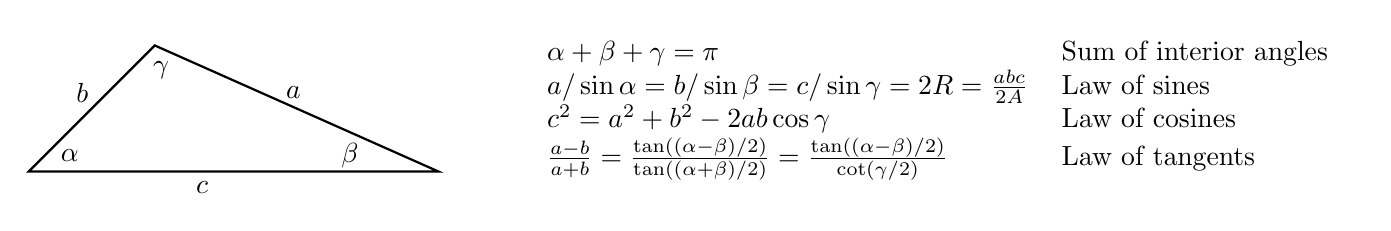
\begin{tikzpicture}[thick, scale=0.4]
\draw (0,0)--(13,0)--(4,4)--cycle;
\node at ( 1.3, 0.5) {$\alpha$};
\node at (10.2, 0.5) {$\beta$};
\node at ( 4.2, 3.2) {$\gamma$};
\node at ( 5.5,-0.5) {$c$};
\node at ( 1.7, 2.5) {$b$};
\node at ( 8.4, 2.5) {$a$};
%\node[align=left] at (17,3) {$c^2=a^2+b^2$\\ $b^2=p^2+h^2$ \\ $a^2=q^2+h^2$};
\node[align=left] at (29,2) 
{
\begin{tabular}{l l}
  $\alpha + \beta + \gamma = \pi$                       & Sum of interior angles \\
  $a / \sin \alpha = b / \sin \beta 
    = c / \sin \gamma 
    = 2R = \frac{abc}{2 A}$                             & Law of sines \\  
  $c^2 = a^2 + b^2 - 2ab \cos \gamma$                   & Law of cosines \\
  $\frac{a-b}{a+b} 
   = \frac{\tan((\alpha-\beta)/2)}{\tan ((\alpha+\beta)/2)} 
   = \frac{\tan((\alpha-\beta)/2)}{\cot (\gamma/2)}$
                                                        & Law of tangents \\
\end{tabular}
};
\end{tikzpicture}
\medskip

%\medskip
%\begin{tabular}{l l}
%  $\alpha + \beta + \gamma = \pi$                       & Sum of interior angles \\
%  $a / \sin \alpha = b / \sin \beta 
%    = c / \sin \gamma 
%    = 2R = \frac{abc}{2 A}$                             & Law of sines \\  
%  $c^2 = a^2 + b^2 - 2ab \cos \gamma$                   & Law of cosines \\
%  $\frac{a-b}{a+b} 
%   = \frac{\tan((\alpha-\beta)/2)}{\tan ((\alpha+\beta)/2)} 
%   = \frac{\tan((\alpha-\beta)/2)}{\cot (\gamma/2)}$
%                                                        & Law of tangents \\
%\end{tabular}
%\medskip
% maybe try to draw a triangle next to to the table showing all the quantities...without taking any more vertical space ...it doesn't seem to work - maybe do it in the same way as with the right triangle - include the formulas into the tikz picture - use two columns of text
% OK - done...the commented tabular environment is now inside the tikzpicture


where the quantities $R, A$ appear. These and others can be computed via:

\medskip
\begin{tabular}{l l}
 $s = (a+b+c)/2$                       & Semiperimeter, half of the perimeter \\
 $A = \sqrt{(s-a)(s-b)(s-c) s} = r s$  & Area (via Heron's formula) \\
 $r = \sqrt{(s-a)(s-b)(s-c)/s} = A/s$  & Radius of inscribed circle \\  
 $R = (abc)/ A$                        & Radius of circumscribed circle \\
 $r = \frac{s-a}{\cot(\alpha/2)}
    = \frac{s-b}{\cot(\beta/2)}
    = \frac{s-c}{\cot(\gamma/2)}$      & Law of cotangents\\
\end{tabular}
\medskip


\paragraph{More Formulas} $ $ \newline
% For some reason, we need this "$ $ \newline" nonsense to convince LaTeX to put the tabular
% on a new line

%\medskip
\begin{tabular}{l l}
 $\sin(\gamma / 2) = \sqrt{ (s-a)(s-b) / (a b)  }$      & Half-angle formula for sine \\
 $\cos(\gamma / 2) = \sqrt{ s(s-c) / (a b)  }$          & Half-angle formula for cosine \\
 $\tan( \gamma) = \frac{c \sin \alpha}{b - c \cos \alpha}
              = \frac{c \sin \beta} {a - c \cos \beta}$ & Tangent formula  \\
 $\frac{a-b}{c} 
   = \frac{\sin( (\alpha - \beta)/2) } { \sin( (\alpha + \beta)/2) }
   = \frac{\sin( (\alpha - \beta)/2) } { \cos( \gamma/2) } $
                                                        & Mollweide formula for sine \\
 $\frac{a+b}{c} 
 = \frac{\cos( (\alpha - \beta)/2) } { \cos( (\alpha + \beta)/2) }
 = \frac{\cos( (\alpha - \beta)/2) } { \sin( \gamma/2) } $
                                                        & Mollweide formula for cosine \\
 $c = a \cos \beta + b \cos \alpha$                     & Projection theorem \\  
 $H_a = b \sin \gamma = c \sin \beta$                   & Height above side $a$ \\ 
 $A = a H_a / 2$                                        & Area via height \\
 $M_c = \sqrt{2(a^2+b^2) - c^2}/2
      = \sqrt{a^2+b^2 +2ab\cos\gamma}/2$                & Length of median of side $c$ \\
 $B_{\gamma} = (2ab\cos(\gamma/2))/(a+b)
      = \sqrt{ab \; ((a+b)^2-c^2)}/(a+b)$               & Length of angle bisector of $\gamma$
\end{tabular}
\medskip


These are quite a lot of moderately complicated formulas already (you perhaps see now why we really don't want to memorize them) and by symmetry, even more formulas can be obtained by doing the cyclic replacements: $a \rightarrow b \rightarrow c \rightarrow a$, $\alpha \rightarrow \beta \rightarrow \gamma \rightarrow \alpha$. 


\paragraph{More Definitions and Facts}
A couple of terms appeared in the descriptions of the formulas above. They deserve some explanation. The \emph{perimeter} is the total length of all the sides, i.e. the length that you would have to walk if you walk around the triangle. The \emph{semiperimeter} is half of that. The \emph{median} of a side is the line segment that starts from the middle of that side and goes to the vertex that is opposed to that side. All 3 medians meet in a common point which is the \emph{center of gravity} of the triangle. The \emph{angle bisector} is a line segment resulting from drawing a line in between the two triangle sides from a vertex using half of the angle there and extending it until it hits the opposing side. All 3 angle bisectors meet in a common point which is also the \emph{center of the inscribed circle} of the triangle. The \emph{center of the circumscribed circle} is given by the point where \emph{perpendicular line segment bisectors} meet. These are lines starting at the centers of the sides in a direction perpendicular to the respective side (ToDo: is there a formula for their lengths, too? maybe draw triangle with medians, bisectors, inscribed circle, etc. Explain center of gravity as balancing point).

% see Teubner tachenbuch, page 760,764
% https://de.wikipedia.org/wiki/Projektionssatz_(Dreieck)
% todo: law of cotangents, what about centers of the incircle and circumcircle? but maybe that's for analytic geometry because it involves coordinates

% https://en.wikipedia.org/wiki/Semiperimeter
%   "appears frequently enough in formulas for triangles and other figures that it is given a
%   separate name" 
% Is this one of the reasons why pi = tau/2 also appears quite often? pi is the length of
% semiperimeter of a circle. It gives another reason to call pi the semicircle constant.

\subsubsection{Congruence Theorems}
In geometry, two shapes are said to be congruent if they can be brought into full agreement just by means of translations, rotations and reflections - fancy terms for moving, turning and mirroring. It captures the idea that the two shapes are the same, just possibly placed somwhere else in space with a possibly different orientation. There are 5 theorems that state sufficient conditions for two triangles to be congruent. Two triangles are congruent if at least one of the following statements holds true: (SSS) all three sides have matching lengths, (ASA) one side and the two adjacent angles match, (SAS) one angle and the two adjacent sides match, (AAS) two angles and one side match, (SsA) two sides and the angle adjacent to the smaller side match (the lowercase 2nd s is not a typo - it indicates the smaller side). ...ToDo: verify these, especially SsA and give the formulas/algorithms to compute the missing pieces. Explain also similarity (here, also scaling is allowed - its should preserve only distance ratios where congruence preserves distances themselves. I think it also preserves angles)

% on (SsA): https://www.jstor.org/stable/27966706

%https://tutors.com/math-tutors/geometry-help/triangle-congruence-theorems-sss-sas-asa
%https://j-tradition.com/congruence.html


\subsubsection{Right Triangles}
Of special importance are triangles in which one angle is a right angle. These are unsurprisingly and rightfully called right triangles. There can be only one right angle in a non-degenerate triangle because two right angles already sum up to a straight angle, which is also the sum of all 3 angles - so if you attempt to have two right angles, you'll get (in the limit) a degenerate triangle whose 3rd vertex is at infinity with an angle of zero (because they are parallel). By the way, triangles in which two sides have the same length are called \emph{isosceles} and those where all three sides are equal are called \emph{equilateral}. But this is just more jargon and not super important. The right triangles are the mathematically important ones. Pictured below is a right triangle with sides $a,b,c$ that is split into two further right triangles by a drawing a perpendicular from the top vertex to the base side $c$. The height of the triangle is denoted by $h$. Next to it are some relevant formulas that hold in such a situation.

\medskip
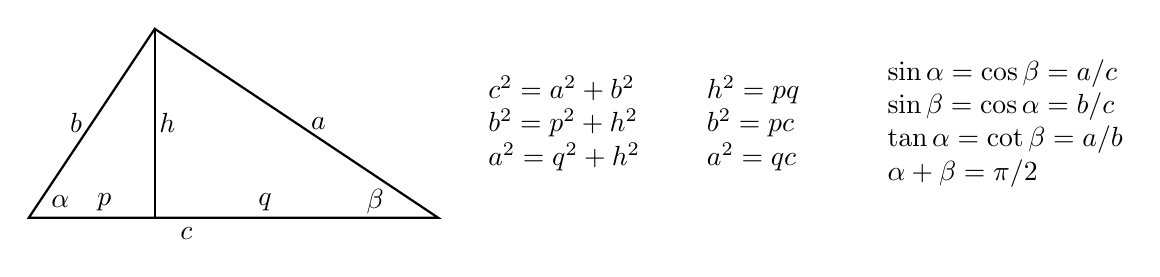
\begin{tikzpicture}[thick, scale=0.4]
\draw (0,0)--(13,0)--(4,6)--cycle;
\draw (4,6)--(4,0);
\node at (1.0, 0.5) {$\alpha$};
\node at (2.4, 0.5) {$p$};
\node at (7.5, 0.5) {$q$};
\node at (11.0, 0.5) {$\beta$};
\node at (5.0,-0.5) {$c$};
\node at (1.5,3.0)  {$b$};
\node at (9.2,3.0)  {$a$};
\node at (4.4,3.0)  {$h$};
\node[align=left] at (17,3) {$c^2=a^2+b^2$\\ $b^2=p^2+h^2$ \\ $a^2=q^2+h^2$};
\node[align=left] at (23,3) {$h^2 = p q$ \\ $b^2 = p c$ \\ $a^2 = q c$};
\node[align=left] at (31,3) {$\sin \alpha = \cos \beta = a/c$ \\ 
   $\sin \beta  = \cos \alpha = b/c$ \\ 
   $\tan \alpha = \cot \beta  = a/b$ \\ 
   $\alpha + \beta = \pi/2$};
\end{tikzpicture}
\medskip
% see Teubner Taschenbuch, page 761
% see at around 19:40 - Inverser Satz des Pythagoras: 1/a^2 + 1/b^2 = 1/h^2
% https://www.youtube.com/watch?v=od9lUVypXrQ


The $a^2 + b^2 = c^2$ relation is the famous theorem of Pythagoras which is a special case of the law of cosines when the angle $\gamma$ is a right angle in which case the cosine term vanishes ($\gamma$ is not shown - it's the angle opposite to side $c$). The two equations below are the same theorem applied to the sub-triangles. In the middle column are Euclid's altitude theorem (aka height theorem) and below are his theorems of sides. In the right column are some angle relations. [ToDo:verify everything, especially the $\cot \beta$ relation - it's just a guess from symmetry, maybe add also the converse relation for b/a] 

% https://tex.stackexchange.com/questions/29233/tikz-adding-text


%\begin{tikzpicture}[thick, scale=0.75]
%\draw (0,0) coordinate[label=below:$A$] (a) --
%      (4,0) coordinate[label=below:$B$] (b) --
%      (4,3) coordinate[label=above:$C$] (c) -- cycle;
%\end{tikzpicture}

%\include{Tikz/RightTriangle_4_3} % doesn't work - includes can't be nested - that sucks!!!

\subsubsection{More Triangle Facts}
% https://texample.net/tikz/examples/morleys-triangle/ trisectors always from an equilateral triangle

% there is a circle going through all of the 3 vertices - this is called the circumcircle and its center is called the crucumcentre

% each triangle has 3 "altitudes" (lines from one vertex going down orthogonally to its opposing side). They meet in a common point called the "Orthocentre"
% see: https://www.youtube.com/watch?v=ZrjarkXS0Fo

\subsection{Quadrilaterals}
% rant about why they are not called quadrangles or triangles not trilaterals

% see: https://www.youtube.com/watch?v=ZrjarkXS0Fo at 6:00
% -opposite angles in a cyclic quadrilateral sum to 180°  -and vice versa: if two opposite angles in a quadrilateral sum to 180, then the quadrilateral is cyclic (meaning that its 4 vertices lie on a circle) ..shouldn't that be called "circular" rather than "cyclic"

% Ptolemy’s Theorem and the Almagest: we just found the best visual proof in 2000 years
% https://www.youtube.com/watch?v=rr1fzjvqztY
% In any cyclic quadrilateral (i.e. qudrilatral inscribed in a circle). Label 2 opposite sides A,a and the tow other opposite sides B,b and the two diagonals C,c. Then: A*a + B*b = C*c. If the quadrilateral is a rectangle, we recover Pythogoras's theorem a special case.

% https://en.wikipedia.org/wiki/Semiperimeter#For_quadrilaterals

\subsection{Polygons}
% sums of interior and exterior angles, regular polygons, convexity, self-intersection


% Gauß' geniale Methode zur Flächenberechnung von Vielecken
% https://www.youtube.com/watch?v=EUAH2rSJ9Ao
% -"Schnürsenkelmethode"
% https://de.wikipedia.org/wiki/Gau%C3%9Fsche_Trapezformel
% https://en.wikipedia.org/wiki/Shoelace_formula


\subsection{Circles}

% introduce circle as 
% (1) limiting case for a regular polygon as the number of sides grows.
% (2) locus of all points at a fixed distance from some given center

% https://www.youtube.com/watch?v=rr1fzjvqztY
% 6:20: start with any chord of the circle. from the ends of the chord, draw lines that meet at the circle. all pairs of such lines will meet in the same angle at the circle
% if you also draw lines to the center of the circle, the meeting angle at the center is twice that of the meeting angle at the boundary
% when the chord goes through the center, the meeting angles at the circle's boudary are 90° (Thales theorem)

% https://en.wikipedia.org/wiki/N-sphere#Spherical_coordinates


%\subsection{Conic Sections}

%\subsection{General Shapes}
% by 2D shape, we usually mean something deescribed by a closed, non self-intersecting curve
% ..but we have already seen more general things: polygons that self-intesect, curves that 
% aren't closed (hyperbolas). We usually think of a shape 2D as something that has an area.
% That makes sense only for closed curves. When they self-intersect, we can still make sense 
% of it but the notion of area becomes a bit ambiguous - should some parts of the figure 
% count as negative area? Maybe based on the direction of winding of the edges around that
% sub-area? Consider a figure 8

\subsection{Geometric Derivations}
You may wonder, how all these formulas were derived geometrically or how one would go about deriving a formula geometrically at all. The process starts with a couple of points, lines or line segments and maybe circles and then makes use of the Euclidean axioms: we may pick any pair of points and draw a line between them, we may extend lines as we see fit, we may draw a circle centered at one of our points with a radius given by the distance between any pair of our points. In such a construction, we may then identify angles that must be equal to each other by the rules of corresponding, opposite, alternating or consecutive angles. We may identify sums of angles that must sum up to a right, straight or full angle. We may identify line segments or distance ratios that must be equal to each other. We may identify shapes that are congruent or similar to one another. All of that will give us equations. The "identification" of known geometric situations in itself requires two steps: recognition (usually by eye - like: "hey, these two triangles look similar!") and proof (usually by making geometric arguments based on known theorems - "like: they must indeed always be similar because of such and such theorem"). What exactly to do in a given situation to find such equations is a highly creative process. Look up "Dandelin Spheres" or watch 3blue1brown's "Why slicing a cone gives an ellipse" video for a nice example of such a geometric proof. [TODO: include a reference] A much simpler example is the proof that the sum of all angles in a triangle must be a straight angle...

% https://www.youtube.com/watch?v=pQa_tWZmlGs
% https://en.wikipedia.org/wiki/Dandelin_spheres

ToDo: draw the picture that shows that the angles in a triangle must sum to 180


% Explain that it is importnat to not jump to conclusions from a particluar drawing. In geometry, there often are a lot of different cases and configurations to consider and the drawn one is usually just one of them. We must make sure to really take into account all possible configurations.


% The AI that solved IMO Geometry Problems | Guest video by ‪@Aleph0‬
% https://www.youtube.com/watch?v=4NlrfOl0l8U
% -Explains computer algorithms (with and without AI) that solve geometry problems
% -Explains that geometrioc derivations often involve "auxiliary constructions" - drawing in lines,
%  circles, etc. that are not there already
% -Coming upt with such auxiliary constructions is hard - the search space of possible constructions
%  is infinite


\subsection{3D Geometry}

% angles in 3D, solid angles

\subsubsection{Platonic Solids}
% all faces, sides and angles are the same
% tetrathedron, cube, ...

\subsubsection{Polyhedra}
% Euler's formula, generalization to nD: polytopes (I think)

\subsubsection{Solids of Revolution}
% sphere (revolve a half-circle), cylinder (revolve a rectangle), cone (revolve a 
% right triangle)


\begin{comment}
	
Maybe explain why we say triangles and quadrilaterals but not, more consistently, either triangles and quadrangles or trilaterals and quadrilaterals. One suffix-term focuses on the angles, the other on the sides - I think

https://texample.net/tikz/examples/area/geometry/
http://www.tikzedt.org/

https://github.com/walmes/Tikz  examples mainly for statistics

-center circumscribed circle: intersection of medians
-center of inscribed circle: intersection of angle bisectors

https://en.wikipedia.org/wiki/Median_(geometry)
https://de.wikipedia.org/wiki/Seitenhalbierende

https://mathworld.wolfram.com/AngleBisector.html
https://en.wikipedia.org/wiki/Angle_bisector_theorem
https://en.wikipedia.org/wiki/Bisection#Triangle
https://de.wikipedia.org/wiki/Winkelhalbierende

https://mathworld.wolfram.com/PerpendicularBisector.html
https://en.wikipedia.org/wiki/Bisection#Perpendicular_line_segment_bisector
https://de.wikipedia.org/wiki/Mittelsenkrechte

https://en.wikipedia.org/wiki/Incircle_and_excircles_of_a_triangle

https://en.wikipedia.org/wiki/Mollweide%27s_formula

https://en.wikipedia.org/wiki/Law_of_cotangents

https://en.wikipedia.org/wiki/Circle

-thales' theorem

-rename file to Geo_Elementary

-plot a drawing of a triangle with vertices A,B,C, sides a,b,c and angles alpha, beta, gamma
-give a bunch of formulas that hold for all triangles
-the plot some special triangles (right, isosceles, etc.) and give the formulas specific to them
-mention non-Euclidean trigonometry, espeically spherical...maybe give the formulas for those
triangles, too - or maybe refer to some ressource

-give formulas for volumes of 3D shapes

https://en.wikipedia.org/wiki/Trigonometry

Weitz: Elementargeometrie (Vorkurs Mathematik)
https://www.youtube.com/watch?v=cMuoFr4DvDo

Weitz: Überblick Elementargeometrie: Winkel, Satz des Pythagoras, Sinus, Kosinus, etc.
https://www.youtube.com/watch?v=zVLFfgg7f98&list=PLb0zKSynM2PBYzz6l37rWH3B_n_7P40QP&index=167

How many lines go through 4 given lines in 3D?
https://www.youtube.com/watch?v=F5d8fUXf7d8
-6:40 Galucci's Theorem: 3 skew lines in 3D always define a ruling of either hyperboloid 
 or (in exceptional cases when all 3 lines are parallel to the same plane) a hyperbolic 
 paraboloid (see also: ruled surface). 
-A hyperboloid has two different rulings. A line from one such ruling intersects all lines of the
 other ruling. 
-This implies that for 3 given lines in 3D, there are infinitely many lines that intersect all 3.
-For 4 given lines on 3D, there are 4 cases: 
 1: the 4th line does not intersect the hyperboloid -> no line exists that intersects all 4
 2: the 4th line is tangent to the hyperboloid -> one line intersects all 4
 3: the 4th line pokes through the hyperboloid -> two lines intersect all 4
 4: the 4th lines lies on the same ruling of the hyperboloid -> infinitely many lines intersect 
    all 4 (namely, those on the opposite ruling)
-This is a topic of enumerative geometry and Schubert Calculus

the forgotten 3 dimensional Pythagorean theorem.
https://www.youtube.com/watch?v=vcnQ0GR4IPI
https://en.wikipedia.org/wiki/De_Gua%27s_theorem

Divine high PHI: The power of AB=A+B (Mathologer masterclass)
https://www.youtube.com/watch?v=cCXRUHUgvLI
at 6:40 - Ptolemys theorem - generalization of Pythagoras theorem

-Hint at non-Eulcidean geometries: 
 -straight lines don't exist anymore - we need to use geodesics instead
 -spherical: angle sum in triangles is > pi, ratio of circumfence to radis in circle is
  < pi, 
 -hyperbolic:
 -This will be picked up in more detail in the context of differential geometry


Red or Green: Which is larger? (Guess before you watch)
https://www.youtube.com/watch?v=xKQuEREy5fY


\end{comment}
\section{Analytic Geometry}
Analytic geometry is about representing the positions of points within space by numbers and doing calculations with these numbers. These numbers are called "coordinates" and are to be understood with respect to a given coordinate system which has to be chosen beforehand. From points, more complex objects like lines, planes, shapes, etc. can be made up and we are interested in computing things like the distance of a point from a line or plane etc.. The term "analytic" is, in my humble opinion, a bit misleading here because "analysis" is usually taken to be a more rigorous version of calculus but in analytic geometry, we typically do more basic vector- and matrix-algebra stuff and the more calculusy things are usually tackled later in "differential" geometry. However, "analytic" geometry, just like "elementary" geometry, is also mostly a bunch of formulas that are useful for creating more complex geometric algorithms. The main distinctive feature is that these formulas will typically involve representations of our shapes in terms of vectors of coordinates. This is actually the more typical representation we use in a computer, at least in the context of graphics but also for physical simulations. 

%===================================================================================================
\subsection{The $2D$ Euclidean Plane $\mathbb{R}^2$}
The simplest setting to do analytic geometry in is the $2$-dimensional plane also known as the Euclidean plane which we denote as $\mathbb{R}^2$ due to the fact that we use two real numbers to specify a location in this space. This is the place where Euclid himself developed all the geometric notions that we learn today in school. The objects we will deal with are points, lines, curves, triangles and polygons. The quantities we are interested in are distances, angles and areas. ...TBC...

%---------------------------------------------------------------------------------------------------
\subsubsection{Points, Vectors and Vertices}
Our eventual goal is to describe geometric shapes and calculate certain features of them. The most primitive object that we need to build our representations of shapes from is a \emph{point}. A point is just a location in a space - in this case, a location in the $2D$ plane. When we build polygons from points, we will also call these points \emph{vertices} (singular: \emph{vertex}) and we may use \emph{vectors} to represent these points. Conceptually, a point is actually not the same thing as a vector. A point is just a location in space and it doesn't seem to be a meaningful idea to add two locations in space together, for example. A vector, on the other hand, is meant to encode a length and direction (of movement, for example) and it does indeed make geometric sense to add a vector to a point to get another point. Vectors are things that we can freely add together anyway and the result will always be another vector. Such an addition does make geometric sense as well: we first do one translation, then the other - the sum of the two vectors encodes to total translation. Even though it doesn't make sense to \emph{add} two points, it does make sense to \emph{subtract} two points - and the result will be the vector that tells us, how to move from one point to the other. This seems all very messy. In practice, however, the distinction between points and vectors is rarely made and points are just identified with their position vectors, i.e. vectors that go from the origin of the coordinate system to the point. So, in this setup, the terms point, vector and vertex kinda all mean the same basic mathematical object, namely a vector, but the usage of different terms can be viewed as a hint to what specific role a given vector currently plays. If we say vertex, the role is typically to be a corner of a polygon. If we say point, the role is typically a general location. If we say vector, the role may be a translation or displacement. But whatever the role is, the representation will always be a pair of real numbers, i.e. a $2D$ vector.

...TBC...TODO: introduce different notations for points and vectors.

%In this context, the points are also often called "vertices" and they can be represented by vectors. 

%---------------------------------------------------------------------------------------------------
\subsubsection{Lines}
After points (or vectors or vertices), the next object we need is the \emph{line}. A line can be defined in various ways. Perhaps the most obvious way is to use two points because given two distinct points, there is always exactly one line that passes through both of them. It is noteworthy that by line, we mean the infinitely extended line that goes through the two points. If we mean just the segment of the lines in between the two points, we call it a \emph{line segment}. In the great scheme of things, lines can be viewed as $1D$ spaces in their own right - and points would be the edge case of $0D$ spaces. Let's start with two points represented via their position vectors $\mathbf{p}_1, \mathbf{p}_2$ and their difference vector $\mathbf{v}$ which encodes how to move from $\mathbf{p}_1$ to $\mathbf{p}_2$:
\begin{equation}
\mathbf{p}_1 = \begin{pmatrix} x_1 \\ y_1 \end{pmatrix}, \quad
\mathbf{p}_2 = \begin{pmatrix} x_2 \\ y_2 \end{pmatrix}, \qquad
\mathbf{v}   = \mathbf{p}_2 - \mathbf{p}_1 
\end{equation}
In this case, $\mathbf{p}_1$ and $\mathbf{p}_2$ are really playing the role of points in the sense that they encode locations whereas $\mathbf{v}$ is a proper vector in the narrower sense of encoding a displacement.

\begin{tikzpicture}
[thick, >=stealth', 
  dot/.style = { draw, fill = black, circle, inner sep = 0pt, minimum size = 4pt }
]

% Coordinate system:
\draw[->] (-5,0)  -- (10,0) coordinate[label = {below:$x$}] (xmax);
\draw[->] (0,-3)  -- (0,5)  coordinate[label = {left:$y$}] (ymax);

% Line:  
\draw     (-4,-1) -- (6,4)  node[pos=0.9, below right] {Line};

% Points on the line:  
\draw (2,2) node[dot, label = {above:$\mathbf{p}_1$}]{};
\draw (4,3) node[dot, label = {above:$\mathbf{p}_2$}]{};

% Marks on the x- and y-axes:
\draw (2,0) node[dot, label = {below:$x_1$}]{};  
\draw (4,0) node[dot, label = {below:$x_2$}]{};
\draw (0,2) node[dot, label = {left:$y_1$}]{};
\draw (0,3) node[dot, label = {left:$y_2$}]{};
% ToDo: try to use tick-marks instead - or just drop horizontal and vertical lines

\end{tikzpicture}
% adapted from:
% https://texample.net/tikz/examples/linear-regression/

..TBC..give different forms of a line and formulas to convert between them, formulas for angles, distance point-line, projection of points onto lines, ...

% points can be seen as 0D objects, lines as 1D

% Leupold, pg 174-176:
% 3.44:  m = tan(alpha) = (y2-y1)/(x2-x1)     Anstiegswinkel
% 3.45:  r = r1 + t*(r2 - r1)                 Parameterdarstellung
% 3.46:  r = r1 + t * u                       u = r2-r1
% 3.47:  (y-y1)/(x-x1) = (y2-y1)/(x2-x1)      Zweipunkteform, (2-point form?)
% 3.48:  y-y1 = m*(x-x1)                      Punktrichtungsform
% 3.49:  y = m*x + b                          Normalform, (explicit?)
% 3.50:  x/a + y/b = 1                        Abschnittsform
% 3.51:  Ax + By + C = 0                      allgemeine Form
%
% m: slope, a: x-intercept, b: y-intercept, r1 = (x1,y1), r2 = (x2,y2)

% Leupold

%---------------------------------------------------------------------------------------------------
\subsubsection{Curves}

%---------------------------------------------------------------------------------------------------
\subsubsection{Triangles}


%---------------------------------------------------------------------------------------------------
\subsubsection{Polygons}


%---------------------------------------------------------------------------------------------------
\subsubsection{Conic Sections}

\paragraph{Circles and Ellipses}

\paragraph{Hyperbolas}

\paragraph{Parabolas}




%ToDo: representation as 2D vectors, points, lines, formulas for: distance between points, between point and line, angle between lines, ...


%===================================================================================================
\subsection{The $3D$ Euclidean Space $\mathbb{R}^3$}
When we up our game by one dimension from the Euclidean plane, we arrive at the $3$-dimensional Euclidean space. Points, lines, triangles and curves are still a thing - but they will now exist in $3$ rather than $2$ dimensions. But we also get a new type object to deal with: arbitrary planes. In the $2D$ case, there was \emph{the} plane which was the backdrop for all the objects. Now planes themselves are objects within the larger $3D$ space and they can have any orientation within that larger space. We even get curves surfaces which was also not a thing in $\mathbb{R}^2$. Polygons can still make sense in $\mathbb{R}^3$, but we need to be a bit more careful because it's not guaranteed anymore that all the vertices of a polygon lie in the same plane. This was not an issue in $2D$ space. ...TBC...

%ToDo: representation as 3D vectors, points, lines, planes, formulas for: distance between point and line, point and plane, intersection point of line with plane, intersection line of 2 planes, intersection point of 3 planes, angle between plane and line, plane and plane, ...


%===================================================================================================
\subsection{The $nD$ Euclidean Space $\mathbb{R}^n$}
Having seen the Euclidean spaces of dimension $2$ and $3$, it's now time to generalize to Euclidean spaces of arbitrary dimension. ...TBC...

%\subsection{The Euclidean }

%---------------------------------------------------------------------------------------------------
\subsubsection{Lines}
Given a point $\mathbf{p}$ and a nonzero vector $\mathbf{v}$, both elements of $\mathbb{R}^n$, we can consider the following set of points:
\begin{equation}
 L 
 =
 \{\mathbf{p} + \mathbb{R} \mathbf{v} \} 
 = 
 \{ \mathbf{p} + t \mathbf{v}, \; t \in \mathbb{R} \}
\end{equation}
This set of points represents a line in $\mathbb{R}^n$. The expression in the middle is just a shorthand notation for the expression on the right. Multiplying the vector $\mathbf{v}$ by the set of real numbers $\mathbb{R}$ is meant in the sense that we take $\mathbf{v}$ and multiply it by every possible real number $t \in \mathbb{R}$. This line $L$ goes through the point $\mathbf{p}$ and has a direction of $\mathbf{v}$. The line is given in the so called \emph{parametric form}\footnote{Well, I think, for a parametric form, one would more commonly write out a separate equation for each coordinate if $n$ is known and small enough like $2$ or $3$. For general unknown $n$, this vector form can be seen as a more abstract way of writing down a parametric form.} with the parameter $t$. It's also called the \emph{vector form}. We can imagine that, as $t$ sweeps through the real numbers, a point sweeps along the line. For each value of $t$, we obtain some point on the line by just plugging the value $t$ into the formula. With $t=0$, we are at $\mathbf{p}$. With $t=1$, we are at $\mathbf{p + v}$. With $t=\frac{1}{2}$, we are at $\mathbf{p} + \frac{1}{2} \mathbf{v}$ which is exactly halfway between $\mathbf{p}$ and $\mathbf{p + v}$. And so on. The vector form is not the only way to define a line. One can also use two (distinct) points $\mathbf{p}_1,\mathbf{p}_2$ on the line and two real numbers $t_1, t_2$ that satisfy $t_1 + t_2 = 1$ and express the line as the set of points:
\begin{equation}
 L = \{ t_1 \mathbf{p}_1 + t_2 \mathbf{p}_2,  \quad t_1, t_2 \in \mathbb{R}, t_1 + t_2 = 1 \}
\end{equation}
This is called a \emph{two point form}. It may also be called a representation in terms of \emph{barycentric coordinates}, although that terminology is less commonly used for lines - it's more commonly used for planes that are defined by 3 points or $n$-dimensional hyperplanes that are defined by $n+1$ points, but it is the proper $1D$ analog. You may wonder why we introduce the variable $t_2$ and don't just use $1 - t_1$ instead (and then drop the index altogether). The reason is that this would work only for the 1D case, i.e. the line, but writing it like above will readily generalize to barycentric representations of higher dimensional objects. Yet another way to define a line is by means of an implicit equation of the form...TBC....TODO: give other forms of a line (implicit, explicit, etc.), mention that it can be generalized from $\mathbb{R}^n$ to vector spaces over any field - the complex numbers are interesting in the context of algebraic geometry, give the ways to convert between the different forms.

% Two lines are parallel, when they have parallel direction vectors. Two vectors are parallel when one is a scalar multiple of the other

% https://en.wikipedia.org/wiki/Line_(geometry)#Definition
% https://en.wikipedia.org/wiki/Barycentric_coordinate_system

% https://math.stackexchange.com/questions/2931233/the-vector-form-and-parametric-forms-of-a-line-given-a-point-and-direction-or

%---------------------------------------------------------------------------------------------------
\subsubsection{Planes}
Given a point $\mathbf{p}$ and two linearly independent\footnote{Linear independence implies that both must be nonzero.} vectors $\mathbf{v, w}$, consider the following set of points:
\begin{equation}
 \mathbf{p} + \mathbb{R} \mathbf{v}  + \mathbb{R} \mathbf{w}
 \quad = \quad
 \mathbf{p} + s \mathbf{v} + t \mathbf{w}, \; s,t \in \mathbb{R}
\end{equation}
This set of points represents a plane in $\mathbb{R}^n$. 

%---------------------------------------------------------------------------------------------------
\subsubsection{Hyperplanes}
After having seen lines and planes, the pattern continues. We can take some fixed point $\mathbf{p}$ together with a set of $k$ linearly independent vectors $\mathbf{v}_1, \mathbf{v}_2, \ldots, \mathbf{v}_k$ and consider the set:
\begin{equation}
 \mathbf{p} + \sum_{i=0}^{k} t_i \mathbf{v}_i, \; t_i \in \mathbb{R}
\end{equation}
This set defines a $k$-dimensional hyperplane in $\mathbb{R}^n$ where $k < n$. Well, we could perhaps allow $k=n$ as edge case as well, but then we would just get the whole space $\mathbb{R}^n$ and that's not interesting. We are interested in substructures of $\mathbb{R}^n$. But $k > n$ does really not make any sense at all, not even as edge case, because then we can't even find a set of $k$ linearly independent vectors anymore.

% https://web.evanchen.cc/handouts/bary/bary-short.pdf

%---------------------------------------------------------------------------------------------------
%\subsection{Quadrics}

% https://en.wikipedia.org/wiki/Quadric_(algebraic_geometry)
% Maybe do it in algebraic geometry








\begin{comment}


Geometrische Interpretation linearer Abbildungen
https://www.youtube.com/watch?v=EQ5Xct2YyLk


Weitz: Analytische Geometrie
https://www.youtube.com/watch?v=7rkkHIjHtNI
https://www.youtube.com/watch?v=7rkkHIjHtNI&list=PLb0zKSynM2PBYzz6l37rWH3B_n_7P40QP

\end{comment}
\section{Algebraic Geometry}
Algebraic geometry investigates the sets of zeros of multivariate polynomials and the geometrical shapes that are defined by these zero sets. Consider as example the bivariate polynomial $f(x,y) = x^2 + y^2 - r^2$ for some given constant $r$. Those points $(x,y)$ in the $xy$-plane for which this function produces zero as output define a geometric shape - in this case, a circle of radius $r$ centered at the origin. You can have multiple simultaneous equations that must be equal to zero and of course, you can also have more than two input variables. It's also possible to consider complex solutions, in fact, that's the more typical setting. In general, these sets of solutions to polynomial equations are called "algebraic varieties" and these are the main subject of interest in algebraic geometry.

\medskip
It is also possible to work in the field of rational numbers $\mathbb{Q}$ rather than in the field of complex numbers $\mathbb{C}$ or even in finite fields such as $\mathbb{Z}_p$ for a given prime number $p$. ...TBC..

\medskip
Fun fact: algebraic geometry and geometric algebra are two fields of mathematics that have nothing to do with each other. Isn't that weird? I really wonder, how connections between these fields could look like. Maybe we could start by interpreting the variables in the equations as multivectors instead of real or complex numbers? I have no idea but I think there just \emph{should} be some connection!




%===================================================================================================
\subsection{Algebraic Varieties}
An \emph{algebraic variety} is the set of solutions to a system of polynomial equations $f_1(\mathbf{x}) = 0, \ldots, f_m(\mathbf{x}) = 0$ where $\mathbf{x} = (x_1, \ldots, x_n)$ and the $f_i$ are multivariate polynomials, i.e. polynomials with $n$ input variables that we may collect in an input vector $\mathbf{x}$ whenever this is notationally convenient. In general, this set of solutions is a set of points in an $n$-dimensional space. The dimensionality of the variety will typically be given by $n-m$ where $n$ is the number of variables and $m$ the number of equations [VERIFY!]. ...TBC...

% ACRS uses multisets to define varieties. This is done to deal with repeated components of the curve or variety. The book doesn't use the term "variety" and instead talks about "hypersurfaces". Funny enough, it nonetheless uses the letter V for the "hypersurface" without explaining for what that V is supposed to stand. I have a hunch.

%---------------------------------------------------------------------------------------------------
\subsubsection{Parameterizations}
Defining a shape as the solution set of a system of equations is also called an \emph{implicit definition}. Sometimes it is more convenient to have a more explicit representation of the set of points. A fully explicit representation would be, if we could isolate one variable and express it explicitly as function of all the others. But requiring such a functional representation is often too restrictive - there are some shapes that simply cannot represented that way. For example, we could try to represent the circle explicitly as $y = \sqrt{r^2 - x^2}$ but that would give us only the upper half the circle unless we interpret the square-root as multi-valued function, which is already inconvenient in this very simple toy example and in more complicated cases, things may get out of hand even more. If a fully explicit representation is not possible or practical, the second best thing is to let all the coordinates be functions of a set of some auxiliary variables which we call parameters. In the case of a circle, that could look like $x(t) = \cos(t), y(t) = \sin(t)$ for $t \in [0, 2 \pi]$. In such a representation we call $t$ the parameter.
...TBC...

\paragraph{Finding Rational Parameterizations}
The parameterization of the circle via the cosine and sine functions given above is not the only possible way to parameterize the circle. It will probably be the most common one in most practical contexts (such as computer graphics) but from an algebraic point of view, it has a flaw: it requires usage of transcendental functions. Wouldn't it be much nicer in an algebraic context if we could use purely algebraic functions to parameterize it? We can and in fact, we need only rational functions - not even roots are needed. I will give a recipe to find a rational parameterization of the unit circle that can sometimes be used for other curves as well. We proceed as follows:

%To find a rational parameterization of an implicitly given curve, we sometimes can proceed as follows:

...TBC...

% https://en.wikipedia.org/wiki/Circle#Parametric_form

% https://people.reed.edu/~jerry/131/conics.pdf
% explains how the rational parameterization of the unit circle is related to the standard substitution t = tan(x/2) in intergrals of rational functions in sin(x), cos(x), etc.

% this too:
% https://en.wikipedia.org/wiki/Tangent_half-angle_substitution

\paragraph{From Parameterization to Equation}
Now we look at the inverse problem: We assume that we have a rational parameterization given and we ask what the corresponding implicit equation is. ...TBC...

% circle: ACRS, pg 2, general: 68 - has also algorithm for the inverse problem

% important questions: find a (rational) parameterization, is the zero set a manifold? what topological invariants does it have?

% Bezout's Theorem


% https://en.wikipedia.org/wiki/Algebraic_variety
% https://mathworld.wolfram.com/AlgebraicVariety.html



%---------------------------------------------------------------------------------------------------
\subsubsection{Examples}

\paragraph{Circles, Spheres and Hyperspheres}
As a simple example, consider 2D space and the single equation $x^2 + y^2 - 25 = 0$. This equation defines a circle of radius $5$ centered at the origin of the $xy$-plane. If we look at 3D space, we could define a sphere of radius $r$ via the polynomial equation in 3 variables $x^2 + y^2 + z^2 - r^2 = 0$. Note that the set of points that satisfies this equation is only the surface of the sphere, not the full ball. So, the dimensionality of the set of points that satisfies this equation is 2, not 3. 

\paragraph{Conic Sections}
A circle is defined by a bivariate polynomial of degree 2, i.e. a quadratic polynomial. The circle is therefore also called a curve of degree 2 or quadratic curve. Besides the circle, all conic sections, i.e. sets of solutions of equations of the form $0 = A x^2 + B y^2 + C x y + D x + E y + F$, fall into this category. They are called conic sections because these shapes also arise from intersecting a cone with a plane.

\paragraph{Elliptic Curves}
The set of solutions of $y^2 = x^3 + a x + b$ for some given values $a,b$ is called an "elliptic curve". These are not to be confused with actual ellipses, which are special cases of conic sections. Rather, elliptic curves represent a canonical form of the generalization of conic sections up to degree 3 (verify!).



\paragraph{Torus}

%simple examples: cassini curves, lemniskate, torus

% AVRS, pg 72: 
% -Nodal cubic curve: y^2 = x^2 + x^3
% -Folium of Descartes: x^3 + y^3 = 3 x y

% https://en.wikipedia.org/wiki/Lemniscate
% https://de.wikipedia.org/wiki/Lemniskate
% https://en.wikipedia.org/wiki/Polynomial_lemniscate

% -Give implicit equation and parametrization(s) whereever possible and if possible also an explicit
%  formula




%---------------------------------------------------------------------------------------------------
\subsubsection{Problematic Intersection Points}
Consider the situation where we have two polynomial equations $f(x,y) = 0$ and $g(x,y) = 0$ in 2D and we want to find all the intersection points of the two curves that are defined by the two polynomials respectively. Such intersection points can be found by solving the equation $f(x,y) = g(x,y)$ for pairs $(x,y)$ that satisfy the equation. For simplicity, let's assume that $g(x,y) = ax + by + c$, i.e. $g$ is only of degree one such that defines a straight line. In an ideal world, we would like to see exactly $n$ intersection points between the curve $f$ and the line $g$ if the polynomial $f$ has degree $n$. We can indeed make that (and more) work by tweaking the problem setting appropriately whenever we encounter a problematic situation in our current setting.

\paragraph{Intersections at Complex Coordinates}
At first, we assume that our "current setting" takes place in the usual Euclidean $xy$-plane which we also call $\mathbb{R}^2$. If we take $f(x,y) = x^2 + y^2 + 1$ and $g(x,y) = 0$, we can easily convince ourselves that no pair $(x,y)$ will ever satisfy the equation $x^2 + y^2 + 1 = 0$. Except when we allow $x$ and $y$ to be complex valued. In that case $x = 0, y = \i$ would work, for example. So, our first tweak to the problem setting setting is that we move it from $\mathbb{R}^2$ to $\mathbb{C}^2$. This will not solve all of our problems but it gets us some way into the right direction.

% -solution: use the field of complex numbers

\paragraph{Intersections at Infinity}
A second problem that we may run into is exemplified by the following situation: let $f(x,y) = 2 x - y + 1$ and $g(x,y) = 2 x - y + 2$. These define two parallel lines that obviously intersect nowhere - not even when $x$ and $y$ are allowed to be complex. The solution to this problem is, informally, that we "add points at infinity" and say that two parallel lines intersect at such a point at infinity ...TBC...

% -solution: consider also intersections at infinity

\paragraph{Multiplicities of Intersections}
Consider $f(x,y) = x^2 - y$ and $g(x,y) = y$. If we draw the curves defined by setting each equation individually to zero, we will draw the parabola $y = x^2$ for $f$ and the horizontal line $y = 0$, i.e. the $x$-axis, for $g$. These two curves do not intersect but rather touch at $(x,y) = (0,0)$. The straight line $g$ is tangential to the parabola $f$ at this point. Such points of tangency highlight yet another problem that we might run into.
 ...TBC...

% perturb g a bit - shift it a bit up - the point of tangency turns into two points of intersection. In general, in teh complex domain, we will see higher order saddles so we will get more intersection points by such a perturbation when there is a higher "order of tangency" (verify!)

% -tangency, tangetial intersections or rather touching points
% -solution: count intersections with multiplicity

%===================================================================================================
\subsection{Projective Space}
What we informally and vaguely called "adding points at infinity" will now be fleshed out for real. The idea is to go from the normal $n$-dimensional vector space to a so called \emph{projective space}. This is a space with $n+1$ dimensions and the vectors in this space do not represent points in the $(n+1)$-dimensional space but rather lines through the origin. Each vector in the projective $(n+1)$-space is interpreted as being just a representative of a whole equivalence class of vectors consisting of all scalar multiples of that vector. Vectors or points in the original $n$-dimensional space are recovered by considering the intersections of these lines with a specific (hyper-) plane - namely the one for which the extra dimension has a value of one. 

% https://en.wikipedia.org/wiki/Projective_space
% https://en.wikipedia.org/wiki/Projection_(mathematics)#Central_projection

\subsubsection{Homogeneous Coordinates}
The way to realize this projective space is to switch to so called \emph{homogeneous coordinates}. To get a feeling for how that works, let's start with our usual Euclidean plane $\mathbb{R}^2$. We'll actually eventually apply the idea to $\mathbb{C}^n$, but imagining to start with $\mathbb{R}^2$ is okay for intuition building and this intuition happens to be also practically relevant for computer graphics. The points in our original space $\mathbb{R}^2$ are given as pairs $(x,y)$. What we now do is to add an extra coordinate which we call $w$ such that our points are now given as triples $(x, y, w)$. If $w \neq 0$, then these triples will encode the point $(x/w, y/w)$ in our original space [VERIFY!]. If $w=0$, they kind of still do represent $(x/w, y/w)$ but since $w = 0$, these points will be "at infinity" - and it's not just any infinity but an infinity that lies ahead in a specific direction, namely into the direction of the vector $(x,y)$. In some sense, we have added directional infinities to our space. We can envision these points as lying on a perimeter of a circle with infinite radius such that this perimeter is infinitely far away. But there's a catch: diametrically opposite points on this infinite circle are identified with one another - the infinity to the right is the same as the one to the left (and may just be called the horizontal point at infinity). The mental picture is that we "wrap-around" at the (directional) infinities. This is the 2D version of the way we think of the projectively extended real number line (see \cite{WK_ProjExtReals}) with its single added point at infinity. The fact that we encode a 2D vector $(x,y)$ by a triple $(x,y,w)$ by saying that we get our 2D vector back via $(x/w, y/w)$ implies that the "encoding" of a given finite $(x,y)$ vector is not unique. For example, the triple $(15,12,3)$ encodes the same 2D vector as the triple $(5,4,1)$, namely the 2D vector $(5,4)$. It turns out that for $w \neq 0$, we can always normalize our triple in such a way that $w=1$: We simply divide all 3 components by whatever $w$ currently is. The subset of $\mathbb{R}^3$ for which $w = 1$ is the horizontal plane, parallel to the $xy$-plane at a $w$-height of $1$. Our $(x,y,w)$ triples really represent lines through the origin of $\mathbb{R}^3$ and the intersection points of these 3D lines with the $w=1$ plane in 3D space determine the $(x,y)$ coordinates of our point in the original 2D space. To distinguish coordinate tuples in the projective space from those in an ordinary vector space, some authors denote the vectors using colons instead of commas as in $(x : y : z)$ instead of $(x, y, z)$. We will adopt this practice along with the convention of using the letter $w$ for the extra coordinate which we will always put last into the extended coordinate tuple as in $(x : y : w)$ or $(x : y : z : w)$. Some authors put the extra ("$w$") coordinate first. The colon is supposed to hint at a division by $w$ which is what we will have to do to recover our coordinates in the original $n$-space as we will see. That makes me think that $(x,y,z : w)$ might be an even better notation - but I'll stick to the established one. There is another caveat: We have said that the homogeneous coordinate vector $(x : y : w)$ stands for the vector $(x/w, y/w)$ in ordinary coordinates and we have said that if $w=0$ and $x$ and $y$ are nonzero, it stands for the point at infinity into the $(x,y)$ directions (both ways - forward/backward). But what if $x$ and/or $y$ are also zero? Actually, the case that they are both also zero is disallowed: the triple $(0:0:0)$ is not a valid homogeneous coordinate vector. But something $(0:3:0)$ is allowed and it seems to indicate that we need to compute $0/0$ for the $x$-coordinate of the ordinary vector. But we do not really need to compute an $x$-coordinate because we are dealing with a point at infinity which has no $x$-coordinate. Points at infinity do not really have coordinates in the usual sense - they only have directions. Our vector could only potentially have a direction component into the $x$-direction. But this particular infinite point hasn't one. The triple $(0:3:0)$ represents the two points at infinity into the purely vertical directions. The general rule is: whenever $w=0$, the represented point is at infinity and remaining components give the direction of the infinite point - except when they are all zero, which is not allowed. [VERIFY!]

% -Explain that the homogeneous tuple $(0:0:0)$ is not allowed.
% -Explain what happens in a case $(0,y,0)$ (which is allowed) to the 0/0 expression for recovering the x-coordinate in 2D space

% explain the notation (x : y : w)

%give a sort of 2D projection
%...TBC... 


% https://en.wikipedia.org/wiki/Homogeneous_coordinates
% https://en.wikipedia.org/wiki/Extended_real_number_line
% https://en.wikipedia.org/wiki/Projectively_extended_real_line


% Explain why the space is called "projective". When w != 0, we may normalize the triple wo w=1. We can interpret the w=1 plane as a slice of xyw-space and if we cut out this slice, we get our original xy-plane back. ACRS gives a "projection function" pi - but this is *not* a function that projects 3D vector onto a 2D plane. To the contrary: it "projects" 3D vectors (i.e. points) onto the embedding 3D lines in the sense of turning the points into these lines. This is a different use of the word "projection". Normally, when we "project" something, we lose one or more dimensions. We usually "project" a 3D point onto a 2D plane or similar. But here we "project" a 3D point onto/into a 3D line. Figure out how other authors use the term projection in this context! This is confusing!

% Explain how the projective space is really the space of all lines through the origin in a space one dimension higher than the original space. The *normalized* (n+1) tuples can be identified with the w=1 plane and the coordinates in R^n space are obtained by intersecting the lines with that plane.

\subsubsection{Homogeneous Polynomials}
When we are working with homogeneous coordinates, we give the space one extra coordinate. We use $(n+1)$ dimensional space but we still want to use polynomials to describe shapes in $n$-dimensional space by way of zero-sets of polynomial equations. That puts some constraints on the kinds of polynomials that we can use for this purpose. In 2D, if $(x : y : 1)$ is a point such that $p(x,y,1) = 0$, we'd better make sure that this occurs if and only if $p(x/w, y/w, w) = 0$ for any $w$ we may choose. Otherwise the shape would not be well defined. The way we ensure this is called homgenization. We take our original polynomial in $x,y$ and multiply each monomial in it by an appropriate power of $w$ such that each monomial has the same total degree. Being homogeneous is indeed the property that we need to satisfy our constraint, because if a multivariate polynomial $f(\mathbf{x})$ is homogeneous of degree $n$, then we have $f(k \mathbf{x}) = k^n f(\mathbf{x})$ for any input multiplier $k$, so in particular, $f(k \mathbf{x}) = 0$ whenever $f(\mathbf{x}) = 0$ [VERIFY!].

...TBC...

%If a polyno

%===================================================================================================
\subsection{Elliptic Curves}

\subsubsection{Elliptic Curves} 
% asterisk means: can be skipped on first reading
Here, we will consider a certain subset of bivariate polynomial equations that turned out to be in the sweet spot between being enough to actually tackle them and complex enough to allow for some interesting features. I'm talking about the so called elliptic curves. But didn't we already talk about ellipses as one particular type of conic section? Yeah - an \emph{elliptic curve} is actually \emph{not an ellipse} but rather the set of solutions of a bivariate polynomial equation of degree 3. ToDo: explain etymology if the term

\paragraph{$\star$ Group Structure} % star means: can be skipped on first reading
The set of rational points on such an elliptic has an interesting property: together with a suitably defined binary operation between these points, they form an algebraic structure known as commutative group. That basically means that we can plug two rational points into our operation and the operation will produce another rational point on the curve. In the context of elliptic curve theory, this operation is usually denoted  with $+$ and called addition - but it is \emph{not} just the regular vector addition. ...TBC...
% see Elliptic Tales, pg 116
% mention that i works also when we don't work over Q but over a finite field
% The points on the elliptic curve




\subsection{$\star$ The Abstract Perspective}
This section can be skipped on a first reading of the book. It references rather advanced ideas that are properly introduced only (much) later - specifically \emph{ring theory} from abstract algebra.




\subsubsection{Polynomial Rings}
Algebraic geometry, when viewed as the business of trying to find the set of solutions of multivariate polynomial equations, is actually about quite intuitive ideas. However, when you open a textbook on algebraic geometry written for real mathematicians, you will discover that it will talk about very abstract ideas that sound like they have nothing to do with geometry. In the abstract algebra perspective of algebraic geometry, we consider quotient rings of polynomial rings. For example, in 2D, when we have a bivariate polynomial like $p(x,y) = x^2 + y^2 - 1$, we will consider the ring $R = \mathbb{R}[x,y] \setminus (x^2 + y^2 - 1)$ and analyze its properties with the arcane machinery of ring theory. ...TBC...

% Is this the ring of all polynomials that are zero on p? Or is it the ring of all polynomials
% but we are allowed only to plug in values for which p(x,y) = 0 i.e. only points on the unit
% circle?
% Our ring $R$ is the ring of all polynomials $q(x,y)$ that

% What is algebraic geometry?
% https://www.youtube.com/watch?v=MflpyJwhMhQ
%
% -Maybe this chapter should have a last section: Ring Theoretic Perspective or similar which 
%  can be skipped on a first reading
%
% -Maybe bring a 1D example: take a polynomial like p(x) = (x+2)*(x-3) = x^2 - x - 6 with 
%  roots at {-2,3}
% -Consider the ring R[x] \ p(x)
% -It is the ring of all polynomils that has zeros at -2,3. The set of all these polynomials
%  is considered to form an eqivalence class.
% -Any polynomial that is zero at -2 and 3 must have p(x) as factor, so any polynomial with p
%  as factor is considered to be equivalent...right...or wrong?

%
% -Or is it like we we consider the ring of all polynomials but we allow only to plug in 
%  points (x,y) for which the polynomial is zero?



\begin{comment}



https://de.wikipedia.org/wiki/Algebraische_Geometrie
https://de.wikipedia.org/wiki/Algebraische_Variet%C3%A4t
https://de.wikipedia.org/wiki/Hilbertscher_Basissatz
https://de.wikipedia.org/wiki/Gr%C3%B6bnerbasis

https://en.wikipedia.org/wiki/Algebraic_geometry
https://en.wikipedia.org/wiki/Algebraic_variety

https://en.wikipedia.org/wiki/Zero_of_a_function#Zero_set
https://en.wikipedia.org/wiki/Projective_plane

https://en.wikipedia.org/wiki/Rational_mapping

https://en.wikipedia.org/wiki/Elliptic_curve
https://en.wikipedia.org/wiki/Algebraic_curve
https://en.wikipedia.org/wiki/Weierstrass_elliptic_function


https://en.wikipedia.org/wiki/K3_surface
https://en.wikipedia.org/wiki/Calabi%E2%80%93Yau_manifold

https://en.wikipedia.org/wiki/Duality_(projective_geometry)

-conic sections in 2D and 3D, classification
-elliptic curves
-lemniskate, contour plots
-polynomials with integer/rational coeffs -> integer and rational solutions -> elliptic curve cryptography
-what about allowing more general classes of functions?
-what about multiple simultaneous equations - what does that imply for the dimensionality of the solution set?
-what are important features of the solution sets? connectedness?

-seems like differential geometry deals with parameteric representations and algebraic geometry with implicit representations of geometric shapes (manifolds?)
-is there a way to convert between these representations? ..yeah...this seems to be actually a difficult research area

Tikz:
https://texample.net/tikz/examples/feature/angles/
https://texample.net/tikz/examples/feature/foreach/

https://pbelmans.ncag.info/blog/2010/11/11/howto-draw-algebraic-curves-using-pgftikz/

-write a c++ function that takes in an implicit function f(x,y) = 0 and spits out a vector of vectors of 2D points (the outer vector is because we may have multiple curves), this can then be converted into svg or tikz code (via suitable code-generators that take as input the coordinate vectors)
-with this code, generate tikz figures for elliptic curves, maybe x^2 + y^3 + k = 0 for different values of k

Fun fact

Wie muss man fragen, um "schöne" Antworten zu bekommen? (Der Satz von Bezout):
https://www.youtube.com/watch?v=dyehHqozzqE




\end{comment}
\section{Differential Geometry}
In algebraic geometry, we considered zero sets of systems of polynomial equations. Under certain circumstances, these zero sets define a manifold and sometimes, we could find a parametric representation of such a manifold, i.e. a formula, that takes as input one or more independent parameters and spits out a point on the manifold as output. Differential geometry (DG) typically takes a parametric representation, i.e. a vector valued function of possibly multiple arguments, of such a manifold as a starting point. Since we will need to take work with (partial) derivatives of such a parametric representation, we will assume that all the functions are differentiable sufficiently often.

\medskip
DG can be roughly split into "classical" or "elementary" DG and "modern" DG. The former deals with curves in the 2D plane and with curves or surfaces in 3D space and is typically expressed in (a subset of) the language of vector calculus. The latter deals with the completely general case of $kD$ manifolds in $nD$ space where $k \leq n$ and is typically expressed in (a subset of) the language of differential forms (aka exterior calculus) and/or tensor calculus. Important applications of classical DG are in computer graphics, modern DG features prominently in general relativity.

\medskip
A very important, maybe the most important, concept in DG is the idea of curvature.

% curves vs surfaces vs general manifolds, intrisic vs extrinsic

...tbc...



\begin{comment}
	
In algebraic geometry, we deal with a manifold that is defined by an implicit equation of the form f(x,y) = 0 in 2D or f(x,y,z) = 0 in 3D or a system of such equations like f(x,y,z) = 0, g(x,y,z) = 0 in 3D. The equations are assumed to be polynomials but (I guess) the general ideas can be generalized to arbitrary equations. The manifold is typically of a dimensionality given by the dimensionality of the embedding space minus the number of equations (verify!). When I say "typically", I mean that there may be other cases but these can be considered as somehow being degenerate edge cases (verify!). For example, if we have have 1 equation in 3 variables, we normally get a 2D manifold, i.e. a surface in 3D space. 

In differential geometry, we also deal with manifolds but here, the manifolds are not defined via an implicit equation but rather by a set of parametric equations. We can imagine the parametrization to define a map of the manifold. We may have different parametrizations (i.e. maps or charts or patches) for different regions. The totality of all these maps (i.e. the set of all the maps) is called an atlas. Ideally, the maps should cover the whole manifold. Different maps may overlap with respect to the region that they cover. If they do overlap, they should agree in the regions of overlap. ...tbc...

In some sense, algebraic geometry is simpler than differential geometry because it just involves solving algebraic equations. Differential geometry, on the other hand, uses a lot of calculus which is usually considered to be a more advanced math topic than algebra. But in some other ways, differential geometry might also be considered easier that algebraic geometry because in DG we have the luxury of getting a parametrization of our manifold handed to us on a silver plate. Such a parametrization is for many purposes a much more convenient description of the manifold than the unwieldy implicit equation that AG gives us. One could actually say that the availability of the parametrization \emph{enables} us to make use of a lot of calculus that would unavailable otherwise.

differential: local properties such as curvature, metric tensor, gradient, tangential plane/space
algebraic: global properties such as number of holes, orientability, number of stationary points, number of
 self-intersections, winding number

https://mathworld.wolfram.com/Atlas.html
https://en.wikipedia.org/wiki/Atlas_(topology)#Charts

ToDo:
-There are at least 2 ways of defining a surface in 3D: 
 -parametrically as x(u,v), y(u,v), z(u,v) - that's the DG approach
 -implicitly as F(x,y,z) = 0 - that's the AG approach
-An explicit form z = f(x,y) can be seen a special case of both:
 parametric: x(u,v) = u, y(u,v) = v, z(u,v) = f(u,v)
 implicit:   F(x, y, f(x,y)) = 0
-Explain, how we can get a local parametrization from an implicit equation using
 partial derivatives...I'm not sure, if that's possible but I think, it should be.
 See:
 https://tutorial.math.lamar.edu/classes/calciii/parametricsurfaces.aspx
-Maybe we could also try to convert locally to an explicit form. It would become locally
 a 1D root-finding problem of F(x,y,z) = 0. Here, x,y are plugged in and can be seen as 
 parameters and we want to find z.
-Explain how we may get an implicit form from a given parametrization
-Sochi's book says that DG is more concerned with local features of the manifolds whereas
 AG is more about global features.
-I think, the fundamental local feature in DG is the metric tensor. Most other quantities of
 interest can be derived from it. In the case of surfaces, the metric tensor is just a 2x2 
 matrix. It can be computed from the extrinsic description of the surface via its 
 parametrization but one often just assumes it to be *somehow* given without caring much about 
 the how. It is an intrinsic feature of the manifold that can also be measured from an observer 
 who lives inside the manifold (Like A. Square living in flatland). Derived quantities are
 the different forms of curvature (except geodesic curvature which is an extrinsic property), 
 the Christoffel symbols, etc.
-Global features are things like the number of stationary points, orientability, presence or 
 absence of self-intersections, topological features such as the genus, ...

-Maybe use a circle of radius 5 as example curve and represent it 
 parametrically: c(t) = (5 cos(t), 5 sin(t))
 implicitly:  x^2 + y^2 - 25 = 0
 explicitly: y = +- sqrt(25 - x^2)
 and compute the tangent vector at a point (say (4,3)) via all 3 representations. Investigate, 
 how we can, from a given implicit equation and a point on the curve, compute coordinates of 
 another (infinitesimally) nearby point. Parametric and explicit representations can be used
 straightforwardly to "generate points" - but how can the implicit equation be used for that?
 1: by considering it a root-finding problem, 2: by assuming that we have a point given and
 somehow obtain a nearby point? ..which we may or may not refine using a root-finder?

%An Amazing Theorem for Tangents (Fabricius-Bjerre Theorem)
%https://www.youtube.com/watch?v=7_UclB2dB0o

Differential Geometry: The Intrinsic Point of View #SoME3
https://www.youtube.com/watch?v=jWoyBlIXVd8
-Gaussian curvature, being the product of two extrinsic quantities (namely, the two principal
 curvatures), turns out to be an intrinsic property. That's what Gauss found remarkable, according
 to this video. The "Theorema Egregium" itself is of a more quantitative nature, though.
-The Riemann curvature tensor is the nD generalization of Gaussian curvature.


https://en.wikipedia.org/wiki/Lie_derivative

How mathematicians describe curvature of surfaces
https://www.youtube.com/watch?v=UYiAlYlSwBo

What is Differential Geometry?
https://www.youtube.com/playlist?list=PLXo8Tdaw0czOWyRD-esa6mNajlPZnjHQs


Lisa Piccirillo: Exotic Phenomena in dimension 4
https://www.youtube.com/watch?v=BXwALAkPubc

How to Get to Manifolds Naturally
https://www.youtube.com/watch?v=lEX4kSB5CAI

How to do Calculus on an Abstract Manifold
https://www.youtube.com/watch?v=pNlcQ0Tx4qs


the geometry of the third derivative
https://www.youtube.com/watch?v=h4kGXlKz5GI



https://www.youtube.com/watch?v=o8swNKLHDzo  How to describe Curvature?
-5:44: for a triangular region:  sum-of-angles - 180° = integral over Gaussian curvature
 ...but I guess the 180° must be re-expressen in radians?
-7:02: sufaces with zero mean curvature are minimal surfaces
 Q: is the converese also true?


Differential Geometry in Under 15 Minutes
https://www.youtube.com/watch?v=oH0XZfnAbxQ
-Nice overview - also explains Stokes' Theorem in terms of differential forms

Why Distances Depend on the Geometry You Live In
https://www.youtube.com/watch?v=5qAvXdBTISo

The Core of Differential Forms
https://www.youtube.com/watch?v=DOPwupMCcUs
-A 1-form is a generalization of a directional derivative. It takes a vector as input and
 produces a scalar as output

How to Describe an Entire Space with a Matrix
https://www.youtube.com/watch?v=bt7Msd1b5VA
-about the Ricci curvature tensor (a symmetric rank 2 tensor)
-it quantitfies how geodesics bend together or drift apart 
-this can also be understood in terms of how hypervolumes expand when we move outward from a point
-nD generalization of the 2D concept of Gaussian curvature (?) ...or rather maybe a generalization
 of the principal curvatures?
-defined as contraction of Riemann curvature tensor (rank 4 tensor)
-

But what are manifolds, anyway? (Explained at 5 levels of difficulty)
https://www.youtube.com/watch?v=OdWaYWtrZI4
-Very nice and intuitive explanation

Manifolds
https://www.youtube.com/watch?v=aDzX6rsALy0


\end{comment}
%\section{Fractal Geometry}



\begin{comment}

-Fractals can be defined via 
 (1) line-drawings (Hilbert curve, dragon curve) vs defined as 
 (2) of some region (Mandelbrot set, Julia set)
 (3) algorithmically (Sierpinsi triangle)
-(1) is connected to curves in differential geometry - we define a curve via a function f: R -> R^2
 (2) is more like algebraic geometry - we define a set by a property: S = {(x,y) \in R^2 : ...}
 (3) like elementary geometry - start with triangle, duplicate, scale, move, etc.
-I thinlk, (2) can also be formulated in terms of (discrete) dynamical systems. There are also 
 fractals arising from continuous dynamical systems, I think.
-Self similarity
-Fractal Dimension
-Space filling curves


\end{comment}
%\include{Geo_Discrete} % but maybe this should got into the discretet math part
% maybe the geometry chapte should go into the applications part

\chapter{Functional Analysis}
Functional analysis studies operations that take a function as input. As output, these operations may produce another function in which case they are called operators, or just a simple number in which case they are called functionals. Some simple examples of operators, operating on a function $f$, are: take the derivative of $f$, take an antiderivative, multiply the input function $f$ by some (fixed) other function $g$. An example for a functional $F$ that just produces a number as output would be to take the definite integral of $f$ over some given interval $(a,b)$. An even simpler, nonetheless practically very relevant, example of a functional $F(f)$ of a function $f = f(x)$ is to just extract the value of $f$ at a given $x$, for example at $x=0$, so we would just have $F(f) = f(0)$. In any case, we are one level higher up the ladder: we are now talking about functions-of-functions, so to speak. Especially in computer science, such higher level function-like objects are also sometimes called functors. 

\paragraph{}
Functional analysis plays an important role in the study of differential equations. An ordinary differential equation (ODE), for example, may take a "driving function" as input (i.e. as right-hand-side, inhomogeneity) and produce as output a solution function which can be interpreted as the "response" of a system for the given input function. In such a context, we may in practice have to deal with driving functions that are not necessarily differentiable or even continuous - but when dealing with differential equations, we often really need to be able to take derivatives. That's one reason why a generalized notion of function-like objects, called distributions, is introduced. For these distributions, we have a notion of differentiation that is always applicable - even in the case of discontinuous functions. This notion will help us to find solutions to ODEs even for such discontinuous driving functions which we otherwise just couldn't handle properly. A strange object, called the Dirac delta-distribution $\delta(x)$, will play an important role in this context. It can be thought of as a "function" that is zero everywhere except at $x=0$ where it is infinite in such a way that the integral over any interval that includes $x=0$ equals unity. It represents an inifinitely narrow impulse of unit energy concentrated at $x=0$. No classical function behaves in such a bizarre way. If we know the response of a linear ODE to such an impulse, we can compute the response to any driving function as superposition of such impulse-responses. This superposition will be a continuous one, given by an integral, called the convolution integral.

\paragraph{}
In the context of boundary value problems and/or partial differential equations (PDEs), this notion of an impulse response will be generalized to what is called a Green's funcion...tbc...

\paragraph{}
An important type of operators are integral operators, prominent examples of which are given by the Fourier- and Laplace transform. These transforms take functions from one space (the time domain) to another (the frequency domain) and in this new space, the complicated process of convolution can be replaced by a simple pointwise multiplication. Moreover, the frequency domain is more intuitive for human interpretation - we may identify perceptually important features of signals often more easily in the frequency domain, especially in the case of audio signals.
..tbc...

\paragraph{}
In multivariable calculus, we have already seen concepts from linear algebra and calculus merge to produce new, hybrid objects like vectors and matrices of partial derivatives like the gradient vector and the Jacobian and Hessian matrices. In functional analysis, these two important fields of mathematics also come together, but this time in a very different way: Certain sets of functions will be equipped with some more structure on the set so as to form vector spaces. This additional structure may contain linear-algebra'ish things like norms of functions, scalar products between functions, linear mappings of functions to other functions, etc. These mappings often involve calculusy things like taking derivatives or integrals. These function spaces, i.e. vector spaces whose elements/vectors are functions, will often be infinite-dimensional which is a qualitative difference to the finite-dimensional vector spaces we have seen before. Nonetheless, we'll see a lot of analogies. Let's get started!

\begin{comment}


-integral transforms (fourier- and laplace trafo)
-greens-functions
-calculus of variations
-operators: eigenvalues, eigenfunctions


\end{comment}
\section{Function Spaces}
Recall from linear algebra the general definition of a vector space as a set of elements, called vectors, that can be added together to give another vector or multiplied by a scalar (i.e. a number) to give another vector. Now notice that we can do these two things with functions just the same: adding two functions pointwise gives a perfectly valid other function and multiplying a function by a number also gives another bona fide function. It can be easily verified that all the required vector-space rules such as associativity, commutativity, distributivity, neutral elements, etc. are satisfied for these operations, when applied to functions. That means, we can actually view the set of all real-valued functions $f: \mathbb{R \rightarrow R}$ as a vector space! This vector space, however, has a fundamentally different nature than those we have seen before. In order to uniquely determine a function $f$, we will have to say what its function value will be for any given input value $x$. If the domain of the function is the whole real number line (or even just a finite interval of it), that means, we must prescribe (uncountably) infinitely many function values, so the dimensionality of the space of all functions that map real numbers to real numbers is apparently also (uncountably) infinite. We will also encounter subspaces of this huge space whose dimensionality will be only countably infinite or even just finite.

\subsection{Scalar Products}
In the $N$-dimensional vector space $\mathbb{R}^N$, the standard scalar product of two vectors $\mathbf{u,v}$ was defined as the sum over the element-wise products:
\begin{equation}
 \langle \mathbf{u,v} \rangle = \sum_{i=1}^{N} u_i v_i
\end{equation}
That motivates the definition of the scalar product of two real-valued functions $f,g$, both defined on some interval $(a,b)$, by analogy as:
\begin{equation}
 \langle f,g \rangle = \int_a^b f(x) g(x) \; dx
\end{equation}
This is one possible definition of a scalar product on a space of functions and it is in fact the one that is most often used, but there are some other variations that should be mentioned, too. ...
% introduce the general from with a weight and maybe also the complex form, maybe also with a positive definite kernel, what about the integration limits, there are also scalar products involving derivatives

\subsection{Norms and Distances}
In $\mathbb{R}^N$, the Euclidean norm of a vector was defined as the square root of the scalar product of the vector with itself. We can define a norm for functions in a completely analogous way. However, we don't necessarily need a scalar product to define a norm. Another way to define a norm would be to just take the maximum value of the function within a given interval. ...
% L_p-norm, maximum-norm, norms induced by a scalar product, distances (norms of differences)

\subsection{Special Function Spaces}
Often we are not interested in the vast and unstructured set of all possible real functions but only in a subset of it, i.e. in a set of functions that meet some additional criteria. We may, for example, demand that the functions have to be continuous, differentiable, (square-)integrable, bounded, periodic, monotonic, symmetric, etc. It turns out that many of these subsets are actually also subspaces in the sense that addition of two such functions or multiplication of one of them by scalar will always give a new function that also belongs to the set. Some of these specific function spaces are important enough that they have been given special names, so we shall now familiarize ourselves with this terminology.

\subsubsection{Continuity and Differentiability}
One way to categorize functions is by considering, how smooth they are. Does a function $f$ have spikes, jumps, corners, etc? That idea is captured by the number of continuous derivatives that a function has. If a function is $k$ times continuously differentiable, then it is said to be in the class $C^k$. If a function is just itself continuous but has a discontinuous first derivative, it is in the class $C^0$ but not in the class $C^1$. An example of such a $C^0$ but not $C^1$ function would be the absolute value $f(x) = |x|$. In general, the classes with lower $k$ are less restrictive, i.e. allow more functions. But the classification is meant in an inclusive sense, i.e. a function that is in $C^k$ is automatically also in $C^j$ if $j < k$. If a function can be differentiated $k+1$ times, it means that the $k$-th derivative is not only continuous but even differentiable which is a stronger requirement. That means, a function that can be differentiated $k+1$ times is automatically at least in $C^k$. If a function can be differentiated infinitely often, it is said to be in the class $C^\infty$. Such functions are also called \emph{smooth}. If, in addition to be infinitely differentiable, it also has a convergent Taylor series at every point of its domain, it said to be in $C^\omega$ and also called \emph{analytic}\footnote{The letter $\omega$ is also used in other areas of math (ordinal numbers, nonstandard analysis) to denote "infinity". I'm not sure, if that usage there is related but to be honest, I can't see how. It seems like the $\omega$ from ordinal numbers would mean exactly the same thing as the $\infty$ symbol as it is used here. So maybe drawing a connection would be a bit hasty.}. Analytic functions are in some sense even nicer than just smooth ones.

%...TODO: define $C^k$ spaces including $C^\infty$ and $C^\omega$

% Bump functions are in  $C^\infty$ but not in $C^\omega$. Explain why!

% https://en.wikipedia.org/wiki/Smoothness
% https://mathworld.wolfram.com/C-kFunction.html

\subsubsection{Integrability} Functions can also be categorized according to their integrability. By analogy with the classification based on differentiability, you might guess that we consider repeated integration of a function. But that's not how it works. Instead, we consider the integral of the $p$-th power of the absolute value of the function. For example, for functions $f: \mathbb{R} \rightarrow \mathbb{R}$, we may consider the integral of the absolute value of $f$ over the whole domain: $\int_{-\infty}^{+\infty} |f(x)| \; dx$ and classify those functions for which this integral is finite as belonging to the class of \emph{absolutely integrable} functions over the real numbers. Next, we may introduce an exponent $p$ to whose power we raise the absolute value and look at $\int_{-\infty}^{+\infty} |f(x)|^p \; dx$ and requiring that integral to be finite. For the special case $p=2$, we call the class of functions \emph{square integrable} and for general $p$, we call the functions \emph{$p$-th power integrable}. Generalizing further, we may consider functions $f: \mathbb{R}^n \rightarrow \mathbb{R}$ and look at $\int_{\mathbb{R}^n} |f(x_1, x_2,\ldots,x_n)|^p \; dx_1 dx_2 \ldots dx_n$ and requiring that integral to be finite. Generalizing even further, we may consider functions from any set $S$ for which a measure $\mu$ is defined into the real numbers\footnote{I guess, it could be generalized even further to allow the codomain be any set $T$ on which a suitable absolute value function is defined. $T =\mathbb{R}$ or $T = \mathbb{C}$ are two obvious choices.} $\mathbb{R}$ such that $f: S \rightarrow \mathbb{R}$ and requiring $\int_S |f|^p \; d \mu $ to be finite. This integral is apparently meant to be understood as a Lebesgue integral - so we require that the $p$-th power of the absolute value of $f$ must be Lebesgue integrable and the integral must be finite. We denote this set of functions by $\mathcal{L}^p(S,\mu)$ and call it the set of \emph{measurable functions} [VERIFY!]

%When talking about measures, it is clear


%any set of objects $T$ on which an absolute value is defined (such as $T =\mathbb{R}$ or $T = \mathbb{C}$)

% The normed vector space ( L p ( S , μ ) , ‖ ⋅ ‖ p ) {\displaystyle \left(L^{p}(S,\mu ),\|\cdot \|_{p}\right)} is called L p L^{p} space or the Lebesgue space of p p-th power integrable functions

%This idea could be generalized to functions $f: \mathbb{R}^n \rightarrow \mathbb{R}$ by considering $\int_{\mathbb{R}^n} |f(x_1, x_2,\ldots,x_n)|^p \; dx_1 dx_2 \ldots dx_n$ and requiring that integral to be finite.

%That is, for some given $f$, we consider the integral $\int_S |f|^p \; d \mu$ where $S$ is some set on which $f$ is defined (i.e. a subset of the domain of $f$) and $\mu$ is some measure that is defined on $S$ [VERIFY].

% https://en.wikipedia.org/wiki/Lp_space#Lp_spaces_and_Lebesgue_integrals

%\begin{equation}
%\int_S |f|^p \; d \mu
%\end{equation}

%Rather than considering repeated integration (as we did in the case), we consider

%TODO: define $L^p$ spaces named after Lebesgue, explain $\mathcal{L}^p, \ell^p$

% https://en.wikipedia.org/wiki/Lp_space#Lp_spaces_and_Lebesgue_integrals

% https://en.wikipedia.org/wiki/Lp_space
% https://en.wikipedia.org/wiki/Absolutely_integrable_function
% https://en.wikipedia.org/wiki/Square-integrable_function
% https://mathworld.wolfram.com/SquareIntegrable.html

% https://de.wikipedia.org/wiki/Lp-Raum

% https://en.wikipedia.org/wiki/Measurable_function
% https://mathworld.wolfram.com/MeasurableFunction.html


\subsubsection{Normed Function Spaces}
Let's go back the expression $\int_{-\infty}^{+\infty} |f(x)|^p \; dx$ that defines the class of $p$-th power integrable functions $f: \mathbb{R} \rightarrow \mathbb{R}$ by the requirement that this integral must be finite. So far, we really only looked at the cases $p=1$ and $p=2$. We initially intended to let $p$ be a positive natural number but we now want to widen our perspective to allow real $p \geq 1$ and even allow for $p = \infty$. In order to get nice behavior when we let $p$ go to infinity, we will now look at the expression $(\int_{-\infty}^{+\infty} |f(x)|^p \; dx)^{1/p}$. As long as we were just concerned with the finiteness of the integral and $p$ was assumed to be a finite positive number, it didn't really matter whether or not we do the $(\ldots)^{1/p}$ step at the end. But for what we want to do now, namely defining a norm that is still meaningful when $p \rightarrow \infty$, we need this additional reciprocal exponent\footnote{At least, I think this is the reason why we formerly left out the $p$-th root. Consider what happens to the integral expression when $p \rightarrow \infty$: for $|f| < 1$ the integrand will go to zero and for $|f| > 1$ the integrand will go to infinity. It appears like taking the $p$-th root after integration tames this behavior and we get a meaningful limit when $p \rightarrow \infty$.}. We define the $p$-norm of a function $f: S \rightarrow \mathbb{R}$ as
\begin{equation}
 \norm{f}_p = \left( \int_S |f|^p \; d\mu \right)^{1/p}
\end{equation}


 ...TBC...TODO: introduce $p$-norm and $L^p$ spaces as space of equivalence classes of functions from an $\mathcal{L}^p$ space

% https://en.wikipedia.org/wiki/Norm_(mathematics)#p-norm

% https://web.archive.org/web/20201024063542/http://faculty.bard.edu/belk/math461/LpFunctions.pdf

\paragraph{Banach Space}

\paragraph{Hilbert Space}

% https://en.wikipedia.org/wiki/Lp_space#Special_cases
% L^2 is the only Hilber space among the L^p spaces

\paragraph{Sobolev Space}


%\subsubsection{Analytic Functions}
% Smooth Functions, Differentiable Functions
%\subsubsection{Square Integrable Functions}
% finite support

%\subsubsection{Polynomials}
% powers, power series, orthogonal sets of polynomials (Legendre, Chebychev, etc.)

%\subsubsection{Periodic Functions}

% Hilbert-/Banach-/Sobolev-spaces, maybe drag the "Test Functions" subsection to here - it may fit here even better, maybe after analytic functions - maybe use the order: analytic, test, square-integrable as Weitz in his video about distributions

% https://en.wikipedia.org/wiki/Banach_space
% https://en.wikipedia.org/wiki/Hilbert_space
% https://en.wikipedia.org/wiki/Sobolev_space

\begin{comment}

-what are the function spaces that have a countably infinite dimension? Maybe those functions whose Taylor
 series converges everywhere belong to it
-scalar-product, norm, 
-say something about functions \mathbb{R^M \rightarrow R^N}$ - how does these fit into these scheme
-what about functions defined only on the integers or rationals?
-what about complex functions - in particular, how does the scalar product generalize

-completeness: after a norm and therefore a distance was defined, we may define Cauchy sequences of functions which are sequences of functions whose elements get arbitrarily close together with respect to the defined distance. if the limit of such a sequence also belongs to the function space, the space is said to be complete. give an example of an incomplete space and its completion...maybe the space of rational functions? could be a nice analogy to the rational numbers. consider the sequence of "Butterworth" functions f_n(x) = 1 / (1 + x^n). their limit is a step function which is not a rational function and therefore not in the set (note that the discontinuity itself is not the problem here - rational functions can be discontinuous, too due to the presence of poles - but poles are actually a different kind of discontinuity)

-norm equivalence: two norms are equivalent, iff each Cauchy sequence that converges with respect to one norm also converges with respect to the other norm and vice versa

important named function spaces:
Banach: complete, normed
Hilbert: Banach, where norm is induced by an inner product 
Sobolev: Hilbert, where differentiation is always allowed (all alements are differentiable)

\end{comment}
\section{Functionals} 

\subsection{Test Functions}
For the following material, we will need to work with a set of functions with some special properties. We want them to be smooth, which means they should be differentiable infinitely often everywhere. We also want them to have a finite support, which means they should be identically zero everywhere except within some finite interval $(a,b)$. This interval is assumed to be fixed and the same for each of the functions within the set. [VERIFY! Nope! I think, that's wrong!] The set of all functions that satisfy these two requirements will be called the set of "test functions". . At first glance, it may be a bit surprising that functions that satisfy both of these criteria even exist (it certainly suprised me). To make a function identically zero outside a given interval typically requires a piecewise definition and such piecewise definitions tend to make the functions non-smooth at the junctions of the pieces. However, such smooth, piecewise-defined functions do indeed exist, and a standard example is the so called bump function:
\begin{equation}
f(x) = 
 \begin{cases}
 \exp \Bigl( \frac{1}{x^2-1} \Bigr)  \qquad &  |x|   <  1 \\
 0                                   \qquad &  |x| \geq 1
 \end{cases}
\end{equation}
It is indeed infinitely often differentiable everywhere, even at the potentially problematic junctions at $-1$ and $+1$. It is, however, not analytic there: a power series expansion centered at these points will not converge to the function $f$.

% https://en.wikipedia.org/wiki/Bump_function
% https://en.wikipedia.org/wiki/Spaces_of_test_functions_and_distributions
% https://en.wikipedia.org/wiki/Schwartz_space

% ToDo:
% -Maybe move eplanation of test functions move to function space (it is an example of such a
%  function space). But maybe it's more appropriate to keep it here. We'll see.
% -explain where the name "test function" comes from
% -show smoothness of bump function
% -show that the Taylor series of the bump function around -1 and +1 does not converge to the
%  function. Figure out to what it converges, if at all (maybe to the zero-function?).
% -Plot the bump function. Maybe try to make a small plot next to the formula. Maybe that would be
%  a nice general way to do it throughout the book - it would be space efficient. There's typically
%  a lot of whitespace around formulas anyway


\paragraph{Notation}
As mentioned above, the set of functions that are continuous on a given interval $(a,b)$ is denoted as $C(a,b)$ and the set of functions that are continuously differentiable $k$ times on $(a,b)$ is denoted as $C^k(a,b)$. A smooth function is continuously differentiable infinitely often, so here $k = \infty$ and hence the set of smooth functions on $(a,b)$ is denoted as $C^{\infty}(a,b)$. Finally, the set of smooth functions that are zero outside the interval $(a,b)$, i.e. the set of our test functions, is denoted as  $C_0^{\infty}(a,b)$.
% Maybe do not regurgitate this stuff! Just explain the new thing:  $C_0^{\infty}(a,b)$
%or should we use brackets [] instead of ()?

% ToDo:
% Explain interpretation of test functions as weighting functions in a weighted average.


\subsection{Distributions}
In general, a dual space $V^*$ with respect to a given vector space $V$ is defined as the set of all linear functions that take as input an element of the set $V$ and spit out a scalar, i.e. a (typically real) number. What we want to define here is the space that is dual to the space of our test functions. This is the space of all linear functionals that take as input a test function and produce a real number as output. Elements of this set are called distributions and in a certain sense, they can be seen as a generalization of the idea of a function. 

% https://en.wikipedia.org/wiki/Distribution_(mathematics)

% Point out that we should not confuse the term distribtuion used here with the usage in probability theory. It's a different condept. But maybe there is some connection between the two? Figure out!

\subsubsection{Regular Distributions}
One way to construct such a linear functional is to multiply the input (test) function $f$ with some fixed other function $g$ and integrate the product over the interval $(a,b)$ over which our test function $f$ is nonzero\footnote{Which is obviously equivalent to integrating from $-\infty$ to $\infty$}. Let's call the resulting functional $G$, so we have:
\begin{equation}
 G(f) = \int_a^b g(x) f(x) \; dx
\end{equation}
% does the order of f and g matter? could we be dealing with a non-commutative multiplication?
The so constructed functionals are what we will call \emph{regular distributions}. If we identify the functionals with the functions that induce them (i.e. here, identify $G$ with $g$, assuming $a,b$ are fixed once and for all), we have a space that looks a lot like a function space, i.e. a vector space, whose elements are functions. However, the space of functionals can contain also more general objects, i.e. functionals that are not induced by a function via such an integral. A simple example of such a functional could be to just take $f$ and spit out the value of $f$ at some given fixed $x_0$. This also does everything we would expect from a functional: take a function as input, spit out a number. It is linear, too. We will call this functional a distribution, too - but it's not a regular one anymore because it's not defined by our integral construction. Instead, it's called a \emph{singular} distribution.

% claude.ai says that these are called singular distributions.
% Here are some more singular distributions:
% https://claude.ai/chat/710cfb21-fc76-4a6f-934b-a246230f9fd8

% Q: what do we need to assume about g? does it need to be square-integrable, for example? or will any arbitrary function do?

% Maybe mention that the integral may, in general, be understood as Lebesgue integral because the
% theory applies also to function which are not Riemann integrable (I think)

\subsubsection{Evaluating Distributions} ...TBC...ToDo: Explain that for distributions, it doesn't make sense (in general) to ask what value they have at a given point. 

% Instead, we are only allowed to ask questions about what the integral above evaluates to for a given test function $f$. We can "test" the distribution $g$ with $f$, where $f$ may be localized (I guess) but we cannot ask for the value of $g$ at a specific $x$. So, "evaluating" a distribution amounts to testing / probing it with a test function? Maybe that is the reason for the term distribution? We are not allowed to evaluate the function *at* a point but we are only allowed to evaluate a (weighted) average *around* a point - that is: we can figure out how the function values are "distributed" around that point? Could that even hint to a connection to probability distributions? ...or more like: probability density function? 

% ToDo:
% -explain equality of distributions and its relation to weak equality of functions - I think:
%  -Two (regular) distributions G and H are equal, if they produce the same value of the integral
%   given above for *any* (test) function f
%  -Two functions g and h are weakly equal if their associated regular distributions are equal
%  -weakly equal functions may differ from one another in isolated points as long as their values
%   are finite in these points
%  -This notion of weak equality establishes an equivalence relation of the set of (suitable)
%   functions
%  -Maybe define a symbol for weak equality - maybe a variation of the equals sign. Maybe with
%   subscript w or maybe with a w above the sign. Or maybe use the symbol that is commonly used for
%   equivalence realtions - maybe the tilde?

\subsubsection{The Dirac Delta-Distribution}
One very important example of such a singular distribution is the Dirac delta distribution that just maps any given function $f$ to its value at $x = 0$:
\begin{equation}
 D(f) = f(0)
\end{equation}
If we would try to define this distribution $D(f)$ via an integral over a product of $f(x)$ with some fixed function $\delta(x)$ as we did above for the regular distributions, we would formally get something like this:
\begin{equation}
\label{Eq:DiracDeltaDesired}
 D(f) = f(0) = \int_a^b \delta(x) f(x) \; dx
\end{equation}
and now we would ask ourselves, how the hypothetical function $\delta(x)$ would have to look like to make this work (spoiler alert: there is no such function). We would need to construct a function $\delta(x)$ which for any function $f$, when their product is integrated over an interval $(a,b)$ (which we assume to contain zero, i.e. $a < 0 < b$), gives the value of $f$ at zero. Let's try something that almost works: Pick a small positive number $\epsilon$, at least small enough such that the interval $(-\epsilon, \epsilon)$ is completely contained in $(a,b)$. Then define $\delta_{\epsilon}$ as:
\begin{equation}
\delta_{\epsilon} (x) = 
\begin{cases} 
 \frac{1}{2 \epsilon} \qquad & |x|   <  \epsilon \\
 0                    \qquad & |x| \geq \epsilon
\end{cases} 
\end{equation}
% 1/(b-a) for |x| < epsilon, 0 otherwise. It's a rectangular impulse of height 1/(b-a). Integrating delta_epsilon from a to b (or, equivalently, from -epsilon to epsilon) gives 1
Because we assumed that the interval $(-\epsilon, \epsilon)$ is completely contained in $(a,b)$, the integral of $\delta_{\epsilon}$ from $a$ to $b$ would be equivalent to the integral from $-\epsilon$ to $\epsilon$ because outside that smaller interval, the function is zero anyway. The value of the integral would be exactly $1$ because the width of the integration interval is $2 \epsilon$ and the height (i.e. the function value) is constantly $\frac{1}{2 \epsilon}$ such that the area computed by the integral is just the area of a rectangle with width $2 \epsilon$ and height $\frac{1}{2 \epsilon}$. When we would use $\delta_{\epsilon}$ in place of $\delta$ in an integral such as the one in equation (\ref{Eq:DiracDeltaDesired}) above, the output would not be exactly $f(0)$ as we would like it to be but it would be close. Specifically, it would be the average value of $f$ over a small interval (of width $2 \epsilon$) centered around zero. If we assume $f$ to be nice enough (i.e. continuous), then the smaller we take $\epsilon$, the closer the \emph{average around} zero will be to the actual \emph{value at} zero, so the better our approximation will get. If we now imagine to let $\epsilon$ approach zero, it may actually work out. The average value \emph{around} zero will certainly approach the value \emph{at} zero when the averaging interval approaches zero. However, letting  $\epsilon$ approach zero will let $\delta_{\epsilon}$ approach a nonsensical function: it approaches a function that is zero everywhere except at $x=0$ where its value is infinite. Infinity, however, is not a real number and we cannot really meaningfully treat it as such. Paul Dirac and with him the whole physics community nevertheless use this limiting "function" anyway and very successfully so. This "function" $\delta(x)$ is the (in)famous Dirac delta function. In practice (e.g. physics), it usually works well enough to think about this strange object $\delta(x)$ as a bizarre function-like object resulting from a limiting process over perfectly reasonable functions such as $\delta_{\epsilon}(x)$. In theory (rigorous mathematics), one has to accept, that a Dirac "function"  $\delta(x)$ does not really exist as such and it makes only sense to talk about the Dirac distribution $D(f)$ as a functional which is not defined via an integral. We shall take the practical point of view and pretend that $\delta(x)$ exists as a function. If it's good enough for Dirac, it's good enough for me! In the literature, the distinction between "delta-function" and "delta-distribution" is blurred and the two terms are often used interchangably and you will also find notations like $\delta(f)$ for what I have denoted here as $D(f)$. I did this to make explicit the distinction between the (non-existent) function $\delta$ and the (indeed existent) functional $D$ that $\delta$ would induce, if it would exist.

% todo: sifting property, unit-integral porperty, applications
% in precisely such a way that the integral of the whole function is unity for any integration interval that contains zero

% Couldn't we define the delate function as an actual funtion from the reals to the hyperreals?
% There, a weighted infinity is actually a thing. We could say: \delta(0) = \omega or something.

% see here:
% https://www.youtube.com/watch?v=zJk4yuzJU3s
% Demystifying the Dirac Delta - #SoME2
% -Dirac measure
% -Riesz-Markov-Kakutani theorem

% When functions have no value(s): Delta functions and distributions
% https://math.mit.edu/~stevenj/18.303/delta-notes.pdf  
% -Very well writtrn lecture notes. It's like a tutorial.
% -Has an example for when one cannot exchange limits and differentiation. Maybe that example could
%  be brought up int the Differentiation section

\subsubsection{Distributional Derivatives}
One of the motivations to develop this theory was to make sense of situations where we need to take derivatives, for example in differential equations, but the functions we have to deal with are not necessarily differentiable in the usual sense. What we want is a generalization of the derivative that is applicable to a wider class of functions or function-like objects. This wider class is the set of distributions. Remember that our plain old functions can be identified with the regular distributions which are a subset of all distributions. A distribution, seen as a functional, is completely defined by its input/output relation: if we know what it does to any input function $f$, i.e. which output number it produces, we know everything there is to know about the functional. Let's revisit our definition of a regular distribution $G(f)$, which was defined via an integral over a product of $f$ and some inducing function $g$, and see what happens, when we take the derivative $g'$ of $g$ instead of $g$ itself inside this integral. Let's call the resulting functional $G'$:
\begin{equation}
 G'(f) = \int_a^b g'(x) f(x) \; dx
\end{equation}
Now let's assume, $g$ is actually some nasty, non-differentiable function such that $g'$ makes no sense. We can nevertheless make sense of $G'$ by moving the prime in $g'$ over to $f$. What allows us to do this is the rule for integration by parts:
\begin{equation}
 \int_a^b g'(x) f(x) \; dx = \Big[g(x) f(x)\Big]_a^b - \int_a^b g(x) f'(x) \; dx
\end{equation}
Now there's no $g'$ anymore in the right hand side. Instead, we have to differentiate $f$ and that will never pose a problem to us because $f$ was assumed to be a test function, so it's differentiable infinitely often. For test functions, we also we have $f(a) = f(b) = 0$ which makes the boundary terms vanish. So, what remains is:
\begin{equation}
 G'(f) = - \int_a^b g(x) f'(x) \; dx
\end{equation}
So, we may compute the functional $G'(f)$ for any test function $f$ even for a non-differentiable inducing function $g$ by simply moving the prime from $g$ to $f$ and prepending a minus sign. This motivates the following definition of the \emph{distributional derivative}:
\begin{equation}
  G'(f) = -G(f')
\end{equation}
The distributional derivative is also called the \emph{weak derivative}. ...TBC...
% give general formula for the n-th distributional derivative using the scalar-product notation

% The distributional derivative is also called the weak derivative

% todo: consider as example f(x) = |x| and give the expressions for some of its distributional derivatives. the 1st will be a scaled and shifted Heaviside function, the 2nd will be a scaled dirac delta function, etc.

% introduce the scalar-product alike notation for the dual pairing of distributions and tes functions

% https://de.wikipedia.org/wiki/Schwache_Ableitung
% https://de.wikipedia.org/wiki/Distribution_(Mathematik)
% -Räume schwach differenzierbarer Funktionen sind die Sobolev-Räume. Ein noch allgemeinerer Begriff der Ableitung ist die Distributionenableitung

\paragraph{Example: Derivative of $|x|$}
To see our new tool in action, consider the absolute value function $f(x) = |x|$. We can write down the derivative as:
\begin{equation}
f'(x) = 
 \begin{cases}
 -1 \qquad  x < 0 \\
 +1 \qquad  x > 0
 \end{cases}
\end{equation}
But note that this doesn't say anything about $f'(x)$ at $x = 0$. We can't assign a value there because $f(x) = |x|$ not differentiable at $x = 0$ in the usual sense. But it is differentiable in the weak sense. The derivative given above has only values for $x \neq 0$. But that is no problem if we view $f'$ as a distribution. Distributions are not supposed to have values everywhere - or anywhere at all, for that matter. All that we want from a distribution is to test it with a test function. We do not generally expect to be able to evaluate it a an arbitrary point in the sense of asking: "What's your value there?". If we can, that's a bonus but it's not required. ...TBC...explain the Heaviside step function - if shift and scale $f'$ above appropriately and arbitrarily define the value at zero to 1, we obtain it.

%Note that for the weak derivative

\subsection{Weak Form of Differential Equations}

% We only care about weak equality between LHS and RHS, i.e. equality "under the averaging integral" rather than exact pointwise equality

% Maybe the subsection should be named Applications and may we can list some more. ODEs (The right hand side could be a Dirac delta), PDEs (The initial condition could be non-differentiable - like a triangular shape - maybe even a Dirac spike), embedding discrete probability distributions into the continuous framework (by placing scaled Dirac deltas at the integers, for example), modeling point masses and infinitely short hammer strikes in physics.

\begin{comment}

-Frechet-derivative: derivative for functionals - is this similar to a directional derivative? nah! that's the gateaux derivative
https://en.wikipedia.org/wiki/Fr%C3%A9chet_derivative
https://en.wikipedia.org/wiki/Gateaux_derivative
...maybe the gateaux derivative can be introduced in the context of functionals but the frechet derivative only after operators have been discussed. the frechet derivative seems to have stronger preconditions to exist...but maybe they should both be introduced together in a chapter after functionals and operators - maybe it fits into calculus of variations, see also:

https://en.wikipedia.org/wiki/Functional_derivative
https://cds.cern.ch/record/1383342/files/978-3-642-14090-7_BookBackMatter.pdf
...looks like the functional derivative is a continuous analog of the total differential (the sum over partial derivatives is replaced by an integral)




https://en.wikipedia.org/wiki/Lebesgue_integration
https://de.wikipedia.org/wiki/Lebesgue-Integral

https://en.wikipedia.org/wiki/Distribution_(mathematics)
https://en.wikipedia.org/wiki/Bump_function
https://en.wikipedia.org/wiki/Mollifier

https://www.math.arizona.edu/~kglasner/math456/GREENS1.pdf

Example functionals:
https://en.wikipedia.org/wiki/List_of_mathematic_operators
-expectation value, variance, moments of probability distribitions
-norm
-differential entropy

Maybe it could make sense to view the delta distribution as a kind of bridge between continuous and discrtete math? It's possible to use it, for exaample, to define continuous probability density functions that are nonzero only at the integers. Or - of course - discrete time signals can be defined in terms of scaled and shifted delta functions on a continuous time axis.


https://www.youtube.com/watch?v=6uqrTMAD4PA
at 1:25 Riesz Theroem:
Every (bounded, continuous) linear functional f over a Hilbert space H can be represented by a member y of that space itself. The functional is then given by a inner product f(x) = <x,y> for all x in H. ...maybe use as notation F for the functional g for y and f for x such that 
F(f) = <f,g>  for all f in H. Every such functional is thus just an inner product of the member x (or f) with a fixed function y (or g)


Impossible? Nope — You Can Differentiate This
https://www.youtube.com/watch?v=WEcms_mLij0

ToDo:
-Give some example functionals that are important in applications
 -A typical penalty term for data modeling looks like:  P = \int_a^b (f'')^2 dx
  It penalizes the aggregated curvature of the function f to favor less wiggly functions.
 -In general, we could have some form like  P = \int_a^b g( T[f](x) ) dx  where T is an arbitrary
  operator (like d^2/dx^2) and g is an arbitrary function (like x^2).

\end{comment}
\section{Calculus of Variations} 

[TODO: this chapter needs thorough verification - i'm not so sure about many things]

In multivariable calculus, we were interested in finding minima and maxima of functions that had multiple inputs. The strategy was to compute an expression for the gradient and requiring it to be the zero vector. In the calculus of variations, aka variational calculus, we will take this a step further: We will minimize functionals with respect to their input function. That means we are interested in finding a function that minimizes a given functional. We may interpret this as minimizing something that depends on (uncountably) infinitely many inputs - not just 2 or 3 or 1000 as in multivariable calculus.


\subsection{The Problem: Minimize a Functional}
We want to find a stationary point (typically a minimum or maximum - in the following, we'll assume a minimum) of an integral of the form:
\begin{equation}
 I(y) = \int_a^b F(x,y(x),y'(x)) \; dx
\end{equation}
where $y = y(x)$ is an unknown function that we want to find which has $x$ as its argument. The function $y(x)$ should also satisfy some given boundary conditions $y(a) = y_a, y(b) = y_b$. That means we minimize the integral subject to the contraint that the function $y$ has to take specific prescribed values $y_a, y_b$ at the boundaries of the integration interval. The function $F$ is a function that may depend on 3 scalar inputs $x,y,y'$ where $y,y'$ are themselves dependent on $x$, so the only truly independent input to the integrand $F$ is actually just $x$. Let's assume that $y$ is indeed a function that makes the $I(y)$ stationary and let $v = v(x)$ be any function of $x$ that satisfies $v(a) = v(b) = 0$. Then, adding a small amount $h$ of the function $v$ to the function $y$ should cause at most second order changes to $I$, i.e. $I$ should remain constant to first order. The boundary conditions $v(a) = v(b) = 0$ ensure that our modified function $\tilde{y} = y + h v$ satisfies the same boundary conditions as $y$ does: $\tilde{y}(a) = y_a, \tilde{y}(b) = y_b$.

\subsection{The Tool: The Gateaux Derivative}
We need to make more explicit what we mean by a statement like $I(y)$ should remain constant to first order when we wiggle $y$ a little bit by adding a small amount of another function $v$. We need to define some sort of derivative for functionals that we can then set to zero. Since a functional has an infinite dimensional input, it's perhaps advisable to draw ideas from notions of derivatives of multivariate functions because their input is at least multidimensional. The idea that we will pick up from multivariable calculus and extend to the infinite dimensional case is the idea of a directional derivative. Recall that in \ref{Eq:DirectionalDerivative} the directional derivative of a multivariate function $f(\mathbf{x})$ into the direction of some arbitrary unit length vector $\mathbf{v}$ was defined as:
\begin{equation}
 \frac{\partial f(\mathbf{x}) }{\partial \mathbf{v}} 
 = \lim_{h \rightarrow 0} \frac{f(\mathbf{x} + h \mathbf{v} ) - f(\mathbf{x})}{h}
 = \frac{d}{d h} f(\mathbf{x} + h \mathbf{v}) \bigg\rvert_{h=0}
\end{equation}
Now, our function $y = y(x)$ plays the role of the input vector $\mathbf{x}$ and $v = v(x)$ plays the role of  the given dircetion vector $\mathbf{v}$, but now $v$ is a "direction" in our infinite dimensional function space, into which we perturb our given location $y$ in that space. The role of $f$ is taken by $I$, so we could write in full analogy:
\begin{equation}
 \frac{\partial I(y) }{\partial v} 
 = \lim_{h \rightarrow 0} \frac{I(y + h v ) - I(y)}{h}
 = \frac{d}{d h} I(y + h v) \bigg\rvert_{h=0}
\end{equation}
and call that expression the directional derivative of $I$ into the direction of $v$ at $y$. However, this is not the usual notation and terminology. Instead, the expression on the LHS is typically written as $\delta I(y;v)$ and called the "first variation" or  "Gateaux derivative" of the functional $I$ at $y$ into the direction $v$. In this context, the quantity $h v = \delta y$ is called the variation of $y$. There is also a second variation of $I$ defined likewise, just as a second derivative with respect to $h$. So, in standard notation, the first and second variations of the functional $I$ at $y$ into the direction of $v$ are given by:
\begin{equation}
 \delta   I(y; v) = \frac{d}  {d h  } I(y + h v) \bigg\rvert_{h=0}, \qquad
 \delta^2 I(y; v) = \frac{d^2}{d h^2} I(y + h v) \bigg\rvert_{h=0}
\end{equation}
In the literature, you will also find definitions of the so called "Frechet derivative" and "functional derivative", which are - as far as I understand it - basically the same thing, but maybe require stronger conditions on $I$.

\paragraph{Side note:} For the analogy with the directional derivative to be complete and fully consistent, we should also require that the norm of $v$ has to be unity. However, in the literature, that is typically not done in the definition of the Gateaux derivative. This is not such a big deal because in the typical applications, we will require this derivative be zero, so any scalar proportionality factor doesn't matter anyway. One could perhaps conceive of removing the unit-length requirement in the definition of the directional derivative as well - if the vector $\mathbf{v}$ would have some length other than unity, the first order change in $f$ due to that length factor would be given by just that length. Any non-unit scale factor in the input vector would just scale the output value of the directional derivative accordingly, which would make sense. Anyway...

%% what's the difference between these:
% https://en.wikipedia.org/wiki/Gateaux_derivative
% https://en.wikipedia.org/wiki/Functional_derivative
% is it that the Gateaux derivative apllied to any functional and the variation of functional derivative only to this specific functional that is used in calculus of variations, there's also:
% https://en.wikipedia.org/wiki/Fr%C3%A9chet_derivative

% see also:
% https://mathoverflow.net/questions/349057/question-about-functional-derivatives


\subsection{The Solution: The Euler-Lagrange Equation}
If $y = y(x)$ is a stationary "point" (function) of $I(y)$, then the Gateaux derivative of $I$ at $y$ into the "direction" of $v$ should vanish, regardless of the choice of $v$. Using this requirement, after a nontrivial derivation involving the multivariable chain rule and integration by parts, which I will skip here, the following result can be derived: If $y$ is a stationary point of the functional $I$, then $y$ must satisfy the following differential equation:
\begin{equation}
 \frac{d}{d x} \left(  \frac{\partial F}{\partial y'}  \right) = \frac{\partial F}{\partial y}
 \qquad \text{aka} \qquad
 \frac{d}{d x} F_y = F_{y'}
\end{equation}
It may look like a partial differential equation due to the occurrence of derivatives with respect to $x,y,y'$ but it actually boils down to an ordinary one because $y,y'$ are themselves functions of $x$ [verify!].

\medskip
In physics, the problem of minimizing such a functional is called the "princple of least action". In this application, the integral is taken over a time interval and the integrand is called the "Lagrangian" of the system, typically denoted by $L$, and given by the difference between potential and kinetic energy. The value of the integral itself is called the "action". The idea is so fundamental that almost all differential equations that occurr in physics can be derived from such a principle. Evaluating the Euler-Lagrange equation for such a problem, posed as minimization of a suitable, problem dependent action integral, will give the equation of motion for the given system as a differential equation.

\medskip
It's appropriate now to take a step back and appreciate the view from the lofty height we have reached:  Formerly, we used to consider differential equations as (hard) problems and here we now consider a differential equation to be the \emph{solution} of a problem that was posed on an even higher level. It's not even one particular differential equation but rather a recipe for deriving an infinite number of differential equations. Quite high-level stuff indeed. Time to pat ourselves on the back for having grasped one of the crown jewels of theoretical physics. 


\subsubsection{Special Cases and Generalizations}
...







\subsection{Examples}






\begin{comment}

maybe use J instead of I to denote the functional - it's used on wikipedia and in many other places

% I think, $F$ can be seen as the result of applying an operator to the function $u$? But it's not just any arbitrary operator - it is a function that can depend only on $x$ and its instantaneous values $u(x),u'(x)$ at that given $x$, not on any other function values of $u$, as the result of a general operator could

% Maybe present at least an outline of the derivation, maybe not all the details

%There's no integral anymore in this result, because the integral fell due the fact that the vanishing of the Gateaux derivative can be ensured for any arbitrary $v$ only if the integrand vanishes.

% why is the derivative with respect to x a normal derivative and the others are partial derivatives? is it because the result of \frac{\partial F}{\partial u'} is only a function of x? 

-after Euler-Lagrange Eq:





-derivatives of functionals: variation (as continuous analog of the total differential), Frechet- and Gateaux derivative

-can we interpret the functional derivative (i.e. the variation) as some continuous analog of the norm of the
 gradient vector? can the minimization problem be cast into setting this norm to zero?
 
-make derivation of the variation similar to the one in Susskind's theorectical minimum, volume 1

-minimization of functionals 
 -applications: 
  -math: minimal surfaces, catenary, straight line as minimization problem
  -physics: principle of least action and least time, Lagrangian mechanics, 

-connection between variational problems and differential equations: a diffeq is the solution to a variational problem - how can we go the other way around and find the variationl problem when given a diffeq?


https://en.wikipedia.org/wiki/Gateaux_derivative

https://www.youtube.com/watch?v=V0wx0JBEgZc
https://www.youtube.com/watch?v=VCHFCXgYdvY
https://www.youtube.com/watch?v=vqDHO2eKXcs

https://www.youtube.com/watch?v=MXXrAxBu3lo

https://www.youtube.com/watch?v=bvUyYv_x2Gs 
Vid 1 Calculus of Variations Derivation of the Euler Lagrange Equation and the Beltrami Identity

\end{comment}         % Variational Calculus
\section{Operators}
Operators take a function as input and produce another function as output. Domain and range of input and output do not necessarily have to be the same, but often are. Some examples are taking derivatives and antiderivatives, computing the inverse function (assuming, it exists), multiplying the function by a fixed other function, composing the function with a fixed other function from the left or right, computing evolutes and involutes of curves, etc. Again, an important subset of all operators are the linear operators. We will denote operators by upper case letters and the function that is their argument in brackets. So, if the function $g$ is the result of applying an operator $T$ to a function $f$, we write $g = T[f]$. You may interpret the letter $T$ as "transformation". The operator $T$ transforms a function $f$ into another function $g$. In the literature, you will also find a notation where the brackets are omitted, e.g. $g = T f$. To avoid confusion with mutliplication, I'll use the bracket notation. Sometimes, we may want to evaluate the resulting function at a particular input argument $x$. For this, we'll write $T[f](x)$. There are two levels of evaluation here: first $T[f]$ is evaluated to given some function and then that function is evaluated at the argument $x$.

...tbc...



\subsection{Linear Operators}
The definition of linearity for operators is as always: for any two functions $f,g$ and any scalar $a$, an operator $L$ is said to be linear if satisfies the conditions of homogeneity: $L[a g] = a L[g]$ and additivity: $L[f+g] = L[f] + L[g]$. ...tbc...

% notes: could "homogeneity" also be called "multiplicativity"? i think, in number theory, multiplicative functions are defined exactly that way - oh - nope, it's not, it's defined as f(a*b) = f(a)*f(b)

\subsubsection{Eigenfunctions}
Just like matrices can have eigenvectors, i.e. vectors that are only scaled in length when the matrix is applied, linear operators can have eigenfunctions which are - in full analogy - functions that are only scaled by a factor, when the operator is applied, that is $T[f] = \lambda f$ for some scalar $\lambda$. In both cases, the scaling factor $\lambda$ is called the eigenvalue. The pairs of eigenvalues with their corresponding eigenfunctions are called eigenpairs. For example, the exponential function is an eigenfunction of the derivative operator with eigenvalue 1.


\subsection{Functions of Operators}
We can define the $n$th power of an operator $T$, denoted as $T^n$, simply as the operator that results from applying $T$ to a function $n$ times. With that definition in place, we can use the power series expansions of all our well known functions (such as $\exp, \sin, \log$, etc.) to get a definition of these functions for operator-valued arguments. For example, the exponential function of an operator $T$ is defined as:
\begin{equation}
  e^T = \sum_{k=0}^{\infty} \frac{T^k}{k!}
\end{equation}
For this operator exponential, the familiar relation $e^A e^B = e^{A + B}$ holds only iff $A B = B A$, i.e. if the operators $A$ and $B$ commute. If they don't commute, the Baker-Campbell-Hausdorff formula applies which you may look up, if you need it. If we choose the operator $T$ to be taking the derivative with respect to the independent variable $x$, i.e. $T = \frac{d}{dx}$ and we form the operator $e^{a \frac{d}{dx}}$ for any given constant $a$, then the effect of the operator $e^{a \frac{d}{dx}}$ when applied to a function $f$ is to shift the function's graph horizontally. We have: 
\begin{equation}
  e^{a \frac{d}{dx}} [f(x)] = f(x-a)
\end{equation}
This formula can be derived by considering the Taylor series of an arbitrary function $f$ with respect to $a$ around a point $x$ and treating $a$ as the deviation from the expansion point (...tbc...).



%https://en.wikipedia.org/wiki/Baker%E2%80%93Campbell%E2%80%93Hausdorff_formula
%https://de.wikipedia.org/wiki/Baker-Campbell-Hausdorff-Formel
%http://webhome.phy.duke.edu/~mehen/760/ProblemSets/BCH.pdf
%maybe the sin/cos functions of operators can be constructed from the exp function like sin(T) = (exp(i T) - exp(-i T))/(2 i) etc.
% define T^{1/2}, T^{-1}, T^a, explain fractional derivatives

\begin{comment}
examples: d/dx has eigenpairs (k, e^(kx)), d^2/dx^2 has eigenpairs (-k, sin(kx+p)) for any p

what about a generalization where we allow a scaling of the input, too, such as:
  T(f(x)) = k * f(m*x)
examples of such generalized eigenfunctions would be Gaussians when the operator is the Foruier trafo and we would have m = 1/k (i think)
https://www.facebook.com/groups/mathematikphysik/posts/3391564321076865

https://en.wikipedia.org/wiki/Fourier_transform#Eigenfunctions

\end{comment}


\begin{comment}

-linear operators: integral, differential, projection (best approximation from a subspace), multiply by fixed function, shift, rotate?, solutions to ODE as operator? driving-function goes in, solution comes out?
-eigenfunctions and eigenvalues
-adjoint operators - how to compute (see videos/notes/books by Nathan Kutz), something with integration by parts
-solving operator equations, Fredholm alternative
-seems like in inifinite dimensional spaces, linear operators can be unbounded (how so? - find example) and the bounded linear operators are precisely those that give rise to continuous mappings -> figure out, this seems to be an important theme

-Legendre Trafo: inverts a function y(x) = grad(f(x)) into x(y) = grad(g(y)) where f,g are scalar fields and x,y are vectors: g(y) = x(y) \cdot y - f(x(y)), see Ahrens add-on, pg 201, it maps a scalar-field to another scalar field
https://en.wikipedia.org/wiki/Legendre_transformation
https://math.stackexchange.com/questions/4208589/integral-kernel-of-the-legendre-transform

https://en.wikipedia.org/wiki/Operator_(mathematics)

https://en.wikipedia.org/wiki/Operator_algebra


Functions of operators:
https://www.youtube.com/watch?v=nqLEbrzVsk4 Functions of operators in quantum mechanics
https://math.stackexchange.com/questions/204592/operator-exponential
https://www2.math.upenn.edu/~kirillov/MATH548-F07/Lect1.pdf
https://www.tcs.tifr.res.in/~pgdsen/pages/courses/2007/quantalgo/lectures/lec06.pdf
https://cpb-us-w2.wpmucdn.com/voices.uchicago.edu/dist/0/1830/files/2019/07/Exponential-Operators.pdf



interesting ones from here:
https://en.wikipedia.org/wiki/List_of_mathematic_operators
-geom/arith mean (sort of running mean, i guess - mean, so far)
-logarithmic derivative
-Schwarzian derivative
-Legendre transform
-dual curve?
-evolute, involute
-arc length
-inverse
-reflection: F[y] = y(-x)

-auto correlation? cross correlation with given function

https://en.wikipedia.org/wiki/Weierstrass_transform  (convolution with Gaussian -> smoothing)
...what about mollifiers?
https://en.wikipedia.org/wiki/Mollifier

don't onfuse these:
https://en.wikipedia.org/wiki/Legendre_transform_(integral_transform)
https://en.wikipedia.org/wiki/Legendre_transformation



Example operators:
https://en.wikipedia.org/wiki/Volterra_operator      just the integral
https://en.wikipedia.org/wiki/Composition_operator   
https://en.wikipedia.org/wiki/Sturm%E2%80%93Liouville_theory
https://en.wikipedia.org/wiki/Schwarzian_derivative


\end{comment} 
\section{Integral Transforms}


\begin{comment}

-Fourier and Laplace Transform
 -can be seen as linear integral operators that take a function to another function
  ...i think, it operates on the space of square-integrable functions and produces square integrable
  functions as output, too?

https://en.wikipedia.org/wiki/List_of_Fourier-related_transforms
https://en.wikipedia.org/wiki/List_of_transforms


https://en.wikipedia.org/wiki/Hartley_transform
https://en.wikipedia.org/wiki/Hilbert_transform
https://en.wikipedia.org/wiki/Mellin_transform
https://en.wikipedia.org/wiki/Gabor_transform

what about wavelet transform? Morlet

eigenfuncs of fourier-trafo:
http://www.systems.caltech.edu/dsp/ppv/papers/journal08post/PPVIETEeigenFT.pdf
https://www.tandfonline.com/doi/abs/10.1080/09747338.2008.11673800?journalCode=tije20

The Fourier Transform on L2 - What they don't tell you
https://www.youtube.com/watch?v=etZy8a32kcc
-Hermite functions are eigenfunctions of Fourier transform (they are an eigenbasis)

See also:
https://en.wikipedia.org/wiki/Hermitian_wavelet
https://en.wikipedia.org/wiki/Hermite_transform
https://en.wikipedia.org/wiki/Hermite_polynomials

I think, the Hermite polynomials can be obtained from successively differentiating 
f(x) = e^(-x^2). See the following SageMath code:

f0 = exp(-x^2)
f1 = diff(f0, x)
f2 = diff(f1, x)
f3 = diff(f2, x)
f4 = diff(f3, x)
f5 = diff(f4, x)
f0, f1, f2, f3, f4, f5

The result is always some polynomial times e^(-x^2). Although, the actualy Hermite polynomials seem
to have different signs in the coefficients.

\end{comment}       % Integral Transforms



\begin{comment}

-finding solutions to linear diffeqs by means of the Fourier- and Laplace transform
 ...what about other transforms? Mellin? Wavelet? etc? can they be used, too? or what is their purpose?

-weak solutions: take the wave eq: u_tt + u_xx = 0. a weak solution could be a travelling wave that has corners in its shape. it can't be an "actual" solution because u_xx doesn't make sense in this case - there's not even a 1st derivative u_x defined everywhere, much less a 2nd u_xx

\end{comment}        % Differential Equations


\part{Discrete Mathematics} 
%\chapter{Combinatorics}
Combinatorics is concerned with counting all the possible ways to do a certain thing. This "thing" could be something like "select $k$ elements from a set of size $n$" or "create all possible acylic graphs of size $n$" or "find all ways to express a natural number $n$ as sum of smaller numbers" or "find all the possible ways that 5 rolls of a die could result in a sum less than 17". Things like that. The common theme is to count the number of different possibilities to do that thing. The result of such a counting tally will always be a discrete quantity or, more specifically, a natural number. Combinatorics lays a lot of groundwork for other mathematical fields such as set theory, graph theory, number theory and probability theory. The examples of possible questions were taken from these fields - in that order.

...TBC...

% apps: number theory, graph theory, probability theory, set theory
% find all ways to express a number $n$ as sum              % Combinatorics
%\section{Elementary Combinatorics} 
% Maybe call it "enumerative combinatorics"

%\subsection{Selecting Elements from a Set} 
\subsection{Collections of Set Elements} 
Some of the most basic combinatorial concepts come from counting certain things that we can do with mathematical sets. Because sets are so ubiquitous and fundamental in mathematics, these concepts tend to pop up in many different fields of mathematics.

% Maybe rename to "Element Selections", "Choices", "Collections"

% Leupold, Vol. 2 pg 238 has a nice overview
% the table on pg 332 is also nice - reproduce it - but with formulas for the numbers

% Weitz pg 177 has also a nice introdcution

% Notation: the set has n elements and we choose k from it

% https://de.wikipedia.org/wiki/Abz%C3%A4hlende_Kombinatorik
% https://en.wikipedia.org/wiki/Enumerative_combinatorics
% "The problem of finding a closed formula is known as algebraic enumeration, and frequently involves deriving a recurrence relation or generating function and using this to arrive at the desired closed form"
% "a simple asymptotic approximation may be preferable" ...Stirlings approximations

% https://de.wikipedia.org/wiki/Abz%C3%A4hlende_Kombinatorik#Begriffsabgrenzungen
% has a translation table between the German and English terms and also other nice tables

% https://en.wikipedia.org/wiki/Permutation#Other_uses_of_the_term_permutation

% The terminology seems a mess

\paragraph{Permutations and Factorials}
Let's say that we have $n$ different (i.e. distinguishable) objects and we want to know, how many ways there are, to put these objects into a different order. For example, the possible orders for the $3$ objects $a,b,c$ are $abc$, $acb$, $bac$, $bca$, $cab$, $cba$. These are $6$ different orders. We call these different orderings of a number of $n$ different objects \emph{permutations}. The term "permute" means something like "reorder" where identity (i.e. do-nothing) reordering also counts as trivial edge case (as is typical in math). The number of permutations of $n$ distinguishable objects is given by \emph{factorial} of $n$:
\begin{equation}
P_n = 1 \cdot 2 \cdot 3 \cdot \ldots \cdot n = n!
\end{equation}
This is easy to understand when we recognize that there are exactly $n$ different ways to choose an element for the first position because we have $n$ elements to choose from. Then, after the first element has been chosen, we have left $n-1$ elements to choose for the second position, then $n-2$ for the third and so on. We get $n\cdot(n-1)\cdot(n-2)\cdot\ldots\cdot1$ ways all in all. It is easy to see that the factorial function obeys the simple recursion formula:
\begin{equation}
n! = n \cdot (n-1)!
\end{equation}

\medskip
I stressed the point that the objects need to be distinguishable. This is the usual case when the objects are elements of a mathematical \emph{set} because set elements are by definition distinguishable. There is a more general notion of a \emph{multiset} in which there may be indistinguishable objects. If the $n$ objects are not all distinguishable such that they fall into $k$ equivalence classes of sizes $m_1, m_2, \ldots, m_k$ with $m_1 + m_2 + \ldots + m_k = n$, then there are:
\begin{equation}
P_n^{(m_1,m_2,\ldots,m_k)} 
= \frac{n!}{m_1! m_2! \ldots m_k!} 
= \binom{n}{m_1,m_2,\ldots, m_k}
\end{equation}
distinguishable permutations. These ares sometimes called \emph{multiset permutations} or \emph{permutations with repetition} [VERIFY!]. The numbers $m_i$ are called the \emph{multiplicities}. The quantity is also called the multinomial coefficient and it is a generalization of the binomial coefficient "$n$-choose-$k$" and the notation on the right hand side is a corresponding generalization of the usual binomial coefficient notation $\binom{n}{k}$. ...TBC... mention asymptotic approximations such as Stirling's formula and continuous variants as the product function(or its shifted version, the Gamma-function, point out relation to expanding an expression like $(\sum_{i=1}^{n} x_i)^p$ - here $n$ is the number of variables and $p$ is the power/exponent)


% Leupold, pg 329
% https://en.wikipedia.org/wiki/Permutation#Permutations_of_multisets
% https://en.wikipedia.org/wiki/Multinomial_theorem#Multinomial_coefficients

% Nice example:
% https://www.tutorchase.com/notes/cie-a-level/maths/4-2-2-arrangements-with-repetition

% %\pageref{Sec:FactorialsAndBinomCoeffs}

\paragraph{Combinations and Binomial Coefficients}
Imagine we have a set of size $n$ and we are asked how many different subsets of size $k$ we can form from this set. That is: how many different ways are there to choose $k$ elements from a set of $n$ elements. It doesn't matter in which order we chose the elements - as long as the total set of chosen elements is the same, our created subset is considered to be the same (remember that in sets, order doesn't matter - it isn't even a thing\footnote{Unless you \emph{define} an order relation \emph{on top} of the set - but a set all by itself does not have a notion of order built into it.}). We call these different subsets of size $k$ of a given set of size $n$ \emph{combinations} or, more specifically, $k$-combinations. The number of possible $k$-combinations from a set of size $n$ is given by the \emph{binomial coefficient}:
\begin{equation}
C_n^k = \binom{n}{k} 
      = \frac{n!}{k! (n-k)!} 
      = \frac{n \cdot (n-1) \cdot (n-2) \cdot \ldots \cdot (n-k+1)}{k!}
      = \frac{\prod_{m=n-k+1}^{n} m}{k!}
\end{equation}
which is, for this reason, typically pronounced as "$n$-choose-$k$". The formula above in terms of factorials is not the only way to compute binomial coefficents. A nice way to compute them is via \emph{Pascal's triangle} which looks like this:
\begin{center}  % doesn't work!
\begin{verbatim}
                    1
                 1     1
              1     2     1
           1     3     3    1
       1      4     6     4    1
    1      5    10    10     5   1
 1     6     15    20    15    6   1
\end{verbatim}
\end{center}
One starts with writing down the two outer edges consisting of all ones. Then, to fill a row, one  just forms the sums of the two numbers north-west and north-east of the current position. For example, the two 10s in the 6th row are formed as $4+6$ and $6+4$ from the entries in the 5th row.
ToDo: give recursion formula that can be interpreted in terms of Pascal's triangle. Maybe give more recursion formulas

\medskip
In some situations, we may be allowed to choose an element more than once such that we do not form a (sub)set anymore but instead a multiset with elements picked from a given set. For the number different possible such combinations with repetition we get:
\begin{equation}
\prescript{r}{}{C}_n^k
= \binom{n+k-1}{k}
= \frac{n+k-1}{(n-1)! k!}
= \left(\!\!{n\choose k}\!\!\right)
\end{equation}
where the top-left superscript $r$ stands for "with repetition"and the right notation that looks like binomial coefficient notation with double parentheses is sometimes used for this. This number is sometimes pronounced as "$n$-multichoose-$k$". VERIFY...TBC...

% https://en.wikipedia.org/wiki/Combination#Number_of_combinations_with_repetition
% notation with double parentheses, "n-multichoose-k"

% https://tex.stackexchange.com/questions/5816/multiset-notation-in-latex
% https://en.wikipedia.org/wiki/Combination

% https://de.wikipedia.org/wiki/Binomialkoeffizient#Verallgemeinerung

% https://mathworld.wolfram.com/Multichoose.html

\paragraph{Variations and Falling Factorials}
%The number of \emph{variations} of $n$ distinguishable objects is given by:
Now we consider a situation where we have a given set of size $n$ and the task is to choose $k$ objects from it and put them into a given order. How many ways are there to do this? That is, how many different $k$-tuples can be formed from elements of a set of size $n$? If we allow an object to be chosen more than once, these tuples are is called \emph{variations with repetition} or \emph{arrangements with repetition} and there are:
\begin{equation}
\prescript{r}{}{V}_n^k = n^k
\end{equation}
of them. Again, the $r$ stands for "with repetition". In this setup, the number $k$ can even be greater than $n$. In such a case, obviously, there \emph{must} be repetitions. We could, for example, ask how many different strings of length $7$ could be formed from the $3$ letters $a,b,c$. The answer is $3^7 = 2187$. If repetitions are not allowed, we call it \emph{variations/arrangements with repetition} and there are:
\begin{equation}
V_n^k = \frac{n!}{(n-k)!} 
      = n \cdot (n-1) \cdot (n-2) \cdot \ldots \cdot (n-k+1) 
      = \prod_{m=n-k+1}^{n} m
\end{equation}
of them. These numbers $V_n^k$ are also known as \emph{falling factorials} and sometimes denoted as $n^{\underline{k}}$. In this notation, the special case  $n^{\underline{n}}$ reduces to the regular factorial: $n^{\underline{n}} = n!$. ...VERIFY! ...TBC...

% https://en.wikipedia.org/wiki/Permutation#Other_uses_of_the_term_permutation
% k-permutation of n, partial permutation, sequence without repetition, variation, or arrangement

% https://en.wikipedia.org/wiki/Falling_and_rising_factorials

% https://de.wikipedia.org/wiki/Variation_(Kombinatorik)

% https://www.tutorchase.com/notes/cie-a-level/maths/4-2-2-arrangements-with-repetition
% 
% https://stackoverflow.com/questions/2366074/code-for-variations-with-repetition-combinatorics

\paragraph{Partitions and Bell Numbers}
\label{Sec:PartitionsOfSets}
A \emph{partition} of a set $S$ is a way of splitting it into disjoint, non-empty subsets whose union gives back the original set. For example, take the set $\{a,b,c\}$. We can partition it in the following 5 ways: $\{\{a\},\{b\},\{c\}\}, \{\{a\},\{b,c\}\}, \{\{a,b\},\{c\}\}, \{\{a,c\},\{b\}\}, \{\{a,b,c\}\}$. For a set with $n$ elements, the number of possible partitions is given by the $n$th \emph{Bell number} $B_n$. Partitions of a set can also be interpreted in terms of equivalence classes. That is: We can consider each of the subsets as being an equivalence class [VERIFY!]. Therefore, the number $B_n$ gives the number of possible different equivalence relations on a set of size $n$. The first $7$ Bell numbers are: $B_0=1, B_1=1, B_2=2, B_3=5, B_4=15, B_5=52, B_6=203$. The Bell numbers can be computed algorithmically in a similar way as the binomial coefficients can be computed via Pascal's triangle. For the Bell numbers, there's \emph{Bell's triangle}. It looks as follows:
\begin{center}  % doesn't work!
\begin{verbatim}
                    1
                 1     2
              2     3     5
           5     7    10    15
       15    20    27    37    52
    52    67    87   114   151   203
203   255   322   409   523   674   877
\end{verbatim}
\end{center}
The rules to compute the numbers are as follows: Start with the single $1$ in the first row. To start the next row, copy the last number from the previous row into the first position of the next row. All other numbers in the row are computed by adding the left and top-left neighbors until the row is completely filled. Then copy the last number of the row into the first position of the next row again. And so on. The sequence of Bell numbers appears in the leftmost column, i.e. in the row start numbers. They also appear in the row end numbers but index-shifted by one with $B_0$ missing. 

...TBC... Q: Do the inner numbers of the Bell triangle have some meaning, too? ToDo: mention integer partitions (and warn about confusing these concepts - they have nothing to with one another, I think).

% https://en.wikipedia.org/wiki/Partition_of_a_set
% https://en.wikipedia.org/wiki/Bell_number
% https://en.wikipedia.org/wiki/Bell_triangle  - similar to Pascal's triangle
% https://en.wikipedia.org/wiki/Partition_of_a_set#Counting_partitions
% ...non-crossing partitions / Catalan numbers
% Stirling numbers

% Not to be confused with:
% https://en.wikipedia.org/wiki/Partition_problem
% https://en.wikipedia.org/wiki/Integer_partition
% https://en.wikipedia.org/wiki/Partition_function_(number_theory)
% https://projecteuclid.org/journals/rocky-mountain-journal-of-mathematics/volume-34/issue-2/Recurrences-for-the-Partition-Function-and-Its-Relatives/10.1216/rmjm/1181069871.full?tab=ArticleFirstPage



% The Subfactorial is Hilarious
% https://www.youtube.com/watch?v=LCKMZCtwNI4
% -"Derangement" - a permutation where no element gets mapped to itself.
% -The notation !n denotes the number of possible derangements of n objects
% -https://en.wikipedia.org/wiki/Derangement
% -https://mathworld.wolfram.com/Subfactorial.html
% -The channel seems to have some more videos on combinatorial topics:
%  https://www.youtube.com/@WrathofMath/videos

% What about the double factorial?


\paragraph{Derangements and Subfactorials}
The factorial give the number of ways, we can order $n$ items. What if we assume that our $n$ items have some natural order like $1,2,3,\ldots,n$ and we now asks how many ways there are to reorder them such that none of the items is in its original position. Such a messed up ordering is called a \emph{derangement} and the number of possible derangements of $n$ items is given by the subfactorial function. It is denoted by $!n$ and can be computed from the normal factorial via the formula: ...TBC...


%https://mathworld.wolfram.com/Subfactorial.html
%https://en.wikipedia.org/wiki/Derangement
%https://de.wikipedia.org/wiki/Subfakult%C3%A4t
%-Number of permutations in which none of the items is in its original place

% https://en.wikipedia.org/wiki/Inclusion%E2%80%93exclusion_principle#Counting_derangements


% https://en.wikipedia.org/wiki/Alternating_permutation
% https://de.wikipedia.org/wiki/Euler-Zahlen

\subsection{Trees and Graphs}
Aside from counting ways how to do certain things with sets, combinatorics is also used to count things that have to do with \emph{trees} or more general \emph{networks} of nodes (also known as \emph{graphs}, although that may be confused with the notion of function graphs). These ideas come up frequently in certain more specialized fields of mathematics such as graph theory and and in scientific and engineering fields like computer science.

%\footnote{Here, we refer to a grah in the sense of graph}
%Another important area of combinatorics


\paragraph{Parenthesations and Catalan Numbers}
Consider the task of computing a product of 4 numbers $p = a \cdot b \cdot c  \cdot d = abcd$. Now we ask how many ways there are to evaluate this product assuming that in each step, we compute a product of two numbers. That is: we ask how many ways are there to set the parentheses. The answer is 5. These are the 5 ways to compute the product: $((ab)c)d, (a(bc))d, (ab)(cd), a((bc)d), a(b(cd))$. In general, the number of ways to evaluate/parenthesize a product of $n$ factors is given by the $n$th Catalan number. The Catalan number pop up in various other settings as well  ...TBC...

% ToDo: explain where the parethisation of an expression may matter - for example in evaluating a matrix a product, it may make a (big) difference in terms of computational cost. Give an example where it matters a lot. Maybe a scalar prodcut of the form x^T A y where A = a b^T such that we have x^T a b^T y. Evaluating it like (x^T (a b^T)) y would be vastly more inefficient than x^T (a b^T) y, I think. I assume that x,y,a,b are column vectors. ...or maybe try to create an example with just 3 factors

%Parenthisations?, Parenthesisations?


%The number of different way

% ((ab)c)d     (a(bc))d     (ab)(cd)     a((bc)d)     a(b(cd))



% https://www.johndcook.com/blog/2013/10/03/parenthesize-expression-catalan/
% https://en.wikipedia.org/wiki/Catalan_number

% What are Catalan Numbers?
% https://www.youtube.com/watch?v=vS1Ye2ArjNY
% -they also give the numbers of way to triangulate an n-sided polygon

% Catalan Numbers - Numberphile
% https://www.youtube.com/watch?v=fczN0BCx0xs

% The Most Important Sequence: The Catalan Numbers
% https://www.youtube.com/watch?v=TAuJV5eNKLM

% Walking city streets: Catalan Closed Form (visual proof from lattice paths)
% https://www.youtube.com/watch?v=kaInaIUABzY

% Counting with Calculus: The Magic of Generating Functions
% https://www.youtube.com/watch?v=dLiT9axMDrg

% Catalan numbers derived!
% https://www.youtube.com/watch?v=PBt1gB9Ou9E

% My favorite Sequence of Numbers
% https://www.youtube.com/watch?v=X6NQMB6JaF0


%\paragraph{Super-Catalan Numbers}
%https://en.wikipedia.org/wiki/Catalan_number#Generalizations


%\paragraph{Hyper-Catalan Numbers}

% https://www.tandfonline.com/doi/full/10.1080/00029890.2025.2460966#d1e755
% A Hyper-Catalan Series Solution to Polynomial Equations, and the Geode




% https://arxiv.org/pdf/2102.05121
% GENERALIZED CATALAN NUMBERS FROM HYPERGRAPHS

\begin{comment}


https://en.wikipedia.org/wiki/Central_binomial_coefficient
https://en.wikipedia.org/wiki/Catalan_number#Applications_in_combinatorics
https://en.wikipedia.org/wiki/Stirling_number
https://en.wikipedia.org/wiki/Stirling_numbers_of_the_first_kind
https://en.wikipedia.org/wiki/Gaussian_binomial_coefficient#Combinatorial_descriptions


https://en.wikipedia.org/wiki/Double_factorial
https://mathworld.wolfram.com/DoubleFactorial.html
https://mathworld.wolfram.com/Multifactorial.html




About an unintuitive concept that explains unsolvable Puzzles
https://www.youtube.com/watch?v=p6kCYbKIMak
-Is about parity - not sure if that fits in Combinatorics or elsewhere


https://en.wikipedia.org/wiki/Twelvefold_way
https://en.wikipedia.org/wiki/Twelvefold_way#Formulas

https://en.wikipedia.org/wiki/Stars_and_bars_(combinatorics)



https://mathworld.wolfram.com/FigurateNumber.html



\end{comment}

   % Permutations, Variations, Bin. Coeffs, Partitions, etc.
%\include{Comb_Graphs}       % Combinatorial aspects of graph theory
\chapter{Number Theory}
The great Carl Friedrich Gauss once said: "Mathematics is the queen of the sciences and number theory is the queen of mathematics" \footnote{I fully agree with the first part but within math, I personally like calculus most. From a perspective of aesthetics and elegance, the continuous world of smooth functions appeals to me much more. Complex analysis, differential geometry, geometric calculus etc. - that's the really cool stuff for me. But who am I to controvert Gauss? And actually, there's also analytic number theory, so maybe that disagreement can be reconciled when the higher levels of number theory are reached.}. Number theory is mostly concerned with questions about discrete number systems such as the natural and integer numbers. When I say "discrete", I mean that the numbers in the studied systems are enumerable, i.e. have a cardinality equal to the of the naturals which means they are "only" countably infinite (and sometimes even finite). There is a branch of number theory, called "Transcendental Number Theory", that goes beyond the discrete worlds but by and large, number theory is considered to be a topic that firmly sits in the world of discrete mathematics. In a branch of number theory that is called "Analytic Number Theory", one makes use of continuous number systems such as the real and complex numbers. But there, these continuous numbers are only used as auxiliary tools and the questions that one ultimately seeks to answer are still about discrete numbers. A prime example (pun intended) of a topic in analytic number theory is the famous Riemann hypothesis which relates the distribution of the prime numbers (discrete!) to the zeros a certain analytic function (continuous!), i.e. a function that is defined over the complex plane. To this day, the question whether or not the hypothesis is true is considered to be one of the most important open questions in mathematics and many would probably even consider it \emph{the} most important. The other important branch of number theory is called "Algebraic Number Theory". Besides questions about prime numbers, number theory also studies the solubility of multivariate polynomial equations, called Diophantine equations, within the integers. Questions like: has the equation $a^n + b^n = c^n$ integer solutions for a given $n > 1 \in \mathbb{N}$, i.e. are there any triples $(a,b,c)$ of integer numbers that satisfy the equation. It turns out that for $n=2$, there are infinitely many such solutions, called the Pythagorean triples, and for $n > 2$ there are no integer solutions whatsoever. This is called "Fermat's Last Theorem", which - despite its name - isn't really a theorem that Fermat has proven. The status of a theorem was only attained in 1995 when Andrew Wiles published the first proof that was accepted by the mathematical community. Fermat claimed to have a proof but didn't publish it and it is widely believed today that the proof he had was probably erroneous. A distinctive feature of typical number theoretical problems is that the questions are often easy to ask but the proofs for the answers require highly advanced mathematical techniques. Number theory was for a long time considered to a topic in pure mathematics with no practical applications. The distinguished English number theorist Godfrey Harold Hardy (1877-1947) famously considered himself lucky to work in a field of math which, in his opinion, could never be used and abused for anything related to war. How wrong he was - today, number theory is the single most important branch of mathematics that is used in cryptography. The biggest employer of mathematicians on our beautiful planet is the National Security Agency (NSA) and most of them are number theorists.

%  Wiles' proof features advanced and modern tools from algebraic number theory prominently [VERIFY!] that were not yet known in Fermat's day.

%Before that proof, it should have been called "Fermat's Hypothesis" and after the publication "Wiles' Theorem". Well - 

% Algebraic number theory

\begin{comment}
	
Topics:
-Divisibility: Euclidean algo ((ext.) GCD, LCM), Primes, Factorization
-Number Theoretic Functions
 -Prime counting function
 -Moebius function
 -Multiplicativity
-Modular Arithmetic
-Diophantine Equations
 -Fermat's Last Theorem
  -Pythagorean Triples
 -Elliptic Curves
-Algberaic Numbers 
 -Roots of polynomials with coeffs in z, 
  -for Algebraic Integer, the polynomial must be monic
-


where does the Collatz Conjecture fit in? Maybe some sort of "Algorithmic Number Theory" or
"Recursion Theory" or "Recursive Series Theory"? What about the Ackermann function? Or busy beavers? I guess, we are venturing into the realms of theorectical computer science with these.

Resources:
https://en.wikipedia.org/wiki/Number_theory
https://en.wikipedia.org/wiki/Diophantine_equation
https://en.wikipedia.org/wiki/Transcendental_number_theory
https://en.wikipedia.org/wiki/Algebraic_number_theory
https://en.wikipedia.org/wiki/Abc_conjecture
https://en.wikipedia.org/wiki/Elliptic_curve
	
	
https://www.youtube.com/watch?v=DQdgls3f2OM
if (a,b,c) is a Pythagorean triple then (a^m + b^m + c^m) / (a+b+c) is an integer for odd m


https://en.wikipedia.org/wiki/Lagrange%27s_four-square_theorem
https://en.wikipedia.org/wiki/Fermat_polygonal_number_theorem
 
https://en.wikipedia.org/wiki/Additive_number_theory
https://en.wikipedia.org/wiki/Partition_(number_theory)
https://en.wikipedia.org/wiki/Multiplicative_number_theory
https://en.wikipedia.org/wiki/Analytic_number_theory
  
	
A Book of Abstract Algebra, pg 349 ff has a nice overview of important facts
	
	
Why do prime numbers make these spirals? | Dirichlet’s theorem and pi approximations	
https://www.youtube.com/watch?v=EK32jo7i5LQ	
	
\end{comment}            % Number Theory
\section{Division} 

%===================================================================================================
\subsection{Divisibility}
A natural number like, say, $12$ can be divided by $6$ to give $2$. The result $2$ happens to be a natural number. We will denote this circumstance as $6 \mid 12$ or $6 | 12$ which reads as "six divides twelve" or "six is a divisor of twelve". Conversely, it can also divided by $2$ to give $6$, so we also have $2 | 12$. On the other hand $12 / 5 = 2.4$ which is not a natural number, so $5$ does not divide $12$ which we write as $5 \nmid 12$. The number $12$ is also divisible by $3$ because this division results in $4$ which is also a natural number. And, of course, by symmetry, we have also that $4$ divides $12$ because that gives $3$. Looks like the set of divisors of $12$ is given by $\{2,3,4,6\}$. You may check that $12$ has no other divisors except the numbers $1$ and $12$ itself. The number itself and the number $1$ are always divisors of any number, so we call them the trivial divisors. As a matter of convention, in a list of divisors of a given number, we usually include these trivial divisors as well, so the set of divisors of $12$ is actually $\{1,2,3,4,6,12\}$. 

%---------------------------------------------------------------------------------------------------
\subsubsection{Composite Numbers}
Any number that has nontrivial divisors is called a \emph{composite number} because we can multiplicatively "compose" that number from smaller numbers. If we count the number of divisors of $12$, we get $6$. The number of divisors of a number is an important enough number theoretic feature that it has a notation: for a natural number $n$, we denote by $d(n)$ the function that maps $n$ to its number of divisors. So, we have $d(12) = 6$. This is actually a quite high value for $d$ for such a small number as $12$. As you may easily verify or take my word for it, 12 has a $d(n)$ that is greater than the $d(n)$ of all numbers below $12$. If a number has that feature, we call it a \emph{highly composite} number. If the number of divisors of a number $n$ is not "strictly greater than" but only "greater or equal to" the number of divisors of all smaller numbers, we call it a \emph{largely composite} number. So, "highly composite" is a stronger notion that "largely composite". There is also the even stronger notion of a \emph{superiorly composite number}...TBC...

%---------------------------------------------------------------------------------------------------
\subsubsection{Prime Numbers}
There are some numbers that have \emph{only} the trivial divisors. These very special numbers take the center stage in number theory and are called \emph{prime numbers}. By and large, prime numbers are defined to be numbers that are divisible only by themselves and by $1$. According to that definition, the number $1$ would actually qualify but by convention, we do not consider $1$ a prime number. This was a matter of debate among mathematicians until fairly recently (reminder: definitions can't be right or wrong - only more or less useful) but that debate is now settled.
%The first few
...TBC...give table of first 100 or so prime numbers.

% ToDo: This should be a higher level section - at the same level as division

\medskip
Because prime numbers are so special and important, it would be nice to have some sort of formula or algorithm to produce all the prime numbers. Ideally, we would like to define a function $p(n)$ that spits out the $n$th prime number. If you can find such a formula for $p(n)$ that is easy to evaluate, eternal fame is yours. It's not at all easy and actually one of the holy grails of mathematics.

% The Correct Definition of Prime Numbers | They taught you WRONG!
% https://www.youtube.com/watch?v=yu13sjeHFXo
% -Defines primes by the property: A number p is a prime iff for all integers a,b:
%  p | ab  ->  p|a or p|b
% -For the integers, this definition is equivalent to the simpler definition above but this 
%  definition here is better suited for generalizations to other number systems

\paragraph{Willans' Formula}
But what exactly do I mean by "easy to evaluate"? If anything is allowed, then it is indeed possible to write down an explicit formula for the $n$th prime. For example, this beast here:
\begin{equation}
 p(n) = 1 + \sum_{i = 1}^{2^n} 
 \floor[\Bigg]{
 \Biggl(
 \frac{n}{\sum_{j=1}^{i} \floor[\big]{ \bigl( \cos(\pi \frac{(j+1)!+1}{j}) \bigr)^2 } 
  }
 \Biggr)^{1/n}
 }
\end{equation}
is due to C.P. Willans and I will not explain here why it works because that's not my point here [TODO: insert reference to an explanation]. My point is that it certainly qualifies as an explicit formula but it is practically useless. The first thing we note is that the outer sum goes up to $2^n$ which already puts the cost of the evaluation of the formula as function of $n$ into the category of algorithms with exponential time complexity. If you don't know what that means, let me just tell you that it means: "too inefficient for practical use except (maybe) for very small inputs". And that is true even if we overly optimistically assume the thing inside the sum to be in the realm of constant complexity - which it certainly isn't. 

% Willan's formula:
% https://en.wikipedia.org/wiki/Formula_for_primes
% https://www.youtube.com/watch?v=j5s0h42GfvM
% https://mathworld.wolfram.com/WillansFormula.html
% https://www.cambridge.org/core/journals/mathematical-gazette/article/abs/on-formulae-for-the-nth-prime-number/43E49D11DFEAD3E4CBC12F17C87F5EE1

% Michael Penn presents an alternative formula here:
% https://www.youtube.com/watch?v=eQ4ozNU6Mck
% -This formula is somewhat simpler because it doesn't need the cosine.
% -These formulas are built from Wilson's theorem which implies (is actually equivalent to): 
%  p is prime iff (p-2)! = 1 (mod p)
% -The upper summation limit 2^n is needed because the n-th prime is <= 2^n. With a tighter bound,
%  we could perhaps reduce this limit to something more sane.

% how to find all of the primes
% https://www.youtube.com/watch?v=Cnr-Jvn8B74
% 6:30: Wilson's theorem: n is prime  iff  (n-1)! = -1 (mod n)

\paragraph{The Sieve of Erathostenes}
A much more practical way to produce primes is to precompute a list of primes, store it somewhere and read the $n$th entry from this list whenever the $n$th prime is needed. One algorithm to produce such a list is the sieve of Erathostenes. The algorithm works as follows: We start with a list of all numbers up to some upper limit $m$. The first prime in this list is $2$. We pick $2$ and mark all multiples of it (except $2$ itself) as non-prime. They can't be prime because they are multiples of $2$. Then we scan the list for the first number that is not yet marked as non-prime. That would be $3$. Then again we  mark all proper multiples of $3$ as non-prime. Repeat: the next is $5$. And so on. When we are done, all numbers in our list that are not marked as non-prime are primes. We can actually stop when we reach $\sqrt{m}$ because ...TBC...

% ToDo: talk about the algorithmic complexity - I think what we actually want in number theory is to find efficient formulas or algorithms to produce prime numbers or to decide whether or not a given number is prime

%We mark all numbers that are multiples of $2$ except two itself as non-prime. They are mulitples of 

\paragraph{Primality Tests}
Another question besides "what is the $n$th prime" could be that we have some number $n$ given and want to figure out whether or not $n$ is a prime number. If we have a list of primes that is long enough that $n$ would be included, if it would be prime, then we could just search in this list for $n$. Assuming to use use binary search, this would have the rather efficient complexity of $\mathcal{O}(\log(n))$. If we find it, then $n$ is prime and if don't find it, then it isn't prime. If no such list is available, a naive algorithm to test primality is by "trial division": we try to divide $n$ by all numbers less than or equal to $\sqrt{n}$ and check the remainder. If in one of these trials, we get a remainder of zero, then $n$ is divisible by that number and hence not prime. If we find no such case, then $n$ is prime. That algorithm would have a complexity of $\mathcal{O}(\sqrt{n})$ and is not really practical for large $n$.


% we say that $12$ is divisible by $2$ and $6$ and 

% https://en.wikipedia.org/wiki/Table_of_divisors

% https://en.wikipedia.org/wiki/Divisor_function
% The divisor function is multiplicative ... but not completely multiplicative
% maybe include that in the section about multiplicativity

% https://en.wikipedia.org/wiki/Highly_composite_number
% https://en.wikipedia.org/wiki/Superior_highly_composite_number

\paragraph{Euclid's Theorem} There are infinitely many prime numbers.

%\paragraph{Fundamental Theorem of Arithmetic} Every natural number $n$ can be written as a product of prime numbers. 

% https://www.youtube.com/watch?v=iaUwNuaSLUk  Cardinality of the Continuum
% Has a simple explanation for Euclid's theorem in the first two minutes

% What about primality in finite rings? For example in Z_7 we have 2*5 = 10 = 3, so 3 is not a prime
% in Z_7. Are there any primes at all in finite fields. I don't think so. But in finite rings that are not fields, e.g. Z_6, there should be primes.

%---------------------------------------------------------------------------------------------------
\subsubsection{Prime Factorization - The Fundamental Theorem of Arithmetic}
Any positive natural number $n \geq 1$ can be written as a product of prime numbers in a way that is unique up to ordering of the factors. That statement is an important theorem, called the \emph{"Fundamental Theorem of Arithmetic"}. In such a product, a prime number is allowed to occur multiple times so you may also hear the statement in the form: "...as a product of powers of prime numbers". The theorem can be expressed as a formula as:
\begin{equation}
 n = p_1^{e_1} \cdot p_2^{e_2} \cdot \ldots \cdot p_m^{e_m}
   = \prod_{k=1}^{m} p_k^{e_k}
\end{equation}
where the $p_k$ are the distinct prime factors, the $e_k$ their associated exponents and $m$ the number of distinct prime factors. The theorem says that such an expansion is always possible. It is customary to order the factors such that $p_1 < p_2 < \ldots < p_m$. This representation of the number $n$ as such a product is called the \emph{canonical representation} of $n$ or the \emph{standard form}. The prime numbers themselves have only one single factor - the number itself. But that is also considered to be a product - namely a product over one single factor. In programmer's speak, it's a somewhat degenerate edge case. The even more edgy edge case is a product over zero numbers, i.e. the empty product, which is defined as $1$. So we have $1$ also covered. You may object that the factorization of $1$ is not unique because we can multiply any number of ones into the product without changing it - but remember that one is, by definition, not a prime number. 

\medskip
If we allow $e_k = 0$ then we can actually write $n$ as a product over all primes:
\begin{equation}
 n = \prod_{k=1}^{\infty} p_k^{e_k}
\end{equation}
and it doesn't matter whether a prime $p_k$ occurs in $n$ or not. If it doesn't, we just set the corresponding exponent to zero. For the number $1$, all $e_k$ would be zero and we would have an infinite product over ones which is still one. The theorem implies that we can break down any number $n$ into its prime factors. For this reason, the prime numbers ares sometimes called the "atoms" of the natural numbers. The process of finding these prime factors, or sometimes also the result of that process, is called the \emph{prime factorization} of $n$.

% https://en.wikipedia.org/wiki/Integer_factorization
% https://en.wikipedia.org/wiki/Fundamental_theorem_of_arithmetic

% ...is called the canonical representation or standard form

\paragraph{Naive Algorithm} A naive algorithm to obtain such a factorization of a given number $n$ could proceed as follows. Let's assume, we have a list of prime numbers available and its biggest entry is greater than or equal to $\sqrt{n}$. ...TBC...

% https://en.wikipedia.org/wiki/Square-free_integer
% all prime factors are unique

\paragraph{Relevance for Cryptography} The fact that factoring numbers into their prime factors is computationally expensive for large numbers is the basis of most contemporary asymmetric encryption algorithms. In this context, "asymmetric" means that those algorithms work with a public key for encryption and a private key for decryption. The most well known example of such an algorithm is the RSA-algorithm, named after their inventors Rivest, Shamir and Adleman.

% https://en.wikipedia.org/wiki/RSA_(cryptosystem)#Operation





%---------------------------------------------------------------------------------------------------
\subsubsection{Division with Remainder}
% Every natural number n can written as  n = d*q + r  for every given positive natural number d
% where q: quotient (not stardardized according to Weitz), r: remainder, d: divisor (given), 
% n: number (given, dividend) where q,r are uniqely determined and r < d
% what happens in rings where multiplication non-commutative?
% -Frame division as repated subtraction:
%  -Initialize r = n, q = 0
%  -As long as r >= d: r -= d, q += 1
% -This algorithm will eventually halt
% -When it halts, q and r will be our results
%
% -Notation for remainders, example: 16 mod 7 = 2
% 
% This is a naive algorithm with tiem complexity O(n). Give better algorithm...

% http://weitz.de/files/skript.pdf




\paragraph{Modulo for Negative Numbers}
% Take care when using the modulo operator in programming languages. It may produce different
% results!



\paragraph{Divisibility Rules}
% give rules for decimal numbers
% if a|b and a|c then a|(x*b + y*c) for any x,y in Z  (Bezout's Lemma(?))
% special cases: a|(b+c), a|(b-c), a|(c-b)

\subsubsection{Greatest Common Divisors}
% denoted as gcd(n,m) or sometimes just as (n,m) in articles about number theory.

% gcd and lcm in terms of prime factorization:
% https://en.wikipedia.org/wiki/Fundamental_theorem_of_arithmetic#Arithmetic_operations

\paragraph{The Euclidean Algorithm}
% still to this day the best known way to compute the gcd.


% Could this be the foundation of Number Theory? The Euclidean Algorithm visualized
% https://www.youtube.com/watch?v=ZUgzeUVsMME
% -has nice explanation of Hasse diagrams
% -Euclidean algo is facster to find the GCD than doing a full factorization of the inputs

\paragraph{Lowest Common Multiples}
A concept that is closely related to the idea of a greatest common divisor is that of a lowest common multiple. ...TBC...

% https://www.youtube.com/watch?v=Vpt5F53D47Y
% is it true that a|bc  ->  a|b or a|c ? NOPE: Example: b=6, c=5, a=10
% Correct is: a|bc and gcd(a,b) = 1  ->  a|c

% lcm(a,b) * gcd(a,b) = a*b

% Can we invert gcd or lcm?. Like gcd(8,12) = 4. If we know 8 and 4, can we reproduce 12? No!
% It could also have been e.g. 20. But maybe we can reproduce a,b if we know gcd(a,b) and 
% lcm(a,b)? For a numeric experiment, we could loop through a,b (from 1 to N, say), produce
% gcd and lcm for the N^2 possible pairs and check, if they are all unique. If one of the pairs
% appears more than once, we have to chance of inverting this 2-in/2-out function. If the pairs
% are all unique, we could invert the function by tabulation. But maybe there could be a better
% algorithm?

% I think, neutral elements for gcd and lcm are 0 and 1 respectively (verify!)

% What about lcm(a,b) / gcd(a,b)? Is this an interesting function? Has it some interpretation? Can
% we state some interesting laws for that?

% Are there any interesting properties of gcd and lcm? Like - maybe a distributive rule? But no:
%
%   lcm(10,gcd(12,15)) = 30 != 10 = lcm(gcd(10,12),gcd(10,15))
%   gcd(10,lcm(12,15)) = 10 != 30 = gcd(lcm(10,12),lcm(10,15))
%
% But it looks like they are sort of anti-distributive, if that's a thing? They actually seem to
% be anti-distributive in both possible ways: lcm anti-distributes over gcd and vice versa. Maybe
% we could call that feature mutually antidistributive or bi-antidistributive? Compare that to the
% de morgan rules of logic and set theory - they are mutually dsitributive, I think. And/or maybe
% they are self distributive? And/or maybe distributive with respect to multiplication? Figure 
% that out! If that's the case, maybe it may make sense to introduce infix operators for gcd and 
% lcm. Due to commutativity, they should be horizontally symmetric. Maybe a downard arrow for gcd
% and an upward arrow for lcm could make sense. It's suggestive as: divide-down/multiply-up.

% See also:
% https://en.wikipedia.org/wiki/Least_common_multiple#Lattice-theoretic


%---------------------------------------------------------------------------------------------------
\subsubsection{Coprimality}
Two numbers $n$ and $m$ are said to be \emph{coprime} or \emph{mututally prime} when they do not have a common prime factor in their factorization. That is equivalent to saying that their greatest common divisor is $1$. It is also equivalent to saying that their least common multiple is just the product of the two numbers [VERIFY!].

% numbers are always coprime to their successor

%===================================================================================================
% maybe this should be a section rather than a subsection:
\subsection{Number Theoretic Functions}
\emph{Number theoretic functions}, sometimes also called \emph{arithmetic functions}, are functions that take a natural number $n$ as input and produce as output another number. Real or complex outputs are allowed in general but more typically, the outputs are also integers [VERIFY]. These functions encode some property about the natural numbers. We have already encountered the number of divisors function $d(n)$ as an example of such a number theoretic function. But there are many more. Before introducing them one by one, we'll first talk about some general features that these functions may or may not have. ...TBC...

% Should be a section, not a subsection

% explain multiplicativity as an important feature. I think, it means that f(m*n) = f(m) * f(n)

% https://en.wikipedia.org/wiki/Arithmetic_function

% https://en.wikipedia.org/wiki/Divisor_function
% https://en.wikipedia.org/wiki/Partition_function_(number_theory)#Recurrence_relations
% https://en.wikipedia.org/wiki/Integer_partition


% The Euler Totient Function: A MASTERCLASS! | Number Theory Lecture!
% https://www.youtube.com/watch?v=60ibhKzLzL8



%---------------------------------------------------------------------------------------------------
\subsubsection{The Prime Counting Function}
The so called \emph{prime counting function} is an important function in number theory because it encapsulates all the information that there is to know about where the prime numbers are. It is denoted by the greek letter pi as $\pi(n)$. This is not to be confused with the semicircle constant $\pi$ from geometry. This $\pi$ here is a function that takes a natural number $n$ input and it spits out the number of prime numbers that are less than or equal to $n$. For example, $\pi(10) = 4$ because there are $4$ primes that are less than or equal to $10$, namely $2,3,5,7$. At $n = 11$, it jumps up from $4$ to $5$, because $11$ is a prime. It's a stairstep function that makes a step of height $1$ up at every prime number. ...TBC...Plot the function


\paragraph{The Prime Number Theorem}
The prime number theorem makes a statement about the asymptotic behavior of the prime counting function $\pi(n)$. It says that $\pi(n)$ is asymptotically equivalent to $n / \log(n)$. That means that when we use $n / \log(n)$ as approximation for $\pi(n)$, then the relative error, i.e. the error as percentage of the correct value, will approach zero as $n$ approaches infinity. Another way to state this is that the ratio between the actual function $\pi(n)$ and its approximant $n / \log(n)$ approaches one as $n$ approaches infinity. That's the way it's usually stated as a formula:
\begin{equation}
 \lim_{n \rightarrow \infty}  \frac{\pi(n)}{n / \log(n) }  = 1
\end{equation}
It's equivalent to saying that the $n$th prime number is approximately to be found at $n \log(n)$. As said, yet another way to state the theorem is that $n / \log(n)$ is a "good" approximation to $\pi(n)$, i.e. $\pi(n) \approx n / \log(n)$ in the sense that both functions are asymptotically equivalent. 

\medskip
There are other asymptotically equivalent functions that are still better, though. With the simple tweak to the function to use $n / (\log(n) - 1)$ instead, one can already improve the approximation quite a bit. One might also try to use $n / (\log(n) - B)$ for some constant $B$ that one should pick in an optimal way\footnote{ToDo: Explain the optimality criterion. Are we doing some sort of least squares fitting here?}. In his first experiments, Legendre determined an optimal value of $B = 1.08366$ which was dubbed Legendre's constant at the time. But it appeared only to be that value because Legendre looked at a small amount of data. It later turned out that the optimal value is indeed exactly $1$.

\medskip
There is a still better way to approximate $\pi(n)$. It is in terms of the integral logarithm function $\Li(n)$ (see page \pageref{Eq:LogarithmicIntegral}). This approximation just uses $\pi(n) \approx \Li(n)$. This approximation is used in a stronger version of the prime number theorem that is still unproven - the famous Riemann hypothesis. If that hypothesis is true, then the approximation error between $\pi(n)$ and $\Li(n)$ will approach zero even faster ...TBC...

%...TBC...ToDo: Give better approximation in terms of $\Li(x)$ 

% https://en.wikipedia.org/wiki/Prime_number_theorem
% https://mathworld.wolfram.com/PrimeNumberTheorem.html
% https://www.britannica.com/science/prime-number-theorem

% https://en.wikipedia.org/wiki/Legendre%27s_constant

% number of (unique) prime factors https://en.wikipedia.org/wiki/Prime_omega_function
% arithmetic derivative https://en.wikipedia.org/wiki/Arithmetic_derivative

% How to Prove a Number is Irrational
% https://www.youtube.com/watch?v=cQYGwiXSvi8
% The part about "Legendre's Constant" is interesting. It turns out, that this constant is just
% the number 1.
% \pi(x) ~= x / (ln(x) - B)    B is Legendre's constant - turns out, it's 1.
% https://en.wikipedia.org/wiki/Legendre%27s_constant

% Factorials, prime numbers, and the Riemann Hypothesis
% https://www.youtube.com/watch?v=oVaSA_b938U
% -prime density function: \delta(x) = 1 / log(x)
% -The prime number theorem says: the order of approximation error of Li(x) in approximating \pi(x)
%  is of order less than x^1. That is: $\lim_{x \rightarrow \infty} |pi(x) - Li(x)| / x^1 = 0$
% -The Riemann hypothesis strengthens this by saying the order of the approximation error behaves 
%  even better - namely $\lim_{x \rightarrow \infty} |pi(x) - Li(x)| / x^p = 0$ when p > 0.5

% What is the Riemann Hypothesis REALLY about?
% https://www.youtube.com/watch?v=e4kOh7qlsM4

% The Key to the Riemann Hypothesis - Numberphile
% https://www.youtube.com/watch?v=VTveQ1ndH1c

\begin{comment}


Mathe-News: Die größte bekannte Primzahl
https://www.youtube.com/watch?v=SPYf1M_DqHU
-Primes of the form  a^b - 1  can only be of the form  2^p - 1  with p being itself prime. That is,
 the only basis that works is 2 and the exponent has to be a prime.
-Fermat's little theorem: a^p = p  (mod p)   for p prime an a integer. If a is no multiple of p then
 a^(p-1) = 1  (mod p)
-Lucas-Lehmer test


Idea for proof by induction for number-theorectical theorems:
-Base case: Show that the theorem holds for prime numbers 
-Induction step: Show that if the theorem holds for two numbers a and b, it follows that it also
 holds for their product a*b. 
-That shows that it holds for all natural numbers. Maybe call it induction over factorizations or
 shorter: factor induction.


What is the Moebius function? #SomePi
https://www.youtube.com/watch?v=fGbJrY75LU8


-The term "square-free" appears quite a lot all over math - in number theory but also in the theory
 of polynomials. It's not a well chosen word, though. What it intends to mean is that every factor
 is unique, i.e. has a multiplicity of 1. Having no squares (factors with multiplicity 2), of
 course, implies that there are no cubes (multiplicity 3) either or even higher order factors 
 because a cube contains a square, so to speak: x^3 = x^2 * x. But when one hears "square free", 
 one might be tempted to think only about the actual squares - not the cubic, quartic, quitic, 
etc. terms. But they are meant as well. ...I think...verify!


\end{comment}   % Divisibility, Euclidean algo, primes, factorization
\section{Modular Integers}


% Some authors use the abbreviation $\mathbb{Z}_p = \mathbb{Z} / p \mathbb{Z}$ exclusively in the case where $p$ is prime. I have never seen a convincing justification for such a restriction (actually, not ever any justification at all), so I will liberally use the notation $\mathbb{Z}_n = \mathbb{Z} / n \mathbb{Z}$ also for composite numbers $n$.

% Do not make the mistake to think of the numbers 0,1,2,...,p-1 as the natural numbers. They behave very differently - at least when wrap-around occurs

%===================================================================================================
\subsection{Operations}

\subsubsection{Addition and Multiplication}
% -also include division, explain how to construct the inverse elements for addition and 
%  multiplication
% -mention that division only works when modulus m is a prime - only then will have all elements
%  multiplicative inverses

\subsubsection{Exponentiation}
% -also include roots and logarithms
% -state conditions under which roots and logarithms exist


%===================================================================================================
\subsection{Theorems}


\subsubsection{The Chinese Remainder Theorem}

% https://www.youtube.com/watch?v=KwHHYv2WCg8


%###################################################################################################
% Maybe move into a file "Algebraic Number Theory"
\section{Other Number Systems}



\subsection{Quadratic Integers}

% Quadratic Integers and Primes
% https://www.youtube.com/playlist?list=PLRcOL8MUr-pcIbez7ZRalqnSmYvLT00Fd

% Maybe this should be a subsubsection under a subsection about integers involving some power?


\subsection{Cyclotomic Integers}


\subsubsection{Gaussian Integers}

\subsubsection{Eisenstein Integers}




\subsection{$p$-adic Numbers}

\subsubsection{Motivation}
Consider this: $9 + 1 = 10$, $99 + 1 = 100$, $999 + 1 = 1000$ and so on. What should $\ldots 999 + 1$ be? We want to add $1$ to a string of $9$s that extends infinitely to the left. Apparently\footnote{Using our old elementary school addition algorithm with carry digits.}, it would have to be $\ldots 000$, i.e. a string of zeros that extends infinitely far to the left. We are not used to think about numbers like this. Usually, in our common decimal system, we write down numbers with a finite number of digits. But we sometimes allow ourselves to think about a number like $14.72$ as $14.7200000\ldots$, i.e. we may imagine to zero extend it infinitely far to the right. But to the left? No! That doesn't make any sense! Or does it? Well - if $\ldots 000$ should make any sense then it certainly appears as if it should be our good old friend, the number zero. If the explanation "because what else could it be" doesn't satisfy you, think about what would happen in the elementary school digit addition algorithm with carry. Only a string of all zeros would add nothing, i.e. behave neutrally in digit-wise addition algorithm - a feature that we certainly expect from zero. Now consider this: $\ldots 999  = \sum_{k=0}^{\infty} 9 \cdot 10^k = 9 \cdot \sum_{k=0}^{\infty} 10^k$. If we blindly apply our formula for the geometric series $\sum_{k=0}^{\infty} p^k = \frac{1}{1-p}$ , which isn't supposed to work in this case because $|p| \geq 1$, we would get $9 \frac{1}{1-10} = 9 \frac{1}{-9} = -1$. If we compare this with our previous "result" $\ldots 999 + 1 = 0$, that looks like, using the ordinary rules of elementary algebra, we could solve this for the weird $\ldots999$ expression like $\ldots 999 = -1$. These two results are indeed compatible - they both say that  $\ldots 999$ should be $-1$. Is your mind already blown or are you shrugging it off as nonsensical formal manipulations? A lot of "new math" has been discovered by taking apparently nonsensical formal manipulations more seriously\footnote{Think about negative numbers and later even their square roots. Or the theory of divergent series. Or operational calculus. Or calculations with infinitesimals.} - so could we be on to something here? Well - obviously the answer is yes because otherwise, I wouldn't devote a book section to it\footnote{Or maybe I would - in the scientific spirit of "negative results are results nonetheless". Maybe. Dunno. But the answer is "yes", anyway.}. What we have created are the so called $10$-adic numbers - $10$ because we used base 10 for our number representation. If we use some other base, say $p$, we get the $p$-adic numbers. Using the letter $p$ may make you suspect, that we will usually want $p$ to be a prime number - and that is indeed the case. Using base 10 was just for the motivational exposition. It turns out that when we use a composite number as our base, the math doesn't work out quite as nicely as we'd like it to. Specifically, we will not get an algebraic field because we will get so called zero divisors [VERIFY!] ...TBC...

%

% other examples of taking fomral manipiulations seriously: divergent series, operational calculus


% The Distance Between Numbers - Numberphile
% https://www.youtube.com/watch?v=Sgupo9DLMGs

%at least  ...TBC...
%If you reca

% Multiplying by 2, Getting Closer to 0 | p-adic numbers (p=2)
% https://www.youtube.com/watch?v=nbFiLYGqlms

% Lecture 1: Introduction to p-adic numbers
% https://www.youtube.com/watch?v=eb5esieNIfg

\subsubsection{Distance and Convergence on $\mathbb{Q}$}
We know from calculus that a sequence of real numbers $(s_n)$ is said to \emph{converge} to a limit $L$ if the distance between $L$ and the sequence elements becomes arbitrarily small and stays small, when you go further out. That is, for any given $\varepsilon > 0$, however small it might be, we can find some index $n_0$ such that for all $n > n_0$, we will have $|s_n - L| < \varepsilon$. We can interpret the $|s_n - L|$ as a function that takes two inputs, namely, $s_n$ and $L$ and produces an output. Let's be more general and denote the function's inputs as $x,y$ and give the function the symbol $d$ such that we have $d(x,y) = |x-y|$. We interpret the bivariate function $d(x,y)$ as a \emph{distance function}. It computes, how far away from each other its two inputs $x$ and $y$ are. We are currently interested in rational numbers only - but since rational numbers are a subset of the real numbers, this idea of a distance function is still applicable\footnote{Although with some sequences, we may need to be careful about the question whether or not the limit $L$ itself is still rational. In typical calculus settings, it usually isn't - but that's not our concern right here right now.} for what we want to do. ...TBC...ToDo: introduce the $p$-adic distance, explain why this is the only other distance that we can define on $\mathbb{Q}$ that has the desired properties of a distance function (Ostrowski's theorem)

%By that, we implicitly assume that by "distance" we mean the absolute value of the difference. It turns out that by defining a different distance measure, we can re-purpose this definition of convergence to mean something different. ...TBC...

% ToDo:
% refer back to the definition of distance in linear algebra and the definition of convergence in calculus

% https://en.wikipedia.org/wiki/Limit_of_a_sequence

%\paragraph{Distance Metrics}

% In the Topology chapter, we define the requirements for a distance function. Maybe move it into the LinAlg chapter and the refer to it from here and from topology


%As distance between two numbers, we usually take the norm of their difference where "norm", so far, was just a fancy word for "absolute value". We know from one of the very first chapters (page \ref{Tab:Norm}) that there are a couple of properties that we expect from a sensible norm: positive definiteness, multiplicativity and triangle inequality. The usual absolute value on the rational numbers satisfies these requirements. It turns out, though, that there is an alternative possibility that also satisfies them. ...TBC...

% -define what properties a metric has to satisfy
% -state Ostrowski's theorem: there are onyl two possible metrics on the rationals:
%  -the normal absolute value of difference
%  -the p-adic metric

% Mathematicians Use Numbers Differently From The Rest of Us
% https://www.youtube.com/watch?v=tRaq4aYPzCc  by Veritasium
% -about p-adic numbers

% https://www.youtube.com/watch?v=o02uipdcT7Y  How to Wrangle Infinity (an intro to p-adic numbers)
% https://www.youtube.com/watch?v=v9QTK7zBAhw  Intuition for the p-adic metric
% https://www.youtube.com/watch?v=aSxvz0NUXfc  Ostrowski's Theorem (p-adic metric continued)

% 1 Billion is Tiny in an Alternate Universe: Introduction to p-adic Numbers
% https://www.youtube.com/watch?v=3gyHKCDq1YA

% [ANT15] p-adic integers: a primer, and an application (part 1)
% https://www.youtube.com/watch?v=SwbJmKbFo7o

% -The notion of convegergence of a sequence is formally the same: the distance between successive
%  elements must get arbitraily small - but it means something very different because the distance
%  is defined in a very different way.
% -Numbers that extend have many digits may have very small absolute value
% -The numbers exntend infinitely to the left
% -the number of zeros on the right end tells us, how often the number is divisible by the base
% -Ostrowski's theorem: there are only two notrivial metrics on the rationals: the usual abs-of-dif
%  and the p-adic metric
% -p-adic numbers can only have finitely many digits to the right of the decimal point

% What does it feel like to invent math?
% https://www.youtube.com/watch?v=XFDM1ip5HdU  by 3blue1brown

% p-adic Numbers, Part 1: Introduction
% https://www.youtube.com/watch?v=pIa94zvwl9w


% [ANT15] p-adic integers: a primer, and an application (part 1)
% https://www.youtube.com/watch?v=SwbJmKbFo7o


\subsection{$q$-analog Numbers}

\subsubsection{The $q$-Integers}
A normal integer $n$ can be viewed as the result of adding up $n$ ones:
\begin{equation}
n = \underbrace{1 + 1 + 1 + \ldots + 1}_{n\rm\ times} 
  = \sum_{k=0}^{n-1} 1
\end{equation}
We may generalize this idea by introducing a parameter $q$ and defining a so called $q$-integer, denoted as $[n]_q$, as follows:
\begin{equation}
[n]_q = 1 + q + q^2 + \ldots + q^{n-1} 
      = \sum_{k=0}^{n-1} q^k
      \overset{q \neq 1}{=} \frac{1 - q^n}{1 - q}
\end{equation}
where the last equality is just the closed form solution of a finite geometric series and applies only for $q \neq 1$. However, for $q = 1$, we also know what to do because in this special case, the $q$-integers just reduce to the plain old regular integers, i.e. for $q=1$, we have $[n]_q = [n]_1 = n$. It is also worth noting that $0$ and $1$ are mapped unchanged for any value of $q$. That is: For any $q$ whatsoever, we will always have: $[0]_q = 0$ and $[1]_q = 1$.

% ToDo:
% -Define (or rather derive) that for q != 0, we have:
%  [-n]_q = -(1/q + 1/q^2 + ... + 1/q^n)

% I think, the q stands for quantum?

% q-Integers: The Mysterious Analog of Integers
% https://www.youtube.com/watch?v=Fkc0pti6I3E
% -When q is negative real, the integers become scrambled on the real number line
% -When q is on the unit circle, we get a finite set of numbers. Is this isomorphic to the modular
%  integers - maybe with modulus related to the angle of q?
% -A mathematical concept (here: the integers) extended by a parameter q is called a q-analog of the
%  original concept
% -[n]_q := 1 + q + q^2 + ... + q^{n-1} = (1-q^n) / (1-q)  (the latter equality requires q != 1)
% -Special cases: [0]_q = 0, [1]_q = 1 for any q. [n]_1 = n for any n, i.e. setting q=1 we recover 
%  the  normal intgeres as special case of q-integers
% -Addition:        [m]_q \oplus_q  [n]_q = [m]_q + q^m [n]_q = [m+n]_q
% -Multiplication:  [m]_q \otimes_q [n]_q = [m]_q + [n]_{q^m} = [m n]_q



% https://mathoverflow.net/questions/184863/who-first-defined-quantum-integers

% https://en.wikipedia.org/wiki/Q-analog

% The q-Integers and the Mersenne Numbers
% https://hal.science/hal-02299841/document




% What else is there? q-derivatives, maybe

% Has this something to do with q-series or q-expansions?
% https://mathworld.wolfram.com/q-Series.html
% https://en.wikipedia.org/wiki/Modular_form#Modular_functions

%###################################################################################################
% Maybe move into its own file
\section{Open Problems}
The field of number theory is full of open problems that are well known in popular math. This is because the problems are often easy to state but have turned out to be really hard to solve. Some problems can be understood with just middle school or even elementary school math background but even the best mathematicians in the world were not yet able to solve them. That's what makes them so charming for exposition in pop-math.

\paragraph{Goldbach's Conjecture}
This conjecture states that every even natural number greater than $2$ can be written as the sum of two prime numbers (not necessarily in a unique way). At the time of this writing, the conjecture has been experimentally verified for numbers up to $4 \cdot 10^{18}$ but a proof is still elusive. Although $10^{18}$ may sound like a lot, compared with infinity, it is about just as good (i.e. bad) as $10$ itself\footnote{OK - I may be slightly exaggerating. Having a conjecture hold for up to $10^{18}$ may give us a bit more confidence than having it to hold only up to $10$. But really, compared with infinity, every finite number is kinda like the same size - the ratio $\frac{finite}{infinity}$ is always exactly zero.}. And there have been historical examples for conjectures that did hold up experimentally for very big numbers but have nonetheless proven to be false ...TBC...give example (maybe Mertens' conjecture?)

% A Prime Surprise (Mertens Conjecture) - Numberphile
% https://www.kvraudio.com/forum/viewtopic.php?t=613499

% Goldbach Conjecture (but with TWIN PRIMES) - Numberphile
% https://www.youtube.com/watch?v=Gojd8mTl3Do

% The Riemann Hypothesis (Christmas Lecture 2016) [English subtitles]
% https://www.youtube.com/watch?v=sZhl6PyTflw
% -at 48:00 - Littlewood proves that the error between \pi(x) and Li(x) leaves a strip of width
%  sqrt(x). Also, Li(x) is not always greater than \pi(x). These "violations" of the rule happen
%  infinitely often
% -at 52:00 - Riemann's R-function - better approximation to \pi(x) than Li(x)
% 
%  https://personal.math.ubc.ca/~gerg/teaching/613-Winter2011/OscillationErrorTerms.pdf

% every even natural number greater than 2 is the sum of two prime numbers.

% How about: Every natural number can be written as sum of 2 prime-powers? I have experimentally verified it in my head for numbers up to 20 (LOL!)...maybe write a little algorithm to test some more numbers.

\paragraph{Collatz's Conjecture}
Another unsolved number theoretic problem that is quite popular is the following: Consider the following simple algorithm: Start with any natural number $n > 1$. Now repeat: If the number is even, divide it by two, If the number is odd, triple it and add one. That means, in each iteration, you apply the simple function:
\begin{equation}
f(n) = \begin{cases}
n/2    \qquad & \text{if $n$ is even}  \\
3n + 1 \qquad & \text{if $n$ is odd}
\end{cases}
\end{equation}
and take the result as input for the next iteration. The conjecture now says that for any starting value $n_0$, the iteration will eventually settle into the cycle $4-2-1-4-2-1-\ldots$. Experimentally, this was verified for numbers up to the order of $10^{20}$. The problem was brought up by Lothar Collatz in 1937 and his therefore named after him. Another name is the $3n + 1$ conjecture. There are generalizations......TBC...

% https://en.wikipedia.org/wiki/Collatz_conjecture
% https://de.wikipedia.org/wiki/Collatz-Problem
% https://de.wikipedia.org/wiki/Collatz_Conjecture
% https://www.spektrum.de/lexikon/mathematik/das-collatz-problem/1712
% https://en.wikipedia.org/wiki/Collatz_conjecture#Experimental_evidence


% The Oldest Unsolved Problem in Math
% https://www.youtube.com/watch?v=Zrv1EDIqHkY
% -Do odd perfect numbers exist?

\paragraph{$abc$-Conjecture}

% abc Conjecture - Numberphile
% https://www.youtube.com/watch?v=RkBl7WKzzRw


\begin{comment}
-Modular addition and multiplication
-Modular exponentiation, logarithms and roots
-Chinese Remainder Theorem
\end{comment}   % Modular arithmetic
\include{NumTheo_DioEqs}     % Diophantine equations
\include{NumTheo_AlgNums}    % Algebraic number fields ...need rings and fields...hmm...
\section{Analytic Number Theory}

\subsection{Riemann's Zeta Function}

\subsection{$L$-Functions}

\subsection{Langlands Correspondence}

\subsubsection{Modular Forms}




\begin{comment}

Revolutionary Math Proof No One Could Explain...Until Now
https://www.youtube.com/watch?v=RX1tZv_Nv4Y

\end{comment}   % Riemann zeta, L-functions, etc
%\include{FinStruct}         % finite structures (fields, rings, groups, etc.)
%\include{FinStruct_ModInts} % modular integers ..may also fit into number theory




\part{Structural Mathematics}   % Maybe rename to Foundations and Struct...
%\chapter{Logic}
%\chapter{Set Theory}
%\chapter{Proofs}
%\chapter{Abstract Algebra}
\chapter{Abstract Algebra}
In the course of this book, we have encountered a great number of so called algebraic structures such as different number systems, vector spaces, etc.. So far, each of these structures more or less stood by itself. It's time to take a step back and recognize commonalities and differences among them and bring some order into this disorganized chaos. Doing so is the realm of abstract algebra. It abstracts out the commonalities between these disparate algebraic structures and establishes a common terminology and notation to talk about such things. Furthermore, it establishes some theorems that will hold for all structures that satisfy a certain set of axioms. This may potentially economize a lot of math: if you come up with a new algebraic structure by yourself and are able to verify that the axioms of a given known structure hold for your structure, you will immediately have a whole bunch of proven theorems in your hand without having to wade through all the tedious proofs for your concrete case again. Checking, if a smallish set of axioms holds true for your new structure will typically be much easier than trying to re-prove each and every theorem from some other known structure for the new structure. It also proves that certain structures that you may hope to discover (like, say, a 3D division algebra) cannot possibly exist, potentially saving you from some headaches in a futile search. The main concepts of abstract algebra are: group, ring, field and vector space. There's more but that would be my personal list of the most important algebraic structures. A simple algebraic structure consists of a set and one or more operations. These operations take as input a certain number of elements of the set and produce as output another element of the set. Especially important are the binary operations which take two elements as input. The different algebraic structures differ in their requirements for what sort of operations must be present and which rules the operations have to satisfy - things like associativity, commutativity, presence of neutral elements, etc.. In some more complex algebraic structures (e.g. vector spaces), there may be more than one set (vector spaces have two: scalars and vectors). Abstract algebra doesn't really fit into the usual dichotomy between discrete and continuous mathematics. It's more about overarching principles that apply to both of these big branches. What we will learn here is so universal that it will apply virtually everywhere. So let's get started.


\begin{comment}

Some history: Historically, algebra meant the science of solving (polynomial) equations. The linear
case is easy in the univariate case. For the quadratic case, we all have learned a formula at some
point. For the cubic and quartic case, there are also formulas but they are too complicated to be
tought in school. 

-Maybe mention also "algebra" as an algebraic structure. It's a vector space with a 
 multiplication between vectors.
 
-How does the boolean algebra with "and", "or", "not" fit in? We have two binary and one unary 
 operations, but the negations actually do not produce inverse elements of any sort (right?).
 But we do have two sorts of distributive laws:
  https://en.wikipedia.org/wiki/Boolean_algebra#Laws
 0 is the annihilator of \wedge and 1 the annihilator of \vee. In ordinary algebra, there is only
 an annihilator for multiplication which is the neutral element of addition
 ..maybe make a sectiion on other algebraic structures that don't fit in. There, we can also explain 
 monoids, magmas, semigroups, etc.
 See: 
 https://en.wikipedia.org/wiki/Universal_algebra#Other_examples
 https://en.wikipedia.org/wiki/Lattice_(order)
-Mention also Module, Lattice, Algebra
-Magma: https://en.wikipedia.org/wiki/Magma_(algebra) 
 
 
sections:
-Groups
 -Consists of a set and an operation that maps two members from the set to another member of the set.
 -If the operation is commutative, the group is called Abelian.
-Rings
 -Is a group in which each element has an inverse with respect to the group operation (verify!).
 -Defines a second operation that in itself follows similar rules as the first (associativity, maybe commutativity) and satisfies the distributive law when combined with the group operation.
-Fields
 -A field is a ring in which each element except 0 has a multiplicative inverse.
 -Explain algebraic closure (see Elliptic Tales, pg 38 ff). C is algebraically closed but
  Q and R are not. C is the algebraic closure of both. Algebraic closures also exist for
  finite fields ...how do they look like? They are actually infinite.
-Vector Spaces
 -Consists of 2 sets, scalars and vectors, with operations between them ...tbc...
-Algebras
 -Consists of a vector space and another operation (a "product") between vectors that yields another vector
-Lie Algebras:
-Vector space L with a bilinear L x L -> L, denoted as [x,y] that satisfies:
 [x,x] = 0
 [x,[y,z]] + [z,[x,y]] + [y,[z,x]] = 0 (Jacobi identity)
 -https://www.youtube.com/watch?v=tVElyYTdsPE 
-Representations
 -Each abstract group can be represented by an appropriately chosen set of matrices. The elements map to the matrices, the group operation maps to matrix multiplication.
 -The choice of the set of matrices need not be unique.
 -In certain cases, the structure may be upped to an algebra where a Lie bracket serves as the "product". A Lie bracket can be the commutator, the anticommutator, etc.
-Division algebra



Things to note:
-arity of operations: nullary (constants), unary (1 in, 1 out), binary (2 in, 1 out), ...
-associativity is what allows us to turn binary operations int n-ary operations

https://en.wikipedia.org/wiki/Algebraic_structure
https://en.wikipedia.org/wiki/Lattice_(order)
https://en.wikipedia.org/wiki/Congruence_relation

This chapter should perhaps go neither into the continuous math nor in the discrete math part but rather in some subsequent "overarching" part


https://www.youtube.com/watch?v=9aUsTlBjspE
The Insolvability of the Quintic
...says that this topic belongs to the end of an abstarct algebra course


https://www.youtube.com/watch?v=CxVCxe3-ciY&list=PLOWqYl7tM7vkDAccCyT_TwPGzMkey1rsG
Was ist Galois-Theorie? | Math Intuition
-How does this generation of roots work? Maybe take Q[w] where w = sqrt(2), i.e. the rationals 
 adjoin sqrt(2), then express elements as a + bw and take as group operation:
 (a + bw)(c + dw) = ab + bdw? ...not sure, if that works

Resources:
-Full pdf book on abstract algebra: http://abstract.ups.edu/download.html 
-Video series by "Mathemaniac" on group theory:
 https://www.youtube.com/watch?v=EsBn7G2yhB8&list=PLDcSwjT2BF_VuNbn8HiHZKKy59SgnIAeO
-Video series by "All Angles" on group theory: 
 https://www.youtube.com/playlist?list=PLffJUy1BnWj1vIbqT14uI1bJcoQV3smfo
-A classic example -- how the power set forms a ring. https://www.youtube.com/watch?v=fvMnVKq3UtU
 The operations are: +: symmetric difference, *: intersection

-What about physical units? I think, if we have a set of n base units U = { u_1, u_2,..., u_n }
 then we can view this set as a generating set of the group of all physical units. A physical
 quantity could then be viewed as an element of P = R x U where r in R is the numerical value and
 u in U is the phyiscal unit. We can freely multiply elements of P but we can only add them, when
 their U part matches. So, addition becomes a partial function on P.


Maybe make a section about:
https://en.wikipedia.org/wiki/Commutative_algebra



https://en.wikipedia.org/wiki/Homology_(mathematics)
https://en.wikipedia.org/wiki/Homological_algebra

https://en.wikipedia.org/wiki/-logy  "study of a subject"

-> homology - study of sameness? Studies when two things are really the same?

"homology is a general way of associating a sequence of algebraic objects, such as abelian groups or modules, with other mathematical objects such as topological spaces"

...so homology is the study of such associations?

"Homology was originally a rigorous mathematical method for defining and categorizing holes in a manifold

...so, homology studies when two types of holes are the same or not?


\end{comment}
\section{Group Theory} 
One of the most fundamental algebraic structures is called a group. A group is defined by an underlying set and one binary operation on elements of this set. An example of a group would be the integer numbers with addition as the operation. One typically denotes a group as a pair (in the sense of 2-tuple) consisting of the set and the operation, so the group of integers with addition is denoted by $(\mathbb{Z},+)$. Let's abstract from this concrete example and consider an arbitrary set $G$ on which an arbitrary binary operation, denoted by $\circ$, is defined and consider the pair $(G,\circ)$. For such a pair to qualify as a group, the operation $\circ$ has to satisfy the following rules which we henceforth will call the group axioms:

\medskip
\begin{tabular}{l l}
Closure: 
& $\forall a,b \in G: \; a \circ b \in G$  \\	
Associativity: 
& $\forall a,b,c \in G: \;  (a \circ b) \circ c = a \circ (b \circ c)$   \\
Existence of neutral element: 
& $\exists e \in G: \; (\forall a \in G: e \circ a = a)$ \\
Existence of inverse elements: 
& $\forall a \in G: \; (\exists a^{-1} \in G: a^{-1} \circ a = e )$ \\
\end{tabular}
\medskip

Let's translate that foreign mathspeak to plain English: \emph{Closure} means that when we combine any two elements $a,b$ from our set with the operation $\circ$, the result will be another element from the set. We also say that the set is \emph{closed} under the given operation. Sometimes, this first rule is not even explicitly stated as such but just somehow implicitly assumed by saying that the binary operation is an operation \emph{on} the set where the "on" here means that both inputs and the output have to be \emph{in} the set. If not explicitly stated, the closure property is hidden in the definition of what is considered to be viable as "binary operation", so to speak. But if one allows a more general notion of what a binary operation is, allowing inputs and outputs to come from different sets: $op: A \times B \rightarrow C$, it makes sense to explicitly require this closure property. \emph{Associativity} requires that when we combine 3 elements $a,b,c$ via our operation by firstly combining $a$ and $b$ and then secondly combining the result of that with $c$ yields the same final result as combining $a$ with the result of the combination of $b$ and $c$. This is an abstraction of the idea that $(2+3)+4 = 2+(3+4)$ because $5+4 = 2+7$. The second rule says that there must exist some special element $e$ within the set which, when combined with any element $a$ from the set, just gives back $a$ itself. This special element $e$ is called the \emph{neutral element} because it changes nothing when it's being combined with any element from the set. It's an abstraction of the idea that $0+x = x$ for any $x$ whatsoever. The number zero is the neutral element of addition in the integers. At the outset, it may seem that we should actually be more precise and call it the left-neutral element because we require it to behave neutrally only from the left. However, group theory gives us the theorem that any left-neutral element is automatically always also right-neutral, so it's justified to just call it the neutral element without any left or right qualifier. Group theory also gives us the theorem that such a neutral element is always unique so it's indeed justified to call it \emph{the} neutral element instead of \emph{a} neutral element. By the way, it is common to refer by the term "group" also to the underlying set rather than the pair if it's clear from the context about which operation we talk. The last rule requires that for any element $a$ from the group there must exist some element $a^{-1}$, also from the group, such that when we form the combination $ a^{-1} \circ a$ via our group operation, then the neutral element will come out as result. This element $a^{-1}$ is called the \emph{inverse element} to $a$. So, the rule says that such inverse elements must exist for all group elements. In the integers with addition, the inverse element to $3$ is $-3$ because $-3 + 3 = 0$ where zero is the neutral element as we have established before. Again, we need to require only the existence of left-inverses and group theory assures us by way of a theorem that any left-inverse element is proven to always automatically also be right-inverse and is unique so we are justified to call it "the inverse element" and not just "a left-inverse element". We may begin to see the value of group theory. If we want to verify that right-inverses exist in some brand new mathematical structure that we came up with, we actually just need to check these three simple conditions and if they hold true, we are good and can in fact assert a lot more properties of our structure without needing to verify them all separately. 

\paragraph{Notation and Terminology}
So far, we have used the symbol $\circ$ in infix notation like in $c = a \circ b$ to denote the combination of elements $a,b$ by our group operation. This was done to indicate that we don't not necessarily mean a concrete well known operation such as addition or multiplication. Depending on the context, the group operation may indeed be addition. Or it may be multiplication. Or something else entirely. It may also mean the composition of certain \emph{actions} in the sense of performing one action after another. We may be used to the circle being used for function composition and indeed, if we consider only invertible (i.e. strictly monotonic) functions, they do indeed form a group under function composition (where "under" here means: "with the group operation being"). This usage of the circle is not universal. You will also often encounter the dot being used: $c = a \cdot b$ and sometimes the operation symbol is scrapped entirely: $c = a b$ like we often do with multiplication when dealing with numbers, matrices, functions and so on. From now on, we will also adopt these notations. We will also denote the combination of an element $a$ with itself as $a^2$, i.e. $a^2 = a a = a \cdot a$. In general we will denote by $a^n$ the idea to combine $a$ with itself $n-1$ times. That is, we have $n$ "factors" all of them being $a$ and we have $n-1$ "dots" in between them: $a^4 = a \cdot a \cdot a \cdot a$. The group operation is sometimes just called "multiplication" even though it is understood that a generalized, more abstract operation is meant. In the definition of a group, we did not require the operation to be commutative. However, if the operation does happen to be also commutative, i.e. if $a b = b a$ for all $a,b \in G$, then we call the group a \emph{commutative} group or some people also call it an \emph{Abelian} group. I prefer use descriptive names whenever possible - no offense to Niels Henrik Abel (hopefully). In such a commutative group, it makes no difference whether we pre- or post-multiply by an element. This holds of course also for inverses, so $c = b^{-1} a$ is equivalent to $c = a b^{-1}$ for any $a,b \in G$. That's why, for commutative groups, you'll sometimes find the division notation $c = \frac{a}{b}$ because the inherent ambiguity in this notation about whether pre- or post-multiplication of $a$ by $b^{-1}$ is meant, makes no difference because both ways yield the same result anyway. We won't use that notation here, though because we won't assume our groups to be commutative in general. If we are dealing with such a commutative group, we will have even more theorems at our disposal. When we are dealing with a group that is not generally commutative, it may still happen that for some specific choice of $a,b$ the equation $a b = b a$ holds. In such a case, we say that "$a$ and $b$ commute". The number of elements in a group's underlying set is called the \emph{order} of the group.
% Maybe use the dot right from the start...maybe not
% Commutators make sense only in rings later, I think because we need the two operations to even define it - so don't mention it here - mention it later in the Ring Theory chapter







\subsection{Some Elementary Theorems}
Let's axiomatically assume that our rules stated above are true for some given pair of a set and an operation that is of interest to us. Let's say, we have painstakingly verified them by hand and have convinced ourselves that our pair does indeed form a group. What else can we deduce from the group axioms alone without knowing anything more about our pair other than it being a group? What other properties can we assert about our pair without actually verifying them by hand? Without proof, I'll hand you down the following useful facts for any group, some of which were already mentioned: 
\begin{enumerate}
\item Neutral and inverse elements are unique. 

\item Left neutral elements are also right-neutral and left-inverses are also right-inverse. If $a^{-1} a = e$ then $a a^{-1} = e$. Note that this does \emph{not} imply that pre- or post-multiplying any \emph{other} element by an inverse makes no difference! It \emph{does} make a difference, i.e. $a^{-1} b \neq b a^{-1}$ in general unless the group is commutative. It only says that $a$ and $a^{-1}$ commute but any other $b$ may not commute with $a^{-1}$.

\item We have general rules for exponents: $a^m a^n = a^{m+n}$ and $(a^{m})^{n} = (a^{n})^{m} = a^{n m}$. As a special case of this, we have the rule that inverting twice gives back the original: $(a^{-1})^{-1} = a$ because $(-1) \cdot (-1) = 1$.

\item In a power of a sandwich of the form $a^{-1} b a$, we can drag the exponent in to apply only to $b$: $(a^{-1} b a)^{-1} = a^{-1} b^n a$. This useful in the context of matrix exponentiation via diagonalization.

\item If $a$ and $b$ commute, i.e. if we have $a b = ba$ then we also have: $(a b)^n = a^n b^n = b^n a^n$ and $a b^n = b^n a$. In commutative groups, all $a,b$ commute so there, these laws hold for any $a,b$.

\item An inverse of a product is the product of the inverses in reverse order: $(a b c)^{-1} = c^{-1} b^{-1} a^{-1}$. I've written it down for three factors but it holds for any number of factors. In a commutative group, the order doesn't even matter so we can freely rearrange the factors however we like [VERIFY!]. 

\item The cancellation law says that if $a b = a c$ then $b = c$. We can cancel the $a$ from both sides. This works also for right-multiplication: if $b a = c a$ then $b = c$. 

\item If we have an equation like $a x = b$ with known $a, b$ and unknown $x$, we can solve for $x$ by pre-multiplying both sides with $a^{-1}$ to get $x = a^{-1}b$. Likewise, if the equation is $x a = b$, we can solve for $x$ by post-multiplying by $a^{-1}$ to get $x = b a^{-1}$. 
\end{enumerate}

\medskip
I hope you will agree that these are quite a lot of potentially useful facts. Especially the ability to solve equations for unknowns  may be a big boon in many situations. Some of these facts may not be immediately obvious. But they have been proven from the group axioms alone, so they \emph{will} hold for \emph{your} group, if it indeed is a group, i.e. if you were able to verify the 4 simple requirements. There are many more facts to come that your group will also automatically satisfy just by virtue of being a group. That is why we are doing all of this - so you don't have to. Abstract algebra is about avoiding duplication of work. Sorry, if I sometimes fall into the habit of sounding like one of those annoying motivational speakers. But being the lazy person that I am, I really appreciate the avoidance of duplication of work. ;-) It's all about automation and efficiency. About working smart instead of working hard. About doing things once and for all instead of again and again. The art and craft of this is to abstract and distill out those features that actually matter and are applicable to as many concrete problems as possible. It turns out that especially associativity is such an important property for an operation to have because it allows us to turn a binary operation in a well defined way into an operation that can operate on any number of inputs by a process that is known as "fold" or "reduce" in the realm of functional programming. You start with a list of operands, then combine the first two elements via the operation, then combine the result of that with the third element and so on. Associativity guarantees that in such a folding, the order of the elements within the list doesn't matter such that the operation is well defined on any number of inputs without having to consider the order of the inputs.
%by "folding" a repeatedly applied binary operation as in "reduce" in functional programming

%https://www.cs.utoronto.ca/~szhao/group_theory_thms_defs.pdf
%Nice list of elementary facts

\medskip

%(8) The division axiom states that given any pair of elements $a,b$, there exist unique group elements $x,y$ such that $a x = b$ and $y a = b$, namely $x = a^{-1} b$ and $y = b a^{-1}$ [VERIFY!]. That means, we can solve equations for unknown variables. (see Riley/Hobson et al)

% partially obsolete?:
%\medskip
%\begin{tabular}{l l}
%Neutral elements are unique \\
%Inverse elements are unique \\	
%Left-neutral elements are also right-neutral \\
%Left-inverse elements are also right-inverse \\
%Inverses of inverses give back the original: & $(a^{-1})^{-1} = a$ \\
%Inverse of the square is square of inverse: & $(a^{2})^{-1} = (a^{-1})^{2} $ \\
%More generally - rule for exponents: & $(a^{m})^{n} = (a^{n})^{m} = a^{n m} $ \\
%\end{tabular}
%\medskip
% -uniqueness of inverses and neutral element
% -power rules
% In this context, it is natural to define $a^0 = e$.
% Q: 
% -could there be elements that are partially neutral, i.e. leave only some elements
%  unchanged but not all?

% https://math.stackexchange.com/questions/2930287/exponent-rules-under-a-group-g
% https://math.stackexchange.com/questions/2199421/do-the-laws-of-exponents-apply-to-a-group-as-for-real-numbers
% https://mathstats.uncg.edu/sites/pauli/112/HTML/secgroupexp.html


\subsection{Groups and Symmetries}
One will often hear the statement that groups are an abstraction of \emph{symmetry}. A symmetry is, by definition, some transformation of an object that leaves some property of interest unchanged. Consider a square. We may rotate it by any integer multiple of 90 degrees around its center (including zero and negatives) and we may also reflect it horizontally, vertically or diagonally - all without changing its shape. In this setting, the rotations and reflections would be thought of as being the members of our group and the group operation would be to compose these transformations. It may be verified that our four rules do indeed hold true for this set of transformations, so it is indeed a group. When we say that these transformations act on the square, it may be not entirely clear, how we would "implement" such an action. We could imagine the square to live in 2D Euclidean space centered at the origin. Then, a square could be represented by 4 coordinate vectors for its 4 vertices, e.g. $(1,1),(-1,1),(-1,-1),(1,-1)$. In this setup, we would represent the transformations as matrices that can act on these vectors. This is the sort of stuff that we do in analytic geometry. Instead of thinking about the transformations as acting on vertices, we could also imagine it to act on the 2D space as whole. We should also specify what we mean by saying "the shape stays the same". In geometry, shapes of polygons are captured by the mutual distances between all the vertices. If an object is represented by a set of vertices and we apply a transformation to each vertex and after that transformation, the distances between all the vertices are the same as before, then the shape and size of the object has not changed. That's how we can verify that our transformation is indeed a symmetry for the given polygon. To recap: in this case, the group members are certain geometric transformations (reflections and rotations), the object on which the group acts is a square and the invariant property is the shape (captured in the mutual distances).

\medskip
I find the statement "groups are an abstraction of symmetry" a bit confusing because it seems to be unnecessarily restrictive and complicated. The restriction is to view the group elements as transformations. We didn't say anything about such an interpretation in our axioms. Previously, they were just some arbitrary set elements. The complication is that we needed to introduce an auxiliary set, namely the set of \emph{objects} that the transformations \emph{act on}. We didn't say anything about such "objects" in our axioms. So, our definition of a group as a set together with an operation that satisfies certain rules, is both simpler and more general than the view as "abstraction of symmetry". The downside of being more general is that it is also more abstract. Anyway, let's see if we can interpret the group $(\mathbb{Z},+)$ within that mental image of symmetries. We want to interpret elements of $\mathbb{Z}$ as transformations that act on some object or set of objects. The elements of $\mathbb{Z}$ are integer numbers. They could act on other numbers by shifting (aka translating) them. We could also imagine them to act on the whole number line all at once. The number 5 shifts the number line to the right by five units, the number $-2$ shifts it to the left by two units. When we combine $5$ and $-2$ by our group operation (which is addition in this case), we obtain $3$ which represents a shift of the number line by $3$ units to the right. For a transformation to be a symmetry, we also need to specify the property that remains invariant under the transformation. In this case, this invariant property is the distance between pairs of numbers. When we imagine the shift transformation not to act on the number line as a whole but on single numbers, then the set of group elements is actually the same as the set of objects on which the group elements act. It may be confusing here that the set of objects and the set of actions is actually the same set but interpreted in two different ways namely as positions (objects) and as translations (actions). The objects and the actions have different roles and do not need to come from the same set in general. The rotations and vertices from the square example are certainly different things. It may also be confusing that the group operation, namely addition of numbers, seems to be the same operation as the group action - the shifting of the number line is also achieved by addition. That is also a coincidence in the case of the specific group $(\mathbb{Z},+)$. For the rotations and reflections of the square, the group operation would be composition (implemented as matrix multiplication) whereas the group action would be application (implemented as matrix-times-vector product). In some groups, we may identify the group members themselves with members of the set on which they act - objects and actions are kinda the same thing. In other groups, we can't do this.

% Is it true that when we can identify objects with actions, we can also always identify the group operation with the group action? Stated another way: can we find a group where we can identify objects with actions but can't identify the group operation with the group action?

% https://www.youtube.com/watch?v=mvmuCPvRoWQ



\subsection{Multiplication Tables}
Let's assume that we have a finite set $A$ with $N$ elements and let's assume that we have labeled all set elements by a unique index between $1$ and $N$, so our set is $A = \{ a_1, a_2, a_3, \ldots, a_N \}$. To define a binary operation on such a set, we may write down a table in which the headers of the rows and columns are the set elements and the cells tell us, what output the operation will produce, when we combine the elements that appear in the headers of our rows and columns. That means, when we view the table as a matrix $T$, the element $t_{ij}$ of the matrix will be given by the product $a_i a_j$. I call it a "matrix" here because that's the data structure one might naturally want to use for this in an (naive) implementation - but we do not intend to do any linear algebra with it. For our purposes here, it's just a 2D table of elements which we want to read out and I may use the terms "matrix" and "table" interchangably. For $N=5$, such a table would look like this:
\[
\setlength{\extrarowheight}{5pt}% local setting
\begin{array}{l|*{5}{c}}
	    & a_1   & a_2  & a_3 & a_4  & a_5 \\
	\hline
	a_1 & a_1 a_1 & a_1 a_2 & a_1 a_3 & a_1 a_4  & a_1 a_5 \\
	a_2 & a_2 a_1 & a_2 a_2 & a_2 a_3 & a_2 a_4  & a_2 a_5 \\
	a_3 & a_3 a_1 & a_3 a_2 & a_3 a_3 & a_3 a_4  & a_3 a_5 \\
	a_4 & a_4 a_1 & a_4 a_2 & a_4 a_3 & a_4 a_4  & a_4 a_5 \\
	a_5 & a_5 a_1 & a_5 a_2 & a_5 a_3 & a_5 a_4  & a_5 a_5 \\
\end{array} 
\]
This table is supposed to represent the results of our group operation. From the row header, we take the left factor $a_i$, from the column header, we take the right factor $a_j$ and into the cell $t_{ij}$, we write the product $a_i a_j$. Again, I say "factor" and "product" but actually mean it in a more general and abstract sense as "operand" and "result". Such a table of all possible products of group elements is called a multiplication table, also known as Cayley table. By using such tables, we have a completely general way to specify any binary operation on a finite set of elements. We just need to define an indexing scheme for our set elements and then write the values of all possible products into the cells of the table. It is customary to write the neutral element into the header of the first row and first column.

\medskip
Now, for the table to specify an operation that does satisfy our group requirements, it must satisfy some constraints. Firstly, it must be a so called Latin square which is a matrix in which each row and each column contains every element from the set exactly once. That this is necessary can be seen as follows: suppose you know a product $p = a_i a_j$ and you also know one of the factors, say $a_i$. Then, it should be possible to find the other factor $a_j = a_i^{-1} p$ by scanning the row of $a_i$ until you find $p$ and then read off the column header where you found it. That must be $a_j$. But for that to work for any $p \in G$, you can't have duplicate elements on the rows because then you wouldn't know, which column header you should read off - and hence, the product is not uniquely invertible. This can't be in a group. Another constraint is that there must be some row and column that just lists the elements in the same order as they appear in the header - that's the row/column of the neutral element. They must cross on the diagonal, i.e. row and column index must be the same. These criteria are rather easy to check. If they fail, the table is not a valid multiplication table. But if they hold, the table could still be invalid. These criteria are necessary but not sufficient. We also need to verify the associativity and that's the hard part. Of course, it can naively be verified algorithmically in $\mathcal{O}(N^3)$ by verifying for every possible triple $a_i, a_j, a_k$ that $(a_i a_j) a_k = a_i (a_j a_k)$. There are algorithms that can do better than that in certain cases (search for "Light's associativity test") but as of now, this seems indeed to be an $\mathcal{O}(N^3)$ problem in terms of worst case complexity.

\medskip
But be that as it may. Multiplication tables are an important tool in the analysis of finite groups because these tables completely specify (and hopefully reveal) the structure of a given group at hand. For example, we may easily find out whether or not a group is commutative. This is the case, if and only if the multiplication table is symmetric across the main diagonal. But as we will see when we come to the topic of subgroups, finite groups can have more structure than that. But after all that abstract stuff, let's first have a look at...

% Not every Latin square is a Cayley table:
% https://proofwiki.org/wiki/Latin_Square_is_not_necessarily_Cayley_Table_of_Group

% https://math.stackexchange.com/questions/1297564/verifying-if-a-multiplication-table-is-from-a-group

% https://math.stackexchange.com/questions/168663/is-there-an-easy-way-to-see-associativity-or-non-associativity-from-an-operation

% https://en.wikipedia.org/wiki/Light's_associativity_test

% Q: Does it actually make any sense to do linear algebra with Caley tables? If we have two Caley tables of two different groups (of the same size) - what is their product? Will it also be a Caley table of a group? ...maybe try it with some examples. I guess that would mean that Latin squares would need to form a subgroup of the group of all matrices under matrix multipication. Do they?
% https://en.wikipedia.org/wiki/Latin_square

\subsection{Some Examples}
Now that we have defined what a group is in an abstract sense and have a tool in hand to specify a group, let's look at some concrete examples of very different groups to get an appreciation for how surprisingly universally applicable these concepts are.

\subsubsection{Numbers}
We have already mentioned that the integer numbers form a group under addition. So do the rational numbers, real numbers and complex numbers. So, in math notation that means:  $(\mathbb{Z}, +), (\mathbb{Q}, +), (\mathbb{R}, +), (\mathbb{C}, +)$ all form groups. These latter three number systems also form groups under multiplication if we remove the number zero. If we denote by a superscript asterisk the set with the zero removed, for example $\mathbb{Q}^{\ast} = \mathbb{Q} \setminus \{0\}$, then we can state with math notation: The pairs $(\mathbb{Q}^{\ast}, \cdot), (\mathbb{R}^{\ast}, \cdot), (\mathbb{C}^{\ast}, \cdot)$ also form groups. If we want to interpret these multiplicative group as symmetries, then the invariant property would be the ratio of pairs of numbers. A bit less familiar, but very important in number theory and some areas of computer science are the modular integers. I don't want to digress too much into explaining what they are here at this point, but if know what they are, then let me tell you that they also do form groups under modular addition. If the modulus is prime, they also form groups under modular multiplication. They actually even form fields, in this case - a more complex algebraic structure that we will encounter later. There are many more number systems that have the structure of a group and often even more complex structures. 

\subsubsection{Matrices}
Consider the set of all regular (i.e. invertible) $n \times n$ matrices for some $n$. This set forms a group under matrix multiplication. This group is clearly not commutative because we know that matrix multiplication isn't. You may find many different subsets of this group of \emph{all} invertible matrices which are closed under matrix multiplication and inversion and which contain the identity matrix. These subsets may be finite or infinite. Let's take $n=2$. A simple example for a finite subset of that kind is given by the set of matrices that rotate by multiples of 90 degrees:
\begin{equation}
r^0 = \begin{pmatrix}  1 &  0 \\  0  &  1  \end{pmatrix}, \;
r^1 = \begin{pmatrix}  0 & -1 \\  1  &  0  \end{pmatrix}, \;
r^2 = \begin{pmatrix} -1 &  0 \\  0  & -1  \end{pmatrix}, \;
r^3 = \begin{pmatrix}  0 &  1 \\ -1  &  0  \end{pmatrix}
\end{equation}	
I have suggestively written the index as superscript like an exponent because they are indeed all powers of $r^1$. We see a little bit of foreshadowing to generators here. The element $r^1$ generates the whole group via its powers. Note also that $r^2$ is the negative identity matrix. It's a sort of $-1$ within the realm of matrices. Note furthermore that $r^1$ squares to $r^2$. That means $r^1$ behaves like an imaginary unit. That's no coincidence. If we consider the vector space spanned by $r^0$ and $r^1$, we get something that is completely isomorphic to the complex numbers [VERIFY!]. But that's just an aside. The important takeaway for the context of group theory is that there exist interesting subsets of the big set of all $n \times n$ matrix that exhibit the structure of a group. An example of an infinite set of that kind would be the set of all 2D rotation matrices where the angle can be any real number. That set happens to be isomorphic to all complex numbers with unit magnitude, i.e. complex numbers of the form $e^{\i \theta}$ for some real number $\theta$ that is interpreted as angle. Rotations in higher dimensions also form groups. Also of interest are matrices over the complex numbers. We'll hear more about all of that in the section about Lie groups.

% Maybe introduce a bit of jargon like SO(2), SU(2), ...but maybe do that in a later section about Lie groups



% bring the set of rotations by multiples of 90° as example. point out that one of the matrices behaves like the imaginary unit. give the cayley table, call the matrices e, r, r^2, r^3...hmm..maybe using I for the identity is better than e

\subsubsection{Symmetries}
Imagine a regular polygon in the $xy$-plane centered at the origin. Maybe let's take the square. It is a very symmetrical shape in the sense that we can perform a lot of geometric transformations to it that leave it looking exactly the same. We could reflect it about a horizontal or a vertical axis or about one of the two diagonal axes. We could also rotate by the angles 90, 180 or 270 degrees and that would also leave our square unchanged. Of course, the "do nothing" operation also leaves it unchanged. If we want to make a group, we need a neutral element, so the do nothing operation aka identity has to be also in the set. Let's call that identity $e$, as always. Let's call the 90 degree rotation $r$ and note that the other two rotations can be obtained by applying $r$ twice or thrice respectively - so let's call them $r^2$ and $r^3$. Let's call the horizontal and vertical reflections $h$ and $v$ and the reflection about the downward and upward diagonals $d$ and $u$. I now claim that the set $\{ e,r,r^2,r^3,h,v,d,u \}$ forms a group under the operation of performing one of these actions after another. That group is called the symmetry group of the square. I could now give you the multiplication table for the eight possible products. But I won't - because in this case, we have something much better: an explicit formula for its entries that works not only for a square but for any regular polygon. Generally, every regular polygon with $n$ sides has such a symmetry group and it will always consist of exactly $n$ rotations and $n$ reflections. Let $r_0,\ldots,r_{n-1}$ denote all the rotations and $s_0, \ldots,s_{n-1}$ denote all the reflections. Then the products (i.e. compositions) of any of these can be computed by:
\begin{equation}
r_i r_j = r_{i+j}, \quad
r_i s_j = s_{i+j}, \quad
s_i r_j = s_{i-j}, \quad
s_i s_j = r_{i-j}
\end{equation}	
where the additions or subtractions of the indices have to be performed modulo $n$. As we know from analytic geometry, we can represent general rotations and reflections by $2 \times 2$ matrices over $\mathbb{R}$ and that we can represent the combination of such transformations as multiplications of the respective matrices. The matrices for the $r_k, s_k$ are in this case given by:
\begin{equation}
\theta_k =\frac{2 \pi k}{n},  \quad
c_k = \cos(\theta_k), s_k = \sin(\theta_k), \quad	
r_k = \begin{pmatrix}  c_k & -s_k \\  s_k  &  c_k  \end{pmatrix}, \;
s_k = \begin{pmatrix}  c_k &  s_k \\  s_k  & -c_k  \end{pmatrix} \quad
\end{equation}	
The identity transformation is included as $r_0$. The fact that we can \emph{represent} the symmetries via matrices is a little foreshadowing into the field of representation theory which asserts that \emph{every} group can be represented as a group of matrices where the group operation translates to matrix multiplication. The symmetry groups of regular polygons are also called \emph{dihedral} groups. The etymology has something to do with polygons having two ("di") faces ("hedrons") but I don't really get what this has to do with it. The explanations I have seen so far are not really satisfying. [ToDo: try to figure it out]

% https://en.wikipedia.org/wiki/Dihedral_group
% https://en.wiktionary.org/wiki/dihedral_group
% https://de.wikipedia.org/wiki/Diedergruppe

% mention that we can represent these symmetries via matrices - a foreshadowing to representation theory.
% the r, r2, r^3 thing is a foreshadowing to generators


% https://proofwiki.org/wiki/Symmetry_Group_of_Square/Cayley_Table

\paragraph{Functions}
The set of all invertible (i.e. bijective) functions from any set $S$ to itself forms a group under the operation of function composition. It has even a special name: it's called the symmetric group over $S$. Let's verify the axioms: Closure: chaining a bijective function from $S$ to $S$ with another bijective function from $S$ to $S$ gives of course a combined function that is again a bijective function from $S$ to $S$. Associativity: For three functions $f,g,h$, if you apply ($f$-after-$g$) after $h$, it's the same as applying $f$ after ($g$-after-$h$). Saying it like this makes it obvious that function composition is actually always associative - no matter whether the functions are bijective or not. It's like putting on pants and shoes first and then a jacket vs putting on pants first and then shoes and a jacket. The neutral element is just the identity function and it is indeed invertible (it's its own inverse) and the existence of inverse functions is assured by requiring the functions in our set to be invertible (Duh! Thank you Captain Obvious!).

\paragraph{} There are also some subsets of the big set of all invertible functions with particular functional forms that also form groups under composition. Consider the real powers of $x$ over the nonnegative real numbers: $f: \mathbb{R}^+_0 \rightarrow \mathbb{R}^+_0, \; f(x) = x^p, \; p \in \mathbb{R}$. Closure is easily verified: $(x^p)^q = x^{p q}$. Existence of inverses: $(x^p)^{-1} = x^{\frac{1}{p}}$. Note the clash of notations here: On the left hand side, the $...^{-1}$ stands for function inversion and \emph{not} for the exponent $-1$! If it would mean an exponent, then the right hand side should be $x^{-p}$ but it actually is $x^{\frac{1}{p}}$, i.e. the $p$-th root of $x$. That's a pitfall which I fell into myself when I was initially writing this section. The identity is in set as $f(x) = x = x^1$ and associativity holds like it does for any function. We need to restrict ourselves to nonnegative real inputs because when we allow negative arguments, even integer powers are not invertible anymore and roots and other fractional powers become complex and multivalued, so we rule such cases out.

\paragraph{} Another interesting group of functions under composition with a particular functional form are the Moebius transformations which are functions of the form [...TBC...Maybe we need to be a bit careful about the poles. Maybe they are not invertible there?]

%https://en.wikipedia.org/wiki/Symmetric_group

\paragraph{Permutations}
Another important class of groups is that of permutation groups. In a certain sense, they can be seen as the prototypical examples of all groups. Permutation groups were studied before group theory was even a thing and in hindsight, it turned out that important results that were found for these permutation groups were in fact more general and apply to all groups. A permutation group consists of the set of all permutations, i.e. re-orderings, that we can apply to an ordered collection of $n$ objects. It is clear that when we permute (reorder) such a collection twice in a row, the total result is again a permutation (reordering). So, closure is verified. It's also clear that we can invert any reordering by an action that is again a permutation. So, existence of inverses is verified. The do-nothing action also counts as a permutation - that's our neutral element. Associativity checks also out because a permutation is just a special kind of function and as we have just seen, function composition is always associative ...TBC...

%That's why an important theorem of group theory, namely Lagrange's theorem, is named after Joseph-Louis Lagrange

%https://en.wikipedia.org/wiki/Permutation
%https://en.wikipedia.org/wiki/Permutation_group
%https://en.wikipedia.org/wiki/Cayley%27s_theorem
%https://en.wikipedia.org/wiki/Symmetric_group

% https://math.libretexts.org/Bookshelves/Combinatorics_and_Discrete_Mathematics/Applied_Discrete_Structures_(Doerr_and_Levasseur)/15%3A_Group_Theory_and_Applications/15.03%3A_Permutation_Groups

% https://mathresearch.utsa.edu/wiki/index.php?title=Composition_of_Functions

% use the Klein Four group as example...or maybe the group of symmetries of a triangle

\paragraph{}
OK - now we have seen a couple of examples of groups that seem to be very different. Yet, they all share a lot of commonalities which are distilled in group theory into theorems that abstract away from the concrete examples. The theorems will hold for all of these concrete groups and many more. That's the power of abstraction. Let's now take a deeper dive into what these commonalities are...

\subsection{Generators}
A generator of a group $\mathcal{G}$ is a subset of the underlying set $G$ which, by forming all possible products (if necessary, recursively) between the elements of this subset and their inverses, can generate all elements in the set $G$.

\paragraph{Example 1} Recall the set of all rotations by multiples of 90 degrees, i.e. by 0, 90, 180 and 270 degrees. I have already mentioned that the whole set of these four rotations can be obtained by repeatedly chaining the 90 degree rotation with itself. After four such chainings, we arrive at 360 degrees and we can stop because at that point, we are back where we started. We have reached the identity element - a rotation of 360 degrees is the same as one by 0 degrees. Going any further, we would enter a loop and would not produce any new rotations that we didn't already produce before. Thus, the 90 degree rotation is a generator of the set of all rotations by multiples of 90 degrees. More precisely speaking, it's the singleton set containing only the 90 degree rotation which is our generator.

\paragraph{Example 2} In general, generators are not single elements but sets and not all generators consist of only a single element. The previous example was a very simple special case. As a slightly more interesting example, consider the set of two $2 \times 2$ matrices:
\begin{equation}
S = \begin{pmatrix}  0 & -1 \\  1  &  0  \end{pmatrix}, \;
T = \begin{pmatrix}  1 &  1 \\  0  &  1  \end{pmatrix} \quad
\end{equation}
we are allowed to form all possible products between these two matrices with as many factors as we like, for example, in no particular order: $S, T, S^{-1}, T^{-1}, S^2, S^3, T^7 S^{-3}, S T^{-1} S^2, S T^2, T^5 S^9, S^9 T^5, \ldots$. It turns out that this set of two matrices together with their inverses generates the group of all matrices with integer coefficients that have a determinant of $1$ where, as usual, the group operation is taken to be matrix multiplication. [ToDo: Explain the modular group and its relation to linear fractional transforms, lattices, etc.]

% https://en.wikipedia.org/wiki/Modular_group

\subsubsection{Order of an Element}
In finite groups, it turns out that we can take any element $a$ and if we repeatedly multiply it by itself (i.e. form powers of it), we will eventually hit the identity. At some point $m$, we will have $a^m = e$. That number $m$ is called the \emph{order} of the element $a$ in the group. The identity element $e$ has order $1$, of course. A word of caution: the term "order" in group theory is overloaded to mean two things: when we talk about the order of an element, it means what I just said. But when we talk about the order of a group as a whole, then the term means the number of elements in the group. Which sense is meant by the word "order" can be inferred from the "datatype" to which it is applied to - is it a group element or a group? That's exactly how overloading of function names works in programming. 


%\subsection{Order}
% 2 notions: of a group (number of elemnts), of an element (number of times to multiply by itself to rech e)

\subsection{Subgroups}
If a subset of the underlying set of a group forms itself a group under the same operation, then that subset together with the operation forms what is called a subgroup of the original group. For example, the even integers under addition form a subgroup of all the integers under addition. To see this, we just need to verify the group axioms for the even integers: Closure: Sums of even integers are again even - check. Associativity: Inherited from integer addition - check. Neutral element: Zero is among the evens - check. Inverse elements: Negating an even integer gives another even integer - check. Done. The even integers form a subgroup of the integers. The odd numbers, on the other hand, do not form a subgroup of the integers. They fail to contain the neutral element - zero is not odd. They are not even closed under addition: adding two odd numbers gives an even number. Associativity works out fine and inverses are also there - but that's not enough. 

\medskip
As is often the case in mathematical definitions, the edge cases are included in the definitions of terms. A group itself also counts as a subgroup of its own. Also, the group consisting only of the identity element counts as subgroup of any group. These two subgroups always exist for any group and are called the trivial subgroups.

\medskip
The integers under addition are an infinite group. But we now want to focus on finite groups because many interesting theorems about subgroups are about those finite groups. In a certain way that is analogous to the prime factorization of natural numbers, finite groups can be factored into simpler constituents using the machinery of subgroups. Infinity cannot be factorized but this factorization is the thing we are now interested in. Therefore, we'll now focus on finite groups.

\paragraph{Example}
Consider the group $\mathcal{G} = (\mathbb{Z}_{12}, +)$ which we here want to understand as the set of integers modulo $12$ with modular addition modulo $12$ as group operation. Because $12$ has many divisors, $\mathcal{G}$ has quite a lot of (nontrivial) subgroups. You can easily verify that $\{0,2,4,6,8,10\}, \{0,3,6,9\}, \{0,4,8\}, \{0,6\}$ are subgroups of that group. As any group, it has also the trivial subgroups $\{ 0 \}$ and $\mathcal{G}$ itself but we are not interested in them. ...TBC...

% https://math.stackexchange.com/questions/208063/calculation-of-subgroups-of-z-12
% https://www.quora.com/How-do-you-find-the-subgroups-of-z12

%It's Cayley table (I don't want to call it multiplication table here) reveals some interesting structure

% maybe use +_{12} - a plus with subscript 12 to denote modular additiona...but mayb not

% Lagrange's Theorem


% https://www.youtube.com/watch?v=MAcdesa9RqA at around 40:00 he gives a single criterion for showing that somethings is a subgroup (after that, a similar pair of conditions for subrings)

\subsubsection{Cosets}

% Riley, pg 1066:
%% Two cosets are either disjoint or identical


\paragraph{Langrange's Theorem} If $\mathcal{G}$ is a finite group of order $g$ and $\mathcal{S}$ is a subgroup of  $\mathcal{G}$ of order $s$, then $g$ is a multiple of $s$.

\medskip
In other words, the theorem says that the order of the full group must be divisible by the order of any of its subgroups. This immediately implies that groups of prime order cannot have any nontrivial subgroups because nothing divides a prime (besides itself and one - the trivial divisors).

%If $\mathcal{S} = (S,\circ)$ is a subgroup of order $|S|$ of a finite group $\mathcal{G} = (G,\circ)$, then the order $|G|$ of $\mathcal{G}$ is a multiple





\subsection{Morphisms (Iso-, Homo- and more)}
Morphisms in group theory are functions $f$ that map from the underlying set of one group to the underlying set of another group. In group theory, you don't commonly encounter the term morphism all by itself. It's usually prefixed by some qualifier because we are mostly interested in functions that satisfy certain constraints. The most important specimen are isomorphisms and homomorphisms. There are also epimorphisms, monomorphisms and automorphisms. Let's see what they are.

\subsubsection{Homomorphisms}

Assume we have a group $\mathcal{G} = (G, \circ)$ and another group $\mathcal{H} = (H, \diamond)$. Assume furthermore that we have a function $f: G \rightarrow H$ that maps elements from $G$ to elements from $H$. That function is called a group homomorphism from $G$ to $H$ if it has the following property for all $a,b \in G$:
\begin{equation}
f(a \circ b) = f(a) \diamond f(b)
\end{equation}
This equation says that it doesn't matter whether we firstly combine $a$ and $b$ in $G$ via $\circ$ and then secondly map the result over to $H$ via $f$ or if we firstly map $a$ and $b$ separately over to $H$ via $f$ and then secondly combine them over there via $\diamond$. The end result should be the same in both cases. Such a function $f$ is constrained to preserve the structure of group $G$ while mapping over to group $H$ and it may or may not exist. If such a homomorphism does exist then we can find the structure of group $G$ within group $H$ in the sense that the image of $G$ is a subgroup of $H$. Note that, as promised, I'm sloppy with using $G$ and $H$ as stand-in in some places where it would actually be more correct to write $\mathcal{G}$ and $\mathcal{H}$. Formally, it makes no sense to talk about a subgroup of $H$ because $H$ is just a set and the group is actually the pair $\mathcal{H}$. But to state that stuff formally correctly would be very awkward and confusing. Formally correctly, one would have to say that $f$ maps $G$ to a subset of $H$ and that subset happens to be the underlying set of a subgroup of $\mathcal{H}$. Nobody wants to speak like that so this slight sloppiness is quite common and acceptable in group theory [VERIFY!]. Anyway - the essence of a homomorphism is that the function $f$ maps from $G$ to $H$ and thereby preserves the structure of $\mathcal{G}$ within $\mathcal{H}$ - and such a thing may or may not be possible for two given groups at hand. If it is possible, then we may say that $\mathcal{H}$ is homomorphic to $\mathcal{G}$ which means that we find the structure of $\mathcal{G}$ within $\mathcal{H}$ [VERIFY!].

\paragraph{Example}
Let  $\mathcal{G} = (\mathbb{R}, +), \; \mathcal{H} = (\mathbb{R}^+, \cdot)$ and $f: \mathbb{R} \rightarrow \mathbb{R}^+$ with $f(x) = e^x$. That is, we consider the exponential function as a map from the real numbers with addition to the positive real numbers with multiplication. It is indeed a homomorphism between these two groups because $e^{a+b} = e^a \cdot e^b$ for all $a,b \in \mathbb{R}$. On the left hand side, we first add $a$ and $b$ (adding is the group operation of $\mathcal{G}$) and then map the sum over via $f$. On the right hand side, we first map $a$ and $b$ over seperately via $f$ and then multiply (multiplication is the group operation of $\mathcal{H}$). As we know from the laws of exponential functions, the result is the same, so $f$ is indeed a homomorphism.

% maybe say something about the logarithm as inverse homomorphism...but maybe later
% verify that neutral and inverse elements get mapped to their counterparts

\paragraph{} Homomorphisms have some noteworthy properties. To state them, we first need another definition: The kernel of $f$ is the set of elements of $G$ that are mapped by $f$ to the neutral element $e_H$ of $H$: $\ker(f) = \{ k \in G: f(k) = e_H \}$. In other words, the kernel of $f$ is the pre-image of the neutral element in $H$. Now we can say that: (1) The image of $G$ under $f$ is a subgroup of $H$. (2)  The kernel of $f$ is a normal subgroup of $G$.

%https://mathworld.wolfram.com/GroupHomomorphism.html

\subsection{Isomorphisms}
Isomorphisms are homomorphisms that satisfy some additional constraints. These are: (1) Different elements of $G$ must be mapped to different elements of $H$. That is: $f$ must be injective. (2) Every element of $H$ must be reached by $f$. That is: $f$ must be surjective. Taken together, these two additional requirements require $f$ to be bijective and therefore invertible. Therefore, an isomorphism is a homomorphism that works in both directions. That means: mapping from $G$ to $H$ preserves the structure of $G$ in $H$ and mapping back from $H$ to $G$ preserves the structure of $H$ in $G$. Again, an isomorphism between two given groups may or may not exist. If one does exist, we may say that the two groups are isomorphic which means: of equal form \footnote{The internet says that "iso" means "equal" whereas "homo" means "the same" - and there is supposed to be a subtle difference. But it actually says that the difference is such that "homo" should be the stronger form (identity) and "iso" the weaker form (equivalence) - but here it's clearly the other way around: iso is the stronger form of sameness-morphism than homo. I don't know what to make of that. It's a mess!}. If two groups are isomorphic, they are structurally the same. One is actually the other in disguise and vice versa in the sense that the elements of the underlying sets are just "renamed" with respect to one another via $f$. 
That's why isomorphisms are so important in group theory. They are a tool to convince ourselves that two superficially very different mathematical setups are actually in some sense the same such that we can transfer knowlegde obtained in one domain to the other. Or even better: abstract out the commonalities explicitly, as we do in abstract algebra.
% Was our homomorpism above actually an isomorphism? What about injecting the inamginary unit itno the expoenent? I think, then it becomes a homo- but not isomorphism (see Riley, Hobson et. al., page 1060)

\paragraph{}
Isomorphisms are the most important kind of morphisms in group theory, followed by homomorphisms [my personal judgement - VERIFY]. There are also monomorphisms which are injective homomorphisms and epimorphisms which are surjective homomorphisms. They are somewhere in between the homomorphisms and isomorphsims in terms of how constrained they are. An automorphism is an isomorphism from a group to itself.

% https://en.wikipedia.org/wiki/Automorphism
% https://en.wikipedia.org/wiki/Automorphism_group


\subsection{Classification of Finite Groups}
One of the great achievements of modern mathematics is the classification of all finite groups. We have something like a periodic table (as in chemistry) for groups. Another analogy could be the prime numbers - all natural numbers greater than one can be "built" multiplicatively from these prime numbers. Similarly, all groups can be constructed from a known pool of elementary groups which are called the \emph{simple groups} in this context. Simple means that they can't be broken down any further into smaller groups - but they may actually be quite complicated indeed. ...TBC...

% How does the "construction" work? Is it based on the cartesian product of the underlying sets where the individual group operations are applied element-wise?

% https://en.wikipedia.org/wiki/Classification_of_finite_simple_groups
% https://en.wikipedia.org/wiki/List_of_finite_simple_groups
% https://en.wikipedia.org/wiki/Group_of_Lie_type


\subsection{Representation Theory}


\subsection{Lie Groups}

% https://en.wikipedia.org/wiki/Lie_group
% https://de.wikipedia.org/wiki/Lie-Gruppe
% https://mathworld.wolfram.com/LieGroup.html


\begin{comment}

https://en.wikipedia.org/wiki/Group_(mathematics)
https://en.wikipedia.org/wiki/Cayley_table
https://en.wikipedia.org/wiki/Dihedral_group
https://en.wikipedia.org/wiki/Group_action


https://en.wikipedia.org/wiki/Category:Theorems_in_group_theory

Cayley's theorem:
Every group $(G, \circ)$ is isomorphic to a subgroup of the symmetric group $S_G$ of $G$. Here, $S_G$ is the group of all permutations on the set $G$, i.e. the group of all bijective functions from $G$ to $G$.
https://www.youtube.com/watch?v=diLuZiXfdUI&list=PLb0zKSynM2PCLnXVwfjVcefXa6iZA-an4&index=28

Ideas:
-Algorithm to find the subgroups of a given finite group G
 -take an element a form the group and repeatedly apply the group operation to a with itself,
  i.e. produce the powers of a: a^1,a^2,a^3, .... At some point, we will hit the neutral 
  element and after that cycle back to a. 
 -all the elements that were generated from a (commutative) subgroup of G. It must be
  commutative because writing out the powers just gives a long string of a - like 
  a^5 = a a a a a. Obviously, the order in which we write the as doesn't matter because it's 
  all just as anyway.
 -If any elements from the group were not hit by the powers of a, select one of the leftovers
  and repeat the same process with that. that should generate another subgroup.
 -Repeat that until nothing is left over. that should find all subgroups.
-Algorithm for factoring a finite group G:
 -Input should be a Cayley table, output an array of Cayley tables.
 -Find the subgroups of G via the algo above and find their Cayley tables.
-Algorithm for "multiplying" two groups, given their Cayley tables
 -Input is a pair of Cayley tables, output a single Cayley table
 -I think, we need to form something like the Kronecker product of the matrices? Each element
  of one table should give rise to a block in the combined table by being mulitplied with an
  element from the other table...or something....not quite sure
  ...after that, we may or may not want to reorder the table..but maybe not - it seems more
  natural to leave it like that...but maybe with the reordering, we could make the operation
  of cobining tables commutative which kight be desirable. How could such an ordering look 
  like? the first row and column should always list the lements in natural order because it's
  the row/col of the neutral element. Maybe we could say that the next row/col should be in 
  ascending order (execpt maybe for the first element)? Is that enough to uniquely determine 
  an order? Figure out! If not, maybe  the third row, or at least part of it (maybe except the
  first two elements), should be ordered too...and so on? Maybe that ordering algorithm could 
  then also be used to check two tables of isomorphy - just order them both and then compare 
  for equality. We would establish a canonical form of Cayley tables.
 -The algo can be used to combine more that 2 tables by taking the result of one application
  as input to the next iteration, i.e. we "fold" the array of input tables via the so
  defined the binary operation between two tables.

Questions:
-Can we get even more generality by replacing some of the equalities by more general
 equivalence relations? Maybe not, because maybe we can achieve the same effect by using as
 underlying sets quotient sets.
-what about Cayley graphs?

Resources:
https://www.youtube.com/watch?v=QR1p0Rabuww  Joan Solà - Lie theory for the Roboticist

Make a section on the classification of groups. There, we may also mention Coxeter groups:

Coxeter groups as abstraction of reflection groups:
https://en.wikipedia.org/wiki/Coxeter_group
https://en.wikipedia.org/wiki/Coxeter%E2%80%93Dynkin_diagram
https://www.youtube.com/watch?v=BV5mYjh8m4E  The Coxeter Classification 1/2: Combinatorics is hard
https://www.youtube.com/watch?v=NrtN-l9ZDtU  The Coxeter Classification 2/2: Who cares about Representation Theory?
-Each generator is an involution, i.e. it is its own inverse, i.e. has order 2
-For each product of 2 generators, the order is >= 2 where the special symbol inf is also
 allowed to say that no such constraint applies to that particular product
 
Euler's formula with introductory group theory [by 3Blue1Brown]
https://www.youtube.com/watch?v=mvmuCPvRoWQ

\end{comment}
\section{Ring Theory}
After having seen groups, the next idea to explore is that of a ring. We assume to have a commutative group $(G, +)$ as a starting point. Note that here we use $+$ to denote our commutative group operation instead of the previous usage of $\cdot$ or juxtaposition within group theory. That is because in ring theory, the dot or juxtaposition will be needed for a second operation that we now want to introduce. We have seen that the integers form a group under addition. But we can also multiply integers. We now want to capture the behavior of integers under addition and multiplication in an abstract way. To this end, we assume that we start with a commutative group and we will call the group operation "addition" from now on. We assume furthermore that we have defined a second operation between elements of the group which we intend to be our abstract "multiplication". Abstractly, a ring can be defined as a triple $(R,+,\cdot)$ consisting of a set $R$ with two binary operations between elements of the set such that the following rules hold true, which we shall henceforth call ring axioms:
\begin{itemize}
\item $(R,+)$ forms a commutative group
\item $(R,\cdot)$ forms a semigroup (term is explained below)
\item Multiplication distributes over addition: 
$\forall a,b,c \in R: \;  
a \cdot (b + c) = a \cdot b + a \cdot c, \; 
(b + c) \cdot a = b \cdot a + c \cdot a$
\end{itemize}
where the most interesting thing is the last law. This law is called the distributivity law and it establishes a connection between the two operations $+$ and $\cdot$. Note that we need two versions (left and right) of the distributive law because we do not in general require multiplication to be commutative. We do require commutativity for addition, though. In writing down the distributive laws, I also implicitly assumed that $\cdot$ takes precedence over $+$ such that no parentheses are needed for the right hand sides.

% Z is the prototype of a ring. The other important example is the ring of polynomials over a given field.

\paragraph{Notation and Terminology}
Here, a \emph{semigroup} is a structure like a group but we do not necessarily require the existence of inverse elements and not even a neutral element. We now have not one but two operations, so we need to adapt our notation and terminology a bit to accommodate for that. We have called the operations "addition" and "multiplication" but it should be understood that we mean abstractions of these operations. We will denote the additive neutral element, formerly known as $e$, from now on as $0$ and we will also call it the \emph{additive identity}. If multiplication happens to commutative as well, we call our ring a commutative ring. The study of such commutative rings is called commutative algebra. If the ring is commutative, one of the distributivity laws is sufficient - the other one then follows from it and commutativity. For multiplication, we do not require the existence of a neutral element because we require our structure to be only a semigroup with respect to multiplication. By the way, a semigroup in which a neutral element exists is called a monoid. A ring in which a multiplicative neutral element exists, i.e. one in which the "semigroup" requirement is upgraded to a "monoid" requirement, is called a ring with unity or \emph{unital ring}. The multiplicative neutral element is then denoted by $1$ and also called the \emph{multiplicative identity}. If we just say "identity" without a qualifier, we mean the multiplicative identity. We may also call the additive inverses \emph{negatives} and the multiplicative inverses \emph{reciprocals}. We don't require existence of reciprocals, though. If, for some element $a$, a reciprocal does exist, we call $a$ a \emph{unit}. So, the units of a ring are its (multiplicatively) invertible elements. A ring in which no (multiplicative) identity exists is sometimes called a \emph{rng}. This is no typo - it's a "ring" without the "i" and pronounced as "rung".  A ring without negatives is called a \emph{semiring} or sometimes \emph{rig}. Looks like they just leave out the first letters i and n of the name of the missing elements from the word ring. A ring without i has no identity, a ring without n has no negatives. This is just an aside - we won't use that terminology here.

% Absorbing element: an element a for which a b = b a = a is alled an absorbing element. Example: 0 is the absorbing element of multiplication. In some contexts, infinity can alse be an absorbing element wrt to addition and multiplication ...but that's a bit more complicated when we also consider -infinity and zero...

%===================================================================================================
\subsection{Motivation}
As said, in a general ring, we do not require the existence of multiplicative inverses for all of its elements. The absence of reciprocals at least for some elements introduces ideas like divisibility, factorizations, prime numbers, etc. Such concepts are the heart and soul of number theory. A number theoretic question of great interest was the question whether there exist integer solutions $(a,b,c)$ to the equation $a^n + b^n = c^n$ for some integer power $n$. For $n=2$, infinitely many such integer solutions exist. They are called Pythagorean triples because for $n=2$, the equation becomes $a^2 + b^2 = c^2$ such that the triples that satisfy the equation can be interpreted geometrically as side lengths of a right triangle. We can find all Pythagorean triples by the following procedure: Pick 3 integers $k,n,m$ such that $k \geq 1$, $n > m \geq 1$, $\gcd(n,m) = 1$, $n + m$ odd, which means that $n$ and $m$ shall not be both even or both odd. Then, all the triples are given by $(a,b,c) = k (n^2 - m^2, 2 n m, n^2 + m^2)$. This generates all the Pythagorean triples without duplicates. You may swap $a$ and $b$ in the solutions to get yet more solutions which are not really considered to be different. With $k=1$, you get the so called simple solutions which are not just a multiple of another solution. For $n > 2$, the answer turns out that there are no integer solutions to $a^n + b^n = c^n$. This is called "Fermat's Last Theorem" even though Fermat himself did not provide a proof. He famously scribbled into the margin of some math book that he has a proof but the margin is too small to contain it. As history has it, the quest to come up with some proof took mathematicians centuries and it is likely that Fermat's supposed proof wasn't valid because the techniques used in modern proofs were not known to Fermat. The first proof accepted by the mathematical community was provided in 1994 by Andrew Wiles, so it should now actually be called "Wiles Theorem" but this story is such a famous bit of math history that the old name will probably stick. In order to find a general proof, many more recently developed mathematical tools were needed and ring theory is one of them. 

% Ring theory is also very important in the context of polynomials. Polynomial rings are the second prototypical example of rings.

% Maybe one could say that ring theory is mostly concerned with questions about divisibility and factorizations and that's why it features prominently in number theory?

% https://en.wikipedia.org/wiki/Fermat%27s_Last_Theorem
% https://en.wikipedia.org/wiki/Proof_of_Fermat%27s_Last_Theorem_for_specific_exponents
% https://en.wikipedia.org/wiki/Wiles%27s_proof_of_Fermat%27s_Last_Theorem

% units are neither prime nor composite? In Z, the units are +1 and -1. In Z[i], we have 1,-1,i,-i. Maybe the motivation form this term is the imaginary unit? we could call -1 the "negative unit". We have 4 kinds of numbers: primes, composites, units and zero.

% numbers that result from another number by multiplication by a unit are asscociates of each other

% explain change of notation for additive inverses as -a

% https://en.wikipedia.org/wiki/Unit_(ring_theory)
% https://en.wikipedia.org/wiki/Rng_(algebra)

% https://en.wikipedia.org/wiki/Prime_element
% https://en.wikipedia.org/wiki/Prime_ideal
% https://en.wikipedia.org/wiki/Primary_ideal
% https://en.wikipedia.org/wiki/Unique_factorization_domain


%\subsection{Basic Theorems for Rings}
% 0 \cdot a = 0
% http://weitz.de/files/skript.pdf
% give a similar list of elementary rules like for group theory
% ...but maybe that would be redundant because we alraedy know that rings form a group or
% semigroup wrt both operations. The only interesting new thing could be general rules for
% interactions of + and *. We have 0 * a = 0 for all rings. But just one theorem does not justify
% a whole subsection

%===================================================================================================
\subsection{Construction of Rings}
We will now look into ways for how we can construct new rings from existing rings. 

%https://en.wikipedia.org/wiki/Ring_(mathematics)#Constructions

%---------------------------------------------------------------------------------------------------
\subsubsection{Product Rings}
Given two rings $R$ and $S$, we can from a product ring by forming the set product of the underlying sets and applying the ring operations element-wise to the resulting pairs of elements. This results in the so called direct product of $R$ and $S$. For example $\mathbb{Z}_{12} = \mathbb{Z}_4 \times \mathbb{Z}_3 = \mathbb{Z}_2 \times \mathbb{Z}_2 \times \mathbb{Z}_3 = \mathbb{Z}_2^2 \times \mathbb{Z}_3$. In general, for any $\mathbb{Z}_n$, we can factor the ring into smaller rings according to the prime factorization of $n$.
% This follows from the Chinese Remainder Theorem.

% This works like with th direct product of two groups

% https://en.wikipedia.org/wiki/Product_of_rings
% https://en.wikipedia.org/wiki/Chinese_remainder_theorem

%---------------------------------------------------------------------------------------------------
\subsubsection{Rings of Functions}
We can take this a step further. Rather than taking the set product of the underlying sets of the two rings, we could take the set $R^S$, i.e. the set of all functions from $S$ to $R$. This will also give a ring. In this case, $S$ doesn't even have to be itself a ring - it's enough if $S$ is a set. As an example, let $S = \mathbb{N}$ and $R = \mathbb{Z}$. Then we are working with the set $\mathbb{Z}^\mathbb{N}$ which is the set of all functions from $\mathbb{N}$ to $\mathbb{Z}$, i.e. the set of all integer valued sequences. With element-wise addition and multiplication, this set forms indeed a ring.

% not sure, if it is called like that, maybe it's calle ring of functions

% https://www.youtube.com/watch?v=MAcdesa9RqA at 17:27
% Let R be a ring and S be a set, then we can consider R^S which is the set of all maps from S to R. 
% Then R^S is also a ring.
% Ex: S = N, R = Z. Elements of our ring are functions from n to Z, i.e. sequences of integer numbers.
% We get a ring of such sequences by allowing to add and multiply sequences element-wise.

% Maybe it has to do with this:
% https://en.wikipedia.org/wiki/Endomorphism_ring

% https://math.stackexchange.com/questions/625351/rings-of-functions

%---------------------------------------------------------------------------------------------------
\subsubsection{Matrix Rings}
Given a Ring $R$, we can construct a new ring by taking square matrices with elements from our ring. Such matrix rings may be denoted by $M_n(R)$, Mat$_n(R)$ or $R^{n \times n}$. We will use the latter notation. This matrix ring has \emph{nilpotent elements} and \emph{zero divisors} (to be defined below). Its center (i.e. the set of commuting elements) consists of the scalar multiples of the identity matrix. The sets of upper or lower triangular matrices and the set of diagonal matrices over $R$ do also form rings which are, in fact, \emph{subrings} (defined later) of the ring of all square matrices over $R$. The ring of diagonal $n \times n$ matrices is isomorphic to the product ring made from $n$ copies of $R$.

% https://en.wikipedia.org/wiki/Ring_(mathematics)#Matrix_ring_and_endomorphism_ring
% https://en.wikipedia.org/wiki/Matrix_ring

%---------------------------------------------------------------------------------------------------
\subsubsection{Adjoining Elements}
An important idea in ring theory is the idea of starting with a given ring and \emph{adjoining} some new element to it. Assume that we start with $\mathcal{Z} = (\mathbb{Z},+,\cdot)$. We now want to add some new object that is not yet an element of the underlying set $\mathbb{Z}$ to that underlying set, i.e. we want to augment the underlying set by some new element. That process is called adjoining. 

\paragraph{The Polynomial Ring $\mathbb{Z}[x]$}
Let's call the new element to be adjoined $x$. We don't say anything about what that mysterious new object $x$ is supposed to be. We treat it like a symbolic variable. Of course, just adding some single element to the underlying set destroys the fulfillment of the ring requirements. To maintain closure under addition, we must also add $x+1$, $x-1$, $x+2$, $x-2$, $x+3$ and so on. To maintain closure under multiplication, we need to add $2 x$, $-2 x$, $3 x$, etc. But that's not yet all that we have to add - not even close. We also need to add $x^2, x^3, x^4, \ldots$ and of course also $3 x^5 - 23 x^2 + 42$ and many more elements. By adjoining a single new object $x$, we are forced by the closure requirements to also add all elements of the general form $a_0 + a_1 x + a_2 x^2 + a_3 x^3 + \ldots$ where $a_0, a_1, a_2, a_3, \ldots \in \mathbb{Z}$. We obtain the set of all polynomials in some symbolic variable $x$ with coefficients from $\mathbb{Z}$. The result is called the ring "$\mathbb{Z}$-adjoin-$x$" and denoted by $\mathbb{Z}[x]$.

% https://www.youtube.com/watch?v=_RTHvweHlhE&list=PLi01XoE8jYoi3SgnnGorR_XOW3IcK-TP6&index=25
% Picking the coeffs and x from Z was just for concreteness. In general, they may come from any ring
% including more exotic ones like the aforementioned product rings, matrix rings, etc. Well,
% we didin't actually say that wpick x from Z ...hmm - but we need to pick it from some set
% such that the multiplications between the coeffs and powers of x are defined. 
% R(x) with parenthese means the set (field) of rational functions of x


% https://en.wikipedia.org/wiki/Polynomial_ring

% https://www.youtube.com/watch?v=MAcdesa9RqA   at around 43
% -takes different approach: defines polynomial ring over R as subring of the ring of all 
%  functions R -> R

% The ring of polynomials over a field is actually one of the most important examples of a ring in abstract algebra

\paragraph{The Gaussian Integers $\mathbb{Z}[\i]$}
If instead of adjoining an unspecified symbolic variable $x$, we adjoin the symbol $\i$ for the imaginary unit with the property $\i^2 = -1$, all polynomials of degree higher than 1 will boil down to a linear polynomial of the general form $a_0 + a_1 \i$ where $a_0,a_1 \in \mathbb{Z}$. This happens because $\i^2$ and higher powers of $\i$ can be simplified into $\pm 1$ and $\pm \i$. Consider the polynomial $2 - 3 \i + 4 \i^2 - 5 \i^3 + 6 \i^4 - 7 \i^5$. Wouldn't we have any rule, we would just keep it as a polynomial in $\i$ and we would be working with a polynomial ring just that we would now call our variable $\i$ instead of $x$. But we do have the rule $\i^2 = -1$ and when we apply it, the polynomial simplifies to $4 - 5 \i$. This will always happen. Every element of our new ring can be expressed in the form $a + b \i$ where $a,b \in \mathbb{Z}$. We denote that ring by $\mathbb{Z}[\i]$ and call it "$\mathbb{Z}$-adjoin-i" or the "Gaussian integers" after Carl Friedrich Gauss who worked a lot with numbers of that kind in his number-theoretic investigations. The picture we should have in mind for these Gaussian integers is the lattice of points of complex numbers whose real and imaginary part are integers, i.e. a lattice of points in the complex plane.

%===================================================================================================
\subsection{Structure of Rings}
After having seen some methods to create new, larger rings from existing rings, we'll now look into dissecting rings into their important constituents. Some of these constituents that we will identify, such as \emph{subrings}, will themselves also be rings. That gives us another way to "construct" new rings from existing rings although it might be more appropriate to call it an "extraction" rather than a "construction".

% Maybe rename this subsection into Special Ring Elements and move the subsubsection about ideals
% into a section in its own right. Or maybe have subsections "Special Elements" and "Special 
% Subsets" or "Special Subrings" or: "Taxonomy of Elements" and "Special Subrings" or maybe name
% the section Ideals and just mention subrings at the beginning. 

%---------------------------------------------------------------------------------------------------
\subsubsection{Divisibility}
An important relation that can be defined between two elements $a,b$ of a ring $R$ is the \emph{divisibility} relation. A ring element $a$ is called a \emph{left divisor} a ring element $b$, if there is a ring element $x$ such that $a x = b$. If $a$ is a left divisor of $b$, then $b$ is a \emph{right multiple} of $a$ and vice versa. Right divisors and left multiples are defined analogously. In a commutative ring, the two notions coincide and we just say that "$a$ is a \emph{divisor} of $b$" or that "$a$ divides $b$" and we write this as $a|b$. In a non-commutative ring, we say that $a$ is a two-sided divisor of $b$ if it is a left and right divisor at the same time, i.e. there exists an $x \in R$ such that $a x = b$ and there exists a $y \in R$ such that $y a = b$ where $x$ may be different from $y$ in general. For this divisibility relation, it matters which ring we consider. Therefore, we may qualify the relation by saying "$a$ divides $b$ in the ring $R$" if the ring $R$ isn't clear from the context. For example, $2$ does not divide $5$ in $\mathbb{Z}$ but $2$ does divide $5$ in $\mathbb{Q}$ because $2 \cdot \frac{5}{2} = 5$. As we will see later, $\mathbb{Q}$ is not only a ring but even a \emph{field} and in such fields, the divisibility relation is rather uninteresting because there, every nonzero element divides every element. The divisibility relation is reflexive: $a|a$ and transitive: if $a|b$ and $b|c$ then $a|c$. These two features put divisibility into the category of a so called \emph{preorder} [VERIFY]. 

% https://en.wikipedia.org/wiki/Divisibility_(ring_theory)
% https://en.wikipedia.org/wiki/Preorder

% https://math.stackexchange.com/questions/1992277/preorders-vs-partial-orders-clarification



%---------------------------------------------------------------------------------------------------
\subsubsection{Zero Divisors}
A \emph{zero divisor} is any element $z$ of a ring $R$ with the property that there exists at least one nonzero element $x$ in $R$ whose product with $z$ is zero. Zero divisors are called like that because they \emph{divide zero} in the sense of the aforementioned divisibility relation [VERIFY!]. In non-commutative rings, we must distinguish between left, right and two-sided zero divisors:

\medskip
\begin{tabular}{l l}
$z$ is left zero divisor:       & $\exists x \neq 0 \in R: \; z x = 0$  \\
$z$ is right zero divisor:      & $\exists x \neq 0 \in R: \; x z = 0$  \\
$z$ is two-sided zero divisor:  & $(\exists x \neq 0 \in R: \; z x = 0) 
                              \vee (\exists y \neq 0 \in R: \; y z = 0)$  \\
\end{tabular}
\medskip

A two-sided zero divisor is an element that is both a left and right zero divisor. Note that we do \emph{not} require $x z = 0 \wedge z x = 0$ for some $x$ from a two-sided zero divisor, i.e. we do not require that $z$ annihilates the same element $x$ from the left and from the right. Rather, we require that for each type of product with $z$ being the left or right factor, there exists some element that gets annihilated by $z$ in that product. Zero itself counts also as zero divisor and is called the trivial zero divisor. Some authors exclude zero itself from the definition of zero divisors. Doing it one or the other way is sometimes more and sometimes less convenient. I opted for this convention because it seems more consistent to me. We will later also define units which are a generalization of the idea of 1 and I view the zero divisors as a similar generalization of 0. Elements that are not zero divisors are also called \emph{regular} or \emph{cancellable}. In non-commutative rings, these may also be qualified as left regular etc. An example for nontrivial zero divisors are the non-invertible matrices in matrix rings. A ring that has no nontrivial zero divisors is called a \emph{domain}. If that ring is commutative, it's sometimes also called an \emph{integral domain}. A product ring has always nontrivial zero divisors. \emph{Nilpotent} and \emph{idempotent} elements are always two-sided zero-divisors. These are defined as elements $x$ for which there exists some natural number $n$ such that $x^n = 0$ (nilpotent) or $x^n = x$ (idempotent). That means, some power of a nilpotent element gives zero and some power of an idempotent element gives back the element itself.

% Is the also a term for elements for which  $x^n = 1$. Is that even possible? Perhaps unipotent?

% https://en.wikipedia.org/wiki/Zero_divisor
% https://en.wikipedia.org/wiki/Nilpotent
% https://en.wikipedia.org/wiki/Unipotent
% https://en.wikipedia.org/wiki/Idempotent_(ring_theory)
% https://en.wikipedia.org/wiki/Zero_divisor
% https://en.wikipedia.org/wiki/Domain_(ring_theory)
% https://en.wikipedia.org/wiki/Zero-product_property


% https://www.youtube.com/watch?v=S8bATrOPgWU
% -mentions unipotent and anti-unipotent at around 2:30 - square to +1 or to -1

%---------------------------------------------------------------------------------------------------
\subsubsection{Units}
Every natural number greater than one has a unique factorization in terms of prime numbers. Unique up to an arbitrary ordering of the factors, that is. The number one has been deliberately excluded from the definition of what a prime number is because if we would include it, the factorization in terms of primes wouldn't be unique anymore because we could multiply any number by $1^n$ without changing it for any $n$. For example $6 = 2 \cdot 3 \cdot 1^n$ for any $n$. We could repair this by stating the theorem as "in terms of primes other than 1" but that would be ugly. The number 1 is considered to be in a class of its own - it's neither a prime nor a composite number. The same is true for zero, by the way - it's another kind of very special number. Within the natural numbers, 1 is the only number that has a multiplicative inverse. This inverse is 1 itself, i.e. 1 is its own inverse. In the integers, we have two numbers that have an inverse - namely $1$ and $-1$. They also happen to be their own inverses, but that's not the important point here. Important is only that they have inverses. If we want to say something similar about unique factorizations for other number systems, we should exclude numbers with inverses from those factorizations because we could always multiply by an arbitrary power of such a number provided that we also include the same power of its inverse. For example $6 = 2 \cdot 3 \cdot (-1)^n$ for any even $n$ in the integers. Because numbers that have inverses would thwart any attempt of a unique factorization (perhaps unique only up to some equivalence relation, as we will see), we consider these numbers with inverses as special enough to deserve a name: they are called \emph{units}. The set of units of a ring $R$ forms a group under the ring multiplication. This group is called the unit group and denoted by $R^*$ or $U(R)$ or $E(R)$ (from the German term Einheit). In polynomial rings, the units are the nonzero constants. 

%That means, two polynomials are asso

%

% https://en.wikipedia.org/wiki/Unit_(ring_theory)
% https://en.wikipedia.org/wiki/Unit_(ring_theory)#Group_of_units

% https://www.youtube.com/watch?v=HHpODrFZ4YQ&list=PLi01XoE8jYoi3SgnnGorR_XOW3IcK-TP6&index=26
% -set of all units also denoted by $R^{\times}$
% -set of units 1,5,7,11 of Z_12 is given as example

%---------------------------------------------------------------------------------------------------
\subsubsection{Association}
In the integers, we have the two units $1$ and $-1$. Any two numbers that differ only by a factor given by one the units are considered to be \emph{associated} with each other. For example $-5$ is associated with $5$ because they differ only by a factor of $-1$ which is a unit. In any ring, pairs of additive inverses are always associated with each other. So in the Gaussian integers, any $a + b \i$ will be associated with $-a - b \i$. But there are more associates. In the Gaussian integers, we have 4 units, namely $1,-1,\i,-\i$ where 1 and $-1$ are still their own inverses and $\i$ and $-\i$ are inverses of each other. Multiplication by $\i$ rotates by 90 degrees counterclockwise and multiplication by $-\i$ by the same angle clockwise. We call $\i$ the \emph{imaginary unit}. For consistency, it could make sense to call $1$ and $-1$ the positive and negative unit respectively (and $-\i$ perhaps negative imaginary unit) but that doesn't seem to be standard terminology [VERIFY!]. In the Gaussian integers, any number $a + b \i$ will also be associated with its complex conjugate and the negative of the complex conjugate, so any Gaussian integer is a member of a quartet of 4 associated numbers $(a + b\i, a - b \i, -a + b \i, -a - b \i)$ which are related geometrically by rotations of multiples of 90 degrees. Association is an equivalence relation on a ring $R$ and in this sense, these 4 numbers are considered to be equivalent. If $x$ is associated with $y$, we will write $x \sim y$. We call the resulting equivalence classes \emph{association classes} and denote the association class of some $a \in R$ by $[a]_{\sim} = \{r \in R: r \sim a\}$. It turns out that this equivalence relation is needed to identify certain numbers with one another to obtain a unique factorization. It will be unique only up to this equivalence - and, of course, up to the ordering of the factors, as always. For example, in $\mathbb{Z}$, the number $-6$ can be factored as $-6 = (-2) \cdot 3$ or as $-6 = 2 \cdot (-3)$. We don't want to consider these two factorizations as different so we need to identify the positives with their negative counterparts via this $\sim$ relation. In polynomial rings, two polynomials are associated with one another if one can be obtained from the other by scaling it by a nonzero constant. In a commutative ring, the association relation can be constructed from the divisibility relation as mutual divisibility, i.e. by saying that two elements $a,b$ are associated if $a|b$ and $b|a$. [TODO: what about non-commutative rings? Maybe we need a mutual two-sided divisor relation?]. 

% https://en.wikipedia.org/wiki/Unit_(ring_theory)#Associatedness
% ACRS, pg 26: 
% -a formal power series a0 + a1 x + a2 x^2 +... is a unit iff a0 is a unit
% -divisibilty induces a partial order (reflexive, transitive, antisymmetric) on the collection of
%  association classes 
% -Notation: [a]_{~} = \{ r \in R: r ~ a  \}. This is called the "association class" of a

%---------------------------------------------------------------------------------------------------
\subsubsection{Prime Elements}
Prime elements are a generalization of the well known prime numbers in $\mathbb{N}$ that is suitable for general rings. ...TBC...

%In a ring, we have the additive inverses so 
% https://en.wikipedia.org/wiki/Prime_element

%\subsubsection{Irreducible Elements}
% In general, there is a distinctions between primality and irreducibility but these
% concepts coincide in a unique factorizaion domain and also in the more general GCD domains

% https://en.wikipedia.org/wiki/Irreducible_element

%---------------------------------------------------------------------------------------------------
\subsubsection{Common Divisors}
It may happen that two ring elements $a,b$ have a common divisor $d$. That means, for given $a,b$ there may exist a $d \in R$ with the property $d | a$ and $d | b$. ...TBC...

% -greatest common divisor (needs notion of "greatness", i.e. size, i.e. norm)
% -lowest common multiple
% -number of divisors, compositeness (quantitatively)

%---------------------------------------------------------------------------------------------------
\subsubsection{Subrings}
We have produced bigger rings from given ones by adjoining elements or forming products. We may also take a given ring $R$ and extract a smaller ring from it which we call a \emph{subring} $S$. A subring is defined analogously to a subgroup: we take a subset of the underlying set. If that subset together with the two operations forms itself a ring, then we have a subring. Multiplying any element $a \in S$ from the subring with any element $b \in S$ from the subring must yield again an element $c \in S$ from the subring. For example, the set of even integers $2 \mathbb{Z}$ forms a subring of $\mathbb{Z}$. Some authors include the existence of a multiplicative identity into the requirements for a ring. With such a definition, $2 \mathbb{Z}$ would not qualify as subring because it has no multiplicative identity. Then, one would have to resort to call it a subrng - a subring without the i [VERIFY!]. Fortunately, I have used a definition that lets us avoid that awkward language. This is again a matter of convention and both conventions exist in the literature.

% toDo: explain also "extension ring" or "ring extenstion"
% https://en.wikipedia.org/wiki/Subring

%---------------------------------------------------------------------------------------------------
\subsubsection{Ideals}
The notion of an \emph{ideal} is more restrictive than that of a subring. Among other requirements, a subring $S$ must be closed under multiplication. For an ideal $I$ of $R$, the closure under multiplication requirement is tightened: It must be the case that the products of elements $i \in I$ from the ideal $I$ with elements $r \in R$ from the original ring $R$ must again produce elements inside the ideal. The subset is not only closed in the sense that you \emph{cannot leave it} but also acts as an "attractor" in the sense that you immediately \emph{get sucked into it} as soon as you multiply \emph{anything} by an element of it, so to speak. Another way to characterize an ideal is to say, that for every element that is inside the ideal, all of its multiples (as in: products with other ring elements) are also inside the ideal. When you hear "ideal" you may translate that in your head into "absorbing subring". If the ring is not commutative, we must distinguish between left, right and two-sided ideals. For these, we require:

\medskip
\begin{tabular}{l l}
Left ideal:      & $\forall i \in I, r \in R: \; r i \in I$  \\
Right ideal:     & $\forall i \in I, r \in R: \; i r \in I$  \\
Two-sided ideal: & $\forall i \in I, r \in R: \; r i \in I \wedge i r \in I$  \\
\end{tabular}
\medskip

The "left" and "right" in this terminology refers to where the factor $r$ from the ring occurs in the product. A two sided ideal is a left and right ideal at the same time and sometimes just called an ideal without qualifier. In commutative rings, all three notions coincide. The ideal generated by and element $i$ is denoted by $(i)$. As an example, consider again the set of even numbers $2 \mathbb{Z}$. We already know that it is a subring of $\mathbb{Z}$ because any product of any pair of even numbers is again an even number. But is it also an ideal? Yes, because it also satisfies the stronger requirement that the product of any even number with any integer number whatsoever gives again an even number. By similar arguments, any set of the form $n \mathbb{Z}$ is also an ideal in $\mathbb{Z}$ for any $n \in \mathbb{Z}$ [VERIFY]. As an example of a subring that is not an ideal, consider $\mathbb{Z}$ as a subring of $\mathbb{Z}[\i]$. An ideal in $\mathbb{Z}[\i]$ would be $2\mathbb{Z}[\i]$, the Gaussian integers with even real and imaginary parts.

% Explain etymololy of the term "ideal"
% $(a)$ is the smallest possible subset of R that has the desired properties

% https://de.wikipedia.org/wiki/Ideal_(Ringtheorie)
% https://en.wikipedia.org/wiki/Ideal_(ring_theory)
% https://mathworld.wolfram.com/Ideal.html

% https://math.stackexchange.com/questions/1243296/are-ideals-also-rings
%   -> if a ring is defined to have unity (as we do), then yes

% pretty concise and simple:
% https://sites.millersville.edu/bikenaga/abstract-algebra-1/ideals-and-subrings/ideals-and-subrings.pdf

% ideals generated from multiple elements
% (2,5) = 2 m + 5 m, m,n in Z
% but: 2,5, are ring elements and m,n are integers, so how is the product to be interpreted? In terms 
% of repeated addition? It can't be the ring multipliation because that isn't defined on R x Z. 
% Maybe look at (10,14) . they have a gcd of 2 so we should get (2)? or (15,21) or (10, 15)


% https://www.youtube.com/watch?v=rB4qn3qX-fo    Michael Penn
% Abstract Algebra | The motivation for the definition of an ideal.

\paragraph{Operations on Ideals} We can apply operations to two ideals $I$ and $J$ to obtain new ideals of $R$.

\medskip
\begin{tabular}{l l l}
Intersection:  & $I \cap J$& $ = \;\; \{k : k \in I, k \in J\}$  \\
Sum:           & $I + J$   & $ = \;\; \{i + j : i \in I, j \in J\}$  \\
Product:       & $I J$     & $ = \;\; \{\sum_n i_n j_n : i_n \in I, j_n \in J\}$  \\
Quotient:      & $I:J$     & $ = \;\;  \{r \in R : r J \subseteq I\}$  \\
Radical:       & $\sqrt{I}$& $ = \;\; \{ r \in R : (\exists n \in \mathbb{N} :  r^n \in I) \}$  \\
\end{tabular}
\medskip

In words: The intersection of two ideals consists of all their common elements. The sum of two ideals consists of all sums that can be formed from the elements of the ideals $I,J$. The product consists of all finite sums of products $i j$ where $i \in I$ and $j \in J$. The quotient ... [TODO: explain in words]. The radical on an ideal consists of all elements of the ring, some power of which lies in the ideal. You may ask yourself, if we have sum, product and quotient, then what about the difference? I think, the answer is that if we would define a difference as $I - J = \{i - j : i \in I, j \in J\}$, which may seem natural, then we would obtain the exact same set as for the sum $I + J$, so it wouldn't give us anything new. If, on the other hand, we would attempt to define the difference as $I - J = \{i \in I : i \notin J\}$, then the resulting set would not be an ideal, so such a definition would not seem to be useful (my guesses). The union of two ideal does also not give an ideal.

% But what about defining the difference as $I - J : \{a : a \in I, a \notin J\}$. But maybe that would not give an ideal, so it's not interesting?

% https://math.stackexchange.com/questions/1737282/is-the-difference-of-ideals-an-ideal
% https://math.stackexchange.com/questions/1524077/union-and-sum-of-ideals-is-not-ideal

% I think, of all the operations, the product is the most important. And maybe also the quotient? Explain quotient ideal - has the definition anything to do with equivalence classes like it does with qutient rings?


\medskip
As example, take $I = \mathbb{Z}_6, J = \mathbb{Z}_8$ which are both ideals of $\mathbb{Z}$. Their intersection is given by $I \cap J = \mathbb{Z}_{24}$. That is because $24$ is the lowest common multiple of $6$ and $8$ [VERFIY claim]. ...TBC...

% 


% Maybe take as examples for the ring operations Z_4 and Z_6. The intersection should be Z_12, the
% product should be Z_2, the sum: { 4, 10, 16, 22, 28, ..., 8, 14, 20, } = Z_2 as well? 
% Ah - no - the product is not Z_2 but: { 4*6=24, 4*12=48, 4*18=72, ... 8*6=48, 12*6=72 } = Z_24.
% In this view, the idea of a "prime ideal" makes sense, I think. These are then ideal that can
% not be expressed as products of other ideals? I deliberately do not say "products of smaller
% ideals" because, in a sense, these factor ideals have more elements when seen as sets (not more
% in term of cardinality but in the sense of having some elements that the product doesn't have).
% The products contain less elements than the factors - not in the sense of cardinality but in the
% sense of a subset relation. we have $I \cdot J \subseteq I$ and $I \cdot J \subseteq J$ [VERIFY]
%
% Definitions for sum, product, intersection, radical, quotient taken from:
% https://agag-gathmann.math.rptu.de/class/commalg-2013/commalg-2013-c1.pdf
% ToDo: verify if for the quotient thst \subseteq is the right interpretation of the 
% \subset symbol in the pdf
% yes: https://en.wikipedia.org/wiki/Ideal_quotient
%
% Radical: all elements of the ring, some power of which lies in the ideal. So the radical has more
% elements than the original ideal. The originla ideal is included because for n=1, the condition is
% is satisfied. Mayb there may be mor elements. For example sqrt(Z_8) will contain 2 because 
% 2^3 = 8 and it will contain 4 because 4^2 = 16
%
% https://en.wikipedia.org/wiki/Ideal_(ring_theory)#Ideal_operations
% https://commalg.subwiki.org/wiki/Product_of_ideals
% https://math.stackexchange.com/questions/290229/explaining-the-product-of-two-ideals
% https://en.wikipedia.org/wiki/Ideal_quotient
% https://en.wikipedia.org/wiki/Radical_of_an_ideal
% https://de.wikipedia.org/wiki/Radikal_(Mathematik)
%
% factor rings, ideal structure of z and Z_n
% https://www.math.uci.edu/~ndonalds/math120b/3ideals.pdf

\paragraph{Prime Ideals} Now that we have defined what the product of two ideals $I$ and $J$ is supposed to be, it is natural to define a \emph{prime ideal} as an ideal that cannot be expressed as a product of two other ideals [!!!VERIFY!!! I've literally made that up myself bcs it seems so natural].
In the integers, we can factor composite numbers into prime numbers. For example $6 = 2 \cdot 3$. Notice that $2 \mathbb{Z}$, $3 \mathbb{Z}$ and $6 \mathbb{Z}$ are ideals in $\mathbb{Z}$. In a way analogous to factoring numbers, we can also factor ideals into prime ideals. ...TBC...

% Every ideal can be factored uniquely(?) into a prodcut of prime ideals. 
% This is not true for any number unless the number system is a unique factorization domain, I think.

% https://en.wikipedia.org/wiki/Prime_ideal
% https://en.wikipedia.org/wiki/Minimal_prime_ideal
%
% Not to be conused with:
% https://en.wikipedia.org/wiki/Primary_ideal

\paragraph{Principle Ideals} A principle ideal is an ideal that is generated by multiplying every element of the ring $R$ by some single, specific ring element $a$. Unless the ring is commutative, we must distinguish between left, right and two-sided versions:

\medskip
\begin{tabular}{l l}
Left principle ideal:      & $I = R a = \{ r a : r \in R \}$ \\
Right principle ideal:     & $I = a R = \{ a r : r \in R \}$ \\
Two-sided principle ideal: & $I = RaR = \{ \sum_n r_n a s_n : r_n,s_n \in R \} $ \\
\end{tabular}
\medskip

The definition of the two-sided version is the set of all finite sums of products of the form $r a s$ with $r,s \in R$. It ensures that the the closure property under addition is satisfied in the ideal.% It's taken from wikipedia and it says that a citation is needed, so take it with a grain of salt.
...TODO: Notation - I think $(a)$ denotes the ideal \emph{generated by} a. 

%A non-principle ideal is generated by more than one ring element. For example $(a,b)$ denotes the ideal $aR + bR$ which is $\{ a r + b s : r,s \in R \}$ [VERIFY]

% Algebraic number theory - an illustrated guide | Is 5 a prime number?
% https://www.youtube.com/watch?v=4m_EaWA08H0
% at 9:00
% class number of a ring: the number of kinds of ideals that it has


% german: Hauptideal
% https://en.wikipedia.org/wiki/Principal_ideal


%\paragraph{Prime Ideals}


% https://en.wikipedia.org/wiki/Primary_decomposition


%\medskip
% https://en.wikipedia.org/wiki/Primitive_ideal
% -principle ideal: an ideal generated by a single element via multiplying all ring elements by that
%  element. Note that this is not the same as generating it via combining it with itself recursively
%  as we did in group theory. This wouldn't work here. 2 would generate the powers of two, not the
%  evens  because we look ath the multiplicative operation. But multiplying every integer by 2 does
%  also generate the evens. Don't confuse the notions of an *additive* generator with the generation
%  process here
% -prime ideals: ideals generated by prime elements (recall that generators generate subgroups) but
%  that's not the definition.  A prime P ideal has the property that any composite element c that is
%  found in it must have a factor in P (VERIFY). On wikipedia, it says: form any product ab in P, at
%  least one of the factors must be in in P. It cannot have any products in it unless it has at
%  least also one of the factors in it
% -under which conditions is a subring an ideal?
% -proper ideal: ideal other that R, nontrivial ideal: other than {0}

% https://mathworld.wolfram.com/PrimeIdeal.html


%---------------------------------------------------------------------------------------------------
\subsubsection{Quotient Rings}
In ring theory, ideals play a role analogous to that of the normal subgroups in group theory. There, we used normal subgroups to create quotient groups which were sets of ...TBC...

% maybe this should go to somewhere after ideals have been defined

% google: factor ring
% The quotient of a ring R, by a two-sided ideal I, is denoted by R / I . The result is called a quotient or factor ring. It is the set of additive cosets { a + I | a ∈ I } , with addition and multiplication defined as ( a + I ) + ( b + I ) = a + b + I , and ( a + I ) ( b + I ) = a b + I .




%\subsection{Special Kinds of Rings}

%https://en.wikipedia.org/wiki/Ring_(mathematics)#Special_kinds_of_rings
% see ScratchPad.txt 
% Maybe integrate this into the section below by making it a section about special kinds and
% concrete examples.


%===================================================================================================
\subsection{Taxonomy of Rings}

%---------------------------------------------------------------------------------------------------
\subsubsection{Rings with Special Properties}
The following table gives rings with increasingly more features in each line. Each entry has the same features as all of its predecessors (i.e. all lines above it) plus some additional feature listed in the right column. So, when going down the table from top to bottom, the rings get more and more specific and all entries above a given line are supersets (i.e. generalizations with less features) of the structure on the given line.

\medskip
\begin{tabular}{l l}
Ring                        & Satisfies ring axioms \\
Unital Ring                 & Has multiplicative identity \\
Commutative Ring            & Multiplication is commutative \\
Integral Domain             & Has no zero divisors \\
Integrally Closed Domain    & Is complicated [TODO: figure out!] \\
GCD Domain                  & Any pair of elements has greatest common divisor \\
Unique Factorization Domain & Unique factorization is possible \\
Principal Ideal Domain      & Every ideal is principal \\
Euclidean Domain            & Division with remainder is possible \\
Field                       & Multiplicative inverses exist \\
Algebraically Closed Field  & Every non-constant polynomial has a root
\end{tabular}
\medskip

You will find this chain of inclusions on many pages on Wikipedia but they use a ring definition that requires a multiplicative identity. I didn't include this requirement in the ring axioms such that their "rng" is our "ring" and their "ring" is our "unital ring". There is no universal consensus about this. There are some other definitions that do not fit into such an inclusion chain. A \emph{domain} without the qualifier "integral" is a unital ring without zero divisors which is not necessarily commutative. There is also the notion of a \emph{division ring} which is basically a field minus the commutativity requirement. A ring is called a \emph{boolean ring} if every element squares to itself. 

% This chain of inclusions can be found on wikipedia on any of these pages:
%
% https://en.wikipedia.org/wiki/Integral_domain
%
% But wikipedia uses a ring definition that reuqires a multiplicative identity. I didn't include
% this requirement such that their "rng" is our "ring" and their "ring" is our "unital ring".

% domain: like integral domain but not commutative
% division ring:

% https://en.wikipedia.org/wiki/Division_ring
% https://en.wikipedia.org/wiki/Domain_(ring_theory)

% https://en.wikipedia.org/wiki/B%C3%A9zout_domain
% https://en.wikipedia.org/wiki/Valuation_ring
% 
% What is above? Semirings?

% https://en.wikipedia.org/wiki/Boolean_ring

%---------------------------------------------------------------------------------------------------
\subsubsection{The Characteristic of a Ring}
In some rings $R$ it may happen that if we repeatedly add the multiplicative identity $1$ to itself, we may at some point hit the additive identity $0$. If that happens, the number of copies of $1$ that is needed for this to occur for the first time is called the characteristic of the ring $R$. If it doesn't ever happen, we say that the characteristic of $R$ is zero. ...TBC...


% https://en.wikipedia.org/wiki/Characteristic_(algebra)


%---------------------------------------------------------------------------------------------------
\subsubsection{More Examples of Rings}
We have seen some basic rings like $\mathbb{Z}$ which can be regarded as the prototypical example for a ring that was used as model on which the more abstract notion of a ring is based and we have seen the rings $\mathbb{Z}[x]$ and $\mathbb{Z}[i]$ which where obtained by adjoining certain kinds of new elements. Here, we will briefly mention some more examples of rings.

%---------------------------------------------------------------------------------------------------
\paragraph{Number Rings}
ToDo: integers $\mathbb{Z}$, Gaussian Integers $\mathbb{Z}[i]$, modular integers $\mathbb{Z}_p$

%---------------------------------------------------------------------------------------------------
\paragraph{Polynomial Rings}
ToDo: polynomial rings over various base fields, maybe also multivariate polynomials: $\mathbb{Q}[x]$, $\mathbb{R}[x]$, $\mathbb{C}[z]$, $\mathbb{Z}_p[x]$, $\mathbb{R}[x,y]$, rings of power series like
$\mathbb{R} \llbracket x \rrbracket$

% https://math.stackexchange.com/questions/190073/what-is-mathbb-zt-what-are-the-double-brackets
%$\mathbb{R} \llbracket x \rrbracket$
%\llbracket
% Z[\sqrt(2)], Z[\sqrt{-3}] (historic reasons)

%---------------------------------------------------------------------------------------------------
\paragraph{The Dyadic Rationals $\mathbb{Z}[\frac{1}{2}]$}
If we adjoin the number $\frac{1}{2}$ to $\mathbb{Z}$, we obtain a ring that contains all fractions that have a power of $2$ as denominator. A finite approximation of this ring is used to represent floating point numbers in a computer. If, instead of adjoining just $\frac{1}{2}$, we would adjoin also $\frac{1}{3}$, $\frac{1}{5}$, $\frac{1}{7}$, $\frac{1}{11}$, etc. for all prime denominators, we would obtain $\mathbb{Q}$.
% Of course, that "etc." here means to adjoin all the infinitely many reciprocals of all the prime
% numbers. I think, that is called in infinite extension or extension of infinite degree? Or does
% "degree" only apply to field extensions where the degree is interpreted as degree of a minimal
% polynomial of the number to be adjoined?

%---------------------------------------------------------------------------------------------------
\paragraph{The Cyclotomic Integers $\mathbb{Z}[\zeta_n]$}
Consider the so called cyclotomic equation $x^n = 1$. Its solutions are the $n$th roots of unity which are sometimes also called de Moivre numbers. Cylcotomic means circle-splitting which is a fitting name because they indeed split the unit circle into equally sized pizza segments. We'll denote them by $\zeta_n = e^{2 \i \pi / n}$.  If we adjoin $\zeta_n$ to $\mathbb{Z}$ for some given $n$, we'll obtain the ring of the cyclotomic integers for that given $n$. For $n=1$ we just adjoin $\zeta_1 = e^{2 \i \pi / 1} = 1$ which was already there, so nothing changes. For $n=2$, we get $\zeta_2 = e^{\i \pi} = -1$, we adjoin $-1$ which is also already there. For $n=4$, we have $\zeta_4 = e^{\i \pi / 2} = \i$, so in this case, we'll get the Gaussian integers because we adjoin $\i$. They define a square lattice in the complex plane and have the 4 units $1,-1,\i,-\i$. This can be generalized. For $n=3$, we get the so called Eisenstein integers which define a lattice of equilateral triangles in the complex plane. The ring of Eisenstein integers has the 6 units $1, -1, \zeta_3, -\zeta_3, \zeta_3^2, -\zeta_3^2$. A general cyclotomic integer for given $n$ looks like $a_0 + a_1 \zeta_n + a_2 \zeta_n^2 + \ldots + a_{n-1} \zeta_n^{n-1}$. Powers of $\zeta_n$ higher than $n-1$ cannot occur because $\zeta_n^n$ wraps back to $1$ and then the cycle starts again pretty much like the powers of $\i$ cycle back to 1 at $\i^4$ in the complex numbers. In the complex numbers, we will also have $\zeta_4^2 = \i^2 = -1$ and $\zeta_4^3 = \i^3 = -\i$ which is why two coefficients $a_0, a_1$ are sufficient to encode a cyclotomic number with $n=4$, i.e. a complex number. Due to symmetries, the terms $a_0 \zeta_4^0 + a_2 \zeta_4^2$ and $a_1 \zeta_4^1 + a_3 \zeta_4^3$ get combined into single terms because $\zeta_4^0 = -\zeta_4^2$ and $\zeta_4^1 = -\zeta_4^3$. In number theory, one is mostly interested in the cases where $n$ is a prime number. The cyclotomic integers with prime $n$ have played a crucial role in the proof of Fermat's Last Theorem.

% I guess, only for n=3, n=4 and n=6 we get nice regular lattices (triangular, square, hexagonal) and for other n, the lattices look more complex? Try to draw the lattice for n=5!

% x^n - 1 = (x-1) (x^{n-1} + x^{n-2} + ... + 1) because we can factor out a linear factor (x-1) from x^n - 1 because x_0 = 1 trivially solves x^n - 1 = 0 so 1 is a root of x^n - 1

% https://mathworld.wolfram.com/CyclotomicInteger.html
% https://mathworld.wolfram.com/CyclotomicEquation.html
% https://mathworld.wolfram.com/deMoivreNumber.html
% https://en.wikipedia.org/wiki/Cyclotomic_polynomial
% https://fermatslasttheorem.blogspot.com/2006/02/cyclotomic-integers.html
% https://fermatslasttheorem.blogspot.com/2006/05/basic-properties-of-cyclotomic.html
% https://crypto.stanford.edu/pbc/notes/numbertheory/cyclo.html
% https://de.wikipedia.org/wiki/Eisenstein-Zahl
% https://en.wikipedia.org/wiki/Eisenstein_integer
% https://mathworld.wolfram.com/EisensteinInteger.html
% https://en.wikipedia.org/wiki/Cyclotomic_field

\paragraph{Ring of Power Set} Let $S$ be any set and $\mathcal{P}(S)$ be its power set, i.e. the set of all subsets of $S$. We can turn $\mathcal{P}(S)$ into a ring by defining a suitable addition and multiplication operation among subsets. Let $A, B \in \mathcal{P}(S)$. Multiplication is defined as set intersection $A \cdot B = A \cap B$ and addition is defined as the symmetric difference: $A + B = (A \cup B) \setminus (A \cap B) = (A \setminus B) \cup (B \setminus A)$. Together with the so defined operations, $\mathcal{P}(S)$ indeed becomes a ring. The multiplicative identity is given by the whole set: $1 = S$, the additive identity is the empty set: $0 = \emptyset$ and the additive inverse of $A$ is given by $A$ itself: $-A = A$. Our ring is a boolean ring of characteristic 2. See \cite{YT_PowerSetRing} for more details.

% ACRS pg 48
% https://www.youtube.com/watch?v=fvMnVKq3UtU

%---------------------------------------------------------------------------------------------------
\subsubsection{Classification of Finite Rings}
Finite rings are more complicated objects than finite groups and have more structure due to the presence of two binary operations that interact with each other. One might be inclined to expect that the task of classification of finite rings is more complicated than in the case of finite groups. But the opposite is true. This is plausible because when we have more constraints, we will actually find less mathematical structures that satisfy all these constraints. It's actually quite simple to characterize the set of all possible finite rings. Every finite \emph{simple} ring is isomorphic to $\mathbb{F}_q^{n \times n}$ which is the ring of all $n \times n$ matrices over a given finite field $\mathbb{F}_q$ of order $q$. Finite fields will be introduced in the next section. The qualification "simple" deserves some attention, though.

...TBC...what is a simple ring and how can we construct the non-simple ones?

%https://en.wikipedia.org/wiki/Finite_ring
%https://en.wikipedia.org/wiki/Simple_ring


\begin{comment}


Examples of rings that are not fields in order of importance:
-Integers
-Matrices with matrix addition and multiplication. The subset of invertible matrices 
 forms a field (i think)
-Polynomials over a field
-Modular integers with modular addition and multiplication. If the modulus isn't prime, it's
 only a ring. If it is prime, it is a field.
-Gaussian integers - obtained by adjoining i to Z

ToDo:
-Ideals: 
 -generalize the notion of "multiple of"
 -is a set that splits the ring into equivalence classes (like in modular integers)
 -is itself a subring of the ring, i.e. ring (without identity - we don't call it rng bcas we 
  don't demand rings to have an identity)
-Quotient rings, factor rings, etc.


https://en.wikipedia.org/wiki/Quotient_ring
https://mathworld.wolfram.com/QuotientRing.html


What about geometric examples? For group theory, we have a lot of geometric examples - reflectiosn, translations, rotations. I think, for geometric examples of rings, we need to look into algebraic geometry?

What is algebraic geometry? [by Aleph 0]
https://www.youtube.com/watch?v=MflpyJwhMhQ

Was sind Ringe? Was sind Körper? (Algebra) [Weitz]
https://www.youtube.com/watch?v=MAcdesa9RqA

Number Systems Invented to Solve the Hardest Problem - History of Rings | Ring Theory E0
https://www.youtube.com/watch?v=M-9_rZfVQVE&list=PL6VQBwZazp7YSRz9jluchQJSDRv_yQKeZ


https://en.wikipedia.org/wiki/Ring_(mathematics)
https://de.wikipedia.org/wiki/Ring_(Algebra)
https://en.wikipedia.org/wiki/Unit_(ring_theory)
https://en.wikipedia.org/wiki/Annihilator_(ring_theory)
https://en.wikipedia.org/wiki/Ascending_chain_condition
https://en.wikipedia.org/wiki/Noetherian_ring
https://en.wikipedia.org/wiki/Artinian_ring
https://en.wikipedia.org/wiki/Valuation_ring
https://en.wikipedia.org/wiki/Dimension_theory_(algebra)

https://en.wikipedia.org/wiki/Integral_domain
Has the nice set inclusion diagram

https://en.wikipedia.org/wiki/Derivation_(differential_algebra)

Reducibility:

https://www.youtube.com/watch?v=e5d6A_JAGpE  Irreduzible Polynome (Teil 1/2) | Math Intuition
-Primality and irreducibility mean the same thing in Z
-x, x+1 are irreducible, x^2 = x*x is reducible
-Constant polynomials are units (neither educible nor irreducible)
 ..except zero - that is another special thing
-f is irredicible, iff from f = g*h follows: g or h is a unit, i.e. if every possible 
 factorization of f is trivial 
-Irreducibility depends on the base field: x^2 - 2 is irreducible over Q[x] but is reducible
 to (x - sqrt(2)) (x + sqrt(2)) over R[x] or Q[sqrt(2)][x]. 
 
https://www.youtube.com/watch?v=U4YUSep4a2M  Irreduzible Polynome (Teil 2/2) | Math Intuition
-x^2 + 1 is irreducible in R[x]  but reducible in C[x]
-A polynomial in R[x] is reducible if it has a root in R. That's a sufficient but not a necessary
 condition.

https://www.youtube.com/watch?v=VwU3uNxKzCo  
Was ist ein Ideal? - Teil 1/2 (Beispiele, Definition erklärt)


Abstract algebra reminds me a bit of reductionism in physics. One breaks down a system into its
elementary constituents. Here, the "system" is polynomial equations over R or C. As elementary
ingredients, we have identified the base *field* C and the polynomial *ring* over it. So we are
already working in an algebraic structure that is built from two more elementary ones. Reducing
polynomials, factoring groups, etc. are other reductions/decompositions that occur in algebra.

https://www.youtube.com/watch?v=87QXdOxeVmU&list=PLi01XoE8jYoi3SgnnGorR_XOW3IcK-TP6&index=27
Integral domains
-> has no zero divisors
-> solving equations by factoring and setting individual factors to zero will find all solutions
   ...otherwise, the technique may miss some solutions
-> solving equations by cancelling factors on both sides works. Otherwise, cancelling my produce
   extra solutions.
-> is defined to be also commutative, but that is actually not so important. Non-commutative version
   is just called domain


https://www.youtube.com/watch?v=ofy2Kw2sIZg  The Missing Operation | Epic Math Time
-Has an interesting ring isomorphism based on e^x. (R, +, *) gets mapped to (R_+, *, a^(ln(b))). 
 I think, it extends our example of the group isomorphism (R, +) to (R_+, *) given in the group
 theory chapter
 
0^0: A 200+ Years Debate 
https://www.youtube.com/watch?v=O8aKKKdQmxY 
-Talks abouth the evaluation operation as a homomorphism from a polynomial ring into its base
 ring


What was Fermat’s “Marvelous" Proof? | Infinite Series
https://www.youtube.com/watch?v=SsVl7_R2MvI
-When you have a ring, you can talk about primality


\end{comment} 
\section{Field Theory}
In the realm of abstract algebra, a \emph{field} is a ring with some additional requirements. It must be a unital ring, which means that a multiplicative identity (i.e. neutral element) must exist. We will also require that all elements except the additive identity must have multiplicative inverses. The exception is motivated by the idea that division by zero is impossible. It turns out that this will case for any field if we want $a \cdot 0 = a \cdot (0 + 0) = a \cdot 0 + a \cdot 0$ to be true for any $a$ that is an element of our field. Furthermore, we require that the multiplication is also commutative. The prototypical examples of fields are the rational numbers $\mathbb{Q}$ and the real numbers $\mathbb{R}$. Whenever we have a field, we can do computations with the elements of the field in the same way that we are used to from elementary school. That means, we can add, subtract, multiply and divide to our hearts content with the sole exception of division by zero. As with rings, we denote a field as a triple $(\mathbb{F}, +, \cdot)$ made from an underlying set $\mathbb{F}$ and two operations which we call addition and multiplication. Formally, the requirements for a field are:
\begin{itemize}
\item $(\mathbb{F},+,\cdot)$ forms a unital ring, i.e. a ring with a multiplicative neutral element.
\item Every element except the additive neutral element has a multiplicative inverse element.
\item Multiplication is commutative.
\end{itemize}
Because these properties are stated at a pretty high level, let's state them boiled down to a lower level:

\medskip
\begin{tabular}{l l}
Additive closure: 
& $\forall a,b \in \mathbb{F}: \; a + b \in \mathbb{F}$  \\	
Multiplicative closure: 
& $\forall a,b \in \mathbb{F}: \; a \cdot b \in \mathbb{F}$  \\	
Associativity of addition: 
& $\forall a,b,c \in \mathbb{F}: \;  (a + b) + c = a + (b + c)$   \\
Associativity of multiplication: 
& $\forall a,b,c \in \mathbb{F}: \;  (a \cdot b) \cdot c = a \cdot (b \cdot c)$   \\
Commutativity of addition: 
& $\forall a,b \in \mathbb{F}: \;  a + b = b + a$   \\
Commutativity of multiplication: 
& $\forall a,b \in \mathbb{F}: \;  a \cdot b = b \cdot a$   \\
Existence of additive identity: 
& $\exists 0 \in \mathbb{F}: \; (\forall a \in \mathbb{F}: 0 + a = a)$ \\
Existence of multiplicative identity: 
& $\exists 1 \in \mathbb{F}: \; (\forall a \in \mathbb{F}: 1 \cdot a = a)$ \\
Existence of additive inverses: 
& $\forall a \in \mathbb{F}: \; (\exists (-a) \in \mathbb{F}: (-a) + a = 0 )$ \\
Existence of multiplicative inverses: 
& $\forall a \in \mathbb{F} \setminus \{0\}: \; (\exists a^{-1} \in \mathbb{F}: a^{-1} \cdot a = 1 )$ \\
Multiplication distributes over addition: 
& $\forall a,b,c \in R: \;  a \cdot (b + c) = a \cdot b + a \cdot c$
\end{tabular}

\medskip
[...todo: verify that the list is complete]

Any mathematical structure that satisfies these requirements is a structure in which can do calculations and solve equations in the same way as we are used to from the rational or real numbers. The rational numbers can be seen as the prototypical example of a field after which the abstraction was modeled. We don't need a right-distributive law because we have required a commutative multiplication. As usual, we will use $\mathbb{F}^*$ as a shorthand for $\mathbb{F} \setminus \{0\}$. With this definition, we could also say that a field $\mathbb{F}$ is a set with two operations $+$ and $\cdot$ such that $(\mathbb{F},+,\cdot)$ forms a commutative unital ring and  $(\mathbb{F}^*,\cdot)$ forms a commutative group. [VERIFY!] 

%So, a field is a ring in which we also have multiplicative inverses for all elements except for the additive neutral element.

% If F has these porperties except commutativity for multiplication, then it's called a skew field (ex: Quaternions) ...does it need to be anticommutative? No - I don't think so - it's also called a division ring:
% https://en.wikipedia.org/wiki/Division_ring
% ...but "skew" seems to suggest anticommutativity


%===================================================================================================
\subsection{Construction of Fields}


\subsubsection{Fields of Fractions}
Given an integral domain $R$ (i.e. a commutative unital ring without zero divisors), we can construct a field from it in a way that generalizes the construction of the rational numbers from the ring of integers. It works as follows: Take all pairs $(a,b) \in R^2$ with $b \neq 0$ and identify two pairs $(a,b)$ and $(c,d)$ if they should represent the same fraction. That is, we say $(a,b) = (c,d)$ iff $a d = b c$. Let $F$ be the set of the resulting equivalence classes and let $[a,b]$ denote the equivalence class of $(a,b)$. On the set of these equivalence classes, we define addition as $[a,b] + [c,d] = [a d + bc, bd]$ and multiplication as  $[a,b] \cdot [c,d] = [ac, bd]$. As neutral elements, we use $0_F = [0_R, 1_R]$ and $1_F = [1_R, 1_R]$ where the subscript $F$ means that this is an element of our new, to be constructed field $F$ and the subscript $R$ means that it is an element from our original ring that we started with. The so constructed structure $F$ is indeed a field and it is called the \emph{field of fractions} aka the \emph{field of quotients} of $R$. If $R = \mathbb{Z}$, then we will arrive at the rational numbers $F = \mathbb{Q}$. This is the smallest field containing the integers and, in fact, even the smallest field containing the naturals. Of course, the construction is more general in that it can be applied to any integral domain $R$. I think, the so constructed field $F$ is the always smallest possible field containing the original ring $R$ in the sense that every other field containing $R$ is a strict superset of the field of fractions [VERIFY!]. 

% see ACRS, pg 34
% https://en.wikipedia.org/wiki/Field_of_fractions

% Q is the smallest field containing N

% how to make a field
% https://www.youtube.com/watch?v=YSdidFMwn14

%---------------------------------------------------------------------------------------------------
\subsubsection{Subfields and Extension Fields}
By now, you know the drill already: if a subset of the underlying set of a given field forms itself a field (under the same operations), then we say that this subset forms a \emph{subfield} of our given field (under these operations). We already know examples of such subfield relations. $\mathbb{R}$ is a subfield of $\mathbb{C}$ and $\mathbb{Q}$ is a subfield of $\mathbb{R}$ and therefore also of $\mathbb{C}$ (the relation is transitive). From the perspective of $\mathbb{Q}$, the bigger fields $\mathbb{R}$ and $\mathbb{C}$ are called \emph{extension fields} or \emph{field extensions}. 

% R is transcendental extension of Q and C is algebraic extension of R?

% R is subfield of C,  Q is subfield of R (and therefore also of C)

% Notation is similar to adjoining elements to a ring - just using () instead of []

% https://mathworld.wolfram.com/ExtensionField.html
% https://en.wikipedia.org/wiki/Field_extension

\paragraph{Algebraic Extensions of $\mathbb{Q}$}
The field $\mathbb{Q}$ is something like the prototypical example of all fields. It is the smallest field containing the natural numbers [VERIFY!]. For some things, rational numbers are not enough. It is well known that the square root of two is not a rational number. If we just add $\sqrt{2}$ to the field of rational numbers and then make sure to also add everything else that is needed to continue to satisfy the field axioms, we obtain an extended field which we denote by $\mathbb{Q}(\sqrt{2})$ and call "Q adjoined square-root of two". This is totally analogous to what we did with rings when adjoining a new element, just that for fields we use parentheses like $(\ldots)$ instead of brackets like $[\ldots]$. It turns out that the elements of our extended field can always be written in the form $a + b \sqrt{2}$ where $a,b \in \mathbb{Q}$.

% What about Q(x) ...I think, this is the field of rational functions over Q?
% Explain root field aka splitting field of a polynomial

% https://math.libretexts.org/Bookshelves/Abstract_and_Geometric_Algebra/Abstract_Algebra%3A_Theory_and_Applications_(Judson)/18%3A_Integral_Domains/18.01%3A_Fields_of_Fractions

% -ToDo: maybe show that sum, difference, product and quotient of (a + b*sqrt(n)) and (c + d*sqrt(n)) is again of the same form (for any integer n that is not a square number)

\paragraph{Algebraic Closure of a Field}
In an algebraically closed field, we can solve any polynomial equation. In fact, any polynomial of degree $n$ will always factor into precisely $n$ linear factors [VERIFY]. Algebraically closed fields are as nice as it gets when the goal is to solve algebraic equations. The field of complex numbers $\mathbb{C}$ is algebraically closed. When we start with any given field $\mathbb{F}$ and add to it precisely all the objects that are needed to turn it into algebraically closed field, then that so obtained new field is called the algebraic closure of $\mathbb{F}$. In this sense, $\mathbb{C}$ is the algebraic closure of $\mathbb{R}$. The algebraic closure of the field of rational numbers $\mathbb{Q}$ is the set of algebraic numbers $\mathbb{A}$. 

%It is at the same time the algebraic closure of $\mathbb{Z}$ because any polynomial root finding problem with for a polynomial with rational coefficients can be expressed using integer coefficients only by simply multiplying both sides by the least common multiple of all the denominators of the coefficients [VERIFY!].

% For algebraic closures, we usually start with a field rather than a ring

% https://en.wikipedia.org/wiki/Algebraic_closure

\paragraph{Transcendental Extension of $\mathbb{Q}$}
If we adjoin one or more transcendental numbers, i.e. numbers like the semicircle constant $\pi$ or Euler's number $\e$, to our base field $\mathbb{Q}$, we obtain what is called a transcendental extension. ...TBC...

% -explain (Cauchy?) completeness
% https://en.wikipedia.org/wiki/Complete_metric_space
% https://en.wikipedia.org/wiki/Complete_metric_space#Completion


%\paragraph{Extensions of $\mathbb{R}$}





\paragraph{Algebraic Extensions of $\mathbb{F}_p$}

% -explain algebraic closures of finite fields. These are complicated, I think. See elliptic tales.



%---------------------------------------------------------------------------------------------------
\subsubsection{Division by Zero}
We learn already in elementary school that division by zero is "impossible". The history of mathematics is full of examples of things that were at one point deemed to be impossible which became possible later by extending the number system suitably. Subtracting 5 from 3 is impossible in the natural numbers but no problem in the integers. Dividing 3 by 5 is impossible in the integers but doable in the rationals. Taking the square root of 2 is impossible in the rationals but totally fine in the reals. Finally, taking the square root of a negative number is impossible in the reals but possible in the complex numbers. So, one might hope that with a suitable definition that extends our number system even further, also the problem of division by zero might be solved. Unfortunately, it turns out that doing so will necessarily invalidate one of our most basic calculation rules ...TBC...

\paragraph{The Extended Real Line}...TBC..explain projective real line 

% Field Extensions and the Hyperreals
% https://www.youtube.com/watch?v=A7vRtMyR9gE&list=PLHW2zF4VTA-cidobAyHGzugw-XXh_H5tL&index=3
% -R(i) is a *simple* extension of R with generator i. Q(sqrt(2)) is another example of a simple
%  extension
% -The hyperreals *R are the reals with w adjoined. w is a number that is greater than any real
%  number....I think, it's the infinite ordinal omega? espilon = 1/w is an ininitesimal

% https://en.wikipedia.org/wiki/Extended_real_number_line


\paragraph{Hyperreal Numbers} Let's again start with the field of real numbers $\mathbb{R}$ and adjoin a special number $\omega$ with the property that $\omega > r$ for any real number $r$. For such a number to be larger than any real number, it must somehow be infinite. To make the set a field, we must also add $1/\omega$ which we will denote as $\epsilon$. That epsilon is called an infinitesimal and it has the property that it is greater than zero but less than any positive real number.  ...TBC...explain standard part, dual numbers

\paragraph{Wheel Theory}...

%Was passiert, wenn man durch 0 dividiert
%https://www.youtube.com/watch?v=_b51R7eSgxw&list=PL542920k_cOq1gzagygodiAQg5WA6h2K4&index=4




\begin{comment}

Explain the edge case where additive neutral elements have a multiplicative inverse. I think Michael Penn has a video about that called somethign like "when division by zero isn't ..." IIRC	

 We have used the symbol $1$ to denote the multiplicative neutral element. 

The notation $a^{-1}$ is now used for the multiplicative inverse of $a$, so we need a new notation for the additive inverse. We will use $-a$ to denote the additive inverse of $a$. In the axiom about multiplicative inverses, we have excluded the $0$ element. The additive neutral element (i.e. zero) is the only element for which we do not require to have a multiplicative inverse. It can in fact be shown that - some uninteresting trivial edge cases aside - the additive neutral element cannot possibly have a multiplicative inverse in any ring. 

https://en.wikipedia.org/wiki/Finite_field
https://en.wikipedia.org/wiki/Cyclotomic_field

Warum kann man nicht durch null teilen? Oder: Was sind Zahlen eigentlich?
https://www.youtube.com/watch?v=v05rI0lGk6A

https://en.wikipedia.org/wiki/Quadratic_field


https://www.youtube.com/watch?v=
4BfCmZgOKP8  Was sind Galoiskörper? [Weitz]


https://en.wikipedia.org/wiki/Splitting_field

-In groups, we can always solve equations like a*x = b
-In fields, we can always solve equations like a*x + b = c (in rings only sometimes)
-In algebraically closed fields, we can always solve polynomial equations - but only in principle, 
 i.e. in the sense that solutions exist and we may find them numerically. Up to degree 4, there are
 formulas in terms of the coeffs. ...do these formulas also apply to finite fields?
-Field extensions can be writte like R/Q or just with the subset symbol
-Degree of field extension: if L is a field extesnion over K. We may interpret L as a vector space 
 over K. For example. C is a field extension over R has degree 2. We write this as 
 [C:R] = dim_R(C) = 2, dim_F(F) = 1 always, [Q(sqrt(2)) : Q] dim_Q(Q(sqrt(2))) = 2,
 [Q(cbrt(2)) : Q] = 3  bcs  Q(cbrt(2))  = { a + b sqrt(2) + c cbrt(2^2) :  a,b,c in Q }
 [R : Q] = inf, R = { a + b r_1 + c * r_2 + d * r_3 + ...   where r_in in R }
 [F(a) : F] = deg(m_a(x)) where m_a(x) is the minimal polynomial for a (a is an algebraic number)
 For a chain of field extensions F \subset G \subset H we have:
 [H :  F] = [H : G] * [G : F]


https://www.youtube.com/watch?v=Ct2fyigNgPY
-10:10: an equation with an abelian Galois group is solvabel by radicals
-11:40: Galois group of a quinitc is S_2 * S_5 which is non-abelian (?...not sure)


https://en.wikipedia.org/wiki/Field_of_fractions

-Maybe to explain agebraic extensions and root fields, use Z as base-ring and extend by 
 fractions like 1/2, 1/3 etc. Use p(x) = 0 = (x + 1/2) * (x + 1/3) = x^2 + x/2 + x/3 + 1/6
 leading to 0 = 6 x^2 + 6x/2 + 6x/3 + 1 = 6 x^2 + 5 x + 1. The root ring is Z[1/6]
 ...hmm...don't know, if the analogy to root fields really works out
-I think, in general, a polynomial (x + 1/a)*(x + 1/b)*(x + 1/c)*... results in a root ring of
 Z[1/lcm(a,b,c,...)], so we can always adjoin all roots of p by adjoining a single fraction. With
 root fields over Q, we really need to adjoin multiple elements - one for each root, I think. That
 also means that this permutation business with the Galois group is much simpler. We have only one
 element adjoined, so a general element of Z[1/n] will look like a + b/n and the only two 
 automorphisms Z[1/n]  ->  Z[1/n] that keep Z fixed are  a + b/n  ->  a + b/n  and
 a + b/n  ->   a - b/n. So, the "Galois group" (automorphism group that keep base ring fixed) will
 always only have two elements: the identity and the "fractional conjugation" (i.e. the one that
 negates the fractional part)
-But: ABoAA (pg 313) says that Q(sqrt(2), sqrt(3)) can be obtained simpler as 
 Q(sqrt(2) + sqrt(3)), i.e. as a simple extension. That implies that we should be able to express
 sqrt(2) as a polynomial a0 + a1*r + a2*r^2 + a3*r^3 + .... where r = sqrt(2) + sqrt(3). But how?
 Figure out the coeffs of the polynomial! They should be rational. Maybe try an ansatz:
   sqrt(2) = a0 + a1*r + a2*r^2
 square both sides:
   2 = a0^2 + a0*a1*r + a0*a2*r^2 + ...
 and solve for a0,a1,a2. Maybe we need a higher degree ansatz or maybe a lower degree is already
 sufficient? Figure it out!
-That seems to be analogous the case of obatining  Z(1/2, 1/3) as Z(1/2 + 1/3) = Z(3/6 + 2/6) 
 = Z(5/6). Z(5/6) = Z(1/6) because we can produce 1/6 as 1 - 5/6.

https://mathworld.wolfram.com/SplittingField.html
I think, this is the same as the root-field? yes:
https://www.collinsdictionary.com/dictionary/english/root-field
I think, it's called "splitting field" because the polynomial "splits" into linear factors


https://en.wikipedia.org/wiki/Galois_group
https://de.wikipedia.org/wiki/Galoisgruppe
https://mathworld.wolfram.com/GaloisGroup.html
The Galois group of a polynomial of degree n (or rather, the polynomial's splitting field) is always
a subgroup of S_n (the symmetric group of order n, i.e. the group of all possible permutations
of n elements). In the "worst case", it is S_n itself. Up to n = 4, S_n itself is "solvable" (and
therefore also all its subgroups are solvable). A group G is solvabel, if it has a sequence of
normal subgroups 
  ${e} = G_0 \subset G_1 \ldots \subset G_m = G$
such that each $G_k$ is a normal subgroup of $G_{k+1}$ and $G_{k+1} / G_k$ is abelian. An equivalent
definition is that g has a normal series in which all quotient groups are cyclic of prime order.

see ABoAA, pg 338, 342, 343

Field Theory - an Introduction
https://www.youtube.com/watch?v=BcF6APQYU1w&list=PLHW2zF4VTA-cidobAyHGzugw-XXh_H5tL&index=2


https://en.wikipedia.org/wiki/Valuation_ring

Surreal Numbers
https://www.youtube.com/watch?v=QaK81xaIb-U

https://en.wikipedia.org/wiki/Ordered_field#Definitions
	
https://en.wikipedia.org/wiki/Levi-Civita_field
https://en.wikipedia.org/wiki/Rational_function	

https://en.wikipedia.org/wiki/Valuation_(algebra)
	
	
Try to implement algebraic field extensions as follows:
-Take an implementation of rational numbers like rsFraction
-To adjoin r = sqrt(n) for some integer (or rational) number n, define the the new field in terms
 of pairs of fractions (a,b) which represent a + b*sqrt(n) = a + b*r
-Addition and subtraction works elementwise, i.e. (a + b*r) + (c + d*r) = (a+c) + (b+d)*r
-Multiplication works like:
 (a + b*r) * (c + d*r) = a*c + a*d*r + b*c*r + b*d*r^2    use r^2 = n
 = (a*c + n*b*d) + (a*d + b*c)*r
-Reciprocation:  1 / (a + b*r) = (a - b*r) / ((a+b*r)(a-b*r)) = (a - b*r) / (a^2 - n*b^2)
 = a/d + (-b/d)*r  where  d = a^2 - n*b^2
-Division: ...
-The number n should be a member variable of the class - pretty much like the modulus in the
 implementation of modular integers.
-This can be used to adjoin the sqrt(5) and then use Binnet's formula to compute Fibonacci numbers
 via efficient exponentiation in our new field. See:
 https://www.youtube.com/watch?v=KzT9I1d-LlQ  One second to compute the largest Fibonacci number I can
-Try if we can also use n = -1 and get the complex numbers
-I think, to adjoin an m-th root of n, i.e. r = sqrt[m]{n}, we need to represent the number as
 a0 + a1*r + a2*r^2 + a3*r^3 + ... + a_{m-1} r^{m-1}
-Multiplication would have to be implemented via circular convolution of the coefficient arrays 
 (I think) ...because r^m = n ...not sure -> figure out!

Can we also implement transcendental field extensions? How about Q-adjoin-pi?
-Maybe in a multiplication, we would not use circular convolution but regular convolution such that
 the polynomials would get longer in each multiplication or division. But no - I think, that doesn't
 work for division - multiplying by the conjugate would not lead to the nice cancellation that we get
 when r is the square root of something. That lack of cancellation may actually already pose a 
 problem for division in the m-th root of n case. But maybe we can multiply through by a specifically
 defined conjugate 
 
	
	
\end{comment} 
\section{Vector Spaces}
For a \emph{vector space}, we need two ingredients: \emph{scalars} and \emph{vectors}. The scalars are elements of a field $\mathbb{F}$, called the \emph{base field}, and the vectors can, for intuition building, be thought of as elements of $\mathbb{F}^n$ for some positive natural number $n$. It is possible to generalize this to things like $\mathbb{F}^\mathbb{F}$, the space of all functions from $\mathbb{F}$ to $\mathbb{F}$ but thinking about $\mathbb{F}^n$ is fine. To be even more concrete, you may imagine $\mathbb{R}^3$. But we are in the abstract algebra chapter here, so let's keep it general. Actually, even $\mathbb{F}^n$ is too concrete. We will instead just use $V$ to denote the set of vectors. ...TBC...


%===================================================================================================
\subsection{Operations}

\subsubsection{Orthogonal Complement}

% https://en.wikipedia.org/wiki/Orthogonal_complement

\subsubsection{Direct Sum}

%https://en.wikipedia.org/wiki/Direct_sum


\subsubsection{Implementation}
The operations on or between vector spaces, like taking an orthogonal complement or forming a direct sum, are very abstract ideas indeed. To get a more hands-on feeling for what is going on, I'll suggest a possible concrete (maybe naive) implementation of these operations. 

\paragraph{The Data Structure}
Firstly, we need a way to represent a vector space as a data structure. Every vector space has a basis, so it seems to make sense to represent a vector space by its basis. A basis is just a set of vectors. We will assume here that we represent a basis of a vector space as an $m \times n$ matrix $\mathbf{B}$ whose columns are considered to be our basis vectors. The matrix has $n$ columns, so we represent an $n$-dimensional space. The number $m$ - the number of rows of the matrix - can be any number $m \geq n$ but for the operations to be nontrivial, we'll want $m > n$. We may imagine $m$ to be the dimensionality of some embedding space. That is: we want to view our vector space of interest as a subspace of some possibly higher dimensional embedding space. This is because we want to implement operations like the orthogonal complement which is defined on a subspace with respect a higher dimensional embedding space. 

%over the field $\mathbb{R}^n$ by an $n \times m$ matrix.

\paragraph{The Algorithms}
Given a vector space represented by its basis vectors stored in the rows of an $m \times n$ matrix $\mathbf{B}$, we now want compute a matrix $\mathbf{C}$ that represents a basis for the orthogonal complement of $\mathbf{B}$ with respect to the embedding space. That is, we want to compute a basis for $\mathbf{C} = \mathbf{B}^\perp$. The shape of $\mathbf{C}$ has to be $m \times k$ where $k = m - n$ because $\mathbf{B}$ represents a basis for an $n$-dimensional subspace of the $m$-dimensional embedding space, so the number of remaining dimensions is $m-n$. ...TBC...


\begin{comment}

-discuss operations like orthogonal complement, direct sum of vector spaces etc.
	
\end{comment} 
%\section{Polynomial Algebra}
\section{Theory of Polynomials}
Linear algebra is, to a large part, about finding solution vectors $\mathbf{x}$ to equations of the general form $\mathbf{A x} = \mathbf{b}$ which are called linear equations. More generally, algebra is about the solution of algebraic equations which are defined to be equations that can be formed by using the basic arithmetic operations and roots. The roots are included because they are thought of as being inversions of the operation of repeatedly multiplying an object by itself so they are in some sense induced by the multiplication operation. Polynomial equations are an important subset of algebraic equations. In one dimension, these are equations of the general form:
\begin{equation}
 \sum_{n=0}^N a_n x^n = 0
\end{equation}
where the $a_n$ are known quantities, called the coefficients and $x$ is an unknown \emph{variable} or \emph{indeterminate} that we want to find. If on the right hand side, we have some other constant than $0$, we can just move it over to the left hand side and absorb it in the $a_0$ coefficient. The left hand side is called a polynomial in $x$. We have already met polynomials as a certain type of functions: we can plug in a value $x$ and it spits out a value $f(x)$. When polynomials are viewed as functions, it makes sense to ask: for which values of $x$ does the function produce zero as output. That question is what solving the equation $f(x) = 0$ encodes. Besides the view of polynomials as functions that produce an output for a given input and as equations that we want to solve, we may also view polynomials as formal expressions. Viewed as such an expression, a polynomial is determined by its sequence of coefficients and we forget about the functional aspect - we just think of it as a finite sequence of numbers. These sequences of polynomial coefficients admit an algebra among themselves: we can add, subtract, multiply and (with caveats) divide such sequences of polynomial coefficients. We may even consider infinite sequences which leads us to the idea of formal power series. With such power series, the formal point of view really yields a generalized view because power series can be interpreted as functions only when the series is convergent - but when seen just as formal expressions, we may work with them even when the series does not converge. With polynomials, we don't have that convergence problem, so we can always view a polynomial as a function - but in some contexts, we may voluntarily de-emphasize that point of view. It should also be noted that there are settings in which two polynomials with different coefficients encode the same function. That happens when we do not work over our usual real or complex numbers but over a finite ring. Over finite sets, there is only a finite number of possible functions from the set to itself but there is still an infinite number of different coefficient sequences so some of them must encode the same function. From this point of view, the formal and functional view of polynomials differ in what it means for two polynomials to be equal to one another. The formal sense of equality of polynomials is more restrictive than the functional sense. In the formal view, the sequences of coefficients must match whereas in the functional view, only the input/output relation must match which is, in some contexts, a weaker requirement as we have seen. Over infinite rings though, the two requirements are the same [VERIFY!].

...TBC...

% Example for two polynomials that are the same a functions but different as formal polynomials:
% a(x) = x^5 + 1, b(x) = x - 4  in Z_5[x]. In infinite fields, this cannot happen - in this case,
% the notions of equality of polynomials seen as functions as as formal expressions are tzhe same
% see ABoAA, pg 260

%===================================================================================================
\subsection{Operations on Polynomials}

%---------------------------------------------------------------------------------------------------
\subsubsection{Arithmetic Operations}

\paragraph{Addition and Subtraction}

\paragraph{Multiplication}

\paragraph{Division}

\paragraph{Greatest Common Divisor}

% -Euclidean algorithm for polynomials
% -Extended euclidean algorithm
% -least common multiple



\paragraph{Composition}

%---------------------------------------------------------------------------------------------------
\subsubsection{Calculus Operations}

\paragraph{Derivative}

\paragraph{Antiderivative}

\paragraph{Definite Integrals}


%---------------------------------------------------------------------------------------------------
\subsubsection{Miscellaneous Operations}

\paragraph{Evaluation}

\paragraph{Base Change}



%===================================================================================================
\subsection{Roots and Factorization}
Just like integers can be factored into primes, polynomials can be \emph{factored} into \emph{irreducible} polynomials.

% All the ideals of F[x] are principal ideals.

% For a given fixed polynomial a(x), the principal ideal generated by a polynomial a(x) consists of all the products a(x) s(x) where s(x) ranges over all the polynomials in F[x].

% see ABoAA pg 251

%---------------------------------------------------------------------------------------------------
\subsubsection{Factors} 
Suppose a polynomial $a(x)$ can be written as the product of two other polynomials $b(x)$ and $c(x)$ such that $a(x) = b(x) c(x)$. Then, we say: (1) $b$ and $c$ are \emph{factors} of $a$. (2) $a$ is a \emph{multiple} of $b$ as well as a multiple of $c$. (3) $b$ divides $a$ and $c$ divides $a$. To express the third thing, we also write $b|a$ and $c|a$ just as we did when one integer divides another.

%---------------------------------------------------------------------------------------------------
\subsubsection{Reducibility}
A polynomial $a(x)$ is said to be reducible over a given field $\mathbb{F}$ if there are polynomials $b(x), c(x)$ in $\mathbb{F}[x]$ such that $a(x) = b(x) c(x)$. Note that it is important to consider the field over which we want to reduce. For example $(x+\sqrt{2})(x-\sqrt{2}) = x^2 - 2$ is reducible over $\mathbb{R}$ but irreducible over $\mathbb{Q}$. Likewise, $(x+\i)(x-\i) = x^2 + 1$ is reducible over $\mathbb{C}$ but irreducible over $\mathbb{R}$. Sometimes, the field about which we talk must be inferred from the context.

% -Factorization

\paragraph{Factorization Theorem}
Every polynomial can be written as a constant times a product of monic irreducible polynomials. As formula: $P(x) = k p_1(x) p_2(x) \ldots p_3(x)$.  ...TBC...

\paragraph{Euclid's Lemma for Polynomials}
Let $p$ be irreducible. If $p|ab$ then $p|a$ or $p|b$. Here $p,a,b$ are all polynomials, i.e. $p = p(x), \ldots$.

%ABoAA, pg 254 - there's more there - theorem 3

% ToDo: aboaa p 262 - theo 5
% Any polynomial with integer coeffs that is reducible over Q is already reducible over z

\paragraph{Eisenstein Irreducibility Criterion}
Let $a(x) = a_0 + a_1 x + \ldots + a_n x^n$ be a polynomial with integer coefficients. Suppose there is a prime number $p$ which divides every coefficient $a_k$ except the leading coefficient $a_n$. Suppose that $p$ does not divide $a_n$ and $p^2$ does not divide $a_0$. Then $a(x)$ is irreducible over $\mathbb{Q}$.


% ABoAA pg 263
% Let  a(x) = a_0 + a_1 x + ... + a_n x^n  be apolynomial with integer coeffs. Suppose there is
% a prime number $p$ which divides every coeff of a(x) exept the leading coeff a_n. Suppose p does 
% not divide a_n and p^2 does not divide a_0. Then a(x) is irreducible over Q


%---------------------------------------------------------------------------------------------------
\subsubsection{Quotient Rings}
We will now consider rings of equivalence classes of polynomials where two polynomials are considered equivalent, when they produce the same remainder when we apply polynomial division to them with a given fixed polynomial $q(x)$. These rings are denoted in the form $\mathbb{F}[x] / q(x)$. For example, the notation $\mathbb{R}[x] / (x^2 + 1)$ means the following: We start with the ring of polynomial $\mathbb{R}[x]$ with real coefficients. We "mod" (apply a "modulo" operation) this ring by the fixed polynomial $q(x) = x^2 + 1$. This means we consider two elements of $\mathbb{R}[x]$ to be equivalent, we they produce the same polynomial $r(x)$ as remainder after a polynomial division by $q(x) = x^2 + 1$. The possible remainders are polynomials of degree at most $1$, that is, they can be written in the form $a_0 + a_1 x$. It will turn out that this specific example is actually isomorphic to the ring of complex numbers of the form $a + b \i$, which is indeed more than just a ring but even a field. If we would have taken $q(x) = x^2 - 1$ as modulus instead, we would get something isomorphic to the ring of hyperbolic (aka split-complex) numbers, which is not a field. If we would have taken $q(x) = x^2$, we would arrive at a ring that is isomorphic to the dual numbers which is not a field either.  VERIFY!...TBC...


% Try to implement it using rsModularInteger<rsPolynomial<rsFraction<int>>>

% hyperbolic numbers are not a field bcs (1+j) * (1-j) = 0
% dual numbers are not a field because eps * eps = 0


% R[x] / (x^2 + 1)
% Maybe use m(x)  to denote the modulus polynomial - or maybe use q(x)

% Number Systems Invented to Solve the Hardest Problem - History of Rings | Ring Theory E0
% https://www.youtube.com/watch?v=M-9_rZfVQVE

%===================================================================================================
\subsection{Galois Theory}
Galois theory is a sort of culmination point of abstract algebra where all the important algebraic structures that we have seen so far - groups, rings, fields, vector spaces - will be used. We will talk about \emph{rings} of polynomials whose coefficients come from a given \emph{field}. We will talk about field extensions and regard them as \emph{vector spaces} over their base field. We will talk about permutation \emph{groups} that operate on elements of these vector spaces by permuting the components of the vectors. ...TBC...VERIFY



%---------------------------------------------------------------------------------------------------
\subsubsection{The Abel-Ruffini Theorem} 

% https://en.wikipedia.org/wiki/Abel%E2%80%93Ruffini_theorem
% https://de.wikipedia.org/wiki/Satz_von_Abel-Ruffini


% Why Is There No Quintic Formula?
% https://www.youtube.com/watch?v=mMMRghKLdYE


%===================================================================================================
\subsection{Multivariate Polynomials}


%---------------------------------------------------------------------------------------------------
\subsubsection{Symmetric Polynomials}
A symmetric polynomial is a multivariate polynomial whose value doesn't change when we permute the values of the input variables. For example $x^2 + y^2 - xy$ is symmetric\footnote{I assume that $xy = yx$, i.e. we deal with a commutative ring} but  $x^2 - y^2 + x^3 y$ is not. For the latter, you may find some special assignments for $x$ and $y$ which allows us to swap $x$ and $y$ without changing the value of the polynomial, but the non-change of value property will not hold in general for any assignment. In the former case, it doesn't matter at all what we assign to $x$ and $y$ - the output of the polynomial will always be insensitive to a swap. ...TBC...

% I think to find such assignments, we would have to solve the nonlinear system of equations
%  $x^2 - y^2 + x^3 y = c$,  $y^2 - x^2 + y^3 x = c$?

\paragraph{Elementary Symmetric Polynomials}
%When we have a polynomial given in product form $p(x) = (x-x_1)(x-x_2)(x-x_3)$ and expand this, we get $x^3 - (x_1 + x_2 + x_3) x^2 + (x_1 x_2 + x_1 x_3 + x_2 x_3) x^1 - x_1 x_2 x_3 x^0$. VERIFY

% The coefficients of p, expressed in terms of its roots, are given by the elementary symmetric polynomials in the roots

%Prelude to Galois Theory: Exploring Symmetric Polynomials
%https://www.youtube.com/watch?v=3imeTgGBaLc  by Martin Trifonov

%They arise

% x_1 + x_2 + x_3 + x_4, x_1 x_2 + x_1 x_3 + x_1 x_4 + x_2 x_3 + x_2 x_4 + x_3 x_4,
% x_1 x_2 x_3 + x_1 x_2 x_4 + x_1 x_3 x_4 + x_2 x_3 x_4, x_1 x_2 x_3 x_4

%\begin{eqnarray}
%e_1(x_1,x_2,\ldots,x_n) &=& \sum_{i=1}^n x_i \\
%e_2(x_1,x_2,\ldots,x_n) &=& \sum_{i=1}^n \sum_{j=i}^n  x_i x_j \\
%e_3(x_1,x_2,\ldots,x_n) &=& \sum_{i=1}^n \sum_{j=i}^n \sum_{k=j}^n  x_i x_j x_k
%\end{eqnarray}
% No - that's wrong!



%===================================================================================================
\subsection{Rational Functions}




\begin{comment}

-maybe put the section between Calculus and Multilinear Algebra

ToDo:
-Move some of the content from the section about functions over to here
-Base change (maybe under some sort of transformatiuons) where we can also list scaling or shifting
 the argument, raising the argument to a power
-Root finding, Viete's theorem, formulas for quadratic, cubic and quartic case, unsolvability of
 quintic case, companion matrix
-Construction of (sets of) polynomials with certain properties
 -Interpolation polynomials
 -Approximation polynomials
 -Orthogonal polynomials
-Multivariate polynomials
 -elementary symmetric polynomials 
-Explain principal and primitive roots
 https://en.wikipedia.org/wiki/Principal_root_of_unity
 https://en.wikipedia.org/wiki/Root_of_unity#primitive
 https://en.wiktionary.org/wiki/principal_root

% Interpretation of polynomials as:
% -functions
% -equations to be solved
% -formal expressions
%  -this view generalizes to power series even when they do not converge

-Two polynomials seen as formal expressions are equal iff all their coeffs are equal. 
 When viewed as function, it may happen that two polynomials with different coefficients
 give rise to the same function. That happens when the domain and range of the polynomial
 is a finite ring. For such finite rings, there is only a finite number of functions from
 the ring to itself but there is an infinite number of different coefficient sequences, so
 some of these sequences must encode the same function.
 
-As formal expressions, we can define an algebra on the set of polynomials itself: 
 polynomials can be added and multiplied by one another. There is even a notion of 
 polynomial division with remainder
 
ACRS, pg 17 ff 
 
 ACRS, pg 34: field of fractions ..done in the fields section
 
-Make subsections for:
 -Unsolvability of the Quintic (theorem of Abel-Ruffini)
 -Sylvester matrix, resultant, elementary symmetric polynomials
 -discriminant, which is essentially the resultant of a polynomial and its derivative, see
  https://en.wikipedia.org/wiki/Resultant
 -Groebner bases and solving (multivariate) polynomial equations


ABoAA
-pg 261: if s/t is a root of a(x) in Z[x] the s|a_0 and t|a_n, i.e. a_0 divides s and a_n divides t

https://en.wikipedia.org/wiki/Resultant
https://en.wikipedia.org/wiki/Elimination_theory
https://en.wikipedia.org/wiki/Gr%C3%B6bner_basis
https://en.wikipedia.org/wiki/System_of_polynomial_equations
https://en.wikipedia.org/wiki/B%C3%A9zout%27s_theorem
https://en.wikipedia.org/wiki/Multi-homogeneous_B%C3%A9zout_theorem

https://en.wikipedia.org/wiki/Reciprocal_polynomial

https://en.wikipedia.org/wiki/Polynomial_greatest_common_divisor#Euclid's_algorithm
https://en.wikipedia.org/wiki/Polynomial_greatest_common_divisor#Subresultant_pseudo-remainder_sequence
 
https://en.wikipedia.org/wiki/Sturm%27s_theorem 
https://en.wikipedia.org/wiki/Sturm%27s_theorem#Generalized_Sturm_chains




Der Fundamentalsatz über symmetrische Polynome:
https://www.youtube.com/watch?v=_qnj3Iz6vL4

Every symmetric polynomial can be expressed as algebraic combination of the elementary symmetric polynomials in a unique way. An "algebraic combination" is basically a polynomial. So we can construct *every* symmetric polynomial as polynomial of polynomials, namely the *elementary* symmetric polynomials. In Mathematica, the function SymmetricReduction can do this - takes as input a symmetric polynomial and expresses it as polynomial of elementary symmetric polynomials.

Viete's theorem: the coefficient a_k of any polynomial p(x) in x of degree n with n roots x_1,...,x_n is given by the elementary symmetric polynomial e_{n,k} (or is it e_{n,n-k} ?) in the roots x_1, ..., x_n. But there's also a sign alternation, so the polynomial must be prepended by (-1)^k or (-1)^(n-k) or something. So, the theorem tells us how to express the coeffs of p(x) in terms of elementary symmetric polynomials in x_1...x_n - the coeffs are themselves expressed as multivariate polynomials in the roots.

...could this theorem help to figure out what happens to the roots when we add two polynomials? The sum polynomial will be obtained by summing the coeffs - therefore, we sum these polynomials in the roots. Maybe try it with a sum of two quadratic polynomials for a simple example.


Resultante und Sylvester-Matrix: Die algebraischen Zahlen bilden einen Körper.
https://www.youtube.com/watch?v=dC6dxFhzKoc

https://www.youtube.com/watch?v=6MgN4B_PpUo&list=PLb0zKSynM2PCrgebQsfrzEsUIuA0I_wdG&index=35
"Klausurlemma". If a polynomial with integer coefficients has a rational root p/q, then p divides the constant coefficient and q divides the leading coefficient. It follows that if a monic polynomial has a rational root, then that root must be an integer. Or: Roots of monic polynomials are either integer or irrational. Or: If a polynomial is irreducible over Z, then it is also irreducible over Q. If f = g*h and all coeffs of f are divisible by some prime p, then all coeffs of g are divisible by p or all coeffs of h are divisible by p.


https://mathworld.wolfram.com/PolynomialDiscriminant.html
https://math.stackexchange.com/questions/2303465/why-discriminant-of-a-polynomial-is-so-special

 
-make a similar section on 
 -Differential Algebra 
 -Lie Algebras
 ...but maybe the algebra of polynomials should not be a section but rather a chapter in its own
 right - maybe after the Linear Algebra chapter. The topic might be too big for a section and
 Abstract Algebra might be too late to cover that material. 
 
Quintic equations:
https://www.youtube.com/watch?v=t4u_lwONAdc    I can solve any quintic equation!!  https://de.wikipedia.org/wiki/Bringsches_Radikal
https://en.wikipedia.org/wiki/Bring_radical
 
How to Get to Galois Theory Naturally
https://www.youtube.com/watch?v=lkvkUT3Qdw4 
-Every polynomial has a symmetry group
-The structure of this group determines, if the polynomial is solvable by radicals

For Galois theory we need groups, rings and fields 
Notation:

F              FIELD of coefficients (ex: real numbers R)
F[x]           RING of polynomials over F
p(x)           element of F[x], polynomial in x with coeffs from F, ex: p(x) = x^2 + 1
r1,r2,...      roots of a polynomial p
F(c1,c2,..)    F with the roots of p adjoined: root-field/splitting field of p(x) over F
               ex: complex numbers C. (ABoAA pg 313). It is a VECTOR SPACE over F
F[x] / p(x)    Quotient ring of F[x] wrt p(x) ??? see below      
Gal(K:F)       Galois GROUP of K over F where: F: field of coeffs, K: root-field of p(x), p(x):
               a given polynomial (suppressed in the notation - must be clear from context). It's 
               the group of all automorphisms of K which fix F. (ABoAA pg 325)
[K:F] = n      "the degree of the field extension K over F is n"


ex 1:
F = Q, p(x) = x^2 - 2, r1 = sqrt(2), r2 = -sqrt(2), K = Q(sqrt(2))
Gal(K:F) = ...

ex 2:
F = R, p(x) = x^2 + 1, r1 = i, r2 = -1, K = R(sqrt(-1)) = C
Gal(K:F) = identity + complex cojugation? 

Note to F[x] / p(x): Normally, we build quotient sets wrt to an equivalence relation - how is a
polynomial an quivalence relation? Maybe it defines one by saying: all polynomials that have the 
same roots as p are equivalent to p? Nah - that just filters out a subset of R[x]. I think, it's
about the remainders from polynomail division: all polynomials if F[x] that have the same remainder
after dividing out p(x) go into one equivalence class - or something

Note to Gal(K:F): I think the Galois group is a group of permutations of the root 

ABoAA: the important stuff starts at pg 270
274:  F(c) ~= F[x] / <p(x)>. F-adjoin-c is isomorphic to the quotient ring of polynomials over F
      by <p(x)> which is the set of multiples o p(x) (see pg 273). c is a root of p and p is the
      minimal polynomial of c...I guess. I think, by "multiples" it is meant that the other factor
      can also be a polynomial - see pg 251.

https://math.stackexchange.com/questions/395028/how-to-deal-with-polynomial-quotient-rings
https://sites.millersville.edu/bikenaga/abstract-algebra-1/quotient-rings-of-polynomial-rings/quotient-rings-of-polynomial-rings.html


It Took 2137 Years to Solve This
https://www.youtube.com/watch?v=EX7U0DGBmbM
-about the impossibility of certain geometric constructions

Welche Polynome Computer am liebsten mögen (Algebra mit Polynomen)
https://www.youtube.com/watch?v=1PLzxn1Tfb0

Fehlerkorrektur mit Reed-Solomon-Codes (CD, DVD, Blu-ray, DSL, DVB, RAID, QR-Codes, etc.)
https://www.youtube.com/watch?v=uOLW43OIZJ0




Cyclotomic Polynomials
https://www.youtube.com/playlist?list=PLRcOL8MUr-pdt34AEueXl7aCoE7v-Mya_
https://www.youtube.com/watch?v=b3G5Gi4suHs  Visualizing Cyclotomic Polynomials
https://www.youtube.com/watch?v=D3KYA8wVWw0  Visualizing Cyclotomics Part 2 - Any Two Primes
...
-They have the primitive(!) n-th roots of unity as roots


Prime Polynomials
https://www.youtube.com/watch?v=XGQ_GoV71RE


New Maths Discovery! (All polynomial equations solved fast)
https://www.youtube.com/watch?v=9cnVW1sy-G4

Paper with Dean Rubine on Solving Polynomial Equations and the Geode (I) | N J Wildberger
https://www.youtube.com/watch?v=oIHd3zDDDCE
https://www.tandfonline.com/doi/full/10.1080/00029890.2025.2460966

New Math Breakthrough in Polynomials!
https://www.youtube.com/watch?v=XmDfighlSX4

History of Mathematics: Classical algebra: 19th-century beginnings of modern algebra. 3rd Yr Lecture
https://www.youtube.com/watch?v=2wzbbwxif_M


How to Solve ANY Cubic or Quartic Equation!
https://www.youtube.com/watch?v=o8UNhs2OaG8
-VERY good derivation of the cubic and quartic formula. Breaks the horrible formulas down into 
 managable pieces

Why There's 'No' Quintic Formula (proof without Galois theory)
https://www.youtube.com/watch?v=BSHv9Elk1MU

But why is there no quintic formula? | Galois Theory
https://www.youtube.com/watch?v=1EWUsef0iFs

Galois Theory Explained Simply
https://www.youtube.com/watch?v=Ct2fyigNgPY

The Insolvability of the Quintic
https://www.youtube.com/watch?v=9aUsTlBjspE

What is the square root of two? | The Fundamental Theorem of Galois Theory
https://www.youtube.com/watch?v=CwvuZ8aHyH4

What is Solvability in Galois Theory?
https://www.youtube.com/watch?v=d2RUr8rNZJk

Prelude to Galois Theory: Exploring Symmetric Polynomials
https://www.youtube.com/watch?v=3imeTgGBaLc



\end{comment} 
% theoretical CompSci should go here, too, also 

\chapter{Topology}
Topology can be described as the study of those properties of geometric objects that are preserved under continuous deformations of the object. An example of such a property is the number of holes that it has: a sphere has none, a torus has one. There are also shapes that have two, three, etc.. That number is such a topological property. You may continuously deform the object as much as you like - the number of holes will remain the same. Intuitively, for such a deformation to qualify as "continuous", it shall not rip or cut apart material, poke holes into it, glue things together that formerly were apart, close holes, etc. Mathematically, the class of allowed deformations is defined in terms of \emph{a topology} which is a specific set of subsets of a set $S$. Note how the term "topology" is overloaded as referring to two things: to the mathematical field itself and to a particular mathematical definition of a set of a certain kind that is used within that field. Such a topology will allow us to define continuity in a way that doesn't rely on a distance measure. Central to the field of topology are homeomorphisms which are invertible functions between two topological spaces which are continuous in both directions. In this context, the "topological spaces" are interpreted as geometric shapes and the function transforms one shape into another.

% Topology revolves around the notion of "closeness". When are two elements close to each other? What are th maps that preserve closeness?

%such as the surface of

%homotopies, which are continuous transformations of one function into 

%Topology has been called "rubbersheet geometry" by some authors which captures the idea quite nicely. ...TBC...


\begin{comment}

% knot theory, moebius strips

https://en.wikipedia.org/wiki/Topology
https://en.wikipedia.org/wiki/Topological_space

https://en.wikipedia.org/wiki/Topological_property

https://en.wikipedia.org/wiki/Homeomorphism
https://en.wikipedia.org/wiki/Homotopy

Grundbegriffe der Topologie: offene Mengen und Umgebungen
https://www.youtube.com/watch?v=55jUgqwFnec&list=PLb0zKSynM2PD3i3xMuWrUF9_txMrJMGEZ&index=23
in the playlist about differential geometry


https://de.wikipedia.org/wiki/Satz_von_Stokes
https://de.wikipedia.org/wiki/De-Rham-Kohomologie#Satz_von_de_Rham


\end{comment}
\section{Toplogical Spaces}
Our goal here is define a notion of closeness or distance between two elements of a set. But this notion shall be abstract enough to apply to sets that may be wildly different from the Euclidean spaces in which we have a good intuition for what distance means. It shall be a very general notion of distance. We will do this by starting with our familiar Euclidean space and defining more and more general kinds of spaces which will culminate in the definition of a topological space - the fundamental mathematical structure in which we will do topology.

%===================================================================================================
\subsection{Inner Product Space}
An inner product space is a vector space $V$ where an inner product between any pair of vectors $\mathbf{v,w}$ is defined. We denote that inner product as $\langle \mathbf{v,w} \rangle$. For example, in our familiar Euclidean vector spaces $\mathbb{R}^n$, that inner product is defined as $\langle \mathbf{v,w} \rangle = \sum_{i=0}^n v_i w_i$. We can also define such an inner product on  $\mathbb{C}^n$ as $\langle \mathbf{v,w} \rangle = \sum_{i=0}^n v_i \overline{w_i}$ where $\overline{w_i}$ denotes complex conjugation. To qualify as an inner product, the function $\langle \mathbf{v,w} \rangle$ must satisfy the following properties:

% bilinear, homogeneous,

...TBC...

% inner products induce a norm

% https://en.wikipedia.org/wiki/Inner_product_space




%===================================================================================================
\subsection{Normed Space}
A normed space is a vector space $V$ on which a norm function is defined. That means, for each element $\mathbf{v} \in V$, we can compute the norm of $\mathbf{v}$, denoted as $|\mathbf{v}|$. The output of that function will be a non-negative real number which we interpret as a measure of the size or length of the vector. To qualify as a norm, norm function must satisfy a couple of more properties. We have already met them in slightly different form in the section about elementary functions. Let $\mathbf{v} \in V$ and let $\lambda$ be in the set of scalars. Then:

\medskip
\begin{tabular}{l l}
Non-negative:         & $|\mathbf{v}| \geq 0$  \\
Positive definite:    & $|\mathbf{v}| = 0 \Leftrightarrow \mathbf{v} = \mathbf{0}$  \\
Absolute homogeneity: & $|\lambda \mathbf{v}| = |\lambda| \cdot |\mathbf{v}|$  \\
Triangle inequality:  & $|\mathbf{v} + \mathbf{w}| \leq |\mathbf{v}| + |\mathbf{w}|$
\end{tabular}
\medskip

[VERIFY]...TBC..

% https://en.wikipedia.org/wiki/Normed_vector_space

\paragraph{Induced Norm}
If our vector space $V$ happens to be an inner product space, then we can use the inner product to define a norm as $|\mathbf{v}| = \sqrt{\langle \mathbf{v,v}  \rangle}$. The so defined function does indeed meet all the requirements for a norm. For any norm that was induced by an inner product, the parallelogram equation holds: $|x+y|^2 + |x-y|^2 = 2(|x|^2 + |y|^2)$. With this induced norm, we see that every inner product space is also a normed space. But the set of normed spaces is more general. To define a norm, we do not necessarily need to have an inner product. Other norms are possible, too. That means, the idea of a normed space is more general than the idea of a topological space.

% https://www.youtube.com/watch?v=qwsvXa7nIGg
% at 16:44 - for norms that are induced by an inner product, the parallelogram equation holds


%\subsubsection{Examples} Let's now look at a couple of norms that are not induced by an inner product.

%\paragraph{Sum norm} [sum of absolute values]

\paragraph{$L^p$-Norm} Let's consider vectors $\mathbf{x} = (x_1, x_2, \ldots, x_n)$ in $\mathbb{R}^n$. For such a vector, the $L^p$ norm for some given real number $0 < p \leq \infty$ is defined as: $ |\mathbf{x}|_p = (|x_1|^p + |x_2|^p + \ldots + |x_n|^p)^{1/p}$. For $p=2$ we get the $L^2$ norm which is just our usual Euclidean norm. It can be verified that for $p=1$, the parallelogram equation does not hold (in fact, it holds only for $p = 2$, I think - VERIFY!). That means we have found at least one norm that is not induced by an inner product. We cannot find an inner product that would induce this norm when we believe that any such induced norm is bound to satisfy the parallelogram equation. This confirms that the notion of a normed space is more general than the notion of an inner product space.

%If we assume the parallelogram equation to be true for any norm induced by an inner product, this confirms that the

% https://en.wikipedia.org/wiki/Lp_space
% https://de.wikipedia.org/wiki/Lp-Raum} 



%===================================================================================================
\subsection{Metric Space}
A metric space is a set $S$ in which for every pair of elements $x,y \in S$ we can compute a number $d(x,y)$ which we want to interpret as "distance" between $x$ and $y$. Note that we do not require $S$ to be a vector space - for the time being, it's just a set. The distance function $d(x,y)$ must satisfy the following properties for all $x,y \in S$:

\medskip
\begin{tabular}{l l}
Zero distance to itself:            & $d(x, x) = 0$  \\
Positive between distinct elements: & $x \neq y \Rightarrow d(x,y) > 0$  \\
Symmetry:                           & $d(x, y) = d(y, x)$  \\
Triangle inequality:                & $d(x,z) \leq d(x,y) + d(y,z)$
\end{tabular}
\medskip
where the positivity axiom can actually be weakened to only require the distance between distinct elements to be nonzero. [TODO: explain how positivity then follows]. Our distance function $d = d(x,y)$ is also called \emph{a metric} on the set $S$.

% https://www.youtube.com/watch?v=qwsvXa7nIGg
% at 15:35 - calls the first property jsut "definite"

\paragraph{Induced Metric}
The requirements for a norm and for a metric are sufficiently similar that we can make a natural connection between norms and metrics. If our set $S$ happens to be a normed vector space $V$, then the norm defined on $V$ induces a metric on that space by defining the \emph{norm induced metric} via the norm of the difference: $d(\mathbf{x, y}) = |\mathbf{x-y}|$. Forming a difference is always possible because a normed space is required to be a vector space. With the norm induced metric, we see that every normed space can easily be turned into a metric space. So, if we assume that we construct a metric via this induction, every normed space is automatically also a metric space. But not vice versa. The definition of a metric space is less restrictive than the definition of a normed space. The set of metric spaces is more general. We lifted our idea of distance to a more abstract level. Thereby we enable ourselves to talk about distances in more general sets than vector spaces.

\medskip
[Q: Can we turn this around by saying that a metric induces a norm by defining the norm as distance from the origin $|\mathbf{x}| = d (\mathbf{x, 0})$ whenever our set happens to have some special element $\mathbf{0}$ that we call the origin?]

\subsubsection{Examples} To get a feeling for how the so defined notion of metric is more general than our familiar Euclidean metric, let's now look at a couple of examples of metrics other than the Euclidean. 

\paragraph{Manhattan Distance} ...TBC...

\paragraph{Hamming Distance} ...TBC...

\paragraph{Levenshtein Distance} ...TBC...


%TODO:  Explain equivalence of metrics




\subsubsection{Open Sets}
We can use the metric $d$ to define the important notion of an open set. Our eventual goal will be to define an open set without referring to a metric, but let's first see how it's been done with a metric.

\paragraph{Definition: Open Ball} Let $\varepsilon > 0$ be a real number and $x$ be an element of our metric space.  We define the open $\varepsilon$-ball around $x$ as the following set: $B_\varepsilon(x) = \{ y : d(x,y) < \varepsilon \}$.

\medskip
The open ball $B_\varepsilon(x)$ is the set of points, whose distance to $x$ is less than $\varepsilon$. Using $\varepsilon$ indicates that we intend to allow this value to become arbitrarily small as long as it is greater than zero. Intuitively, we may envision $B_\varepsilon(x)$ as a (possibly very small) halo around $x$.

\paragraph{Definition: Inner Point} A point $x \in X$ is said to be an inner point of $x$, if there exists a $\varepsilon > 0$ such that $B_\varepsilon(x) \subseteq X$. 

\medskip
Intuitively, an inner point of a set $X$ is a point $x$ that admits us to define a (possibly small) halo around it that is fully contained in the set $X$.

\paragraph{Definition: Open Set} A set $X$ is said to be open, if all of its elements are inner points. 

\medskip
Intuitively, an open set does not have any boundary points as elements of the set. A boundary point of a set $X$ is usually defined to be a point $x$ where every $\varepsilon$-Ball around the point contains points that are inside the set $X$ as well as points that are outside the set $X$. When a set is open, we can always find some (possibly tiny) open ball around it that is fully inside the set.

%f for any of its elements $x$ there exists an $\varepsilon > 0$ such that $B_\varepsilon(x) \subseteq X$ [VERIFY!].

%Intuitively, a set is open if any of its elements admits a small halo of elements around it which is also fully contained in the set. [TODO: maybe define inner points]



% define open sets vai the metric

% https://www.youtube.com/watch?v=qwsvXa7nIGg  at around 25 min

%[VERIFY] ...TBC...



% https://en.wikipedia.org/wiki/Metric_space#Norm_induced_metric
% https://en.wikipedia.org/wiki/Metric_space



%\subsection{Uniform Space}
% is in between metric and topological


%===================================================================================================
\subsection{Topological Space}
In a topological space, we can talk about "distances" and "closeness" between of elements and "neighborhoods" of elements without even needing to refer to a metric. The only notion that we will need to refer to is that of an open set.

\paragraph{Definition: Topology} Let $X$ be a set. A set $T$ of subsets of $X$ is called a topology in $X$ if it satisfies: (1) The empty set and the complex set are in $T$: $\emptyset \in T$ and $X \in T$. (2) Any finite intersection of elements $t_k \in T$ is again in $T$: $\bigcap_{k=1}^n t_k \in T$. (3) Any (finite or infinite) union of elements $t_k \in T$ is again in $T$: $\bigcup_{k=1}^\infty t_k \in T$. The elements of a topology $T$ are called open sets.

\paragraph{Induced Topology} [TODO: explain how a metric induces a topology and therefore metric spaces are topological spaces but the latter notion is more general.]
% Different metrics can induce the same topology.

% https://www.youtube.com/watch?v=3j8GIJd5-3A&list=PLHi0WgifODX19zsJhvCrizYEXiHY5qc9n
% 10:25

\medskip
Note how our subsequent generalizations led to the following onion like structure of subset inclusions: inner product spaces $\subset$ normed spaces $\subset$ metric spaces $\subset$ topological spaces. The topological space is now finally the abstraction that we want to work with and and upon which the mathematical field of topology revolves around.




% we have an onion like set inclusion structure: 

\paragraph{Open Sets} It was said that the elements of a topology $T$ are called open sets. [TODO: explain why] 

% Define open sets with metric

...TBC...

%\paragraph{Continuity}
%\paragraph{Convergence}



% Topologische Räume als Abstraktion von "Nähe"
% https://www.youtube.com/watch?v=qwsvXa7nIGg

% https://en.wikipedia.org/wiki/Topological_space
% https://en.wikipedia.org/wiki/Topology

\paragraph{Hausdorff Spaces} [VERIFY!] A topological space is called a Hausdorff space, when any two elements $x,y$ of that space can be separated by disjoint open sets. That means we can always find two disjoint open sets $X,Y$ such that $x$ is in $X$ but not in $Y$ and $y$ is in $Y$ but not in $X$. The set $X$ surrounds $x$ and the set $Y$ surrounds $y$ and the sets $X,Y$ don't meet or even overlap. Every metric space is a Hausdorff space.


\begin{comment}

Zusammenhang zwischen normierten, metrischen und topologischen Räumen
https://www.youtube.com/watch?v=3j8GIJd5-3A&list=PLHi0WgifODX19zsJhvCrizYEXiHY5qc9n

Definition of closeness or neighborhood: two elements $x,y$ of $X$ are close to each other iff there exists an open set that contains both $x$ and $y$

A topology is a collection of open sets.



\end{comment}
\section{Deformations}


\subsection{Homeomorphisms}
A \emph{homeomorphism} between two topological spaces $X$ and $Y$ is a function or map $f: X \rightarrow Y$ that is continuous, bijective (and therefore invertible) and its inverse $f^{-1}: Y \rightarrow X$ is also continuous. Maps with that feature are also called \emph{bicontinuous}. Homeomorphisms play a role in topology that is similar to the role of homomorphisms\footnote{Mind the missing "e": In topology, it's about homEOmorphisms, in group theory abou homOmorphisms} in group theory. In group theory, the inverse of a bijective and structure preserving map is automatically again a structure preserving map. Therefore, in the definition of a homomorphism in group theory, we do not explicitly need to require the inverse to be structure presevring. We get that feature for free. In topology, the inverse of a bijective continuous map is not necessarily continuous, so we must explicitly require the continuity of the inverse in the definition of a homemorphism. ...TBC...

%https://en.wikipedia.org/wiki/Homeomorphism

% https://www.youtube.com/watch?v=U6Wv7SeoJdk
% Was ist ein Homöomorphismus? Was bedeutet "homöomorph"?
% For algebraic structures, the inverse of every bijective homomorphism is automatically also a (bijective) homomorphism. In topology with homeomrphisms, that is not necessarily the case. We have to explicitly require that the inverse map is also continuous.

% In topology, the maps we are interested in should preserve closeness. The maps that do that are the continuous maps. Closeness can also be defined in terms of the closure(?) of a set X denoted as $\overline{X}$: if $x \in \overline{X}$ then $x$ is close to $X$

\subsection{Homotopies}

% https://en.wikipedia.org/wiki/Homotopy


\subsection{Connectedness}

% path-connected, simply commnected, ..


\begin{comment}

I think, the importnat thing is the notion of continuity defined as mapping compact sets to compact sets. Maybe consider discontinuous function (like the setp function) and show how their images are necessarily non-compact. What about 1/x ...on R and R \cup \infty. I think, in the latter set 1/x is continuous? It goes to +inf and re-emerges from -inf (which are identified). As the radius of the ball that ecloses the set, we can now take infinity itself because it is in the set?


\end{comment}
%\include{Top_Alg}   % algebraic topology


%\chapter{Category Theory}
%chapter{Theoretical Computer Science}

% what about Type Theory  - maybe should go into theoreticalc computer Science?

\part{Applications of Mathematics}
%\chapter{Approximation}
\section{Physics}  
% -should be a chapter, not a section
% -Sections should be: Classical Mechanics, Electrodynamcis, Relativity (maybe together w Electro),
%  Quantum Mechanics (including QFT, 
%  Standard Model), 
% -Emergent Physics (Fluid Dynamics, Thermodynamics, Continuum Mechanics, Magnetohydrodynamics)

%===================================================================================================
\subsection{Classical Mechanics}

%---------------------------------------------------------------------------------------------------
\subsubsection{Newtonian Mechanics}
Newtonian mechanics is the classical approach to classical mechanics discovered by the famous British physicist and mathematician Isaac Newton himself. Newtonian mechanics predicts, how a particle with mass $m$ will respond to the force $F$ exerted on it. It will respond by changing its state of motion. The response will be a \emph{change} of its \emph{velocity} $v$ according to the applied force. This is encapsulated in the fundamental law $F = m a$ where $a$ is the acceleration. Acceleration is literally defined as a change of velocity $v$: $a = \frac{dv}{dt}$. These scalar equations apply to motion in a single dimension. This may be good enough in some simple cases but in general, force, velocity and acceleration are generally treated as vector valued quantities (mass remains scalar, though). The appropriate mathematical framework that is used nowadays is that of \emph{vector calculus} although that field was not yet developed at Newton's time. He had to use different, more elementary formulations, i.e. he had to write out all the sums of partial derivatives explicitly where we today use more convenient differential operators which encapsulate such commonly occurring sums like in div, curl, etc. [VERIFY]. In the modern formulation of Newtonian physics, you will see a lot of such \emph{differential operators} to compute one vector valued quantity from another at a point. You will also see a lot of \emph{line integrals}, for example to compute the energy that a particle gains or loses when it moves through a force field. You will use the theorem for \emph{potential fields} when the force field happens to be conservative, which it often is. You will see \emph{volume integrals}, for example to compute a total mass and center of mass of an object given its density as function of $x,y,z$. You will also see a lot of systems of \emph{ordinary differential equations}. That's the sort of math that is used in Newtonian mechanics. Mostly calculus.

...TBC...

\paragraph{Energy and Momentum}

% -reformulate F = m a as F = p'  ...but with the dot-notation. This formulation remains valid in relativity when the total mass depends on velocity

\paragraph{Newton's 3 Laws of Motion}

\paragraph{Linear Motion}
% energy and momentum

\paragraph{Rotational Motion}

\paragraph{Fictitious Forces}

\paragraph{Gravitation}

\paragraph{Particle Systems}
% chaotic for numObjects >= 3, applicable to solar systems



% maybe use also vector 
% give vector analysis equations for rotation

% math: vector analysis: differential operators, line integrals (for energy accrued on trajectory in force field), volume integrals (for total mass wehn density is given)


%---------------------------------------------------------------------------------------------------
\subsubsection{Lagrangian Mechanics}
Newtonian mechanics revolves around the equation $F = m a$ or $\mathbf{F} = m \mathbf{a}$ in multiple dimensions. In order to be applicable to predict the evolution of a given system, we typically need to be able to calculate what the the total force vector $\mathbf{F}$ is. In some problem settings, it is hard to come by with an explicit expression for the force $\mathbf{F}$. [VERIFY] In such cases, it might be easier to choose an approach that involves the kinetic and potential energies rather than the forces. Kinetic energy is the energy stored in the motion of an object whereas potential energy is energy that is stored in the position of an object. ...TBC...

% a higher level approach from which the Newtonian equations emerge. is it really a "higher level" or just a different approach?
% especially applicable to probelms with constraint forces?



%
% kinetic: energy:  motion energy
% potential energy: positional energy

% math: calculus of variations ...was that already developed at Lagrange's time?

%---------------------------------------------------------------------------------------------------
\subsubsection{Hamiltonian Mechanics} [VERIFY ALL]
In Lagrangian mechanics, the central quantity of interest was the so called Lagrangian of a system which is the kinetic energy \emph{minus} the potential energy. In Hamiltonian mechanics, the quantity of interest is the kinetic energy \emph{plus} the potential energy, i.e. the total energy. This total energy is also called the Hamiltonian in this context. ...TBC...

\paragraph{The Legendre Transformation}
The recipe to convert back and forth between the Lagrangian and the Hamiltonian formulation of a given problem is called the Legendre transformation (which should not be confused with the Legendre transform - a certain type of integral transform). ...TBC...

% https://en.wikipedia.org/wiki/Legendre_transformation
% https://de.wikipedia.org/wiki/Legendre-Transformation

% https://en.wikipedia.org/wiki/Legendre_transform_(integral_transform)




%===================================================================================================
\subsection{Fluid Dynamics}
% fluid dynamics: complex calculus


%===================================================================================================
\subsection{Electrodynamics}

% math: vector analysis: integral theorems (surface integrals in particular)
% complex analysis ()for circuit theory)


%===================================================================================================
\subsection{Quantum Mechanics}
Quantum mechanics deals with the world of atomic and subatomic particles. It turns out that their behavior is not adequately described by classical mechanics. Classical mechanics describes the behavior of point like particles in a deterministic way. This is not how such small particles behave. Quantum mechanics describes the behavior of spatially smeared out particles in a probabilistic way. The main tool is the so called \emph{quantum wavefunction}. This is a complex valued (!) function of space and time and typically denoted by the greek letter psi as $\psi = \psi(t,x,y,z)$. There is a law called the \emph{Born rule} that allows us to convert the complex values of the wavefunction into probabilities of observing the particle in a particular \emph{state}, e.g. at a particular position. The Schroedinger equation is a partial differential equation that determines the time evolution of the wavefunction $\psi$. And "determines" is to be taken literally here - the time evolution of the wavefunction is indeed entirely deterministic. It is just the \emph{observation} that is probabilistic, i.e. the probabilistic aspect kicks in only at the point of making an observation, i.e. at the moment when we "apply" the Born rule. There are some very deep philosophical questions with regard to what constitutes such a moment, but I won't get into these here (search for "measurement problem" if you want to read more about this). The "quantum" in quantum mechanics comes from the fact that the states in which a quantum system can be observed do not lie on a continuum. In quantum mechanics, any given physical system has a finite or countably infinite set of states that it can be found in. The observable states do not lie on a continuum as in classical mechanics but are discrete or \emph{quantized}. The main mathematical toolkit for quantum mechanics is the machinery of linear algebra - but it will often be the infinite dimensional version of it, i.e. the theory of linear operators that we have met in the section about functional analysis. Our \emph{state vectors} will often be continuous functions and our matrices will be operators that act on on these functions. That, together with the fact that we must deal with complex valued vectors or functions and that there is a very special notation in use, makes it all a bit intimidating at first - but essentially it's mostly just linear algebra.
...TBC...

% have the matrices also a name? transition matrcies? evolution matrcies ? tiem evolution operator?
% https://en.wikipedia.org/wiki/Time_evolution

\subsubsection{The Schroedinger Equation}
The  Schrodinger equation is to quantum mechanics what Newton's second law $F = m a$ is to Newtonian mechanics. It is the main governing equation that determines how the system will evolve over time. It can be stated as:
\begin{equation}
 \boldsymbol{\psi}_{t} = \frac{1}{\i \hbar} \mathbf{H} \boldsymbol{\psi}
 \qquad \text{where} \qquad
 \mathbf{H} = T + V = 
\end{equation}
Here I have used lowercase boldface for the wavefunction $\boldsymbol{\psi}$ to indicate that we think about it as a vector and uppercase boldface for $\mathbf{H}$ because we think about it as a linear operator (like a matrix, but more abstractly) that acts on a vector. This is an uncommon way to write it down. I like to put the time derivative unadorned to the left hand side such that the right hand side is an explicit prescription for "what comes next". This is how we would "implement" the equation in a computer program for a numerical solver and this is the way I think about things. The operator $\mathbf{H}$ in this equation is called the "Hamiltonian" and it encodes the energy of the system. Inside it, it will typically encapsulate some spatial derivatives of $\boldsymbol{\psi}$ such that the whole equation indeed follows our usual format of writing down a partial differential equation in space and time [VERIFY!].

...TBC...

% The function psi is a time varying, complex valued scalar field, i.e. when we plugin in a quadruple t,x,y,z, it produces a scalar. But: the whole function psi is seen as vector, i.e. an element of a space of functions. The value of psi at some particular spacetime point is a (complex) scalar. That is confusing

% How does the Hamlitonian "encode" the energy? I think, it's an operator which, when being applied to the wavefunction, computes the total energy of the system. But wouldn't that rather be a functional than an operator

% susskind eq 4.10 pg 103  and 119

% https://en.wikipedia.org/wiki/Schr%C3%B6dinger_equation
% https://en.wikipedia.org/wiki/Probability_current

% https://en.wikipedia.org/wiki/Schr%C3%B6dinger_equation#Changes_of_basis

% https://en.wikipedia.org/wiki/Schr%C3%B6dinger_equation#Time-dependent_equation
% https://en.wikipedia.org/wiki/Hamiltonian_(quantum_mechanics)

% maybe use vector notation for psi and matrix for H
% 



\paragraph{Bras and Kets}
The form of the Schroedinger equation uses the notation for partial differential equations that we have introduced in the section about them using subscript $t$ for a derivative with respect to $t$. This looks different from what you will typically find in physics textbooks. There, the preferred notation for quantum mechanics is the so called bra-ket notation invented by Paul Dirac. In this notation, normal vectors are denoted as so called "ket" vectors

% write it in bra-ket notation

% https://en.wikipedia.org/wiki/Bra%E2%80%93ket_notation

\subsubsection{The Born Rule}


% time independent schroedinger equation


%The do not behave in a deterministic way like classical particles do but rather in a probabilistic way. This behavior is captured in a mathematical object called the quantum wavefunction which is the primary tool to describe the particle

% they are also not point-like but rather spread out in space

% https://en.wikipedia.org/wiki/Wave_function

% https://en.wikipedia.org/wiki/Measurement_problem

% Schroedinger eqaution descirbes time evolution of psi
% Born rule describes how probabilities are derived from the wavefunction
% https://en.wikipedia.org/wiki/Born_rule

% The function can be observed only in one of the eigenstates. I think, we must form the scalar product of the state with the eigenstate to get the probability to find the system in that eigenstate?

% math: Theory of linear operators, probability, Hamiltonian is also important.
% wave-particle duality

%===================================================================================================
\subsection{Statistical Mechanics and Thermodynamics}
This subfield of physics deals with the application of Newtonian (and sometimes quantum) mechanics to particle systems with a number of particles that is so huge, that it's impossible and also not meaningful to try to describe what individual particles do. Instead, one considers the properties of the whole ensemble of particles as a whole. Notions like density, pressure and temperature are developed as \emph{emergent} properties of the whole ensemble. The mathematical tools that are required for this are the ideas from probability theory and statistics. ...TBC...

% emergent laws
% math: probability, statistics?

% https://en.wikipedia.org/wiki/Thermodynamics
% https://en.wikipedia.org/wiki/Laws_of_thermodynamics

% https://en.wikipedia.org/wiki/Statistical_mechanics
% https://www.britannica.com/science/statistical-mechanics

%===================================================================================================
\subsection{Continuum Mechanics}

% describes how continuous solid (elastic) media respond to forces by deformation

% math: tensor calculus, partial differential equations




%===================================================================================================
\subsection{Relativity}

% math: general: tensor calculus, differential geometry; special: hyperbolic numbers/geometry


%\subsection{Elementary Particle Physics}
% String theor, M-theory 
% math: group theory? symmetry? maybe even number theory? the zeta(-1) = -1/12 occurs somewhere in string theory, I think.


%===================================================================================================
\subsection{Quantum Field Theory}

A \emph{field theory} is a theory in which physical objects like particles are described as (scalar-, vector- or tensor-) fields that somehow interact with one another. So, in a field theory, the "particle" is not modeled as a point like object but rather as a continuous function that formally extends over all space and time. When I say it extends only "formally" over all space, you should picture in your head something like a Gaussian bell curve which also formally extends from minus to plus infinity, but tends towards zero so quickly (namely, exponentially-squared) to both sides, that it becomes negligible everywhere except for some finite region around the peak. In a field theory for particles, that is how the typical fields that model the particles behave, too [VERIFY!].

\medskip
A \emph{quantum theory} is a theory in which the values of physical quantities cannot just be anything from a continuous range but rather values from a discrete set where discrete can mean either finite or countably infinite. Which particular value from this discrete set will be observed in a particular situation will be predicted by a quantum theory only in terms of probabilities, not in a surefire deterministic sense like classical theories (field or not) would do. ...

\medskip
A quantum field theory combines both of these aspects ...TBC...

% standard model of particle physics:
% -fermions(constitute matter): electrons, quarks, neutrinos,..
% -bosons (mediate interactions): photon, gluon, Z, W, Higgs, ..

% -Higgs-field is scalar field (spin 0), other boson-fields are vector fields (spin 1),
%  fermion-fields are spinor fields (spin 1/2).
% -Spinors are made from Grassmann numbers. Their multiplication is anticommutative -> Squares of
%  such "numbers" are zero.
%  https://en.wikipedia.org/wiki/Grassmann_number
%  -this is the Pauli exclusion principle - no two fermions can be in the same state - that's why
%  electrons can't pass through each other

% Quantum Field Theory visualized
% https://www.youtube.com/watch?v=MmG2ah5Df4g

% Supersymmetry, explained visually
% https://www.youtube.com/watch?v=0GUTJQCeKBE

%===================================================================================================
\subsection{Theories of Everything}
At this time, we have no experimentally confirmed physical theory that explains all physical phenomena. Instead, the current situation is that we have not one theory of everything but rather two theories, each of which explains a certain range of phenomena. For the small scale from elementary particles over nuclei and atoms up to molecules, we have quantum field theory. For the large scale, ranging from solar systems over galaxies up to the whole universe, we have general relativity. For the intermediate scale of the world of our own limited human experiences, ranging roughly from bacteria over humans and mountains up to our planet, we can get away with various approximations of both (at least mostly - GPS actually needs general relativity to function properly). Classical Newtonian mechanics can be obtained as an asymptotically correct approximation of quantum systems when the number of particles gets huge [TODO: clarify - it's not about the "number" per se...it's more about the "wavelengths" of the combined systems...I think]. It can also be obtained as an asymptotically correct approximation of general relativity, when the spacetime gets flat. Both conditions apply to the world of our daily experiences. Both of these theories predict the actual experimental observations within their realm of applicability with impressive accuracy. Yet, they cannot both be correct at the same time because they are mathematically incompatible, so to speak. the great challenge of modern physics is to come up with one single coherent mathematical theory that models all phenomena. There are a couple of candidates....TBC...

\subsubsection{Supersymmetry}

% math: group theory ...I guess

% https://en.wikipedia.org/wiki/Superspace
% https://en.wikipedia.org/wiki/Supersymmetry

% Supersymmetry, explained visually
% https://www.youtube.com/watch?v=0GUTJQCeKBE

% The laws of nature are invariant with respect to certain transformations (spatial or temporal 
% translation, rotation,swicthing from one frame of reference to another). These classical 
% symmetries are the Poincare symmetries
%
% -Coleman-mandula theorem: the Poincare symmetries plus the symmetries of the quark-field (3 
%  interchangable (?) versions of each quark), charged particle field (complex phase doesn't matter) 
%  and  (...some more quantum field symmetries...)  are the only possible ones. But there's a 
%  loophole: they assumed that the fields are descirbed by ordinary numbers. When Grassmann numbers
%  are allowed, the theorem does not apply
% -SuSy is though to be the only possible extensin to our current model
% -Space is described as pair of two complemantary spaces - one for numbers, one for Grassmann 
%  numbers
%
% SuSy is a proposed new set of symmetries which has not been observed. Speculates about the existence of new types of particles not ever observed, so far. Each fermion and boson has a partner particle in the other category

% hypothetical symmetry between particles of matter and interaction. may explain dark matter

% ..I think, it has been experimentally disproved already ?

% -SuSy is used in Superstring theory. ..string theory with strings that have a supersymmetry along
%  their surface
% -Its also a model for supergravity - predicts a superpartner for the graviton

\subsubsection{String Theory}

\paragraph{M Theory}

% Quantum Loop Gravity

%each of which is very well confirmed by experiments

% Chemists have their periodic table. For a couple of decades, group theorists have their "periodic table", too

% Maybe make a section about the principle of least action, refering to the Hossenfelder video.

\begin{comment}
List branchs of physics and which areas of math are especially important in those:
-Classical Mechanics:
 -Differential Equations (ordinary and partial)
-Lagrangian and Hamiltonian Mechanics:
 -Calculus of Variations
-Electrodynamics:
 -Vector Calculus
-Fluid Dynamics: 
 -Vector calculus
 -Complex Analysis (Rimeann mapping, conformal mapping)
-Continuum Mechanics:
 -Tensor Calculus
-Quantum Mechanics:
 -Linear Algebra
  -Unitary and Hermitian matrices
  -Eigenvalues and -vectors
 -Group Theory:
  -Matrix Lie-groups (Pauli, Dirac, etc.)
 -Operator Theory
-Relativity:
 -Tensor calculus
 -Differential geometry
 -Group theory (Lorentz group, Poincare group, etc.)
-Thermodynamics / Statistical Mechanics: Probability theory (verify!)
-Cosmology: 
 -Differential geometry
 -Information theory (verify!), 
 -Topology (verify!)
-String Theory / M-Theory:
 -Manifolds (diff. geo.)
 -Knot Theory (?)
 -Number Theory
 
 
-Data Science:
 -Multivariable Calculus, Optimization
 -Tensor Algebra
 
 Lagrange Mechanik verstehen! - Lagrange Funktion, Euler-Lagrange Gleichung (Physik)
https://www.youtube.com/watch?v=Uk24tKZUq1M&list=PLdTL21qNWp2YiZaBF9xMb82kSpBc3YnxQ&index=71 
 
----------------------------------------------------------------------------------------------------
General Relativity:

Famous quote by physicist John Archibald Wheeler about the essence of general relativity:

"Spacetime tells matter how to move, matter tells spacetime how to curve."

Analogy in Newton's world:
Forces tell masses how to move (accelerate): F = m a, a = F/m. Masses tell (gravitational) forces how to pull: F_g = G m_1 m_2 r / |r|^3. Maybe Newton's law should be rephrased in terms of momentum to make the analogy even closer: d p / d t = F

In relativity: The change of the energy-mmomentum tensor is some function of the metric tensor - in a sloppy symbolic way: T_{\mu \nu} = f( g_{\mu \nu} ) and likewise g_{\mu \nu} = f^{-1} (T_{\mu \nu}). But actually the function $f$ also depend on spatial and temporal derivatives of the (tensor valued) quantity $g$, not just on $g$ itself - although, if we assume $g = g(t,x,y,z)$ then that function actually contains all the info abouts its (partial) derivatives anyway. But usually, when we write down a differential equation, we make such dependencies on derivatives epxlicit by writing things like: $f(g, g_t, g_x, g_y, g_z, g_{tt}, g_{tx}, g_{ty}, \ldots)$

https://en.wikipedia.org/wiki/Einstein_field_equations


https://www.youtube.com/watch?v=KW4yBSV4U38
at 7:50, she says, "they are differential equations for the metric tensor". So, the focus seems to be on the time evolution of g, not T. The equations by themselves describe both on equal footing (I think)

 
 

\end{comment}
\section{Classical Mechanics}

% https://en.wikipedia.org/wiki/Classical_mechanics
% https://en.wikipedia.org/wiki/Kinematics
% Is kinematics more or less a synonym or a subfield? If the latter - what other subfields are there? Statics?

% https://www.youtube.com/watch?v=0Y3q1sWuTWI&list=PLdTL21qNWp2YiZaBF9xMb82kSpBc3YnxQ

%===================================================================================================

\subsection{Newtonian Mechanics}
Newtonian mechanics is the classical approach to classical mechanics discovered by the famous British physicist and mathematician Isaac Newton himself. Newtonian mechanics predicts, how a particle with mass $m$ will respond to the force $F$ exerted on it. It will respond by changing its state of motion. The response will be a \emph{change} of its \emph{velocity} $v$ according to the applied force. This is encapsulated in the fundamental law $F = m a$ where $a$ is the acceleration. Acceleration is literally defined as a change of velocity $v$: $a = \frac{dv}{dt}$. These scalar equations apply to motion in a single dimension. This may be good enough in some simple cases but in general, force, velocity and acceleration are generally treated as vector valued quantities (mass remains scalar, though). The appropriate mathematical framework that is used nowadays is that of \emph{vector calculus} although that field was not yet developed at Newton's time. He had to use different, more elementary formulations, i.e. he had to write out all the sums of partial derivatives explicitly where we today use more convenient differential operators which encapsulate such commonly occurring sums like in div, curl, etc. [VERIFY]. In the modern formulation of Newtonian physics, you will see a lot of such \emph{differential operators} to compute one vector valued quantity from another at a point. You will also see a lot of \emph{line integrals}, for example to compute the energy that a particle gains or loses when it moves through a force field. You will use the theorem for \emph{potential fields} when the force field happens to be conservative, which it often is. You will see \emph{volume integrals}, for example to compute a total mass and center of mass of an object given its density as function of $x,y,z$. You will also see a lot of systems of \emph{ordinary differential equations}. That's the sort of math that is used in Newtonian mechanics. Mostly calculus.

...TBC...

%---------------------------------------------------------------------------------------------------
\subsubsection{Energy and Momentum}

% -reformulate F = m a as F = p'  ...but with the dot-notation. This formulation remains valid in relativity when the total mass depends on velocity

%---------------------------------------------------------------------------------------------------
\subsubsection{Newton's 3 Laws of Motion}

%---------------------------------------------------------------------------------------------------
\subsubsection{Linear Motion}
% energy and momentum

%---------------------------------------------------------------------------------------------------
\subsubsection{Rotational Motion}

%---------------------------------------------------------------------------------------------------
\subsubsection{Fictitious Forces}

%---------------------------------------------------------------------------------------------------
\subsubsection{Gravitation}


%---------------------------------------------------------------------------------------------------
\subsubsection{Particle Systems}
% chaotic for numObjects >= 3, applicable to solar systems



% maybe use also vector 
% give vector analysis equations for rotation

% math: vector analysis: differential operators, line integrals (for energy accrued on trajectory in force field), volume integrals (for total mass wehn density is given)







%===================================================================================================
\subsection{Reformulations}
% maybe rename to energy-oriented reformulations (as opposed to the original force-oriented formulation)

\subsubsection{Lagrangian Mechanics}

Newtonian mechanics revolves around the equation $F = m a$ or $\mathbf{F} = m \mathbf{a}$ in multiple dimensions. In order to be applicable to predict the evolution of a given system, we typically need to be able to calculate what the the total force vector $\mathbf{F}$ is. In some problem settings, it is hard to come by with an explicit expression for the force $\mathbf{F}$. [VERIFY] In such cases, it might be easier to choose an approach that involves the kinetic and potential energies rather than the forces. Kinetic energy is the energy stored in the motion of an object whereas potential energy is energy that is stored in the position of an object. ...TBC...

% a higher level approach from which the Newtonian equations emerge. is it really a "higher level" or just a different approach?
% especially applicable to probelms with constraint forces?


%\paragraph{Constrained Motion}
% -degrees of freedom

%\paragraph{Generalized Coordinates}

% https://www.youtube.com/watch?v=09G-uLOXRXo&list=PLdTL21qNWp2YiZaBF9xMb82kSpBc3YnxQ&index=72


%
% kinetic: energy:  motion energy
% potential energy: positional energy

% math: calculus of variations ...was that already developed at Lagrange's time?

%---------------------------------------------------------------------------------------------------
\subsubsection{Hamiltonian Mechanics} [VERIFY ALL]
In Lagrangian mechanics, the central quantity of interest was the so called Lagrangian of a system which is the kinetic energy \emph{minus} the potential energy. In Hamiltonian mechanics, the quantity of interest is the kinetic energy \emph{plus} the potential energy, i.e. the total energy. This total energy is also called the Hamiltonian in this context. ...TBC...

\paragraph{The Legendre Transformation}
The recipe to convert back and forth between the Lagrangian and the Hamiltonian formulation of a given problem is called the Legendre transformation (which should not be confused with the Legendre transform - a certain type of integral transform). ...TBC...

% https://en.wikipedia.org/wiki/Legendre_transformation
% https://de.wikipedia.org/wiki/Legendre-Transformation

% https://en.wikipedia.org/wiki/Legendre_transform_(integral_transform)


% https://www.youtube.com/watch?v=aC6xYc473Ws



%===================================================================================================
\section{Electrodynamics}
Electrodynamics describes the interaction between charged particles and electromagnetic fields. The field exerts forces on the charges and the charges themselves act as sources for the field. The field itself can also feature some interesting behaviors such as wave-like propagation. Electromagnetic waves are responsible for phenomena like light. ...TBC...

\subsection{Maxwell's Equations}
All the laws of classical electromagnetism are encapsulated is a system of 4 coupled partial differential equations known as \emph{Maxwell's equations} in honor to the British physicist James Clerk Maxwell ...TBC...
%All classical electromagnetic phenomena are encapsulated

% math: vector analysis: integral theorems (surface integrals in particular)
% complex analysis ()for circuit theory)


% Maxwell's Equations - The Ultimate Beginner's Guide
% https://www.youtube.com/watch?v=F3QHUvr8d8I
%===================================================================================================
\section{Quantum Mechanics}
Quantum mechanics deals with the world of atomic and subatomic particles. It turns out that their behavior is not adequately described by classical mechanics. Classical mechanics describes the behavior of point like particles in a deterministic way. This is not how such small particles behave. Quantum mechanics describes the behavior of spatially smeared out particles in a probabilistic way. The main tool is the so called \emph{quantum wavefunction}. This is a complex valued (!) function of space and time and typically denoted by the greek letter psi as $\psi = \psi(t,x,y,z)$. There is a law called the \emph{Born rule} that allows us to convert the complex values of the wavefunction into probabilities of observing the particle in a particular \emph{state}, e.g. at a particular position. The Schroedinger equation is a partial differential equation that determines the time evolution of the wavefunction $\psi$. And "determines" is to be taken literally here - the time evolution of the wavefunction is indeed entirely deterministic. It is just the \emph{observation} that is probabilistic, i.e. the probabilistic aspect kicks in only at the point of making an observation, i.e. at the moment when we "apply" the Born rule. There are some very deep philosophical questions with regard to what constitutes such a moment, but I won't get into these here (search for "measurement problem" if you want to read more about this). The "quantum" in quantum mechanics comes from the fact that the states in which a quantum system can be observed do not lie on a continuum. In quantum mechanics, any given physical system has a finite or countably infinite set of states that it can be found in. The observable states do not lie on a continuum as in classical mechanics but are discrete or \emph{quantized}. The main mathematical toolkit for quantum mechanics is the machinery of linear algebra - but it will often be the infinite dimensional version of it, i.e. the theory of linear operators that we have met in the section about functional analysis. Our \emph{state vectors} will often be continuous functions and our matrices will be operators that act on on these functions. 

%That, together with the fact that we must deal with complex valued vectors or functions and that there is a very special notation in use, makes it all a bit intimidating at first - but essentially it's mostly just linear algebra.
...TBC...



% https://en.wikipedia.org/wiki/Introduction_to_quantum_mechanics

%===================================================================================================
\subsection{Notation and Terminology}
On first encounter, quantum mechanics can be very intimidating. They will talk about superpositions of eigenfunctions of self-adjoint operators operating on sets of square-integrable functions in infinite dimensional Hilbert spaces over the complex numbers they will use a very peculiar notation with lots of greek letters and adornments (hats, tildes, bars, asterisks) for all of that. Don't let that scare you off! Essentially, it all boils down to linear algebra. Granted, we'll have to use vector spaces over complex numbers and these vector spaces will sometimes be infinite dimensional (i.e. spaces of continuous functions). It's linear algebra nonetheless. ...TBC...

%Although the vector spaces in quantum mechanics are always complex and often infinite-dimensional, the mathematical framework is for the most part just linear algebra (in the infinite dimensional case operator algebra). Quantum mechanics does, however, use its own peculiar notation. ...TBC...

%(n complex vector spaces has its own notation
% Hilbert space
% self-adjoint = Hermitian = complex analogon of symmetric
% unitary

% https://en.wikipedia.org/wiki/Separable_space

\paragraph{Bras and Kets}
%The form of the Schroedinger equation uses the notation for partial differential equations that we have introduced in the section about them using subscript $t$ for a derivative with respect to $t$. This looks different from what you will typically find in physics textbooks. There, the preferred notation for quantum mechanics is the so called bra-ket notation invented by Paul Dirac. In this notation, normal vectors are denoted as so called "ket" vectors

% write it in bra-ket notation

% https://en.wikipedia.org/wiki/Bra%E2%80%93ket_notation


%===================================================================================================
\subsection{Observables and Measurements}
% maybe place before Time Evolution


\subsubsection{The Born Rule}
% rename to measurements or observations - born rule could be a sub-point


% time independent schroedinger equation


%The do not behave in a deterministic way like classical particles do but rather in a probabilistic way. This behavior is captured in a mathematical object called the quantum wavefunction which is the primary tool to describe the particle

% they are also not point-like but rather spread out in space

% https://en.wikipedia.org/wiki/Wave_function

% https://en.wikipedia.org/wiki/Measurement_problem

% Schroedinger eqaution descirbes time evolution of psi
% Born rule describes how probabilities are derived from the wavefunction
% https://en.wikipedia.org/wiki/Born_rule

% The function can be observed only in one of the eigenstates. I think, we must form the scalar product of the state with the eigenstate to get the probability to find the system in that eigenstate?

% math: Theory of linear operators, probability, Hamiltonian is also important.
% wave-particle duality







%===================================================================================================
\subsection{Time Evolution}

\subsubsection{The Schroedinger Equation}
The  Schroedinger equation is to quantum mechanics what Newton's second law $F = m a$ is to Newtonian mechanics. It is the main governing equation that determines how the system will evolve over time. Written out in full, it can be stated as:
\begin{equation}
 \i \hbar \frac{\partial}{\partial t} \Psi(\mathbf{r}, t) =
 - \frac{\hbar^2}{2m} \left(
 \frac{\partial^2 \Psi(\mathbf{r}, t)}{\partial x^2} + 
 \frac{\partial^2 \Psi(\mathbf{r}, t)}{\partial y^2} + 
 \frac{\partial^2 \Psi(\mathbf{r}, t)}{\partial z^2}
 \right)
 +
 V(\mathbf{r}, t) \Psi(\mathbf{r}, t)
\end{equation}
which is quite a mouthful, but we will now dissect it and introduce some notation and then write it down in a much more convenient form. The main character in the equation is $\Psi(\mathbf{r}, t)$ which is called the wavefunction. It is a continuous function of the spatial position vector $\mathbf{r} = (x,y,z)$ and of the time instant $t$. We are dealing with a time varying scalar field. The somewhat unusual twist is that it is complex valued - but it's a scalar field nonetheless - so nothing too crazy, so far. The left hand side is, up to a factor which we could easily move to the right and side, the time derivative of that wavefunction. So the equation tells us, how the scalar field changes over time. The right hand side will allow us to calculate that temporal derivative, just like we are used to from the section about partial differential equations. It consists of two terms. The first term is the (scaled) sum of the second partial derivatives with respect to our three spatial coordinates. We recognize this as the Laplacian of the scalar field $\Psi$. The second term reads, with suppressed function arguments, as $V \Psi$. This is just a product between the wavefunction itself and some other given function. This function $V$ is the description of our concrete physical situation in terms of a potential field. When we bring the factor $\i \hbar$ over to the right hand side, use the Laplacian operator, suppress the function arguments and use the subscript notation for the derivative with respect to $t$, we obtain a form that is a lot easier to digest:
\begin{equation}
\Psi_t = \frac{\i \hbar}{2m} \; \Delta \Psi + \frac{V}{\i \hbar} \; \Psi
\end{equation}


%\begin{equation}
% \Psi_{t} = \frac{1}{\i \hbar} \hat{H} \Psi
% \qquad \text{where} \qquad
% \hat{H} = \hat{T} + \hat{V} = 
%\end{equation}


%\begin{equation}
% \boldsymbol{\psi}_{t} = \frac{1}{\i \hbar} \mathbf{H} \boldsymbol{\psi}
% \qquad \text{where} \qquad
% \mathbf{H} = T + V = 
%\end{equation}
%Here I have used lowercase boldface for the wavefunction $\boldsymbol{\psi}$ to indicate that we think about it as a vector and uppercase boldface for $\mathbf{H}$ because we think about it as a linear operator (like a matrix, but more abstractly) that acts on a vector. This is an uncommon way to write it down. I like to put the time derivative unadorned to the left hand side such that the right hand side is an explicit prescription for "what comes next". This is how we would "implement" the equation in a computer program for a numerical solver and this is the way I think about things. The operator $\mathbf{H}$ in this equation is called the "Hamiltonian" and it encodes the energy of the system. Inside it, it will typically encapsulate some spatial derivatives of $\boldsymbol{\psi}$ such that the whole equation indeed follows our usual format of writing down a partial differential equation in space and time [VERIFY!].

...TBC...

% The function psi is a time varying, complex valued scalar field, i.e. when we plugin in a quadruple t,x,y,z, it produces a scalar. But: the whole function psi is seen as vector, i.e. an element of a space of functions. The value of psi at some particular spacetime point is a (complex) scalar. That is confusing

% How does the Hamlitonian "encode" the energy? I think, it's an operator which, when being applied to the wavefunction, computes the total energy of the system. But wouldn't that rather be a functional than an operator

% susskind eq 4.10 pg 103  and 119

% https://en.wikipedia.org/wiki/Schr%C3%B6dinger_equation
% https://en.wikipedia.org/wiki/Probability_current

% https://en.wikipedia.org/wiki/Schr%C3%B6dinger_equation#Changes_of_basis

% https://en.wikipedia.org/wiki/Schr%C3%B6dinger_equation#Time-dependent_equation
% https://en.wikipedia.org/wiki/Hamiltonian_(quantum_mechanics)

% maybe use vector notation for psi and matrix for H
% 

% have the matrices also a name? transition matrices? evolution matrcies ? tiem evolution operator?
% https://en.wikipedia.org/wiki/Time_evolution




% Alternatives to Schoedinger equation

% https://en.wikipedia.org/wiki/Matrix_mechanics
% " Its account of quantum jumps supplanted the Bohr model's electron orbits. It did so by interpreting the physical properties of particles as matrices that evolve in time. It is equivalent to the Schrödinger wave formulation of quantum mechanics"

% https://en.wikipedia.org/wiki/Heisenberg%27s_entryway_to_matrix_mechanics

% https://en.wikipedia.org/wiki/Path_integral_formulation
% "The Schrödinger equation is a diffusion equation with an imaginary diffusion constant, and the path integral is an analytic continuation of a method for summing up all possible random walks.[2]"

%===================================================================================================
\subsection{Quantum Field Theory}

A \emph{field theory} is a theory in which physical objects like particles are described as (scalar-, vector- or tensor-) fields that somehow interact with one another. So, in a field theory, the "particle" is not modeled as a point like object but rather as a continuous function that formally extends over all space and time. When I say it extends only "formally" over all space, you should picture in your head something like a Gaussian bell curve which also formally extends from minus to plus infinity, but tends towards zero so quickly (namely, exponentially-squared) to both sides, that it becomes negligible everywhere except for some finite region around the peak. In a field theory for particles, that is how the typical fields that model the particles behave, too [VERIFY!].

\medskip
A \emph{quantum theory} is a theory in which the values of physical quantities cannot just be anything from a continuous range but rather values from a discrete set where discrete can mean either finite or countably infinite. Which particular value from this discrete set will be observed in a particular situation will be predicted by a quantum theory only in terms of probabilities, not in a surefire deterministic sense like classical theories (field or not) would do. ...

\medskip
A quantum field theory combines both of these aspects ...TBC...

% standard model of particle physics:
% -fermions(constitute matter): electrons, quarks, neutrinos,..
% -bosons (mediate interactions): photon, gluon, Z, W, Higgs, ..

% -Higgs-field is scalar field (spin 0), other boson-fields are vector fields (spin 1),
%  fermion-fields are spinor fields (spin 1/2).
% -Spinors are made from Grassmann numbers. Their multiplication is anticommutative -> Squares of
%  such "numbers" are zero.
%  https://en.wikipedia.org/wiki/Grassmann_number
%  -this is the Pauli exclusion principle - no two fermions can be in the same state - that's why
%  electrons can't pass through each other

% Quantum Field Theory visualized
% https://www.youtube.com/watch?v=MmG2ah5Df4g


\subsubsection{The Standard Model of Particle Physics}


\begin{comment}




https://en.wikipedia.org/wiki/Matrix_mechanics#Matrix_basics

"If an observable is measured and the result is a certain eigenvalue, the corresponding eigenvector is the state of the system immediately after the measurement. The act of measurement in matrix mechanics 'collapses' the state of the system. If one measures two observables simultaneously, the state of the system collapses to a common eigenvector of the two observables. Since most matrices don't have any eigenvectors in common, most observables can never be measured precisely at the same time. This is the uncertainty principle.

If two matrices share their eigenvectors, they can be simultaneously diagonalized. In the basis where they are both diagonal, it is clear that their product does not depend on their order because multiplication of diagonal matrices is just multiplication of numbers. The uncertainty principle, by contrast, is an expression of the fact that often two matrices A and B do not always commute, i.e., that AB − BA does not necessarily equal 0. "




\end{comment}
\section{Emergent Laws}

%===================================================================================================
\subsection{Fluid Dynamics}
% fluid dynamics: complex calculus







%===================================================================================================
\subsection{Statistical Mechanics and Thermodynamics}
This subfield of physics deals with the application of Newtonian (and sometimes quantum) mechanics to particle systems with a number of particles that is so huge, that it's impossible and also not meaningful to try to describe what individual particles do. Instead, one considers the properties of the whole ensemble of particles as a whole. Notions like density, pressure and temperature are developed as \emph{emergent} properties of the whole ensemble. The mathematical tools that are required for this are the ideas from probability theory and statistics. ...TBC...

% emergent laws
% math: probability, statistics?

% https://en.wikipedia.org/wiki/Thermodynamics
% https://en.wikipedia.org/wiki/Laws_of_thermodynamics

% https://en.wikipedia.org/wiki/Statistical_mechanics
% https://www.britannica.com/science/statistical-mechanics

%===================================================================================================
\subsection{Continuum Mechanics}

% describes how continuous solid (elastic) media respond to forces by deformation

% math: tensor calculus, partial differential equations

\section{Relativity}

%===================================================================================================

% math: general: tensor calculus, differential geometry; special: hyperbolic numbers/geometry


%\subsection{Elementary Particle Physics}
% String theor, M-theory 
% math: group theory? symmetry? maybe even number theory? the zeta(-1) = -1/12 occurs somewhere in string theory, I think.


\section{Theories of Everything}
At this time, we have no experimentally confirmed physical theory that explains all physical phenomena. Instead, the current situation is that we have not one theory of everything but rather two theories, each of which explains a certain range of phenomena. For the small scale from elementary particles over nuclei and atoms up to molecules, we have quantum field theory. For the large scale, ranging from solar systems over galaxies up to the whole universe, we have general relativity. For the intermediate scale of the world of our own limited human experiences, ranging roughly from bacteria over humans and mountains up to our planet, we can get away with various approximations of both (at least mostly - GPS actually needs general relativity to function properly). Classical Newtonian mechanics can be obtained as an asymptotically correct approximation of quantum systems when the number of particles gets huge [TODO: clarify - it's not about the "number" per se...it's more about the "wavelengths" of the combined systems...I think]. It can also be obtained as an asymptotically correct approximation of general relativity, when the spacetime gets flat. Both conditions apply to the world of our daily experiences. Both of these theories predict the actual experimental observations within their realm of applicability with impressive accuracy. Yet, they cannot both be correct at the same time because they are mathematically incompatible, so to speak. the great challenge of modern physics is to come up with one single coherent mathematical theory that models all phenomena. There are a couple of candidates. They are all speculative and some of them are already at least partially refuted. They are nevertheless interesting enough to take a look at them. ...TBC...


%===================================================================================================
\subsection{Supersymmetry}

% math: group theory ...I guess

% https://en.wikipedia.org/wiki/Superspace
% https://en.wikipedia.org/wiki/Supersymmetry

% Supersymmetry, explained visually
% https://www.youtube.com/watch?v=0GUTJQCeKBE



% The laws of nature are invariant with respect to certain transformations (spatial or temporal 
% translation, rotation,swicthing from one frame of reference to another). These classical 
% symmetries are the Poincare symmetries
%
% -Coleman-mandula theorem: the Poincare symmetries plus the symmetries of the quark-field (3 
%  interchangable (?) versions of each quark), charged particle field (complex phase doesn't matter) 
%  and  (...some more quantum field symmetries...)  are the only possible ones. But there's a 
%  loophole: they assumed that the fields are descirbed by ordinary numbers. When Grassmann numbers
%  are allowed, the theorem does not apply
% -SuSy is though to be the only possible extensin to our current model
% -Space is described as pair of two complemantary spaces - one for numbers, one for Grassmann 
%  numbers
%
% SuSy is a proposed new set of symmetries which has not been observed. Speculates about the existence of new types of particles not ever observed, so far. Each fermion and boson has a partner particle in the other category

% hypothetical symmetry between particles of matter and interaction. may explain dark matter

% ..I think, it has been experimentally disproved already ?

% -SuSy is used in Superstring theory. ..string theory with strings that have a supersymmetry along
%  their surface
% -Its also a model for supergravity - predicts a superpartner for the graviton

\subsection{String Theory}

%\paragraph{M Theory}

% Quantum Loop Gravity

%each of which is very well confirmed by experiments

% Chemists have their periodic table. For a couple of decades, group theorists have their "periodic table", too

% Maybe make a section about the principle of least action, refering to the Hossenfelder video.


\chapter{Science}





\begin{comment}




Social Sciences / Politics

Voting:

Voting Paradoxes - Numberphile
https://www.youtube.com/watch?v=B09THPzM42c


Game Theory / Strategy


Economics


\end{comment}        % Science
%\include{Sci_Chem}   % Chemistry
\section{Biology}

%===================================================================================================
\subsection{Morphogenesis}
Biologists call the process by which nature lets living structures take their shape \emph{morphogenesis} which literally translates to "shape creation". 



% https://en.wikipedia.org/wiki/Morphogenesis

% Morphogenesis
% https://www.youtube.com/watch?v=dMkvezo9t2c

%---------------------------------------------------------------------------------------------------
\subsubsection{Diffusion-Reaction Equations} In 1952, British genius Alan Turing published a paper called "The Chemical Basis of Morphogenesis" in which he proposed a mathematical model which could potentially explain such processes of morphogenesis. The model is based on so called \emph{reaction-diffusion equations} which, in their simplest form, are a system of two partial differential equations (in more complicated variants, there can be more than two equations [VERIFY]). The model proposes that we should consider two time varying scalar fields. In 2D, that would be two functions $u(x,y,t), v(x,y,t)$ where $x,y$ are our two spatial coordinates and $t$ is time as always. These functions model the local concentration of two chemicals, in this context called \emph{morphogens}, where $u$ plays the role of an \emph{activator} and $v$ plays the role of an \emph{inhibitor}. The presence of the activator stimulates production of more activator and more inhibitor. The presence of the inhibitor inhibits the production of both substances. The exact way in which this activation and inhibition takes place is captured in two functions $f(u,v)$ and $g(u,v)$ respectively. The function $f(u,v)$ determines how much activator $u$ is produced as the result of the presence of some amount of activator $u$ and inhibitor $v$ and the function $g(u,v)$ determines how much inhibitor is produced. Both of these functions should be increasing functions of $u$ and decreasing functions of $v$ [VERIFY]. In addition to this production process which takes place at any point in the $xy$-plane, there is also a diffusion process that lets the substances tend to spread out spatially over time. This diffusion is captured in a diffusion term of the same form that we already know from the heat equation, i.e. a diffusion constant times the Laplacian. Mathematically, the model is a system of two coupled partial differential equations and can be written down as follows:
\begin{eqnarray}
u_t &= D_u (u_{xx} + u_{yy}) + f(u,v)  \\
v_t &= D_v (v_{xx} + v_{yy}) + g(u,v) 
\end{eqnarray}
In these equations $D_u, D_v$ are the two diffusion parameters that determine, how fast the two substances tend to spread out spatially over time.

% Inhibitor must diffuse faster than the actiavtor - short-range activation / long-range inhibition

% If there's only one substance diffusing, diffusion is stabilizing. But as soon as more than one substance is diffusing, diffusion can be destabilizing

% https://www.youtube.com/watch?v=Rv9NKugal3g  
% Linear stability analysis leads to conditions that f, g, D_1, D_2 must satisfy:
% $f_u + g_v < 0$, $f_u g_v - f_v g_u > 0$


\paragraph{Gierer-Meinhardt Model}

\paragraph{Thomas Model}

\paragraph{Schnakenberg Model}


% Alan Turing Lecture 2021 'Modelling Pattern Formation in Developmental Biology'
% https://www.youtube.com/watch?v=Rv9NKugal3g  
% has at 24 min examples for what f,g could be (Gierer-Meinhardt- , Thomas-, Schnakenberg- models)
% at 12 min, has equation for conditions for the parameters

% https://en.wikipedia.org/wiki/Turing_pattern
% https://en.wikipedia.org/wiki/Reaction%E2%80%93diffusion_system




% Cellular Automata

% Lindenmayer Systems

\begin{comment}

-Evolution
-Genetics
 -DNA matching
-Microbiology:
 -Protein structure (knot theory?)
-Ecology (Predator-prey model)
-Medicine
 -Diagnostics (Radon-Trafo)
 -Drug-Testing (statistics)
 -Epidemiology (SIR-model, ...)



Reaction-Diffusion Equations:

https://en.wikipedia.org/wiki/Turing_pattern
https://en.wikipedia.org/wiki/Reaction%E2%80%93diffusion_system
https://en.wikipedia.org/wiki/The_Chemical_Basis_of_Morphogenesis
https://www.youtube.com/watch?v=JLkCaBwRrVo   The Mathematical Code Hidden In Nature

https://www.youtube.com/watch?v=alH3yc6tX98   Can Math Explain How Animals Get Their Patterns?
  -> shows equations in the nicest form (without explaining them):
  da / dt = d_a * Lap(a) + F(a,b)
  db / dt = d_b * Lap(b) + G(a,b)
-I think, a is the concentration of the activator, b the concentration of the inhibitor, d_a and
 d_b their respective diffusion coeffs and F,G encode the reactions. Lap(..) means the Laplacian.
 The inhibitor spreads/diffuses faster than the activator. The initial condition is a random 
 distribution of both.
-What should go into F and G? Maybe F(a,b) = p*a - q*a*b, G(a,b) = r*a - s*a*b
 p,q,r,s are all positive, p controls how the activator reproduces itself, r controls how the
 activator produces inhibitor, q controls how the inhibitor inhibits reproduction of activator and
 s controls how the inhibitor inhibits its own reproduction (by reducing the amount of actiavtor)?
 Or maybe it should be  G(a,b) = r*a - s*b*b  or   G(a,b) = r*a - s*b  the last seems most plausible
 for the bunnies-and-foxes situation. Isn't that a bit similar to how I obtained the SIRP model from
 the SIR model - just the same idea applied to the Volterra-Lotka model?
-We could also write these equations in 2D as
 a_t = d_a (a_{xx} + a_{yy}) + F(a,b)
 b_t = d_b (b_{xx} + b_{yy}) + G(a,b)


https://www.dna.caltech.edu/courses/cs191/paperscs191/turing.pdf  Turing's original paper


https://en.wikipedia.org/wiki/Belousov%E2%80%93Zhabotinsky_reaction
https://en.wikipedia.org/wiki/Fisher%27s_equation

https://www.youtube.com/watch?v=Tpg-wfU_3qw  Anwendung - Zelluläre Automaten zur Simulation von Morphogenese

https://www.researchgate.net/publication/234144100_Morphogenesis_Origins_of_Patterns_and_Shapes


Can One Mathematical Model Explain All Patterns In Nature?
https://www.youtube.com/watch?v=F1hX_nzTlgU


How To Create Seamless Turing Patterns (Photoshop & Illustrator Tutorial)
https://www.youtube.com/watch?v=eKLki6-gynU

...should go to biology. there we can also insert the predator-prey equations, the SIRP model
for pandemics, lindenmayer systems, knot-theory for protein or DNA analysis, string-matching



\end{comment}    % Biology
%\include{Sci_Eco}    % Economics
%\include{Sci_Soc}    % Social Sciences

%ToDo:
% Eng (ineerig): Mech(anical), Elec(trical), Sig(nal)Proc(esssing)

% Art: Mus(ic), Gra(phics),

% Maybe 


\section{Science and Engineering}







\begin{comment}
List branches of science and which areas of math are especially important in those:
-Chemistry:
 -Group Theory
 -Quantum Mechanics
-Biology:
 -Differential equations
 -Cellular Automata
 -String replacement systems (Lindenmayer systems)
 -String matching (DNA comparison)
 -Knot Theory (protein strutures)
-Social Sciences:
 -Statistics
-Mechanical Engineering:
 -Linear Algebra (matrices for trusses, etc) 
 -Tensor calculus (due to continuum mechanics)
 -Fourier Theory (vibrations, etc.)
-Electrical Engineering:
 -Complex numbers
 -Fourier- and Laplace Transforms 
-Machine Learning:
 -Multivariate Optimization, Approximation, Fitting, Manifolds
-Computer graphics:
 -Linear algebra
 -Quaternions
 -Projective geometry
 -Geometric Algebra
 -Analytic Geometry


\end{comment}
%\chapter{Probability and Statistics} % social sciences
%\chapter{Information Theory}  % might fit into theoretical computer science as well
%\chapter{Numerical Algorithms}

ToDo: interpolation, differentiation, integration, ODE solvers, LinAlg stuff (Gauss elimination with pivoting, etc. eigenstuff), PDE solvers, FFT, Approximation  % Numeric algorithms
%\chapter{Signal Processing}
% LTI-Systems, DFT/FFT, audio/image/video compression
%\chapter{Computer Science}  
% design/analysis of: algorithms, prog. languages, compilers, CPUs, cryptography, networks
%\chapter{Game Theory}  
%\chapter{Data Science}
  
%\include{Apps_Constants}  % formulas for computing math constants
% some of the "applications" are inner-mathematical such as probability, info-theory or
% constants

%\include{Apps_Chaos}  
% https://mathworld.wolfram.com/SharkovskysTheorem.html
% https://en.wikipedia.org/wiki/Sharkovskii%27s_theorem
% https://www.youtube.com/watch?v=NCuiwCM-AQ8

% Maybe move into a file Biblio.tex
\begin{thebibliography}{9}
	
\bibitem{ABoAA} A Book of Abstract Algebra, \textit{Charles C. Pinter}  \newline
\href{http://www2.math.umd.edu/~jcohen/402/Pinter%20Algebra.pdf}
     {www2.math.umd.edu/~jcohen/402/Pinter Algebra.pdf}

\bibitem{ACRS} Algebraic Curves and Riemann Surfaces for Undergraduates, 
\textit{AnilNerode, Noam Greenberg}  \newline
\href{https://link.springer.com/book/10.1007/978-3-031-11616-2}
     {https://link.springer.com/book/10.1007/978-3-031-11616-2}

\bibitem{SageCell} SageCell, \textit{Online SageMath Evaluator}  \newline
\href{https://sagecell.sagemath.org/}
     {sagecell.sagemath.org/}

\bibitem{VPDE_GiererMeinhardt} Gierer-Meinhardt Model, 
\textit{Online Interactive PDE Simulator}  \newline
\href{https://visualpde.com/mathematical-biology/gierer-meinhardt.html}
     {visualpde.com/mathematical-biology/gierer-meinhardt.html}

\bibitem{WK_GlasserMaster} Glasser's Master Theorem, \textit{Wikipedia Article} \newline
\href{https://en.wikipedia.org/wiki/Glasser%27s_master_theorem}
     {https://en.wikipedia.org/wiki/Glasser\%27s\_master\_theorem}

\bibitem{WK_ProjExtReals} Projectively extended real line, \textit{Wikipedia Article} \newline
\href{https://en.wikipedia.org/wiki/Projectively_extended_real_line}
     {https://en.wikipedia.org/wiki/Projectively\_extended\_real\_line}

\bibitem{YT_PowerSetRing} A classic example -- how the power set forms a ring. 
\textit{Michael Penn, on YouTube}
\href{https://www.youtube.com/watch?v=fvMnVKq3UtU}
     {https://www.youtube.com/watch?v=fvMnVKq3UtU}
     
\bibitem{YT_LeastAction} The Closest We Have to a Theory of Everything,
\textit{Sabine Hossenfelder, on YouTube}
\href{https://www.youtube.com/watch?v=A0da8TEeaeE}
     {https://www.youtube.com/watch?v=A0da8TEeaeE}     


\end{thebibliography}

% https://visualpde.com/mathematical-biology/gierer-meinhardt.html

% Why is the text of the youtube links spread out over the whole line? This doesn't happen for the other links

% Maybe put the wikipedia articles in thei bibliography section, prefix the labels with Wiki or WKPD. Do the same for YouTube videos - maybe use a prefix YT

% Note: when changing a bibitem{} label without changing all the corresponding cite{} calls, we will get no error messages. LaTeX will pretend that everything is alright but in the cites, we just see a question mark. This is actually something, the latex compiler should complain about - but it doesn't (at least in my TeXstudio environment). So, if it's really necessary to change a bibitem, we need a full text search (and replace) for the old label. Maybe try to avoid such changes in the first place.


\begin{comment}

ToDo:
-Hyperlinks should appear in blue
-Make glossary for symbols and abbreviations 
 CR  - Cauchy-Riemann,
 DG  - Differential Geometry
 LHS - left hand side
 ODE - ordinary differential equation
 PDE - partial differential equation
 RHS - right hand side
 i.e. - "it est", latin for "that means" or "which means"
 e.g. - ?  for example
-Make a chapter dependency graph

-Maybe at the end of each section, put a little summary which may contain the most 
 important formulas as well. Length of the text (without) should be 1 or 2 pages.
-After the summary, also include a section with "Further Reading" that gives keywords and previews
 an references for more in depth study of the topic
-Maybe give algorithms in pseudocode and have actual working implementations in C++ in some repo
 that is supplementary to the book

\begin{thebibliography}{10}

\bibitem{MatheRezepte}
Christian Karpfinger. \newblock {\em Hoehere Mathematik in Rezepten, 3. Auflage}.
\end{thebibliography}	

\bibliography{Bibilography} 
\bibliographystyle{plain}  

Good reference for math symbols:
https://www.cmor-faculty.rice.edu/~heinken/latex/symbols.pdf


-a^2 + a^2 = 2 a^2 = c^2 has no solutions bcs the lhs has a single factor of 2 whereas all
 other factors of the rhs and lhs must occur an even number of times due to the square. This
 can be generalized: k a^n = c^n can have no solutions for any k and any n by a similar 
 argument
 
 
https://www.youtube.com/watch?v=-mfaMbraEkU  One Math Book For Every Math Subject 

Maybe give code examples in C++ that can be run in a jupyter notebook environment like this:
https://blog.jupyter.org/interactive-workflows-for-c-with-jupyter-fe9b54227d92
https://jupyter.org/try 

About notational aesthetics:
https://tug.org/TUGboat/tb31-2/tb98kuester.pdf

\end{comment} 
	
\end{document}


